\documentclass[11pt,a4paper,openany]{book}
\usepackage{isabelle,isabellesym}

\usepackage[UKenglish]{babel}
\usepackage{csquotes}
\usepackage{amsmath}
\usepackage{amsfonts}
\usepackage{amssymb}
\usepackage[mathscr]{euscript}
\usepackage{xcolor}
\usepackage{enumitem}
\usepackage[explicit]{titlesec}
\usepackage{tocbibind}
\usepackage{tikz}
\usetikzlibrary{arrows,automata,shapes,positioning}
\usepackage{pdfsetup}
\usepackage[nameinlink]{cleveref}
\usepackage{graphicx}
\usepackage[pass]{geometry}
\usepackage{pdfpages}

\urlstyle{rm}
\isabellestyle{tt}
\def\isachardoublequoteopen{}%
\def\isachardoublequoteclose{}%

\renewcommand{\isamarkupsubsection}[1]{\subsection*{#1}}
\renewcommand{\isamarkupsubsubsection}[1]{\subsubsection*{#1}}
\renewcommand{\isamarkupparagraph}[1]{\paragraph{#1}}
\providecommand*{\code}[1]{\texttt{#1}}

\def\headline#1{\hbox to \hsize{\hrulefill\quad\lower.3em\hbox{#1}\quad\hrulefill}}
\titleformat{\section}
  {\vspace{1.5em}\normalfont\Large\bfseries}{\thesection}{1em}{#1\hrule height 1pt\vspace{-1.5em}}
\titleformat{\subsection}
  {\normalfont\large\bfseries}{}{0}{\headline{#1}}

\newcommand{\example}[1]{\bigbreak\textbf{Example}\quad {#1}\bigbreak}

\newcommand{\LTSt}{LTS\textsubscript{t}}
\newcommand{\HMLt}{HML\textsubscript{t}}

\newcommand{\Proc}{\mathit{Proc}}
\newcommand{\Act}{\mathit{Act}}

\newcommand{\lts}[1]{%
\begin{center}
\begin{tikzpicture}[->,>=stealth',shorten >=1pt,auto,every node/.style={scale=.85},node distance=1.8cm]
\tikzstyle{every state}=[ellipse]
{#1}
\end{tikzpicture}
\end{center}
}


\begin{document}

\title{Reducing Strong Reactive Bisimilarity to Strong Bisimilarity}
\author{Maximilian Pohlmann}

\begin{titlepage}
\begin{center}
    
\includegraphics[scale=.2]{TU_Logo}

    \vspace{3.5em}

    {\sc\large 
        {\LARGE Technische Universität Berlin}\\
        {Fakultät IV --  Elektrotechnik und Informatik}\\
        {Modelle und Theorie Verteilter Systeme}

        \vspace{4em}

        {Bachelor's Thesis}

        \vspace{1.5em}

        {\huge\upshape\bf Reducing Reactive Bisimilarity\\[.25em]
        to Strong Bisimilarity}

        \vspace{3em}

        {\Large Maximilian Pohlmann}\\
        {Student ID: 387210}

        \vfill

        {\normalsize
            \begin{tabular}{r l}
                First Evaluator: & Prof. Dr. Uwe Nestmann \\
                Second Evaluator: & Prof. Dr. Stephan Kreutzer
            \end{tabular}
        }

        \vspace{3em}

        Berlin\\
        June 2021
    }
\end{center}
\end{titlepage}

\newpage\null\thispagestyle{empty}\newpage

\tableofcontents
\newpage\null\thispagestyle{empty}\newpage


% sane default for proof documents
\parindent 0pt\parskip 0.5ex

% generated text of all theories
%
\begin{isabellebody}%
\setisabellecontext{Introduction}%
%
\isadelimtheory
%
\endisadelimtheory
%
\isatagtheory
%
\endisatagtheory
{\isafoldtheory}%
%
\isadelimtheory
%
\endisadelimtheory
%
\isadelimdocument
%
\endisadelimdocument
%
\isatagdocument
%
\isamarkupchapter{Introduction%
}
\isamarkuptrue%
%
\endisatagdocument
{\isafolddocument}%
%
\isadelimdocument
%
\endisadelimdocument
%
\begin{isamarkuptext}%
\label{chap:introduction}%
\end{isamarkuptext}\isamarkuptrue%
%
\begin{isamarkuptext}%
In this thesis, I show that it is possible to reduce checking strong reactive bisimilarity, as introduced by Rob van Glabbeek in \cite{rbs}, to checking ordinary strong bisimilarity. I do this by specifying a mapping that effectively yields a model of the closed system consisting of the original reactive system and its environment. 
I formalised all concepts discussed in this thesis, and conducted all the proofs, in the interactive proof assistant Isabelle.

Reactive systems are systems that continuously interact with their environment (e.g.\@ a user) and whose behaviour is largely dependent on this interaction \cite{harel85}.
They can be modelled using labelled transition systems (LTSs) \cite{keller76}; roughly, an LTS is a labelled directed graph, whose nodes correspond to states of a reactive system and whose edges correspond to transitions between those states.%
\footnote{The topics of this thesis are applicable to any such graphs in an abstract way. However, I will continue to use motivations and terminology derived from the interpretation of LTSs as reactive systems.}

A user interacting with some system can only perceive it in terms of the interactions it reacts to, i.e.\@ the internal state of the system is hidden from the user. This begets a notion of behavioural/observational equivalence: two non-identical systems may exhibit equivalent behaviour as observed by the user. The simplest such equivalence is known as \emph{strong bisimilarity}.

In classical LTSs, a system cannot react to the absence of interaction, as it would be assumed to simply wait for any interaction. Intuitively, however, a system may be equipped with a clock and perform some activity when it has seen no interaction from the user for a specified time. Such a system would not be describable with classical LTS semantics. Amongst these systems are, e.g., systems implementing mutual exclusion protocols \cite{rbs}.

\pagebreak
In \cite{vanglabbeek2021failure}, Rob van~Glabbeek introduces labelled transition systems with time-outs (\LTSt{})%
\footnote{He does not use that specific term or abbreviation, however.}%
, which allow for modelling such systems as well.
The appertaining equivalence is given in \cite{rbs} as \emph{strong reactive bisimilarity}.

For the first main result of this thesis, I show that it is possible to reduce checking strong reactive bisimilarity to checking strong bisimilarity. This is in line with reductions of other behavioural equivalences to strong bisimilarity. For example, a strategy used to reduce \emph{weak bisimilarity} to strong bisimilarity is called \emph{saturation} and is described in \cite[Section 3.2.5]{advBC_algorithmics}.

The strategy used for reducing reactive bisimilarity to strong bisimilarity is based on the fact that the concept of strong reactive bisimilarity requires an explicit consideration of the environments in which specified systems may exist. Concretely, I specify a mapping from \LTSt{}s to LTSs, where each state of the mapped LTS corresponds to a state of the original \LTSt{} in some specific environment.

The reduction of reactive bisimilarity could be of use in the context of automated model checking tools: there are known algorithms for checking equivalences (e.g.\@ see \cite{advBC_algorithmics}) and tools with efficient implementations thereof;%
\footnote{e.g. see LTSmin at \code{\href{https://github.com/utwente-fmt/ltsmin}{github.com/utwente-fmt/ltsmin}}}
instead of implementing an algorithm for checking strong reactive bisimilarity from scratch, an implementation of the reduction would allow the use of these existing implementations.
Moreover, the mapping used for the reduction may aid in the analysis of system specifications utilising \LTSt{}s, by providing a more explicit view at the system.

Another interesting way to examine the behaviour of an LTS is through the use of modal logics, where formulas describe certain properties and are evaluated on states of an LTS. The modal logic used most commonly in research on reactive systems is known as Hennessy-Milner logic (HML). 
An extension of HML for evaluation on states of an \LTSt{} is also given in \cite{rbs}; I will refer to this extension as Hennessy-Milner logic with time-outs (\HMLt{}).

For the second main result of this thesis, I show that it is possible to reduce formula satisfaction of \HMLt{} on \LTSt{}s to formula satisfaction of HML on LTSs (using another mapping for formulas, along with the mapping from the first reduction).%
\end{isamarkuptext}\isamarkuptrue%
%
\isadelimdocument
%
\endisadelimdocument
%
\isatagdocument
%
\isamarkupsubsubsection{How This Thesis is Structured / Isabelle%
}
\isamarkuptrue%
%
\endisatagdocument
{\isafolddocument}%
%
\isadelimdocument
%
\endisadelimdocument
%
\begin{isamarkuptext}%
The remainder of this thesis is split into \nameref{chap:foundations} (\cref{chap:foundations}), where LTSs, bisimilarity, and Hennessy-Milner logic, all without and with time-outs, are discussed and formalised, and \nameref{chap:reductions} (\cref{chap:reductions}), where the reduction of bisimilarity and the reduction of formula satisfaction are presented in detail and proved.

All the main topics of this thesis have been formalised, and all proofs conducted, using the interactive proof assistant Isabelle. More information on Isabelle and a short introduction into the most important concepts can be found in \cref{chap:isabelle}.

This thesis document itself was generated using the Isabelle document preparation system (see \cite{isa_system}), which generates \LaTeX{} markup from Isabelle code (and, of course, integrates markup written manually). This allowed me to integrate all the Isabelle code directly into the thesis document.
However, almost all proofs are hidden (and replaced simply by \isa{{\isasymproof}}) and some lemmas excluded. In these cases, an indication of the proof strategy used is given in text. A web version of this thesis, that includes all formalisations, propositions, and proofs, as well as all the text, can be found on GitHub Pages, with one page for each section of this thesis.%
\footnote{see \code{\href{https://github.com/maxpohlmann/Reducing-Reactive-to-Strong-Bisimilarity}%
{github.com/maxpohlmann/Reducing-Reactive-to-Strong-Bisimilarity}}}

All of the sections of \cref{chap:foundations,chap:reductions} are split into two parts: one containing a prosaic and mathematical description of the topics, and one containing the (documented) formalisation/implementation in Isabelle. I try to clearly distinguish between mathematical structures and their implementation. Although the two are, necessarily, closely related, they are not identical. The former is written in \LaTeX{} math mode in this $italic\;font$, the latter is Isabelle code in this \isa{monospaced\ font}.%
\end{isamarkuptext}\isamarkuptrue%
%
\isadelimdocument
%
\endisadelimdocument
%
\isatagdocument
%
\isamarkupsubsubsection{Graphical Overview of Main Contents%
}
\isamarkuptrue%
%
\endisatagdocument
{\isafolddocument}%
%
\isadelimdocument
%
\endisadelimdocument
%
\begin{isamarkuptext}%
\begin{center}
\scalebox{.9}{
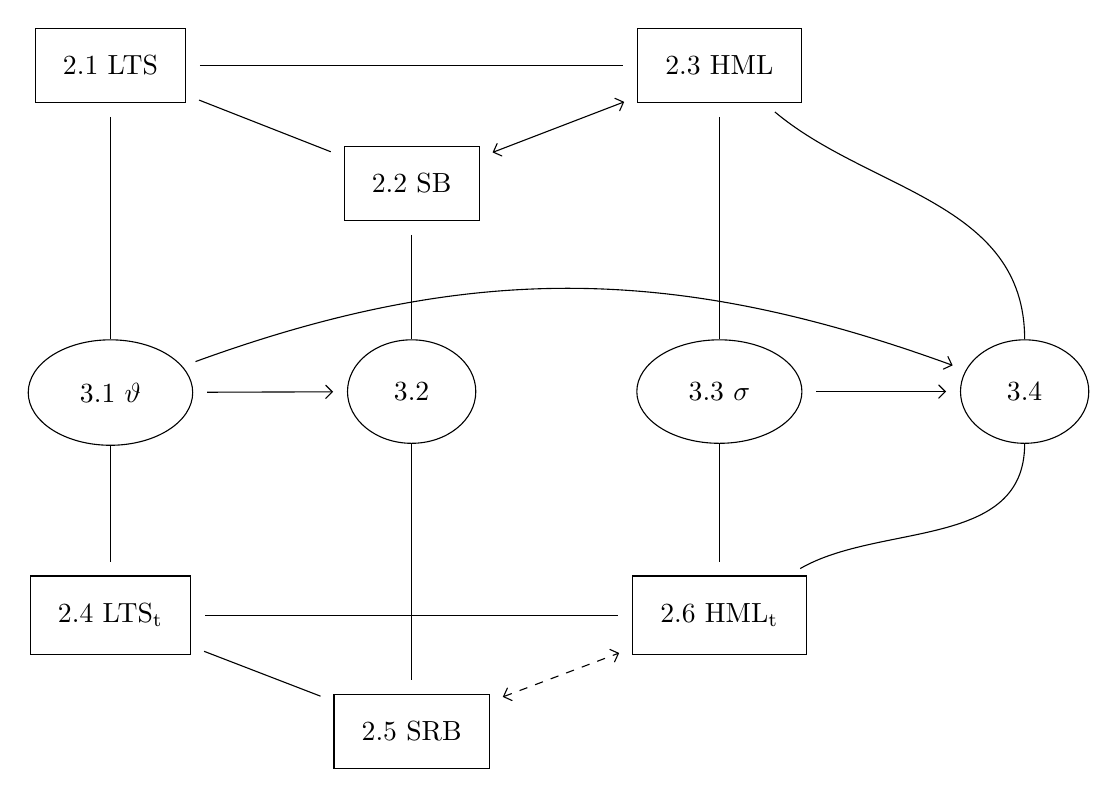
\begin{tikzpicture}[node distance=1cm and 2cm]
    \tikzstyle{every node}=[draw, inner sep=10pt]
    
    \node[rectangle] (21) {2.1 LTS}; 
    \node[rectangle] (22) [right=of 21,yshift=-1.5cm] {2.2 SB}; 
    \node[rectangle] (23) [right=of 22,yshift=1.5cm] {2.3 HML}; 
    
    \node[rectangle] (24) [below=of 21,yshift=-5cm] {2.4 \LTSt{}}; 
    \node[rectangle] (25) [below=of 22,yshift=-5cm] {2.5 SRB}; 
    \node[rectangle] (26) [below=of 23,yshift=-5cm] {2.6 \HMLt{}};
    
    \node[ellipse] (31) [below=of 21,yshift=-2cm] {3.1 $\vartheta$};
    \node[ellipse] (32) [below=of 22,yshift=-0.5cm] {3.2};
    \node[ellipse] (33) [below=of 23,yshift=-2cm] {3.3 $\sigma$};
    \node[ellipse] (34) [right=of 33] {3.4};
    
    \draw [shorten <=5pt,shorten >=5pt] (21) to (22);
    \draw [shorten <=5pt,shorten >=5pt] (21) to (23);
    \draw [<->,>=angle 90,shorten <=5pt,shorten >=5pt] (22) to (23);
    
    \draw [shorten <=5pt,shorten >=5pt] (24) to (25);
    \draw [shorten <=5pt,shorten >=5pt] (24) to (26);
    \draw [<->,dashed,>=angle 90,shorten <=5pt,shorten >=5pt] (25) to (26);
    
    \draw [shorten <=5pt] (21) to (31);
    \draw [shorten <=5pt] (24) to (31);
    \draw [shorten <=5pt] (22) to (32);
    \draw [shorten <=5pt] (25) to (32);
    \draw [shorten <=5pt] (23) to (33);
    \draw [shorten <=5pt] (26) to (33);
    \draw [shorten <=5pt] (23) to[in=90,out=-40] (34);
    \draw [shorten <=5pt] (26) to[in=-90,out=30] (34);
    
    \draw [->,>=angle 90,shorten <=5pt,shorten >=5pt] (31) to (32);
    \draw [->,>=angle 90,shorten <=5pt,shorten >=5pt] (33) to (34);
    \draw [->,>=angle 90,shorten <=5pt,shorten >=5pt] (31) to[out=20,in=160] (34);
\end{tikzpicture}}
\end{center}%
\end{isamarkuptext}\isamarkuptrue%
%
\isadelimtheory
%
\endisadelimtheory
%
\isatagtheory
%
\endisatagtheory
{\isafoldtheory}%
%
\isadelimtheory
%
\endisadelimtheory
%
\end{isabellebody}%
\endinput
%:%file=~/projects/Reducing-Reactive-to-Strong-Bisimilarity/isabelle/Introduction.thy%:%
%:%24=8%:%
%:%36=9%:%
%:%40=11%:%
%:%41=12%:%
%:%42=13%:%
%:%43=14%:%
%:%44=15%:%
%:%45=16%:%
%:%46=17%:%
%:%47=18%:%
%:%48=19%:%
%:%49=20%:%
%:%50=21%:%
%:%51=22%:%
%:%52=23%:%
%:%53=24%:%
%:%54=25%:%
%:%55=26%:%
%:%56=27%:%
%:%57=28%:%
%:%58=29%:%
%:%59=30%:%
%:%60=31%:%
%:%61=32%:%
%:%62=33%:%
%:%63=34%:%
%:%64=35%:%
%:%65=36%:%
%:%66=37%:%
%:%67=38%:%
%:%68=39%:%
%:%69=40%:%
%:%78=42%:%
%:%90=44%:%
%:%91=45%:%
%:%92=46%:%
%:%93=47%:%
%:%94=48%:%
%:%95=49%:%
%:%96=50%:%
%:%97=51%:%
%:%98=52%:%
%:%99=53%:%
%:%108=56%:%
%:%120=59%:%
%:%121=60%:%
%:%122=61%:%
%:%123=62%:%
%:%124=63%:%
%:%125=64%:%
%:%126=65%:%
%:%127=66%:%
%:%128=67%:%
%:%129=68%:%
%:%130=69%:%
%:%131=70%:%
%:%132=71%:%
%:%133=72%:%
%:%134=73%:%
%:%135=74%:%
%:%136=75%:%
%:%137=76%:%
%:%138=77%:%
%:%139=78%:%
%:%140=79%:%
%:%141=80%:%
%:%142=81%:%
%:%143=82%:%
%:%144=83%:%
%:%145=84%:%
%:%146=85%:%
%:%147=86%:%
%:%148=87%:%
%:%149=88%:%
%:%150=89%:%
%:%151=90%:%
%:%152=91%:%
%:%153=92%:%
%:%154=93%:%
%:%155=94%:%
%:%156=95%:%
%:%157=96%:%
%:%158=97%:%
%:%159=98%:%
%
\begin{isabellebody}%
\setisabellecontext{Foundations}%
%
\isadelimtheory
%
\endisadelimtheory
%
\isatagtheory
%
\endisatagtheory
{\isafoldtheory}%
%
\isadelimtheory
%
\endisadelimtheory
%
\isadelimdocument
%
\endisadelimdocument
%
\isatagdocument
%
\isamarkupchapter{Foundations%
}
\isamarkuptrue%
%
\endisatagdocument
{\isafolddocument}%
%
\isadelimdocument
%
\endisadelimdocument
%
\begin{isamarkuptext}%
\label{chap:foundations}%
\end{isamarkuptext}\isamarkuptrue%
%
\begin{isamarkuptext}%
In this section, the concepts that are relevant for the main part of this thesis will be introduced in text, as well as formalised in Isabelle. The formalisations of \cref{sec:LTS,sec:strong_bisimilarity} are based on those done by Benjamin Bisping in \cite{bisping2018computing}; the code is available on GitHub.%
\footnote{see \code{\href{https://coupledsim.bbisping.de/code/}%
{coupledsim.bbisping.de/code/}}}
All other formalisations were done as part of this thesis.%
\end{isamarkuptext}\isamarkuptrue%
%
\isadelimtheory
%
\endisadelimtheory
%
\isatagtheory
%
\endisatagtheory
{\isafoldtheory}%
%
\isadelimtheory
%
\endisadelimtheory
%
\end{isabellebody}%
\endinput
%:%file=~/reactive-bisimilarity-reduction/Foundations.thy%:%
%:%24=7%:%
%:%36=8%:%
%:%40=10%:%
%:%41=11%:%
%:%42=12%:%
%:%43=13%:%
%
\begin{isabellebody}%
\setisabellecontext{Labelled{\isacharunderscore}{\kern0pt}Transition{\isacharunderscore}{\kern0pt}Systems}%
%
\isadelimtheory
%
\endisadelimtheory
%
\isatagtheory
%
\endisatagtheory
{\isafoldtheory}%
%
\isadelimtheory
%
\endisadelimtheory
%
\isadelimdocument
%
\endisadelimdocument
%
\isatagdocument
%
\isamarkupsection{Labelled Transition Systems%
}
\isamarkuptrue%
%
\endisatagdocument
{\isafolddocument}%
%
\isadelimdocument
%
\endisadelimdocument
%
\begin{isamarkuptext}%
\label{sec:LTS}%
\end{isamarkuptext}\isamarkuptrue%
%
\begin{isamarkuptext}%
A Labelled Transition System (LTS) consists of a set of processes (or states) $\Proc$, a set of actions $\Act$, and a relation of transitions $\cdot\xrightarrow{\cdot}\cdot \subseteq \Proc\times\Act\times\Proc$ which directedly connect two processes by an action (the action being the label of the transition) \cite{resyst}. We call a transition labelled by an action $\alpha$ an \emph{$\alpha$-transition}.

LTSs can model reactive systems, as discussed in \cref{chap:introduction}. A process of an LTS, then, corresponds to a momentary state of a reactive system. The outgoing transitions of each process correspond to the actions the reactive system could perform in that state (yielding a subsequent process/state), if facilitated by the environment. The choice between the facilitated transitions of a process is non-deterministic.

This facilitation can be thought of as a set of actions that the environment allows in a given moment, or, more intuitively, as a set of simultaneous inputs from the environment to which the system may react. We call the actions not allowed by the environment in a given moment \emph{blocked}.

The environment can also observe which transitions a system performs and react by changing the set of allowed actions in response.

In classical treatments of LTSs, the actions that the environment allows, blocks, or reacts to, are often considered only implicitly. The reason we put this emphasis on the environment here will become apparent in \cref{sec:LTSt}.

\example{%
The process $p$ can perform any of the $a$-transitions in environments allowing $a$ and the $b$-transition in environments allowing $b$. All derivative (subsequent) states cannot perform any transition.

\lts{
    \node[state]    (p0)                        {$p$};
    \node[state]    (p1) [below left of=p0]     {$p_1$};
    \node[state]    (p2) [below of=p0]          {$p_2$};
    \node[state]    (p3) [below right of=p0]    {$p_3$};
    
    \path   (p0) edge node[above left]          {$a$}   (p1)
                 edge node[above right]         {$a$}   (p2)
                 edge node[above right]         {$b$}   (p3);
}}

A \emph{hidden action}, denoted by $\tau$, allows for additional semantics: a $\tau$-transition can be performed by a process without any interaction from the environment. Depending on the specific semantic context, the performance of a hidden action may also be unobservable (hence the name).%
\end{isamarkuptext}\isamarkuptrue%
%
\isadelimdocument
%
\endisadelimdocument
%
\isatagdocument
%
\isamarkupsubsubsection{Some Definitions%
}
\isamarkuptrue%
%
\endisatagdocument
{\isafolddocument}%
%
\isadelimdocument
%
\endisadelimdocument
%
\begin{isamarkuptext}%
The $\alpha$-derivatives of a state are those states that can be reached with one $\alpha$-transition:
$$\mathit{Der}(p, \alpha) = \{ p' \mid p \xrightarrow{\alpha} p' \}.$$

An LTS is image-finite iff all derivative sets are finite:
$$\forall p \in \Proc, \alpha \in \Act .\; \mathit{Der}(p, \alpha) \text{ is finite}.$$

Similarly, we can say an LTS is image-countable iff all derivative sets are countable:
$$\forall p \in \Proc, \alpha \in \Act .\; \mathit{Der}(p, \alpha) \text{ is countable}.$$%
\end{isamarkuptext}\isamarkuptrue%
%
\isadelimdocument
%
\endisadelimdocument
%
\isatagdocument
%
\isamarkupsubsubsection{Note on Metavariable usage%
}
\isamarkuptrue%
%
\endisatagdocument
{\isafolddocument}%
%
\isadelimdocument
%
\endisadelimdocument
%
\begin{isamarkuptext}%
States of an LTS range over $p, q, p', q', \dots$, where $p$ and $p'$ are used for states connected by some transition (i.e.\@ $p \xrightarrow{\alpha} p'$), whereas $p$ and $q$ are used for states possibly related by some equivalence (e.g.\@ $p \leftrightarrow q$), as will be discussed in the next section.

An arbitrary action of an LTS will be referenced by $\alpha$, whereas an arbitrary \emph{visible} (i.e.\@ non-hidden) action will be referenced by $a$.%
\end{isamarkuptext}\isamarkuptrue%
%
\isadelimdocument
%
\endisadelimdocument
%
\isatagdocument
%
\isamarkupsubsubsection{Practical Example%
}
\isamarkuptrue%
%
\endisatagdocument
{\isafolddocument}%
%
\isadelimdocument
%
\endisadelimdocument
%
\begin{isamarkuptext}%
Let us take a detour away from purely theoretical deliberations and consider a real-world machine that may be modelled as an LTS. We can imagine a very simple snack-selling vending machine that accepts only one type of coin and has individual buttons for each of the snacks. When a coin is inserted and a button pressed, the machine dispenses the desired snack and is then ready to accept coins once again. Because the dispensing of the snack itself requires no interaction from the user, we model it as a $\tau$-transition.

\lts{
    \node[state]    (p0) {$p$};
    \node[state]    (p1) [below of=p0] {$p_1$};
    \node[state]    (p2) [below left of=p1,xshift=-10pt] {$p_2$};
    \node[state]    (p3) [below of=p1] {$p_3$};
    \node[state]    (p4) [below right of=p1,xshift=10pt] {$p_4$};
    
    \path   (p0) edge node[right] {coin} (p1)
            (p1) edge node[above left] {choc} (p2)
                 edge node[right] {nuts} (p3)
                 edge node[above right] {crisps} (p4);
                 
    \draw (p2) to[out=150, in=210, looseness=1, edge node={node [left] {$\tau$}}] (p0);
    \draw (p4) to[out=30, in=-30, looseness=1, edge node={node [right] {$\tau$}}] (p0);
    \draw (p3) to[out=-20, in=0, looseness=2.5, edge node={node [right] {$\tau$}}] (p0);
}
\vspace{-1.5cm}%
\end{isamarkuptext}\isamarkuptrue%
%
\isadelimdocument
%
\endisadelimdocument
%
\isatagdocument
%
\isamarkupsubsection{Isabelle%
}
\isamarkuptrue%
%
\endisatagdocument
{\isafolddocument}%
%
\isadelimdocument
%
\endisadelimdocument
%
\begin{isamarkuptext}%
The sets of states and actions are formalised by type variables \isa{{\isacharprime}{\kern0pt}s} and \isa{{\isacharprime}{\kern0pt}a}, respectively. A specific LTS on these sets is then determined entirely by its set of transitions, denoted by the predicate \isa{tran}. We associate it with a more readable notation (\isa{p\ {\isasymlongmapsto}{\isasymalpha}\ p{\isacharprime}{\kern0pt}} for $p \xrightarrow{\alpha} p'$).%
\end{isamarkuptext}\isamarkuptrue%
\isacommand{locale}\isamarkupfalse%
\ lts\ {\isacharequal}{\kern0pt}\ \isanewline
\ \ \isakeyword{fixes}\ tran\ {\isacharcolon}{\kern0pt}{\isacharcolon}{\kern0pt}\ {\isacartoucheopen}{\isacharprime}{\kern0pt}s\ {\isasymRightarrow}\ {\isacharprime}{\kern0pt}a\ {\isasymRightarrow}\ {\isacharprime}{\kern0pt}s\ {\isasymRightarrow}\ bool{\isacartoucheclose}\ \isanewline
\ \ \ \ {\isacharparenleft}{\kern0pt}{\isachardoublequoteopen}{\isacharunderscore}{\kern0pt}\ {\isasymlongmapsto}{\isacharunderscore}{\kern0pt}\ {\isacharunderscore}{\kern0pt}{\isachardoublequoteclose}\ {\isacharbrackleft}{\kern0pt}{\isadigit{7}}{\isadigit{0}}{\isacharcomma}{\kern0pt}\ {\isadigit{7}}{\isadigit{0}}{\isacharcomma}{\kern0pt}\ {\isadigit{7}}{\isadigit{0}}{\isacharbrackright}{\kern0pt}\ {\isadigit{8}}{\isadigit{0}}{\isacharparenright}{\kern0pt}\isanewline
\isakeyword{begin}%
\begin{isamarkuptext}%
The other definitions can be formalised in a straightforward manner.%
\end{isamarkuptext}\isamarkuptrue%
\isacommand{abbreviation}\isamarkupfalse%
\ derivatives\ {\isacharcolon}{\kern0pt}{\isacharcolon}{\kern0pt}\ {\isacartoucheopen}{\isacharprime}{\kern0pt}s\ {\isasymRightarrow}\ {\isacharprime}{\kern0pt}a\ {\isasymRightarrow}\ {\isacharprime}{\kern0pt}s\ set{\isacartoucheclose}\ \isanewline
\ \ {\isacharparenleft}{\kern0pt}{\isacartoucheopen}Der{\isacharprime}{\kern0pt}{\isacharparenleft}{\kern0pt}{\isacharunderscore}{\kern0pt}{\isacharcomma}{\kern0pt}\ {\isacharunderscore}{\kern0pt}{\isacharprime}{\kern0pt}{\isacharparenright}{\kern0pt}{\isacartoucheclose}\ {\isacharbrackleft}{\kern0pt}{\isadigit{5}}{\isadigit{0}}{\isacharcomma}{\kern0pt}\ {\isadigit{5}}{\isadigit{0}}{\isacharbrackright}{\kern0pt}\ {\isadigit{1}}{\isadigit{0}}{\isadigit{0}}{\isadigit{0}}{\isacharparenright}{\kern0pt}\isanewline
\ \ \isakeyword{where}\ {\isacartoucheopen}Der{\isacharparenleft}{\kern0pt}p{\isacharcomma}{\kern0pt}\ {\isasymalpha}{\isacharparenright}{\kern0pt}\ {\isasymequiv}\ {\isacharbraceleft}{\kern0pt}p{\isacharprime}{\kern0pt}{\isachardot}{\kern0pt}\ p\ {\isasymlongmapsto}{\isasymalpha}\ p{\isacharprime}{\kern0pt}{\isacharbraceright}{\kern0pt}{\isacartoucheclose}\isanewline
\isanewline
\isacommand{definition}\isamarkupfalse%
\ image{\isacharunderscore}{\kern0pt}finite\ {\isacharcolon}{\kern0pt}{\isacharcolon}{\kern0pt}\ {\isacartoucheopen}bool{\isacartoucheclose}\isanewline
\ \ \isakeyword{where}\ {\isacartoucheopen}image{\isacharunderscore}{\kern0pt}finite\ {\isasymequiv}\ {\isacharparenleft}{\kern0pt}{\isasymforall}\ p\ {\isasymalpha}{\isachardot}{\kern0pt}\ finite\ Der{\isacharparenleft}{\kern0pt}p{\isacharcomma}{\kern0pt}\ {\isasymalpha}{\isacharparenright}{\kern0pt}{\isacharparenright}{\kern0pt}{\isacartoucheclose}\isanewline
\isacommand{definition}\isamarkupfalse%
\ image{\isacharunderscore}{\kern0pt}countable\ {\isacharcolon}{\kern0pt}{\isacharcolon}{\kern0pt}\ {\isacartoucheopen}bool{\isacartoucheclose}\isanewline
\ \ \isakeyword{where}\ {\isacartoucheopen}image{\isacharunderscore}{\kern0pt}countable\ {\isasymequiv}\ {\isacharparenleft}{\kern0pt}{\isasymforall}\ p\ {\isasymalpha}{\isachardot}{\kern0pt}\ countable\ Der{\isacharparenleft}{\kern0pt}p{\isacharcomma}{\kern0pt}\ {\isasymalpha}{\isacharparenright}{\kern0pt}{\isacharparenright}{\kern0pt}{\isacartoucheclose}%
\begin{isamarkuptext}%
These two properties concern the entire LTS at hand (given by the locale context) and will be useful when we want to state propositions that only hold for LTSs that satisfy these properties.%
\end{isamarkuptext}\isamarkuptrue%
\isacommand{end}\isamarkupfalse%
\ %
\isamarkupcmt{of \isa{locale\ lts}%
}%
\begin{isamarkuptext}%
We formalise LTSs with hidden actions as an extension of ordinary LTSs with a fixed action \isa{{\isasymtau}}.%
\end{isamarkuptext}\isamarkuptrue%
\isacommand{locale}\isamarkupfalse%
\ lts{\isacharunderscore}{\kern0pt}tau\ {\isacharequal}{\kern0pt}\ lts\ tran\ \isanewline
\ \ \isakeyword{for}\ tran\ {\isacharcolon}{\kern0pt}{\isacharcolon}{\kern0pt}\ {\isacartoucheopen}{\isacharprime}{\kern0pt}s\ {\isasymRightarrow}\ {\isacharprime}{\kern0pt}a\ {\isasymRightarrow}\ {\isacharprime}{\kern0pt}s\ {\isasymRightarrow}\ bool{\isacartoucheclose}\ {\isacharplus}{\kern0pt}\ \isanewline
\ \ \isakeyword{fixes}\ {\isasymtau}\ {\isacharcolon}{\kern0pt}{\isacharcolon}{\kern0pt}\ {\isacartoucheopen}{\isacharprime}{\kern0pt}a{\isacartoucheclose}\isanewline
%
\isadelimtheory
%
\endisadelimtheory
%
\isatagtheory
%
\endisatagtheory
{\isafoldtheory}%
%
\isadelimtheory
%
\endisadelimtheory
%
\end{isabellebody}%
\endinput
%:%file=~/projects/Reducing-Reactive-to-Strong-Bisimilarity/isabelle/Labelled_Transition_Systems.thy%:%
%:%24=14%:%
%:%36=15%:%
%:%40=17%:%
%:%41=18%:%
%:%42=19%:%
%:%43=20%:%
%:%44=21%:%
%:%45=22%:%
%:%46=23%:%
%:%47=24%:%
%:%48=25%:%
%:%49=26%:%
%:%50=27%:%
%:%51=28%:%
%:%52=29%:%
%:%53=30%:%
%:%54=31%:%
%:%55=32%:%
%:%56=33%:%
%:%57=34%:%
%:%58=35%:%
%:%59=36%:%
%:%60=37%:%
%:%61=38%:%
%:%62=39%:%
%:%63=40%:%
%:%64=41%:%
%:%73=43%:%
%:%85=45%:%
%:%86=46%:%
%:%87=47%:%
%:%88=48%:%
%:%89=49%:%
%:%90=50%:%
%:%91=51%:%
%:%92=52%:%
%:%101=54%:%
%:%113=56%:%
%:%114=57%:%
%:%115=58%:%
%:%124=60%:%
%:%136=62%:%
%:%137=63%:%
%:%138=64%:%
%:%139=65%:%
%:%140=66%:%
%:%141=67%:%
%:%142=68%:%
%:%143=69%:%
%:%144=70%:%
%:%145=71%:%
%:%146=72%:%
%:%147=73%:%
%:%148=74%:%
%:%149=75%:%
%:%150=76%:%
%:%151=77%:%
%:%152=78%:%
%:%153=79%:%
%:%154=80%:%
%:%163=83%:%
%:%175=85%:%
%:%177=87%:%
%:%178=87%:%
%:%179=88%:%
%:%180=89%:%
%:%181=90%:%
%:%183=92%:%
%:%185=94%:%
%:%186=94%:%
%:%187=95%:%
%:%188=96%:%
%:%189=97%:%
%:%190=98%:%
%:%191=98%:%
%:%192=99%:%
%:%193=100%:%
%:%194=100%:%
%:%195=101%:%
%:%197=103%:%
%:%199=105%:%
%:%200=105%:%
%:%201=105%:%
%:%204=108%:%
%:%206=110%:%
%:%207=110%:%
%:%208=111%:%
%:%209=112%:%
%
\begin{isabellebody}%
\setisabellecontext{Strong{\isacharunderscore}{\kern0pt}Bisimilarity}%
%
\isadelimtheory
%
\endisadelimtheory
%
\isatagtheory
%
\endisatagtheory
{\isafoldtheory}%
%
\isadelimtheory
%
\endisadelimtheory
%
\isadelimdocument
%
\endisadelimdocument
%
\isatagdocument
%
\isamarkupsection{Strong Bisimilarity%
}
\isamarkuptrue%
%
\endisatagdocument
{\isafolddocument}%
%
\isadelimdocument
%
\endisadelimdocument
%
\begin{isamarkuptext}%
\label{sec:strong_bisimilarity}%
\end{isamarkuptext}\isamarkuptrue%
%
\begin{isamarkuptext}%
As discussed in the previous section, LTSs can describe the behaviour of reactive systems, and this behaviour is observable by the environment (in terms of the transitions performed by the system). This begets a notion of behavioural equivalence, where two processes are said to be behaviourally equivalent if they exhibit the same (observable) behaviour \cite{reactivesystems}.

Bisimilarity (or \emph{strong bisimilarity}, to be precise) is the \enquote{\emph{finest extensional behavioural equivalence} \textelp{} on processes} \cite[section 0.1]{introBC}, an extensional property being one that treats the system in question as a black box, i.e.\@ the specific state space of the system remains hidden and performed transitions are only observable in terms of their action-label. This distinguishes bisimilarity from stronger graph equivalences like \emph{graph isomorphism}, where the (intensional) identity of processes (graph nodes) is relevant \cite{advBC_origins}.

\example{%
The processes $p$ and $q$ are strongly bisimilar (written $p \leftrightarrow q$, following \cite{rbs}), as both can always perform exactly two a-transitions and no further transitions afterwards. There is no isomorphism between the left and right subgraphs, as they have a different number of nodes.

\lts{
    \node[state]    (p0)                            {$p$};
    \node[state]    (p1) [below left of=p0]         {$p_1$};
    \node[state]    (p2) [below of=p1]              {$p_2$};
    \node[state]    (p3) [below right of=p0]        {$p_3$};
    \node[state]    (p4) [below of=p3]              {$p_4$};
    \node[state]    (q0) [right of=p0,xshift=2cm]   {$q$};
    \node[state]    (q1) [below of=q0]              {$q_1$};
    \node[state]    (q2) [below of=q1]              {$q_2$};
    
    \path   (p0) edge node[above left]  {$a$}   (p1)
                 edge node              {$a$}   (p3)
            (p1) edge node[left]        {$a$}   (p2)
            (p3) edge node[left]        {$a$}   (p4)
            (q0) edge node              {$a$}   (q1)
            (q1) edge node              {$a$}   (q2);
}}

\pagebreak
It is important to note that not only transitions that are performable, but also those that are not, are relevant.

\example{%
The processes $p$ and $q$ are not strongly bisimilar, as $p$ can perform an $a$-transition into a subsequent state, where it can perform no further transitions, whereas $q$ can always perform two $a$-transitions in sequence.

\lts{
    \node[state]    (p0)                            {$p$};
    \node[state]    (p1) [below left of=p0]         {$p_1$};
    \node[state]    (p2) [below of=p1]              {$p_2$};
    \node[state]    (p3) [below right of=p0]        {$p_3$};
    \node[state]    (q0) [right of=p0,xshift=2cm]   {$q$};
    \node[state]    (q1) [below of=q0]              {$q_1$};
    \node[state]    (q2) [below of=q1]              {$q_2$};
    
    \path   (p0) edge node[above left]  {$a$}   (p1)
                 edge node              {$a$}   (p3)
            (p1) edge node[left]        {$a$}   (p2)
            (q0) edge node              {$a$}   (q1)
            (q1) edge node              {$a$}   (q2);
}}

Strong bisimilarity is the \emph{finest} extensional behavioural equivalence, because all actions are thought of as observable. An example of a coarser equivalence is \emph{weak bisimilarity}, which treats the aforementioned hidden action $\tau$ as unobservable. However, weak bisimilarity is of no further relevance for this thesis and the interested reader is referred to \cite[Chapter 3.4]{reactivesystems}.

The notion of strong bisimilarity can be formalised through \emph{strong bisimulation} (SB) relations, introduced originally by David Park in \cite{park81}. A binary relation $\mathcal{R}$ over the set of processes $\Proc$ is an SB iff for all $(p,q) \in \mathcal{R}$:
\begin{align*}
&\forall p' \in \Proc,\; \alpha \in \Act .\; p \xrightarrow{\alpha} p' \longrightarrow
\exists q' \in \Proc .\; q \xrightarrow{\alpha} q' \wedge (p',q') \in \mathcal{R}, \text{ and}\\
&\forall q' \in \Proc,\; \alpha \in \Act .\; q \xrightarrow{\alpha} q' \longrightarrow
\exists p' \in \Proc .\; p \xrightarrow{\alpha} p' \wedge (p',q') \in \mathcal{R}.
\end{align*}%
\end{isamarkuptext}\isamarkuptrue%
%
\isadelimdocument
%
\endisadelimdocument
%
\isatagdocument
%
\isamarkupsubsection{Isabelle%
}
\isamarkuptrue%
%
\endisatagdocument
{\isafolddocument}%
%
\isadelimdocument
%
\endisadelimdocument
%
\begin{isamarkuptext}%
Strong bisimulations are straightforward to formalise in Isabelle, using the \enquote{curried} definition approach discussed in \cref{chap:isabelle}.%
\end{isamarkuptext}\isamarkuptrue%
\isacommand{context}\isamarkupfalse%
\ lts\ \isakeyword{begin}\isanewline
\isanewline
%
\isamarkupcmt{strong bisimulation%
}\isanewline
\isacommand{definition}\isamarkupfalse%
\ SB\ {\isacharcolon}{\kern0pt}{\isacharcolon}{\kern0pt}\ {\isacartoucheopen}{\isacharparenleft}{\kern0pt}{\isacharprime}{\kern0pt}s\ {\isasymRightarrow}\ {\isacharprime}{\kern0pt}s\ {\isasymRightarrow}\ bool{\isacharparenright}{\kern0pt}\ {\isasymRightarrow}\ bool{\isacartoucheclose}\isanewline
\ \ \isakeyword{where}\ {\isacartoucheopen}SB\ R\ {\isasymequiv}\ {\isasymforall}\ p\ q{\isachardot}{\kern0pt}\ R\ p\ q\ {\isasymlongrightarrow}\ \isanewline
\ \ \ \ {\isacharparenleft}{\kern0pt}{\isasymforall}\ p{\isacharprime}{\kern0pt}\ {\isasymalpha}{\isachardot}{\kern0pt}\ p\ {\isasymlongmapsto}{\isasymalpha}\ p{\isacharprime}{\kern0pt}\ {\isasymlongrightarrow}\ {\isacharparenleft}{\kern0pt}{\isasymexists}\ q{\isacharprime}{\kern0pt}{\isachardot}{\kern0pt}\ {\isacharparenleft}{\kern0pt}q\ {\isasymlongmapsto}{\isasymalpha}\ q{\isacharprime}{\kern0pt}{\isacharparenright}{\kern0pt}\ {\isasymand}\ R\ p{\isacharprime}{\kern0pt}\ q{\isacharprime}{\kern0pt}{\isacharparenright}{\kern0pt}{\isacharparenright}{\kern0pt}\ {\isasymand}\isanewline
\ \ \ \ {\isacharparenleft}{\kern0pt}{\isasymforall}\ q{\isacharprime}{\kern0pt}\ {\isasymalpha}{\isachardot}{\kern0pt}\ q\ {\isasymlongmapsto}{\isasymalpha}\ q{\isacharprime}{\kern0pt}\ {\isasymlongrightarrow}\ {\isacharparenleft}{\kern0pt}{\isasymexists}\ p{\isacharprime}{\kern0pt}{\isachardot}{\kern0pt}\ {\isacharparenleft}{\kern0pt}p\ {\isasymlongmapsto}{\isasymalpha}\ p{\isacharprime}{\kern0pt}{\isacharparenright}{\kern0pt}\ {\isasymand}\ R\ p{\isacharprime}{\kern0pt}\ q{\isacharprime}{\kern0pt}{\isacharparenright}{\kern0pt}{\isacharparenright}{\kern0pt}{\isacartoucheclose}%
\begin{isamarkuptext}%
\pagebreak
Two processes $p$ and $q$ are then strongly bisimilar iff there is an SB that contains the pair $(p, q)$.%
\end{isamarkuptext}\isamarkuptrue%
\isacommand{definition}\isamarkupfalse%
\ strongly{\isacharunderscore}{\kern0pt}bisimilar\ {\isacharcolon}{\kern0pt}{\isacharcolon}{\kern0pt}\ {\isacartoucheopen}{\isacharprime}{\kern0pt}s\ {\isasymRightarrow}\ {\isacharprime}{\kern0pt}s\ {\isasymRightarrow}\ bool{\isacartoucheclose}\ \isanewline
\ \ {\isacharparenleft}{\kern0pt}{\isacartoucheopen}{\isacharunderscore}{\kern0pt}\ {\isasymleftrightarrow}\ {\isacharunderscore}{\kern0pt}{\isacartoucheclose}\ {\isacharbrackleft}{\kern0pt}{\isadigit{7}}{\isadigit{0}}{\isacharcomma}{\kern0pt}\ {\isadigit{7}}{\isadigit{0}}{\isacharbrackright}{\kern0pt}\ {\isadigit{7}}{\isadigit{0}}{\isacharparenright}{\kern0pt}\isanewline
\ \ \isakeyword{where}\ {\isacartoucheopen}p\ {\isasymleftrightarrow}\ q\ {\isasymequiv}\ {\isasymexists}\ R{\isachardot}{\kern0pt}\ SB\ R\ {\isasymand}\ R\ p\ q{\isacartoucheclose}%
\begin{isamarkuptext}%
The following corollaries are immediate consequences of these definitions.%
\end{isamarkuptext}\isamarkuptrue%
\isacommand{corollary}\isamarkupfalse%
\ strongly{\isacharunderscore}{\kern0pt}bisimilar{\isacharunderscore}{\kern0pt}step{\isacharcolon}{\kern0pt}\isanewline
\ \ \isakeyword{assumes}\ \isanewline
\ \ \ \ {\isacartoucheopen}p\ {\isasymleftrightarrow}\ q{\isacartoucheclose}\isanewline
\ \ \isakeyword{shows}\isanewline
\ \ \ \ {\isacartoucheopen}p\ {\isasymlongmapsto}a\ p{\isacharprime}{\kern0pt}\ {\isasymLongrightarrow}\ {\isacharparenleft}{\kern0pt}{\isasymexists}\ q{\isacharprime}{\kern0pt}{\isachardot}{\kern0pt}\ {\isacharparenleft}{\kern0pt}q\ {\isasymlongmapsto}a\ q{\isacharprime}{\kern0pt}{\isacharparenright}{\kern0pt}\ {\isasymand}\ p{\isacharprime}{\kern0pt}\ {\isasymleftrightarrow}\ q{\isacharprime}{\kern0pt}{\isacharparenright}{\kern0pt}{\isacartoucheclose}\isanewline
\ \ \ \ {\isacartoucheopen}q\ {\isasymlongmapsto}a\ q{\isacharprime}{\kern0pt}\ {\isasymLongrightarrow}\ {\isacharparenleft}{\kern0pt}{\isasymexists}\ p{\isacharprime}{\kern0pt}{\isachardot}{\kern0pt}\ {\isacharparenleft}{\kern0pt}p\ {\isasymlongmapsto}a\ p{\isacharprime}{\kern0pt}{\isacharparenright}{\kern0pt}\ {\isasymand}\ p{\isacharprime}{\kern0pt}\ {\isasymleftrightarrow}\ q{\isacharprime}{\kern0pt}{\isacharparenright}{\kern0pt}{\isacartoucheclose}\isanewline
%
\isadelimproof
\ \ %
\endisadelimproof
%
\isatagproof
\isacommand{using}\isamarkupfalse%
\ assms\ SB{\isacharunderscore}{\kern0pt}def\ strongly{\isacharunderscore}{\kern0pt}bisimilar{\isacharunderscore}{\kern0pt}def\ \isacommand{by}\isamarkupfalse%
\ {\isacharparenleft}{\kern0pt}smt\ {\isacharparenleft}{\kern0pt}verit{\isacharparenright}{\kern0pt}{\isacharparenright}{\kern0pt}{\isacharplus}{\kern0pt}%
\endisatagproof
{\isafoldproof}%
%
\isadelimproof
\isanewline
%
\endisadelimproof
\ \ \isanewline
\isacommand{corollary}\isamarkupfalse%
\ strongly{\isacharunderscore}{\kern0pt}bisimilar{\isacharunderscore}{\kern0pt}symm{\isacharcolon}{\kern0pt}\isanewline
\ \ \isakeyword{assumes}\ {\isacartoucheopen}p\ {\isasymleftrightarrow}\ q{\isacartoucheclose}\ \isanewline
\ \ \isakeyword{shows}\ {\isacartoucheopen}q\ {\isasymleftrightarrow}\ p{\isacartoucheclose}\ \isanewline
%
\isadelimproof
\ \ %
\endisadelimproof
%
\isatagproof
\isacommand{using}\isamarkupfalse%
\ assms\ \isacommand{unfolding}\isamarkupfalse%
\ strongly{\isacharunderscore}{\kern0pt}bisimilar{\isacharunderscore}{\kern0pt}def\isanewline
\isacommand{proof}\isamarkupfalse%
\isanewline
\ \ \isacommand{fix}\isamarkupfalse%
\ R\isanewline
\ \ \isacommand{assume}\isamarkupfalse%
\ {\isacartoucheopen}SB\ R\ {\isasymand}\ R\ p\ q{\isacartoucheclose}\isanewline
\ \ \isacommand{let}\isamarkupfalse%
\ {\isacharquery}{\kern0pt}R{\isacharprime}{\kern0pt}\ {\isacharequal}{\kern0pt}\ {\isacartoucheopen}{\isasymlambda}\ a\ b{\isachardot}{\kern0pt}\ R\ b\ a{\isacartoucheclose}\isanewline
\ \ \isacommand{have}\isamarkupfalse%
\ {\isacartoucheopen}SB\ {\isacharquery}{\kern0pt}R{\isacharprime}{\kern0pt}\ {\isasymand}\ {\isacharquery}{\kern0pt}R{\isacharprime}{\kern0pt}\ q\ p{\isacartoucheclose}\ \isacommand{using}\isamarkupfalse%
\ SB{\isacharunderscore}{\kern0pt}def\ {\isacartoucheopen}SB\ R\ {\isasymand}\ R\ p\ q{\isacartoucheclose}\ \isacommand{by}\isamarkupfalse%
\ presburger\isanewline
\ \ \isacommand{thus}\isamarkupfalse%
\ {\isacartoucheopen}{\isasymexists}R{\isachardot}{\kern0pt}\ SB\ R\ {\isasymand}\ R\ q\ p{\isacartoucheclose}\ \isacommand{by}\isamarkupfalse%
\ auto\isanewline
\isacommand{qed}\isamarkupfalse%
%
\endisatagproof
{\isafoldproof}%
%
\isadelimproof
\isanewline
%
\endisadelimproof
\isanewline
\isacommand{end}\isamarkupfalse%
\ %
\isamarkupcmt{context lts%
}%
\isadelimtheory
%
\endisadelimtheory
%
\isatagtheory
%
\endisatagtheory
{\isafoldtheory}%
%
\isadelimtheory
%
\endisadelimtheory
%
\end{isabellebody}%
\endinput
%:%file=~/projects/Reducing-Reactive-to-Strong-Bisimilarity/isabelle/Strong_Bisimilarity.thy%:%
%:%24=7%:%
%:%36=8%:%
%:%40=10%:%
%:%41=11%:%
%:%42=12%:%
%:%43=13%:%
%:%44=14%:%
%:%45=15%:%
%:%46=16%:%
%:%47=17%:%
%:%48=18%:%
%:%49=19%:%
%:%50=20%:%
%:%51=21%:%
%:%52=22%:%
%:%53=23%:%
%:%54=24%:%
%:%55=25%:%
%:%56=26%:%
%:%57=27%:%
%:%58=28%:%
%:%59=29%:%
%:%60=30%:%
%:%61=31%:%
%:%62=32%:%
%:%63=33%:%
%:%64=34%:%
%:%65=35%:%
%:%66=36%:%
%:%67=37%:%
%:%68=38%:%
%:%69=39%:%
%:%70=40%:%
%:%71=41%:%
%:%72=42%:%
%:%73=43%:%
%:%74=44%:%
%:%75=45%:%
%:%76=46%:%
%:%77=47%:%
%:%78=48%:%
%:%79=49%:%
%:%80=50%:%
%:%81=51%:%
%:%82=52%:%
%:%83=53%:%
%:%84=54%:%
%:%85=55%:%
%:%86=56%:%
%:%87=57%:%
%:%88=58%:%
%:%89=59%:%
%:%90=60%:%
%:%91=61%:%
%:%92=62%:%
%:%93=63%:%
%:%94=64%:%
%:%95=65%:%
%:%104=68%:%
%:%116=70%:%
%:%118=72%:%
%:%119=72%:%
%:%120=73%:%
%:%122=74%:%
%:%123=74%:%
%:%124=75%:%
%:%125=75%:%
%:%126=76%:%
%:%130=80%:%
%:%131=81%:%
%:%133=83%:%
%:%134=83%:%
%:%135=84%:%
%:%136=85%:%
%:%138=87%:%
%:%140=89%:%
%:%141=89%:%
%:%142=90%:%
%:%143=91%:%
%:%144=92%:%
%:%145=93%:%
%:%146=94%:%
%:%149=95%:%
%:%153=95%:%
%:%154=95%:%
%:%155=95%:%
%:%160=95%:%
%:%163=96%:%
%:%164=97%:%
%:%165=97%:%
%:%166=98%:%
%:%167=99%:%
%:%170=100%:%
%:%174=100%:%
%:%175=100%:%
%:%176=100%:%
%:%177=101%:%
%:%178=101%:%
%:%179=102%:%
%:%180=102%:%
%:%181=103%:%
%:%182=103%:%
%:%183=104%:%
%:%184=104%:%
%:%185=105%:%
%:%186=105%:%
%:%187=105%:%
%:%188=105%:%
%:%189=106%:%
%:%190=106%:%
%:%191=106%:%
%:%192=107%:%
%:%198=107%:%
%:%201=108%:%
%:%202=109%:%
%:%203=109%:%
%:%204=109%:%
%
\begin{isabellebody}%
\setisabellecontext{HM{\isacharunderscore}{\kern0pt}Logic}%
%
\isadelimtheory
%
\endisadelimtheory
%
\isatagtheory
%
\endisatagtheory
{\isafoldtheory}%
%
\isadelimtheory
%
\endisadelimtheory
%
\isadelimdocument
%
\endisadelimdocument
%
\isatagdocument
%
\isamarkupsection{Hennessy-Milner Logic%
}
\isamarkuptrue%
%
\endisatagdocument
{\isafolddocument}%
%
\isadelimdocument
%
\endisadelimdocument
%
\begin{isamarkuptext}%
\label{sec:HML}%
\end{isamarkuptext}\isamarkuptrue%
%
\begin{isamarkuptext}%
In their seminal paper \cite{hm85}, Matthew Hennessy and Robin Milner present a modal-logical characterisation of strong bisimilarity (although they do not call it that), by process properties: \enquote{two processes are equivalent if and only if they enjoy the same set of properties.} These properties are expressed as terms of a modal-logical language, consisting merely of (finite) conjunction, negation, and a family of modal possibility operators. This language is known today as Hennessy-Milner logic (HML), with formulas $\varphi$ defined by the following grammar (where $\alpha$ ranges over the set of actions $\Act$):
$$\varphi ::= t\!t \mid \varphi_1 \;\wedge\; \varphi_2 \mid \neg\varphi \mid \langle\alpha\rangle\varphi$$

The semantics (on LTS processes) is given as follows: all processes satisfy $t\!t$, $\varphi_1 \;\wedge\; \varphi_2$ is satisfied if both $\varphi_1$ and $\varphi_2$ are satisfied, $\neg\varphi$ is satisfied if $\varphi$ is not satisfied, and $\langle\alpha\rangle\varphi$ is satisfied by a process if it is possible to do an $\alpha$-transition into a process that satisfies $\varphi$.

\cite{hm85} also contains the proof that this modal-logical characterisation of strong bisimilarity coincides with a characterisation that is effectively the same as the one we saw in \cref{sec:strong_bisimilarity} using strong bisimulations. Although they use different terminology, their result can be summarised as follows: for image-finite LTSs, two processes are strongly bisimilar iff they satisfy the same set of HML formulas. We call this the \emph{modal characterisation} of strong bisimilarity.

Let the \emph{cardinality of conjunction} be the maximally allowed cardinality of sets of formulas conjoined under a conjunction term (for a given variant of HML). For the simple variant above, conjunction has finite cardinality. By allowing for conjunction of arbitrary cardinality (infinitary HML), the modal characterisation of strong bisimilarity can be proved for arbitrary LTSs. This is done in \cref{chap:HML_infinitary}.

In this section, however, conjunction is constrained to be of countable cardinality, as this turned out to be significantly easier to deal with in the upcoming proofs. The modal characterisation of strong bisimilarity, then, works for LTSs that are image-countable, as we shall see below.

Formulas $\varphi$ are given by the following grammar, where $I$ ranges over all subsets of the natural numbers $\mathbb{N}$:
$$\varphi ::= \textstyle\bigwedge_{i \in I} \varphi_i \mid \neg\varphi \mid \langle\alpha\rangle\varphi$$

The semantics of HML formulas on LTSs are as above, with the alteration that a process satisfies $\bigwedge_{i \in I} \varphi_i$ iff it satisfies $\varphi_i$ for all $i \in I$.

Additional operators can be added as \enquote{syntactic sugar} as follows:
\begin{align*}
    t\!t &\equiv \textstyle\bigwedge_{i \in \emptyset} \varphi_i \\
    f\!\!f &\equiv \neg t\!t \\
    \textstyle\bigvee_{i \in I} \varphi_i &\equiv \neg \textstyle\bigwedge_{i \in I} \neg\varphi_i
\end{align*}%
\end{isamarkuptext}\isamarkuptrue%
%
\isadelimdocument
%
\endisadelimdocument
%
\isatagdocument
%
\isamarkupsubsection{Isabelle%
}
\isamarkuptrue%
%
\isamarkupsubsubsection{Syntax%
}
\isamarkuptrue%
%
\endisatagdocument
{\isafolddocument}%
%
\isadelimdocument
%
\endisadelimdocument
%
\begin{isamarkuptext}%
By definition of countability, all countable sets of formulas can be given by $\{\varphi_i\}_{i \in I} =: \Phi$ for some $I \subseteq \mathbb{N}$ (then $\bigwedge_{i \in I} \varphi_i$ corresponds to $\bigwedge \Phi$). Therefore, the following data type (parameterised by the type of actions \isa{{\isacharprime}{\kern0pt}a}) formalises the definition of HML formulas above (\isa{cset} is the type constructor for countable sets; \isa{acset} and \isa{rcset} are the type morphisms between the types \isa{set} and \isa{cset}; more details below).

I abstained from assigning the constructors a more readable symbolic notation because of the ambiguities and name clashes that would ensue in upcoming sections. The symbolic notations after the constructors below are just code comments.%
\end{isamarkuptext}\isamarkuptrue%
\isacommand{datatype}\isamarkupfalse%
\ {\isacharparenleft}{\kern0pt}{\isacharprime}{\kern0pt}a{\isacharparenright}{\kern0pt}HML{\isacharunderscore}{\kern0pt}formula\ {\isacharequal}{\kern0pt}\isanewline
\ \ HML{\isacharunderscore}{\kern0pt}conj\ \ {\isacartoucheopen}{\isacharparenleft}{\kern0pt}{\isacharprime}{\kern0pt}a{\isacharparenright}{\kern0pt}HML{\isacharunderscore}{\kern0pt}formula\ cset{\isacartoucheclose}\ %
\isamarkupcmt{$\bigwedge \Phi$%
}\ \isanewline
{\isacharbar}{\kern0pt}\ HML{\isacharunderscore}{\kern0pt}neg\ \ \ {\isacartoucheopen}{\isacharparenleft}{\kern0pt}{\isacharprime}{\kern0pt}a{\isacharparenright}{\kern0pt}HML{\isacharunderscore}{\kern0pt}formula{\isacartoucheclose}\ %
\isamarkupcmt{$\neg\varphi$%
}\ \isanewline
{\isacharbar}{\kern0pt}\ HML{\isacharunderscore}{\kern0pt}poss\ \ {\isacartoucheopen}{\isacharprime}{\kern0pt}a{\isacartoucheclose}\ {\isacartoucheopen}{\isacharparenleft}{\kern0pt}{\isacharprime}{\kern0pt}a{\isacharparenright}{\kern0pt}HML{\isacharunderscore}{\kern0pt}formula{\isacartoucheclose}\ %
\isamarkupcmt{$\langle\alpha\rangle\varphi$%
}%
\begin{isamarkuptext}%
The following abbreviations introduce useful constants as syntactic sugar.%
\end{isamarkuptext}\isamarkuptrue%
\isacommand{abbreviation}\isamarkupfalse%
\ HML{\isacharunderscore}{\kern0pt}true\ {\isacharcolon}{\kern0pt}{\isacharcolon}{\kern0pt}\ {\isacartoucheopen}{\isacharparenleft}{\kern0pt}{\isacharprime}{\kern0pt}a{\isacharparenright}{\kern0pt}HML{\isacharunderscore}{\kern0pt}formula{\isacartoucheclose}\ %
\isamarkupcmt{$t\!t$%
}\isanewline
\ \ \isakeyword{where}\ {\isacartoucheopen}HML{\isacharunderscore}{\kern0pt}true\ {\isasymequiv}\ HML{\isacharunderscore}{\kern0pt}conj\ {\isacharparenleft}{\kern0pt}acset\ {\isasymemptyset}{\isacharparenright}{\kern0pt}{\isacartoucheclose}\isanewline
\isacommand{abbreviation}\isamarkupfalse%
\ HML{\isacharunderscore}{\kern0pt}false\ {\isacharcolon}{\kern0pt}{\isacharcolon}{\kern0pt}\ {\isacartoucheopen}{\isacharparenleft}{\kern0pt}{\isacharprime}{\kern0pt}a{\isacharparenright}{\kern0pt}HML{\isacharunderscore}{\kern0pt}formula{\isacartoucheclose}\ %
\isamarkupcmt{$f\!\!f$%
}\isanewline
\ \ \isakeyword{where}\ {\isacartoucheopen}HML{\isacharunderscore}{\kern0pt}false\ {\isasymequiv}\ HML{\isacharunderscore}{\kern0pt}neg\ HML{\isacharunderscore}{\kern0pt}true{\isacartoucheclose}\isanewline
\isacommand{abbreviation}\isamarkupfalse%
\ HML{\isacharunderscore}{\kern0pt}disj\ {\isacharcolon}{\kern0pt}{\isacharcolon}{\kern0pt}\ {\isacartoucheopen}{\isacharparenleft}{\kern0pt}{\isacharprime}{\kern0pt}a{\isacharparenright}{\kern0pt}HML{\isacharunderscore}{\kern0pt}formula\ cset\ {\isasymRightarrow}\ {\isacharparenleft}{\kern0pt}{\isacharprime}{\kern0pt}a{\isacharparenright}{\kern0pt}HML{\isacharunderscore}{\kern0pt}formula{\isacartoucheclose}\ %
\isamarkupcmt{$\bigvee \Phi$%
}\isanewline
\ \ \isakeyword{where}\ {\isacartoucheopen}HML{\isacharunderscore}{\kern0pt}disj\ {\isasymPhi}\ {\isasymequiv}\ HML{\isacharunderscore}{\kern0pt}neg\ {\isacharparenleft}{\kern0pt}HML{\isacharunderscore}{\kern0pt}conj\ {\isacharparenleft}{\kern0pt}cimage\ HML{\isacharunderscore}{\kern0pt}neg\ {\isasymPhi}{\isacharparenright}{\kern0pt}{\isacharparenright}{\kern0pt}{\isacartoucheclose}%
\isadelimdocument
%
\endisadelimdocument
%
\isatagdocument
%
\isamarkupsubsubsection{Aside: The Type of Countable Sets%
}
\isamarkuptrue%
%
\endisatagdocument
{\isafolddocument}%
%
\isadelimdocument
%
\endisadelimdocument
%
\begin{isamarkuptext}%
Since sets \isa{set} and countable sets \isa{cset} are different types in Isabelle, they have different membership relation terms. We introduce the following notation for membership of countable sets.%
\end{isamarkuptext}\isamarkuptrue%
\isacommand{notation}\isamarkupfalse%
\ cin\ {\isacharparenleft}{\kern0pt}{\isacartoucheopen}{\isacharunderscore}{\kern0pt}\ {\isasymin}\isactrlsub c\ {\isacharunderscore}{\kern0pt}{\isacartoucheclose}\ {\isacharbrackleft}{\kern0pt}{\isadigit{1}}{\isadigit{0}}{\isadigit{0}}{\isacharcomma}{\kern0pt}\ {\isadigit{1}}{\isadigit{0}}{\isadigit{0}}{\isacharbrackright}{\kern0pt}\ {\isadigit{1}}{\isadigit{0}}{\isadigit{0}}{\isacharparenright}{\kern0pt}%
\begin{isamarkuptext}%
The following propositions should clarify how the type constructor \isa{cset} and its morphisms are used. Note how the first proposition requires the assumption \isa{countable\ X}, whereas the second one does not.%
\end{isamarkuptext}\isamarkuptrue%
\isacommand{proposition}\isamarkupfalse%
\ \isanewline
\ \ \isakeyword{fixes}\ X{\isacharcolon}{\kern0pt}{\isacharcolon}{\kern0pt}{\isacartoucheopen}{\isacharprime}{\kern0pt}x\ set{\isacartoucheclose}\isanewline
\ \ \isakeyword{assumes}\ {\isacartoucheopen}countable\ X{\isacartoucheclose}\isanewline
\ \ \isakeyword{shows}\ {\isacartoucheopen}x\ {\isasymin}\ X\ \ {\isasymLongleftrightarrow}\ \ x\ {\isasymin}\isactrlsub c\ acset\ X{\isacartoucheclose}\ \isanewline
%
\isadelimproof
\ \ %
\endisadelimproof
%
\isatagproof
\isacommand{using}\isamarkupfalse%
\ assms\ \isacommand{by}\isamarkupfalse%
\ {\isacharparenleft}{\kern0pt}simp\ add{\isacharcolon}{\kern0pt}\ cin{\isachardot}{\kern0pt}rep{\isacharunderscore}{\kern0pt}eq{\isacharparenright}{\kern0pt}%
\endisatagproof
{\isafoldproof}%
%
\isadelimproof
\isanewline
%
\endisadelimproof
\isacommand{proposition}\isamarkupfalse%
\isanewline
\ \ \isakeyword{fixes}\ X{\isacharcolon}{\kern0pt}{\isacharcolon}{\kern0pt}{\isacartoucheopen}{\isacharprime}{\kern0pt}x\ cset{\isacartoucheclose}\isanewline
\ \ \isakeyword{shows}\ {\isacartoucheopen}x\ {\isasymin}\isactrlsub c\ X\ \ {\isasymLongleftrightarrow}\ \ x\ {\isasymin}\ rcset\ X{\isacartoucheclose}\ \isanewline
%
\isadelimproof
\ \ %
\endisadelimproof
%
\isatagproof
\isacommand{by}\isamarkupfalse%
\ {\isacharparenleft}{\kern0pt}simp\ add{\isacharcolon}{\kern0pt}\ cin{\isachardot}{\kern0pt}rep{\isacharunderscore}{\kern0pt}eq{\isacharparenright}{\kern0pt}%
\endisatagproof
{\isafoldproof}%
%
\isadelimproof
%
\endisadelimproof
%
\isadelimdocument
%
\endisadelimdocument
%
\isatagdocument
%
\isamarkupsubsubsection{Semantics%
}
\isamarkuptrue%
%
\endisatagdocument
{\isafolddocument}%
%
\isadelimdocument
%
\endisadelimdocument
%
\begin{isamarkuptext}%
The semantic satisfaction relation is formalised by the following function. Since the relation is not monotonic (due to negation terms), it cannot be directly defined in Isabelle as an inductive predicate, so we use the \isa{function} command instead. This, then, requires us to prove that the function is well-defined (i.e.\@ the function definition completely and compatibly covers all constructors of our data type) and total (i.e.\@ it terminates). It is easy to see that the former is the case for the function below.%
\end{isamarkuptext}\isamarkuptrue%
\isacommand{context}\isamarkupfalse%
\ lts\ \isakeyword{begin}\isanewline
\isanewline
\isacommand{function}\isamarkupfalse%
\ HML{\isacharunderscore}{\kern0pt}sat\ {\isacharcolon}{\kern0pt}{\isacharcolon}{\kern0pt}\ {\isacartoucheopen}{\isacharprime}{\kern0pt}s\ {\isasymRightarrow}\ {\isacharparenleft}{\kern0pt}{\isacharprime}{\kern0pt}a{\isacharparenright}{\kern0pt}HML{\isacharunderscore}{\kern0pt}formula\ {\isasymRightarrow}\ bool{\isacartoucheclose}\ \isanewline
\ \ {\isacharparenleft}{\kern0pt}{\isacartoucheopen}{\isacharunderscore}{\kern0pt}\ {\isasymTurnstile}\ {\isacharunderscore}{\kern0pt}{\isacartoucheclose}\ {\isacharbrackleft}{\kern0pt}{\isadigit{5}}{\isadigit{0}}{\isacharcomma}{\kern0pt}\ {\isadigit{5}}{\isadigit{0}}{\isacharbrackright}{\kern0pt}\ {\isadigit{5}}{\isadigit{0}}{\isacharparenright}{\kern0pt}\isanewline
\ \ \isakeyword{where}\isanewline
\ \ \ \ HML{\isacharunderscore}{\kern0pt}sat{\isacharunderscore}{\kern0pt}conj{\isacharcolon}{\kern0pt}\ {\isacartoucheopen}{\isacharparenleft}{\kern0pt}p\ {\isasymTurnstile}\ HML{\isacharunderscore}{\kern0pt}conj\ {\isasymPhi}{\isacharparenright}{\kern0pt}\ {\isacharequal}{\kern0pt}\ {\isacharparenleft}{\kern0pt}{\isasymforall}\ {\isasymphi}{\isachardot}{\kern0pt}\ {\isasymphi}\ {\isasymin}\isactrlsub c\ {\isasymPhi}\ {\isasymlongrightarrow}\ p\ {\isasymTurnstile}\ {\isasymphi}{\isacharparenright}{\kern0pt}{\isacartoucheclose}\ \isanewline
\ \ {\isacharbar}{\kern0pt}\ HML{\isacharunderscore}{\kern0pt}sat{\isacharunderscore}{\kern0pt}neg{\isacharcolon}{\kern0pt}\ \ {\isacartoucheopen}{\isacharparenleft}{\kern0pt}p\ {\isasymTurnstile}\ HML{\isacharunderscore}{\kern0pt}neg\ {\isasymphi}{\isacharparenright}{\kern0pt}\ {\isacharequal}{\kern0pt}\ {\isacharparenleft}{\kern0pt}{\isasymnot}\ p\ {\isasymTurnstile}\ {\isasymphi}{\isacharparenright}{\kern0pt}{\isacartoucheclose}\ \isanewline
\ \ {\isacharbar}{\kern0pt}\ HML{\isacharunderscore}{\kern0pt}sat{\isacharunderscore}{\kern0pt}poss{\isacharcolon}{\kern0pt}\ {\isacartoucheopen}{\isacharparenleft}{\kern0pt}p\ {\isasymTurnstile}\ HML{\isacharunderscore}{\kern0pt}poss\ {\isasymalpha}\ {\isasymphi}{\isacharparenright}{\kern0pt}\ {\isacharequal}{\kern0pt}\ {\isacharparenleft}{\kern0pt}{\isasymexists}\ p{\isacharprime}{\kern0pt}{\isachardot}{\kern0pt}\ p\ {\isasymlongmapsto}{\isasymalpha}\ p{\isacharprime}{\kern0pt}\ {\isasymand}\ p{\isacharprime}{\kern0pt}\ {\isasymTurnstile}\ {\isasymphi}{\isacharparenright}{\kern0pt}{\isacartoucheclose}\isanewline
%
\isadelimproof
\ \ %
\endisadelimproof
%
\isatagproof
\isacommand{using}\isamarkupfalse%
\ HML{\isacharunderscore}{\kern0pt}formula{\isachardot}{\kern0pt}exhaust\ \isacommand{by}\isamarkupfalse%
\ {\isacharparenleft}{\kern0pt}auto{\isacharcomma}{\kern0pt}\ blast{\isacharparenright}{\kern0pt}%
\endisatagproof
{\isafoldproof}%
%
\isadelimproof
%
\endisadelimproof
%
\begin{isamarkuptext}%
In order to prove that the function always terminates, we need to show that each sequence of recursive invocations reaches a base case%
\footnote{For our satisfaction function, the recursive base case is, of course, the empty conjunction, since
$\forall\varphi.\; \varphi \in \emptyset \longrightarrow p \vDash \varphi$
is a tautology.}
after finitely many steps. We do this by proving that the relation between process-formula pairs given by the recursive definition of the function is (contained within) a well-founded relation.
A relation $R \subseteq X \times X$ is called well-founded if each non-empty subset $X' \subseteq X$ has a minimal element $m$ that is not \enquote{$R$-greater} than any element of $X'$, i.e.\@ $\forall x \in X'.\; (x,m) \notin R$.
A property of well-founded relations is that all descending chains $(x_0, x_1, x_2, \dots)$ (with $(x_i, x_{i+1}) \in R$) starting at any element $x_0 \in X$ are finite. This, then, implies that each sequence of recursive invocations terminates after finitely many steps.%
\end{isamarkuptext}\isamarkuptrue%
\isacommand{inductive{\isacharunderscore}{\kern0pt}set}\isamarkupfalse%
\ HML{\isacharunderscore}{\kern0pt}wf{\isacharunderscore}{\kern0pt}rel\ {\isacharcolon}{\kern0pt}{\isacharcolon}{\kern0pt}\ {\isacartoucheopen}{\isacharparenleft}{\kern0pt}{\isacharprime}{\kern0pt}s\ {\isasymtimes}\ {\isacharparenleft}{\kern0pt}{\isacharprime}{\kern0pt}a{\isacharparenright}{\kern0pt}HML{\isacharunderscore}{\kern0pt}formula{\isacharparenright}{\kern0pt}\ rel{\isacartoucheclose}\ \isanewline
\ \ \isakeyword{where}\isanewline
\ \ \ \ {\isacartoucheopen}{\isasymphi}\ {\isasymin}\isactrlsub c\ {\isasymPhi}\ {\isasymLongrightarrow}\ {\isacharparenleft}{\kern0pt}{\isacharparenleft}{\kern0pt}p{\isacharcomma}{\kern0pt}\ {\isasymphi}{\isacharparenright}{\kern0pt}{\isacharcomma}{\kern0pt}\ {\isacharparenleft}{\kern0pt}p{\isacharcomma}{\kern0pt}\ HML{\isacharunderscore}{\kern0pt}conj\ {\isasymPhi}{\isacharparenright}{\kern0pt}{\isacharparenright}{\kern0pt}\ {\isasymin}\ HML{\isacharunderscore}{\kern0pt}wf{\isacharunderscore}{\kern0pt}rel{\isacartoucheclose}\ \isanewline
\ \ {\isacharbar}{\kern0pt}\ {\isacartoucheopen}{\isacharparenleft}{\kern0pt}{\isacharparenleft}{\kern0pt}p{\isacharcomma}{\kern0pt}\ {\isasymphi}{\isacharparenright}{\kern0pt}{\isacharcomma}{\kern0pt}\ {\isacharparenleft}{\kern0pt}p{\isacharcomma}{\kern0pt}\ HML{\isacharunderscore}{\kern0pt}neg\ {\isasymphi}{\isacharparenright}{\kern0pt}{\isacharparenright}{\kern0pt}\ {\isasymin}\ HML{\isacharunderscore}{\kern0pt}wf{\isacharunderscore}{\kern0pt}rel{\isacartoucheclose}\ \isanewline
\ \ {\isacharbar}{\kern0pt}\ {\isacartoucheopen}{\isacharparenleft}{\kern0pt}{\isacharparenleft}{\kern0pt}p{\isacharcomma}{\kern0pt}\ {\isasymphi}{\isacharparenright}{\kern0pt}{\isacharcomma}{\kern0pt}\ {\isacharparenleft}{\kern0pt}p{\isacharprime}{\kern0pt}{\isacharcomma}{\kern0pt}\ HML{\isacharunderscore}{\kern0pt}poss\ {\isasymalpha}\ {\isasymphi}{\isacharparenright}{\kern0pt}{\isacharparenright}{\kern0pt}\ {\isasymin}\ HML{\isacharunderscore}{\kern0pt}wf{\isacharunderscore}{\kern0pt}rel{\isacartoucheclose}\isanewline
\isanewline
\isacommand{lemma}\isamarkupfalse%
\ HML{\isacharunderscore}{\kern0pt}wf{\isacharunderscore}{\kern0pt}rel{\isacharunderscore}{\kern0pt}is{\isacharunderscore}{\kern0pt}wf{\isacharcolon}{\kern0pt}\ {\isacartoucheopen}wf\ HML{\isacharunderscore}{\kern0pt}wf{\isacharunderscore}{\kern0pt}rel{\isacartoucheclose}\ \isanewline
%
\isadelimproof
\ \ %
\endisadelimproof
%
\isatagproof
\isacommand{unfolding}\isamarkupfalse%
\ wf{\isacharunderscore}{\kern0pt}def\isanewline
\isacommand{proof}\isamarkupfalse%
\ {\isacharparenleft}{\kern0pt}rule\ allI{\isacharcomma}{\kern0pt}\ rule\ impI{\isacharcomma}{\kern0pt}\ rule\ allI{\isacharparenright}{\kern0pt}\isanewline
\ \ \isacommand{fix}\isamarkupfalse%
\ P{\isacharcolon}{\kern0pt}{\isacharcolon}{\kern0pt}{\isacartoucheopen}{\isacharprime}{\kern0pt}s\ {\isasymtimes}\ {\isacharparenleft}{\kern0pt}{\isacharprime}{\kern0pt}a{\isacharparenright}{\kern0pt}HML{\isacharunderscore}{\kern0pt}formula\ {\isasymRightarrow}\ bool{\isacartoucheclose}\ \isakeyword{and}\ t{\isacharcolon}{\kern0pt}{\isacharcolon}{\kern0pt}{\isacartoucheopen}{\isacharprime}{\kern0pt}s\ {\isasymtimes}\ {\isacharparenleft}{\kern0pt}{\isacharprime}{\kern0pt}a{\isacharparenright}{\kern0pt}HML{\isacharunderscore}{\kern0pt}formula{\isacartoucheclose}\isanewline
\ \ \isacommand{obtain}\isamarkupfalse%
\ p\ {\isasymphi}\ \isakeyword{where}\ {\isacartoucheopen}t\ {\isacharequal}{\kern0pt}\ {\isacharparenleft}{\kern0pt}p{\isacharcomma}{\kern0pt}\ {\isasymphi}{\isacharparenright}{\kern0pt}{\isacartoucheclose}\ \isacommand{by}\isamarkupfalse%
\ force\isanewline
\ \ \isacommand{assume}\isamarkupfalse%
\ {\isacartoucheopen}{\isasymforall}x{\isachardot}{\kern0pt}\ {\isacharparenleft}{\kern0pt}{\isasymforall}y{\isachardot}{\kern0pt}\ {\isacharparenleft}{\kern0pt}y{\isacharcomma}{\kern0pt}\ x{\isacharparenright}{\kern0pt}\ {\isasymin}\ HML{\isacharunderscore}{\kern0pt}wf{\isacharunderscore}{\kern0pt}rel\ {\isasymlongrightarrow}\ P\ y{\isacharparenright}{\kern0pt}\ {\isasymlongrightarrow}\ P\ x{\isacartoucheclose}\isanewline
\ \ \isacommand{hence}\isamarkupfalse%
\ {\isacartoucheopen}P\ {\isacharparenleft}{\kern0pt}p{\isacharcomma}{\kern0pt}\ {\isasymphi}{\isacharparenright}{\kern0pt}{\isacartoucheclose}\isanewline
\ \ \ \ \isacommand{apply}\isamarkupfalse%
\ {\isacharparenleft}{\kern0pt}induct\ {\isasymphi}\ arbitrary{\isacharcolon}{\kern0pt}\ p{\isacharparenright}{\kern0pt}\isanewline
\ \ \ \ \isacommand{apply}\isamarkupfalse%
\ {\isacharparenleft}{\kern0pt}smt\ {\isacharparenleft}{\kern0pt}verit{\isacharcomma}{\kern0pt}\ ccfv{\isacharunderscore}{\kern0pt}SIG{\isacharparenright}{\kern0pt}\ HML{\isacharunderscore}{\kern0pt}formula{\isachardot}{\kern0pt}distinct{\isacharparenleft}{\kern0pt}{\isadigit{1}}{\isacharparenright}{\kern0pt}\ HML{\isacharunderscore}{\kern0pt}formula{\isachardot}{\kern0pt}distinct{\isacharparenleft}{\kern0pt}{\isadigit{3}}{\isacharparenright}{\kern0pt}\ HML{\isacharunderscore}{\kern0pt}formula{\isachardot}{\kern0pt}inject{\isacharparenleft}{\kern0pt}{\isadigit{1}}{\isacharparenright}{\kern0pt}\ HML{\isacharunderscore}{\kern0pt}wf{\isacharunderscore}{\kern0pt}rel{\isacharunderscore}{\kern0pt}def\ case{\isacharunderscore}{\kern0pt}prodE{\isacharprime}{\kern0pt}\ cin{\isachardot}{\kern0pt}rep{\isacharunderscore}{\kern0pt}eq\ HML{\isacharunderscore}{\kern0pt}wf{\isacharunderscore}{\kern0pt}rel{\isachardot}{\kern0pt}cases\ mem{\isacharunderscore}{\kern0pt}Collect{\isacharunderscore}{\kern0pt}eq\ split{\isacharunderscore}{\kern0pt}conv{\isacharparenright}{\kern0pt}\isanewline
\ \ \ \ \isacommand{apply}\isamarkupfalse%
\ {\isacharparenleft}{\kern0pt}metis\ HML{\isacharunderscore}{\kern0pt}formula{\isachardot}{\kern0pt}distinct{\isacharparenleft}{\kern0pt}{\isadigit{1}}{\isacharparenright}{\kern0pt}\ HML{\isacharunderscore}{\kern0pt}formula{\isachardot}{\kern0pt}distinct{\isacharparenleft}{\kern0pt}{\isadigit{5}}{\isacharparenright}{\kern0pt}\ HML{\isacharunderscore}{\kern0pt}formula{\isachardot}{\kern0pt}inject{\isacharparenleft}{\kern0pt}{\isadigit{2}}{\isacharparenright}{\kern0pt}\ HML{\isacharunderscore}{\kern0pt}wf{\isacharunderscore}{\kern0pt}rel{\isachardot}{\kern0pt}cases\ surj{\isacharunderscore}{\kern0pt}pair{\isacharparenright}{\kern0pt}\isanewline
\ \ \ \ \isacommand{apply}\isamarkupfalse%
\ {\isacharparenleft}{\kern0pt}smt\ {\isacharparenleft}{\kern0pt}verit{\isacharcomma}{\kern0pt}\ del{\isacharunderscore}{\kern0pt}insts{\isacharparenright}{\kern0pt}\ HML{\isacharunderscore}{\kern0pt}formula{\isachardot}{\kern0pt}distinct{\isacharparenleft}{\kern0pt}{\isadigit{3}}{\isacharparenright}{\kern0pt}\ HML{\isacharunderscore}{\kern0pt}formula{\isachardot}{\kern0pt}distinct{\isacharparenleft}{\kern0pt}{\isadigit{5}}{\isacharparenright}{\kern0pt}\ HML{\isacharunderscore}{\kern0pt}formula{\isachardot}{\kern0pt}inject{\isacharparenleft}{\kern0pt}{\isadigit{3}}{\isacharparenright}{\kern0pt}\ HML{\isacharunderscore}{\kern0pt}wf{\isacharunderscore}{\kern0pt}rel{\isachardot}{\kern0pt}cases\ case{\isacharunderscore}{\kern0pt}prodD\ case{\isacharunderscore}{\kern0pt}prodE{\isacharprime}{\kern0pt}\ HML{\isacharunderscore}{\kern0pt}wf{\isacharunderscore}{\kern0pt}rel{\isacharunderscore}{\kern0pt}def\ mem{\isacharunderscore}{\kern0pt}Collect{\isacharunderscore}{\kern0pt}eq{\isacharparenright}{\kern0pt}\isanewline
\ \ \ \ \isacommand{done}\isamarkupfalse%
\isanewline
\ \ \isacommand{thus}\isamarkupfalse%
\ {\isacartoucheopen}P\ t{\isacartoucheclose}\ \isacommand{using}\isamarkupfalse%
\ {\isacartoucheopen}t\ {\isacharequal}{\kern0pt}\ {\isacharparenleft}{\kern0pt}p{\isacharcomma}{\kern0pt}\ {\isasymphi}{\isacharparenright}{\kern0pt}{\isacartoucheclose}\ \isacommand{by}\isamarkupfalse%
\ simp\isanewline
\isacommand{qed}\isamarkupfalse%
%
\endisatagproof
{\isafoldproof}%
%
\isadelimproof
\isanewline
%
\endisadelimproof
%
\isadelimvisible
\isanewline
%
\endisadelimvisible
%
\isatagvisible
\isacommand{termination}\isamarkupfalse%
\ HML{\isacharunderscore}{\kern0pt}sat\ \isacommand{using}\isamarkupfalse%
\ HML{\isacharunderscore}{\kern0pt}wf{\isacharunderscore}{\kern0pt}rel{\isacharunderscore}{\kern0pt}is{\isacharunderscore}{\kern0pt}wf\ \isanewline
\ \ \isacommand{by}\isamarkupfalse%
\ {\isacharparenleft}{\kern0pt}standard{\isacharcomma}{\kern0pt}\ {\isacharparenleft}{\kern0pt}simp\ add{\isacharcolon}{\kern0pt}\ HML{\isacharunderscore}{\kern0pt}wf{\isacharunderscore}{\kern0pt}rel{\isachardot}{\kern0pt}intros{\isacharparenright}{\kern0pt}{\isacharplus}{\kern0pt}{\isacharparenright}{\kern0pt}%
\endisatagvisible
{\isafoldvisible}%
%
\isadelimvisible
%
\endisadelimvisible
%
\begin{isamarkuptext}%
The semantic clauses for our additional constants are now easily derivable.%
\end{isamarkuptext}\isamarkuptrue%
\isacommand{lemma}\isamarkupfalse%
\ HML{\isacharunderscore}{\kern0pt}sat{\isacharunderscore}{\kern0pt}top{\isacharcolon}{\kern0pt}\isanewline
\ \ \isakeyword{shows}\ {\isacartoucheopen}p\ {\isasymTurnstile}\ HML{\isacharunderscore}{\kern0pt}true{\isacartoucheclose}\isanewline
%
\isadelimproof
\ \ %
\endisadelimproof
%
\isatagproof
\isacommand{using}\isamarkupfalse%
\ bot{\isacharunderscore}{\kern0pt}cset{\isachardot}{\kern0pt}abs{\isacharunderscore}{\kern0pt}eq\ \isacommand{by}\isamarkupfalse%
\ auto%
\endisatagproof
{\isafoldproof}%
%
\isadelimproof
\isanewline
%
\endisadelimproof
\isacommand{lemma}\isamarkupfalse%
\ HML{\isacharunderscore}{\kern0pt}sat{\isacharunderscore}{\kern0pt}bot{\isacharcolon}{\kern0pt}\isanewline
\ \ \isakeyword{shows}\ {\isacartoucheopen}{\isasymnot}\ p\ {\isasymTurnstile}\ HML{\isacharunderscore}{\kern0pt}false{\isacartoucheclose}\isanewline
%
\isadelimproof
\ \ %
\endisadelimproof
%
\isatagproof
\isacommand{using}\isamarkupfalse%
\ HML{\isacharunderscore}{\kern0pt}sat{\isacharunderscore}{\kern0pt}top\ \isacommand{by}\isamarkupfalse%
\ auto%
\endisatagproof
{\isafoldproof}%
%
\isadelimproof
\isanewline
%
\endisadelimproof
\isacommand{lemma}\isamarkupfalse%
\ HML{\isacharunderscore}{\kern0pt}sat{\isacharunderscore}{\kern0pt}disj{\isacharcolon}{\kern0pt}\isanewline
\ \ \isakeyword{shows}\ {\isacartoucheopen}{\isacharparenleft}{\kern0pt}p\ {\isasymTurnstile}\ HML{\isacharunderscore}{\kern0pt}disj\ {\isasymPhi}{\isacharparenright}{\kern0pt}\ {\isacharequal}{\kern0pt}\ {\isacharparenleft}{\kern0pt}{\isasymexists}\ {\isasymphi}{\isachardot}{\kern0pt}\ {\isasymphi}\ {\isasymin}\isactrlsub c\ {\isasymPhi}\ {\isasymand}\ p\ {\isasymTurnstile}\ {\isasymphi}{\isacharparenright}{\kern0pt}{\isacartoucheclose}\isanewline
%
\isadelimproof
\ \ %
\endisadelimproof
%
\isatagproof
\isacommand{by}\isamarkupfalse%
\ auto%
\endisatagproof
{\isafoldproof}%
%
\isadelimproof
%
\endisadelimproof
%
\isadelimdocument
%
\endisadelimdocument
%
\isatagdocument
%
\isamarkupsubsubsection{Modal Characterisation of Strong Bisimilarity%
}
\isamarkuptrue%
%
\endisatagdocument
{\isafolddocument}%
%
\isadelimdocument
%
\endisadelimdocument
%
\begin{isamarkuptext}%
First, we introduce HML-equivalence as follows.%
\end{isamarkuptext}\isamarkuptrue%
\isacommand{definition}\isamarkupfalse%
\ HML{\isacharunderscore}{\kern0pt}equivalent\ {\isacharcolon}{\kern0pt}{\isacharcolon}{\kern0pt}\ {\isacartoucheopen}{\isacharprime}{\kern0pt}s\ {\isasymRightarrow}\ {\isacharprime}{\kern0pt}s\ {\isasymRightarrow}\ bool{\isacartoucheclose}\isanewline
\ \ \isakeyword{where}\ {\isacartoucheopen}HML{\isacharunderscore}{\kern0pt}equivalent\ p\ q\ {\isasymequiv}\ {\isacharparenleft}{\kern0pt}{\isasymforall}\ {\isasymphi}{\isachardot}{\kern0pt}\ {\isacharparenleft}{\kern0pt}p\ {\isasymTurnstile}\ {\isasymphi}{\isacharparenright}{\kern0pt}\ {\isasymlongleftrightarrow}\ {\isacharparenleft}{\kern0pt}q\ {\isasymTurnstile}\ {\isasymphi}{\isacharparenright}{\kern0pt}{\isacharparenright}{\kern0pt}{\isacartoucheclose}%
\begin{isamarkuptext}%
Since formulas are closed under negation, the following lemma holds.%
\end{isamarkuptext}\isamarkuptrue%
\isacommand{lemma}\isamarkupfalse%
\ distinguishing{\isacharunderscore}{\kern0pt}formula{\isacharcolon}{\kern0pt}\isanewline
\ \ \isakeyword{assumes}\ {\isacartoucheopen}{\isasymnot}\ HML{\isacharunderscore}{\kern0pt}equivalent\ p\ q{\isacartoucheclose}\isanewline
\ \ \isakeyword{shows}\ {\isacartoucheopen}{\isasymexists}\ {\isasymphi}{\isachardot}{\kern0pt}\ p\ {\isasymTurnstile}\ {\isasymphi}\ {\isasymand}\ {\isasymnot}\ q\ {\isasymTurnstile}\ {\isasymphi}{\isacartoucheclose}\isanewline
%
\isadelimproof
%
\endisadelimproof
%
\isatagproof
\isacommand{proof}\isamarkupfalse%
\ {\isacharminus}{\kern0pt}\isanewline
\ \ \isacommand{from}\isamarkupfalse%
\ assms\ \isacommand{obtain}\isamarkupfalse%
\ {\isasymphi}\ \isakeyword{where}\ {\isacartoucheopen}p\ {\isasymTurnstile}\ {\isasymphi}\ {\isasymand}\ {\isasymnot}\ q\ {\isasymTurnstile}\ {\isasymphi}\ {\isasymor}\ q\ {\isasymTurnstile}\ {\isasymphi}\ {\isasymand}\ {\isasymnot}\ p\ {\isasymTurnstile}\ {\isasymphi}{\isacartoucheclose}\isanewline
\ \ \ \ \isacommand{using}\isamarkupfalse%
\ HML{\isacharunderscore}{\kern0pt}equivalent{\isacharunderscore}{\kern0pt}def\ assms\ \isacommand{by}\isamarkupfalse%
\ blast\isanewline
\ \ \isacommand{thus}\isamarkupfalse%
\ {\isacharquery}{\kern0pt}thesis\ \isacommand{proof}\isamarkupfalse%
\ {\isacharparenleft}{\kern0pt}elim\ disjE{\isacharcomma}{\kern0pt}\ auto{\isacharparenright}{\kern0pt}\isanewline
\ \ \ \ \isacommand{assume}\isamarkupfalse%
\ {\isacartoucheopen}q\ {\isasymTurnstile}\ {\isasymphi}{\isacartoucheclose}\ \isakeyword{and}\ {\isacartoucheopen}{\isasymnot}\ p\ {\isasymTurnstile}\ {\isasymphi}{\isacartoucheclose}\isanewline
\ \ \ \ \isacommand{from}\isamarkupfalse%
\ {\isacartoucheopen}q\ {\isasymTurnstile}\ {\isasymphi}{\isacartoucheclose}\ \isacommand{have}\isamarkupfalse%
\ {\isacartoucheopen}{\isasymnot}\ q\ {\isasymTurnstile}\ HML{\isacharunderscore}{\kern0pt}neg\ {\isasymphi}{\isacartoucheclose}\ \isacommand{by}\isamarkupfalse%
\ simp\isanewline
\ \ \ \ \isacommand{moreover}\isamarkupfalse%
\ \isacommand{from}\isamarkupfalse%
\ {\isacartoucheopen}{\isasymnot}\ p\ {\isasymTurnstile}\ {\isasymphi}{\isacartoucheclose}\ \isacommand{have}\isamarkupfalse%
\ {\isacartoucheopen}p\ {\isasymTurnstile}\ HML{\isacharunderscore}{\kern0pt}neg\ {\isasymphi}{\isacartoucheclose}\ \isacommand{by}\isamarkupfalse%
\ simp\isanewline
\ \ \ \ \isacommand{ultimately}\isamarkupfalse%
\ \isacommand{show}\isamarkupfalse%
\ {\isacartoucheopen}{\isasymexists}\ {\isasymphi}{\isachardot}{\kern0pt}\ p\ {\isasymTurnstile}\ {\isasymphi}\ {\isasymand}\ {\isasymnot}\ q\ {\isasymTurnstile}\ {\isasymphi}{\isacartoucheclose}\ \isacommand{by}\isamarkupfalse%
\ blast\isanewline
\ \ \isacommand{qed}\isamarkupfalse%
\isanewline
\isacommand{qed}\isamarkupfalse%
%
\endisatagproof
{\isafoldproof}%
%
\isadelimproof
%
\endisadelimproof
%
\begin{isamarkuptext}%
HML-equivalence is clearly symmetrical.%
\end{isamarkuptext}\isamarkuptrue%
\isacommand{lemma}\isamarkupfalse%
\ HML{\isacharunderscore}{\kern0pt}equivalent{\isacharunderscore}{\kern0pt}symm{\isacharcolon}{\kern0pt}\isanewline
\ \ \isakeyword{assumes}\ {\isacartoucheopen}HML{\isacharunderscore}{\kern0pt}equivalent\ p\ q{\isacartoucheclose}\isanewline
\ \ \isakeyword{shows}\ {\isacartoucheopen}HML{\isacharunderscore}{\kern0pt}equivalent\ q\ p{\isacartoucheclose}\isanewline
%
\isadelimproof
\ \ %
\endisadelimproof
%
\isatagproof
\isacommand{using}\isamarkupfalse%
\ HML{\isacharunderscore}{\kern0pt}equivalent{\isacharunderscore}{\kern0pt}def\ assms\ \isacommand{by}\isamarkupfalse%
\ presburger%
\endisatagproof
{\isafoldproof}%
%
\isadelimproof
%
\endisadelimproof
%
\begin{isamarkuptext}%
We can now formally prove the modal characterisation of strong bisimilarity, i.e.: two processes are HML-equivalent iff they are strongly bisimilar. The proof follows the strategy from \cite{resyst}. I chose to include these proofs in the thesis document, because they translate quite beautifully, in my opinion, and are not so long as to hamper with the flow of reading.

We show the $\Longrightarrow$-case first, by induction over \isa{{\isasymphi}}.%
\end{isamarkuptext}\isamarkuptrue%
%
\isadelimvisible
%
\endisadelimvisible
%
\isatagvisible
\isacommand{lemma}\isamarkupfalse%
\ strong{\isacharunderscore}{\kern0pt}bisimilarity{\isacharunderscore}{\kern0pt}implies{\isacharunderscore}{\kern0pt}HM{\isacharunderscore}{\kern0pt}equivalence{\isacharcolon}{\kern0pt}\isanewline
\ \ \isakeyword{assumes}\ {\isacartoucheopen}p\ {\isasymleftrightarrow}\ q{\isacartoucheclose}\ {\isacartoucheopen}p\ {\isasymTurnstile}\ {\isasymphi}{\isacartoucheclose}\isanewline
\ \ \isakeyword{shows}\ {\isacartoucheopen}q\ {\isasymTurnstile}\ {\isasymphi}{\isacartoucheclose}\isanewline
\ \ \isacommand{using}\isamarkupfalse%
\ assms\isanewline
\isacommand{proof}\isamarkupfalse%
\ {\isacharparenleft}{\kern0pt}induct\ {\isasymphi}\ arbitrary{\isacharcolon}{\kern0pt}\ p\ q{\isacharparenright}{\kern0pt}\isanewline
\ \ \isacommand{case}\isamarkupfalse%
\ {\isacharparenleft}{\kern0pt}HML{\isacharunderscore}{\kern0pt}conj\ {\isasymPhi}{\isacharparenright}{\kern0pt}\isanewline
\ \ \isacommand{then}\isamarkupfalse%
\ \isacommand{show}\isamarkupfalse%
\ {\isacharquery}{\kern0pt}case\ \isanewline
\ \ \ \ \isacommand{by}\isamarkupfalse%
\ {\isacharparenleft}{\kern0pt}meson\ HML{\isacharunderscore}{\kern0pt}sat{\isacharunderscore}{\kern0pt}conj\ cin{\isachardot}{\kern0pt}rep{\isacharunderscore}{\kern0pt}eq{\isacharparenright}{\kern0pt}\isanewline
\isacommand{next}\isamarkupfalse%
\isanewline
\ \ \isacommand{case}\isamarkupfalse%
\ {\isacharparenleft}{\kern0pt}HML{\isacharunderscore}{\kern0pt}neg\ {\isasymphi}{\isacharparenright}{\kern0pt}\isanewline
\ \ \isacommand{then}\isamarkupfalse%
\ \isacommand{show}\isamarkupfalse%
\ {\isacharquery}{\kern0pt}case\isanewline
\ \ \ \ \isacommand{by}\isamarkupfalse%
\ {\isacharparenleft}{\kern0pt}meson\ HML{\isacharunderscore}{\kern0pt}sat{\isacharunderscore}{\kern0pt}neg\ strongly{\isacharunderscore}{\kern0pt}bisimilar{\isacharunderscore}{\kern0pt}symm{\isacharparenright}{\kern0pt}\isanewline
\isacommand{next}\isamarkupfalse%
\isanewline
\ \ \isacommand{case}\isamarkupfalse%
\ {\isacharparenleft}{\kern0pt}HML{\isacharunderscore}{\kern0pt}poss\ {\isasymalpha}\ {\isasymphi}{\isacharparenright}{\kern0pt}\isanewline
\ \ \isacommand{then}\isamarkupfalse%
\ \isacommand{show}\isamarkupfalse%
\ {\isacharquery}{\kern0pt}case\isanewline
\ \ \ \ \isacommand{by}\isamarkupfalse%
\ {\isacharparenleft}{\kern0pt}meson\ HML{\isacharunderscore}{\kern0pt}sat{\isacharunderscore}{\kern0pt}poss\ strongly{\isacharunderscore}{\kern0pt}bisimilar{\isacharunderscore}{\kern0pt}step{\isacharparenleft}{\kern0pt}{\isadigit{1}}{\isacharparenright}{\kern0pt}{\isacharparenright}{\kern0pt}\isanewline
\isacommand{qed}\isamarkupfalse%
%
\endisatagvisible
{\isafoldvisible}%
%
\isadelimvisible
%
\endisadelimvisible
%
\begin{isamarkuptext}%
Before we can show the $\Longleftarrow$-case, we need to prove the following lemma: for some binary predicate $P$, if for every element $a$ of a set $A$, there exists an element $x$ such that $P(a,x)$ is true, then we can obtain a set $X$ that contains these $x$ (for all $a \in A$) and has the same cardinality as $A$. 

Since more than one $x$ might exist for each $a$ such that $P(a,x)$ is true, the set
$\{ x \mid a \in A \wedge P(a,x) \}$
might have greater cardinality than $A$. In order to obtain a set $X$ of same cardinality as A, we need to invoke the axiom of choice in our proof.%
\end{isamarkuptext}\isamarkuptrue%
%
\isadelimvisible
%
\endisadelimvisible
%
\isatagvisible
\isacommand{lemma}\isamarkupfalse%
\ obtaining{\isacharunderscore}{\kern0pt}set{\isacharcolon}{\kern0pt}\isanewline
\ \ \isakeyword{assumes}\ \isanewline
\ \ \ \ {\isacartoucheopen}{\isasymforall}\ a\ {\isasymin}\ A{\isachardot}{\kern0pt}\ {\isasymexists}\ x{\isachardot}{\kern0pt}\ P\ a\ x{\isacartoucheclose}\ \isanewline
\ \ \ \ {\isacartoucheopen}countable\ A{\isacartoucheclose}\isanewline
\ \ \isakeyword{obtains}\ X\ \isakeyword{where}\ \isanewline
\ \ \ \ {\isacartoucheopen}{\isasymforall}\ a\ {\isasymin}\ A{\isachardot}{\kern0pt}\ {\isasymexists}\ x\ {\isasymin}\ X{\isachardot}{\kern0pt}\ P\ a\ x{\isacartoucheclose}\ \isanewline
\ \ \ \ {\isacartoucheopen}{\isasymforall}\ x\ {\isasymin}\ X{\isachardot}{\kern0pt}\ {\isasymexists}\ a\ {\isasymin}\ A{\isachardot}{\kern0pt}\ P\ a\ x{\isacartoucheclose}\ \isanewline
\ \ \ \ {\isacartoucheopen}countable\ X{\isacartoucheclose}\isanewline
\isacommand{proof}\isamarkupfalse%
\isanewline
\ \ %
\isamarkupcmt{the \isa{SOME} operator (Hilbert's selection operator $\varepsilon$) invokes the axiom of choice%
}\isanewline
\ \ \isacommand{define}\isamarkupfalse%
\ xm\ \isakeyword{where}\ {\isacartoucheopen}xm\ {\isasymequiv}\ {\isasymlambda}\ a{\isachardot}{\kern0pt}\ SOME\ x{\isachardot}{\kern0pt}\ P\ a\ x{\isacartoucheclose}\isanewline
\ \ \isacommand{define}\isamarkupfalse%
\ X\ \isakeyword{where}\ {\isacartoucheopen}X\ {\isasymequiv}\ {\isacharbraceleft}{\kern0pt}xm\ a\ {\isacharbar}{\kern0pt}\ a{\isachardot}{\kern0pt}\ a\ {\isasymin}\ A{\isacharbraceright}{\kern0pt}{\isacartoucheclose}\isanewline
\isanewline
\ \ \isacommand{show}\isamarkupfalse%
\ {\isacartoucheopen}{\isasymforall}a{\isasymin}A{\isachardot}{\kern0pt}\ {\isasymexists}x{\isasymin}X{\isachardot}{\kern0pt}\ P\ a\ x{\isacartoucheclose}\isanewline
\ \ \ \ \isacommand{using}\isamarkupfalse%
\ X{\isacharunderscore}{\kern0pt}def\ xm{\isacharunderscore}{\kern0pt}def\ assms{\isacharparenleft}{\kern0pt}{\isadigit{1}}{\isacharparenright}{\kern0pt}%
\endisatagvisible
{\isafoldvisible}%
%
\isadelimvisible
%
\endisadelimvisible
%
\isadelimproof
\ %
\endisadelimproof
%
\isatagproof
\isacommand{by}\isamarkupfalse%
\ {\isacharparenleft}{\kern0pt}metis\ {\isacharparenleft}{\kern0pt}mono{\isacharunderscore}{\kern0pt}tags{\isacharcomma}{\kern0pt}\ lifting{\isacharparenright}{\kern0pt}\ mem{\isacharunderscore}{\kern0pt}Collect{\isacharunderscore}{\kern0pt}eq\ someI{\isacharparenright}{\kern0pt}%
\endisatagproof
{\isafoldproof}%
%
\isadelimproof
%
\endisadelimproof
\isanewline
%
\isadelimvisible
\ \ %
\endisadelimvisible
%
\isatagvisible
\isacommand{show}\isamarkupfalse%
\ {\isacartoucheopen}{\isasymforall}x\ {\isasymin}\ X{\isachardot}{\kern0pt}\ {\isasymexists}a{\isasymin}A{\isachardot}{\kern0pt}\ P\ a\ x{\isacartoucheclose}\isanewline
\ \ \ \ \isacommand{using}\isamarkupfalse%
\ X{\isacharunderscore}{\kern0pt}def\ xm{\isacharunderscore}{\kern0pt}def\ assms{\isacharparenleft}{\kern0pt}{\isadigit{1}}{\isacharparenright}{\kern0pt}%
\endisatagvisible
{\isafoldvisible}%
%
\isadelimvisible
%
\endisadelimvisible
%
\isadelimproof
\ %
\endisadelimproof
%
\isatagproof
\isacommand{by}\isamarkupfalse%
\ {\isacharparenleft}{\kern0pt}smt\ {\isacharparenleft}{\kern0pt}verit{\isacharcomma}{\kern0pt}\ best{\isacharparenright}{\kern0pt}\ mem{\isacharunderscore}{\kern0pt}Collect{\isacharunderscore}{\kern0pt}eq\ someI{\isacharunderscore}{\kern0pt}ex{\isacharparenright}{\kern0pt}%
\endisatagproof
{\isafoldproof}%
%
\isadelimproof
%
\endisadelimproof
\isanewline
%
\isadelimvisible
\ \ %
\endisadelimvisible
%
\isatagvisible
\isacommand{show}\isamarkupfalse%
\ {\isacartoucheopen}countable\ X{\isacartoucheclose}\ \isanewline
\ \ \ \ \isacommand{using}\isamarkupfalse%
\ X{\isacharunderscore}{\kern0pt}def\ xm{\isacharunderscore}{\kern0pt}def\ assms{\isacharparenleft}{\kern0pt}{\isadigit{2}}{\isacharparenright}{\kern0pt}%
\endisatagvisible
{\isafoldvisible}%
%
\isadelimvisible
%
\endisadelimvisible
%
\isadelimproof
\ %
\endisadelimproof
%
\isatagproof
\isacommand{by}\isamarkupfalse%
\ {\isacharparenleft}{\kern0pt}simp\ add{\isacharcolon}{\kern0pt}\ Setcompr{\isacharunderscore}{\kern0pt}eq{\isacharunderscore}{\kern0pt}image{\isacharparenright}{\kern0pt}%
\endisatagproof
{\isafoldproof}%
%
\isadelimproof
%
\endisadelimproof
\isanewline
%
\isadelimvisible
%
\endisadelimvisible
%
\isatagvisible
\isacommand{qed}\isamarkupfalse%
%
\endisatagvisible
{\isafoldvisible}%
%
\isadelimvisible
%
\endisadelimvisible
%
\begin{isamarkuptext}%
We can now show, assuming image-countability of the given LTS, that HML-equivalence is a strong bisimulation. The proof utilises classical contradiction: 
if HML-equivalence were no strong bisimulation, there would be some processes $p$ and $q$ that are HML-equivalent, with $p \xrightarrow{\alpha} p'$ for some $p'$ (i.e.\@ $p' \in \text{Der}(p, \alpha)$), but for all $q' \in \text{Der}(q, \alpha)$, $p'$ and $q'$ are not HML-equivalent. 
Then, for each $q' \in \text{Der}(q, \alpha)$, there would be a distinguishing formula $\varphi_{q'}$ which $p'$ satisfies but $q'$ does not. 
Using our \isa{obtaining{\isacharunderscore}{\kern0pt}set} lemma, we can obtain the set 
$\Phi = \{ \varphi_{q'} \}_{q' \in \text{Der}(q, \alpha)}$
(which is countable, since $\text{Der}(q, \alpha)$ is countable, by the image-countability assumption).
Since we allow for conjunction of countable cardinality, $\bigwedge \Phi$ is a valid formula. 
By construction, $p$ can make an $\alpha$-transition into a state that satisfies $\bigwedge \Phi$ 
(i.e.\@ $p \vDash \langle\alpha\rangle \bigwedge \Phi$), whereas q cannot 
(i.e.\@ $q \not\vDash \langle\alpha\rangle \bigwedge \Phi$).
This is a contradiction, since, by assumption, $p$ and $q$ are HML-equivalent. 
Therefore, HML-equivalence must be a strong bisimulation.%
\end{isamarkuptext}\isamarkuptrue%
%
\isadelimvisible
%
\endisadelimvisible
%
\isatagvisible
\isacommand{lemma}\isamarkupfalse%
\ HML{\isacharunderscore}{\kern0pt}equivalence{\isacharunderscore}{\kern0pt}is{\isacharunderscore}{\kern0pt}SB{\isacharcolon}{\kern0pt}\isanewline
\ \ \isakeyword{assumes}\isanewline
\ \ \ \ {\isacartoucheopen}image{\isacharunderscore}{\kern0pt}countable{\isacartoucheclose}\isanewline
\ \ \isakeyword{shows}\isanewline
\ \ \ \ {\isacartoucheopen}SB\ HML{\isacharunderscore}{\kern0pt}equivalent{\isacartoucheclose}\isanewline
\isacommand{proof}\isamarkupfalse%
\ {\isacharminus}{\kern0pt}\isanewline
\ \ \isacommand{{\isacharbraceleft}{\kern0pt}}\isamarkupfalse%
\isanewline
\ \ \ \ \isacommand{fix}\isamarkupfalse%
\ p\ q\ p{\isacharprime}{\kern0pt}\ {\isasymalpha}\isanewline
\ \ \ \ \isacommand{assume}\isamarkupfalse%
\ {\isacartoucheopen}HML{\isacharunderscore}{\kern0pt}equivalent\ p\ q{\isacartoucheclose}\ {\isacartoucheopen}p\ {\isasymlongmapsto}{\isasymalpha}\ p{\isacharprime}{\kern0pt}{\isacartoucheclose}\isanewline
\ \ \ \ \isacommand{assume}\isamarkupfalse%
\ {\isacartoucheopen}{\isasymforall}q{\isacharprime}{\kern0pt}\ {\isasymin}\ Der{\isacharparenleft}{\kern0pt}q{\isacharcomma}{\kern0pt}\ {\isasymalpha}{\isacharparenright}{\kern0pt}{\isachardot}{\kern0pt}\ {\isasymnot}\ HML{\isacharunderscore}{\kern0pt}equivalent\ p{\isacharprime}{\kern0pt}\ q{\isacharprime}{\kern0pt}{\isacartoucheclose}\isanewline
\ \ \ \ \isanewline
\ \ \ \ \isacommand{hence}\isamarkupfalse%
\ {\isachardoublequoteopen}exists{\isacharunderscore}{\kern0pt}{\isasymphi}\isactrlbsub q{\isacharprime}{\kern0pt}\isactrlesub {\isachardoublequoteclose}{\isacharcolon}{\kern0pt}\ {\isacartoucheopen}{\isasymforall}q{\isacharprime}{\kern0pt}\ {\isasymin}\ Der{\isacharparenleft}{\kern0pt}q{\isacharcomma}{\kern0pt}\ {\isasymalpha}{\isacharparenright}{\kern0pt}{\isachardot}{\kern0pt}\ {\isasymexists}{\isasymphi}{\isachardot}{\kern0pt}\ p{\isacharprime}{\kern0pt}\ {\isasymTurnstile}\ {\isasymphi}\ {\isasymand}\ {\isasymnot}\ q{\isacharprime}{\kern0pt}\ {\isasymTurnstile}\ {\isasymphi}{\isacartoucheclose}\isanewline
\ \ \ \ \ \ \isacommand{using}\isamarkupfalse%
\ distinguishing{\isacharunderscore}{\kern0pt}formula\ \isacommand{by}\isamarkupfalse%
\ blast\isanewline
\isanewline
\ \ \ \ \isacommand{from}\isamarkupfalse%
\ {\isacartoucheopen}image{\isacharunderscore}{\kern0pt}countable{\isacartoucheclose}\ \isacommand{have}\isamarkupfalse%
\ {\isacartoucheopen}countable\ Der{\isacharparenleft}{\kern0pt}q{\isacharcomma}{\kern0pt}\ {\isasymalpha}{\isacharparenright}{\kern0pt}{\isacartoucheclose}\ \isanewline
\ \ \ \ \ \ \isacommand{using}\isamarkupfalse%
\ image{\isacharunderscore}{\kern0pt}countable{\isacharunderscore}{\kern0pt}def\ \isacommand{by}\isamarkupfalse%
\ simp\isanewline
\isanewline
\ \ \ \ \isacommand{from}\isamarkupfalse%
\ obtaining{\isacharunderscore}{\kern0pt}set{\isacharbrackleft}{\kern0pt}\isanewline
\ \ \ \ \ \ \ \ \ \ \isakeyword{where}\ {\isacharquery}{\kern0pt}A\ {\isacharequal}{\kern0pt}\ {\isacartoucheopen}Der{\isacharparenleft}{\kern0pt}q{\isacharcomma}{\kern0pt}\ {\isasymalpha}{\isacharparenright}{\kern0pt}{\isacartoucheclose}\isanewline
\ \ \ \ \ \ \ \ \ \ \ \ \isakeyword{and}\ {\isacharquery}{\kern0pt}P\ {\isacharequal}{\kern0pt}\ {\isacartoucheopen}{\isasymlambda}\ q{\isacharprime}{\kern0pt}\ {\isasymphi}{\isachardot}{\kern0pt}\ p{\isacharprime}{\kern0pt}\ {\isasymTurnstile}\ {\isasymphi}\ {\isasymand}\ {\isasymnot}\ q{\isacharprime}{\kern0pt}\ {\isasymTurnstile}\ {\isasymphi}{\isacartoucheclose}{\isacharcomma}{\kern0pt}\ \isanewline
\ \ \ \ \ \ \ \ \ \ OF\ {\isachardoublequoteopen}exists{\isacharunderscore}{\kern0pt}{\isasymphi}\isactrlbsub q{\isacharprime}{\kern0pt}\isactrlesub {\isachardoublequoteclose}\ {\isacartoucheopen}countable\ Der{\isacharparenleft}{\kern0pt}q{\isacharcomma}{\kern0pt}\ {\isasymalpha}{\isacharparenright}{\kern0pt}{\isacartoucheclose}{\isacharbrackright}{\kern0pt}\isanewline
\ \ \ \ \isacommand{obtain}\isamarkupfalse%
\ {\isasymPhi}\ \isakeyword{where}\ {\isacharasterisk}{\kern0pt}{\isacharcolon}{\kern0pt}\isanewline
\ \ \ \ \ \ {\isacartoucheopen}{\isasymforall}{\isasymphi}\ {\isasymin}\ {\isasymPhi}{\isachardot}{\kern0pt}\ {\isasymexists}q{\isacharprime}{\kern0pt}\ {\isasymin}\ Der{\isacharparenleft}{\kern0pt}q{\isacharcomma}{\kern0pt}\ {\isasymalpha}{\isacharparenright}{\kern0pt}{\isachardot}{\kern0pt}\ p{\isacharprime}{\kern0pt}\ {\isasymTurnstile}\ {\isasymphi}\ {\isasymand}\ {\isasymnot}\ q{\isacharprime}{\kern0pt}\ {\isasymTurnstile}\ {\isasymphi}{\isacartoucheclose}\ \isanewline
\ \ \ \ \ \ {\isacartoucheopen}{\isasymforall}q{\isacharprime}{\kern0pt}\ {\isasymin}\ Der{\isacharparenleft}{\kern0pt}q{\isacharcomma}{\kern0pt}\ {\isasymalpha}{\isacharparenright}{\kern0pt}{\isachardot}{\kern0pt}\ {\isasymexists}{\isasymphi}\ {\isasymin}\ {\isasymPhi}{\isachardot}{\kern0pt}\ p{\isacharprime}{\kern0pt}\ {\isasymTurnstile}\ {\isasymphi}\ {\isasymand}\ {\isasymnot}\ q{\isacharprime}{\kern0pt}\ {\isasymTurnstile}\ {\isasymphi}{\isacartoucheclose}\ \isanewline
\ \ \ \ \ \ {\isacartoucheopen}countable\ {\isasymPhi}{\isacartoucheclose}\isanewline
\ \ \ \ \ \ \isacommand{by}\isamarkupfalse%
\ {\isacharparenleft}{\kern0pt}this{\isacharcomma}{\kern0pt}\ blast{\isacharplus}{\kern0pt}{\isacharparenright}{\kern0pt}\isanewline
\ \ \isanewline
\ \ \ \ \isacommand{have}\isamarkupfalse%
\ {\isacartoucheopen}p\ {\isasymTurnstile}\ HML{\isacharunderscore}{\kern0pt}poss\ {\isasymalpha}\ {\isacharparenleft}{\kern0pt}HML{\isacharunderscore}{\kern0pt}conj\ {\isacharparenleft}{\kern0pt}acset\ {\isasymPhi}{\isacharparenright}{\kern0pt}{\isacharparenright}{\kern0pt}{\isacartoucheclose}\isanewline
\ \ \ \ \ \ \isacommand{using}\isamarkupfalse%
\ {\isacartoucheopen}p\ {\isasymlongmapsto}{\isasymalpha}\ p{\isacharprime}{\kern0pt}{\isacartoucheclose}\ {\isacharasterisk}{\kern0pt}{\isacharparenleft}{\kern0pt}{\isadigit{1}}{\isacharcomma}{\kern0pt}{\isadigit{3}}{\isacharparenright}{\kern0pt}\ HML{\isacharunderscore}{\kern0pt}sat{\isachardot}{\kern0pt}simps{\isacharparenleft}{\kern0pt}{\isadigit{1}}{\isacharcomma}{\kern0pt}{\isadigit{3}}{\isacharparenright}{\kern0pt}\isanewline
\ \ \ \ \ \ \ \ acset{\isacharunderscore}{\kern0pt}inverse\ mem{\isacharunderscore}{\kern0pt}Collect{\isacharunderscore}{\kern0pt}eq\ cin{\isachardot}{\kern0pt}rep{\isacharunderscore}{\kern0pt}eq\isanewline
\ \ \ \ \ \ \isacommand{by}\isamarkupfalse%
\ metis\isanewline
\isanewline
\ \ \ \ \isacommand{moreover}\isamarkupfalse%
\ \isacommand{have}\isamarkupfalse%
\ {\isacartoucheopen}{\isasymnot}\ q\ {\isasymTurnstile}\ HML{\isacharunderscore}{\kern0pt}poss\ {\isasymalpha}\ {\isacharparenleft}{\kern0pt}HML{\isacharunderscore}{\kern0pt}conj\ {\isacharparenleft}{\kern0pt}acset\ {\isasymPhi}{\isacharparenright}{\kern0pt}{\isacharparenright}{\kern0pt}{\isacartoucheclose}\isanewline
\ \ \ \ \ \ \isacommand{using}\isamarkupfalse%
\ {\isacharasterisk}{\kern0pt}{\isacharparenleft}{\kern0pt}{\isadigit{2}}{\isacharcomma}{\kern0pt}{\isadigit{3}}{\isacharparenright}{\kern0pt}\ cin{\isachardot}{\kern0pt}rep{\isacharunderscore}{\kern0pt}eq\ \isanewline
\ \ \ \ \ \ \isacommand{by}\isamarkupfalse%
\ fastforce\isanewline
\isanewline
\ \ \ \ \isacommand{ultimately}\isamarkupfalse%
\ \isacommand{have}\isamarkupfalse%
\ False\ \isanewline
\ \ \ \ \ \ \isacommand{using}\isamarkupfalse%
\ {\isacartoucheopen}HML{\isacharunderscore}{\kern0pt}equivalent\ p\ q{\isacartoucheclose}\ \isanewline
\ \ \ \ \ \ \isacommand{unfolding}\isamarkupfalse%
\ HML{\isacharunderscore}{\kern0pt}equivalent{\isacharunderscore}{\kern0pt}def\isanewline
\ \ \ \ \ \ \isacommand{by}\isamarkupfalse%
\ meson\isanewline
\ \ \isacommand{{\isacharbraceright}{\kern0pt}}\isamarkupfalse%
\isanewline
\isanewline
\ \ %
\isamarkupcmt{We showed the case for \isa{p\ {\isasymlongmapsto}{\isasymalpha}\ p{\isacharprime}{\kern0pt}}, but not \isa{q\ {\isasymlongmapsto}{\isasymalpha}\ q{\isacharprime}{\kern0pt}}.%
}\isanewline
\ \ %
\isamarkupcmt{Clearly, this case is covered by the symmetry of HML-equivalence.%
}\isanewline
\ \ \isacommand{from}\isamarkupfalse%
\ this\ \isacommand{show}\isamarkupfalse%
\ {\isacartoucheopen}SB\ HML{\isacharunderscore}{\kern0pt}equivalent{\isacartoucheclose}\ \isacommand{unfolding}\isamarkupfalse%
\ SB{\isacharunderscore}{\kern0pt}def\ \isanewline
\ \ \ \ \isacommand{using}\isamarkupfalse%
\ HML{\isacharunderscore}{\kern0pt}equivalent{\isacharunderscore}{\kern0pt}symm\ \isacommand{by}\isamarkupfalse%
\ blast\isanewline
\isacommand{qed}\isamarkupfalse%
%
\endisatagvisible
{\isafoldvisible}%
%
\isadelimvisible
%
\endisadelimvisible
%
\begin{isamarkuptext}%
We can now conclude the modal characterisation of strong bisimilarity.%
\end{isamarkuptext}\isamarkuptrue%
%
\isadelimvisible
%
\endisadelimvisible
%
\isatagvisible
\isacommand{theorem}\isamarkupfalse%
\ modal{\isacharunderscore}{\kern0pt}characterisation{\isacharunderscore}{\kern0pt}of{\isacharunderscore}{\kern0pt}strong{\isacharunderscore}{\kern0pt}bisimilarity{\isacharcolon}{\kern0pt}\ \isanewline
\ \ \isakeyword{assumes}\ {\isacartoucheopen}image{\isacharunderscore}{\kern0pt}countable{\isacartoucheclose}\isanewline
\ \ \isakeyword{shows}\ {\isacartoucheopen}{\isacharparenleft}{\kern0pt}p\ {\isasymleftrightarrow}\ q{\isacharparenright}{\kern0pt}\ \ {\isasymLongleftrightarrow}\ \ {\isacharparenleft}{\kern0pt}{\isasymforall}\ {\isasymphi}{\isachardot}{\kern0pt}\ p\ {\isasymTurnstile}\ {\isasymphi}\ {\isasymlongleftrightarrow}\ q\ {\isasymTurnstile}\ {\isasymphi}{\isacharparenright}{\kern0pt}{\isacartoucheclose}\isanewline
\isacommand{proof}\isamarkupfalse%
\isanewline
\ \ \isacommand{show}\isamarkupfalse%
\ {\isacartoucheopen}{\isacharparenleft}{\kern0pt}p\ {\isasymleftrightarrow}\ q{\isacharparenright}{\kern0pt}\ {\isasymLongrightarrow}\ {\isasymforall}{\isasymphi}{\isachardot}{\kern0pt}\ {\isacharparenleft}{\kern0pt}p\ {\isasymTurnstile}\ {\isasymphi}{\isacharparenright}{\kern0pt}\ {\isacharequal}{\kern0pt}\ {\isacharparenleft}{\kern0pt}q\ {\isasymTurnstile}\ {\isasymphi}{\isacharparenright}{\kern0pt}{\isacartoucheclose}\isanewline
\ \ \ \ \isacommand{using}\isamarkupfalse%
\ strong{\isacharunderscore}{\kern0pt}bisimilarity{\isacharunderscore}{\kern0pt}implies{\isacharunderscore}{\kern0pt}HM{\isacharunderscore}{\kern0pt}equivalence\ \isanewline
\ \ \ \ \ \ strongly{\isacharunderscore}{\kern0pt}bisimilar{\isacharunderscore}{\kern0pt}symm\ \isanewline
\ \ \ \ \isacommand{by}\isamarkupfalse%
\ blast\isanewline
\isacommand{next}\isamarkupfalse%
\isanewline
\ \ \isacommand{show}\isamarkupfalse%
\ {\isacartoucheopen}{\isasymforall}{\isasymphi}{\isachardot}{\kern0pt}\ {\isacharparenleft}{\kern0pt}p\ {\isasymTurnstile}\ {\isasymphi}{\isacharparenright}{\kern0pt}\ {\isacharequal}{\kern0pt}\ {\isacharparenleft}{\kern0pt}q\ {\isasymTurnstile}\ {\isasymphi}{\isacharparenright}{\kern0pt}\ {\isasymLongrightarrow}\ {\isacharparenleft}{\kern0pt}p\ {\isasymleftrightarrow}\ q{\isacharparenright}{\kern0pt}{\isacartoucheclose}\ \isanewline
\ \ \ \ \isacommand{using}\isamarkupfalse%
\ HML{\isacharunderscore}{\kern0pt}equivalence{\isacharunderscore}{\kern0pt}is{\isacharunderscore}{\kern0pt}SB{\isacharbrackleft}{\kern0pt}OF\ assms{\isacharbrackright}{\kern0pt}\ \isanewline
\ \ \ \ \ \ HML{\isacharunderscore}{\kern0pt}equivalent{\isacharunderscore}{\kern0pt}def\ strongly{\isacharunderscore}{\kern0pt}bisimilar{\isacharunderscore}{\kern0pt}def\ \isanewline
\ \ \ \ \isacommand{by}\isamarkupfalse%
\ blast\isanewline
\isacommand{qed}\isamarkupfalse%
%
\endisatagvisible
{\isafoldvisible}%
%
\isadelimvisible
%
\endisadelimvisible
\isanewline
\isanewline
\isacommand{end}\isamarkupfalse%
\ %
\isamarkupcmt{of context lts%
}%
\isadelimtheory
%
\endisadelimtheory
%
\isatagtheory
%
\endisatagtheory
{\isafoldtheory}%
%
\isadelimtheory
%
\endisadelimtheory
%
\end{isabellebody}%
\endinput
%:%file=~/reactive-bisimilarity-reduction/HM_Logic.thy%:%
%:%24=9%:%
%:%36=10%:%
%:%40=12%:%
%:%41=13%:%
%:%42=14%:%
%:%43=15%:%
%:%44=16%:%
%:%45=17%:%
%:%46=18%:%
%:%47=19%:%
%:%48=20%:%
%:%49=21%:%
%:%50=22%:%
%:%51=23%:%
%:%52=24%:%
%:%53=25%:%
%:%54=26%:%
%:%55=27%:%
%:%56=28%:%
%:%57=29%:%
%:%58=30%:%
%:%59=31%:%
%:%60=32%:%
%:%61=33%:%
%:%70=36%:%
%:%74=38%:%
%:%86=40%:%
%:%87=41%:%
%:%88=42%:%
%:%90=44%:%
%:%91=44%:%
%:%92=45%:%
%:%93=45%:%
%:%94=45%:%
%:%95=46%:%
%:%96=46%:%
%:%97=46%:%
%:%98=47%:%
%:%99=47%:%
%:%102=49%:%
%:%104=51%:%
%:%105=51%:%
%:%106=51%:%
%:%107=51%:%
%:%108=52%:%
%:%109=53%:%
%:%110=53%:%
%:%111=53%:%
%:%112=53%:%
%:%113=54%:%
%:%114=55%:%
%:%115=55%:%
%:%116=55%:%
%:%117=55%:%
%:%118=56%:%
%:%125=59%:%
%:%137=61%:%
%:%139=63%:%
%:%140=63%:%
%:%142=65%:%
%:%144=67%:%
%:%145=67%:%
%:%146=68%:%
%:%147=69%:%
%:%148=70%:%
%:%151=71%:%
%:%155=71%:%
%:%156=71%:%
%:%157=71%:%
%:%162=71%:%
%:%165=72%:%
%:%166=72%:%
%:%167=73%:%
%:%168=74%:%
%:%171=75%:%
%:%175=75%:%
%:%176=75%:%
%:%190=78%:%
%:%202=80%:%
%:%204=82%:%
%:%205=82%:%
%:%206=83%:%
%:%207=84%:%
%:%208=84%:%
%:%209=85%:%
%:%210=86%:%
%:%211=87%:%
%:%212=88%:%
%:%213=89%:%
%:%216=90%:%
%:%220=90%:%
%:%221=90%:%
%:%222=90%:%
%:%231=92%:%
%:%232=93%:%
%:%233=94%:%
%:%234=95%:%
%:%235=96%:%
%:%236=97%:%
%:%237=98%:%
%:%239=100%:%
%:%240=100%:%
%:%241=101%:%
%:%242=102%:%
%:%243=103%:%
%:%244=104%:%
%:%245=105%:%
%:%246=106%:%
%:%247=106%:%
%:%250=107%:%
%:%254=107%:%
%:%255=107%:%
%:%256=108%:%
%:%257=108%:%
%:%258=109%:%
%:%259=109%:%
%:%260=110%:%
%:%261=110%:%
%:%262=110%:%
%:%263=111%:%
%:%264=111%:%
%:%265=112%:%
%:%266=112%:%
%:%267=113%:%
%:%268=113%:%
%:%269=114%:%
%:%270=114%:%
%:%271=115%:%
%:%272=115%:%
%:%273=116%:%
%:%274=116%:%
%:%275=117%:%
%:%276=117%:%
%:%277=118%:%
%:%278=118%:%
%:%279=118%:%
%:%280=118%:%
%:%281=119%:%
%:%287=119%:%
%:%292=120%:%
%:%297=121%:%
%:%298=121%:%
%:%299=121%:%
%:%300=122%:%
%:%301=122%:%
%:%310=125%:%
%:%312=127%:%
%:%313=127%:%
%:%314=128%:%
%:%317=129%:%
%:%321=129%:%
%:%322=129%:%
%:%323=129%:%
%:%328=129%:%
%:%331=130%:%
%:%332=130%:%
%:%333=131%:%
%:%336=132%:%
%:%340=132%:%
%:%341=132%:%
%:%342=132%:%
%:%347=132%:%
%:%350=133%:%
%:%351=133%:%
%:%352=134%:%
%:%355=135%:%
%:%359=135%:%
%:%360=135%:%
%:%374=138%:%
%:%386=140%:%
%:%388=142%:%
%:%389=142%:%
%:%390=143%:%
%:%392=145%:%
%:%394=147%:%
%:%395=147%:%
%:%396=148%:%
%:%397=149%:%
%:%404=150%:%
%:%405=150%:%
%:%406=151%:%
%:%407=151%:%
%:%408=151%:%
%:%409=152%:%
%:%410=152%:%
%:%411=152%:%
%:%412=153%:%
%:%413=153%:%
%:%414=153%:%
%:%415=154%:%
%:%416=154%:%
%:%417=155%:%
%:%418=155%:%
%:%419=155%:%
%:%420=155%:%
%:%421=156%:%
%:%422=156%:%
%:%423=156%:%
%:%424=156%:%
%:%425=156%:%
%:%426=157%:%
%:%427=157%:%
%:%428=157%:%
%:%429=157%:%
%:%430=158%:%
%:%431=158%:%
%:%432=159%:%
%:%442=161%:%
%:%444=163%:%
%:%445=163%:%
%:%446=164%:%
%:%447=165%:%
%:%450=166%:%
%:%454=166%:%
%:%455=166%:%
%:%456=166%:%
%:%465=168%:%
%:%466=169%:%
%:%467=170%:%
%:%475=172%:%
%:%476=172%:%
%:%477=173%:%
%:%478=174%:%
%:%479=175%:%
%:%480=175%:%
%:%481=176%:%
%:%482=176%:%
%:%483=177%:%
%:%484=177%:%
%:%485=178%:%
%:%486=178%:%
%:%487=178%:%
%:%488=179%:%
%:%489=179%:%
%:%490=180%:%
%:%491=180%:%
%:%492=181%:%
%:%493=181%:%
%:%494=182%:%
%:%495=182%:%
%:%496=182%:%
%:%497=183%:%
%:%498=183%:%
%:%499=184%:%
%:%500=184%:%
%:%501=185%:%
%:%502=185%:%
%:%503=186%:%
%:%504=186%:%
%:%505=186%:%
%:%506=187%:%
%:%507=187%:%
%:%508=188%:%
%:%518=190%:%
%:%519=191%:%
%:%520=192%:%
%:%521=193%:%
%:%522=194%:%
%:%530=196%:%
%:%531=196%:%
%:%532=197%:%
%:%533=198%:%
%:%534=199%:%
%:%535=200%:%
%:%536=201%:%
%:%537=202%:%
%:%538=203%:%
%:%539=204%:%
%:%540=204%:%
%:%541=205%:%
%:%542=205%:%
%:%543=205%:%
%:%544=206%:%
%:%545=206%:%
%:%546=207%:%
%:%547=207%:%
%:%548=208%:%
%:%549=209%:%
%:%550=209%:%
%:%551=210%:%
%:%552=210%:%
%:%561=210%:%
%:%565=210%:%
%:%566=210%:%
%:%573=210%:%
%:%576=211%:%
%:%580=211%:%
%:%581=211%:%
%:%582=212%:%
%:%583=212%:%
%:%592=212%:%
%:%596=212%:%
%:%597=212%:%
%:%604=212%:%
%:%607=213%:%
%:%611=213%:%
%:%612=213%:%
%:%613=214%:%
%:%614=214%:%
%:%623=214%:%
%:%627=214%:%
%:%628=214%:%
%:%635=214%:%
%:%642=215%:%
%:%652=217%:%
%:%653=218%:%
%:%654=219%:%
%:%655=220%:%
%:%656=221%:%
%:%657=222%:%
%:%658=223%:%
%:%659=224%:%
%:%660=225%:%
%:%661=226%:%
%:%662=227%:%
%:%663=228%:%
%:%671=230%:%
%:%672=230%:%
%:%673=231%:%
%:%674=232%:%
%:%675=233%:%
%:%676=234%:%
%:%677=235%:%
%:%678=235%:%
%:%679=236%:%
%:%680=236%:%
%:%681=237%:%
%:%682=237%:%
%:%683=238%:%
%:%684=238%:%
%:%685=239%:%
%:%686=239%:%
%:%687=240%:%
%:%688=241%:%
%:%689=241%:%
%:%690=242%:%
%:%691=242%:%
%:%692=242%:%
%:%693=243%:%
%:%694=244%:%
%:%695=244%:%
%:%696=244%:%
%:%697=245%:%
%:%698=245%:%
%:%699=245%:%
%:%700=246%:%
%:%701=247%:%
%:%702=247%:%
%:%703=248%:%
%:%704=249%:%
%:%705=250%:%
%:%706=251%:%
%:%707=251%:%
%:%708=252%:%
%:%709=253%:%
%:%710=254%:%
%:%711=255%:%
%:%712=255%:%
%:%713=256%:%
%:%714=257%:%
%:%715=257%:%
%:%716=258%:%
%:%717=258%:%
%:%718=259%:%
%:%719=260%:%
%:%720=260%:%
%:%721=261%:%
%:%722=262%:%
%:%723=262%:%
%:%724=262%:%
%:%725=263%:%
%:%726=263%:%
%:%727=264%:%
%:%728=264%:%
%:%729=265%:%
%:%730=266%:%
%:%731=266%:%
%:%732=266%:%
%:%733=267%:%
%:%734=267%:%
%:%735=268%:%
%:%736=268%:%
%:%737=269%:%
%:%738=269%:%
%:%739=270%:%
%:%740=270%:%
%:%741=271%:%
%:%742=272%:%
%:%743=272%:%
%:%744=272%:%
%:%745=273%:%
%:%746=273%:%
%:%747=273%:%
%:%748=274%:%
%:%749=274%:%
%:%750=274%:%
%:%751=274%:%
%:%752=275%:%
%:%753=275%:%
%:%754=275%:%
%:%755=276%:%
%:%765=278%:%
%:%773=280%:%
%:%774=280%:%
%:%775=281%:%
%:%776=282%:%
%:%777=283%:%
%:%778=283%:%
%:%779=284%:%
%:%780=284%:%
%:%781=285%:%
%:%782=285%:%
%:%783=286%:%
%:%784=287%:%
%:%785=287%:%
%:%786=288%:%
%:%787=288%:%
%:%788=289%:%
%:%789=289%:%
%:%790=290%:%
%:%791=290%:%
%:%792=291%:%
%:%793=292%:%
%:%794=292%:%
%:%795=293%:%
%:%803=293%:%
%:%804=294%:%
%:%805=295%:%
%:%806=295%:%
%:%807=295%:%
%
\begin{isabellebody}%
\setisabellecontext{Labelled{\isacharunderscore}{\kern0pt}Transition{\isacharunderscore}{\kern0pt}Systems{\isacharunderscore}{\kern0pt}with{\isacharunderscore}{\kern0pt}TimeOuts}%
%
\isadelimtheory
%
\endisadelimtheory
%
\isatagtheory
%
\endisatagtheory
{\isafoldtheory}%
%
\isadelimtheory
%
\endisadelimtheory
%
\isadelimdocument
%
\endisadelimdocument
%
\isatagdocument
%
\isamarkupsection{Labelled Transition Systems with Time-Outs%
}
\isamarkuptrue%
%
\endisatagdocument
{\isafolddocument}%
%
\isadelimdocument
%
\endisadelimdocument
%
\begin{isamarkuptext}%
\label{sec:LTSt}%
\end{isamarkuptext}\isamarkuptrue%
%
\begin{isamarkuptext}%
In addition to the hidden action $\tau$, labelled transition systems with time-outs (\LTSt{}) \cite{vanglabbeek2021failure} include the \emph{time-out action} $t$ as another special action; $t$-transitions can only be performed when no other (non--time-out) transition is allowed in a given environment. The rationale is that, in this model, all transitions that are facilitated by or independent of the environment happen instantaneously, and only when no such transition is possible, time elapses and the system is idle.
However, since the passage of time is not quantified here, the system does not \emph{have} to take a time-out transition in such a case; instead, the environment can spontaneously change its set of allowed actions (corresponding to a time-out on the part of the environment). Thus, the resolution of an idling period is non-deterministic.

In most works on LTSs, the actions which the environment allows in any given state are usually not modelled explicitly; an (often implicit) requirement for any property of the system is that it should hold for arbitrary (and arbitrarily changing) environments. The introduction of time-outs necessitates an explicit consideration of the environment, as the possibility of a transition does not only depend on whether its action is currently allowed, but potentially on the set of all actions currently allowed by the environment. This is why, in previous sections, I have put unusual emphasis on the actions that are allowed or blocked by the system's environment in a given moment. Henceforth, I will refer to \enquote{environments allowing exactly the actions in $X$} simply as \enquote{environments~$X$}.

\example{%
The process $p$ can perform an $a$-transition in environments allowing the action $a$ and a $t$-transition in environments blocking $a$. On the other hand, the process $q$ cannot perform a $t$-transition in any environment, since the $\tau$-transition will always be performed immediately.

\lts{
    \node[state]    (p0)                            {$p$};
    \node[state]    (p1) [below left of=p0]         {$p_1$};
    \node[state]    (p2) [below right of=p0]        {$p_2$};
    \node[state]    (q0) [right of=p0,xshift=3cm]   {$q$};
    \node[state]    (q1) [below left of=q0]         {$q_1$};
    \node[state]    (q2) [below right of=q0]        {$q_2$};
    
    \path   (p0) edge node[above left]  {$a$}   (p1)
                 edge node              {$t$}   (p2)
            (q0) edge node[above left]  {$\tau$}(q1)
                 edge node              {$t$}   (q2);
}}

Furthermore, since $t$-transitions (as well as $\tau$-transitions) are hidden, they cannot trigger a change of the environment, so some states may only ever be entered in certain environments.

\example{%
The process $p$ can perform a $t$-transition only in environments disallowing $a$. Therefore, the subsequent state $p_2$ must be entered in such an environment. The $\tau$-transition is now the only possible transition and will be performed immediately.

\lts{
    \node[state]    (p0)                            {$p$};
    \node[state]    (p1) [below left of=p0]         {$p_1$};
    \node[state]    (p2) [below right of=p0]        {$p_2$};
    \node[state]    (p3) [below left of=p2]         {$p_3$};
    \node[state]    (p4) [below right of=p2]        {$p_4$};
    
    \path   (p0) edge node[above left]  {$a$}   (p1)
                 edge node              {$t$}   (p2)
            (p2) edge node[above left]  {$\tau$}   (p3)
                 edge node              {$a$}(p4);
}}

On the other hand, transitions with labels other than $\tau$ and $t$ require an interaction with the environment, and therefore \emph{are} detectable and can trigger a change in the allowed actions of the environment.

\example{%
Only in environments disallowing $a$, $p$ can make a $t$-transition to $p_2$. However (if $b$ is allowed), the performance of the $b$-transition into $p_3$ may trigger a change of the environment, so it is possible that $p_3$ could perform its $a$-transition.

\lts{
    \node[state]    (p0)                            {$p$};
    \node[state]    (p1) [below left of=p0]         {$p_1$};
    \node[state]    (p2) [below right of=p0]        {$p_2$};
    \node[state]    (p3) [below of=p2]              {$p_3$};
    \node[state]    (p4) [below left of=p3]         {$p_4$};
    \node[state]    (p5) [below right of=p3]        {$p_5$};
    
    \path   (p0) edge node[above left]  {$a$}   (p1)
                 edge node              {$t$}   (p2)
            (p2) edge node              {$b$}   (p3)
            (p3) edge node[above left]  {$\tau$}   (p4)
                 edge node              {$a$}(p5);
}}

These semantics of \LTSt{}s induce a novel notion of behavioural equivalence, which will be investigated in the next section. For the remainder of this section, we shall formalise \LTSt{}s, along with some useful concepts.%
\end{isamarkuptext}\isamarkuptrue%
%
\isadelimdocument
%
\endisadelimdocument
%
\isatagdocument
%
\isamarkupsubsubsection{Note on Metavariable usage%
}
\isamarkuptrue%
%
\endisatagdocument
{\isafolddocument}%
%
\isadelimdocument
%
\endisadelimdocument
%
\begin{isamarkuptext}%
If not referenced directly by $\vartheta(p)$ or $\vartheta_X(p)$, arbitrary states of an \LTSt{} range over $P, Q, P', Q', \dots$, where $P$ and $P'$ are used for states connected by some transition (i.e.\@ $P \xrightarrow{\alpha}_\vartheta P'$), whereas $P$ and $Q$ are used for states possibly related by some equivalence (e.g.\@ $P \leftrightarrow_r Q$), as will be discussed in the next section.%
\end{isamarkuptext}\isamarkuptrue%
%
\isadelimdocument
%
\endisadelimdocument
%
\isatagdocument
%
\isamarkupsubsubsection{Practical Example%
}
\isamarkuptrue%
%
\endisatagdocument
{\isafolddocument}%
%
\isadelimdocument
%
\endisadelimdocument
%
\begin{isamarkuptext}%
As in \cref{sec:LTS}, we shall consider a real-world machine that may be modelled as an \LTSt{}. Let us imagine that our simple vending machine ejects the coin if no snack has been selected after a certain amount of time. We can attempt to model the machine with this extended behaviour as an LTS, where the coin ejection requires no interaction and is therefore also modelled as a $\tau$-transition.

\lts{
    \node[state]    (p0) {$p$};
    \node[state]    (p1) [below of=p0] {$p_1$};
    \node[state]    (p2) [below left of=p1,xshift=-10pt] {$p_2$};
    \node[state]    (p3) [below of=p1] {$p_3$};
    \node[state]    (p4) [below right of=p1,xshift=10pt] {$p_4$};
    
    \path   (p0) edge node[right] {coin} (p1)
            (p1) edge node[above left] {choc} (p2)
                 edge node[right] {nuts} (p3)
                 edge node[above right] {crisps} (p4);
                 
    \draw (p2) to[out=150, in=180, looseness=1, edge node={node [left] {$\tau$}}] (p0);
    \draw (p4) to[out=30, in=-30, looseness=1, edge node={node [right] {$\tau$}}] (p0);
    \draw (p3) to[out=-20, in=0, looseness=2.5, edge node={node [right] {$\tau$}}] (p0);
    \draw (p1) to[out=150, in=230, looseness=.8, edge node={node [left] {$\tau$}}] (p0);
}

However, this LTS also models a machine that randomly ejects coins right after insertion.%
\footnote{A behaviour that seems to be implemented by the train ticket machines in Berlin.}
In order to distinguish these behaviours, we need \LTSt{} semantics.

\lts{
    \node[state]    (p0) {$p$};
    \node[state]    (p1) [below of=p0] {$p_1$};
    \node[state]    (p11) [below left of=p0,xshift=-10pt] {$p_1'$};
    \node[state]    (p2) [below left of=p1,xshift=-10pt] {$p_2$};
    \node[state]    (p3) [below of=p1] {$p_3$};
    \node[state]    (p4) [below right of=p1,xshift=10pt] {$p_4$};
    
    \path   (p0) edge node[right] {coin} (p1)
            (p1) edge node[above left] {choc} (p2)
                 edge node[right] {nuts} (p3)
                 edge node[above right] {crisps} (p4)
            (p1) edge node[above] {$t$} (p11)
            (p11) edge node[left] {$\tau$} (p0);
                 
    \draw (p2) to[out=150, in=180, looseness=2, edge node={node [left] {$\tau$}}] (p0);
    \draw (p4) to[out=30, in=-30, looseness=1, edge node={node [right] {$\tau$}}] (p0);
    \draw (p3) to[out=-20, in=0, looseness=2.5, edge node={node [right] {$\tau$}}] (p0);
}%
\end{isamarkuptext}\isamarkuptrue%
%
\isadelimdocument
%
\endisadelimdocument
%
\isatagdocument
%
\isamarkupsubsection{Isabelle%
}
\isamarkuptrue%
%
\endisatagdocument
{\isafolddocument}%
%
\isadelimdocument
%
\endisadelimdocument
%
\begin{isamarkuptext}%
We extend LTSs with hidden actions (\isa{lts{\isacharunderscore}{\kern0pt}tau}) by the special action \isa{t}. We have to explicitly require (/assume) that \isa{{\isasymtau}\ {\isasymnoteq}\ t}; when instantiating the locale \isa{lts{\isacharunderscore}{\kern0pt}timeout} and specifying a concrete type for the type variable \isa{{\isacharprime}{\kern0pt}a}, this assumption must be (proved to be) satisfied.%
\end{isamarkuptext}\isamarkuptrue%
\isacommand{locale}\isamarkupfalse%
\ lts{\isacharunderscore}{\kern0pt}timeout\ {\isacharequal}{\kern0pt}\ lts{\isacharunderscore}{\kern0pt}tau\ tran\ {\isasymtau}\ \isanewline
\ \ \isakeyword{for}\ tran\ {\isacharcolon}{\kern0pt}{\isacharcolon}{\kern0pt}\ {\isachardoublequoteopen}{\isacharprime}{\kern0pt}s\ {\isasymRightarrow}\ {\isacharprime}{\kern0pt}a\ {\isasymRightarrow}\ {\isacharprime}{\kern0pt}s\ {\isasymRightarrow}\ bool{\isachardoublequoteclose}\ \isanewline
\ \ \ \ {\isacharparenleft}{\kern0pt}{\isachardoublequoteopen}{\isacharunderscore}{\kern0pt}\ {\isasymlongmapsto}{\isacharunderscore}{\kern0pt}\ {\isacharunderscore}{\kern0pt}{\isachardoublequoteclose}\ {\isacharbrackleft}{\kern0pt}{\isadigit{7}}{\isadigit{0}}{\isacharcomma}{\kern0pt}\ {\isadigit{7}}{\isadigit{0}}{\isacharcomma}{\kern0pt}\ {\isadigit{7}}{\isadigit{0}}{\isacharbrackright}{\kern0pt}\ {\isadigit{8}}{\isadigit{0}}{\isacharparenright}{\kern0pt}\isanewline
\ \ \ \ \isakeyword{and}\ {\isasymtau}\ {\isacharcolon}{\kern0pt}{\isacharcolon}{\kern0pt}\ {\isachardoublequoteopen}{\isacharprime}{\kern0pt}a{\isachardoublequoteclose}\ {\isacharplus}{\kern0pt}\isanewline
\ \ \isakeyword{fixes}\ t\ {\isacharcolon}{\kern0pt}{\isacharcolon}{\kern0pt}\ {\isachardoublequoteopen}{\isacharprime}{\kern0pt}a{\isachardoublequoteclose}\isanewline
\ \ \isakeyword{assumes}\ tau{\isacharunderscore}{\kern0pt}not{\isacharunderscore}{\kern0pt}t{\isacharcolon}{\kern0pt}\ {\isacartoucheopen}{\isasymtau}\ {\isasymnoteq}\ t{\isacartoucheclose}\isanewline
\isakeyword{begin}%
\begin{isamarkuptext}%
We define the set of (relevant) visible actions (usually denoted by $A \subseteq \Act$) as the set of all actions that are not hidden and that are labels of some transition in the given LTS.%
\end{isamarkuptext}\isamarkuptrue%
\isacommand{definition}\isamarkupfalse%
\ visible{\isacharunderscore}{\kern0pt}actions\ {\isacharcolon}{\kern0pt}{\isacharcolon}{\kern0pt}\ {\isacartoucheopen}{\isacharprime}{\kern0pt}a\ set{\isacartoucheclose}\isanewline
\ \ \isakeyword{where}\ {\isacartoucheopen}visible{\isacharunderscore}{\kern0pt}actions\ \isanewline
\ \ \ \ {\isasymequiv}\ {\isacharbraceleft}{\kern0pt}a{\isachardot}{\kern0pt}\ {\isacharparenleft}{\kern0pt}a\ {\isasymnoteq}\ {\isasymtau}{\isacharparenright}{\kern0pt}\ {\isasymand}\ {\isacharparenleft}{\kern0pt}a\ {\isasymnoteq}\ t{\isacharparenright}{\kern0pt}\ {\isasymand}\ {\isacharparenleft}{\kern0pt}{\isasymexists}\ p\ p{\isacharprime}{\kern0pt}{\isachardot}{\kern0pt}\ p\ {\isasymlongmapsto}a\ p{\isacharprime}{\kern0pt}{\isacharparenright}{\kern0pt}{\isacharbraceright}{\kern0pt}{\isacartoucheclose}%
\begin{isamarkuptext}%
The formalisations in upcoming sections will often involve the type \isa{{\isacharprime}{\kern0pt}a\ set\ option}, which has values of the form \isa{None} and \isa{Some\ X} for some \isa{X\ {\isacharcolon}{\kern0pt}{\isacharcolon}{\kern0pt}\ {\isacharprime}{\kern0pt}a\ set}. We will usually use the metavariable \isa{XoN} (for \enquote{\isa{X} or \isa{None}}). The following abbreviation will be useful in these situations.%
\end{isamarkuptext}\isamarkuptrue%
\isacommand{abbreviation}\isamarkupfalse%
\ some{\isacharunderscore}{\kern0pt}visible{\isacharunderscore}{\kern0pt}subset\ {\isacharcolon}{\kern0pt}{\isacharcolon}{\kern0pt}\ {\isacartoucheopen}{\isacharprime}{\kern0pt}a\ set\ option\ {\isasymRightarrow}\ bool{\isacartoucheclose}\isanewline
\ \ \isakeyword{where}\ {\isacartoucheopen}some{\isacharunderscore}{\kern0pt}visible{\isacharunderscore}{\kern0pt}subset\ XoN\ \isanewline
\ \ \ \ {\isasymequiv}\ {\isasymexists}\ X{\isachardot}{\kern0pt}\ XoN\ {\isacharequal}{\kern0pt}\ Some\ X\ {\isasymand}\ X\ {\isasymsubseteq}\ visible{\isacharunderscore}{\kern0pt}actions{\isacartoucheclose}%
\begin{isamarkuptext}%
The initial actions of a process ($\mathcal{I}(p)$ in \cite{rbs}) are the actions for which the process has a transition it can perform immediately (if facilitated by the environment), i.e.\@ it is not a $t$-transition.%
\end{isamarkuptext}\isamarkuptrue%
\isacommand{definition}\isamarkupfalse%
\ initial{\isacharunderscore}{\kern0pt}actions\ {\isacharcolon}{\kern0pt}{\isacharcolon}{\kern0pt}\ {\isacartoucheopen}{\isacharprime}{\kern0pt}s\ {\isasymRightarrow}\ {\isacharprime}{\kern0pt}a\ set{\isacartoucheclose}\isanewline
\ \ \isakeyword{where}\ {\isacartoucheopen}initial{\isacharunderscore}{\kern0pt}actions{\isacharparenleft}{\kern0pt}p{\isacharparenright}{\kern0pt}\ \isanewline
\ \ \ \ {\isasymequiv}\ {\isacharbraceleft}{\kern0pt}{\isasymalpha}{\isachardot}{\kern0pt}\ {\isacharparenleft}{\kern0pt}{\isasymalpha}\ {\isasymin}\ visible{\isacharunderscore}{\kern0pt}actions\ {\isasymor}\ {\isasymalpha}\ {\isacharequal}{\kern0pt}\ {\isasymtau}{\isacharparenright}{\kern0pt}\ {\isasymand}\ {\isacharparenleft}{\kern0pt}{\isasymexists}\ p{\isacharprime}{\kern0pt}{\isachardot}{\kern0pt}\ p\ {\isasymlongmapsto}{\isasymalpha}\ p{\isacharprime}{\kern0pt}{\isacharparenright}{\kern0pt}{\isacharbraceright}{\kern0pt}{\isacartoucheclose}%
\begin{isamarkuptext}%
In \cite{rbs}, the term $\mathcal{I}(p) \cap (X \cup \{\tau\}) = \emptyset$ is used a lot, which states that there are no immediate transitions the process $p$ can perform (i.e.\@ it is idle) in environments~$X$.%
\end{isamarkuptext}\isamarkuptrue%
\isacommand{abbreviation}\isamarkupfalse%
\ idle\ {\isacharcolon}{\kern0pt}{\isacharcolon}{\kern0pt}\ {\isacartoucheopen}{\isacharprime}{\kern0pt}s\ {\isasymRightarrow}\ {\isacharprime}{\kern0pt}a\ set\ {\isasymRightarrow}\ bool{\isacartoucheclose}\isanewline
\ \ \isakeyword{where}\ {\isacartoucheopen}idle\ p\ X\ {\isasymequiv}\ initial{\isacharunderscore}{\kern0pt}actions{\isacharparenleft}{\kern0pt}p{\isacharparenright}{\kern0pt}\ {\isasyminter}\ {\isacharparenleft}{\kern0pt}X{\isasymunion}{\isacharbraceleft}{\kern0pt}{\isasymtau}{\isacharbraceright}{\kern0pt}{\isacharparenright}{\kern0pt}\ {\isacharequal}{\kern0pt}\ {\isasymemptyset}{\isacartoucheclose}%
\begin{isamarkuptext}%
The following corollary is an immediate consequence of this definition.%
\end{isamarkuptext}\isamarkuptrue%
\isacommand{corollary}\isamarkupfalse%
\ idle{\isacharunderscore}{\kern0pt}no{\isacharunderscore}{\kern0pt}derivatives{\isacharcolon}{\kern0pt}\isanewline
\ \ \isakeyword{assumes}\ \isanewline
\ \ \ \ {\isacartoucheopen}idle\ p\ X{\isacartoucheclose}\ \isanewline
\ \ \ \ {\isacartoucheopen}X\ {\isasymsubseteq}\ visible{\isacharunderscore}{\kern0pt}actions{\isacartoucheclose}\isanewline
\ \ \ \ {\isacartoucheopen}{\isasymalpha}\ {\isasymin}\ X{\isasymunion}{\isacharbraceleft}{\kern0pt}{\isasymtau}{\isacharbraceright}{\kern0pt}{\isacartoucheclose}\isanewline
\ \ \isakeyword{shows}\isanewline
\ \ \ \ {\isacartoucheopen}{\isasymnexists}\ p{\isacharprime}{\kern0pt}{\isachardot}{\kern0pt}\ p\ {\isasymlongmapsto}{\isasymalpha}\ p{\isacharprime}{\kern0pt}{\isacartoucheclose}\isanewline
%
\isadelimproof
%
\endisadelimproof
%
\isatagproof
\isacommand{proof}\isamarkupfalse%
\ {\isacharparenleft}{\kern0pt}rule\ ccontr{\isacharcomma}{\kern0pt}\ auto{\isacharparenright}{\kern0pt}\isanewline
\ \ \isacommand{fix}\isamarkupfalse%
\ p{\isacharprime}{\kern0pt}\isanewline
\ \ \isacommand{assume}\isamarkupfalse%
\ {\isacartoucheopen}p\ {\isasymlongmapsto}{\isasymalpha}\ p{\isacharprime}{\kern0pt}{\isacartoucheclose}\isanewline
\ \ \isacommand{with}\isamarkupfalse%
\ assms{\isacharparenleft}{\kern0pt}{\isadigit{2}}{\isacharcomma}{\kern0pt}{\isadigit{3}}{\isacharparenright}{\kern0pt}\ \isacommand{have}\isamarkupfalse%
\ {\isacartoucheopen}{\isasymalpha}\ {\isasymin}\ initial{\isacharunderscore}{\kern0pt}actions{\isacharparenleft}{\kern0pt}p{\isacharparenright}{\kern0pt}{\isacartoucheclose}\isanewline
\ \ \ \ \isacommand{unfolding}\isamarkupfalse%
\ initial{\isacharunderscore}{\kern0pt}actions{\isacharunderscore}{\kern0pt}def\ \isacommand{by}\isamarkupfalse%
\ auto\isanewline
\ \ \isacommand{with}\isamarkupfalse%
\ assms{\isacharparenleft}{\kern0pt}{\isadigit{3}}{\isacharparenright}{\kern0pt}\ \isacommand{have}\isamarkupfalse%
\ {\isacartoucheopen}{\isasymnot}\ idle\ p\ X{\isacartoucheclose}\ \isacommand{by}\isamarkupfalse%
\ blast\ \isanewline
\ \ \isacommand{with}\isamarkupfalse%
\ assms{\isacharparenleft}{\kern0pt}{\isadigit{1}}{\isacharparenright}{\kern0pt}\ \isacommand{show}\isamarkupfalse%
\ False\ \isacommand{by}\isamarkupfalse%
\ simp\isanewline
\isacommand{qed}\isamarkupfalse%
%
\endisatagproof
{\isafoldproof}%
%
\isadelimproof
\isanewline
%
\endisadelimproof
\isanewline
\isacommand{end}\isamarkupfalse%
\ %
\isamarkupcmt{of \isa{locale\ lts{\isacharunderscore}{\kern0pt}timeout}%
}%
\isadelimtheory
%
\endisadelimtheory
%
\isatagtheory
%
\endisatagtheory
{\isafoldtheory}%
%
\isadelimtheory
%
\endisadelimtheory
%
\end{isabellebody}%
\endinput
%:%file=~/reactive-bisimilarity-reduction/Labelled_Transition_Systems_with_TimeOuts.thy%:%
%:%24=7%:%
%:%36=8%:%
%:%40=10%:%
%:%41=11%:%
%:%42=12%:%
%:%43=13%:%
%:%44=14%:%
%:%45=15%:%
%:%46=16%:%
%:%47=17%:%
%:%48=18%:%
%:%49=19%:%
%:%50=20%:%
%:%51=21%:%
%:%52=22%:%
%:%53=23%:%
%:%54=24%:%
%:%55=25%:%
%:%56=26%:%
%:%57=27%:%
%:%58=28%:%
%:%59=29%:%
%:%60=30%:%
%:%61=31%:%
%:%62=32%:%
%:%63=33%:%
%:%64=34%:%
%:%65=35%:%
%:%66=36%:%
%:%67=37%:%
%:%68=38%:%
%:%69=39%:%
%:%70=40%:%
%:%71=41%:%
%:%72=42%:%
%:%73=43%:%
%:%74=44%:%
%:%75=45%:%
%:%76=46%:%
%:%77=47%:%
%:%78=48%:%
%:%79=49%:%
%:%80=50%:%
%:%81=51%:%
%:%82=52%:%
%:%83=53%:%
%:%84=54%:%
%:%85=55%:%
%:%86=56%:%
%:%87=57%:%
%:%88=58%:%
%:%89=59%:%
%:%90=60%:%
%:%91=61%:%
%:%92=62%:%
%:%93=63%:%
%:%94=64%:%
%:%95=65%:%
%:%96=66%:%
%:%97=67%:%
%:%98=68%:%
%:%99=69%:%
%:%100=70%:%
%:%109=72%:%
%:%121=74%:%
%:%130=76%:%
%:%142=78%:%
%:%143=79%:%
%:%144=80%:%
%:%145=81%:%
%:%146=82%:%
%:%147=83%:%
%:%148=84%:%
%:%149=85%:%
%:%150=86%:%
%:%151=87%:%
%:%152=88%:%
%:%153=89%:%
%:%154=90%:%
%:%155=91%:%
%:%156=92%:%
%:%157=93%:%
%:%158=94%:%
%:%159=95%:%
%:%160=96%:%
%:%161=97%:%
%:%162=98%:%
%:%163=99%:%
%:%164=100%:%
%:%165=101%:%
%:%166=102%:%
%:%167=103%:%
%:%168=104%:%
%:%169=105%:%
%:%170=106%:%
%:%171=107%:%
%:%172=108%:%
%:%173=109%:%
%:%174=110%:%
%:%175=111%:%
%:%176=112%:%
%:%177=113%:%
%:%178=114%:%
%:%179=115%:%
%:%180=116%:%
%:%181=117%:%
%:%182=118%:%
%:%183=119%:%
%:%184=120%:%
%:%193=123%:%
%:%205=125%:%
%:%207=127%:%
%:%208=127%:%
%:%209=128%:%
%:%210=129%:%
%:%211=130%:%
%:%212=131%:%
%:%213=132%:%
%:%214=133%:%
%:%216=135%:%
%:%218=137%:%
%:%219=137%:%
%:%220=138%:%
%:%223=141%:%
%:%225=143%:%
%:%226=143%:%
%:%227=144%:%
%:%230=147%:%
%:%232=149%:%
%:%233=149%:%
%:%234=150%:%
%:%237=153%:%
%:%239=155%:%
%:%240=155%:%
%:%241=156%:%
%:%243=158%:%
%:%245=160%:%
%:%246=160%:%
%:%247=161%:%
%:%248=162%:%
%:%249=163%:%
%:%250=164%:%
%:%251=165%:%
%:%252=166%:%
%:%259=167%:%
%:%260=167%:%
%:%261=168%:%
%:%262=168%:%
%:%263=169%:%
%:%264=169%:%
%:%265=170%:%
%:%266=170%:%
%:%267=170%:%
%:%268=171%:%
%:%269=171%:%
%:%270=171%:%
%:%271=172%:%
%:%272=172%:%
%:%273=172%:%
%:%274=172%:%
%:%275=173%:%
%:%276=173%:%
%:%277=173%:%
%:%278=173%:%
%:%279=174%:%
%:%285=174%:%
%:%288=175%:%
%:%289=176%:%
%:%290=176%:%
%:%291=176%:%
%
\begin{isabellebody}%
\setisabellecontext{Reactive{\isacharunderscore}{\kern0pt}Bisimilarity}%
%
\isadelimtheory
%
\endisadelimtheory
%
\isatagtheory
%
\endisatagtheory
{\isafoldtheory}%
%
\isadelimtheory
%
\endisadelimtheory
%
\isadelimdocument
%
\endisadelimdocument
%
\isatagdocument
%
\isamarkupsection{Reactive Bisimilarity%
}
\isamarkuptrue%
%
\endisatagdocument
{\isafolddocument}%
%
\isadelimdocument
%
\endisadelimdocument
%
\begin{isamarkuptext}%
\label{sec:reactive_bisimilarity}%
\end{isamarkuptext}\isamarkuptrue%
%
\begin{isamarkuptext}%
In the examples of the previous section, we saw that there are \LTSt{}s with transitions that can never be performed or that can only be performed in certain environments. The behavioural equivalence implied hereby is defined in \cite{rbs} as \emph{strong reactive bisimilarity}.

\example{%
The processes $p$ and $q$ are behaviourally equivalent for \LTSt{} semantics, i.e.\@ strongly reactive bisimilar.

\lts{
    \node[state]    (p0)                            {$p$};
    \node[state]    (p1) [below left of=p0]         {$p_1$};
    \node[state]    (p2) [below right of=p0]        {$p_2$};
    \node[state]    (p3) [below left of=p2]         {$p_3$};
    \node[state]    (p4) [below right of=p2]        {$p_4$};
    
    \path   (p0) edge node[above left]  {$a$}   (p1)
                 edge node              {$t$}   (p2)
            (p2) edge node[above left]  {$\tau$}(p3)
                 edge node              {$a$}   (p4);
                 
    \node[state]    (q0) [right of=p0,xshift=5cm]   {$q$};
    \node[state]    (q1) [below left of=q0]         {$q_1$};
    \node[state]    (q2) [below right of=q0]        {$q_2$};
    \node[state]    (q3) [below left of=q2]         {$q_3$};
    
    \path   (q0) edge node[above left]  {$a$}   (q1)
                 edge node              {$t$}   (q2)
            (q2) edge node[above left]  {$\tau$}(q3);
}}%
\end{isamarkuptext}\isamarkuptrue%
%
\isadelimdocument
%
\endisadelimdocument
%
\isatagdocument
%
\isamarkupsubsubsection{Strong Reactive Bisimulations%
}
\isamarkuptrue%
%
\endisatagdocument
{\isafolddocument}%
%
\isadelimdocument
%
\endisadelimdocument
%
\begin{isamarkuptext}%
Van~Glabbeek introduces several characterisations of this equivalence, beginning with \emph{strong reactive bisimulation} (SRB) relations. These differ from strong bisimulations in that the relations contain not only pairs of processes $(p,q)$, but additionally triples consisting of two processes and a set of actions $(p,X,q)$. The following definition of SRB relations is quoted, with minor adaptations, from \cite[Definition 1]{rbs}:

A \emph{strong reactive bisimulation} is a symmetric relation 
$$\mathcal{R} \subseteq (\Proc \times \mathcal{P}(A) \times \Proc) \cup (\Proc \times \Proc)$$
(meaning that $(p,X,q)\!\in\!\mathcal{R}\!\iff\!(q,X,p)\!\in\!\mathcal{R}$ and
$(p,q)\!\in\!\mathcal{R}\!\iff\!(q,p)\!\in\!\mathcal{R}$),\\
such that,
\newpage
for all $(p,q) \in \mathcal{R}$:
\begin{enumerate}
    \item if $p \xrightarrow{\tau} p'$, then $\exists q'$ such that $q \xrightarrow{\tau} q'$ and $(p',q') \in \mathcal{R}$,
    \item $(p,X,q) \in \mathcal{R}$ for all $X \subseteq A$,
\end{enumerate}
and for all $(p,X,q) \in \mathcal{R}$:
\begin{enumerate}
    \setcounter{enumi}{2}
    \item if $p \xrightarrow{a} p'$ with $a \in X$, then $\exists q'$ such that $q \xrightarrow{a} q'$ and $(p',q') \in \mathcal{R}$,
    \item if $p \xrightarrow{\tau} p'$, then $\exists q'$ such that $q \xrightarrow{\tau} q'$ and $(p',X,q') \in \mathcal{R}$,
    \item if $\mathcal{I}(p) \cap (X \cup \{\tau\}) = \emptyset$, then $(p,q) \in \mathcal{R}$, and
    \item if $\mathcal{I}(p) \cap (X \cup \{\tau\}) = \emptyset$ and $p \xrightarrow{t} p'$, then $\exists q'$ such that $q \xrightarrow{t} q'$ and $(p',X,q') \in \mathcal{R}$.
\end{enumerate}

We can derive the following intuitions: an environment can either be stable, allowing a specific set of actions, or indeterminate. Indeterminate environments cannot facilitate any transitions, but they can stabilise into arbitrary stable environments. This is expressed by clause 2. Hence, $X$-bisimilarity is behavioural equivalence in stable environments~$X$, and reactive bisimilarity is behavioural equivalence in indeterminate environments (and thus in arbitrary stable environments).

Since only stable environments can facilitate transitions, there are no clauses involving visible action transitions for $(p,q) \in \mathcal{R}$. However, $\tau$-transitions can be performed regardless of the environment, hence clause 1.

At this point, it is important to discuss what exactly it means for an action to be visible or hidden in this context: as we saw in the last section, the environment cannot react (change its set of allowed actions) when the system performs a $\tau$- or a $t$-transition, since these are hidden actions. However, since we are talking about a \emph{strong} bisimilarity (as opposed to e.g.\@ weak bisimilarity), the performance of $\tau$- or $t$-transitions is still relevant when examining and comparing the behavior of systems.

With that, we can look more closely at the remaining clauses:
in clause 3, given $(p,X,q) \in \mathcal{R}$, for $p \xrightarrow{a} p'$ with $a \in X$, we require for the \enquote{mirroring} state $q'$ that $(p',q') \in \mathcal{R}$, because $a$ is a visible action and the transition can thus trigger a change of the environment;%
\footnote{This is why van~Glabbeek talks about \emph{triggered} environments rather than indeterminate ones. I will use both terms interchangeably.}
on the other hand, in clause 4, for $p \xrightarrow{\tau} p'$, and in clause 6, for $p \xrightarrow{t} p'$, we require $(p',X,q') \in \mathcal{R}$, because these actions are hidden and cannot trigger a change of the environment.

Lastly, clause 5 formalises the possibility of the environment timing out (i.e.\@ turning into an indeterminate environment) instead of the system.

These intuitions also form the basis for the process mapping which will be presented in \cref{sec:mapping_lts}.%
\end{isamarkuptext}\isamarkuptrue%
%
\isadelimdocument
%
\endisadelimdocument
%
\isatagdocument
%
\isamarkupsubsubsection{Strong Reactive/$X$-Bisimilarity%
}
\isamarkuptrue%
%
\endisatagdocument
{\isafolddocument}%
%
\isadelimdocument
%
\endisadelimdocument
%
\begin{isamarkuptext}%
Two processes $p$ and $q$ are \emph{strongly reactive bisimilar} ($p \leftrightarrow_r q$) iff there is an SRB containing $(p,q)$, and \emph{strongly $X$-bisimilar} ($p \leftrightarrow_r^X q$), i.e.\@ \enquote{equivalent} in environments~$X$, when there is an SRB containing $(p,X,q)$.%
\end{isamarkuptext}\isamarkuptrue%
%
\isadelimdocument
%
\endisadelimdocument
%
\isatagdocument
%
\isamarkupsubsubsection{Generalised Strong Reactive Bisimulations%
}
\isamarkuptrue%
%
\endisatagdocument
{\isafolddocument}%
%
\isadelimdocument
%
\endisadelimdocument
%
\begin{isamarkuptext}%
Another characterisation of reactive bisimilarity uses \emph{generalised strong reactive bisimulation} (GSRB) relations, defined over the same set as SRBs, but with different clauses \cite[Definition 3]{rbs}. It is proved that both characterisations do, in fact, characterise the same equivalence. More details will be discussed in the formalisation below.%
\end{isamarkuptext}\isamarkuptrue%
%
\isadelimdocument
%
\endisadelimdocument
%
\isatagdocument
%
\isamarkupsubsection{Isabelle%
}
\isamarkuptrue%
%
\endisatagdocument
{\isafolddocument}%
%
\isadelimdocument
%
\endisadelimdocument
%
\begin{isamarkuptext}%
I first formalise both SRB and GSRB relations (as well as strong reactive bisimilarity, defined by the existence of an SRB, as above), and then replicate the proof of their correspondence.%
\end{isamarkuptext}\isamarkuptrue%
%
\isadelimdocument
%
\endisadelimdocument
%
\isatagdocument
%
\isamarkupsubsubsection{Strong Reactive Bisimulations%
}
\isamarkuptrue%
%
\endisatagdocument
{\isafolddocument}%
%
\isadelimdocument
%
\endisadelimdocument
%
\begin{isamarkuptext}%
SRB relations are defined over the set
$$(\Proc \times \mathscr{P}(A) \times \Proc) \cup (\Proc \times \Proc).$$

As can be easily seen, this set it isomorphic to
$$(\Proc \times (\mathscr{P}(A) \cup \{\bot\}) \times \Proc),$$
which is a subset of
$$(\Proc \times (\mathscr{P}(\Act) \cup \{\bot\}) \times \Proc).$$ 

This last set can now be easily formalised in terms of a type, where we formalise
$\mathscr{P}(\Act) \cup \{\bot\}$
as \isa{{\isacharprime}{\kern0pt}a\ set\ option}.

The fact that SRBs are defined using the power set of visible actions ($A$), whereas our type uses all actions ($\Act$ / \isa{{\isacharprime}{\kern0pt}a}), is handled by the first line of the definition below. The second line formalises that symmetry is required by definition. All other lines are direct formalisations of the clauses of the original definition.
\pagebreak%
\end{isamarkuptext}\isamarkuptrue%
\isacommand{context}\isamarkupfalse%
\ lts{\isacharunderscore}{\kern0pt}timeout\ \isakeyword{begin}\isanewline
\isanewline
%
\isamarkupcmt{strong reactive bisimulation \cite[Definition 1]{rbs}%
}\isanewline
\isacommand{definition}\isamarkupfalse%
\ SRB\ {\isacharcolon}{\kern0pt}{\isacharcolon}{\kern0pt}\ {\isacartoucheopen}{\isacharparenleft}{\kern0pt}{\isacharprime}{\kern0pt}s\ {\isasymRightarrow}\ {\isacharprime}{\kern0pt}a\ set\ option\ {\isasymRightarrow}\ {\isacharprime}{\kern0pt}s\ {\isasymRightarrow}\ bool{\isacharparenright}{\kern0pt}\ {\isasymRightarrow}\ bool{\isacartoucheclose}\isanewline
\ \ \isakeyword{where}\ {\isacartoucheopen}SRB\ R\ {\isasymequiv}\isanewline
\ \ {\isacharparenleft}{\kern0pt}{\isasymforall}\ p\ X\ q{\isachardot}{\kern0pt}\ R\ p\ {\isacharparenleft}{\kern0pt}Some\ X{\isacharparenright}{\kern0pt}\ q\ \ {\isasymlongrightarrow}\ \ X\ {\isasymsubseteq}\ visible{\isacharunderscore}{\kern0pt}actions{\isacharparenright}{\kern0pt}\ {\isasymand}\isanewline
\ \ {\isacharparenleft}{\kern0pt}{\isasymforall}\ p\ XoN\ q{\isachardot}{\kern0pt}\ R\ p\ XoN\ q\ \ {\isasymlongrightarrow}\ \ R\ q\ XoN\ p{\isacharparenright}{\kern0pt}\ {\isasymand}\isanewline
\isanewline
\ \ {\isacharparenleft}{\kern0pt}{\isasymforall}\ p\ q{\isachardot}{\kern0pt}\ R\ p\ None\ q\ {\isasymlongrightarrow}\isanewline
\ \ \ \ {\isacharparenleft}{\kern0pt}{\isasymforall}\ p{\isacharprime}{\kern0pt}{\isachardot}{\kern0pt}\ p\ {\isasymlongmapsto}{\isasymtau}\ p{\isacharprime}{\kern0pt}\ \ {\isasymlongrightarrow}\ \ {\isacharparenleft}{\kern0pt}{\isasymexists}\ q{\isacharprime}{\kern0pt}{\isachardot}{\kern0pt}\ {\isacharparenleft}{\kern0pt}q\ {\isasymlongmapsto}{\isasymtau}\ q{\isacharprime}{\kern0pt}{\isacharparenright}{\kern0pt}\ {\isasymand}\ R\ p{\isacharprime}{\kern0pt}\ None\ q{\isacharprime}{\kern0pt}{\isacharparenright}{\kern0pt}{\isacharparenright}{\kern0pt}\ {\isasymand}\isanewline
\ \ \ \ {\isacharparenleft}{\kern0pt}{\isasymforall}\ X\ {\isasymsubseteq}\ visible{\isacharunderscore}{\kern0pt}actions{\isachardot}{\kern0pt}\ {\isacharparenleft}{\kern0pt}R\ p\ {\isacharparenleft}{\kern0pt}Some\ X{\isacharparenright}{\kern0pt}\ q{\isacharparenright}{\kern0pt}{\isacharparenright}{\kern0pt}{\isacharparenright}{\kern0pt}\ {\isasymand}\isanewline
\isanewline
\ \ {\isacharparenleft}{\kern0pt}{\isasymforall}\ p\ X\ q{\isachardot}{\kern0pt}\ R\ p\ {\isacharparenleft}{\kern0pt}Some\ X{\isacharparenright}{\kern0pt}\ q\ {\isasymlongrightarrow}\isanewline
\ \ \ \ {\isacharparenleft}{\kern0pt}{\isasymforall}\ p{\isacharprime}{\kern0pt}\ a{\isachardot}{\kern0pt}\ p\ {\isasymlongmapsto}a\ p{\isacharprime}{\kern0pt}\ {\isasymand}\ a\ {\isasymin}\ X\ \ {\isasymlongrightarrow}\ \ {\isacharparenleft}{\kern0pt}{\isasymexists}\ q{\isacharprime}{\kern0pt}{\isachardot}{\kern0pt}\ {\isacharparenleft}{\kern0pt}q\ {\isasymlongmapsto}a\ q{\isacharprime}{\kern0pt}{\isacharparenright}{\kern0pt}\ {\isasymand}\ \isanewline
\ \ \ \ \ \ R\ p{\isacharprime}{\kern0pt}\ None\ q{\isacharprime}{\kern0pt}{\isacharparenright}{\kern0pt}{\isacharparenright}{\kern0pt}\ {\isasymand}\isanewline
\ \ \ \ {\isacharparenleft}{\kern0pt}{\isasymforall}\ p{\isacharprime}{\kern0pt}{\isachardot}{\kern0pt}\ p\ {\isasymlongmapsto}{\isasymtau}\ p{\isacharprime}{\kern0pt}\ \ {\isasymlongrightarrow}\ \ {\isacharparenleft}{\kern0pt}{\isasymexists}\ q{\isacharprime}{\kern0pt}{\isachardot}{\kern0pt}\ {\isacharparenleft}{\kern0pt}q\ {\isasymlongmapsto}{\isasymtau}\ q{\isacharprime}{\kern0pt}{\isacharparenright}{\kern0pt}\ {\isasymand}\ R\ p{\isacharprime}{\kern0pt}\ {\isacharparenleft}{\kern0pt}Some\ X{\isacharparenright}{\kern0pt}\ q{\isacharprime}{\kern0pt}{\isacharparenright}{\kern0pt}{\isacharparenright}{\kern0pt}\ {\isasymand}\isanewline
\ \ \ \ {\isacharparenleft}{\kern0pt}idle\ p\ X\ \ {\isasymlongrightarrow}\ \ R\ p\ None\ q{\isacharparenright}{\kern0pt}\ {\isasymand}\isanewline
\ \ \ \ {\isacharparenleft}{\kern0pt}{\isasymforall}\ p{\isacharprime}{\kern0pt}{\isachardot}{\kern0pt}\ idle\ p\ X\ {\isasymand}\ {\isacharparenleft}{\kern0pt}p\ {\isasymlongmapsto}t\ p{\isacharprime}{\kern0pt}{\isacharparenright}{\kern0pt}\ \ {\isasymlongrightarrow}\ \ {\isacharparenleft}{\kern0pt}{\isasymexists}\ q{\isacharprime}{\kern0pt}{\isachardot}{\kern0pt}\ q\ {\isasymlongmapsto}t\ q{\isacharprime}{\kern0pt}\ {\isasymand}\ \isanewline
\ \ \ \ \ \ R\ p{\isacharprime}{\kern0pt}\ {\isacharparenleft}{\kern0pt}Some\ X{\isacharparenright}{\kern0pt}\ q{\isacharprime}{\kern0pt}{\isacharparenright}{\kern0pt}{\isacharparenright}{\kern0pt}{\isacharparenright}{\kern0pt}{\isacartoucheclose}\isanewline
\isanewline
%
\isadelimunimportant
%
\endisadelimunimportant
%
\isatagunimportant
%
\endisatagunimportant
{\isafoldunimportant}%
%
\isadelimunimportant
%
\endisadelimunimportant
%
\isadelimdocument
%
\endisadelimdocument
%
\isatagdocument
%
\isamarkupsubsubsection{Strong Reactive/$X$-Bisimilarity%
}
\isamarkuptrue%
%
\endisatagdocument
{\isafolddocument}%
%
\isadelimdocument
%
\endisadelimdocument
%
\begin{isamarkuptext}%
Van~Glabbeek differentiates between strong reactive bisimilarity ($(p,q) \in \mathcal{R}$ for an SRB $\mathcal{R}$) and strong $X$-bisimilarity ($(p,X,q) \in \mathcal{R}$ for an SRB $\mathcal{R}$).%
\end{isamarkuptext}\isamarkuptrue%
\isacommand{definition}\isamarkupfalse%
\ strongly{\isacharunderscore}{\kern0pt}reactive{\isacharunderscore}{\kern0pt}bisimilar\ {\isacharcolon}{\kern0pt}{\isacharcolon}{\kern0pt}\ {\isacartoucheopen}{\isacharprime}{\kern0pt}s\ {\isasymRightarrow}\ {\isacharprime}{\kern0pt}s\ {\isasymRightarrow}\ bool{\isacartoucheclose}\ \isanewline
\ \ {\isacharparenleft}{\kern0pt}{\isacartoucheopen}{\isacharunderscore}{\kern0pt}\ {\isasymleftrightarrow}\isactrlsub r\ {\isacharunderscore}{\kern0pt}{\isacartoucheclose}\ {\isacharbrackleft}{\kern0pt}{\isadigit{7}}{\isadigit{0}}{\isacharcomma}{\kern0pt}\ {\isadigit{7}}{\isadigit{0}}{\isacharbrackright}{\kern0pt}\ {\isadigit{7}}{\isadigit{0}}{\isacharparenright}{\kern0pt}\isanewline
\ \ \isakeyword{where}\ {\isacartoucheopen}p\ {\isasymleftrightarrow}\isactrlsub r\ q\ {\isasymequiv}\ {\isasymexists}\ R{\isachardot}{\kern0pt}\ SRB\ R\ {\isasymand}\ R\ p\ None\ q{\isacartoucheclose}\isanewline
\isanewline
\isacommand{definition}\isamarkupfalse%
\ strongly{\isacharunderscore}{\kern0pt}X{\isacharunderscore}{\kern0pt}bisimilar\ {\isacharcolon}{\kern0pt}{\isacharcolon}{\kern0pt}\ {\isacartoucheopen}{\isacharprime}{\kern0pt}s\ {\isasymRightarrow}\ {\isacharprime}{\kern0pt}a\ set\ {\isasymRightarrow}\ {\isacharprime}{\kern0pt}s\ {\isasymRightarrow}\ bool{\isacartoucheclose}\ \isanewline
\ \ {\isacharparenleft}{\kern0pt}{\isacartoucheopen}{\isacharunderscore}{\kern0pt}\ {\isasymleftrightarrow}\isactrlsub r\isactrlsup {\isacharunderscore}{\kern0pt}\ {\isacharunderscore}{\kern0pt}{\isacartoucheclose}\ {\isacharbrackleft}{\kern0pt}{\isadigit{7}}{\isadigit{0}}{\isacharcomma}{\kern0pt}\ {\isadigit{7}}{\isadigit{0}}{\isacharcomma}{\kern0pt}\ {\isadigit{7}}{\isadigit{0}}{\isacharbrackright}{\kern0pt}\ {\isadigit{7}}{\isadigit{0}}{\isacharparenright}{\kern0pt}\isanewline
\ \ \isakeyword{where}\ {\isacartoucheopen}p\ {\isasymleftrightarrow}\isactrlsub r\isactrlsup X\ q\ {\isasymequiv}\ {\isasymexists}\ R{\isachardot}{\kern0pt}\ SRB\ R\ {\isasymand}\ R\ p\ {\isacharparenleft}{\kern0pt}Some\ X{\isacharparenright}{\kern0pt}\ q{\isacartoucheclose}%
\begin{isamarkuptext}%
For the upcoming proofs, it is useful to combine both reactive and $X$-bisimilarity into a single relation.%
\end{isamarkuptext}\isamarkuptrue%
\isacommand{definition}\isamarkupfalse%
\ strongly{\isacharunderscore}{\kern0pt}reactive{\isacharunderscore}{\kern0pt}or{\isacharunderscore}{\kern0pt}X{\isacharunderscore}{\kern0pt}bisimilar\ \isanewline
\ \ {\isacharcolon}{\kern0pt}{\isacharcolon}{\kern0pt}\ {\isacartoucheopen}{\isacharprime}{\kern0pt}s\ {\isasymRightarrow}\ {\isacharprime}{\kern0pt}a\ set\ option\ {\isasymRightarrow}\ {\isacharprime}{\kern0pt}s\ {\isasymRightarrow}\ bool{\isacartoucheclose}\isanewline
\ \ \isakeyword{where}\ {\isacartoucheopen}strongly{\isacharunderscore}{\kern0pt}reactive{\isacharunderscore}{\kern0pt}or{\isacharunderscore}{\kern0pt}X{\isacharunderscore}{\kern0pt}bisimilar\ p\ XoN\ q\ \isanewline
\ \ \ \ {\isasymequiv}\ {\isasymexists}\ R{\isachardot}{\kern0pt}\ SRB\ R\ {\isasymand}\ R\ p\ XoN\ q{\isacartoucheclose}%
\begin{isamarkuptext}%
Obviously, then, these relations coincide accordingly.%
\end{isamarkuptext}\isamarkuptrue%
\isacommand{corollary}\isamarkupfalse%
\ {\isacartoucheopen}p\ {\isasymleftrightarrow}\isactrlsub r\ q\ {\isasymLongleftrightarrow}\ strongly{\isacharunderscore}{\kern0pt}reactive{\isacharunderscore}{\kern0pt}or{\isacharunderscore}{\kern0pt}X{\isacharunderscore}{\kern0pt}bisimilar\ p\ None\ q{\isacartoucheclose}\isanewline
%
\isadelimproof
\ \ %
\endisadelimproof
%
\isatagproof
\isacommand{using}\isamarkupfalse%
\ strongly{\isacharunderscore}{\kern0pt}reactive{\isacharunderscore}{\kern0pt}bisimilar{\isacharunderscore}{\kern0pt}def\ strongly{\isacharunderscore}{\kern0pt}reactive{\isacharunderscore}{\kern0pt}or{\isacharunderscore}{\kern0pt}X{\isacharunderscore}{\kern0pt}bisimilar{\isacharunderscore}{\kern0pt}def\ \isacommand{by}\isamarkupfalse%
\ force%
\endisatagproof
{\isafoldproof}%
%
\isadelimproof
\isanewline
%
\endisadelimproof
\isacommand{corollary}\isamarkupfalse%
\ {\isacartoucheopen}p\ {\isasymleftrightarrow}\isactrlsub r\isactrlsup X\ q\ {\isasymLongleftrightarrow}\ strongly{\isacharunderscore}{\kern0pt}reactive{\isacharunderscore}{\kern0pt}or{\isacharunderscore}{\kern0pt}X{\isacharunderscore}{\kern0pt}bisimilar\ p\ {\isacharparenleft}{\kern0pt}Some\ X{\isacharparenright}{\kern0pt}\ q{\isacartoucheclose}\isanewline
%
\isadelimproof
\ \ %
\endisadelimproof
%
\isatagproof
\isacommand{using}\isamarkupfalse%
\ strongly{\isacharunderscore}{\kern0pt}X{\isacharunderscore}{\kern0pt}bisimilar{\isacharunderscore}{\kern0pt}def\ strongly{\isacharunderscore}{\kern0pt}reactive{\isacharunderscore}{\kern0pt}or{\isacharunderscore}{\kern0pt}X{\isacharunderscore}{\kern0pt}bisimilar{\isacharunderscore}{\kern0pt}def\ \isacommand{by}\isamarkupfalse%
\ force%
\endisatagproof
{\isafoldproof}%
%
\isadelimproof
%
\endisadelimproof
%
\isadelimdocument
%
\endisadelimdocument
%
\isatagdocument
%
\isamarkupsubsubsection{Generalised Strong Reactive Bisimulations%
}
\isamarkuptrue%
%
\endisatagdocument
{\isafolddocument}%
%
\isadelimdocument
%
\endisadelimdocument
%
\begin{isamarkuptext}%
Since GSRBs are defined over the same set as SRBs, the same considerations concerning the type and the clauses of the definition as above hold.%
\end{isamarkuptext}\isamarkuptrue%
%
\isamarkupcmt{generalised strong reactive bisimulation \cite[Definition 3]{rbs}%
}\isanewline
\isacommand{definition}\isamarkupfalse%
\ GSRB\ {\isacharcolon}{\kern0pt}{\isacharcolon}{\kern0pt}\ {\isacartoucheopen}{\isacharparenleft}{\kern0pt}{\isacharprime}{\kern0pt}s\ {\isasymRightarrow}\ {\isacharprime}{\kern0pt}a\ set\ option\ {\isasymRightarrow}\ {\isacharprime}{\kern0pt}s\ {\isasymRightarrow}\ bool{\isacharparenright}{\kern0pt}\ {\isasymRightarrow}\ bool{\isacartoucheclose}\isanewline
\ \ \isakeyword{where}\ {\isacartoucheopen}GSRB\ R\ {\isasymequiv}\isanewline
\ \ \ \ {\isacharparenleft}{\kern0pt}{\isasymforall}\ p\ X\ q{\isachardot}{\kern0pt}\ R\ p\ {\isacharparenleft}{\kern0pt}Some\ X{\isacharparenright}{\kern0pt}\ q\ \ {\isasymlongrightarrow}\ \ X\ {\isasymsubseteq}\ visible{\isacharunderscore}{\kern0pt}actions{\isacharparenright}{\kern0pt}\ {\isasymand}\isanewline
\ \ \ \ {\isacharparenleft}{\kern0pt}{\isasymforall}\ p\ XoN\ q{\isachardot}{\kern0pt}\ R\ p\ XoN\ q\ \ {\isasymlongrightarrow}\ \ R\ q\ XoN\ p{\isacharparenright}{\kern0pt}\ {\isasymand}\isanewline
\isanewline
\ \ \ \ {\isacharparenleft}{\kern0pt}{\isasymforall}\ p\ q{\isachardot}{\kern0pt}\ R\ p\ None\ q\ {\isasymlongrightarrow}\isanewline
\ \ \ \ \ \ {\isacharparenleft}{\kern0pt}{\isasymforall}\ p{\isacharprime}{\kern0pt}\ a{\isachardot}{\kern0pt}\ p\ {\isasymlongmapsto}a\ p{\isacharprime}{\kern0pt}\ {\isasymand}\ a\ {\isasymin}\ visible{\isacharunderscore}{\kern0pt}actions\ {\isasymunion}\ {\isacharbraceleft}{\kern0pt}{\isasymtau}{\isacharbraceright}{\kern0pt}\ \ {\isasymlongrightarrow}\isanewline
\ \ \ \ \ \ \ \ {\isacharparenleft}{\kern0pt}{\isasymexists}\ q{\isacharprime}{\kern0pt}{\isachardot}{\kern0pt}\ q\ {\isasymlongmapsto}a\ q{\isacharprime}{\kern0pt}\ {\isasymand}\ R\ p{\isacharprime}{\kern0pt}\ None\ q{\isacharprime}{\kern0pt}{\isacharparenright}{\kern0pt}{\isacharparenright}{\kern0pt}\ {\isasymand}\isanewline
\ \ \ \ \ \ {\isacharparenleft}{\kern0pt}{\isasymforall}\ X\ p{\isacharprime}{\kern0pt}{\isachardot}{\kern0pt}\ idle\ p\ X\ {\isasymand}\ X\ {\isasymsubseteq}\ visible{\isacharunderscore}{\kern0pt}actions\ {\isasymand}\ p\ {\isasymlongmapsto}t\ p{\isacharprime}{\kern0pt}\ \ {\isasymlongrightarrow}\ \ \isanewline
\ \ \ \ \ \ \ \ {\isacharparenleft}{\kern0pt}{\isasymexists}\ q{\isacharprime}{\kern0pt}{\isachardot}{\kern0pt}\ q\ {\isasymlongmapsto}t\ q{\isacharprime}{\kern0pt}\ {\isasymand}\ R\ p{\isacharprime}{\kern0pt}\ {\isacharparenleft}{\kern0pt}Some\ X{\isacharparenright}{\kern0pt}\ q{\isacharprime}{\kern0pt}{\isacharparenright}{\kern0pt}{\isacharparenright}{\kern0pt}{\isacharparenright}{\kern0pt}\ {\isasymand}\isanewline
\ \ \ \ \isanewline
\ \ \ \ {\isacharparenleft}{\kern0pt}{\isasymforall}\ p\ Y\ q{\isachardot}{\kern0pt}\ R\ p\ {\isacharparenleft}{\kern0pt}Some\ Y{\isacharparenright}{\kern0pt}\ q\ {\isasymlongrightarrow}\isanewline
\ \ \ \ \ \ {\isacharparenleft}{\kern0pt}{\isasymforall}\ p{\isacharprime}{\kern0pt}\ a{\isachardot}{\kern0pt}\ a\ {\isasymin}\ visible{\isacharunderscore}{\kern0pt}actions\ {\isasymand}\ p\ {\isasymlongmapsto}a\ p{\isacharprime}{\kern0pt}\ {\isasymand}\ {\isacharparenleft}{\kern0pt}a{\isasymin}Y\ {\isasymor}\ idle\ p\ Y{\isacharparenright}{\kern0pt}\ {\isasymlongrightarrow}\isanewline
\ \ \ \ \ \ \ \ {\isacharparenleft}{\kern0pt}{\isasymexists}\ q{\isacharprime}{\kern0pt}{\isachardot}{\kern0pt}\ q\ {\isasymlongmapsto}a\ q{\isacharprime}{\kern0pt}\ {\isasymand}\ R\ p{\isacharprime}{\kern0pt}\ None\ q{\isacharprime}{\kern0pt}{\isacharparenright}{\kern0pt}{\isacharparenright}{\kern0pt}\ {\isasymand}\isanewline
\ \ \ \ \ \ {\isacharparenleft}{\kern0pt}{\isasymforall}\ p{\isacharprime}{\kern0pt}{\isachardot}{\kern0pt}\ p\ {\isasymlongmapsto}{\isasymtau}\ p{\isacharprime}{\kern0pt}\ \ {\isasymlongrightarrow}\ \ \isanewline
\ \ \ \ \ \ \ \ {\isacharparenleft}{\kern0pt}{\isasymexists}\ q{\isacharprime}{\kern0pt}{\isachardot}{\kern0pt}\ q\ {\isasymlongmapsto}{\isasymtau}\ q{\isacharprime}{\kern0pt}\ {\isasymand}\ R\ p{\isacharprime}{\kern0pt}\ {\isacharparenleft}{\kern0pt}Some\ Y{\isacharparenright}{\kern0pt}\ q{\isacharprime}{\kern0pt}{\isacharparenright}{\kern0pt}{\isacharparenright}{\kern0pt}\ {\isasymand}\isanewline
\ \ \ \ \ \ {\isacharparenleft}{\kern0pt}{\isasymforall}\ p{\isacharprime}{\kern0pt}\ X{\isachardot}{\kern0pt}\ idle\ p\ {\isacharparenleft}{\kern0pt}X{\isasymunion}Y{\isacharparenright}{\kern0pt}\ {\isasymand}\ X\ {\isasymsubseteq}\ visible{\isacharunderscore}{\kern0pt}actions\ {\isasymand}\ p\ {\isasymlongmapsto}t\ p{\isacharprime}{\kern0pt}\ \ {\isasymlongrightarrow}\ \ \isanewline
\ \ \ \ \ \ \ \ {\isacharparenleft}{\kern0pt}{\isasymexists}\ q{\isacharprime}{\kern0pt}{\isachardot}{\kern0pt}\ q\ {\isasymlongmapsto}t\ q{\isacharprime}{\kern0pt}\ {\isasymand}\ R\ p{\isacharprime}{\kern0pt}\ {\isacharparenleft}{\kern0pt}Some\ X{\isacharparenright}{\kern0pt}\ q{\isacharprime}{\kern0pt}{\isacharparenright}{\kern0pt}{\isacharparenright}{\kern0pt}{\isacharparenright}{\kern0pt}{\isacartoucheclose}\isanewline
\isanewline
%
\isadelimunimportant
%
\endisadelimunimportant
%
\isatagunimportant
%
\endisatagunimportant
{\isafoldunimportant}%
%
\isadelimunimportant
%
\endisadelimunimportant
%
\isadelimdocument
%
\endisadelimdocument
%
\isatagdocument
%
\isamarkupsubsubsection{GSRBs characterise strong reactive/$X$-bisimilarity%
}
\isamarkuptrue%
%
\endisatagdocument
{\isafolddocument}%
%
\isadelimdocument
%
\endisadelimdocument
%
\begin{isamarkuptext}%
\cite[Proposition 4]{rbs} reads (notation adapted): \enquote{$p \leftrightarrow_r q$ iff there exists a GSRB $\mathcal{R}$ with $(p,q) \in \mathcal{R}$. Likewise, $p \leftrightarrow_r^X q$ iff there exists a GSRB $\mathcal{R}$ with $(p,X,q) \in \mathcal{R}$.} We shall now replicate the proof of this proposition. First, we prove that each SRB is a GSRB (by showing that each SRB satisfies all clauses of the definition of GSRBs).%
\end{isamarkuptext}\isamarkuptrue%
\isacommand{lemma}\isamarkupfalse%
\ SRB{\isacharunderscore}{\kern0pt}is{\isacharunderscore}{\kern0pt}GSRB{\isacharcolon}{\kern0pt}\isanewline
\ \ \isakeyword{assumes}\ {\isacartoucheopen}SRB\ R{\isacartoucheclose}\isanewline
\ \ \isakeyword{shows}\ {\isacartoucheopen}GSRB\ R{\isacartoucheclose}\isanewline
%
\isadelimproof
\ \ %
\endisadelimproof
%
\isatagproof
\isacommand{unfolding}\isamarkupfalse%
\ GSRB{\isacharunderscore}{\kern0pt}def\isanewline
\isacommand{proof}\isamarkupfalse%
\ {\isacharparenleft}{\kern0pt}safe{\isacharparenright}{\kern0pt}\isanewline
\ \ \isacommand{fix}\isamarkupfalse%
\ p\ XoN\ q\isanewline
\ \ \isacommand{assume}\isamarkupfalse%
\ {\isacartoucheopen}R\ p\ XoN\ q{\isacartoucheclose}\isanewline
\ \ \isacommand{thus}\isamarkupfalse%
\ {\isacartoucheopen}R\ q\ XoN\ p{\isacartoucheclose}\ \isanewline
\ \ \ \ \isacommand{using}\isamarkupfalse%
\ SRB{\isacharunderscore}{\kern0pt}ruleformat{\isacharbrackleft}{\kern0pt}OF\ assms{\isacharbrackright}{\kern0pt}\ \isacommand{by}\isamarkupfalse%
\ blast\isanewline
\isacommand{next}\isamarkupfalse%
\isanewline
\ \ \isacommand{fix}\isamarkupfalse%
\ p\ X\ q\ x\isanewline
\ \ \isacommand{assume}\isamarkupfalse%
\ {\isacartoucheopen}R\ p\ {\isacharparenleft}{\kern0pt}Some\ X{\isacharparenright}{\kern0pt}\ q{\isacartoucheclose}\ \isakeyword{and}\ {\isacartoucheopen}x\ {\isasymin}\ X{\isacartoucheclose}\isanewline
\ \ \isacommand{thus}\isamarkupfalse%
\ {\isacartoucheopen}x\ {\isasymin}\ visible{\isacharunderscore}{\kern0pt}actions{\isacartoucheclose}\ \isanewline
\ \ \ \ \isacommand{using}\isamarkupfalse%
\ SRB{\isacharunderscore}{\kern0pt}ruleformat{\isacharbrackleft}{\kern0pt}OF\ assms{\isacharbrackright}{\kern0pt}\ \isacommand{by}\isamarkupfalse%
\ blast\isanewline
\isacommand{next}\isamarkupfalse%
\isanewline
\ \ \isacommand{fix}\isamarkupfalse%
\ p\ q\ p{\isacharprime}{\kern0pt}\ a\isanewline
\ \ \isacommand{assume}\isamarkupfalse%
\ {\isacartoucheopen}R\ p\ None\ q{\isacartoucheclose}\ \isakeyword{and}\ {\isacartoucheopen}p\ {\isasymlongmapsto}a\ p{\isacharprime}{\kern0pt}{\isacartoucheclose}\ \isakeyword{and}\ {\isacartoucheopen}a\ {\isasymin}\ visible{\isacharunderscore}{\kern0pt}actions{\isacartoucheclose}\isanewline
\ \ \isacommand{thus}\isamarkupfalse%
\ {\isacartoucheopen}{\isasymexists}q{\isacharprime}{\kern0pt}{\isachardot}{\kern0pt}\ q\ {\isasymlongmapsto}a\ q{\isacharprime}{\kern0pt}\ {\isasymand}\ R\ p{\isacharprime}{\kern0pt}\ None\ q{\isacharprime}{\kern0pt}{\isacartoucheclose}\isanewline
\ \ \ \ \isacommand{using}\isamarkupfalse%
\ SRB{\isacharunderscore}{\kern0pt}ruleformat{\isacharparenleft}{\kern0pt}{\isadigit{4}}{\isacharcomma}{\kern0pt}\ {\isadigit{5}}{\isacharparenright}{\kern0pt}{\isacharbrackleft}{\kern0pt}OF\ assms{\isacharcomma}{\kern0pt}\ \isakeyword{where}\ {\isacharquery}{\kern0pt}X\ {\isacharequal}{\kern0pt}\ {\isacartoucheopen}{\isacharbraceleft}{\kern0pt}a{\isacharbraceright}{\kern0pt}{\isacartoucheclose}{\isacharbrackright}{\kern0pt}\ \isacommand{by}\isamarkupfalse%
\ blast\isanewline
\isacommand{next}\isamarkupfalse%
\isanewline
\ \ \isacommand{fix}\isamarkupfalse%
\ p\ q\ p{\isacharprime}{\kern0pt}\ a\isanewline
\ \ \isacommand{assume}\isamarkupfalse%
\ {\isacartoucheopen}R\ p\ None\ q{\isacartoucheclose}\ \isakeyword{and}\ {\isacartoucheopen}p\ {\isasymlongmapsto}{\isasymtau}\ \ p{\isacharprime}{\kern0pt}{\isacartoucheclose}\isanewline
\ \ \isacommand{thus}\isamarkupfalse%
\ {\isacartoucheopen}{\isasymexists}q{\isacharprime}{\kern0pt}{\isachardot}{\kern0pt}\ q\ {\isasymlongmapsto}{\isasymtau}\ \ q{\isacharprime}{\kern0pt}\ {\isasymand}\ R\ p{\isacharprime}{\kern0pt}\ None\ q{\isacharprime}{\kern0pt}{\isacartoucheclose}\isanewline
\ \ \ \ \isacommand{using}\isamarkupfalse%
\ SRB{\isacharunderscore}{\kern0pt}ruleformat{\isacharparenleft}{\kern0pt}{\isadigit{3}}{\isacharparenright}{\kern0pt}{\isacharbrackleft}{\kern0pt}OF\ assms{\isacharbrackright}{\kern0pt}\ \isacommand{by}\isamarkupfalse%
\ blast\isanewline
\isacommand{next}\isamarkupfalse%
\isanewline
\ \ \isacommand{fix}\isamarkupfalse%
\ p\ q\ X\ p{\isacharprime}{\kern0pt}\isanewline
\ \ \isacommand{assume}\isamarkupfalse%
\ {\isacartoucheopen}R\ p\ None\ q{\isacartoucheclose}\ \isakeyword{and}\ {\isacartoucheopen}idle\ p\ X{\isacartoucheclose}\ \isakeyword{and}\ {\isacartoucheopen}X\ {\isasymsubseteq}\ visible{\isacharunderscore}{\kern0pt}actions{\isacartoucheclose}\ \isakeyword{and}\ {\isacartoucheopen}p\ {\isasymlongmapsto}t\ p{\isacharprime}{\kern0pt}{\isacartoucheclose}\isanewline
\ \ \isacommand{thus}\isamarkupfalse%
\ {\isacartoucheopen}{\isasymexists}q{\isacharprime}{\kern0pt}{\isachardot}{\kern0pt}\ q\ {\isasymlongmapsto}t\ \ q{\isacharprime}{\kern0pt}\ {\isasymand}\ R\ p{\isacharprime}{\kern0pt}\ {\isacharparenleft}{\kern0pt}Some\ X{\isacharparenright}{\kern0pt}\ q{\isacharprime}{\kern0pt}{\isacartoucheclose}\isanewline
\ \ \ \ \isacommand{using}\isamarkupfalse%
\ SRB{\isacharunderscore}{\kern0pt}ruleformat{\isacharparenleft}{\kern0pt}{\isadigit{4}}{\isacharcomma}{\kern0pt}\ {\isadigit{8}}{\isacharparenright}{\kern0pt}{\isacharbrackleft}{\kern0pt}OF\ assms{\isacharbrackright}{\kern0pt}\ \isacommand{by}\isamarkupfalse%
\ blast\isanewline
\isacommand{next}\isamarkupfalse%
\isanewline
\ \ \isacommand{fix}\isamarkupfalse%
\ p\ Y\ q\ p{\isacharprime}{\kern0pt}\ a\isanewline
\ \ \isacommand{assume}\isamarkupfalse%
\ {\isacartoucheopen}R\ p\ {\isacharparenleft}{\kern0pt}Some\ Y{\isacharparenright}{\kern0pt}\ q{\isacartoucheclose}\ \isakeyword{and}\ {\isacartoucheopen}p\ {\isasymlongmapsto}a\ p{\isacharprime}{\kern0pt}{\isacartoucheclose}\ \isakeyword{and}\ {\isacartoucheopen}a\ {\isasymin}\ Y{\isacartoucheclose}\isanewline
\ \ \isacommand{thus}\isamarkupfalse%
\ {\isacartoucheopen}{\isasymexists}q{\isacharprime}{\kern0pt}{\isachardot}{\kern0pt}\ q\ {\isasymlongmapsto}a\ q{\isacharprime}{\kern0pt}\ {\isasymand}\ R\ p{\isacharprime}{\kern0pt}\ None\ q{\isacharprime}{\kern0pt}{\isacartoucheclose}\isanewline
\ \ \ \ \isacommand{using}\isamarkupfalse%
\ SRB{\isacharunderscore}{\kern0pt}ruleformat{\isacharparenleft}{\kern0pt}{\isadigit{5}}{\isacharparenright}{\kern0pt}{\isacharbrackleft}{\kern0pt}OF\ assms{\isacharbrackright}{\kern0pt}\ \isacommand{by}\isamarkupfalse%
\ blast\isanewline
\isacommand{next}\isamarkupfalse%
\isanewline
\ \ \isacommand{fix}\isamarkupfalse%
\ p\ Y\ q\ p{\isacharprime}{\kern0pt}\ a\isanewline
\ \ \isacommand{assume}\isamarkupfalse%
\ {\isacartoucheopen}R\ p\ {\isacharparenleft}{\kern0pt}Some\ Y{\isacharparenright}{\kern0pt}\ q{\isacartoucheclose}\ {\isacartoucheopen}a\ {\isasymin}\ visible{\isacharunderscore}{\kern0pt}actions{\isacartoucheclose}\ {\isacartoucheopen}p\ {\isasymlongmapsto}a\ p{\isacharprime}{\kern0pt}{\isacartoucheclose}\ \ {\isacartoucheopen}idle\ p\ Y{\isacartoucheclose}\isanewline
\ \ \isacommand{hence}\isamarkupfalse%
\ {\isacartoucheopen}R\ p\ None\ q{\isacartoucheclose}\ \isacommand{using}\isamarkupfalse%
\ SRB{\isacharunderscore}{\kern0pt}ruleformat{\isacharparenleft}{\kern0pt}{\isadigit{7}}{\isacharparenright}{\kern0pt}{\isacharbrackleft}{\kern0pt}OF\ assms{\isacharbrackright}{\kern0pt}\ \isacommand{by}\isamarkupfalse%
\ simp\isanewline
\ \ \isacommand{hence}\isamarkupfalse%
\ {\isacartoucheopen}R\ p\ {\isacharparenleft}{\kern0pt}Some\ {\isacharbraceleft}{\kern0pt}a{\isacharbraceright}{\kern0pt}{\isacharparenright}{\kern0pt}\ q{\isacartoucheclose}\ \isacommand{using}\isamarkupfalse%
\ SRB{\isacharunderscore}{\kern0pt}ruleformat{\isacharparenleft}{\kern0pt}{\isadigit{4}}{\isacharparenright}{\kern0pt}{\isacharbrackleft}{\kern0pt}OF\ assms{\isacharbrackright}{\kern0pt}\ {\isacartoucheopen}a\ {\isasymin}\ visible{\isacharunderscore}{\kern0pt}actions{\isacartoucheclose}\ \isacommand{by}\isamarkupfalse%
\ simp\isanewline
\ \ \isacommand{thus}\isamarkupfalse%
\ {\isacartoucheopen}{\isasymexists}q{\isacharprime}{\kern0pt}{\isachardot}{\kern0pt}\ q\ {\isasymlongmapsto}a\ q{\isacharprime}{\kern0pt}\ {\isasymand}\ R\ p{\isacharprime}{\kern0pt}\ None\ q{\isacharprime}{\kern0pt}{\isacartoucheclose}\ \isacommand{using}\isamarkupfalse%
\ SRB{\isacharunderscore}{\kern0pt}ruleformat{\isacharparenleft}{\kern0pt}{\isadigit{5}}{\isacharparenright}{\kern0pt}{\isacharbrackleft}{\kern0pt}OF\ assms{\isacharbrackright}{\kern0pt}\ {\isacartoucheopen}p\ {\isasymlongmapsto}a\ p{\isacharprime}{\kern0pt}{\isacartoucheclose}\ \isacommand{by}\isamarkupfalse%
\ blast\isanewline
\isacommand{next}\isamarkupfalse%
\isanewline
\ \ \isacommand{fix}\isamarkupfalse%
\ p\ Y\ q\ p{\isacharprime}{\kern0pt}\isanewline
\ \ \isacommand{assume}\isamarkupfalse%
\ {\isacartoucheopen}R\ p\ {\isacharparenleft}{\kern0pt}Some\ Y{\isacharparenright}{\kern0pt}\ q{\isacartoucheclose}\ \isakeyword{and}\ {\isacartoucheopen}p\ {\isasymlongmapsto}{\isasymtau}\ p{\isacharprime}{\kern0pt}{\isacartoucheclose}\isanewline
\ \ \isacommand{thus}\isamarkupfalse%
\ {\isacartoucheopen}{\isasymexists}q{\isacharprime}{\kern0pt}{\isachardot}{\kern0pt}\ q\ {\isasymlongmapsto}{\isasymtau}\ \ q{\isacharprime}{\kern0pt}\ {\isasymand}\ R\ p{\isacharprime}{\kern0pt}\ {\isacharparenleft}{\kern0pt}Some\ Y{\isacharparenright}{\kern0pt}\ q{\isacharprime}{\kern0pt}{\isacartoucheclose}\isanewline
\ \ \ \ \isacommand{using}\isamarkupfalse%
\ SRB{\isacharunderscore}{\kern0pt}ruleformat{\isacharparenleft}{\kern0pt}{\isadigit{6}}{\isacharparenright}{\kern0pt}{\isacharbrackleft}{\kern0pt}OF\ assms{\isacharbrackright}{\kern0pt}\ \isacommand{by}\isamarkupfalse%
\ blast\isanewline
\isacommand{next}\isamarkupfalse%
\isanewline
\ \ \isacommand{fix}\isamarkupfalse%
\ p\ Y\ q\ p{\isacharprime}{\kern0pt}\ X\isanewline
\ \ \isacommand{assume}\isamarkupfalse%
\ {\isacartoucheopen}R\ p\ {\isacharparenleft}{\kern0pt}Some\ Y{\isacharparenright}{\kern0pt}\ q{\isacartoucheclose}\ {\isacartoucheopen}idle\ p\ {\isacharparenleft}{\kern0pt}X\ {\isasymunion}\ Y{\isacharparenright}{\kern0pt}{\isacartoucheclose}\ {\isacartoucheopen}X\ {\isasymsubseteq}\ visible{\isacharunderscore}{\kern0pt}actions{\isacartoucheclose}\ {\isacartoucheopen}p\ {\isasymlongmapsto}t\ p{\isacharprime}{\kern0pt}{\isacartoucheclose}\isanewline
\ \ \isacommand{from}\isamarkupfalse%
\ {\isacartoucheopen}idle\ p\ {\isacharparenleft}{\kern0pt}X\ {\isasymunion}\ Y{\isacharparenright}{\kern0pt}{\isacartoucheclose}\ \isacommand{have}\isamarkupfalse%
\ {\isacartoucheopen}idle\ p\ Y{\isacartoucheclose}\ \isakeyword{and}\ {\isacartoucheopen}idle\ p\ X{\isacartoucheclose}\isanewline
\ \ \ \ \isacommand{by}\isamarkupfalse%
\ {\isacharparenleft}{\kern0pt}simp\ add{\isacharcolon}{\kern0pt}\ Int{\isacharunderscore}{\kern0pt}Un{\isacharunderscore}{\kern0pt}distrib{\isacharparenright}{\kern0pt}{\isacharplus}{\kern0pt}\isanewline
\ \ \isacommand{from}\isamarkupfalse%
\ {\isacartoucheopen}R\ p\ {\isacharparenleft}{\kern0pt}Some\ Y{\isacharparenright}{\kern0pt}\ q{\isacartoucheclose}\ {\isacartoucheopen}idle\ p\ Y{\isacartoucheclose}\ \isacommand{have}\isamarkupfalse%
\ {\isacartoucheopen}R\ p\ None\ q{\isacartoucheclose}\isanewline
\ \ \ \ \isacommand{using}\isamarkupfalse%
\ SRB{\isacharunderscore}{\kern0pt}ruleformat{\isacharparenleft}{\kern0pt}{\isadigit{7}}{\isacharparenright}{\kern0pt}{\isacharbrackleft}{\kern0pt}OF\ assms{\isacharbrackright}{\kern0pt}\ \isacommand{by}\isamarkupfalse%
\ blast\isanewline
\ \ \isacommand{with}\isamarkupfalse%
\ {\isacartoucheopen}X\ {\isasymsubseteq}\ visible{\isacharunderscore}{\kern0pt}actions{\isacartoucheclose}\ \isacommand{have}\isamarkupfalse%
\ {\isacartoucheopen}R\ p\ {\isacharparenleft}{\kern0pt}Some\ X{\isacharparenright}{\kern0pt}\ q{\isacartoucheclose}\ \isanewline
\ \ \ \ \isacommand{using}\isamarkupfalse%
\ SRB{\isacharunderscore}{\kern0pt}ruleformat{\isacharparenleft}{\kern0pt}{\isadigit{4}}{\isacharparenright}{\kern0pt}{\isacharbrackleft}{\kern0pt}OF\ assms{\isacharbrackright}{\kern0pt}\ \isacommand{by}\isamarkupfalse%
\ blast\isanewline
\ \ \isacommand{with}\isamarkupfalse%
\ {\isacartoucheopen}idle\ p\ X{\isacartoucheclose}\ {\isacartoucheopen}p\ {\isasymlongmapsto}t\ p{\isacharprime}{\kern0pt}{\isacartoucheclose}\ \isacommand{show}\isamarkupfalse%
\ {\isacartoucheopen}{\isasymexists}q{\isacharprime}{\kern0pt}{\isachardot}{\kern0pt}\ q\ {\isasymlongmapsto}t\ \ q{\isacharprime}{\kern0pt}\ {\isasymand}\ R\ p{\isacharprime}{\kern0pt}\ {\isacharparenleft}{\kern0pt}Some\ X{\isacharparenright}{\kern0pt}\ q{\isacharprime}{\kern0pt}{\isacartoucheclose}\isanewline
\ \ \ \ \isacommand{using}\isamarkupfalse%
\ SRB{\isacharunderscore}{\kern0pt}ruleformat{\isacharparenleft}{\kern0pt}{\isadigit{8}}{\isacharparenright}{\kern0pt}{\isacharbrackleft}{\kern0pt}OF\ assms{\isacharbrackright}{\kern0pt}\ \isacommand{by}\isamarkupfalse%
\ blast\isanewline
\isacommand{qed}\isamarkupfalse%
%
\endisatagproof
{\isafoldproof}%
%
\isadelimproof
%
\endisadelimproof
%
\begin{isamarkuptext}%
Then, we show that each GSRB can be extended to yield an SRB. First, we define this extension. Generally, GSRBs can be smaller than SRBs when proving reactive bisimilarity of processes, because they require triples $(p,X,q)$ only after encountering $t$-transitions, whereas SRBs require these triples for all processes and all environments. These triples (and also some process pairs $(p,q)$ related to environment time-outs, also omitted in GSRBs) are re-added by this extension.
\pagebreak%
\end{isamarkuptext}\isamarkuptrue%
\isacommand{definition}\isamarkupfalse%
\ GSRB{\isacharunderscore}{\kern0pt}extension\ \isanewline
\ \ {\isacharcolon}{\kern0pt}{\isacharcolon}{\kern0pt}\ {\isacartoucheopen}{\isacharparenleft}{\kern0pt}{\isacharprime}{\kern0pt}s{\isasymRightarrow}{\isacharprime}{\kern0pt}a\ set\ option{\isasymRightarrow}{\isacharprime}{\kern0pt}s\ {\isasymRightarrow}\ bool{\isacharparenright}{\kern0pt}{\isasymRightarrow}{\isacharparenleft}{\kern0pt}{\isacharprime}{\kern0pt}s{\isasymRightarrow}{\isacharprime}{\kern0pt}a\ set\ option{\isasymRightarrow}{\isacharprime}{\kern0pt}s\ {\isasymRightarrow}\ bool{\isacharparenright}{\kern0pt}{\isacartoucheclose}\isanewline
\ \ \isakeyword{where}\ {\isacartoucheopen}{\isacharparenleft}{\kern0pt}GSRB{\isacharunderscore}{\kern0pt}extension\ R{\isacharparenright}{\kern0pt}\ p\ XoN\ q\ {\isasymequiv}\isanewline
\ \ \ \ {\isacharparenleft}{\kern0pt}R\ p\ XoN\ q{\isacharparenright}{\kern0pt}\isanewline
\ \ \ \ {\isasymor}\ {\isacharparenleft}{\kern0pt}some{\isacharunderscore}{\kern0pt}visible{\isacharunderscore}{\kern0pt}subset\ XoN\ {\isasymand}\ R\ p\ None\ q{\isacharparenright}{\kern0pt}\isanewline
\ \ \ \ {\isasymor}\ {\isacharparenleft}{\kern0pt}{\isacharparenleft}{\kern0pt}XoN\ {\isacharequal}{\kern0pt}\ None\ {\isasymor}\ some{\isacharunderscore}{\kern0pt}visible{\isacharunderscore}{\kern0pt}subset\ XoN{\isacharparenright}{\kern0pt}\ \isanewline
\ \ \ \ \ \ {\isasymand}\ {\isacharparenleft}{\kern0pt}{\isasymexists}\ Y{\isachardot}{\kern0pt}\ R\ p\ {\isacharparenleft}{\kern0pt}Some\ Y{\isacharparenright}{\kern0pt}\ q\ {\isasymand}\ idle\ p\ Y{\isacharparenright}{\kern0pt}{\isacharparenright}{\kern0pt}{\isacartoucheclose}%
\begin{isamarkuptext}%
Now we show that this extension does, in fact, yield an SRB (again, by showing that all clauses of the definition of SRBs are satisfied).%
\end{isamarkuptext}\isamarkuptrue%
%
\isadelimunimportant
%
\endisadelimunimportant
%
\isatagunimportant
%
\endisatagunimportant
{\isafoldunimportant}%
%
\isadelimunimportant
\isanewline
%
\endisadelimunimportant
\isacommand{lemma}\isamarkupfalse%
\ GSRB{\isacharunderscore}{\kern0pt}extension{\isacharunderscore}{\kern0pt}is{\isacharunderscore}{\kern0pt}SRB{\isacharcolon}{\kern0pt}\isanewline
\ \ \isakeyword{assumes}\isanewline
\ \ \ \ {\isacartoucheopen}GSRB\ R{\isacartoucheclose}\isanewline
\ \ \isakeyword{shows}\isanewline
\ \ \ \ {\isacartoucheopen}SRB\ {\isacharparenleft}{\kern0pt}GSRB{\isacharunderscore}{\kern0pt}extension\ R{\isacharparenright}{\kern0pt}{\isacartoucheclose}\ {\isacharparenleft}{\kern0pt}\isakeyword{is}\ {\isacartoucheopen}SRB\ {\isacharquery}{\kern0pt}R{\isacharunderscore}{\kern0pt}ext{\isacartoucheclose}{\isacharparenright}{\kern0pt}\isanewline
%
\isadelimproof
\ \ %
\endisadelimproof
%
\isatagproof
\isacommand{unfolding}\isamarkupfalse%
\ SRB{\isacharunderscore}{\kern0pt}def\isanewline
\isacommand{proof}\isamarkupfalse%
\ {\isacharparenleft}{\kern0pt}safe{\isacharparenright}{\kern0pt}\isanewline
\ \ \isacommand{fix}\isamarkupfalse%
\ p\ XoN\ q\isanewline
\ \ \isacommand{assume}\isamarkupfalse%
\ {\isacartoucheopen}{\isacharquery}{\kern0pt}R{\isacharunderscore}{\kern0pt}ext\ p\ XoN\ q{\isacartoucheclose}\isanewline
\ \ \isacommand{thus}\isamarkupfalse%
\ {\isacartoucheopen}{\isacharquery}{\kern0pt}R{\isacharunderscore}{\kern0pt}ext\ q\ XoN\ p{\isacartoucheclose}\ \isanewline
\ \ \ \ \isacommand{unfolding}\isamarkupfalse%
\ GSRB{\isacharunderscore}{\kern0pt}extension{\isacharunderscore}{\kern0pt}def\isanewline
\ \ \isacommand{proof}\isamarkupfalse%
\ {\isacharparenleft}{\kern0pt}elim\ disjE{\isacharcomma}{\kern0pt}\ goal{\isacharunderscore}{\kern0pt}cases{\isacharparenright}{\kern0pt}\isanewline
\ \ \ \ \isacommand{case}\isamarkupfalse%
\ {\isadigit{1}}\isanewline
\ \ \ \ \isacommand{hence}\isamarkupfalse%
\ {\isacartoucheopen}R\ q\ XoN\ p{\isacartoucheclose}\isanewline
\ \ \ \ \ \ \isacommand{using}\isamarkupfalse%
\ assms\ GSRB{\isacharunderscore}{\kern0pt}def\ \isacommand{by}\isamarkupfalse%
\ auto\isanewline
\ \ \ \ \isacommand{thus}\isamarkupfalse%
\ {\isacharquery}{\kern0pt}case\ \isacommand{by}\isamarkupfalse%
\ simp\isanewline
\ \ \isacommand{next}\isamarkupfalse%
\isanewline
\ \ \ \ \isacommand{case}\isamarkupfalse%
\ {\isadigit{2}}\isanewline
\ \ \ \ \isacommand{hence}\isamarkupfalse%
\ {\isacartoucheopen}some{\isacharunderscore}{\kern0pt}visible{\isacharunderscore}{\kern0pt}subset\ XoN\ {\isasymand}\ R\ q\ None\ p{\isacartoucheclose}\isanewline
\ \ \ \ \ \ \isacommand{using}\isamarkupfalse%
\ assms\ GSRB{\isacharunderscore}{\kern0pt}def\ \isacommand{by}\isamarkupfalse%
\ auto\isanewline
\ \ \ \ \isacommand{thus}\isamarkupfalse%
\ {\isacharquery}{\kern0pt}case\ \isacommand{by}\isamarkupfalse%
\ simp\isanewline
\ \ \isacommand{next}\isamarkupfalse%
\isanewline
\ \ \ \ \isacommand{case}\isamarkupfalse%
\ {\isadigit{3}}\isanewline
\ \ \ \ \isacommand{then}\isamarkupfalse%
\ \isacommand{obtain}\isamarkupfalse%
\ Y\ \isakeyword{where}\ {\isacartoucheopen}R\ p\ {\isacharparenleft}{\kern0pt}Some\ Y{\isacharparenright}{\kern0pt}\ q{\isacartoucheclose}\ {\isacartoucheopen}idle\ p\ Y{\isacartoucheclose}\ \isacommand{by}\isamarkupfalse%
\ auto\isanewline
\ \ \ \ \isacommand{hence}\isamarkupfalse%
\ {\isacartoucheopen}R\ q\ {\isacharparenleft}{\kern0pt}Some\ Y{\isacharparenright}{\kern0pt}\ p{\isacartoucheclose}\isanewline
\ \ \ \ \ \ \isacommand{using}\isamarkupfalse%
\ assms\ GSRB{\isacharunderscore}{\kern0pt}def\ \isacommand{by}\isamarkupfalse%
\ auto\isanewline
\ \ \ \ \isacommand{have}\isamarkupfalse%
\ {\isacartoucheopen}idle\ q\ Y{\isacartoucheclose}\isanewline
\ \ \ \ \ \ \isacommand{using}\isamarkupfalse%
\ GSRB{\isacharunderscore}{\kern0pt}preserves{\isacharunderscore}{\kern0pt}idleness{\isacharbrackleft}{\kern0pt}OF\ assms{\isacharbrackright}{\kern0pt}\ {\isacartoucheopen}R\ p\ {\isacharparenleft}{\kern0pt}Some\ Y{\isacharparenright}{\kern0pt}\ q{\isacartoucheclose}\ {\isacartoucheopen}idle\ p\ Y{\isacartoucheclose}\ \isacommand{{\isachardot}{\kern0pt}}\isamarkupfalse%
\isanewline
\ \ \ \ \isacommand{from}\isamarkupfalse%
\ {\isadigit{3}}\ {\isacartoucheopen}R\ q\ {\isacharparenleft}{\kern0pt}Some\ Y{\isacharparenright}{\kern0pt}\ p{\isacartoucheclose}\ {\isacartoucheopen}idle\ q\ Y{\isacartoucheclose}\ \isacommand{show}\isamarkupfalse%
\ {\isacharquery}{\kern0pt}case\ \isacommand{by}\isamarkupfalse%
\ blast\isanewline
\ \ \isacommand{qed}\isamarkupfalse%
\isanewline
\isacommand{next}\isamarkupfalse%
\isanewline
\ \ \isacommand{fix}\isamarkupfalse%
\ p\ X\ q\ x\isanewline
\ \ \isacommand{assume}\isamarkupfalse%
\ {\isacartoucheopen}{\isacharquery}{\kern0pt}R{\isacharunderscore}{\kern0pt}ext\ p\ {\isacharparenleft}{\kern0pt}Some\ X{\isacharparenright}{\kern0pt}\ q{\isacartoucheclose}\ {\isacartoucheopen}x\ {\isasymin}\ X{\isacartoucheclose}\isanewline
\ \ \isacommand{thus}\isamarkupfalse%
\ {\isacartoucheopen}x\ {\isasymin}\ visible{\isacharunderscore}{\kern0pt}actions{\isacartoucheclose}\ \isanewline
\ \ \ \ \isacommand{unfolding}\isamarkupfalse%
\ GSRB{\isacharunderscore}{\kern0pt}extension{\isacharunderscore}{\kern0pt}def\isanewline
\ \ \isacommand{proof}\isamarkupfalse%
\ {\isacharparenleft}{\kern0pt}elim\ disjE{\isacharcomma}{\kern0pt}\ goal{\isacharunderscore}{\kern0pt}cases{\isacharparenright}{\kern0pt}\isanewline
\ \ \ \ \isacommand{case}\isamarkupfalse%
\ {\isadigit{1}}\isanewline
\ \ \ \ \isacommand{thus}\isamarkupfalse%
\ {\isacharquery}{\kern0pt}case\ \isacommand{using}\isamarkupfalse%
\ GSRB{\isacharunderscore}{\kern0pt}ruleformat{\isacharparenleft}{\kern0pt}{\isadigit{1}}{\isacharparenright}{\kern0pt}{\isacharbrackleft}{\kern0pt}OF\ assms{\isacharbrackright}{\kern0pt}\ \isacommand{by}\isamarkupfalse%
\ blast\isanewline
\ \ \isacommand{next}\isamarkupfalse%
\isanewline
\ \ \ \ \isacommand{case}\isamarkupfalse%
\ {\isadigit{2}}\isanewline
\ \ \ \ \isacommand{thus}\isamarkupfalse%
\ {\isacharquery}{\kern0pt}case\ \isacommand{by}\isamarkupfalse%
\ auto\isanewline
\ \ \isacommand{next}\isamarkupfalse%
\isanewline
\ \ \ \ \isacommand{case}\isamarkupfalse%
\ {\isadigit{3}}\isanewline
\ \ \ \ \isacommand{thus}\isamarkupfalse%
\ {\isacharquery}{\kern0pt}case\ \isacommand{by}\isamarkupfalse%
\ auto\isanewline
\ \ \isacommand{qed}\isamarkupfalse%
\isanewline
\isacommand{next}\isamarkupfalse%
\isanewline
\ \ \isacommand{fix}\isamarkupfalse%
\ p\ q\ p{\isacharprime}{\kern0pt}\isanewline
\ \ \isacommand{assume}\isamarkupfalse%
\ {\isacartoucheopen}{\isacharquery}{\kern0pt}R{\isacharunderscore}{\kern0pt}ext\ p\ None\ q{\isacartoucheclose}\ {\isacartoucheopen}p\ {\isasymlongmapsto}{\isasymtau}\ p{\isacharprime}{\kern0pt}{\isacartoucheclose}\isanewline
\ \ \isacommand{thus}\isamarkupfalse%
\ {\isacartoucheopen}{\isasymexists}q{\isacharprime}{\kern0pt}{\isachardot}{\kern0pt}\ q\ {\isasymlongmapsto}{\isasymtau}\ \ q{\isacharprime}{\kern0pt}\ {\isasymand}\ {\isacharquery}{\kern0pt}R{\isacharunderscore}{\kern0pt}ext\ p{\isacharprime}{\kern0pt}\ None\ q{\isacharprime}{\kern0pt}{\isacartoucheclose}\ \isanewline
\ \ \ \ \isacommand{unfolding}\isamarkupfalse%
\ GSRB{\isacharunderscore}{\kern0pt}extension{\isacharunderscore}{\kern0pt}def\isanewline
\ \ \isacommand{proof}\isamarkupfalse%
\ {\isacharparenleft}{\kern0pt}elim\ disjE{\isacharcomma}{\kern0pt}\ goal{\isacharunderscore}{\kern0pt}cases{\isacharparenright}{\kern0pt}\isanewline
\ \ \ \ \isacommand{case}\isamarkupfalse%
\ {\isadigit{1}}\isanewline
\ \ \ \ \isacommand{then}\isamarkupfalse%
\ \isacommand{obtain}\isamarkupfalse%
\ q{\isacharprime}{\kern0pt}\ \isakeyword{where}\ {\isacartoucheopen}q\ {\isasymlongmapsto}{\isasymtau}\ q{\isacharprime}{\kern0pt}{\isacartoucheclose}\ {\isacartoucheopen}R\ p{\isacharprime}{\kern0pt}\ None\ q{\isacharprime}{\kern0pt}{\isacartoucheclose}\isanewline
\ \ \ \ \ \ \isacommand{using}\isamarkupfalse%
\ GSRB{\isacharunderscore}{\kern0pt}ruleformat{\isacharparenleft}{\kern0pt}{\isadigit{3}}{\isacharparenright}{\kern0pt}{\isacharbrackleft}{\kern0pt}OF\ assms{\isacharbrackright}{\kern0pt}\ lts{\isacharunderscore}{\kern0pt}timeout{\isacharunderscore}{\kern0pt}axioms\ \isacommand{by}\isamarkupfalse%
\ fastforce\isanewline
\ \ \ \ \isacommand{thus}\isamarkupfalse%
\ {\isacharquery}{\kern0pt}case\ \isacommand{by}\isamarkupfalse%
\ auto\isanewline
\ \ \isacommand{next}\isamarkupfalse%
\isanewline
\ \ \ \ \isacommand{case}\isamarkupfalse%
\ {\isadigit{2}}\isanewline
\ \ \ \ \isacommand{hence}\isamarkupfalse%
\ False\ \isacommand{by}\isamarkupfalse%
\ auto\isanewline
\ \ \ \ \isacommand{thus}\isamarkupfalse%
\ {\isacharquery}{\kern0pt}case\ \isacommand{by}\isamarkupfalse%
\ simp\isanewline
\ \ \isacommand{next}\isamarkupfalse%
\isanewline
\ \ \ \ \isacommand{thm}\isamarkupfalse%
\ GSRB{\isacharunderscore}{\kern0pt}ruleformat{\isacharparenleft}{\kern0pt}{\isadigit{5}}{\isacharparenright}{\kern0pt}{\isacharbrackleft}{\kern0pt}OF\ assms{\isacharcomma}{\kern0pt}\ \isakeyword{where}\ {\isacharquery}{\kern0pt}a{\isacharequal}{\kern0pt}{\isasymtau}{\isacharbrackright}{\kern0pt}\isanewline
\ \ \ \ \isacommand{case}\isamarkupfalse%
\ {\isadigit{3}}\isanewline
\ \ \ \ \isacommand{hence}\isamarkupfalse%
\ {\isacartoucheopen}{\isasymexists}q{\isacharprime}{\kern0pt}{\isachardot}{\kern0pt}\ q\ {\isasymlongmapsto}{\isasymtau}\ \ q{\isacharprime}{\kern0pt}\ {\isasymand}\ R\ p{\isacharprime}{\kern0pt}\ None\ q{\isacharprime}{\kern0pt}{\isacartoucheclose}\isanewline
\ \ \ \ \ \ \isacommand{using}\isamarkupfalse%
\ initial{\isacharunderscore}{\kern0pt}actions{\isacharunderscore}{\kern0pt}def\ \isacommand{by}\isamarkupfalse%
\ fastforce\isanewline
\ \ \ \ \isacommand{thus}\isamarkupfalse%
\ {\isacharquery}{\kern0pt}case\ \isacommand{by}\isamarkupfalse%
\ auto\isanewline
\ \ \isacommand{qed}\isamarkupfalse%
\isanewline
\isacommand{next}\isamarkupfalse%
\isanewline
\ \ \isacommand{fix}\isamarkupfalse%
\ p\ q\ X\isanewline
\ \ \isacommand{assume}\isamarkupfalse%
\ {\isacartoucheopen}{\isacharquery}{\kern0pt}R{\isacharunderscore}{\kern0pt}ext\ p\ None\ q{\isacartoucheclose}\ {\isacartoucheopen}X\ {\isasymsubseteq}\ visible{\isacharunderscore}{\kern0pt}actions{\isacartoucheclose}\isanewline
\ \ \isacommand{thus}\isamarkupfalse%
\ {\isacartoucheopen}{\isacharquery}{\kern0pt}R{\isacharunderscore}{\kern0pt}ext\ p\ {\isacharparenleft}{\kern0pt}Some\ X{\isacharparenright}{\kern0pt}\ q{\isacartoucheclose}\ \isanewline
\ \ \ \ \isacommand{unfolding}\isamarkupfalse%
\ GSRB{\isacharunderscore}{\kern0pt}extension{\isacharunderscore}{\kern0pt}def\isanewline
\ \ \isacommand{proof}\isamarkupfalse%
\ {\isacharparenleft}{\kern0pt}elim\ disjE{\isacharcomma}{\kern0pt}\ goal{\isacharunderscore}{\kern0pt}cases{\isacharparenright}{\kern0pt}\isanewline
\ \ \ \ \isacommand{case}\isamarkupfalse%
\ {\isadigit{1}}\isanewline
\ \ \ \ \isacommand{thus}\isamarkupfalse%
\ {\isacharquery}{\kern0pt}case\ \isacommand{by}\isamarkupfalse%
\ auto\isanewline
\ \ \isacommand{next}\isamarkupfalse%
\isanewline
\ \ \ \ \isacommand{case}\isamarkupfalse%
\ {\isadigit{2}}\isanewline
\ \ \ \ \isacommand{hence}\isamarkupfalse%
\ False\ \isacommand{by}\isamarkupfalse%
\ auto\isanewline
\ \ \ \ \isacommand{thus}\isamarkupfalse%
\ {\isacharquery}{\kern0pt}case\ \isacommand{by}\isamarkupfalse%
\ simp\isanewline
\ \ \isacommand{next}\isamarkupfalse%
\isanewline
\ \ \ \ \isacommand{case}\isamarkupfalse%
\ {\isadigit{3}}\isanewline
\ \ \ \ \isacommand{hence}\isamarkupfalse%
\ {\isacartoucheopen}some{\isacharunderscore}{\kern0pt}visible{\isacharunderscore}{\kern0pt}subset\ {\isacharparenleft}{\kern0pt}Some\ X{\isacharparenright}{\kern0pt}{\isacartoucheclose}\ \isacommand{by}\isamarkupfalse%
\ simp\isanewline
\ \ \ \ \isacommand{with}\isamarkupfalse%
\ {\isadigit{3}}\ \isacommand{show}\isamarkupfalse%
\ {\isacharquery}{\kern0pt}case\ \isacommand{by}\isamarkupfalse%
\ simp\isanewline
\ \ \isacommand{qed}\isamarkupfalse%
\isanewline
\isacommand{next}\isamarkupfalse%
\isanewline
\ \ \isacommand{fix}\isamarkupfalse%
\ p\ X\ q\ p{\isacharprime}{\kern0pt}\ a\isanewline
\ \ \isacommand{assume}\isamarkupfalse%
\ {\isacartoucheopen}{\isacharquery}{\kern0pt}R{\isacharunderscore}{\kern0pt}ext\ p\ {\isacharparenleft}{\kern0pt}Some\ X{\isacharparenright}{\kern0pt}\ q{\isacartoucheclose}\ {\isacartoucheopen}p\ {\isasymlongmapsto}a\ p{\isacharprime}{\kern0pt}{\isacartoucheclose}\ {\isacartoucheopen}a\ {\isasymin}\ X{\isacartoucheclose}\isanewline
\ \ \isacommand{thus}\isamarkupfalse%
\ {\isacartoucheopen}{\isasymexists}q{\isacharprime}{\kern0pt}{\isachardot}{\kern0pt}\ q\ {\isasymlongmapsto}a\ q{\isacharprime}{\kern0pt}\ {\isasymand}\ {\isacharquery}{\kern0pt}R{\isacharunderscore}{\kern0pt}ext\ p{\isacharprime}{\kern0pt}\ None\ q{\isacharprime}{\kern0pt}{\isacartoucheclose}\ \isanewline
\ \ \ \ \isacommand{unfolding}\isamarkupfalse%
\ GSRB{\isacharunderscore}{\kern0pt}extension{\isacharunderscore}{\kern0pt}def\isanewline
\ \ \isacommand{proof}\isamarkupfalse%
\ {\isacharparenleft}{\kern0pt}elim\ disjE{\isacharcomma}{\kern0pt}\ goal{\isacharunderscore}{\kern0pt}cases{\isacharparenright}{\kern0pt}\isanewline
\ \ \ \ \isacommand{case}\isamarkupfalse%
\ {\isadigit{1}}\isanewline
\ \ \ \ \isacommand{thus}\isamarkupfalse%
\ {\isacharquery}{\kern0pt}case\ \isanewline
\ \ \ \ \ \ \isacommand{using}\isamarkupfalse%
\ GSRB{\isacharunderscore}{\kern0pt}ruleformat{\isacharparenleft}{\kern0pt}{\isadigit{1}}{\isacharcomma}{\kern0pt}{\isadigit{5}}{\isacharparenright}{\kern0pt}{\isacharbrackleft}{\kern0pt}OF\ assms{\isacharbrackright}{\kern0pt}\ \isacommand{by}\isamarkupfalse%
\ blast\isanewline
\ \ \isacommand{next}\isamarkupfalse%
\isanewline
\ \ \ \ \isacommand{case}\isamarkupfalse%
\ {\isadigit{2}}\isanewline
\ \ \ \ \isacommand{thus}\isamarkupfalse%
\ {\isacharquery}{\kern0pt}case\ \isanewline
\ \ \ \ \ \ \isacommand{using}\isamarkupfalse%
\ GSRB{\isacharunderscore}{\kern0pt}ruleformat{\isacharparenleft}{\kern0pt}{\isadigit{3}}{\isacharparenright}{\kern0pt}{\isacharbrackleft}{\kern0pt}OF\ assms{\isacharbrackright}{\kern0pt}\ \isacommand{by}\isamarkupfalse%
\ blast\isanewline
\ \ \isacommand{next}\isamarkupfalse%
\isanewline
\ \ \ \ \isacommand{case}\isamarkupfalse%
\ {\isadigit{3}}\isanewline
\ \ \ \ \isacommand{then}\isamarkupfalse%
\ \isacommand{obtain}\isamarkupfalse%
\ Y\ \isakeyword{where}\ {\isacartoucheopen}R\ p\ {\isacharparenleft}{\kern0pt}Some\ Y{\isacharparenright}{\kern0pt}\ q{\isacartoucheclose}\ {\isacartoucheopen}idle\ p\ Y{\isacartoucheclose}\ \isacommand{by}\isamarkupfalse%
\ blast\isanewline
\ \ \ \ \isacommand{with}\isamarkupfalse%
\ {\isadigit{3}}\ \isacommand{have}\isamarkupfalse%
\ {\isacartoucheopen}a\ {\isasymin}\ visible{\isacharunderscore}{\kern0pt}actions{\isacartoucheclose}\isanewline
\ \ \ \ \ \ \isacommand{using}\isamarkupfalse%
\ GSRB{\isacharunderscore}{\kern0pt}ruleformat{\isacharparenleft}{\kern0pt}{\isadigit{2}}{\isacharparenright}{\kern0pt}{\isacharbrackleft}{\kern0pt}OF\ assms{\isacharbrackright}{\kern0pt}\ \isacommand{by}\isamarkupfalse%
\ blast\isanewline
\ \ \ \ \isacommand{from}\isamarkupfalse%
\ {\isadigit{3}}\ {\isacartoucheopen}idle\ p\ Y{\isacartoucheclose}\ \isacommand{show}\isamarkupfalse%
\ {\isacharquery}{\kern0pt}case\ \isanewline
\ \ \ \ \ \ \isacommand{using}\isamarkupfalse%
\ GSRB{\isacharunderscore}{\kern0pt}ruleformat{\isacharparenleft}{\kern0pt}{\isadigit{5}}{\isacharparenright}{\kern0pt}{\isacharbrackleft}{\kern0pt}OF\ assms\ {\isacartoucheopen}R\ p\ {\isacharparenleft}{\kern0pt}Some\ Y{\isacharparenright}{\kern0pt}\ q{\isacartoucheclose}\ {\isacartoucheopen}a\ {\isasymin}\ visible{\isacharunderscore}{\kern0pt}actions{\isacartoucheclose}{\isacharbrackright}{\kern0pt}\ \isacommand{by}\isamarkupfalse%
\ metis\isanewline
\ \ \isacommand{qed}\isamarkupfalse%
\isanewline
\isacommand{next}\isamarkupfalse%
\isanewline
\ \ \isacommand{fix}\isamarkupfalse%
\ p\ X\ q\ p{\isacharprime}{\kern0pt}\isanewline
\ \ \isacommand{assume}\isamarkupfalse%
\ {\isacartoucheopen}{\isacharquery}{\kern0pt}R{\isacharunderscore}{\kern0pt}ext\ p\ {\isacharparenleft}{\kern0pt}Some\ X{\isacharparenright}{\kern0pt}\ q{\isacartoucheclose}\ {\isacartoucheopen}p\ {\isasymlongmapsto}{\isasymtau}\ p{\isacharprime}{\kern0pt}{\isacartoucheclose}\isanewline
\ \ \isacommand{thus}\isamarkupfalse%
\ {\isacartoucheopen}{\isasymexists}q{\isacharprime}{\kern0pt}{\isachardot}{\kern0pt}\ q\ {\isasymlongmapsto}{\isasymtau}\ \ q{\isacharprime}{\kern0pt}\ {\isasymand}\ {\isacharquery}{\kern0pt}R{\isacharunderscore}{\kern0pt}ext\ p{\isacharprime}{\kern0pt}\ {\isacharparenleft}{\kern0pt}Some\ X{\isacharparenright}{\kern0pt}\ q{\isacharprime}{\kern0pt}{\isacartoucheclose}\ \isanewline
\ \ \ \ \isacommand{unfolding}\isamarkupfalse%
\ GSRB{\isacharunderscore}{\kern0pt}extension{\isacharunderscore}{\kern0pt}def\isanewline
\ \ \isacommand{proof}\isamarkupfalse%
\ {\isacharparenleft}{\kern0pt}elim\ disjE{\isacharcomma}{\kern0pt}\ goal{\isacharunderscore}{\kern0pt}cases{\isacharparenright}{\kern0pt}\isanewline
\ \ \ \ \isacommand{case}\isamarkupfalse%
\ {\isadigit{1}}\isanewline
\ \ \ \ \isacommand{thus}\isamarkupfalse%
\ {\isacharquery}{\kern0pt}case\ \isanewline
\ \ \ \ \ \ \isacommand{using}\isamarkupfalse%
\ GSRB{\isacharunderscore}{\kern0pt}ruleformat{\isacharparenleft}{\kern0pt}{\isadigit{6}}{\isacharparenright}{\kern0pt}{\isacharbrackleft}{\kern0pt}OF\ assms{\isacharbrackright}{\kern0pt}\ \isacommand{by}\isamarkupfalse%
\ meson\isanewline
\ \ \isacommand{next}\isamarkupfalse%
\isanewline
\ \ \ \ \isacommand{case}\isamarkupfalse%
\ {\isadigit{2}}\isanewline
\ \ \ \ \isacommand{thus}\isamarkupfalse%
\ {\isacharquery}{\kern0pt}case\ \isanewline
\ \ \ \ \ \ \isacommand{using}\isamarkupfalse%
\ GSRB{\isacharunderscore}{\kern0pt}ruleformat{\isacharparenleft}{\kern0pt}{\isadigit{3}}{\isacharparenright}{\kern0pt}{\isacharbrackleft}{\kern0pt}OF\ assms{\isacharbrackright}{\kern0pt}\ \isacommand{by}\isamarkupfalse%
\ blast\isanewline
\ \ \isacommand{next}\isamarkupfalse%
\isanewline
\ \ \ \ \isacommand{case}\isamarkupfalse%
\ {\isadigit{3}}\isanewline
\ \ \ \ \isacommand{then}\isamarkupfalse%
\ \isacommand{obtain}\isamarkupfalse%
\ Y\ \isakeyword{where}\ {\isacartoucheopen}idle\ p\ Y{\isacartoucheclose}\ \isacommand{by}\isamarkupfalse%
\ blast\isanewline
\ \ \ \ \isacommand{with}\isamarkupfalse%
\ {\isadigit{3}}{\isacharparenleft}{\kern0pt}{\isadigit{1}}{\isacharparenright}{\kern0pt}\ \isacommand{have}\isamarkupfalse%
\ False\ \isanewline
\ \ \ \ \ \ \isacommand{using}\isamarkupfalse%
\ initial{\isacharunderscore}{\kern0pt}actions{\isacharunderscore}{\kern0pt}def\ \isacommand{by}\isamarkupfalse%
\ auto\isanewline
\ \ \ \ \isacommand{thus}\isamarkupfalse%
\ {\isacharquery}{\kern0pt}case\ \isacommand{by}\isamarkupfalse%
\ simp\isanewline
\ \ \isacommand{qed}\isamarkupfalse%
\isanewline
\isacommand{next}\isamarkupfalse%
\isanewline
\ \ \isacommand{fix}\isamarkupfalse%
\ p\ X\ q\isanewline
\ \ \isacommand{assume}\isamarkupfalse%
\ {\isacartoucheopen}{\isacharquery}{\kern0pt}R{\isacharunderscore}{\kern0pt}ext\ p\ {\isacharparenleft}{\kern0pt}Some\ X{\isacharparenright}{\kern0pt}\ q{\isacartoucheclose}\ {\isacartoucheopen}idle\ p\ X{\isacartoucheclose}\isanewline
\ \ \isacommand{thus}\isamarkupfalse%
\ {\isacartoucheopen}{\isacharquery}{\kern0pt}R{\isacharunderscore}{\kern0pt}ext\ p\ None\ q{\isacartoucheclose}\ \isanewline
\ \ \ \ \isacommand{unfolding}\isamarkupfalse%
\ GSRB{\isacharunderscore}{\kern0pt}extension{\isacharunderscore}{\kern0pt}def\ \isacommand{by}\isamarkupfalse%
\ auto\isanewline
\isacommand{next}\isamarkupfalse%
\isanewline
\ \ \isacommand{fix}\isamarkupfalse%
\ p\ X\ q\ p{\isacharprime}{\kern0pt}\isanewline
\ \ \isacommand{assume}\isamarkupfalse%
\ {\isacartoucheopen}{\isacharquery}{\kern0pt}R{\isacharunderscore}{\kern0pt}ext\ p\ {\isacharparenleft}{\kern0pt}Some\ X{\isacharparenright}{\kern0pt}\ q{\isacartoucheclose}\ {\isacartoucheopen}idle\ p\ X{\isacartoucheclose}\ {\isacartoucheopen}p\ {\isasymlongmapsto}t\ p{\isacharprime}{\kern0pt}{\isacartoucheclose}\isanewline
\ \ \isacommand{thus}\isamarkupfalse%
\ {\isacartoucheopen}{\isasymexists}q{\isacharprime}{\kern0pt}{\isachardot}{\kern0pt}\ q\ {\isasymlongmapsto}t\ \ q{\isacharprime}{\kern0pt}\ {\isasymand}\ {\isacharquery}{\kern0pt}R{\isacharunderscore}{\kern0pt}ext\ p{\isacharprime}{\kern0pt}\ {\isacharparenleft}{\kern0pt}Some\ X{\isacharparenright}{\kern0pt}\ q{\isacharprime}{\kern0pt}{\isacartoucheclose}\ \isanewline
\ \ \ \ \isacommand{unfolding}\isamarkupfalse%
\ GSRB{\isacharunderscore}{\kern0pt}extension{\isacharunderscore}{\kern0pt}def\isanewline
\ \ \isacommand{proof}\isamarkupfalse%
\ {\isacharparenleft}{\kern0pt}elim\ disjE{\isacharcomma}{\kern0pt}\ goal{\isacharunderscore}{\kern0pt}cases{\isacharparenright}{\kern0pt}\isanewline
\ \ \ \ \isacommand{case}\isamarkupfalse%
\ {\isadigit{1}}\isanewline
\ \ \ \ \isacommand{from}\isamarkupfalse%
\ {\isadigit{1}}{\isacharparenleft}{\kern0pt}{\isadigit{1}}{\isacharparenright}{\kern0pt}\ \isacommand{have}\isamarkupfalse%
\ {\isacartoucheopen}idle\ p\ {\isacharparenleft}{\kern0pt}X\ {\isasymunion}\ X{\isacharparenright}{\kern0pt}{\isacartoucheclose}\ \isacommand{by}\isamarkupfalse%
\ simp\isanewline
\ \ \ \ \isacommand{from}\isamarkupfalse%
\ GSRB{\isacharunderscore}{\kern0pt}ruleformat{\isacharparenleft}{\kern0pt}{\isadigit{1}}{\isacharparenright}{\kern0pt}{\isacharbrackleft}{\kern0pt}OF\ assms\ {\isadigit{1}}{\isacharparenleft}{\kern0pt}{\isadigit{3}}{\isacharparenright}{\kern0pt}{\isacharbrackright}{\kern0pt}\ \isacommand{have}\isamarkupfalse%
\ {\isacartoucheopen}X\ {\isasymsubseteq}\ visible{\isacharunderscore}{\kern0pt}actions{\isacartoucheclose}\ \isacommand{{\isachardot}{\kern0pt}}\isamarkupfalse%
\isanewline
\ \ \ \ \isacommand{from}\isamarkupfalse%
\ GSRB{\isacharunderscore}{\kern0pt}ruleformat{\isacharparenleft}{\kern0pt}{\isadigit{7}}{\isacharparenright}{\kern0pt}{\isacharbrackleft}{\kern0pt}OF\ assms\ {\isadigit{1}}{\isacharparenleft}{\kern0pt}{\isadigit{3}}{\isacharparenright}{\kern0pt}\ {\isacartoucheopen}idle\ p\ {\isacharparenleft}{\kern0pt}X\ {\isasymunion}\ X{\isacharparenright}{\kern0pt}{\isacartoucheclose}\ {\isacartoucheopen}X\ {\isasymsubseteq}\ visible{\isacharunderscore}{\kern0pt}actions{\isacartoucheclose}\ {\isadigit{1}}{\isacharparenleft}{\kern0pt}{\isadigit{2}}{\isacharparenright}{\kern0pt}{\isacharbrackright}{\kern0pt}\isanewline
\ \ \ \ \isacommand{show}\isamarkupfalse%
\ {\isacharquery}{\kern0pt}case\ \isacommand{by}\isamarkupfalse%
\ auto\isanewline
\ \ \isacommand{next}\isamarkupfalse%
\isanewline
\ \ \ \ \isacommand{case}\isamarkupfalse%
\ {\isadigit{2}}\isanewline
\ \ \ \ \isacommand{thus}\isamarkupfalse%
\ {\isacharquery}{\kern0pt}case\isanewline
\ \ \ \ \ \ \isacommand{using}\isamarkupfalse%
\ GSRB{\isacharunderscore}{\kern0pt}ruleformat{\isacharparenleft}{\kern0pt}{\isadigit{4}}{\isacharparenright}{\kern0pt}{\isacharbrackleft}{\kern0pt}OF\ assms{\isacharbrackright}{\kern0pt}\isanewline
\ \ \ \ \ \ \isacommand{by}\isamarkupfalse%
\ {\isacharparenleft}{\kern0pt}metis\ option{\isachardot}{\kern0pt}inject{\isacharparenright}{\kern0pt}\isanewline
\ \ \isacommand{next}\isamarkupfalse%
\isanewline
\ \ \ \ \isacommand{case}\isamarkupfalse%
\ {\isadigit{3}}\isanewline
\ \ \ \ \isacommand{then}\isamarkupfalse%
\ \isacommand{obtain}\isamarkupfalse%
\ Y\ \isakeyword{where}\ {\isacartoucheopen}R\ p\ {\isacharparenleft}{\kern0pt}Some\ Y{\isacharparenright}{\kern0pt}\ q{\isacartoucheclose}\ {\isacartoucheopen}idle\ p\ Y{\isacartoucheclose}\ \isacommand{by}\isamarkupfalse%
\ blast\isanewline
\ \ \ \ \isacommand{from}\isamarkupfalse%
\ {\isacartoucheopen}idle\ p\ X{\isacartoucheclose}\ {\isacartoucheopen}idle\ p\ Y{\isacartoucheclose}\ \isacommand{have}\isamarkupfalse%
\ {\isacartoucheopen}idle\ p\ {\isacharparenleft}{\kern0pt}X\ {\isasymunion}\ Y{\isacharparenright}{\kern0pt}{\isacartoucheclose}\isanewline
\ \ \ \ \ \ \isacommand{by}\isamarkupfalse%
\ {\isacharparenleft}{\kern0pt}smt\ bot{\isacharunderscore}{\kern0pt}eq{\isacharunderscore}{\kern0pt}sup{\isacharunderscore}{\kern0pt}iff\ inf{\isacharunderscore}{\kern0pt}sup{\isacharunderscore}{\kern0pt}distrib{\isadigit{1}}{\isacharparenright}{\kern0pt}\isanewline
\ \ \ \ \isacommand{from}\isamarkupfalse%
\ {\isadigit{3}}{\isacharparenleft}{\kern0pt}{\isadigit{3}}{\isacharparenright}{\kern0pt}\ \isacommand{have}\isamarkupfalse%
\ {\isacartoucheopen}X\ {\isasymsubseteq}\ visible{\isacharunderscore}{\kern0pt}actions{\isacartoucheclose}\ \isacommand{by}\isamarkupfalse%
\ blast\isanewline
\ \ \ \ \isacommand{from}\isamarkupfalse%
\ GSRB{\isacharunderscore}{\kern0pt}ruleformat{\isacharparenleft}{\kern0pt}{\isadigit{7}}{\isacharparenright}{\kern0pt}{\isacharbrackleft}{\kern0pt}OF\ assms\ {\isacartoucheopen}R\ p\ {\isacharparenleft}{\kern0pt}Some\ Y{\isacharparenright}{\kern0pt}\ q{\isacartoucheclose}\ {\isacartoucheopen}idle\ p\ {\isacharparenleft}{\kern0pt}X\ {\isasymunion}\ Y{\isacharparenright}{\kern0pt}{\isacartoucheclose}\ {\isacartoucheopen}X\ {\isasymsubseteq}\ visible{\isacharunderscore}{\kern0pt}actions{\isacartoucheclose}\ {\isadigit{3}}{\isacharparenleft}{\kern0pt}{\isadigit{2}}{\isacharparenright}{\kern0pt}{\isacharbrackright}{\kern0pt}\isanewline
\ \ \ \ \isacommand{show}\isamarkupfalse%
\ {\isacharquery}{\kern0pt}case\ \isacommand{by}\isamarkupfalse%
\ auto\isanewline
\ \ \isacommand{qed}\isamarkupfalse%
\isanewline
\isacommand{qed}\isamarkupfalse%
%
\endisatagproof
{\isafoldproof}%
%
\isadelimproof
%
\endisadelimproof
%
\begin{isamarkuptext}%
Finally, we can conclude the following:%
\end{isamarkuptext}\isamarkuptrue%
\isacommand{lemma}\isamarkupfalse%
\ GSRB{\isacharunderscore}{\kern0pt}whenever{\isacharunderscore}{\kern0pt}SRB{\isacharcolon}{\kern0pt}\isanewline
\ \ \isakeyword{shows}\ {\isacartoucheopen}{\isacharparenleft}{\kern0pt}{\isasymexists}\ R{\isachardot}{\kern0pt}\ GSRB\ R\ {\isasymand}\ R\ p\ XoN\ q{\isacharparenright}{\kern0pt}\ \ {\isasymLongleftrightarrow}\ \ {\isacharparenleft}{\kern0pt}{\isasymexists}\ R{\isachardot}{\kern0pt}\ SRB\ R\ {\isasymand}\ R\ p\ XoN\ q{\isacharparenright}{\kern0pt}{\isacartoucheclose}\isanewline
%
\isadelimproof
\ \ %
\endisadelimproof
%
\isatagproof
\isacommand{by}\isamarkupfalse%
\ {\isacharparenleft}{\kern0pt}metis\ GSRB{\isacharunderscore}{\kern0pt}extension{\isacharunderscore}{\kern0pt}def\ GSRB{\isacharunderscore}{\kern0pt}extension{\isacharunderscore}{\kern0pt}is{\isacharunderscore}{\kern0pt}SRB\ SRB{\isacharunderscore}{\kern0pt}is{\isacharunderscore}{\kern0pt}GSRB{\isacharparenright}{\kern0pt}%
\endisatagproof
{\isafoldproof}%
%
\isadelimproof
%
\endisadelimproof
%
\begin{isamarkuptext}%
This, now, directly implies that GSRBs do charactarise strong reactive/$X$-bisimilarity.%
\end{isamarkuptext}\isamarkuptrue%
%
\isadelimvisible
%
\endisadelimvisible
%
\isatagvisible
\isacommand{proposition}\isamarkupfalse%
\ GSRBs{\isacharunderscore}{\kern0pt}characterise{\isacharunderscore}{\kern0pt}strong{\isacharunderscore}{\kern0pt}reactive{\isacharunderscore}{\kern0pt}bisimilarity{\isacharcolon}{\kern0pt}\isanewline
\ \ {\isacartoucheopen}p\ {\isasymleftrightarrow}\isactrlsub r\ q\ {\isasymLongleftrightarrow}\ {\isacharparenleft}{\kern0pt}{\isasymexists}\ R{\isachardot}{\kern0pt}\ GSRB\ R\ {\isasymand}\ R\ p\ None\ q{\isacharparenright}{\kern0pt}{\isacartoucheclose}\isanewline
\ \ \isacommand{using}\isamarkupfalse%
\ GSRB{\isacharunderscore}{\kern0pt}whenever{\isacharunderscore}{\kern0pt}SRB\ strongly{\isacharunderscore}{\kern0pt}reactive{\isacharunderscore}{\kern0pt}bisimilar{\isacharunderscore}{\kern0pt}def\ \isacommand{by}\isamarkupfalse%
\ blast\isanewline
\isanewline
\isacommand{proposition}\isamarkupfalse%
\ GSRBs{\isacharunderscore}{\kern0pt}characterise{\isacharunderscore}{\kern0pt}strong{\isacharunderscore}{\kern0pt}X{\isacharunderscore}{\kern0pt}bisimilarity{\isacharcolon}{\kern0pt}\isanewline
\ \ {\isacartoucheopen}p\ {\isasymleftrightarrow}\isactrlsub r\isactrlsup X\ q\ {\isasymLongleftrightarrow}\ {\isacharparenleft}{\kern0pt}{\isasymexists}\ R{\isachardot}{\kern0pt}\ GSRB\ R\ {\isasymand}\ R\ p\ {\isacharparenleft}{\kern0pt}Some\ X{\isacharparenright}{\kern0pt}\ q{\isacharparenright}{\kern0pt}{\isacartoucheclose}\isanewline
\ \ \isacommand{using}\isamarkupfalse%
\ GSRB{\isacharunderscore}{\kern0pt}whenever{\isacharunderscore}{\kern0pt}SRB\ strongly{\isacharunderscore}{\kern0pt}X{\isacharunderscore}{\kern0pt}bisimilar{\isacharunderscore}{\kern0pt}def\ \isacommand{by}\isamarkupfalse%
\ blast%
\endisatagvisible
{\isafoldvisible}%
%
\isadelimvisible
%
\endisadelimvisible
\isanewline
\isanewline
\isacommand{end}\isamarkupfalse%
\ %
\isamarkupcmt{of \isa{context\ lts{\isacharunderscore}{\kern0pt}timeout}%
}%
\begin{isamarkuptext}%
As a little meta-comment, I would like to point out that van~Glabbeek's proof spans a total of five lines (\enquote{Clearly, \textelp{}}, \enquote{It is straightforward to check \textelp{}}), whereas the Isabelle proof takes up around 250 lines of code. This just goes to show that for things which are clear and straightforward for humans, it might require quite some effort to \enquote{explain} them to a computer.
\pagebreak%
\end{isamarkuptext}\isamarkuptrue%
%
\isadelimtheory
%
\endisadelimtheory
%
\isatagtheory
%
\endisatagtheory
{\isafoldtheory}%
%
\isadelimtheory
%
\endisadelimtheory
%
\end{isabellebody}%
\endinput
%:%file=~/projects/Reducing-Reactive-to-Strong-Bisimilarity/isabelle/Reactive_Bisimilarity.thy%:%
%:%24=8%:%
%:%36=9%:%
%:%40=11%:%
%:%41=12%:%
%:%42=13%:%
%:%43=14%:%
%:%44=15%:%
%:%45=16%:%
%:%46=17%:%
%:%47=18%:%
%:%48=19%:%
%:%49=20%:%
%:%50=21%:%
%:%51=22%:%
%:%52=23%:%
%:%53=24%:%
%:%54=25%:%
%:%55=26%:%
%:%56=27%:%
%:%57=28%:%
%:%58=29%:%
%:%59=30%:%
%:%60=31%:%
%:%61=32%:%
%:%62=33%:%
%:%63=34%:%
%:%64=35%:%
%:%65=36%:%
%:%74=38%:%
%:%86=39%:%
%:%87=40%:%
%:%88=41%:%
%:%89=42%:%
%:%90=43%:%
%:%91=44%:%
%:%92=45%:%
%:%93=46%:%
%:%94=47%:%
%:%95=48%:%
%:%96=49%:%
%:%97=50%:%
%:%98=51%:%
%:%99=52%:%
%:%100=53%:%
%:%101=54%:%
%:%102=55%:%
%:%103=56%:%
%:%104=57%:%
%:%105=58%:%
%:%106=59%:%
%:%107=60%:%
%:%108=61%:%
%:%109=62%:%
%:%110=63%:%
%:%111=64%:%
%:%112=65%:%
%:%113=66%:%
%:%114=67%:%
%:%115=68%:%
%:%116=69%:%
%:%117=70%:%
%:%118=71%:%
%:%119=72%:%
%:%120=73%:%
%:%121=74%:%
%:%130=77%:%
%:%142=78%:%
%:%151=81%:%
%:%163=82%:%
%:%172=85%:%
%:%184=87%:%
%:%193=90%:%
%:%205=92%:%
%:%206=93%:%
%:%207=94%:%
%:%208=95%:%
%:%209=96%:%
%:%210=97%:%
%:%211=98%:%
%:%212=99%:%
%:%213=100%:%
%:%214=101%:%
%:%215=102%:%
%:%216=103%:%
%:%217=104%:%
%:%218=105%:%
%:%220=107%:%
%:%221=107%:%
%:%222=108%:%
%:%224=109%:%
%:%225=109%:%
%:%226=110%:%
%:%227=110%:%
%:%228=111%:%
%:%242=125%:%
%:%243=126%:%
%:%264=143%:%
%:%276=145%:%
%:%278=147%:%
%:%279=147%:%
%:%280=148%:%
%:%281=149%:%
%:%282=150%:%
%:%283=151%:%
%:%284=151%:%
%:%285=152%:%
%:%286=153%:%
%:%288=155%:%
%:%290=157%:%
%:%291=157%:%
%:%292=158%:%
%:%293=159%:%
%:%296=162%:%
%:%298=164%:%
%:%299=164%:%
%:%302=165%:%
%:%306=165%:%
%:%307=165%:%
%:%308=165%:%
%:%313=165%:%
%:%316=166%:%
%:%317=166%:%
%:%320=167%:%
%:%324=167%:%
%:%325=167%:%
%:%326=167%:%
%:%340=170%:%
%:%352=172%:%
%:%355=174%:%
%:%356=174%:%
%:%357=175%:%
%:%358=175%:%
%:%359=176%:%
%:%375=192%:%
%:%376=193%:%
%:%397=210%:%
%:%409=212%:%
%:%411=214%:%
%:%412=214%:%
%:%413=215%:%
%:%414=216%:%
%:%417=217%:%
%:%421=217%:%
%:%422=217%:%
%:%423=218%:%
%:%424=218%:%
%:%425=219%:%
%:%426=219%:%
%:%427=220%:%
%:%428=220%:%
%:%429=221%:%
%:%430=221%:%
%:%431=222%:%
%:%432=222%:%
%:%433=222%:%
%:%434=223%:%
%:%435=223%:%
%:%436=224%:%
%:%437=224%:%
%:%438=225%:%
%:%439=225%:%
%:%440=226%:%
%:%441=226%:%
%:%442=227%:%
%:%443=227%:%
%:%444=227%:%
%:%445=228%:%
%:%446=228%:%
%:%447=229%:%
%:%448=229%:%
%:%449=230%:%
%:%450=230%:%
%:%451=231%:%
%:%452=231%:%
%:%453=232%:%
%:%454=232%:%
%:%455=232%:%
%:%456=233%:%
%:%457=233%:%
%:%458=234%:%
%:%459=234%:%
%:%460=235%:%
%:%461=235%:%
%:%462=236%:%
%:%463=236%:%
%:%464=237%:%
%:%465=237%:%
%:%466=237%:%
%:%467=238%:%
%:%468=238%:%
%:%469=239%:%
%:%470=239%:%
%:%471=240%:%
%:%472=240%:%
%:%473=241%:%
%:%474=241%:%
%:%475=242%:%
%:%476=242%:%
%:%477=242%:%
%:%478=243%:%
%:%479=243%:%
%:%480=244%:%
%:%481=244%:%
%:%482=245%:%
%:%483=245%:%
%:%484=246%:%
%:%485=246%:%
%:%486=247%:%
%:%487=247%:%
%:%488=247%:%
%:%489=248%:%
%:%490=248%:%
%:%491=249%:%
%:%492=249%:%
%:%493=250%:%
%:%494=250%:%
%:%495=251%:%
%:%496=251%:%
%:%497=251%:%
%:%498=251%:%
%:%499=252%:%
%:%500=252%:%
%:%501=252%:%
%:%502=252%:%
%:%503=253%:%
%:%504=253%:%
%:%505=253%:%
%:%506=253%:%
%:%507=254%:%
%:%508=254%:%
%:%509=255%:%
%:%510=255%:%
%:%511=256%:%
%:%512=256%:%
%:%513=257%:%
%:%514=257%:%
%:%515=258%:%
%:%516=258%:%
%:%517=258%:%
%:%518=259%:%
%:%519=259%:%
%:%520=260%:%
%:%521=260%:%
%:%522=261%:%
%:%523=261%:%
%:%524=262%:%
%:%525=262%:%
%:%526=262%:%
%:%527=263%:%
%:%528=263%:%
%:%529=264%:%
%:%530=264%:%
%:%531=264%:%
%:%532=265%:%
%:%533=265%:%
%:%534=265%:%
%:%535=266%:%
%:%536=266%:%
%:%537=266%:%
%:%538=267%:%
%:%539=267%:%
%:%540=267%:%
%:%541=268%:%
%:%542=268%:%
%:%543=268%:%
%:%544=269%:%
%:%545=269%:%
%:%546=269%:%
%:%547=270%:%
%:%557=272%:%
%:%558=273%:%
%:%560=275%:%
%:%561=275%:%
%:%562=276%:%
%:%563=277%:%
%:%569=283%:%
%:%582=321%:%
%:%585=322%:%
%:%586=322%:%
%:%587=323%:%
%:%588=324%:%
%:%589=325%:%
%:%590=326%:%
%:%593=327%:%
%:%597=327%:%
%:%598=327%:%
%:%599=328%:%
%:%600=328%:%
%:%601=329%:%
%:%602=329%:%
%:%603=330%:%
%:%604=330%:%
%:%605=331%:%
%:%606=331%:%
%:%607=332%:%
%:%608=332%:%
%:%609=333%:%
%:%610=333%:%
%:%611=334%:%
%:%612=334%:%
%:%613=335%:%
%:%614=335%:%
%:%615=336%:%
%:%616=336%:%
%:%617=336%:%
%:%618=337%:%
%:%619=337%:%
%:%620=337%:%
%:%621=338%:%
%:%622=338%:%
%:%623=339%:%
%:%624=339%:%
%:%625=340%:%
%:%626=340%:%
%:%627=341%:%
%:%628=341%:%
%:%629=341%:%
%:%630=342%:%
%:%631=342%:%
%:%632=342%:%
%:%633=343%:%
%:%634=343%:%
%:%635=344%:%
%:%636=344%:%
%:%637=345%:%
%:%638=345%:%
%:%639=345%:%
%:%640=345%:%
%:%641=346%:%
%:%642=346%:%
%:%643=347%:%
%:%644=347%:%
%:%645=347%:%
%:%646=348%:%
%:%647=348%:%
%:%648=349%:%
%:%649=349%:%
%:%650=349%:%
%:%651=350%:%
%:%652=350%:%
%:%653=350%:%
%:%654=350%:%
%:%655=351%:%
%:%656=351%:%
%:%657=352%:%
%:%658=352%:%
%:%659=353%:%
%:%660=353%:%
%:%661=354%:%
%:%662=354%:%
%:%663=355%:%
%:%664=355%:%
%:%665=356%:%
%:%666=356%:%
%:%667=357%:%
%:%668=357%:%
%:%669=358%:%
%:%670=358%:%
%:%671=359%:%
%:%672=359%:%
%:%673=359%:%
%:%674=359%:%
%:%675=360%:%
%:%676=360%:%
%:%677=361%:%
%:%678=361%:%
%:%679=362%:%
%:%680=362%:%
%:%681=362%:%
%:%682=363%:%
%:%683=363%:%
%:%684=364%:%
%:%685=364%:%
%:%686=365%:%
%:%687=365%:%
%:%688=365%:%
%:%689=366%:%
%:%690=366%:%
%:%691=367%:%
%:%692=367%:%
%:%693=368%:%
%:%694=368%:%
%:%695=369%:%
%:%696=369%:%
%:%697=370%:%
%:%698=370%:%
%:%699=371%:%
%:%700=371%:%
%:%701=372%:%
%:%702=372%:%
%:%703=373%:%
%:%704=373%:%
%:%705=374%:%
%:%706=374%:%
%:%707=374%:%
%:%708=375%:%
%:%709=375%:%
%:%710=375%:%
%:%711=376%:%
%:%712=376%:%
%:%713=376%:%
%:%714=377%:%
%:%715=377%:%
%:%716=378%:%
%:%717=378%:%
%:%718=379%:%
%:%719=379%:%
%:%720=379%:%
%:%721=380%:%
%:%722=380%:%
%:%723=380%:%
%:%724=381%:%
%:%725=381%:%
%:%726=382%:%
%:%727=382%:%
%:%728=383%:%
%:%729=383%:%
%:%730=384%:%
%:%731=384%:%
%:%732=385%:%
%:%733=385%:%
%:%734=385%:%
%:%735=386%:%
%:%736=386%:%
%:%737=386%:%
%:%738=387%:%
%:%739=387%:%
%:%740=388%:%
%:%741=388%:%
%:%742=389%:%
%:%743=389%:%
%:%744=390%:%
%:%745=390%:%
%:%746=391%:%
%:%747=391%:%
%:%748=392%:%
%:%749=392%:%
%:%750=393%:%
%:%751=393%:%
%:%752=394%:%
%:%753=394%:%
%:%754=395%:%
%:%755=395%:%
%:%756=395%:%
%:%757=396%:%
%:%758=396%:%
%:%759=397%:%
%:%760=397%:%
%:%761=398%:%
%:%762=398%:%
%:%763=398%:%
%:%764=399%:%
%:%765=399%:%
%:%766=399%:%
%:%767=400%:%
%:%768=400%:%
%:%769=401%:%
%:%770=401%:%
%:%771=402%:%
%:%772=402%:%
%:%773=402%:%
%:%774=403%:%
%:%775=403%:%
%:%776=403%:%
%:%777=403%:%
%:%778=404%:%
%:%779=404%:%
%:%780=405%:%
%:%781=405%:%
%:%782=406%:%
%:%783=406%:%
%:%784=407%:%
%:%785=407%:%
%:%786=408%:%
%:%787=408%:%
%:%788=409%:%
%:%789=409%:%
%:%790=410%:%
%:%791=410%:%
%:%792=411%:%
%:%793=411%:%
%:%794=412%:%
%:%795=412%:%
%:%796=413%:%
%:%797=413%:%
%:%798=413%:%
%:%799=414%:%
%:%800=414%:%
%:%801=415%:%
%:%802=415%:%
%:%803=416%:%
%:%804=416%:%
%:%805=417%:%
%:%806=417%:%
%:%807=417%:%
%:%808=418%:%
%:%809=418%:%
%:%810=419%:%
%:%811=419%:%
%:%812=420%:%
%:%813=420%:%
%:%814=420%:%
%:%815=420%:%
%:%816=421%:%
%:%817=421%:%
%:%818=421%:%
%:%819=422%:%
%:%820=422%:%
%:%821=422%:%
%:%822=423%:%
%:%823=423%:%
%:%824=423%:%
%:%825=424%:%
%:%826=424%:%
%:%827=424%:%
%:%828=425%:%
%:%829=425%:%
%:%830=426%:%
%:%831=426%:%
%:%832=427%:%
%:%833=427%:%
%:%834=428%:%
%:%835=428%:%
%:%836=429%:%
%:%837=429%:%
%:%838=430%:%
%:%839=430%:%
%:%840=431%:%
%:%841=431%:%
%:%842=432%:%
%:%843=432%:%
%:%844=433%:%
%:%845=433%:%
%:%846=434%:%
%:%847=434%:%
%:%848=434%:%
%:%849=435%:%
%:%850=435%:%
%:%851=436%:%
%:%852=436%:%
%:%853=437%:%
%:%854=437%:%
%:%855=438%:%
%:%856=438%:%
%:%857=438%:%
%:%858=439%:%
%:%859=439%:%
%:%860=440%:%
%:%861=440%:%
%:%862=441%:%
%:%863=441%:%
%:%864=441%:%
%:%865=441%:%
%:%866=442%:%
%:%867=442%:%
%:%868=442%:%
%:%869=443%:%
%:%870=443%:%
%:%871=443%:%
%:%872=444%:%
%:%873=444%:%
%:%874=444%:%
%:%875=445%:%
%:%876=445%:%
%:%877=446%:%
%:%878=446%:%
%:%879=447%:%
%:%880=447%:%
%:%881=448%:%
%:%882=448%:%
%:%883=449%:%
%:%884=449%:%
%:%885=450%:%
%:%886=450%:%
%:%887=450%:%
%:%888=451%:%
%:%889=451%:%
%:%890=452%:%
%:%891=452%:%
%:%892=453%:%
%:%893=453%:%
%:%894=454%:%
%:%895=454%:%
%:%896=455%:%
%:%897=455%:%
%:%898=456%:%
%:%899=456%:%
%:%900=457%:%
%:%901=457%:%
%:%902=458%:%
%:%903=458%:%
%:%904=458%:%
%:%905=458%:%
%:%906=459%:%
%:%907=459%:%
%:%908=459%:%
%:%909=459%:%
%:%910=460%:%
%:%911=460%:%
%:%912=461%:%
%:%913=461%:%
%:%914=461%:%
%:%915=462%:%
%:%916=462%:%
%:%917=463%:%
%:%918=463%:%
%:%919=464%:%
%:%920=464%:%
%:%921=465%:%
%:%922=465%:%
%:%923=466%:%
%:%924=466%:%
%:%925=467%:%
%:%926=467%:%
%:%927=468%:%
%:%928=468%:%
%:%929=469%:%
%:%930=469%:%
%:%931=469%:%
%:%932=469%:%
%:%933=470%:%
%:%934=470%:%
%:%935=470%:%
%:%936=471%:%
%:%937=471%:%
%:%938=472%:%
%:%939=472%:%
%:%940=472%:%
%:%941=472%:%
%:%942=473%:%
%:%943=473%:%
%:%944=474%:%
%:%945=474%:%
%:%946=474%:%
%:%947=475%:%
%:%948=475%:%
%:%949=476%:%
%:%959=478%:%
%:%961=480%:%
%:%962=480%:%
%:%963=481%:%
%:%966=482%:%
%:%970=482%:%
%:%971=482%:%
%:%980=484%:%
%:%988=486%:%
%:%989=486%:%
%:%990=487%:%
%:%991=488%:%
%:%992=488%:%
%:%993=488%:%
%:%994=489%:%
%:%995=490%:%
%:%996=490%:%
%:%997=491%:%
%:%998=492%:%
%:%999=492%:%
%:%1000=492%:%
%:%1007=492%:%
%:%1008=493%:%
%:%1009=494%:%
%:%1010=494%:%
%:%1011=494%:%
%:%1014=497%:%
%:%1015=498%:%
%
\begin{isabellebody}%
\setisabellecontext{HM{\isacharunderscore}{\kern0pt}Logic{\isacharunderscore}{\kern0pt}with{\isacharunderscore}{\kern0pt}TimeOuts}%
%
\isadelimtheory
%
\endisadelimtheory
%
\isatagtheory
%
\endisatagtheory
{\isafoldtheory}%
%
\isadelimtheory
%
\endisadelimtheory
%
\isadelimdocument
%
\endisadelimdocument
%
\isatagdocument
%
\isamarkupsection{Hennessy-Milner Logic with Time-Outs%
}
\isamarkuptrue%
%
\endisatagdocument
{\isafolddocument}%
%
\isadelimdocument
%
\endisadelimdocument
%
\begin{isamarkuptext}%
\label{sec:HMLt}%
\end{isamarkuptext}\isamarkuptrue%
%
\begin{isamarkuptext}%
In \cite[Section 3]{rbs}, van~Glabbeek extends Hennessy-Milner logic by a family of new modal operators $\langle X \rangle \varphi$, for $X \subseteq A$, as well as additional satisfaction relations $\vDash_X$ for $X \subseteq A$. Intuitively, $p \vDash \langle X \rangle \varphi$ means that $p$ is idle when placed in an environment~$X$ \emph{and} $p$ can perform a $t$-transition into a state that satisfies $\varphi$; $p \vDash_X \varphi$ means that $p$ satisfies $\varphi$ in environments~$X$.

I will refer to this extension as \emph{Hennessy-Milner Logic with Time-Outs} (\HMLt{}) and to $\langle X \rangle$ for $X \subseteq A$ as the \emph{time-out--possibility operators} (to be distinguished from the ordinary possibility operators $\langle \alpha \rangle$ for $\alpha \in \Act$).

The precise semantics are given by the following inductive definition of the satisfaction relation \cite[Section 3]{rbs} (notation slightly adapted):

\begin{tabular}{l l l}
    $p \vDash \bigwedge_{i \in I} \varphi_i$ 
    & \text{if} 
    & $\forall i \in I.\; p \vDash \varphi_i$ \\
    
    $p \vDash \neg\varphi$
    & \text{if} 
    & $p \not\vDash \varphi$ \\
    
    $p \vDash \langle \alpha \rangle \varphi$ \quad with $\alpha \in A \cup \{\tau\}$
    & \text{if} 
    & $\exists p'.\; p \xrightarrow{\alpha} p' \wedge p' \vDash \varphi$ \\
    
    $p \vDash \langle X \rangle \varphi$ \quad with $X \subseteq A$
    & \text{if} 
    & $\mathcal{I}(p) \cap (X \cup \{\tau\}) = \emptyset \wedge \exists p'.\; p \xrightarrow{t} p' \wedge p' \vDash_X \varphi$ \\[1em]
    
    
    $p \vDash_X \bigwedge_{i \in I} \varphi_i$ 
    & \text{if} 
    & $\forall i \in I.\; p \vDash_X \varphi_i$ \\
    
    $p \vDash_X \neg\varphi$
    & \text{if} 
    & $p \not\vDash_X \varphi$ \\
    
    $p \vDash_X \langle a \rangle \varphi$ \quad with $a \in A$
    & \text{if} 
    & $a \in X \wedge \exists p'.\; p \xrightarrow{a} p' \wedge p' \vDash \varphi$ \\
    
    $p \vDash_X \langle \tau \rangle \varphi$
    & \text{if} 
    & $\exists p'.\; p \xrightarrow{\tau} p' \wedge p' \vDash_X \varphi$ \\[0.5em]
    
    
    $p \vDash_X \varphi$
    & \text{if} 
    & $\mathcal{I}(p) \cap (X \cup \{\tau\}) = \emptyset \wedge p \vDash \varphi$
\end{tabular}%
\end{isamarkuptext}\isamarkuptrue%
%
\begin{isamarkuptext}%
The same intuitions regarding triggered and stable environments as for the definition of strong reactive bisimulations in \cref{sec:strong_bisimilarity} hold. $\vDash$ expresses that a property holds in indeterminate environments and $\vDash_X$ that a property holds in stable environments~$X$. The last clause expresses the possibility of stable environments timing out into triggered environments.

Van~Glabbeek then also proves that \HMLt{} characterises strong reactive/$X$-bisimilarity, i.e.\@ that 
$p \leftrightarrow_r q \iff (\forall \varphi .\; p \vDash \varphi \longleftrightarrow q \vDash \varphi)$ and 
$p \leftrightarrow_r^X q \iff (\forall \varphi .\; p \vDash_X \varphi \longleftrightarrow q \vDash_X \varphi)$,
where $\varphi$ are formulas of \HMLt{}.
A replication of the proof of this characterisation, however, is not part of this thesis.%
\end{isamarkuptext}\isamarkuptrue%
%
\isadelimdocument
%
\endisadelimdocument
%
\isatagdocument
%
\isamarkupsubsection{Isabelle%
}
\isamarkuptrue%
%
\endisatagdocument
{\isafolddocument}%
%
\isadelimdocument
%
\endisadelimdocument
%
\begin{isamarkuptext}%
The following formalisation is analogous to the one in \cref{sec:HML}.%
\end{isamarkuptext}\isamarkuptrue%
\isacommand{datatype}\isamarkupfalse%
\ {\isacharparenleft}{\kern0pt}{\isacharprime}{\kern0pt}a{\isacharparenright}{\kern0pt}HMLt{\isacharunderscore}{\kern0pt}formula\ {\isacharequal}{\kern0pt}\isanewline
\ \ HMLt{\isacharunderscore}{\kern0pt}conj\ {\isacartoucheopen}{\isacharparenleft}{\kern0pt}{\isacharprime}{\kern0pt}a{\isacharparenright}{\kern0pt}HMLt{\isacharunderscore}{\kern0pt}formula\ cset{\isacartoucheclose}\ %
\isamarkupcmt{$\bigwedge \Phi$%
}\ \isanewline
{\isacharbar}{\kern0pt}\ HMLt{\isacharunderscore}{\kern0pt}neg\ {\isacartoucheopen}{\isacharparenleft}{\kern0pt}{\isacharprime}{\kern0pt}a{\isacharparenright}{\kern0pt}HMLt{\isacharunderscore}{\kern0pt}formula{\isacartoucheclose}\ %
\isamarkupcmt{$\neg\varphi$%
}\ \isanewline
{\isacharbar}{\kern0pt}\ HMLt{\isacharunderscore}{\kern0pt}poss\ {\isacartoucheopen}{\isacharprime}{\kern0pt}a{\isacartoucheclose}\ {\isacartoucheopen}{\isacharparenleft}{\kern0pt}{\isacharprime}{\kern0pt}a{\isacharparenright}{\kern0pt}HMLt{\isacharunderscore}{\kern0pt}formula{\isacartoucheclose}\ %
\isamarkupcmt{$\langle\alpha\rangle\varphi$%
}\ \isanewline
{\isacharbar}{\kern0pt}\ HMLt{\isacharunderscore}{\kern0pt}time\ {\isacartoucheopen}{\isacharprime}{\kern0pt}a\ set{\isacartoucheclose}\ {\isacartoucheopen}{\isacharparenleft}{\kern0pt}{\isacharprime}{\kern0pt}a{\isacharparenright}{\kern0pt}HMLt{\isacharunderscore}{\kern0pt}formula{\isacartoucheclose}\ %
\isamarkupcmt{$\langle X \rangle\varphi$%
}\isanewline
%
\isadelimunimportant
%
\endisadelimunimportant
%
\isatagunimportant
%
\endisatagunimportant
{\isafoldunimportant}%
%
\isadelimunimportant
%
\endisadelimunimportant
%
\begin{isamarkuptext}%
In order to formalise the semantics, I combined both the usual satisfaction relation $\vDash$ and the environment satisfaction relations $\vDash_X$ into one predicate, which is formalised by the function \isa{HMLt{\isacharunderscore}{\kern0pt}sat} below, where \isa{p\ {\isasymTTurnstile}{\isacharquery}{\kern0pt}{\isacharbrackleft}{\kern0pt}None{\isacharbrackright}{\kern0pt}\ {\isasymphi}} corresponds to $p \vDash \varphi$ and \isa{p\ {\isasymTTurnstile}{\isacharquery}{\kern0pt}{\isacharbrackleft}{\kern0pt}Some\ X{\isacharbrackright}{\kern0pt}\ {\isasymphi}} corresponds to $p \vDash_X \varphi$. 

Note that, in Isabelle code, I use the symbol \isa{{\isasymTTurnstile}} for all satisfaction relations in the context of \HMLt{}, whereas I use \isa{{\isasymTurnstile}} for satisfaction relations in the context of ordinary HML. 
This notational nuance will be important when we examine the relationship between the satisfaction relations of \HMLt{} and HML in the context of the reduction in \cref{sec:reduction_satisfaction}.

The first four clauses of my formalisation are clearly direct translations of the clauses for the satisfaction relation $\vDash$ above. It is less easy to see that the next four clauses do, in fact, correspond to the five clauses for $\vDash_X$. 

First, each of the four clauses requires that \isa{X} is a subset of the visible actions; in the original definition, the satisfaction relations $\vDash_X$ are only defined for those $X$ to begin with.

Next, the clause for \isa{p\ {\isasymTTurnstile}{\isacharquery}{\kern0pt}{\isacharbrackleft}{\kern0pt}Some\ X{\isacharbrackright}{\kern0pt}\ {\isacharparenleft}{\kern0pt}HMLt{\isacharunderscore}{\kern0pt}poss\ {\isasymalpha}\ {\isasymphi}{\isacharparenright}{\kern0pt}} combines the original clauses for $p \vDash_X \langle a \rangle \varphi$ and $p \vDash_X \langle \tau \rangle \varphi$. 

Lastly and most importantly, the last clause of the original definition, stating that $p \vDash_X \varphi$ if $p$ is idle in environments~$X$ and $p \vDash \varphi$, is added disjunctively to the cases \isa{p\ {\isasymTTurnstile}{\isacharquery}{\kern0pt}{\isacharbrackleft}{\kern0pt}Some\ X{\isacharbrackright}{\kern0pt}\ {\isacharparenleft}{\kern0pt}HMLt{\isacharunderscore}{\kern0pt}poss\ {\isasymalpha}\ {\isasymphi}{\isacharparenright}{\kern0pt}} and \isa{p\ {\isasymTTurnstile}{\isacharquery}{\kern0pt}{\isacharbrackleft}{\kern0pt}Some\ X{\isacharbrackright}{\kern0pt}\ {\isacharparenleft}{\kern0pt}HMLt{\isacharunderscore}{\kern0pt}time\ Y\ {\isasymphi}{\isacharparenright}{\kern0pt}}; the latter case is not part of the original definition and can only be true by virtue of the last clause of the original definition, wherefore this is the only way for this case in the function definition below to be true. 

I will show below that this is sufficient to assure that my satisfaction function satisfies the last clause of the original definition, i.e.\@ that it is not required to be added disjunctively to the cases \isa{p\ {\isasymTTurnstile}{\isacharquery}{\kern0pt}{\isacharbrackleft}{\kern0pt}Some\ X{\isacharbrackright}{\kern0pt}\ {\isacharparenleft}{\kern0pt}HMLt{\isacharunderscore}{\kern0pt}conj\ {\isasymPhi}{\isacharparenright}{\kern0pt}} and \isa{p\ {\isasymTTurnstile}{\isacharquery}{\kern0pt}{\isacharbrackleft}{\kern0pt}Some\ X{\isacharbrackright}{\kern0pt}\ {\isacharparenleft}{\kern0pt}HMLt{\isacharunderscore}{\kern0pt}neg\ {\isasymphi}{\isacharparenright}{\kern0pt}}.%
\end{isamarkuptext}\isamarkuptrue%
\isacommand{context}\isamarkupfalse%
\ lts{\isacharunderscore}{\kern0pt}timeout\ \isakeyword{begin}\isanewline
\isanewline
\isacommand{function}\isamarkupfalse%
\ HMLt{\isacharunderscore}{\kern0pt}sat\ {\isacharcolon}{\kern0pt}{\isacharcolon}{\kern0pt}\ {\isacartoucheopen}{\isacharprime}{\kern0pt}s{\isasymRightarrow}{\isacharprime}{\kern0pt}a\ set\ option{\isasymRightarrow}{\isacharparenleft}{\kern0pt}{\isacharprime}{\kern0pt}a{\isacharparenright}{\kern0pt}HMLt{\isacharunderscore}{\kern0pt}formula\ {\isasymRightarrow}\ bool{\isacartoucheclose}\ \isanewline
\ \ {\isacharparenleft}{\kern0pt}{\isacartoucheopen}{\isacharunderscore}{\kern0pt}\ {\isasymTTurnstile}{\isacharquery}{\kern0pt}{\isacharbrackleft}{\kern0pt}{\isacharunderscore}{\kern0pt}{\isacharbrackright}{\kern0pt}\ {\isacharunderscore}{\kern0pt}{\isacartoucheclose}\ {\isacharbrackleft}{\kern0pt}{\isadigit{5}}{\isadigit{0}}{\isacharcomma}{\kern0pt}\ {\isadigit{5}}{\isadigit{0}}{\isacharcomma}{\kern0pt}\ {\isadigit{5}}{\isadigit{0}}{\isacharbrackright}{\kern0pt}\ {\isadigit{5}}{\isadigit{0}}{\isacharparenright}{\kern0pt}\isanewline
\ \ \isakeyword{where}\isanewline
\ \ \ \ {\isacartoucheopen}{\isacharparenleft}{\kern0pt}p\ {\isasymTTurnstile}{\isacharquery}{\kern0pt}{\isacharbrackleft}{\kern0pt}None{\isacharbrackright}{\kern0pt}\ {\isacharparenleft}{\kern0pt}HMLt{\isacharunderscore}{\kern0pt}conj\ {\isasymPhi}{\isacharparenright}{\kern0pt}{\isacharparenright}{\kern0pt}\ {\isacharequal}{\kern0pt}\ \isanewline
\ \ \ \ \ \ {\isacharparenleft}{\kern0pt}{\isasymforall}\ {\isasymphi}{\isachardot}{\kern0pt}\ {\isasymphi}\ {\isasymin}\isactrlsub c\ {\isasymPhi}\ {\isasymlongrightarrow}\ p\ {\isasymTTurnstile}{\isacharquery}{\kern0pt}{\isacharbrackleft}{\kern0pt}None{\isacharbrackright}{\kern0pt}\ {\isasymphi}{\isacharparenright}{\kern0pt}{\isacartoucheclose}\ \isanewline
\ \ {\isacharbar}{\kern0pt}\ {\isacartoucheopen}{\isacharparenleft}{\kern0pt}p\ {\isasymTTurnstile}{\isacharquery}{\kern0pt}{\isacharbrackleft}{\kern0pt}None{\isacharbrackright}{\kern0pt}\ {\isacharparenleft}{\kern0pt}HMLt{\isacharunderscore}{\kern0pt}neg\ {\isasymphi}{\isacharparenright}{\kern0pt}{\isacharparenright}{\kern0pt}\ {\isacharequal}{\kern0pt}\ \isanewline
\ \ \ \ \ \ {\isacharparenleft}{\kern0pt}{\isasymnot}\ p\ {\isasymTTurnstile}{\isacharquery}{\kern0pt}{\isacharbrackleft}{\kern0pt}None{\isacharbrackright}{\kern0pt}\ {\isasymphi}{\isacharparenright}{\kern0pt}{\isacartoucheclose}\ \isanewline
\ \ {\isacharbar}{\kern0pt}\ {\isacartoucheopen}{\isacharparenleft}{\kern0pt}p\ {\isasymTTurnstile}{\isacharquery}{\kern0pt}{\isacharbrackleft}{\kern0pt}None{\isacharbrackright}{\kern0pt}\ {\isacharparenleft}{\kern0pt}HMLt{\isacharunderscore}{\kern0pt}poss\ {\isasymalpha}\ {\isasymphi}{\isacharparenright}{\kern0pt}{\isacharparenright}{\kern0pt}\ {\isacharequal}{\kern0pt}\ \isanewline
\ \ \ \ \ \ {\isacharparenleft}{\kern0pt}{\isacharparenleft}{\kern0pt}{\isasymalpha}\ {\isasymin}\ visible{\isacharunderscore}{\kern0pt}actions\ {\isasymunion}\ {\isacharbraceleft}{\kern0pt}{\isasymtau}{\isacharbraceright}{\kern0pt}{\isacharparenright}{\kern0pt}\ {\isasymand}\ \isanewline
\ \ \ \ \ \ \ {\isacharparenleft}{\kern0pt}{\isasymexists}\ p{\isacharprime}{\kern0pt}{\isachardot}{\kern0pt}\ p\ {\isasymlongmapsto}{\isasymalpha}\ p{\isacharprime}{\kern0pt}\ {\isasymand}\ p{\isacharprime}{\kern0pt}\ {\isasymTTurnstile}{\isacharquery}{\kern0pt}{\isacharbrackleft}{\kern0pt}None{\isacharbrackright}{\kern0pt}\ {\isasymphi}{\isacharparenright}{\kern0pt}{\isacharparenright}{\kern0pt}{\isacartoucheclose}\ \isanewline
\ \ {\isacharbar}{\kern0pt}\ {\isacartoucheopen}{\isacharparenleft}{\kern0pt}p\ {\isasymTTurnstile}{\isacharquery}{\kern0pt}{\isacharbrackleft}{\kern0pt}None{\isacharbrackright}{\kern0pt}\ {\isacharparenleft}{\kern0pt}HMLt{\isacharunderscore}{\kern0pt}time\ X\ {\isasymphi}{\isacharparenright}{\kern0pt}{\isacharparenright}{\kern0pt}\ {\isacharequal}{\kern0pt}\ \isanewline
\ \ \ \ \ \ {\isacharparenleft}{\kern0pt}{\isacharparenleft}{\kern0pt}X\ {\isasymsubseteq}\ visible{\isacharunderscore}{\kern0pt}actions{\isacharparenright}{\kern0pt}\ {\isasymand}\ {\isacharparenleft}{\kern0pt}idle\ p\ X{\isacharparenright}{\kern0pt}\ {\isasymand}\ \isanewline
\ \ \ \ \ \ \ {\isacharparenleft}{\kern0pt}{\isasymexists}\ p{\isacharprime}{\kern0pt}{\isachardot}{\kern0pt}\ p\ {\isasymlongmapsto}t\ p{\isacharprime}{\kern0pt}\ {\isasymand}\ p{\isacharprime}{\kern0pt}\ {\isasymTTurnstile}{\isacharquery}{\kern0pt}{\isacharbrackleft}{\kern0pt}Some\ X{\isacharbrackright}{\kern0pt}\ {\isasymphi}{\isacharparenright}{\kern0pt}{\isacharparenright}{\kern0pt}{\isacartoucheclose}\ \isanewline
\ \ \isanewline
\ \ {\isacharbar}{\kern0pt}\ {\isacartoucheopen}{\isacharparenleft}{\kern0pt}p\ {\isasymTTurnstile}{\isacharquery}{\kern0pt}{\isacharbrackleft}{\kern0pt}Some\ X{\isacharbrackright}{\kern0pt}\ {\isacharparenleft}{\kern0pt}HMLt{\isacharunderscore}{\kern0pt}conj\ {\isasymPhi}{\isacharparenright}{\kern0pt}{\isacharparenright}{\kern0pt}\ {\isacharequal}{\kern0pt}\ {\isacharparenleft}{\kern0pt}X\ {\isasymsubseteq}\ visible{\isacharunderscore}{\kern0pt}actions\ {\isasymand}\isanewline
\ \ \ \ \ \ {\isacharparenleft}{\kern0pt}{\isasymforall}\ {\isasymphi}{\isachardot}{\kern0pt}\ {\isasymphi}\ {\isasymin}\isactrlsub c\ {\isasymPhi}\ {\isasymlongrightarrow}\ p\ {\isasymTTurnstile}{\isacharquery}{\kern0pt}{\isacharbrackleft}{\kern0pt}Some\ X{\isacharbrackright}{\kern0pt}\ {\isasymphi}{\isacharparenright}{\kern0pt}{\isacharparenright}{\kern0pt}{\isacartoucheclose}\ \isanewline
\ \ {\isacharbar}{\kern0pt}\ {\isacartoucheopen}{\isacharparenleft}{\kern0pt}p\ {\isasymTTurnstile}{\isacharquery}{\kern0pt}{\isacharbrackleft}{\kern0pt}Some\ X{\isacharbrackright}{\kern0pt}\ {\isacharparenleft}{\kern0pt}HMLt{\isacharunderscore}{\kern0pt}neg\ {\isasymphi}{\isacharparenright}{\kern0pt}{\isacharparenright}{\kern0pt}\ {\isacharequal}{\kern0pt}\ {\isacharparenleft}{\kern0pt}X\ {\isasymsubseteq}\ visible{\isacharunderscore}{\kern0pt}actions\ {\isasymand}\isanewline
\ \ \ \ \ \ {\isacharparenleft}{\kern0pt}{\isasymnot}\ p\ {\isasymTTurnstile}{\isacharquery}{\kern0pt}{\isacharbrackleft}{\kern0pt}Some\ X{\isacharbrackright}{\kern0pt}\ {\isasymphi}{\isacharparenright}{\kern0pt}{\isacharparenright}{\kern0pt}{\isacartoucheclose}\ \isanewline
\ \ {\isacharbar}{\kern0pt}\ {\isacartoucheopen}{\isacharparenleft}{\kern0pt}p\ {\isasymTTurnstile}{\isacharquery}{\kern0pt}{\isacharbrackleft}{\kern0pt}Some\ X{\isacharbrackright}{\kern0pt}\ {\isacharparenleft}{\kern0pt}HMLt{\isacharunderscore}{\kern0pt}poss\ {\isasymalpha}\ {\isasymphi}{\isacharparenright}{\kern0pt}{\isacharparenright}{\kern0pt}\ {\isacharequal}{\kern0pt}\ {\isacharparenleft}{\kern0pt}X\ {\isasymsubseteq}\ visible{\isacharunderscore}{\kern0pt}actions\ {\isasymand}\isanewline
\ \ \ \ \ \ {\isacharparenleft}{\kern0pt}{\isacharparenleft}{\kern0pt}{\isacharparenleft}{\kern0pt}{\isasymalpha}\ {\isasymin}\ X{\isacharparenright}{\kern0pt}\ {\isasymand}\ {\isacharparenleft}{\kern0pt}{\isasymexists}\ p{\isacharprime}{\kern0pt}{\isachardot}{\kern0pt}\ p\ {\isasymlongmapsto}{\isasymalpha}\ p{\isacharprime}{\kern0pt}\ {\isasymand}\ p{\isacharprime}{\kern0pt}\ {\isasymTTurnstile}{\isacharquery}{\kern0pt}{\isacharbrackleft}{\kern0pt}None{\isacharbrackright}{\kern0pt}\ {\isasymphi}{\isacharparenright}{\kern0pt}{\isacharparenright}{\kern0pt}\ {\isasymor}\ \isanewline
\ \ \ \ \ \ \ {\isacharparenleft}{\kern0pt}{\isacharparenleft}{\kern0pt}{\isasymalpha}\ {\isacharequal}{\kern0pt}\ {\isasymtau}{\isacharparenright}{\kern0pt}\ {\isasymand}\ {\isacharparenleft}{\kern0pt}{\isasymexists}\ p{\isacharprime}{\kern0pt}{\isachardot}{\kern0pt}\ p\ {\isasymlongmapsto}{\isasymtau}\ p{\isacharprime}{\kern0pt}\ {\isasymand}\ p{\isacharprime}{\kern0pt}\ {\isasymTTurnstile}{\isacharquery}{\kern0pt}{\isacharbrackleft}{\kern0pt}Some\ X{\isacharbrackright}{\kern0pt}\ {\isasymphi}{\isacharparenright}{\kern0pt}{\isacharparenright}{\kern0pt}\ {\isasymor}\ \isanewline
\ \ \ \ \ \ \ {\isacharparenleft}{\kern0pt}{\isacharparenleft}{\kern0pt}idle\ p\ X{\isacharparenright}{\kern0pt}\ {\isasymand}\ {\isacharparenleft}{\kern0pt}p\ {\isasymTTurnstile}{\isacharquery}{\kern0pt}{\isacharbrackleft}{\kern0pt}None{\isacharbrackright}{\kern0pt}\ {\isacharparenleft}{\kern0pt}HMLt{\isacharunderscore}{\kern0pt}poss\ {\isasymalpha}\ {\isasymphi}{\isacharparenright}{\kern0pt}{\isacharparenright}{\kern0pt}{\isacharparenright}{\kern0pt}{\isacharparenright}{\kern0pt}{\isacharparenright}{\kern0pt}{\isacartoucheclose}\ \isanewline
\ \ {\isacharbar}{\kern0pt}\ {\isacartoucheopen}{\isacharparenleft}{\kern0pt}p\ {\isasymTTurnstile}{\isacharquery}{\kern0pt}{\isacharbrackleft}{\kern0pt}Some\ X{\isacharbrackright}{\kern0pt}\ {\isacharparenleft}{\kern0pt}HMLt{\isacharunderscore}{\kern0pt}time\ Y\ {\isasymphi}{\isacharparenright}{\kern0pt}{\isacharparenright}{\kern0pt}\ {\isacharequal}{\kern0pt}\ {\isacharparenleft}{\kern0pt}X\ {\isasymsubseteq}\ visible{\isacharunderscore}{\kern0pt}actions\ {\isasymand}\isanewline
\ \ \ \ \ \ {\isacharparenleft}{\kern0pt}{\isacharparenleft}{\kern0pt}idle\ p\ X{\isacharparenright}{\kern0pt}\ {\isasymand}\ {\isacharparenleft}{\kern0pt}p\ {\isasymTTurnstile}{\isacharquery}{\kern0pt}{\isacharbrackleft}{\kern0pt}None{\isacharbrackright}{\kern0pt}\ {\isacharparenleft}{\kern0pt}HMLt{\isacharunderscore}{\kern0pt}time\ Y\ {\isasymphi}{\isacharparenright}{\kern0pt}{\isacharparenright}{\kern0pt}{\isacharparenright}{\kern0pt}{\isacharparenright}{\kern0pt}{\isacartoucheclose}\isanewline
%
\isadelimproof
\ \ %
\endisadelimproof
%
\isatagproof
\isacommand{using}\isamarkupfalse%
\ HMLt{\isacharunderscore}{\kern0pt}formula{\isachardot}{\kern0pt}exhaust\isanewline
\ \ \isacommand{by}\isamarkupfalse%
\ {\isacharparenleft}{\kern0pt}metis\ {\isacharparenleft}{\kern0pt}no{\isacharunderscore}{\kern0pt}types{\isacharcomma}{\kern0pt}\ hide{\isacharunderscore}{\kern0pt}lams{\isacharparenright}{\kern0pt}\ not{\isacharunderscore}{\kern0pt}Some{\isacharunderscore}{\kern0pt}eq\ prod{\isacharunderscore}{\kern0pt}cases{\isadigit{3}}{\isacharcomma}{\kern0pt}\ fast{\isacharplus}{\kern0pt}{\isacharparenright}{\kern0pt}%
\endisatagproof
{\isafoldproof}%
%
\isadelimproof
%
\endisadelimproof
%
\begin{isamarkuptext}%
The well-founded relation used for the termination proof of the satisfaction function is considerably more difficult due to the last line of the definition containing the same formula on both sides of the implication (as opposed to the other lines of the definition, where the premises only contain subformulas of the formula in the conclusion). This required me to define two relations, prove their well-foundedness separately, and then prove that their union is well-founded using the theorem \isa{{\isasymlbrakk}wf\ R{\isacharsemicolon}{\kern0pt}\ wf\ S{\isacharsemicolon}{\kern0pt}\ R\ O\ S\ {\isasymsubseteq}\ R{\isasymrbrakk}\ {\isasymLongrightarrow}\ wf\ {\isacharparenleft}{\kern0pt}R\ {\isasymunion}\ S{\isacharparenright}{\kern0pt}} (where \isa{O} is relation composition). Further details have been excluded from the thesis document.%
\end{isamarkuptext}\isamarkuptrue%
%
\isadelimunimportant
%
\endisadelimunimportant
%
\isatagunimportant
%
\endisatagunimportant
{\isafoldunimportant}%
%
\isadelimunimportant
\isanewline
%
\endisadelimunimportant
\isacommand{termination}\isamarkupfalse%
\ HMLt{\isacharunderscore}{\kern0pt}sat%
\isadelimproof
\ %
\endisadelimproof
%
\isatagproof
\isacommand{using}\isamarkupfalse%
\ HMLt{\isacharunderscore}{\kern0pt}wf{\isacharunderscore}{\kern0pt}rel{\isacharunderscore}{\kern0pt}is{\isacharunderscore}{\kern0pt}wf\ \isacommand{by}\isamarkupfalse%
\ {\isacharparenleft}{\kern0pt}standard{\isacharcomma}{\kern0pt}\ {\isacharparenleft}{\kern0pt}simp\ add{\isacharcolon}{\kern0pt}\ HMLt{\isacharunderscore}{\kern0pt}wf{\isacharunderscore}{\kern0pt}rel{\isacharunderscore}{\kern0pt}{\isadigit{1}}{\isachardot}{\kern0pt}intros\ HMLt{\isacharunderscore}{\kern0pt}wf{\isacharunderscore}{\kern0pt}rel{\isacharunderscore}{\kern0pt}{\isadigit{2}}{\isachardot}{\kern0pt}intros{\isacharparenright}{\kern0pt}{\isacharplus}{\kern0pt}{\isacharparenright}{\kern0pt}%
\endisatagproof
{\isafoldproof}%
%
\isadelimproof
%
\endisadelimproof
%
\begin{isamarkuptext}%
We can now introduce the more readable notation (more closely corresponding to the notation in \cite{rbs}) through abbreviations.%
\end{isamarkuptext}\isamarkuptrue%
\isacommand{abbreviation}\isamarkupfalse%
\ HMLt{\isacharunderscore}{\kern0pt}sat{\isacharunderscore}{\kern0pt}triggered\ {\isacharcolon}{\kern0pt}{\isacharcolon}{\kern0pt}\ {\isacartoucheopen}{\isacharprime}{\kern0pt}s{\isasymRightarrow}{\isacharparenleft}{\kern0pt}{\isacharprime}{\kern0pt}a{\isacharparenright}{\kern0pt}HMLt{\isacharunderscore}{\kern0pt}formula\ {\isasymRightarrow}\ bool{\isacartoucheclose}\ \isanewline
\ \ {\isacharparenleft}{\kern0pt}{\isachardoublequoteopen}{\isacharunderscore}{\kern0pt}\ {\isasymTTurnstile}\ {\isacharunderscore}{\kern0pt}{\isachardoublequoteclose}\ {\isacharbrackleft}{\kern0pt}{\isadigit{5}}{\isadigit{0}}{\isacharcomma}{\kern0pt}\ {\isadigit{5}}{\isadigit{0}}{\isacharbrackright}{\kern0pt}\ {\isadigit{5}}{\isadigit{0}}{\isacharparenright}{\kern0pt}\isanewline
\ \ \isakeyword{where}\ {\isacartoucheopen}p\ {\isasymTTurnstile}\ {\isasymphi}\ {\isasymequiv}\ p\ {\isasymTTurnstile}{\isacharquery}{\kern0pt}{\isacharbrackleft}{\kern0pt}None{\isacharbrackright}{\kern0pt}\ {\isasymphi}{\isacartoucheclose}\isanewline
\isacommand{abbreviation}\isamarkupfalse%
\ HMLt{\isacharunderscore}{\kern0pt}sat{\isacharunderscore}{\kern0pt}stable\ {\isacharcolon}{\kern0pt}{\isacharcolon}{\kern0pt}\ {\isacartoucheopen}{\isacharprime}{\kern0pt}s{\isasymRightarrow}{\isacharprime}{\kern0pt}a\ set{\isasymRightarrow}{\isacharparenleft}{\kern0pt}{\isacharprime}{\kern0pt}a{\isacharparenright}{\kern0pt}HMLt{\isacharunderscore}{\kern0pt}formula\ {\isasymRightarrow}\ bool{\isacartoucheclose}\isanewline
\ \ {\isacharparenleft}{\kern0pt}{\isachardoublequoteopen}{\isacharunderscore}{\kern0pt}\ {\isasymTTurnstile}{\isacharbrackleft}{\kern0pt}{\isacharunderscore}{\kern0pt}{\isacharbrackright}{\kern0pt}\ {\isacharunderscore}{\kern0pt}{\isachardoublequoteclose}\ {\isacharbrackleft}{\kern0pt}{\isadigit{7}}{\isadigit{0}}{\isacharcomma}{\kern0pt}\ {\isadigit{7}}{\isadigit{0}}{\isacharcomma}{\kern0pt}\ {\isadigit{7}}{\isadigit{0}}{\isacharbrackright}{\kern0pt}\ {\isadigit{8}}{\isadigit{0}}{\isacharparenright}{\kern0pt}\isanewline
\ \ \isakeyword{where}\ {\isacartoucheopen}p\ {\isasymTTurnstile}{\isacharbrackleft}{\kern0pt}X{\isacharbrackright}{\kern0pt}\ {\isasymphi}\ {\isasymequiv}\ p\ {\isasymTTurnstile}{\isacharquery}{\kern0pt}{\isacharbrackleft}{\kern0pt}Some\ X{\isacharbrackright}{\kern0pt}\ {\isasymphi}{\isacartoucheclose}%
\begin{isamarkuptext}%
Lastly, we show (by induction over \isa{{\isasymphi}}) that the function \isa{HMLt{\isacharunderscore}{\kern0pt}sat} does indeed satisfy the last clause of the original definition.%
\end{isamarkuptext}\isamarkuptrue%
%
\isadelimunimportant
%
\endisadelimunimportant
%
\isatagunimportant
%
\endisatagunimportant
{\isafoldunimportant}%
%
\isadelimunimportant
\isanewline
%
\endisadelimunimportant
\isacommand{proposition}\isamarkupfalse%
\isanewline
\ \ \isakeyword{assumes}\ \isanewline
\ \ \ \ {\isacartoucheopen}X\ {\isasymsubseteq}\ visible{\isacharunderscore}{\kern0pt}actions{\isacartoucheclose}\isanewline
\ \ \ \ {\isacartoucheopen}idle\ p\ X{\isacartoucheclose}\isanewline
\ \ \ \ {\isacartoucheopen}p\ {\isasymTTurnstile}\ {\isasymphi}{\isacartoucheclose}\isanewline
\ \ \isakeyword{shows}\ \isanewline
\ \ \ \ {\isacartoucheopen}p\ {\isasymTTurnstile}{\isacharbrackleft}{\kern0pt}X{\isacharbrackright}{\kern0pt}\ {\isasymphi}{\isacartoucheclose}\isanewline
%
\isadelimproof
\ \ %
\endisadelimproof
%
\isatagproof
\isacommand{using}\isamarkupfalse%
\ idle{\isacharunderscore}{\kern0pt}sat{\isacharunderscore}{\kern0pt}lemma{\isacharbrackleft}{\kern0pt}OF\ assms{\isacharparenleft}{\kern0pt}{\isadigit{2}}{\isacharcomma}{\kern0pt}{\isadigit{1}}{\isacharparenright}{\kern0pt}{\isacharbrackright}{\kern0pt}\ assms{\isacharparenleft}{\kern0pt}{\isadigit{3}}{\isacharparenright}{\kern0pt}\ \isacommand{{\isachardot}{\kern0pt}{\isachardot}{\kern0pt}}\isamarkupfalse%
%
\endisatagproof
{\isafoldproof}%
%
\isadelimproof
%
\endisadelimproof
%
\begin{isamarkuptext}%
As the last clause of van Glabbeek definition is the main disparity to the function definition of \isa{HMLt{\isacharunderscore}{\kern0pt}sat}, this proposition gives confidence that the function does indeed formalise the original definition.%
\end{isamarkuptext}\isamarkuptrue%
\isacommand{end}\isamarkupfalse%
\ %
\isamarkupcmt{of \isa{context\ lts{\isacharunderscore}{\kern0pt}timeout}%
}%
\isadelimtheory
%
\endisadelimtheory
%
\isatagtheory
%
\endisatagtheory
{\isafoldtheory}%
%
\isadelimtheory
%
\endisadelimtheory
%
\end{isabellebody}%
\endinput
%:%file=~/projects/Reducing-Reactive-to-Strong-Bisimilarity/isabelle/HM_Logic_with_TimeOuts.thy%:%
%:%24=9%:%
%:%36=10%:%
%:%40=12%:%
%:%41=13%:%
%:%42=14%:%
%:%43=15%:%
%:%44=16%:%
%:%45=17%:%
%:%46=18%:%
%:%47=19%:%
%:%48=20%:%
%:%49=21%:%
%:%50=22%:%
%:%51=23%:%
%:%52=24%:%
%:%53=25%:%
%:%54=26%:%
%:%55=27%:%
%:%56=28%:%
%:%57=29%:%
%:%58=30%:%
%:%59=31%:%
%:%60=32%:%
%:%61=33%:%
%:%62=34%:%
%:%63=35%:%
%:%64=36%:%
%:%65=37%:%
%:%66=38%:%
%:%67=39%:%
%:%68=40%:%
%:%69=41%:%
%:%70=42%:%
%:%71=43%:%
%:%72=44%:%
%:%73=45%:%
%:%74=46%:%
%:%75=47%:%
%:%76=48%:%
%:%77=49%:%
%:%78=50%:%
%:%79=51%:%
%:%80=52%:%
%:%81=53%:%
%:%82=54%:%
%:%83=55%:%
%:%84=56%:%
%:%88=58%:%
%:%89=59%:%
%:%90=60%:%
%:%91=61%:%
%:%92=62%:%
%:%93=63%:%
%:%94=64%:%
%:%103=68%:%
%:%115=70%:%
%:%117=72%:%
%:%118=72%:%
%:%119=73%:%
%:%120=73%:%
%:%121=73%:%
%:%122=74%:%
%:%123=74%:%
%:%124=74%:%
%:%125=75%:%
%:%126=75%:%
%:%127=75%:%
%:%128=76%:%
%:%129=76%:%
%:%130=76%:%
%:%146=82%:%
%:%147=83%:%
%:%148=84%:%
%:%149=85%:%
%:%150=86%:%
%:%151=87%:%
%:%152=88%:%
%:%153=89%:%
%:%154=90%:%
%:%155=91%:%
%:%156=92%:%
%:%157=93%:%
%:%158=94%:%
%:%159=95%:%
%:%161=97%:%
%:%162=97%:%
%:%163=98%:%
%:%164=99%:%
%:%165=99%:%
%:%166=100%:%
%:%167=101%:%
%:%168=102%:%
%:%169=103%:%
%:%170=104%:%
%:%171=105%:%
%:%172=106%:%
%:%174=108%:%
%:%175=109%:%
%:%177=111%:%
%:%178=112%:%
%:%179=113%:%
%:%180=114%:%
%:%181=115%:%
%:%182=116%:%
%:%183=117%:%
%:%186=120%:%
%:%187=121%:%
%:%188=122%:%
%:%191=123%:%
%:%195=123%:%
%:%196=123%:%
%:%197=124%:%
%:%198=124%:%
%:%207=126%:%
%:%220=186%:%
%:%223=187%:%
%:%224=187%:%
%:%226=187%:%
%:%230=187%:%
%:%231=187%:%
%:%232=187%:%
%:%241=189%:%
%:%243=191%:%
%:%244=191%:%
%:%245=192%:%
%:%246=193%:%
%:%247=194%:%
%:%248=194%:%
%:%249=195%:%
%:%250=196%:%
%:%252=198%:%
%:%265=235%:%
%:%268=236%:%
%:%269=236%:%
%:%270=237%:%
%:%271=238%:%
%:%272=239%:%
%:%273=240%:%
%:%274=241%:%
%:%275=242%:%
%:%278=243%:%
%:%282=243%:%
%:%283=243%:%
%:%293=245%:%
%:%295=247%:%
%:%296=247%:%
%:%297=247%:%
%
\begin{isabellebody}%
\setisabellecontext{Reductions}%
%
\isadelimtheory
%
\endisadelimtheory
%
\isatagtheory
%
\endisatagtheory
{\isafoldtheory}%
%
\isadelimtheory
%
\endisadelimtheory
%
\isadelimdocument
%
\endisadelimdocument
%
\isatagdocument
%
\isamarkupchapter{The Reductions%
}
\isamarkuptrue%
%
\endisatagdocument
{\isafolddocument}%
%
\isadelimdocument
%
\endisadelimdocument
%
\begin{isamarkuptext}%
\label{chap:reductions}%
\end{isamarkuptext}\isamarkuptrue%
%
\begin{isamarkuptext}%
In \cite{rbs}, various characterisations of reactive bisimilarity are presented, three of which we have seen in previous sections (SRBs, GSRBs, and the modal characterisation). Another one introduces \emph{environment operators} $\theta_X$, which \enquote{place a process in \textins{a \emph{stable}} environment that allows exactly the actions in $X$ to occur} \cite[section 4]{rbs}. The precise semantics are given by structural operational rules, e.g.: $p \xrightarrow{\tau} p' \Longrightarrow \theta_X(p) \xrightarrow{\tau} \theta_X(p')$. For the characterisation of reactive bisimilarity, the definition of another kind of relations, namely \emph{time-out bisimulations}, is required. 

This inspired me to come up with a mapping (from \LTSt{}s to LTSs) that explicitly models the entire behaviour of the environment and its interaction with the reactive system. Concretely, the resulting LTS will contain a state for each state of the original \LTSt{} in every possible environment (including indeterminate ones). Therefore, the resulting LTS will not be a model of a reactive system, but of the closed system consisting of the original underlying system and its environment.

This approach basically treats the environment as an unknown process placed in parallel with the system; this has also been suggested by van~Glabbeek in \cite[section 2]{rbs}. There, however, the action $t$ must still be treated as a special action with special semantics. For the reduction presented in the next sections, the entire semantics of \LTSt{}s will be incorporated in the mapping, where all actions are then treated equally, and so that two processes of an \LTSt{} are strongly reactive bisimilar iff their corresponding processes in the mapped LTS are strongly bisimilar. The mapping will be presented in \cref{sec:mapping_lts} and the reduction established in \cref{sec:reduction_bisimilarity}.

As a natural consequence, a reduction for the satisfaction of \HMLt{} formulas can be given as well:
in \cref{sec:mapping_formulas}, I will present a mapping from \HMLt{} formulas to HML formulas such that, as we will see in \cref{sec:reduction_satisfaction}, a mapped formula holds in a process of a mapped LTS iff the original formula holds in the corresponding process of the original \LTSt{}.%
\end{isamarkuptext}\isamarkuptrue%
%
\isadelimtheory
%
\endisadelimtheory
%
\isatagtheory
%
\endisatagtheory
{\isafoldtheory}%
%
\isadelimtheory
%
\endisadelimtheory
%
\end{isabellebody}%
\endinput
%:%file=~/projects/Reducing-Reactive-to-Strong-Bisimilarity/isabelle/Reductions.thy%:%
%:%24=7%:%
%:%36=8%:%
%:%40=10%:%
%:%41=11%:%
%:%42=12%:%
%:%43=13%:%
%:%44=14%:%
%:%45=15%:%
%:%46=16%:%
%:%47=17%:%
%
\begin{isabellebody}%
\setisabellecontext{Mapping{\isacharunderscore}{\kern0pt}for{\isacharunderscore}{\kern0pt}Transition{\isacharunderscore}{\kern0pt}Systems}%
%
\isadelimtheory
%
\endisadelimtheory
%
\isatagtheory
%
\endisatagtheory
{\isafoldtheory}%
%
\isadelimtheory
%
\endisadelimtheory
%
\isadelimdocument
%
\endisadelimdocument
%
\isatagdocument
%
\isamarkupsection{A Mapping for Transition Systems%
}
\isamarkuptrue%
%
\endisatagdocument
{\isafolddocument}%
%
\isadelimdocument
%
\endisadelimdocument
%
\begin{isamarkuptext}%
\label{sec:mapping_lts}%
\end{isamarkuptext}\isamarkuptrue%
%
\begin{isamarkuptext}%
Let $\mathbb{T} = (\Proc, \Act, \rightarrow)$ be an \LTSt{}. Let $A = \Act \!\setminus\! \{\tau, t\}$.

In reference to van~Glabbeek's $\theta_X$-operators, I introduce a family of operators $\vartheta_X$ with similar but not identical semantics. Additionally, I introduce the operator $\vartheta$ that places a process in an indeterminate environment.

Furthermore, I introduce a family of special actions $\varepsilon_X$ for $X \subseteq A$ that represent a triggered environment stabilising into an environment~$X$, as well as a special action $t_\varepsilon$ that represents a time-out of the environment.

We assume that $t_\varepsilon \notin \Act$ and $\forall X \subseteq A.\; \varepsilon_X \notin \Act$. 

Then we define $\mathbb{T}_\vartheta = (\Proc_\vartheta, \Act_\vartheta, \rightarrow_\vartheta)$ with
\begin{align*}
    \Proc_\vartheta &= \{ \vartheta(p) \mid p \in \Proc \} \cup \{ \vartheta_X(p) \mid p \in \Proc \wedge X \subseteq A \}, \\
    \Act_\vartheta &= \Act \cup \{t_\varepsilon\} \cup \{ \varepsilon_X \mid X \subseteq A \},
\end{align*}
and $\rightarrow_\vartheta$ defined by the following rules:
\vspace{2\baselineskip}

\begin{tabular}{c c}
$\displaystyle
(1)\,\frac{p \xrightarrow{\tau} p'}{\vartheta(p) \xrightarrow{\tau}_\vartheta \vartheta(p')}
$
&
$\displaystyle
(2)\,\frac{}{\vartheta(p) \xrightarrow{\varepsilon_X}_\vartheta \vartheta_X(p)} \; X \subseteq A
$
\\[2.5em]
$\displaystyle
(3)\,\frac{p \xrightarrow{a} p'}{\vartheta_X(p) \xrightarrow{a}_\vartheta \vartheta(p')} \; a \in X
$
&
$\displaystyle
(4)\,\frac{p \xrightarrow{\tau} p'}{\vartheta_X(p) \xrightarrow{\tau}_\vartheta \vartheta_X(p')}
$
\\[2.5em]
$\displaystyle
(5)\,\frac{p \not\xrightarrow{\alpha} \text{ for all } \alpha \in X \cup \{\tau\}}
{\vartheta_X(p) \xrightarrow{t_\varepsilon}_\vartheta \vartheta(p)}
$
&
$\displaystyle
(6)\,\frac{p \not\xrightarrow{\alpha} \text{ for all } \alpha \in X \cup \{\tau\} \quad\; p \xrightarrow{t} p'}
{\vartheta_X(p) \xrightarrow{t}_\vartheta \vartheta_X(p')}
$
\end{tabular}
\vspace{2\baselineskip}

These rules mirror the clauses of the definition of SRBs (cmp.\@ \cref{sec:reactive_bisimilarity}):

\begin{enumerate}[nosep]
    \item $\tau$-transitions can be performed regardless of the environment,
    \item indeterminate environments can stabilise into arbitrary stable \linebreak environments~$X$ for $X \subseteq A$,
    \item facilitated visible transitions can be performed and can trigger a change in the environment,
    \item $\tau$-transitions cannot be observed by the environment and hence cannot trigger a change,
    \item if the underlying system is idle, the environment may time-out and turn into an indeterminate/triggered environment,
    \item if the underlying system is idle and has a $t$-transition, the transition may be performed and is not observable by the environment.
\end{enumerate}

\example{%
The \LTSt{} on the left (with $\Act = \{a,\tau,t\}$) gets mapped to the LTS on the right. States that have no incoming or outgoing transitions other than $\varepsilon_X$ or $t_\varepsilon$ are omitted. Note how $\vartheta(p_4)$ is not reachable from $\vartheta(p)$.

\phantomsection
\label{fig:mapping_example}
\scalebox{.9}{\vbox{\lts{
    \node[state]    (P)                             {$p$};
    \node[state]    (Q) [below left of=P]           {$p_1$};
    \node[state]    (R) [below right of=P]          {$p_2$};
    \node[state]    (S) [below left of=R]           {$p_3$};
    \node[state]    (T) [below right of=R]          {$p_4$};
    
    \path   (P) edge node[above left]               {$a$}               (Q)
                edge node[above right]              {$t$}               (R)
            (R) edge node[above left]               {$\tau$}            (S)
                edge node[above right]              {$a$}               (T);


    \node[state]    (Pt) [right of=P, xshift=4.5cm] {$\vartheta(p)$};
    \node[state]    (Pa) [below left of=Pt]         {$\vartheta_{\{a\}}(p)$};
    \node[state]    (Pe) [below right of=Pt]        {$\vartheta_\emptyset(p)$};
    \node[state]    (Rt) [right of=Pe]              {$\vartheta(p_2)$};
    \node[state]    (Qt) [below of=Pa]              {$\vartheta(p_1)$};
    \node[state]    (Re) [below of=Pe]              {$\vartheta_\emptyset(p_2)$};
    \node[state]    (Se) [below of=Re]              {$\vartheta_\emptyset(p_3)$};
    \node[state]    (Ra) [below of=Rt,xshift=1.8cm] {$\vartheta_{\{a\}}(p_2)$};
    \node[state]    (Tt) [right of=Ra,xshift=.7cm]  {$\vartheta(p_4)$};
    \node[state]    (Sa) [below of=Ra]              {$\vartheta_{\{a\}}(p_3)$};
    \node[state]    (St) [right of=Se,yshift=-2cm]  {$\vartheta(p_3)$};
    
    \path   (Pt)    edge node[above left]           {$\varepsilon_{\{a\}}$}     (Pa)
            (Pt)    edge node[left]                 {$\varepsilon_\emptyset$}   (Pe)
            (Pe)    edge[bend right] node[right]    {$t_\varepsilon$}           (Pt)
            (Pa)    edge node[left]                 {$a$}                       (Qt)
            (Pe)    edge node[left]                 {$t$}                       (Re)
            (Re)    edge node[left]                 {$\tau$}                    (Se)
            (Rt)    edge node[right]                {$\varepsilon_{\{a\}}$}     (Ra)
            (Rt)    edge node[left]                 {$\varepsilon_\emptyset$}   (Re)
            (Ra)    edge node[above]                {$a$}                       (Tt)
            (Ra)    edge node[left]                 {$\tau$}                    (Sa)
            (Se)    edge node[above]                {$t_\varepsilon$}           (St)
            (St)    edge[bend left] node[left]      {$\varepsilon_\emptyset$}   (Se)
            (Sa)    edge node[above]                {$t_\varepsilon$}           (St)
            (St)    edge[bend right] node[right]    {$\varepsilon_{\{a\}}$}   (Sa)
            (Rt)    edge node[right]                {$\tau$}                    (St);
            
    \coordinate [below of=Qt,yshift=10pt] (Qc);
    \coordinate [below of=Tt,yshift=10pt] (Tc);
            
    \draw [dotted,->,shorten >= 7pt] (Qt) to[bend right] node[left] {$\varepsilon_{\dots}$} (Qc);
    \draw [dotted,->,shorten <= 7pt] (Qc) to[bend right] node[right] {$t_\varepsilon$} (Qt);
    \draw [dotted,->,shorten >= 7pt] (Tt) to[bend right] node[left] {$\varepsilon_{\dots}$} (Tc);
    \draw [dotted,->,shorten <= 7pt] (Tc) to[bend right] node[right] {$t_\varepsilon$} (Tt);
}}}}
\vspace{-1cm}%
\end{isamarkuptext}\isamarkuptrue%
%
\isadelimdocument
%
\endisadelimdocument
%
\isatagdocument
%
\isamarkupsubsection{Isabelle%
}
\isamarkuptrue%
%
\isamarkupsubsubsection{Formalising \boldmath{$\Proc_\vartheta$} and \boldmath{$\Act_\vartheta$}%
}
\isamarkuptrue%
%
\endisatagdocument
{\isafolddocument}%
%
\isadelimdocument
%
\endisadelimdocument
%
\begin{isamarkuptext}%
We specify another locale based on \isa{lts{\isacharunderscore}{\kern0pt}timeout}, where the aforementioned special actions and operators are considered; we call it \isa{lts{\isacharunderscore}{\kern0pt}timeout{\isacharunderscore}{\kern0pt}mappable}. 
Since $\Proc \cap \Proc_\vartheta = \emptyset$, we introduce a new type variable \isa{{\isacharprime}{\kern0pt}ss} for $\Proc_\vartheta$; we use \isa{{\isacharprime}{\kern0pt}a} for both $\Act$ and $\Act_\vartheta$.
We formalise the family of special actions $\varepsilon_X$ as a mapping \isa{{\isasymepsilon}{\isacharbrackleft}{\kern0pt}{\isacharunderscore}{\kern0pt}{\isacharbrackright}{\kern0pt}\ {\isacharcolon}{\kern0pt}{\isacharcolon}{\kern0pt}\ {\isacharprime}{\kern0pt}a\ set\ {\isasymRightarrow}\ {\isacharprime}{\kern0pt}a}, and the environment operators $\vartheta$/$\vartheta_X$ as a single mapping \isa{{\isasymtheta}{\isacharquery}{\kern0pt}{\isacharbrackleft}{\kern0pt}{\isacharunderscore}{\kern0pt}{\isacharbrackright}{\kern0pt}{\isacharparenleft}{\kern0pt}{\isacharunderscore}{\kern0pt}{\isacharparenright}{\kern0pt}\ {\isacharcolon}{\kern0pt}{\isacharcolon}{\kern0pt}\ {\isacharprime}{\kern0pt}a\ set\ option\ {\isasymRightarrow}\ {\isacharprime}{\kern0pt}s\ {\isasymRightarrow}\ {\isacharprime}{\kern0pt}ss}.

As for \isa{lts{\isacharunderscore}{\kern0pt}timeout} in \cref{sec:LTSt}, we require that all special actions are distinct, formalised by the first set of assumptions \isa{distinctness{\isacharunderscore}{\kern0pt}special{\isacharunderscore}{\kern0pt}actions}.

As an operator, the term $\vartheta_X(p)$ simply refers to the state $p$ in an environment~$X$; when understood as a mapping, we have to be more careful, since \isa{{\isasymtheta}{\isacharquery}{\kern0pt}{\isacharbrackleft}{\kern0pt}Some\ X{\isacharbrackright}{\kern0pt}{\isacharparenleft}{\kern0pt}p{\isacharparenright}{\kern0pt}} is now itself a state. Specifically, we have to assume that \isa{{\isasymtheta}{\isacharquery}{\kern0pt}{\isacharbrackleft}{\kern0pt}{\isacharunderscore}{\kern0pt}{\isacharbrackright}{\kern0pt}{\isacharparenleft}{\kern0pt}{\isacharunderscore}{\kern0pt}{\isacharparenright}{\kern0pt}} is injective (when restricted to domains where \linebreak \isa{X\ {\isasymsubseteq}\ visible{\isacharunderscore}{\kern0pt}actions}, because $\vartheta_X$ is only defined for those $X \subseteq A$). Otherwise, we might have \isa{{\isasymtheta}{\isacharquery}{\kern0pt}{\isacharbrackleft}{\kern0pt}None{\isacharbrackright}{\kern0pt}{\isacharparenleft}{\kern0pt}p{\isacharparenright}{\kern0pt}\ {\isacharequal}{\kern0pt}\ {\isasymtheta}{\isacharquery}{\kern0pt}{\isacharbrackleft}{\kern0pt}None{\isacharbrackright}{\kern0pt}{\isacharparenleft}{\kern0pt}q{\isacharparenright}{\kern0pt}} for \isa{p\ {\isasymnoteq}\ q}, which is problematic if e.g.\@ \isa{p} has a \isa{{\isasymtau}}-transition, but \isa{q} does not.
The restricted injectivity of \isa{{\isasymtheta}{\isacharquery}{\kern0pt}{\isacharbrackleft}{\kern0pt}{\isacharunderscore}{\kern0pt}{\isacharbrackright}{\kern0pt}{\isacharparenleft}{\kern0pt}{\isacharunderscore}{\kern0pt}{\isacharparenright}{\kern0pt}} is formalised as the set of assumptions \isa{injectivity{\isacharunderscore}{\kern0pt}theta}.

The same is required for the mapping \isa{{\isasymepsilon}{\isacharbrackleft}{\kern0pt}{\isacharunderscore}{\kern0pt}{\isacharbrackright}{\kern0pt}}, as formalised in the last clause of the set of assumptions \isa{distinctness{\isacharunderscore}{\kern0pt}special{\isacharunderscore}{\kern0pt}actions} (the restricted injectivity of \isa{{\isasymepsilon}{\isacharbrackleft}{\kern0pt}{\isacharunderscore}{\kern0pt}{\isacharbrackright}{\kern0pt}} is part of the requirement that all special actions must be distinct). Again, we only require injectivity for the mapping restricted to the domain \isa{visible{\isacharunderscore}{\kern0pt}actions}. If we required that \isa{{\isasymepsilon}{\isacharbrackleft}{\kern0pt}{\isacharunderscore}{\kern0pt}{\isacharbrackright}{\kern0pt}\ {\isacharcolon}{\kern0pt}{\isacharcolon}{\kern0pt}\ {\isacharprime}{\kern0pt}a\ set\ {\isasymRightarrow}\ {\isacharprime}{\kern0pt}a} were injective over its entire domain \isa{{\isacharprime}{\kern0pt}a\ set}, we would run into problems, since such a function cannot exist by Cantor's theorem.

That such mappings exist is intuitively clear, whence there were no ambiguities when defining them as operators in the prosaic/mathematical section above. Formalising these mappings in HOL, however, is not so straight\-forward: as operators, we assume that they are only defined for certain parameters; in HOL, every mapping must be total. For now, we simply assume that such total functions that formalise these operators exist. Doing this significantly improves the readability of following sections, since we must only consider the relevant properties of the mappings given by the assumptions. In \cref{chap:example_instantiation}, I give examples for these mappings and show that, together with these, any \isa{lts{\isacharunderscore}{\kern0pt}timeout} can be interpreted as an \isa{lts{\isacharunderscore}{\kern0pt}timeout{\isacharunderscore}{\kern0pt}mappable}, i.e.\@ every \LTSt{} $\mathbb{T}$ can be mapped to an LTS $\mathbb{T}_\vartheta$.

Lastly, we formalise our requirements $t_\varepsilon \notin \Act$ and $\forall X \subseteq A.\; \varepsilon_X \notin \Act$ as the last set of assumptions \isa{no{\isacharunderscore}{\kern0pt}epsilon{\isacharunderscore}{\kern0pt}in{\isacharunderscore}{\kern0pt}tran}. Technically, these assumptions only state that the $\varepsilon$-actions do not label any transition of $\mathbb{T}$. However, we can assume that 
$\Act = \{ \alpha \mid \exists p, p'.\; p \xrightarrow{\alpha} p' \}$, 
since actions that do not label any transitions are not relevant to the behaviour of an LTS.%
\end{isamarkuptext}\isamarkuptrue%
\isacommand{locale}\isamarkupfalse%
\ lts{\isacharunderscore}{\kern0pt}timeout{\isacharunderscore}{\kern0pt}mappable\ {\isacharequal}{\kern0pt}\ lts{\isacharunderscore}{\kern0pt}timeout\ tran\ {\isasymtau}\ t\ \isanewline
\ \ \isakeyword{for}\ tran\ {\isacharcolon}{\kern0pt}{\isacharcolon}{\kern0pt}\ {\isachardoublequoteopen}{\isacharprime}{\kern0pt}s\ {\isasymRightarrow}\ {\isacharprime}{\kern0pt}a\ {\isasymRightarrow}\ {\isacharprime}{\kern0pt}s\ {\isasymRightarrow}\ bool{\isachardoublequoteclose}\ \isanewline
\ \ \ \ \ \ {\isacharparenleft}{\kern0pt}{\isachardoublequoteopen}{\isacharunderscore}{\kern0pt}\ {\isasymlongmapsto}{\isacharunderscore}{\kern0pt}\ {\isacharunderscore}{\kern0pt}{\isachardoublequoteclose}\ {\isacharbrackleft}{\kern0pt}{\isadigit{7}}{\isadigit{0}}{\isacharcomma}{\kern0pt}\ {\isadigit{7}}{\isadigit{0}}{\isacharcomma}{\kern0pt}\ {\isadigit{7}}{\isadigit{0}}{\isacharbrackright}{\kern0pt}\ {\isadigit{8}}{\isadigit{0}}{\isacharparenright}{\kern0pt}\ \isanewline
\ \ \ \ \isakeyword{and}\ {\isasymtau}\ {\isacharcolon}{\kern0pt}{\isacharcolon}{\kern0pt}\ {\isacharprime}{\kern0pt}a\ \isanewline
\ \ \ \ \isakeyword{and}\ t\ {\isacharcolon}{\kern0pt}{\isacharcolon}{\kern0pt}\ {\isacharprime}{\kern0pt}a\ {\isacharplus}{\kern0pt}\isanewline
\ \ \isakeyword{fixes}\ t{\isacharunderscore}{\kern0pt}{\isasymepsilon}\ {\isacharcolon}{\kern0pt}{\isacharcolon}{\kern0pt}\ {\isacharprime}{\kern0pt}a\ \isanewline
\ \ \ \ \isakeyword{and}\ stabilise\ {\isacharcolon}{\kern0pt}{\isacharcolon}{\kern0pt}\ {\isacartoucheopen}{\isacharprime}{\kern0pt}a\ set\ {\isasymRightarrow}\ {\isacharprime}{\kern0pt}a{\isacartoucheclose}\ \isanewline
\ \ \ \ \ \ {\isacharparenleft}{\kern0pt}{\isacartoucheopen}{\isasymepsilon}{\isacharbrackleft}{\kern0pt}{\isacharunderscore}{\kern0pt}{\isacharbrackright}{\kern0pt}{\isacartoucheclose}{\isacharparenright}{\kern0pt}\ \isanewline
\ \ \ \ \isakeyword{and}\ in{\isacharunderscore}{\kern0pt}env\ {\isacharcolon}{\kern0pt}{\isacharcolon}{\kern0pt}\ {\isacartoucheopen}{\isacharprime}{\kern0pt}a\ set\ option\ {\isasymRightarrow}\ {\isacharprime}{\kern0pt}s\ {\isasymRightarrow}\ {\isacharprime}{\kern0pt}ss{\isacartoucheclose}\ \isanewline
\ \ \ \ \ \ {\isacharparenleft}{\kern0pt}{\isacartoucheopen}{\isasymtheta}{\isacharquery}{\kern0pt}{\isacharbrackleft}{\kern0pt}{\isacharunderscore}{\kern0pt}{\isacharbrackright}{\kern0pt}{\isacharprime}{\kern0pt}{\isacharparenleft}{\kern0pt}{\isacharunderscore}{\kern0pt}{\isacharprime}{\kern0pt}{\isacharparenright}{\kern0pt}{\isacartoucheclose}{\isacharparenright}{\kern0pt}\isanewline
\ \ \isakeyword{assumes}\isanewline
\ \ \ \ distinctness{\isacharunderscore}{\kern0pt}special{\isacharunderscore}{\kern0pt}actions{\isacharcolon}{\kern0pt}\isanewline
\ \ \ \ {\isacartoucheopen}{\isasymtau}\ {\isasymnoteq}\ t{\isacartoucheclose}\ {\isacartoucheopen}{\isasymtau}\ {\isasymnoteq}\ t{\isacharunderscore}{\kern0pt}{\isasymepsilon}{\isacartoucheclose}\ {\isacartoucheopen}t\ {\isasymnoteq}\ t{\isacharunderscore}{\kern0pt}{\isasymepsilon}{\isacartoucheclose}\isanewline
\ \ \ \ {\isacartoucheopen}{\isasymepsilon}{\isacharbrackleft}{\kern0pt}X{\isacharbrackright}{\kern0pt}\ {\isasymnoteq}\ {\isasymtau}{\isacartoucheclose}\ {\isacartoucheopen}{\isasymepsilon}{\isacharbrackleft}{\kern0pt}X{\isacharbrackright}{\kern0pt}\ {\isasymnoteq}\ t{\isacartoucheclose}\ {\isacartoucheopen}{\isasymepsilon}{\isacharbrackleft}{\kern0pt}X{\isacharbrackright}{\kern0pt}\ {\isasymnoteq}\ t{\isacharunderscore}{\kern0pt}{\isasymepsilon}{\isacartoucheclose}\ \isanewline
\ \ \ \ {\isacartoucheopen}X\ {\isasymsubseteq}\ visible{\isacharunderscore}{\kern0pt}actions\ {\isasymLongrightarrow}\ {\isasymepsilon}{\isacharbrackleft}{\kern0pt}X{\isacharbrackright}{\kern0pt}\ {\isacharequal}{\kern0pt}\ {\isasymepsilon}{\isacharbrackleft}{\kern0pt}Y{\isacharbrackright}{\kern0pt}\ {\isasymLongrightarrow}\ X\ {\isacharequal}{\kern0pt}\ Y{\isacartoucheclose}\isanewline
\ \ \ \ \isakeyword{and}\isanewline
\ \ \ \ \isanewline
\ \ \ \ injectivity{\isacharunderscore}{\kern0pt}theta{\isacharcolon}{\kern0pt}\isanewline
\ \ \ \ {\isacartoucheopen}{\isasymtheta}{\isacharquery}{\kern0pt}{\isacharbrackleft}{\kern0pt}None{\isacharbrackright}{\kern0pt}{\isacharparenleft}{\kern0pt}p{\isacharparenright}{\kern0pt}\ {\isasymnoteq}\ {\isasymtheta}{\isacharquery}{\kern0pt}{\isacharbrackleft}{\kern0pt}Some\ X{\isacharbrackright}{\kern0pt}{\isacharparenleft}{\kern0pt}q{\isacharparenright}{\kern0pt}{\isacartoucheclose}\isanewline
\ \ \ \ {\isacartoucheopen}{\isacharparenleft}{\kern0pt}{\isasymtheta}{\isacharquery}{\kern0pt}{\isacharbrackleft}{\kern0pt}None{\isacharbrackright}{\kern0pt}{\isacharparenleft}{\kern0pt}p{\isacharparenright}{\kern0pt}\ {\isacharequal}{\kern0pt}\ {\isasymtheta}{\isacharquery}{\kern0pt}{\isacharbrackleft}{\kern0pt}None{\isacharbrackright}{\kern0pt}{\isacharparenleft}{\kern0pt}q{\isacharparenright}{\kern0pt}{\isacharparenright}{\kern0pt}\ {\isasymlongrightarrow}\ p\ {\isacharequal}{\kern0pt}\ q{\isacartoucheclose}\isanewline
\ \ \ \ {\isacartoucheopen}X\ {\isasymsubseteq}\ visible{\isacharunderscore}{\kern0pt}actions\ {\isasymLongrightarrow}\ \isanewline
\ \ \ \ \ \ {\isacharparenleft}{\kern0pt}{\isasymtheta}{\isacharquery}{\kern0pt}{\isacharbrackleft}{\kern0pt}Some\ X{\isacharbrackright}{\kern0pt}{\isacharparenleft}{\kern0pt}p{\isacharparenright}{\kern0pt}\ {\isacharequal}{\kern0pt}\ {\isasymtheta}{\isacharquery}{\kern0pt}{\isacharbrackleft}{\kern0pt}Some\ Y{\isacharbrackright}{\kern0pt}{\isacharparenleft}{\kern0pt}q{\isacharparenright}{\kern0pt}{\isacharparenright}{\kern0pt}\ {\isasymlongrightarrow}\ X\ {\isacharequal}{\kern0pt}\ Y\ {\isasymand}\ p\ {\isacharequal}{\kern0pt}\ q{\isacartoucheclose}\isanewline
\ \ \ \ \isakeyword{and}\isanewline
\isanewline
\ \ \ \ no{\isacharunderscore}{\kern0pt}epsilon{\isacharunderscore}{\kern0pt}in{\isacharunderscore}{\kern0pt}tran{\isacharcolon}{\kern0pt}\isanewline
\ \ \ \ {\isacartoucheopen}{\isasymnot}\ p\ {\isasymlongmapsto}{\isasymepsilon}{\isacharbrackleft}{\kern0pt}X{\isacharbrackright}{\kern0pt}\ q{\isacartoucheclose}\isanewline
\ \ \ \ {\isacartoucheopen}{\isasymnot}\ p\ {\isasymlongmapsto}t{\isacharunderscore}{\kern0pt}{\isasymepsilon}\ q{\isacartoucheclose}\isanewline
\isakeyword{begin}%
\begin{isamarkuptext}%
We can now define abbreviations with notations that correspond more closely to our operators defined above.%
\end{isamarkuptext}\isamarkuptrue%
\isacommand{abbreviation}\isamarkupfalse%
\ triggered{\isacharunderscore}{\kern0pt}env\ {\isacharcolon}{\kern0pt}{\isacharcolon}{\kern0pt}\ {\isacartoucheopen}{\isacharprime}{\kern0pt}s\ {\isasymRightarrow}\ {\isacharprime}{\kern0pt}ss{\isacartoucheclose}\ \isanewline
\ \ {\isacharparenleft}{\kern0pt}{\isacartoucheopen}{\isasymtheta}{\isacharprime}{\kern0pt}{\isacharparenleft}{\kern0pt}{\isacharunderscore}{\kern0pt}{\isacharprime}{\kern0pt}{\isacharparenright}{\kern0pt}{\isacartoucheclose}{\isacharparenright}{\kern0pt}\isanewline
\ \ \isakeyword{where}\ {\isacartoucheopen}{\isasymtheta}{\isacharparenleft}{\kern0pt}p{\isacharparenright}{\kern0pt}\ {\isasymequiv}\ {\isasymtheta}{\isacharquery}{\kern0pt}{\isacharbrackleft}{\kern0pt}None{\isacharbrackright}{\kern0pt}{\isacharparenleft}{\kern0pt}p{\isacharparenright}{\kern0pt}{\isacartoucheclose}\isanewline
\isacommand{abbreviation}\isamarkupfalse%
\ stable{\isacharunderscore}{\kern0pt}env\ {\isacharcolon}{\kern0pt}{\isacharcolon}{\kern0pt}\ {\isacartoucheopen}{\isacharprime}{\kern0pt}a\ set\ {\isasymRightarrow}\ {\isacharprime}{\kern0pt}s\ {\isasymRightarrow}\ {\isacharprime}{\kern0pt}ss{\isacartoucheclose}\ \isanewline
\ \ {\isacharparenleft}{\kern0pt}{\isacartoucheopen}{\isasymtheta}{\isacharbrackleft}{\kern0pt}{\isacharunderscore}{\kern0pt}{\isacharbrackright}{\kern0pt}{\isacharprime}{\kern0pt}{\isacharparenleft}{\kern0pt}{\isacharunderscore}{\kern0pt}{\isacharprime}{\kern0pt}{\isacharparenright}{\kern0pt}{\isacartoucheclose}{\isacharparenright}{\kern0pt}\isanewline
\ \ \isakeyword{where}\ {\isacartoucheopen}{\isasymtheta}{\isacharbrackleft}{\kern0pt}X{\isacharbrackright}{\kern0pt}{\isacharparenleft}{\kern0pt}p{\isacharparenright}{\kern0pt}\ {\isasymequiv}\ {\isasymtheta}{\isacharquery}{\kern0pt}{\isacharbrackleft}{\kern0pt}Some\ X{\isacharbrackright}{\kern0pt}{\isacharparenleft}{\kern0pt}p{\isacharparenright}{\kern0pt}{\isacartoucheclose}\isanewline
\isanewline
%
\isadelimunimportant
%
\endisadelimunimportant
%
\isatagunimportant
%
\endisatagunimportant
{\isafoldunimportant}%
%
\isadelimunimportant
%
\endisadelimunimportant
%
\isadelimdocument
%
\endisadelimdocument
%
\isatagdocument
%
\isamarkupsubsubsection{Formalising \boldmath{$\rightarrow_\vartheta$}%
}
\isamarkuptrue%
%
\endisatagdocument
{\isafolddocument}%
%
\isadelimdocument
%
\endisadelimdocument
%
\begin{isamarkuptext}%
We formalise the transition relation of our mapping, given above by the structural operational rules, as a function \isa{tran{\isacharunderscore}{\kern0pt}theta}.% 
\footnote{We use the notation \isa{{\isacharunderscore}{\kern0pt}\ {\isasymlongmapsto}\isactrlsup {\isasymtheta}{\isacharunderscore}{\kern0pt}\ {\isacharunderscore}{\kern0pt}} instead of the more obvious \isa{{\isacharunderscore}{\kern0pt}\ {\isasymlongmapsto}\isactrlsub {\isasymtheta}{\isacharunderscore}{\kern0pt}\ {\isacharunderscore}{\kern0pt}} simply because of better readability.}

We use the \isa{inductive} command, because it allows us to define separate clauses (as opposed to the \isa{definition} command). Technically speaking, however, this inductive definition only has base cases, since none of the premises involves \isa{{\isasymlongmapsto}\isactrlsup {\isasymtheta}}.

It should be easy to see that the clauses below correspond directly to the rules above. Like in previous sections, we have to take extra care to handle the requirement \isa{X\ {\isasymsubseteq}\ visible{\isacharunderscore}{\kern0pt}actions}.%
\end{isamarkuptext}\isamarkuptrue%
\isacommand{inductive}\isamarkupfalse%
\ tran{\isacharunderscore}{\kern0pt}theta\ {\isacharcolon}{\kern0pt}{\isacharcolon}{\kern0pt}\ {\isacartoucheopen}{\isacharprime}{\kern0pt}ss\ {\isasymRightarrow}\ {\isacharprime}{\kern0pt}a\ {\isasymRightarrow}\ {\isacharprime}{\kern0pt}ss\ {\isasymRightarrow}\ bool{\isacartoucheclose}\ \isanewline
\ \ {\isacharparenleft}{\kern0pt}{\isacartoucheopen}{\isacharunderscore}{\kern0pt}\ {\isasymlongmapsto}\isactrlsup {\isasymtheta}{\isacharunderscore}{\kern0pt}\ {\isacharunderscore}{\kern0pt}{\isacartoucheclose}\ {\isacharbrackleft}{\kern0pt}{\isadigit{7}}{\isadigit{0}}{\isacharcomma}{\kern0pt}\ {\isadigit{7}}{\isadigit{0}}{\isacharcomma}{\kern0pt}\ {\isadigit{7}}{\isadigit{0}}{\isacharbrackright}{\kern0pt}\ {\isadigit{7}}{\isadigit{0}}{\isacharparenright}{\kern0pt}\isanewline
\ \ \isakeyword{where}\ \isanewline
\ \ \ \ triggered{\isacharunderscore}{\kern0pt}tau{\isacharcolon}{\kern0pt}\isanewline
\ \ \ \ \ \ {\isacartoucheopen}p\ {\isasymlongmapsto}{\isasymtau}\ q\ {\isasymLongrightarrow}\ {\isasymtheta}{\isacharparenleft}{\kern0pt}p{\isacharparenright}{\kern0pt}\ {\isasymlongmapsto}\isactrlsup {\isasymtheta}{\isasymtau}\ {\isasymtheta}{\isacharparenleft}{\kern0pt}q{\isacharparenright}{\kern0pt}{\isacartoucheclose}\isanewline
\ \ {\isacharbar}{\kern0pt}\ env{\isacharunderscore}{\kern0pt}stabilise{\isacharcolon}{\kern0pt}\ {\isacartoucheopen}X\ {\isasymsubseteq}\ visible{\isacharunderscore}{\kern0pt}actions\ {\isasymLongrightarrow}\ \isanewline
\ \ \ \ \ \ {\isasymtheta}{\isacharparenleft}{\kern0pt}p{\isacharparenright}{\kern0pt}\ {\isasymlongmapsto}\isactrlsup {\isasymtheta}{\isasymepsilon}{\isacharbrackleft}{\kern0pt}X{\isacharbrackright}{\kern0pt}\ {\isasymtheta}{\isacharbrackleft}{\kern0pt}X{\isacharbrackright}{\kern0pt}{\isacharparenleft}{\kern0pt}p{\isacharparenright}{\kern0pt}{\isacartoucheclose}\isanewline
\ \ {\isacharbar}{\kern0pt}\ tran{\isacharunderscore}{\kern0pt}visible{\isacharcolon}{\kern0pt}\ {\isacartoucheopen}X\ {\isasymsubseteq}\ visible{\isacharunderscore}{\kern0pt}actions\ {\isasymLongrightarrow}\ \isanewline
\ \ \ \ \ \ a\ {\isasymin}\ X\ {\isasymLongrightarrow}\ p\ {\isasymlongmapsto}a\ q\ {\isasymLongrightarrow}\ {\isasymtheta}{\isacharbrackleft}{\kern0pt}X{\isacharbrackright}{\kern0pt}{\isacharparenleft}{\kern0pt}p{\isacharparenright}{\kern0pt}\ {\isasymlongmapsto}\isactrlsup {\isasymtheta}a\ {\isasymtheta}{\isacharparenleft}{\kern0pt}q{\isacharparenright}{\kern0pt}{\isacartoucheclose}\isanewline
\ \ {\isacharbar}{\kern0pt}\ stable{\isacharunderscore}{\kern0pt}tau{\isacharcolon}{\kern0pt}\ {\isacartoucheopen}X\ {\isasymsubseteq}\ visible{\isacharunderscore}{\kern0pt}actions\ {\isasymLongrightarrow}\ \isanewline
\ \ \ \ \ \ p\ {\isasymlongmapsto}{\isasymtau}\ q\ {\isasymLongrightarrow}\ {\isasymtheta}{\isacharbrackleft}{\kern0pt}X{\isacharbrackright}{\kern0pt}{\isacharparenleft}{\kern0pt}p{\isacharparenright}{\kern0pt}\ {\isasymlongmapsto}\isactrlsup {\isasymtheta}{\isasymtau}\ {\isasymtheta}{\isacharbrackleft}{\kern0pt}X{\isacharbrackright}{\kern0pt}{\isacharparenleft}{\kern0pt}q{\isacharparenright}{\kern0pt}{\isacartoucheclose}\isanewline
\ \ {\isacharbar}{\kern0pt}\ env{\isacharunderscore}{\kern0pt}timeout{\isacharcolon}{\kern0pt}\ {\isacartoucheopen}X\ {\isasymsubseteq}\ visible{\isacharunderscore}{\kern0pt}actions\ {\isasymLongrightarrow}\ \isanewline
\ \ \ \ \ \ idle\ p\ X\ {\isasymLongrightarrow}\ {\isasymtheta}{\isacharbrackleft}{\kern0pt}X{\isacharbrackright}{\kern0pt}{\isacharparenleft}{\kern0pt}p{\isacharparenright}{\kern0pt}\ {\isasymlongmapsto}\isactrlsup {\isasymtheta}t{\isacharunderscore}{\kern0pt}{\isasymepsilon}\ {\isasymtheta}{\isacharparenleft}{\kern0pt}p{\isacharparenright}{\kern0pt}{\isacartoucheclose}\isanewline
\ \ {\isacharbar}{\kern0pt}\ sys{\isacharunderscore}{\kern0pt}timeout{\isacharcolon}{\kern0pt}\ {\isacartoucheopen}X\ {\isasymsubseteq}\ visible{\isacharunderscore}{\kern0pt}actions\ {\isasymLongrightarrow}\ \isanewline
\ \ \ \ \ \ idle\ p\ X\ {\isasymLongrightarrow}\ p\ {\isasymlongmapsto}t\ q\ {\isasymLongrightarrow}\ {\isasymtheta}{\isacharbrackleft}{\kern0pt}X{\isacharbrackright}{\kern0pt}{\isacharparenleft}{\kern0pt}p{\isacharparenright}{\kern0pt}\ {\isasymlongmapsto}\isactrlsup {\isasymtheta}t\ {\isasymtheta}{\isacharbrackleft}{\kern0pt}X{\isacharbrackright}{\kern0pt}{\isacharparenleft}{\kern0pt}q{\isacharparenright}{\kern0pt}{\isacartoucheclose}%
\isadelimdocument
%
\endisadelimdocument
%
\isatagdocument
%
\isamarkupsubsubsection{Note on Metavariable usage%
}
\isamarkuptrue%
%
\endisatagdocument
{\isafolddocument}%
%
\isadelimdocument
%
\endisadelimdocument
%
\begin{isamarkuptext}%
If not referenced directly by $\vartheta(p)$ or $\vartheta_X(p)$, arbitrary states of a mapped LTS range over $P, Q, P', Q', \dots$, where $P$ and $P'$ are used for states connected by some transition (i.e.\@ $P \xrightarrow{\alpha}_\vartheta P'$), whereas $P$ and $Q$ are used for states possibly related by some equivalence (e.g.\@ $P \leftrightarrow_r Q$).%
\end{isamarkuptext}\isamarkuptrue%
%
\begin{isamarkuptext}%
\pagebreak%
\end{isamarkuptext}\isamarkuptrue%
%
\isadelimdocument
%
\endisadelimdocument
%
\isatagdocument
%
\isamarkupsubsubsection{Generation Lemmas%
}
\isamarkuptrue%
%
\endisatagdocument
{\isafolddocument}%
%
\isadelimdocument
%
\endisadelimdocument
%
\begin{isamarkuptext}%
Lastly, we derive a set of generation lemmas, i.e.\@ lemmas that allow us to reason backwards: if we know \isa{P\ {\isasymlongmapsto}\isactrlsup {\isasymtheta}{\isasymalpha}\ P{\isacharprime}{\kern0pt}} and some other information about \isa{P} and/or \isa{{\isasymalpha}}, we can deduce some information about the other variables as well as the transitions of the original \LTSt{}.%
\end{isamarkuptext}\isamarkuptrue%
\isacommand{lemma}\isamarkupfalse%
\ generation{\isacharunderscore}{\kern0pt}triggered{\isacharunderscore}{\kern0pt}transitions{\isacharcolon}{\kern0pt}\isanewline
\ \ \isakeyword{assumes}\ {\isacartoucheopen}{\isasymtheta}{\isacharparenleft}{\kern0pt}p{\isacharparenright}{\kern0pt}\ {\isasymlongmapsto}\isactrlsup {\isasymtheta}{\isasymalpha}\ P{\isacharprime}{\kern0pt}{\isacartoucheclose}\isanewline
\ \ \isakeyword{shows}\ {\isacartoucheopen}{\isacharparenleft}{\kern0pt}{\isasymexists}X{\isachardot}{\kern0pt}\ {\isasymalpha}\ {\isacharequal}{\kern0pt}\ {\isasymepsilon}{\isacharbrackleft}{\kern0pt}X{\isacharbrackright}{\kern0pt}\ {\isasymand}\ P{\isacharprime}{\kern0pt}\ {\isacharequal}{\kern0pt}\ {\isasymtheta}{\isacharbrackleft}{\kern0pt}X{\isacharbrackright}{\kern0pt}{\isacharparenleft}{\kern0pt}p{\isacharparenright}{\kern0pt}\ {\isasymand}\ X\ {\isasymsubseteq}\ visible{\isacharunderscore}{\kern0pt}actions{\isacharparenright}{\kern0pt}\ \isanewline
\ \ \ \ {\isasymor}\ {\isacharparenleft}{\kern0pt}{\isasymalpha}\ {\isacharequal}{\kern0pt}\ {\isasymtau}\ {\isasymand}\ {\isacharparenleft}{\kern0pt}{\isasymexists}p{\isacharprime}{\kern0pt}{\isachardot}{\kern0pt}\ p\ {\isasymlongmapsto}{\isasymtau}\ p{\isacharprime}{\kern0pt}{\isacharparenright}{\kern0pt}{\isacharparenright}{\kern0pt}{\isacartoucheclose}\isanewline
%
\isadelimproof
\ \ %
\endisadelimproof
%
\isatagproof
\isacommand{using}\isamarkupfalse%
\ iffD{\isadigit{1}}{\isacharbrackleft}{\kern0pt}OF\ tran{\isacharunderscore}{\kern0pt}theta{\isachardot}{\kern0pt}simps\ assms{\isacharbrackright}{\kern0pt}\isanewline
\ \ \isacommand{by}\isamarkupfalse%
\ {\isacharparenleft}{\kern0pt}smt\ {\isacharparenleft}{\kern0pt}z{\isadigit{3}}{\isacharparenright}{\kern0pt}\ injectivity{\isacharunderscore}{\kern0pt}theta{\isacharparenleft}{\kern0pt}{\isadigit{1}}{\isacharcomma}{\kern0pt}{\isadigit{2}}{\isacharparenright}{\kern0pt}{\isacharparenright}{\kern0pt}%
\endisatagproof
{\isafoldproof}%
%
\isadelimproof
\isanewline
%
\endisadelimproof
\isanewline
\isacommand{lemma}\isamarkupfalse%
\ generation{\isacharunderscore}{\kern0pt}stable{\isacharunderscore}{\kern0pt}transitions{\isacharcolon}{\kern0pt}\isanewline
\ \ \isakeyword{assumes}\ {\isacartoucheopen}{\isasymtheta}{\isacharbrackleft}{\kern0pt}X{\isacharbrackright}{\kern0pt}{\isacharparenleft}{\kern0pt}p{\isacharparenright}{\kern0pt}\ {\isasymlongmapsto}\isactrlsup {\isasymtheta}{\isasymalpha}\ P{\isacharprime}{\kern0pt}{\isacartoucheclose}\isanewline
\ \ \isakeyword{shows}\ {\isacartoucheopen}{\isasymalpha}\ {\isacharequal}{\kern0pt}\ t{\isacharunderscore}{\kern0pt}{\isasymepsilon}\ {\isasymor}\ {\isacharparenleft}{\kern0pt}{\isasymexists}\ p{\isacharprime}{\kern0pt}{\isachardot}{\kern0pt}\ p\ {\isasymlongmapsto}{\isasymalpha}\ p{\isacharprime}{\kern0pt}\ {\isasymand}\ {\isacharparenleft}{\kern0pt}{\isasymalpha}\ {\isasymin}\ X\ {\isasymor}\ {\isasymalpha}\ {\isacharequal}{\kern0pt}\ {\isasymtau}\ {\isasymor}\ {\isasymalpha}\ {\isacharequal}{\kern0pt}\ t{\isacharparenright}{\kern0pt}{\isacharparenright}{\kern0pt}{\isacartoucheclose}\isanewline
%
\isadelimproof
\ \ %
\endisadelimproof
%
\isatagproof
\isacommand{using}\isamarkupfalse%
\ iffD{\isadigit{1}}{\isacharbrackleft}{\kern0pt}OF\ tran{\isacharunderscore}{\kern0pt}theta{\isachardot}{\kern0pt}simps\ assms{\isacharbrackright}{\kern0pt}\isanewline
\ \ \isacommand{by}\isamarkupfalse%
\ {\isacharparenleft}{\kern0pt}smt\ injectivity{\isacharunderscore}{\kern0pt}theta{\isacharparenleft}{\kern0pt}{\isadigit{1}}{\isacharcomma}{\kern0pt}{\isadigit{3}}{\isacharparenright}{\kern0pt}\ lts{\isacharunderscore}{\kern0pt}timeout{\isacharunderscore}{\kern0pt}mappable{\isacharunderscore}{\kern0pt}axioms{\isacharparenright}{\kern0pt}%
\endisatagproof
{\isafoldproof}%
%
\isadelimproof
\isanewline
%
\endisadelimproof
\isanewline
\isacommand{lemma}\isamarkupfalse%
\ generation{\isacharunderscore}{\kern0pt}triggered{\isacharunderscore}{\kern0pt}tau{\isacharcolon}{\kern0pt}\isanewline
\ \ \isakeyword{assumes}\ {\isacartoucheopen}{\isasymtheta}{\isacharparenleft}{\kern0pt}p{\isacharparenright}{\kern0pt}\ {\isasymlongmapsto}\isactrlsup {\isasymtheta}{\isasymtau}\ P{\isacharprime}{\kern0pt}{\isacartoucheclose}\isanewline
\ \ \isakeyword{shows}\ {\isacartoucheopen}{\isasymexists}\ p{\isacharprime}{\kern0pt}{\isachardot}{\kern0pt}\ P{\isacharprime}{\kern0pt}\ {\isacharequal}{\kern0pt}\ {\isasymtheta}{\isacharparenleft}{\kern0pt}p{\isacharprime}{\kern0pt}{\isacharparenright}{\kern0pt}\ {\isasymand}\ p\ {\isasymlongmapsto}{\isasymtau}\ p{\isacharprime}{\kern0pt}{\isacartoucheclose}\isanewline
%
\isadelimproof
\ \ %
\endisadelimproof
%
\isatagproof
\isacommand{using}\isamarkupfalse%
\ iffD{\isadigit{1}}{\isacharbrackleft}{\kern0pt}OF\ tran{\isacharunderscore}{\kern0pt}theta{\isachardot}{\kern0pt}simps\ assms{\isacharbrackright}{\kern0pt}\isanewline
\ \ \isacommand{using}\isamarkupfalse%
\ distinctness{\isacharunderscore}{\kern0pt}special{\isacharunderscore}{\kern0pt}actions{\isacharparenleft}{\kern0pt}{\isadigit{4}}{\isacharparenright}{\kern0pt}\ injectivity{\isacharunderscore}{\kern0pt}theta{\isacharparenleft}{\kern0pt}{\isadigit{1}}{\isacharparenright}{\kern0pt}\ injectivity{\isacharunderscore}{\kern0pt}theta{\isacharparenleft}{\kern0pt}{\isadigit{2}}{\isacharparenright}{\kern0pt}\ \isacommand{by}\isamarkupfalse%
\ blast%
\endisatagproof
{\isafoldproof}%
%
\isadelimproof
\isanewline
%
\endisadelimproof
\ \ \isanewline
\isacommand{lemma}\isamarkupfalse%
\ generation{\isacharunderscore}{\kern0pt}env{\isacharunderscore}{\kern0pt}stabilise{\isacharcolon}{\kern0pt}\isanewline
\ \ \isakeyword{assumes}\ {\isacartoucheopen}P\ {\isasymlongmapsto}\isactrlsup {\isasymtheta}{\isasymepsilon}{\isacharbrackleft}{\kern0pt}X{\isacharbrackright}{\kern0pt}\ P{\isacharprime}{\kern0pt}{\isacartoucheclose}\isanewline
\ \ \isakeyword{shows}\ {\isacartoucheopen}{\isasymexists}\ p{\isachardot}{\kern0pt}\ P\ {\isacharequal}{\kern0pt}\ {\isasymtheta}{\isacharparenleft}{\kern0pt}p{\isacharparenright}{\kern0pt}\ {\isasymand}\ P{\isacharprime}{\kern0pt}\ {\isacharequal}{\kern0pt}\ {\isasymtheta}{\isacharbrackleft}{\kern0pt}X{\isacharbrackright}{\kern0pt}{\isacharparenleft}{\kern0pt}p{\isacharparenright}{\kern0pt}{\isacartoucheclose}\ \isanewline
%
\isadelimproof
\ \ %
\endisadelimproof
%
\isatagproof
\isacommand{using}\isamarkupfalse%
\ iffD{\isadigit{1}}{\isacharbrackleft}{\kern0pt}OF\ tran{\isacharunderscore}{\kern0pt}theta{\isachardot}{\kern0pt}simps\ assms{\isacharparenleft}{\kern0pt}{\isadigit{1}}{\isacharparenright}{\kern0pt}{\isacharbrackright}{\kern0pt}\ \isanewline
\ \ \isacommand{by}\isamarkupfalse%
\ {\isacharparenleft}{\kern0pt}smt\ {\isacharparenleft}{\kern0pt}z{\isadigit{3}}{\isacharparenright}{\kern0pt}\ distinctness{\isacharunderscore}{\kern0pt}special{\isacharunderscore}{\kern0pt}actions{\isacharparenleft}{\kern0pt}{\isadigit{6}}{\isacharparenright}{\kern0pt}\ distinctness{\isacharunderscore}{\kern0pt}special{\isacharunderscore}{\kern0pt}actions{\isacharparenleft}{\kern0pt}{\isadigit{7}}{\isacharparenright}{\kern0pt}\ no{\isacharunderscore}{\kern0pt}epsilon{\isacharunderscore}{\kern0pt}in{\isacharunderscore}{\kern0pt}tran{\isacharparenleft}{\kern0pt}{\isadigit{1}}{\isacharparenright}{\kern0pt}{\isacharparenright}{\kern0pt}%
\endisatagproof
{\isafoldproof}%
%
\isadelimproof
\isanewline
%
\endisadelimproof
\isanewline
\isacommand{lemma}\isamarkupfalse%
\ generation{\isacharunderscore}{\kern0pt}tran{\isacharunderscore}{\kern0pt}visible{\isacharcolon}{\kern0pt}\isanewline
\ \ \isakeyword{assumes}\ {\isacartoucheopen}{\isasymtheta}{\isacharbrackleft}{\kern0pt}X{\isacharbrackright}{\kern0pt}{\isacharparenleft}{\kern0pt}p{\isacharparenright}{\kern0pt}\ {\isasymlongmapsto}\isactrlsup {\isasymtheta}a\ P{\isacharprime}{\kern0pt}{\isacartoucheclose}\ {\isacartoucheopen}a\ {\isasymin}\ visible{\isacharunderscore}{\kern0pt}actions{\isacartoucheclose}\isanewline
\ \ \isakeyword{shows}\ {\isacartoucheopen}a\ {\isasymin}\ X\ {\isasymand}\ {\isacharparenleft}{\kern0pt}{\isasymexists}\ p{\isacharprime}{\kern0pt}{\isachardot}{\kern0pt}\ P{\isacharprime}{\kern0pt}\ {\isacharequal}{\kern0pt}\ {\isasymtheta}{\isacharparenleft}{\kern0pt}p{\isacharprime}{\kern0pt}{\isacharparenright}{\kern0pt}\ {\isasymand}\ p\ {\isasymlongmapsto}a\ p{\isacharprime}{\kern0pt}{\isacharparenright}{\kern0pt}{\isacartoucheclose}\isanewline
%
\isadelimproof
\ \ %
\endisadelimproof
%
\isatagproof
\isacommand{using}\isamarkupfalse%
\ iffD{\isadigit{1}}{\isacharbrackleft}{\kern0pt}OF\ tran{\isacharunderscore}{\kern0pt}theta{\isachardot}{\kern0pt}simps\ assms{\isacharparenleft}{\kern0pt}{\isadigit{1}}{\isacharparenright}{\kern0pt}{\isacharbrackright}{\kern0pt}\isanewline
\isacommand{proof}\isamarkupfalse%
\ {\isacharparenleft}{\kern0pt}elim\ disjE{\isacharcomma}{\kern0pt}\ goal{\isacharunderscore}{\kern0pt}cases{\isacharparenright}{\kern0pt}\isanewline
\ \ \isacommand{case}\isamarkupfalse%
\ {\isadigit{1}}\isanewline
\ \ \isacommand{then}\isamarkupfalse%
\ \isacommand{obtain}\isamarkupfalse%
\ p{\isacharprime}{\kern0pt}\ \isakeyword{where}\ {\isacartoucheopen}{\isasymtheta}{\isacharbrackleft}{\kern0pt}X{\isacharbrackright}{\kern0pt}{\isacharparenleft}{\kern0pt}p{\isacharparenright}{\kern0pt}\ {\isacharequal}{\kern0pt}\ {\isasymtheta}{\isacharparenleft}{\kern0pt}p{\isacharprime}{\kern0pt}{\isacharparenright}{\kern0pt}{\isacartoucheclose}\ \isacommand{by}\isamarkupfalse%
\ blast\isanewline
\ \ \isacommand{hence}\isamarkupfalse%
\ False\ \isacommand{using}\isamarkupfalse%
\ injectivity{\isacharunderscore}{\kern0pt}theta{\isacharparenleft}{\kern0pt}{\isadigit{1}}{\isacharparenright}{\kern0pt}\ \isacommand{by}\isamarkupfalse%
\ metis\isanewline
\ \ \isacommand{thus}\isamarkupfalse%
\ {\isacharquery}{\kern0pt}case\ \isacommand{by}\isamarkupfalse%
\ simp\isanewline
\isacommand{next}\isamarkupfalse%
\isanewline
\ \ \isacommand{case}\isamarkupfalse%
\ {\isadigit{2}}\isanewline
\ \ \isacommand{then}\isamarkupfalse%
\ \isacommand{show}\isamarkupfalse%
\ {\isacharquery}{\kern0pt}case\ \isacommand{by}\isamarkupfalse%
\ {\isacharparenleft}{\kern0pt}metis\ injectivity{\isacharunderscore}{\kern0pt}theta{\isacharparenleft}{\kern0pt}{\isadigit{1}}{\isacharparenright}{\kern0pt}{\isacharparenright}{\kern0pt}\isanewline
\isacommand{next}\isamarkupfalse%
\isanewline
\ \ \isacommand{case}\isamarkupfalse%
\ {\isadigit{3}}\isanewline
\ \ \isacommand{hence}\isamarkupfalse%
\ {\isacartoucheopen}X\ {\isasymsubseteq}\ visible{\isacharunderscore}{\kern0pt}actions{\isacartoucheclose}\ \isacommand{by}\isamarkupfalse%
\ {\isacharparenleft}{\kern0pt}metis\ injectivity{\isacharunderscore}{\kern0pt}theta{\isacharparenleft}{\kern0pt}{\isadigit{3}}{\isacharparenright}{\kern0pt}{\isacharparenright}{\kern0pt}\isanewline
\ \ \isacommand{with}\isamarkupfalse%
\ {\isadigit{3}}\ \isacommand{show}\isamarkupfalse%
\ {\isacharquery}{\kern0pt}case\ \isacommand{using}\isamarkupfalse%
\ injectivity{\isacharunderscore}{\kern0pt}theta{\isacharparenleft}{\kern0pt}{\isadigit{3}}{\isacharparenright}{\kern0pt}\ \isacommand{by}\isamarkupfalse%
\ blast\isanewline
\isacommand{next}\isamarkupfalse%
\isanewline
\ \ \isacommand{case}\isamarkupfalse%
\ {\isadigit{4}}\isanewline
\ \ \isacommand{hence}\isamarkupfalse%
\ False\ \isacommand{using}\isamarkupfalse%
\ visible{\isacharunderscore}{\kern0pt}actions{\isacharunderscore}{\kern0pt}def\ assms{\isacharparenleft}{\kern0pt}{\isadigit{2}}{\isacharparenright}{\kern0pt}\ \isacommand{by}\isamarkupfalse%
\ simp\isanewline
\ \ \isacommand{thus}\isamarkupfalse%
\ {\isacharquery}{\kern0pt}case\ \isacommand{by}\isamarkupfalse%
\ simp\isanewline
\isacommand{next}\isamarkupfalse%
\isanewline
\ \ \isacommand{case}\isamarkupfalse%
\ {\isadigit{5}}\isanewline
\ \ \isacommand{then}\isamarkupfalse%
\ \isacommand{show}\isamarkupfalse%
\ {\isacharquery}{\kern0pt}case\ \isacommand{using}\isamarkupfalse%
\ assms{\isacharparenleft}{\kern0pt}{\isadigit{2}}{\isacharparenright}{\kern0pt}\ no{\isacharunderscore}{\kern0pt}epsilon{\isacharunderscore}{\kern0pt}in{\isacharunderscore}{\kern0pt}tran{\isacharparenleft}{\kern0pt}{\isadigit{2}}{\isacharparenright}{\kern0pt}\ visible{\isacharunderscore}{\kern0pt}actions{\isacharunderscore}{\kern0pt}def\ \isacommand{by}\isamarkupfalse%
\ auto\isanewline
\isacommand{next}\isamarkupfalse%
\isanewline
\ \ \isacommand{case}\isamarkupfalse%
\ {\isadigit{6}}\isanewline
\ \ \isacommand{hence}\isamarkupfalse%
\ False\ \isacommand{using}\isamarkupfalse%
\ visible{\isacharunderscore}{\kern0pt}actions{\isacharunderscore}{\kern0pt}def\ assms{\isacharparenleft}{\kern0pt}{\isadigit{2}}{\isacharparenright}{\kern0pt}\ \isacommand{by}\isamarkupfalse%
\ simp\isanewline
\ \ \isacommand{thus}\isamarkupfalse%
\ {\isacharquery}{\kern0pt}case\ \isacommand{by}\isamarkupfalse%
\ simp\isanewline
\isacommand{qed}\isamarkupfalse%
%
\endisatagproof
{\isafoldproof}%
%
\isadelimproof
\isanewline
%
\endisadelimproof
\isanewline
\isacommand{lemma}\isamarkupfalse%
\ generation{\isacharunderscore}{\kern0pt}stable{\isacharunderscore}{\kern0pt}tau{\isacharcolon}{\kern0pt}\isanewline
\ \ \isakeyword{assumes}\ {\isacartoucheopen}{\isasymtheta}{\isacharbrackleft}{\kern0pt}X{\isacharbrackright}{\kern0pt}{\isacharparenleft}{\kern0pt}p{\isacharparenright}{\kern0pt}\ {\isasymlongmapsto}\isactrlsup {\isasymtheta}{\isasymtau}\ P{\isacharprime}{\kern0pt}{\isacartoucheclose}\isanewline
\ \ \isakeyword{shows}\ {\isacartoucheopen}{\isasymexists}\ p{\isacharprime}{\kern0pt}{\isachardot}{\kern0pt}\ P{\isacharprime}{\kern0pt}\ {\isacharequal}{\kern0pt}\ {\isasymtheta}{\isacharbrackleft}{\kern0pt}X{\isacharbrackright}{\kern0pt}{\isacharparenleft}{\kern0pt}p{\isacharprime}{\kern0pt}{\isacharparenright}{\kern0pt}\ {\isasymand}\ p\ {\isasymlongmapsto}{\isasymtau}\ p{\isacharprime}{\kern0pt}{\isacartoucheclose}\isanewline
%
\isadelimproof
\ \ %
\endisadelimproof
%
\isatagproof
\isacommand{using}\isamarkupfalse%
\ iffD{\isadigit{1}}{\isacharbrackleft}{\kern0pt}OF\ tran{\isacharunderscore}{\kern0pt}theta{\isachardot}{\kern0pt}simps\ assms{\isacharbrackright}{\kern0pt}\isanewline
\isacommand{proof}\isamarkupfalse%
\ {\isacharparenleft}{\kern0pt}elim\ disjE{\isacharcomma}{\kern0pt}\ goal{\isacharunderscore}{\kern0pt}cases{\isacharparenright}{\kern0pt}\isanewline
\ \ \isacommand{case}\isamarkupfalse%
\ {\isadigit{1}}\isanewline
\ \ \isacommand{then}\isamarkupfalse%
\ \isacommand{obtain}\isamarkupfalse%
\ p{\isacharprime}{\kern0pt}\ \isakeyword{where}\ {\isacartoucheopen}{\isasymtheta}{\isacharbrackleft}{\kern0pt}X{\isacharbrackright}{\kern0pt}{\isacharparenleft}{\kern0pt}p{\isacharparenright}{\kern0pt}\ {\isacharequal}{\kern0pt}\ {\isasymtheta}{\isacharparenleft}{\kern0pt}p{\isacharprime}{\kern0pt}{\isacharparenright}{\kern0pt}{\isacartoucheclose}\ \isacommand{by}\isamarkupfalse%
\ blast\isanewline
\ \ \isacommand{hence}\isamarkupfalse%
\ False\ \isacommand{using}\isamarkupfalse%
\ injectivity{\isacharunderscore}{\kern0pt}theta{\isacharparenleft}{\kern0pt}{\isadigit{1}}{\isacharparenright}{\kern0pt}\ \isacommand{by}\isamarkupfalse%
\ metis\isanewline
\ \ \isacommand{thus}\isamarkupfalse%
\ {\isacharquery}{\kern0pt}case\ \isacommand{by}\isamarkupfalse%
\ simp\isanewline
\isacommand{next}\isamarkupfalse%
\isanewline
\ \ \isacommand{case}\isamarkupfalse%
\ {\isadigit{2}}\isanewline
\ \ \isacommand{hence}\isamarkupfalse%
\ False\ \isacommand{using}\isamarkupfalse%
\ distinctness{\isacharunderscore}{\kern0pt}special{\isacharunderscore}{\kern0pt}actions\ \isacommand{by}\isamarkupfalse%
\ blast\isanewline
\ \ \isacommand{thus}\isamarkupfalse%
\ {\isacharquery}{\kern0pt}case\ \isacommand{by}\isamarkupfalse%
\ simp\isanewline
\isacommand{next}\isamarkupfalse%
\isanewline
\ \ \isacommand{case}\isamarkupfalse%
\ {\isadigit{3}}\isanewline
\ \ \isacommand{then}\isamarkupfalse%
\ \isacommand{show}\isamarkupfalse%
\ {\isacharquery}{\kern0pt}case\ \isacommand{using}\isamarkupfalse%
\ visible{\isacharunderscore}{\kern0pt}actions{\isacharunderscore}{\kern0pt}def\ \isacommand{by}\isamarkupfalse%
\ fastforce\isanewline
\isacommand{next}\isamarkupfalse%
\isanewline
\ \ \isacommand{case}\isamarkupfalse%
\ {\isadigit{4}}\isanewline
\ \ \isacommand{hence}\isamarkupfalse%
\ {\isacartoucheopen}X\ {\isasymsubseteq}\ visible{\isacharunderscore}{\kern0pt}actions{\isacartoucheclose}\ \isacommand{by}\isamarkupfalse%
\ {\isacharparenleft}{\kern0pt}metis\ injectivity{\isacharunderscore}{\kern0pt}theta{\isacharparenleft}{\kern0pt}{\isadigit{3}}{\isacharparenright}{\kern0pt}{\isacharparenright}{\kern0pt}\isanewline
\ \ \isacommand{with}\isamarkupfalse%
\ {\isadigit{4}}\ \isacommand{show}\isamarkupfalse%
\ {\isacharquery}{\kern0pt}case\ \isacommand{using}\isamarkupfalse%
\ injectivity{\isacharunderscore}{\kern0pt}theta{\isacharparenleft}{\kern0pt}{\isadigit{3}}{\isacharparenright}{\kern0pt}\ \isacommand{by}\isamarkupfalse%
\ blast\isanewline
\isacommand{next}\isamarkupfalse%
\isanewline
\ \ \isacommand{case}\isamarkupfalse%
\ {\isadigit{5}}\isanewline
\ \ \isacommand{hence}\isamarkupfalse%
\ False\ \isacommand{using}\isamarkupfalse%
\ distinctness{\isacharunderscore}{\kern0pt}special{\isacharunderscore}{\kern0pt}actions\ \isacommand{by}\isamarkupfalse%
\ blast\isanewline
\ \ \isacommand{thus}\isamarkupfalse%
\ {\isacharquery}{\kern0pt}case\ \isacommand{by}\isamarkupfalse%
\ simp\isanewline
\isacommand{next}\isamarkupfalse%
\isanewline
\ \ \isacommand{case}\isamarkupfalse%
\ {\isadigit{6}}\isanewline
\ \ \isacommand{hence}\isamarkupfalse%
\ False\ \isacommand{using}\isamarkupfalse%
\ lts{\isacharunderscore}{\kern0pt}timeout{\isacharunderscore}{\kern0pt}axioms\ lts{\isacharunderscore}{\kern0pt}timeout{\isacharunderscore}{\kern0pt}def\ \isacommand{by}\isamarkupfalse%
\ force\isanewline
\ \ \isacommand{thus}\isamarkupfalse%
\ {\isacharquery}{\kern0pt}case\ \isacommand{by}\isamarkupfalse%
\ simp\isanewline
\isacommand{qed}\isamarkupfalse%
%
\endisatagproof
{\isafoldproof}%
%
\isadelimproof
\isanewline
%
\endisadelimproof
\ \ \isanewline
\isacommand{lemma}\isamarkupfalse%
\ generation{\isacharunderscore}{\kern0pt}env{\isacharunderscore}{\kern0pt}timeout{\isacharcolon}{\kern0pt}\isanewline
\ \ \isakeyword{assumes}\ {\isacartoucheopen}{\isasymtheta}{\isacharbrackleft}{\kern0pt}X{\isacharbrackright}{\kern0pt}{\isacharparenleft}{\kern0pt}p{\isacharparenright}{\kern0pt}\ {\isasymlongmapsto}\isactrlsup {\isasymtheta}t{\isacharunderscore}{\kern0pt}{\isasymepsilon}\ P{\isacharprime}{\kern0pt}{\isacartoucheclose}\isanewline
\ \ \isakeyword{shows}\ {\isacartoucheopen}P{\isacharprime}{\kern0pt}\ {\isacharequal}{\kern0pt}\ {\isasymtheta}{\isacharparenleft}{\kern0pt}p{\isacharparenright}{\kern0pt}\ {\isasymand}\ idle\ p\ X{\isacartoucheclose}\isanewline
%
\isadelimproof
\ \ %
\endisadelimproof
%
\isatagproof
\isacommand{using}\isamarkupfalse%
\ iffD{\isadigit{1}}{\isacharbrackleft}{\kern0pt}OF\ tran{\isacharunderscore}{\kern0pt}theta{\isachardot}{\kern0pt}simps\ assms{\isacharbrackright}{\kern0pt}\ distinctness{\isacharunderscore}{\kern0pt}special{\isacharunderscore}{\kern0pt}actions\isanewline
\ \ \isacommand{by}\isamarkupfalse%
\ {\isacharparenleft}{\kern0pt}smt\ injectivity{\isacharunderscore}{\kern0pt}theta{\isacharparenleft}{\kern0pt}{\isadigit{3}}{\isacharparenright}{\kern0pt}\ insertCI\ no{\isacharunderscore}{\kern0pt}epsilon{\isacharunderscore}{\kern0pt}in{\isacharunderscore}{\kern0pt}tran{\isacharparenleft}{\kern0pt}{\isadigit{2}}{\isacharparenright}{\kern0pt}{\isacharparenright}{\kern0pt}{\isacharplus}{\kern0pt}%
\endisatagproof
{\isafoldproof}%
%
\isadelimproof
\isanewline
%
\endisadelimproof
\isanewline
\isacommand{lemma}\isamarkupfalse%
\ generation{\isacharunderscore}{\kern0pt}sys{\isacharunderscore}{\kern0pt}timeout{\isacharcolon}{\kern0pt}\isanewline
\ \ \isakeyword{assumes}\ {\isacartoucheopen}{\isasymtheta}{\isacharbrackleft}{\kern0pt}X{\isacharbrackright}{\kern0pt}{\isacharparenleft}{\kern0pt}p{\isacharparenright}{\kern0pt}\ {\isasymlongmapsto}\isactrlsup {\isasymtheta}t\ P{\isacharprime}{\kern0pt}{\isacartoucheclose}\isanewline
\ \ \isakeyword{shows}\ {\isacartoucheopen}{\isasymexists}\ p{\isacharprime}{\kern0pt}{\isachardot}{\kern0pt}\ P{\isacharprime}{\kern0pt}\ {\isacharequal}{\kern0pt}\ {\isasymtheta}{\isacharbrackleft}{\kern0pt}X{\isacharbrackright}{\kern0pt}{\isacharparenleft}{\kern0pt}p{\isacharprime}{\kern0pt}{\isacharparenright}{\kern0pt}\ {\isasymand}\ idle\ p\ X\ {\isasymand}\ p\ {\isasymlongmapsto}t\ p{\isacharprime}{\kern0pt}{\isacartoucheclose}\isanewline
%
\isadelimproof
\ \ %
\endisadelimproof
%
\isatagproof
\isacommand{using}\isamarkupfalse%
\ iffD{\isadigit{1}}{\isacharbrackleft}{\kern0pt}OF\ tran{\isacharunderscore}{\kern0pt}theta{\isachardot}{\kern0pt}simps\ assms{\isacharbrackright}{\kern0pt}\isanewline
\isacommand{proof}\isamarkupfalse%
\ {\isacharparenleft}{\kern0pt}elim\ disjE{\isacharcomma}{\kern0pt}\ goal{\isacharunderscore}{\kern0pt}cases{\isacharparenright}{\kern0pt}\isanewline
\ \ \isacommand{case}\isamarkupfalse%
\ {\isadigit{1}}\isanewline
\ \ \isacommand{then}\isamarkupfalse%
\ \isacommand{obtain}\isamarkupfalse%
\ p{\isacharprime}{\kern0pt}\ \isakeyword{where}\ {\isacartoucheopen}{\isasymtheta}{\isacharbrackleft}{\kern0pt}X{\isacharbrackright}{\kern0pt}{\isacharparenleft}{\kern0pt}p{\isacharparenright}{\kern0pt}\ {\isacharequal}{\kern0pt}\ {\isasymtheta}{\isacharparenleft}{\kern0pt}p{\isacharprime}{\kern0pt}{\isacharparenright}{\kern0pt}{\isacartoucheclose}\ \isacommand{by}\isamarkupfalse%
\ blast\isanewline
\ \ \isacommand{hence}\isamarkupfalse%
\ False\ \isacommand{using}\isamarkupfalse%
\ injectivity{\isacharunderscore}{\kern0pt}theta{\isacharparenleft}{\kern0pt}{\isadigit{1}}{\isacharparenright}{\kern0pt}\ \isacommand{by}\isamarkupfalse%
\ metis\isanewline
\ \ \isacommand{thus}\isamarkupfalse%
\ {\isacharquery}{\kern0pt}case\ \isacommand{{\isachardot}{\kern0pt}{\isachardot}{\kern0pt}}\isamarkupfalse%
\isanewline
\isacommand{next}\isamarkupfalse%
\isanewline
\ \ \isacommand{case}\isamarkupfalse%
\ {\isadigit{2}}\isanewline
\ \ \isacommand{hence}\isamarkupfalse%
\ False\ \isacommand{using}\isamarkupfalse%
\ distinctness{\isacharunderscore}{\kern0pt}special{\isacharunderscore}{\kern0pt}actions\ \isacommand{by}\isamarkupfalse%
\ blast\isanewline
\ \ \isacommand{thus}\isamarkupfalse%
\ {\isacharquery}{\kern0pt}case\ \isacommand{{\isachardot}{\kern0pt}{\isachardot}{\kern0pt}}\isamarkupfalse%
\isanewline
\isacommand{next}\isamarkupfalse%
\isanewline
\ \ \isacommand{case}\isamarkupfalse%
\ {\isadigit{3}}\isanewline
\ \ \isacommand{then}\isamarkupfalse%
\ \isacommand{show}\isamarkupfalse%
\ {\isacharquery}{\kern0pt}case\ \isacommand{using}\isamarkupfalse%
\ visible{\isacharunderscore}{\kern0pt}actions{\isacharunderscore}{\kern0pt}def\ \isacommand{by}\isamarkupfalse%
\ auto\isanewline
\isacommand{next}\isamarkupfalse%
\isanewline
\ \ \isacommand{case}\isamarkupfalse%
\ {\isadigit{4}}\isanewline
\ \ \isacommand{hence}\isamarkupfalse%
\ False\ \isacommand{using}\isamarkupfalse%
\ lts{\isacharunderscore}{\kern0pt}timeout{\isacharunderscore}{\kern0pt}axioms\ lts{\isacharunderscore}{\kern0pt}timeout{\isacharunderscore}{\kern0pt}def\ \isacommand{by}\isamarkupfalse%
\ force\isanewline
\ \ \isacommand{thus}\isamarkupfalse%
\ {\isacharquery}{\kern0pt}case\ \isacommand{{\isachardot}{\kern0pt}{\isachardot}{\kern0pt}}\isamarkupfalse%
\isanewline
\isacommand{next}\isamarkupfalse%
\isanewline
\ \ \isacommand{case}\isamarkupfalse%
\ {\isadigit{5}}\isanewline
\ \ \isacommand{hence}\isamarkupfalse%
\ False\ \isacommand{using}\isamarkupfalse%
\ distinctness{\isacharunderscore}{\kern0pt}special{\isacharunderscore}{\kern0pt}actions\ \isacommand{by}\isamarkupfalse%
\ blast\isanewline
\ \ \isacommand{thus}\isamarkupfalse%
\ {\isacharquery}{\kern0pt}case\ \isacommand{{\isachardot}{\kern0pt}{\isachardot}{\kern0pt}}\isamarkupfalse%
\isanewline
\isacommand{next}\isamarkupfalse%
\isanewline
\ \ \isacommand{case}\isamarkupfalse%
\ {\isadigit{6}}\isanewline
\ \ \isacommand{hence}\isamarkupfalse%
\ {\isacartoucheopen}X\ {\isasymsubseteq}\ visible{\isacharunderscore}{\kern0pt}actions{\isacartoucheclose}\ \isacommand{by}\isamarkupfalse%
\ {\isacharparenleft}{\kern0pt}metis\ injectivity{\isacharunderscore}{\kern0pt}theta{\isacharparenleft}{\kern0pt}{\isadigit{3}}{\isacharparenright}{\kern0pt}{\isacharparenright}{\kern0pt}\isanewline
\ \ \isacommand{with}\isamarkupfalse%
\ {\isadigit{6}}\ \isacommand{show}\isamarkupfalse%
\ {\isacharquery}{\kern0pt}case\ \isacommand{using}\isamarkupfalse%
\ injectivity{\isacharunderscore}{\kern0pt}theta{\isacharparenleft}{\kern0pt}{\isadigit{3}}{\isacharparenright}{\kern0pt}\ \isacommand{by}\isamarkupfalse%
\ blast\isanewline
\isacommand{qed}\isamarkupfalse%
%
\endisatagproof
{\isafoldproof}%
%
\isadelimproof
\isanewline
%
\endisadelimproof
\isanewline
\isacommand{end}\isamarkupfalse%
\ %
\isamarkupcmt{of \isa{locale\ lts{\isacharunderscore}{\kern0pt}timeout{\isacharunderscore}{\kern0pt}mappable}%
}%
\isadelimtheory
%
\endisadelimtheory
%
\isatagtheory
%
\endisatagtheory
{\isafoldtheory}%
%
\isadelimtheory
%
\endisadelimtheory
%
\end{isabellebody}%
\endinput
%:%file=~/projects/Reducing-Reactive-to-Strong-Bisimilarity/isabelle/Mapping_for_Transition_Systems.thy%:%
%:%24=8%:%
%:%36=9%:%
%:%40=11%:%
%:%41=12%:%
%:%42=13%:%
%:%43=14%:%
%:%44=15%:%
%:%45=16%:%
%:%46=17%:%
%:%47=18%:%
%:%48=19%:%
%:%49=20%:%
%:%50=21%:%
%:%51=22%:%
%:%52=23%:%
%:%53=24%:%
%:%54=25%:%
%:%55=26%:%
%:%56=27%:%
%:%57=28%:%
%:%58=29%:%
%:%59=30%:%
%:%60=31%:%
%:%61=32%:%
%:%62=33%:%
%:%63=34%:%
%:%64=35%:%
%:%65=36%:%
%:%66=37%:%
%:%67=38%:%
%:%68=39%:%
%:%69=40%:%
%:%70=41%:%
%:%71=42%:%
%:%72=43%:%
%:%73=44%:%
%:%74=45%:%
%:%75=46%:%
%:%76=47%:%
%:%77=48%:%
%:%78=49%:%
%:%79=50%:%
%:%80=51%:%
%:%81=52%:%
%:%82=53%:%
%:%83=54%:%
%:%84=55%:%
%:%85=56%:%
%:%86=57%:%
%:%87=58%:%
%:%88=59%:%
%:%89=60%:%
%:%90=61%:%
%:%91=62%:%
%:%92=63%:%
%:%93=64%:%
%:%94=65%:%
%:%95=66%:%
%:%96=67%:%
%:%97=68%:%
%:%98=69%:%
%:%99=70%:%
%:%100=71%:%
%:%101=72%:%
%:%102=73%:%
%:%103=74%:%
%:%104=75%:%
%:%105=76%:%
%:%106=77%:%
%:%107=78%:%
%:%108=79%:%
%:%109=80%:%
%:%110=81%:%
%:%111=82%:%
%:%112=83%:%
%:%113=84%:%
%:%114=85%:%
%:%115=86%:%
%:%116=87%:%
%:%117=88%:%
%:%118=89%:%
%:%119=90%:%
%:%120=91%:%
%:%121=92%:%
%:%122=93%:%
%:%123=94%:%
%:%124=95%:%
%:%125=96%:%
%:%126=97%:%
%:%127=98%:%
%:%128=99%:%
%:%129=100%:%
%:%130=101%:%
%:%131=102%:%
%:%132=103%:%
%:%133=104%:%
%:%134=105%:%
%:%135=106%:%
%:%136=107%:%
%:%137=108%:%
%:%138=109%:%
%:%139=110%:%
%:%140=111%:%
%:%141=112%:%
%:%142=113%:%
%:%143=114%:%
%:%144=115%:%
%:%145=116%:%
%:%146=117%:%
%:%147=118%:%
%:%148=119%:%
%:%149=120%:%
%:%150=121%:%
%:%159=124%:%
%:%163=126%:%
%:%175=128%:%
%:%176=129%:%
%:%177=130%:%
%:%178=131%:%
%:%179=132%:%
%:%180=133%:%
%:%181=134%:%
%:%182=135%:%
%:%183=136%:%
%:%184=137%:%
%:%185=138%:%
%:%186=139%:%
%:%187=140%:%
%:%188=141%:%
%:%189=142%:%
%:%190=143%:%
%:%192=145%:%
%:%193=145%:%
%:%194=146%:%
%:%195=147%:%
%:%196=148%:%
%:%197=149%:%
%:%198=150%:%
%:%199=151%:%
%:%200=152%:%
%:%201=153%:%
%:%202=154%:%
%:%203=155%:%
%:%204=156%:%
%:%205=157%:%
%:%206=158%:%
%:%207=159%:%
%:%208=160%:%
%:%209=161%:%
%:%210=162%:%
%:%211=163%:%
%:%212=164%:%
%:%213=165%:%
%:%214=166%:%
%:%215=167%:%
%:%216=168%:%
%:%217=169%:%
%:%218=170%:%
%:%219=171%:%
%:%220=172%:%
%:%222=174%:%
%:%224=176%:%
%:%225=176%:%
%:%226=177%:%
%:%227=178%:%
%:%228=179%:%
%:%229=179%:%
%:%230=180%:%
%:%231=181%:%
%:%232=182%:%
%:%253=195%:%
%:%265=196%:%
%:%266=197%:%
%:%267=198%:%
%:%268=199%:%
%:%269=200%:%
%:%270=201%:%
%:%272=203%:%
%:%273=203%:%
%:%274=204%:%
%:%275=205%:%
%:%276=206%:%
%:%277=207%:%
%:%278=208%:%
%:%279=209%:%
%:%280=210%:%
%:%281=211%:%
%:%282=212%:%
%:%283=213%:%
%:%284=214%:%
%:%285=215%:%
%:%286=216%:%
%:%294=219%:%
%:%306=221%:%
%:%310=223%:%
%:%319=224%:%
%:%331=226%:%
%:%333=228%:%
%:%334=228%:%
%:%335=229%:%
%:%336=230%:%
%:%337=231%:%
%:%340=232%:%
%:%344=232%:%
%:%345=232%:%
%:%346=233%:%
%:%347=233%:%
%:%352=233%:%
%:%355=234%:%
%:%356=235%:%
%:%357=235%:%
%:%358=236%:%
%:%359=237%:%
%:%362=238%:%
%:%366=238%:%
%:%367=238%:%
%:%368=239%:%
%:%369=239%:%
%:%374=239%:%
%:%377=240%:%
%:%378=241%:%
%:%379=241%:%
%:%380=242%:%
%:%381=243%:%
%:%384=244%:%
%:%388=244%:%
%:%389=244%:%
%:%390=245%:%
%:%391=245%:%
%:%392=245%:%
%:%397=245%:%
%:%400=246%:%
%:%401=247%:%
%:%402=247%:%
%:%403=248%:%
%:%404=249%:%
%:%407=250%:%
%:%411=250%:%
%:%412=250%:%
%:%413=251%:%
%:%414=251%:%
%:%419=251%:%
%:%422=252%:%
%:%423=253%:%
%:%424=253%:%
%:%425=254%:%
%:%426=255%:%
%:%429=256%:%
%:%433=256%:%
%:%434=256%:%
%:%435=257%:%
%:%436=257%:%
%:%437=258%:%
%:%438=258%:%
%:%439=259%:%
%:%440=259%:%
%:%441=259%:%
%:%442=259%:%
%:%443=260%:%
%:%444=260%:%
%:%445=260%:%
%:%446=260%:%
%:%447=261%:%
%:%448=261%:%
%:%449=261%:%
%:%450=262%:%
%:%451=262%:%
%:%452=263%:%
%:%453=263%:%
%:%454=264%:%
%:%455=264%:%
%:%456=264%:%
%:%457=264%:%
%:%458=265%:%
%:%459=265%:%
%:%460=266%:%
%:%461=266%:%
%:%462=267%:%
%:%463=267%:%
%:%464=267%:%
%:%465=268%:%
%:%466=268%:%
%:%467=268%:%
%:%468=268%:%
%:%469=268%:%
%:%470=269%:%
%:%471=269%:%
%:%472=270%:%
%:%473=270%:%
%:%474=271%:%
%:%475=271%:%
%:%476=271%:%
%:%477=271%:%
%:%478=272%:%
%:%479=272%:%
%:%480=272%:%
%:%481=273%:%
%:%482=273%:%
%:%483=274%:%
%:%484=274%:%
%:%485=275%:%
%:%486=275%:%
%:%487=275%:%
%:%488=275%:%
%:%489=275%:%
%:%490=276%:%
%:%491=276%:%
%:%492=277%:%
%:%493=277%:%
%:%494=278%:%
%:%495=278%:%
%:%496=278%:%
%:%497=278%:%
%:%498=279%:%
%:%499=279%:%
%:%500=279%:%
%:%501=280%:%
%:%507=280%:%
%:%510=281%:%
%:%511=282%:%
%:%512=282%:%
%:%513=283%:%
%:%514=284%:%
%:%517=285%:%
%:%521=285%:%
%:%522=285%:%
%:%523=286%:%
%:%524=286%:%
%:%525=287%:%
%:%526=287%:%
%:%527=288%:%
%:%528=288%:%
%:%529=288%:%
%:%530=288%:%
%:%531=289%:%
%:%532=289%:%
%:%533=289%:%
%:%534=289%:%
%:%535=290%:%
%:%536=290%:%
%:%537=290%:%
%:%538=291%:%
%:%539=291%:%
%:%540=292%:%
%:%541=292%:%
%:%542=293%:%
%:%543=293%:%
%:%544=293%:%
%:%545=293%:%
%:%546=294%:%
%:%547=294%:%
%:%548=294%:%
%:%549=295%:%
%:%550=295%:%
%:%551=296%:%
%:%552=296%:%
%:%553=297%:%
%:%554=297%:%
%:%555=297%:%
%:%556=297%:%
%:%557=297%:%
%:%558=298%:%
%:%559=298%:%
%:%560=299%:%
%:%561=299%:%
%:%562=300%:%
%:%563=300%:%
%:%564=300%:%
%:%565=301%:%
%:%566=301%:%
%:%567=301%:%
%:%568=301%:%
%:%569=301%:%
%:%570=302%:%
%:%571=302%:%
%:%572=303%:%
%:%573=303%:%
%:%574=304%:%
%:%575=304%:%
%:%576=304%:%
%:%577=304%:%
%:%578=305%:%
%:%579=305%:%
%:%580=305%:%
%:%581=306%:%
%:%582=306%:%
%:%583=307%:%
%:%584=307%:%
%:%585=308%:%
%:%586=308%:%
%:%587=308%:%
%:%588=308%:%
%:%589=309%:%
%:%590=309%:%
%:%591=309%:%
%:%592=310%:%
%:%598=310%:%
%:%601=311%:%
%:%602=312%:%
%:%603=312%:%
%:%604=313%:%
%:%605=314%:%
%:%608=315%:%
%:%612=315%:%
%:%613=315%:%
%:%614=316%:%
%:%615=316%:%
%:%620=316%:%
%:%623=317%:%
%:%624=318%:%
%:%625=318%:%
%:%626=319%:%
%:%627=320%:%
%:%630=321%:%
%:%634=321%:%
%:%635=321%:%
%:%636=322%:%
%:%637=322%:%
%:%638=323%:%
%:%639=323%:%
%:%640=324%:%
%:%641=324%:%
%:%642=324%:%
%:%643=324%:%
%:%644=325%:%
%:%645=325%:%
%:%646=325%:%
%:%647=325%:%
%:%648=326%:%
%:%649=326%:%
%:%650=326%:%
%:%651=327%:%
%:%652=327%:%
%:%653=328%:%
%:%654=328%:%
%:%655=329%:%
%:%656=329%:%
%:%657=329%:%
%:%658=329%:%
%:%659=330%:%
%:%660=330%:%
%:%661=330%:%
%:%662=331%:%
%:%663=331%:%
%:%664=332%:%
%:%665=332%:%
%:%666=333%:%
%:%667=333%:%
%:%668=333%:%
%:%669=333%:%
%:%670=333%:%
%:%671=334%:%
%:%672=334%:%
%:%673=335%:%
%:%674=335%:%
%:%675=336%:%
%:%676=336%:%
%:%677=336%:%
%:%678=336%:%
%:%679=337%:%
%:%680=337%:%
%:%681=337%:%
%:%682=338%:%
%:%683=338%:%
%:%684=339%:%
%:%685=339%:%
%:%686=340%:%
%:%687=340%:%
%:%688=340%:%
%:%689=340%:%
%:%690=341%:%
%:%691=341%:%
%:%692=341%:%
%:%693=342%:%
%:%694=342%:%
%:%695=343%:%
%:%696=343%:%
%:%697=344%:%
%:%698=344%:%
%:%699=344%:%
%:%700=345%:%
%:%701=345%:%
%:%702=345%:%
%:%703=345%:%
%:%704=345%:%
%:%705=346%:%
%:%711=346%:%
%:%714=347%:%
%:%715=348%:%
%:%716=348%:%
%:%717=348%:%
%
\begin{isabellebody}%
\setisabellecontext{Reduction{\isacharunderscore}{\kern0pt}of{\isacharunderscore}{\kern0pt}Bisimilarity}%
%
\isadelimtheory
%
\endisadelimtheory
%
\isatagtheory
%
\endisatagtheory
{\isafoldtheory}%
%
\isadelimtheory
%
\endisadelimtheory
%
\isadelimdocument
%
\endisadelimdocument
%
\isatagdocument
%
\isamarkupsection{Reduction of Bisimilarity%
}
\isamarkuptrue%
%
\endisatagdocument
{\isafolddocument}%
%
\isadelimdocument
%
\endisadelimdocument
%
\begin{isamarkuptext}%
\label{sec:reduction_bisimilarity}%
\end{isamarkuptext}\isamarkuptrue%
%
\begin{isamarkuptext}%
The result of this section will be that two processes $p$ and $q$ of an \LTSt{} $\mathbb{T}$ are strongly reactive bisimilar (strongly $X$-bisimilar) iff the corresponding processes $\vartheta(p)$ and $\vartheta(q)$ ($\vartheta_X(p)$ and $\vartheta_X(q)$) of $\mathbb{T}_\vartheta$ are strongly bisimilar. 

We show the $\Longrightarrow$-direction first. For an SRB $\mathcal{R}$, let
$$\mathcal{S} = \{ (\vartheta(p), \vartheta(q)) \mid (p, q) \in \mathcal{R} \} \cup \{ (\vartheta_X(p), \vartheta_X(q)) \mid (p, X, q) \in \mathcal{R} \}.$$
We can prove that $\mathcal{S}$ is an SB, by showing that the mapping satisfies the clauses of the definition of SBs, using the fact that $\mathcal{R}$ is an SRB as well as the rules and generation lemmas for $\rightarrow_\vartheta$. Hence, the existence of an SRB $\mathcal{R}$ with $(p, q) \in \mathcal{R}$ implies the existence of an SB $\mathcal{S}$ with $(\vartheta(p), \vartheta(q)) \in \mathcal{S}$ (and similarly for $\vartheta_X$), so strong reactive/$X$-bisimilarity in $\mathbb{T}$ implies strong bisimilarity in $\mathbb{T}_\vartheta$.

Next, we show the $\Longleftarrow$-direction. Let
$$\mathcal{R} = \{ (p, q) \mid \vartheta(p) \leftrightarrow \vartheta(q) \} \cup \{ (p, X, q) \mid \vartheta_X(p) \leftrightarrow \vartheta_X(q) \}.$$
We can prove that $\mathcal{R}$ is an SRB, again, by showing that all clauses of the definition are satisfied. Hence, strong bisimilarity of $\vartheta(p)$ and $\vartheta(q)$ implies the existence of an SRB $\mathcal{R}$ with $(p, q) \in \mathcal{R}$ (and similarly for $\vartheta_X$), so strong bisimilarity in $\mathbb{T}_\vartheta$ implies strong reactive/$X$-bisimilarity in $\mathbb{T}$.

Thus, we have that strong reactive/$X$-bisimilarity in $\mathbb{T}$ corresponds to strong bisimilarity in $\mathbb{T}_\vartheta$.%
\end{isamarkuptext}\isamarkuptrue%
%
\isadelimdocument
%
\endisadelimdocument
%
\isatagdocument
%
\isamarkupsubsection{Isabelle%
}
\isamarkuptrue%
%
\endisatagdocument
{\isafolddocument}%
%
\isadelimdocument
%
\endisadelimdocument
%
\begin{isamarkuptext}%
We begin by \emph{interpreting} our transition mapping \isa{tran{\isacharunderscore}{\kern0pt}theta} as an \isa{lts} and call it \isa{lts{\isacharunderscore}{\kern0pt}theta}. Therefore, we are handling two separate LTSs: the \LTSt{} $\mathbb{T}$ given by the local \isa{context\ lts{\isacharunderscore}{\kern0pt}timeout{\isacharunderscore}{\kern0pt}mappable}, and the LTS $\mathbb{T}_\vartheta$ given by the \isa{interpretation\ lts{\isacharunderscore}{\kern0pt}theta}.
When referring to definitions involving the transition relation of \isa{lts{\isacharunderscore}{\kern0pt}theta}, we have to prefix them, e.g.\@ \isa{lts{\isacharunderscore}{\kern0pt}theta{\isachardot}{\kern0pt}SB} for the definition of strong bisimulations using \isa{{\isasymlongmapsto}\isactrlsup {\isasymtheta}} instead of \isa{{\isasymlongmapsto}}.

By default, \isa{interpretation}s do not import special notation, so we reassign strong bisimilarity notation \isa{{\isasymleftrightarrow}} to \isa{lts{\isacharunderscore}{\kern0pt}theta}, since we do not care about strong bisimilarity in $\mathbb{T}$.%
\end{isamarkuptext}\isamarkuptrue%
\isacommand{context}\isamarkupfalse%
\ lts{\isacharunderscore}{\kern0pt}timeout{\isacharunderscore}{\kern0pt}mappable\ \isakeyword{begin}\isanewline
\isanewline
\isacommand{interpretation}\isamarkupfalse%
\ lts{\isacharunderscore}{\kern0pt}theta{\isacharcolon}{\kern0pt}\ lts\ tran{\isacharunderscore}{\kern0pt}theta%
\isadelimproof
\ %
\endisadelimproof
%
\isatagproof
\isacommand{{\isachardot}{\kern0pt}}\isamarkupfalse%
%
\endisatagproof
{\isafoldproof}%
%
\isadelimproof
%
\endisadelimproof
\isanewline
\isacommand{no{\isacharunderscore}{\kern0pt}notation}\isamarkupfalse%
\ local{\isachardot}{\kern0pt}strongly{\isacharunderscore}{\kern0pt}bisimilar\ {\isacharparenleft}{\kern0pt}{\isacartoucheopen}{\isacharunderscore}{\kern0pt}\ {\isasymleftrightarrow}\ {\isacharunderscore}{\kern0pt}{\isacartoucheclose}\ {\isacharbrackleft}{\kern0pt}{\isadigit{7}}{\isadigit{0}}{\isacharcomma}{\kern0pt}\ {\isadigit{7}}{\isadigit{0}}{\isacharbrackright}{\kern0pt}\ {\isadigit{7}}{\isadigit{0}}{\isacharparenright}{\kern0pt}\isanewline
\isacommand{notation}\isamarkupfalse%
\ lts{\isacharunderscore}{\kern0pt}theta{\isachardot}{\kern0pt}strongly{\isacharunderscore}{\kern0pt}bisimilar\ {\isacharparenleft}{\kern0pt}{\isacartoucheopen}{\isacharunderscore}{\kern0pt}\ {\isasymleftrightarrow}\ {\isacharunderscore}{\kern0pt}{\isacartoucheclose}\ {\isacharbrackleft}{\kern0pt}{\isadigit{7}}{\isadigit{0}}{\isacharcomma}{\kern0pt}\ {\isadigit{7}}{\isadigit{0}}{\isacharbrackright}{\kern0pt}\ {\isadigit{7}}{\isadigit{0}}{\isacharparenright}{\kern0pt}%
\begin{isamarkuptext}%
We can now formalise the proof as described above.%
\end{isamarkuptext}\isamarkuptrue%
%
\isadelimdocument
%
\endisadelimdocument
%
\isatagdocument
%
\isamarkupsubsubsection{If \dots{} (\boldmath{$\Longrightarrow$})%
}
\isamarkuptrue%
%
\endisatagdocument
{\isafolddocument}%
%
\isadelimdocument
%
\endisadelimdocument
\isacommand{definition}\isamarkupfalse%
\ SRB{\isacharunderscore}{\kern0pt}mapping\ %
\isamarkupcmt{$\mathcal{S}$%
}\ \isanewline
\ \ {\isacharcolon}{\kern0pt}{\isacharcolon}{\kern0pt}\ {\isacartoucheopen}{\isacharparenleft}{\kern0pt}{\isacharprime}{\kern0pt}s{\isasymRightarrow}{\isacharprime}{\kern0pt}a\ set\ option{\isasymRightarrow}{\isacharprime}{\kern0pt}s\ {\isasymRightarrow}\ bool{\isacharparenright}{\kern0pt}\ {\isasymRightarrow}\ {\isacharparenleft}{\kern0pt}{\isacharprime}{\kern0pt}ss{\isasymRightarrow}{\isacharprime}{\kern0pt}ss\ {\isasymRightarrow}\ bool{\isacharparenright}{\kern0pt}{\isacartoucheclose}\isanewline
\ \ \isakeyword{where}\ {\isacartoucheopen}SRB{\isacharunderscore}{\kern0pt}mapping\ R\ P\ Q\ {\isasymequiv}\ \isanewline
\ \ \ \ {\isacharparenleft}{\kern0pt}{\isasymexists}\ p\ q{\isachardot}{\kern0pt}\ P\ {\isacharequal}{\kern0pt}\ {\isasymtheta}{\isacharparenleft}{\kern0pt}p{\isacharparenright}{\kern0pt}\ {\isasymand}\ Q\ {\isacharequal}{\kern0pt}\ {\isasymtheta}{\isacharparenleft}{\kern0pt}q{\isacharparenright}{\kern0pt}\ {\isasymand}\ R\ p\ None\ q{\isacharparenright}{\kern0pt}\ {\isasymor}\isanewline
\ \ \ \ {\isacharparenleft}{\kern0pt}{\isasymexists}\ p\ q\ X{\isachardot}{\kern0pt}\ P\ {\isacharequal}{\kern0pt}\ {\isasymtheta}{\isacharbrackleft}{\kern0pt}X{\isacharbrackright}{\kern0pt}{\isacharparenleft}{\kern0pt}p{\isacharparenright}{\kern0pt}\ {\isasymand}\ Q\ {\isacharequal}{\kern0pt}\ {\isasymtheta}{\isacharbrackleft}{\kern0pt}X{\isacharbrackright}{\kern0pt}{\isacharparenleft}{\kern0pt}q{\isacharparenright}{\kern0pt}\ {\isasymand}\ R\ p\ {\isacharparenleft}{\kern0pt}Some\ X{\isacharparenright}{\kern0pt}\ q{\isacharparenright}{\kern0pt}{\isacartoucheclose}\isanewline
\isanewline
\isacommand{lemma}\isamarkupfalse%
\ SRB{\isacharunderscore}{\kern0pt}mapping{\isacharunderscore}{\kern0pt}is{\isacharunderscore}{\kern0pt}SB{\isacharcolon}{\kern0pt}\isanewline
\ \ \isakeyword{assumes}\ {\isacartoucheopen}SRB\ R{\isacartoucheclose}\isanewline
\ \ \isakeyword{shows}\ {\isacartoucheopen}lts{\isacharunderscore}{\kern0pt}theta{\isachardot}{\kern0pt}SB\ {\isacharparenleft}{\kern0pt}SRB{\isacharunderscore}{\kern0pt}mapping\ R{\isacharparenright}{\kern0pt}{\isacartoucheclose}\ {\isacharparenleft}{\kern0pt}\isakeyword{is}\ {\isacartoucheopen}lts{\isacharunderscore}{\kern0pt}theta{\isachardot}{\kern0pt}SB\ {\isacharquery}{\kern0pt}S{\isacartoucheclose}{\isacharparenright}{\kern0pt}\isanewline
%
\isadelimproof
%
\endisadelimproof
%
\isatagproof
\isacommand{proof}\isamarkupfalse%
\ {\isacharminus}{\kern0pt}\isanewline
\ \ \isacommand{{\isacharbraceleft}{\kern0pt}}\isamarkupfalse%
\isanewline
\ \ \ \ \isacommand{fix}\isamarkupfalse%
\ P\ Q\ P{\isacharprime}{\kern0pt}\ a\isanewline
\ \ \ \ \isacommand{assume}\isamarkupfalse%
\isanewline
\ \ \ \ \ \ {\isacartoucheopen}{\isacharquery}{\kern0pt}S\ P\ Q{\isacartoucheclose}\isanewline
\ \ \ \ \ \ {\isacartoucheopen}P\ {\isasymlongmapsto}\isactrlsup {\isasymtheta}a\ P{\isacharprime}{\kern0pt}{\isacartoucheclose}\isanewline
\ \ \ \ \isacommand{have}\isamarkupfalse%
\ {\isacartoucheopen}{\isasymexists}Q{\isacharprime}{\kern0pt}{\isachardot}{\kern0pt}\ {\isacharquery}{\kern0pt}S\ P{\isacharprime}{\kern0pt}\ Q{\isacharprime}{\kern0pt}\ {\isasymand}\ Q\ {\isasymlongmapsto}\isactrlsup {\isasymtheta}a\ Q{\isacharprime}{\kern0pt}{\isacartoucheclose}\isanewline
\ \ \ \ \ \ \isacommand{using}\isamarkupfalse%
\ {\isacartoucheopen}{\isacharquery}{\kern0pt}S\ P\ Q{\isacartoucheclose}\ \isacommand{unfolding}\isamarkupfalse%
\ SRB{\isacharunderscore}{\kern0pt}mapping{\isacharunderscore}{\kern0pt}def\isanewline
\ \ \ \ \isacommand{proof}\isamarkupfalse%
\ {\isacharparenleft}{\kern0pt}elim\ disjE{\isacharparenright}{\kern0pt}\isanewline
\ \ \ \ \ \ \isacommand{assume}\isamarkupfalse%
\ {\isacartoucheopen}{\isasymexists}p\ q{\isachardot}{\kern0pt}\ P\ {\isacharequal}{\kern0pt}\ {\isasymtheta}{\isacharparenleft}{\kern0pt}p{\isacharparenright}{\kern0pt}\ {\isasymand}\ Q\ {\isacharequal}{\kern0pt}\ {\isasymtheta}{\isacharparenleft}{\kern0pt}q{\isacharparenright}{\kern0pt}\ {\isasymand}\ R\ p\ None\ q{\isacartoucheclose}\isanewline
\ \ \ \ \ \ \isacommand{then}\isamarkupfalse%
\ \isacommand{obtain}\isamarkupfalse%
\ p\ q\ \isakeyword{where}\ {\isacartoucheopen}P\ {\isacharequal}{\kern0pt}\ {\isasymtheta}{\isacharparenleft}{\kern0pt}p{\isacharparenright}{\kern0pt}{\isacartoucheclose}\ {\isacartoucheopen}Q\ {\isacharequal}{\kern0pt}\ {\isasymtheta}{\isacharparenleft}{\kern0pt}q{\isacharparenright}{\kern0pt}{\isacartoucheclose}\ {\isacartoucheopen}R\ p\ None\ q{\isacartoucheclose}\ \isacommand{by}\isamarkupfalse%
\ blast\isanewline
\ \ \ \ \ \ \isacommand{from}\isamarkupfalse%
\ {\isacartoucheopen}P\ {\isacharequal}{\kern0pt}\ {\isasymtheta}{\isacharparenleft}{\kern0pt}p{\isacharparenright}{\kern0pt}{\isacartoucheclose}\ {\isacartoucheopen}P\ {\isasymlongmapsto}\isactrlsup {\isasymtheta}a\ P{\isacharprime}{\kern0pt}{\isacartoucheclose}\ \isacommand{have}\isamarkupfalse%
\isanewline
\ \ \ \ \ \ \ \ {\isacartoucheopen}{\isacharparenleft}{\kern0pt}{\isasymexists}X{\isachardot}{\kern0pt}\ a\ {\isacharequal}{\kern0pt}\ {\isasymepsilon}{\isacharbrackleft}{\kern0pt}X{\isacharbrackright}{\kern0pt}\ {\isasymand}\ P{\isacharprime}{\kern0pt}\ {\isacharequal}{\kern0pt}\ {\isasymtheta}{\isacharbrackleft}{\kern0pt}X{\isacharbrackright}{\kern0pt}{\isacharparenleft}{\kern0pt}p{\isacharparenright}{\kern0pt}\ {\isasymand}\ X\ {\isasymsubseteq}\ visible{\isacharunderscore}{\kern0pt}actions{\isacharparenright}{\kern0pt}\ {\isasymor}\ a\ {\isacharequal}{\kern0pt}\ {\isasymtau}\ {\isasymand}\ {\isacharparenleft}{\kern0pt}{\isasymexists}p{\isacharprime}{\kern0pt}{\isachardot}{\kern0pt}\ p\ {\isasymlongmapsto}{\isasymtau}\ \ p{\isacharprime}{\kern0pt}{\isacharparenright}{\kern0pt}{\isacartoucheclose}\isanewline
\ \ \ \ \ \ \ \ \isacommand{using}\isamarkupfalse%
\ generation{\isacharunderscore}{\kern0pt}triggered{\isacharunderscore}{\kern0pt}transitions\ \isacommand{by}\isamarkupfalse%
\ blast\isanewline
\ \ \ \ \ \ \isacommand{thus}\isamarkupfalse%
\ {\isacartoucheopen}{\isasymexists}Q{\isacharprime}{\kern0pt}{\isachardot}{\kern0pt}\ {\isacharparenleft}{\kern0pt}{\isacharparenleft}{\kern0pt}{\isasymexists}p\ q{\isachardot}{\kern0pt}\ P{\isacharprime}{\kern0pt}\ {\isacharequal}{\kern0pt}\ {\isasymtheta}{\isacharparenleft}{\kern0pt}p{\isacharparenright}{\kern0pt}\ {\isasymand}\ Q{\isacharprime}{\kern0pt}\ {\isacharequal}{\kern0pt}\ {\isasymtheta}{\isacharparenleft}{\kern0pt}q{\isacharparenright}{\kern0pt}\ {\isasymand}\ R\ p\ None\ q{\isacharparenright}{\kern0pt}\ \isanewline
\ \ \ \ \ \ \ \ {\isasymor}\ {\isacharparenleft}{\kern0pt}{\isasymexists}p\ q\ X{\isachardot}{\kern0pt}\ P{\isacharprime}{\kern0pt}\ {\isacharequal}{\kern0pt}\ {\isasymtheta}{\isacharbrackleft}{\kern0pt}X{\isacharbrackright}{\kern0pt}{\isacharparenleft}{\kern0pt}p{\isacharparenright}{\kern0pt}\ {\isasymand}\ Q{\isacharprime}{\kern0pt}\ {\isacharequal}{\kern0pt}\ {\isasymtheta}{\isacharbrackleft}{\kern0pt}X{\isacharbrackright}{\kern0pt}{\isacharparenleft}{\kern0pt}q{\isacharparenright}{\kern0pt}\ {\isasymand}\ R\ p\ {\isacharparenleft}{\kern0pt}Some\ X{\isacharparenright}{\kern0pt}\ q{\isacharparenright}{\kern0pt}{\isacharparenright}{\kern0pt}\ {\isasymand}\ Q\ {\isasymlongmapsto}\isactrlsup {\isasymtheta}a\ Q{\isacharprime}{\kern0pt}{\isacartoucheclose}\isanewline
\ \ \ \ \ \ \isacommand{proof}\isamarkupfalse%
\ {\isacharparenleft}{\kern0pt}auto{\isacharcomma}{\kern0pt}\ goal{\isacharunderscore}{\kern0pt}cases{\isacharparenright}{\kern0pt}\isanewline
\ \ \ \ \ \ \ \ \isacommand{case}\isamarkupfalse%
\ {\isacharparenleft}{\kern0pt}{\isadigit{1}}\ X{\isacharparenright}{\kern0pt}\isanewline
\ \ \ \ \ \ \ \ \isacommand{from}\isamarkupfalse%
\ {\isacartoucheopen}X\ {\isasymsubseteq}\ visible{\isacharunderscore}{\kern0pt}actions{\isacartoucheclose}\ {\isacartoucheopen}Q\ {\isacharequal}{\kern0pt}\ {\isasymtheta}{\isacharparenleft}{\kern0pt}q{\isacharparenright}{\kern0pt}{\isacartoucheclose}\ \isacommand{have}\isamarkupfalse%
\ {\isacartoucheopen}Q\ {\isasymlongmapsto}\isactrlsup {\isasymtheta}{\isasymepsilon}{\isacharbrackleft}{\kern0pt}X{\isacharbrackright}{\kern0pt}\ {\isasymtheta}{\isacharbrackleft}{\kern0pt}X{\isacharbrackright}{\kern0pt}{\isacharparenleft}{\kern0pt}q{\isacharparenright}{\kern0pt}{\isacartoucheclose}\ \isanewline
\ \ \ \ \ \ \ \ \isacommand{using}\isamarkupfalse%
\ env{\isacharunderscore}{\kern0pt}stabilise\ \isacommand{by}\isamarkupfalse%
\ force\isanewline
\ \ \ \ \isanewline
\ \ \ \ \ \ \ \ \isacommand{have}\isamarkupfalse%
\ {\isacartoucheopen}R\ p\ {\isacharparenleft}{\kern0pt}Some\ X{\isacharparenright}{\kern0pt}\ q{\isacartoucheclose}\ \isacommand{using}\isamarkupfalse%
\ SRB{\isacharunderscore}{\kern0pt}ruleformat{\isacharparenleft}{\kern0pt}{\isadigit{4}}{\isacharparenright}{\kern0pt}{\isacharbrackleft}{\kern0pt}OF\ assms{\isacharparenleft}{\kern0pt}{\isadigit{1}}{\isacharparenright}{\kern0pt}\ {\isacartoucheopen}R\ p\ None\ q{\isacartoucheclose}\ {\isacartoucheopen}X\ {\isasymsubseteq}\ visible{\isacharunderscore}{\kern0pt}actions{\isacartoucheclose}{\isacharbrackright}{\kern0pt}\ \isacommand{{\isachardot}{\kern0pt}}\isamarkupfalse%
\isanewline
\ \ \ \ \isanewline
\ \ \ \ \ \ \ \ \isacommand{from}\isamarkupfalse%
\ {\isacartoucheopen}P{\isacharprime}{\kern0pt}\ {\isacharequal}{\kern0pt}\ {\isasymtheta}{\isacharbrackleft}{\kern0pt}X{\isacharbrackright}{\kern0pt}{\isacharparenleft}{\kern0pt}p{\isacharparenright}{\kern0pt}{\isacartoucheclose}\ {\isacartoucheopen}Q\ {\isasymlongmapsto}\isactrlsup {\isasymtheta}{\isasymepsilon}{\isacharbrackleft}{\kern0pt}X{\isacharbrackright}{\kern0pt}\ {\isasymtheta}{\isacharbrackleft}{\kern0pt}X{\isacharbrackright}{\kern0pt}{\isacharparenleft}{\kern0pt}q{\isacharparenright}{\kern0pt}{\isacartoucheclose}\ {\isacartoucheopen}R\ p\ {\isacharparenleft}{\kern0pt}Some\ X{\isacharparenright}{\kern0pt}\ q{\isacartoucheclose}\ {\isacartoucheopen}a\ {\isacharequal}{\kern0pt}\ {\isasymepsilon}{\isacharbrackleft}{\kern0pt}X{\isacharbrackright}{\kern0pt}{\isacartoucheclose}\isanewline
\ \ \ \ \ \ \ \ \isacommand{show}\isamarkupfalse%
\ {\isacharquery}{\kern0pt}case\ \isacommand{by}\isamarkupfalse%
\ blast\isanewline
\ \ \ \ \ \ \isacommand{next}\isamarkupfalse%
\isanewline
\ \ \ \ \ \ \ \ \isacommand{case}\isamarkupfalse%
\ {\isacharparenleft}{\kern0pt}{\isadigit{2}}\ p{\isacharprime}{\kern0pt}{\isacharparenright}{\kern0pt}\isanewline
\ \ \ \ \ \ \ \ \isacommand{have}\isamarkupfalse%
\ {\isacartoucheopen}{\isasymexists}q{\isacharprime}{\kern0pt}{\isachardot}{\kern0pt}\ q\ {\isasymlongmapsto}{\isasymtau}\ \ q{\isacharprime}{\kern0pt}\ {\isasymand}\ R\ p{\isacharprime}{\kern0pt}\ None\ q{\isacharprime}{\kern0pt}{\isacartoucheclose}\ \isacommand{using}\isamarkupfalse%
\ SRB{\isacharunderscore}{\kern0pt}ruleformat{\isacharparenleft}{\kern0pt}{\isadigit{3}}{\isacharparenright}{\kern0pt}{\isacharbrackleft}{\kern0pt}OF\ assms{\isacharparenleft}{\kern0pt}{\isadigit{1}}{\isacharparenright}{\kern0pt}\ {\isacartoucheopen}R\ p\ None\ q{\isacartoucheclose}\ {\isadigit{2}}{\isacharparenleft}{\kern0pt}{\isadigit{2}}{\isacharparenright}{\kern0pt}{\isacharbrackright}{\kern0pt}\ \isacommand{{\isachardot}{\kern0pt}}\isamarkupfalse%
\isanewline
\ \ \ \ \ \ \ \ \isacommand{with}\isamarkupfalse%
\ {\isacartoucheopen}P\ {\isacharequal}{\kern0pt}\ {\isasymtheta}{\isacharparenleft}{\kern0pt}p{\isacharparenright}{\kern0pt}{\isacartoucheclose}\ {\isacartoucheopen}Q\ {\isacharequal}{\kern0pt}\ {\isasymtheta}{\isacharparenleft}{\kern0pt}q{\isacharparenright}{\kern0pt}{\isacartoucheclose}\ {\isacartoucheopen}R\ p\ None\ q{\isacartoucheclose}\ \isacommand{show}\isamarkupfalse%
\ {\isacharquery}{\kern0pt}case\isanewline
\ \ \ \ \ \ \ \ \ \ \isacommand{by}\isamarkupfalse%
\ {\isacharparenleft}{\kern0pt}metis\ {\isachardoublequoteopen}{\isadigit{2}}{\isachardoublequoteclose}{\isacharparenleft}{\kern0pt}{\isadigit{1}}{\isacharparenright}{\kern0pt}\ assms{\isacharparenleft}{\kern0pt}{\isadigit{1}}{\isacharparenright}{\kern0pt}\ {\isacartoucheopen}P\ {\isasymlongmapsto}\isactrlsup {\isasymtheta}a\ P{\isacharprime}{\kern0pt}{\isacartoucheclose}\ generation{\isacharunderscore}{\kern0pt}triggered{\isacharunderscore}{\kern0pt}tau\ SRB{\isacharunderscore}{\kern0pt}ruleformat{\isacharparenleft}{\kern0pt}{\isadigit{3}}{\isacharparenright}{\kern0pt}\ triggered{\isacharunderscore}{\kern0pt}tau{\isacharparenright}{\kern0pt}\isanewline
\ \ \ \ \ \ \isacommand{qed}\isamarkupfalse%
\isanewline
\ \ \ \ \isanewline
\ \ \ \ \isacommand{next}\isamarkupfalse%
\isanewline
\ \ \ \ \isanewline
\ \ \ \ \ \ \isacommand{assume}\isamarkupfalse%
\ {\isacartoucheopen}{\isasymexists}p\ q\ X{\isachardot}{\kern0pt}\ P\ {\isacharequal}{\kern0pt}\ {\isasymtheta}{\isacharbrackleft}{\kern0pt}X{\isacharbrackright}{\kern0pt}{\isacharparenleft}{\kern0pt}p{\isacharparenright}{\kern0pt}\ {\isasymand}\ Q\ {\isacharequal}{\kern0pt}\ {\isasymtheta}{\isacharbrackleft}{\kern0pt}X{\isacharbrackright}{\kern0pt}{\isacharparenleft}{\kern0pt}q{\isacharparenright}{\kern0pt}\ {\isasymand}\ R\ p\ {\isacharparenleft}{\kern0pt}Some\ X{\isacharparenright}{\kern0pt}\ q{\isacartoucheclose}\isanewline
\ \ \ \ \ \ \isacommand{then}\isamarkupfalse%
\ \isacommand{obtain}\isamarkupfalse%
\ p\ q\ X\ \isakeyword{where}\ {\isacartoucheopen}P\ {\isacharequal}{\kern0pt}\ {\isasymtheta}{\isacharbrackleft}{\kern0pt}X{\isacharbrackright}{\kern0pt}{\isacharparenleft}{\kern0pt}p{\isacharparenright}{\kern0pt}{\isacartoucheclose}\ {\isacartoucheopen}Q\ {\isacharequal}{\kern0pt}\ {\isasymtheta}{\isacharbrackleft}{\kern0pt}X{\isacharbrackright}{\kern0pt}{\isacharparenleft}{\kern0pt}q{\isacharparenright}{\kern0pt}{\isacartoucheclose}\ {\isacartoucheopen}R\ p\ {\isacharparenleft}{\kern0pt}Some\ X{\isacharparenright}{\kern0pt}\ q{\isacartoucheclose}\ \isacommand{by}\isamarkupfalse%
\ fast\isanewline
\ \ \ \ \ \ \isacommand{hence}\isamarkupfalse%
\ {\isacartoucheopen}X\ {\isasymsubseteq}\ visible{\isacharunderscore}{\kern0pt}actions{\isacartoucheclose}\ \isacommand{using}\isamarkupfalse%
\ SRB{\isacharunderscore}{\kern0pt}ruleformat{\isacharparenleft}{\kern0pt}{\isadigit{1}}{\isacharparenright}{\kern0pt}{\isacharbrackleft}{\kern0pt}OF\ assms{\isacharparenleft}{\kern0pt}{\isadigit{1}}{\isacharparenright}{\kern0pt}{\isacharbrackright}{\kern0pt}\ \isacommand{by}\isamarkupfalse%
\ blast\isanewline
\ \ \ \ \ \ \isanewline
\ \ \ \ \ \ \isacommand{from}\isamarkupfalse%
\ {\isacartoucheopen}P\ {\isasymlongmapsto}\isactrlsup {\isasymtheta}a\ P{\isacharprime}{\kern0pt}{\isacartoucheclose}\ {\isacartoucheopen}P\ {\isacharequal}{\kern0pt}\ {\isasymtheta}{\isacharbrackleft}{\kern0pt}X{\isacharbrackright}{\kern0pt}{\isacharparenleft}{\kern0pt}p{\isacharparenright}{\kern0pt}{\isacartoucheclose}\ \isacommand{have}\isamarkupfalse%
\ {\isacartoucheopen}a\ {\isacharequal}{\kern0pt}\ t{\isacharunderscore}{\kern0pt}{\isasymepsilon}\ {\isasymor}\ {\isacharparenleft}{\kern0pt}{\isasymexists}\ p{\isacharprime}{\kern0pt}{\isachardot}{\kern0pt}\ p\ {\isasymlongmapsto}a\ p{\isacharprime}{\kern0pt}{\isacharparenright}{\kern0pt}{\isacartoucheclose}\isanewline
\ \ \ \ \ \ \ \ \isacommand{using}\isamarkupfalse%
\ generation{\isacharunderscore}{\kern0pt}stable{\isacharunderscore}{\kern0pt}transitions\ \isacommand{by}\isamarkupfalse%
\ blast\isanewline
\ \ \ \ \isanewline
\ \ \ \ \ \ \isacommand{hence}\isamarkupfalse%
\ {\isacartoucheopen}a\ {\isacharequal}{\kern0pt}\ t{\isacharunderscore}{\kern0pt}{\isasymepsilon}\ {\isasymor}\ a\ {\isacharequal}{\kern0pt}\ {\isasymtau}\ {\isasymor}\ a\ {\isacharequal}{\kern0pt}\ t\ {\isasymor}\ a\ {\isasymin}\ visible{\isacharunderscore}{\kern0pt}actions{\isacartoucheclose}\ \isacommand{using}\isamarkupfalse%
\ visible{\isacharunderscore}{\kern0pt}actions{\isacharunderscore}{\kern0pt}def\ \isacommand{by}\isamarkupfalse%
\ fast\isanewline
\ \ \ \ \ \ \isacommand{thus}\isamarkupfalse%
\ {\isacartoucheopen}{\isasymexists}Q{\isacharprime}{\kern0pt}{\isachardot}{\kern0pt}\ {\isacharparenleft}{\kern0pt}{\isacharparenleft}{\kern0pt}{\isasymexists}p\ q{\isachardot}{\kern0pt}\ P{\isacharprime}{\kern0pt}\ {\isacharequal}{\kern0pt}\ {\isasymtheta}{\isacharparenleft}{\kern0pt}p{\isacharparenright}{\kern0pt}\ {\isasymand}\ Q{\isacharprime}{\kern0pt}\ {\isacharequal}{\kern0pt}\ {\isasymtheta}{\isacharparenleft}{\kern0pt}q{\isacharparenright}{\kern0pt}\ {\isasymand}\ R\ p\ None\ q{\isacharparenright}{\kern0pt}\ {\isasymor}\ {\isacharparenleft}{\kern0pt}{\isasymexists}p\ q\ X{\isachardot}{\kern0pt}\ P{\isacharprime}{\kern0pt}\ {\isacharequal}{\kern0pt}\ {\isasymtheta}{\isacharbrackleft}{\kern0pt}X{\isacharbrackright}{\kern0pt}{\isacharparenleft}{\kern0pt}p{\isacharparenright}{\kern0pt}\ {\isasymand}\ Q{\isacharprime}{\kern0pt}\ {\isacharequal}{\kern0pt}\ {\isasymtheta}{\isacharbrackleft}{\kern0pt}X{\isacharbrackright}{\kern0pt}{\isacharparenleft}{\kern0pt}q{\isacharparenright}{\kern0pt}\ {\isasymand}\ R\ p\ {\isacharparenleft}{\kern0pt}Some\ X{\isacharparenright}{\kern0pt}\ q{\isacharparenright}{\kern0pt}{\isacharparenright}{\kern0pt}\ {\isasymand}\ Q\ {\isasymlongmapsto}\isactrlsup {\isasymtheta}a\ Q{\isacharprime}{\kern0pt}{\isacartoucheclose}\isanewline
\ \ \ \ \ \ \isacommand{proof}\isamarkupfalse%
\ {\isacharparenleft}{\kern0pt}elim\ disjE{\isacharparenright}{\kern0pt}\isanewline
\ \ \ \ \ \ \ \ \isacommand{assume}\isamarkupfalse%
\ {\isacartoucheopen}a\ {\isacharequal}{\kern0pt}\ t{\isacharunderscore}{\kern0pt}{\isasymepsilon}{\isacartoucheclose}\isanewline
\ \ \ \ \ \ \ \ \isacommand{with}\isamarkupfalse%
\ {\isacartoucheopen}P\ {\isasymlongmapsto}\isactrlsup {\isasymtheta}a\ P{\isacharprime}{\kern0pt}{\isacartoucheclose}\ {\isacartoucheopen}P\ {\isacharequal}{\kern0pt}\ {\isasymtheta}{\isacharbrackleft}{\kern0pt}X{\isacharbrackright}{\kern0pt}{\isacharparenleft}{\kern0pt}p{\isacharparenright}{\kern0pt}{\isacartoucheclose}\ \isacommand{have}\isamarkupfalse%
\ {\isacartoucheopen}P{\isacharprime}{\kern0pt}\ {\isacharequal}{\kern0pt}\ {\isasymtheta}{\isacharparenleft}{\kern0pt}p{\isacharparenright}{\kern0pt}{\isacartoucheclose}\ {\isacartoucheopen}idle\ p\ X{\isacartoucheclose}\ \isacommand{using}\isamarkupfalse%
\ generation{\isacharunderscore}{\kern0pt}env{\isacharunderscore}{\kern0pt}timeout\ \isacommand{by}\isamarkupfalse%
\ fast{\isacharplus}{\kern0pt}\isanewline
\ \ \ \ \ \ \ \ \isacommand{with}\isamarkupfalse%
\ {\isacartoucheopen}R\ p\ {\isacharparenleft}{\kern0pt}Some\ X{\isacharparenright}{\kern0pt}\ q{\isacartoucheclose}\ \isacommand{have}\isamarkupfalse%
\ {\isacartoucheopen}idle\ q\ X{\isacartoucheclose}\isanewline
\ \ \ \ \ \ \ \ \ \ \isacommand{using}\isamarkupfalse%
\ assms\ GSRB{\isacharunderscore}{\kern0pt}preserves{\isacharunderscore}{\kern0pt}idleness\ SRB{\isacharunderscore}{\kern0pt}is{\isacharunderscore}{\kern0pt}GSRB\ \isacommand{by}\isamarkupfalse%
\ blast\isanewline
\ \ \ \ \ \ \ \ \isacommand{with}\isamarkupfalse%
\ {\isacartoucheopen}Q\ {\isacharequal}{\kern0pt}\ {\isasymtheta}{\isacharbrackleft}{\kern0pt}X{\isacharbrackright}{\kern0pt}{\isacharparenleft}{\kern0pt}q{\isacharparenright}{\kern0pt}{\isacartoucheclose}\ {\isacartoucheopen}X\ {\isasymsubseteq}\ visible{\isacharunderscore}{\kern0pt}actions{\isacartoucheclose}\ \isacommand{have}\isamarkupfalse%
\ {\isacartoucheopen}Q\ {\isasymlongmapsto}\isactrlsup {\isasymtheta}t{\isacharunderscore}{\kern0pt}{\isasymepsilon}\ {\isasymtheta}{\isacharparenleft}{\kern0pt}q{\isacharparenright}{\kern0pt}{\isacartoucheclose}\ \isacommand{using}\isamarkupfalse%
\ env{\isacharunderscore}{\kern0pt}timeout\ \isacommand{by}\isamarkupfalse%
\ simp\isanewline
\ \ \ \ \ \ \ \ \isacommand{from}\isamarkupfalse%
\ {\isacartoucheopen}R\ p\ {\isacharparenleft}{\kern0pt}Some\ X{\isacharparenright}{\kern0pt}\ q{\isacartoucheclose}\ {\isacartoucheopen}idle\ p\ X{\isacartoucheclose}\ \isacommand{have}\isamarkupfalse%
\ {\isacartoucheopen}R\ p\ None\ q{\isacartoucheclose}\ \isacommand{using}\isamarkupfalse%
\ SRB{\isacharunderscore}{\kern0pt}ruleformat{\isacharparenleft}{\kern0pt}{\isadigit{7}}{\isacharparenright}{\kern0pt}{\isacharbrackleft}{\kern0pt}OF\ assms{\isacharparenleft}{\kern0pt}{\isadigit{1}}{\isacharparenright}{\kern0pt}{\isacharbrackright}{\kern0pt}\ \isacommand{by}\isamarkupfalse%
\ simp\isanewline
\ \ \ \ \ \ \ \ \isacommand{with}\isamarkupfalse%
\ {\isacartoucheopen}P{\isacharprime}{\kern0pt}\ {\isacharequal}{\kern0pt}\ {\isasymtheta}{\isacharparenleft}{\kern0pt}p{\isacharparenright}{\kern0pt}{\isacartoucheclose}\ {\isacartoucheopen}Q\ {\isasymlongmapsto}\isactrlsup {\isasymtheta}t{\isacharunderscore}{\kern0pt}{\isasymepsilon}\ {\isasymtheta}{\isacharparenleft}{\kern0pt}q{\isacharparenright}{\kern0pt}{\isacartoucheclose}\ {\isacartoucheopen}a\ {\isacharequal}{\kern0pt}\ t{\isacharunderscore}{\kern0pt}{\isasymepsilon}{\isacartoucheclose}\ \isacommand{show}\isamarkupfalse%
\ {\isacharquery}{\kern0pt}thesis\ \isacommand{by}\isamarkupfalse%
\ blast\isanewline
\ \ \ \ \ \ \isacommand{next}\isamarkupfalse%
\isanewline
\ \ \ \ \ \ \ \ \isacommand{assume}\isamarkupfalse%
\ {\isacartoucheopen}a\ {\isacharequal}{\kern0pt}\ {\isasymtau}{\isacartoucheclose}\isanewline
\ \ \ \ \ \ \ \ \isacommand{with}\isamarkupfalse%
\ {\isacartoucheopen}P\ {\isasymlongmapsto}\isactrlsup {\isasymtheta}a\ P{\isacharprime}{\kern0pt}{\isacartoucheclose}\ {\isacartoucheopen}P\ {\isacharequal}{\kern0pt}\ {\isasymtheta}{\isacharbrackleft}{\kern0pt}X{\isacharbrackright}{\kern0pt}{\isacharparenleft}{\kern0pt}p{\isacharparenright}{\kern0pt}{\isacartoucheclose}\ \isacommand{obtain}\isamarkupfalse%
\ p{\isacharprime}{\kern0pt}\ \isakeyword{where}\ {\isacartoucheopen}P{\isacharprime}{\kern0pt}\ {\isacharequal}{\kern0pt}\ {\isasymtheta}{\isacharbrackleft}{\kern0pt}X{\isacharbrackright}{\kern0pt}{\isacharparenleft}{\kern0pt}p{\isacharprime}{\kern0pt}{\isacharparenright}{\kern0pt}{\isacartoucheclose}\ {\isacartoucheopen}p\ {\isasymlongmapsto}{\isasymtau}\ p{\isacharprime}{\kern0pt}{\isacartoucheclose}\isanewline
\ \ \ \ \ \ \ \ \ \ \isacommand{using}\isamarkupfalse%
\ generation{\isacharunderscore}{\kern0pt}stable{\isacharunderscore}{\kern0pt}tau\ \isacommand{by}\isamarkupfalse%
\ blast\isanewline
\ \ \ \ \ \ \ \ \isacommand{with}\isamarkupfalse%
\ {\isacartoucheopen}R\ p\ {\isacharparenleft}{\kern0pt}Some\ X{\isacharparenright}{\kern0pt}\ q{\isacartoucheclose}\ \isacommand{obtain}\isamarkupfalse%
\ q{\isacharprime}{\kern0pt}\ \isakeyword{where}\ {\isacartoucheopen}q\ {\isasymlongmapsto}{\isasymtau}\ q{\isacharprime}{\kern0pt}{\isacartoucheclose}\ {\isacartoucheopen}R\ p{\isacharprime}{\kern0pt}\ {\isacharparenleft}{\kern0pt}Some\ X{\isacharparenright}{\kern0pt}\ q{\isacharprime}{\kern0pt}{\isacartoucheclose}\isanewline
\ \ \ \ \ \ \ \ \ \ \isacommand{using}\isamarkupfalse%
\ SRB{\isacharunderscore}{\kern0pt}ruleformat{\isacharparenleft}{\kern0pt}{\isadigit{6}}{\isacharparenright}{\kern0pt}{\isacharbrackleft}{\kern0pt}OF\ assms{\isacharparenleft}{\kern0pt}{\isadigit{1}}{\isacharparenright}{\kern0pt}{\isacharbrackright}{\kern0pt}\ \isacommand{by}\isamarkupfalse%
\ blast\isanewline
\ \ \ \ \ \ \ \ \isacommand{with}\isamarkupfalse%
\ {\isacartoucheopen}Q\ {\isacharequal}{\kern0pt}\ {\isasymtheta}{\isacharbrackleft}{\kern0pt}X{\isacharbrackright}{\kern0pt}{\isacharparenleft}{\kern0pt}q{\isacharparenright}{\kern0pt}{\isacartoucheclose}\ {\isacartoucheopen}X\ {\isasymsubseteq}\ visible{\isacharunderscore}{\kern0pt}actions{\isacartoucheclose}\ \isacommand{have}\isamarkupfalse%
\ {\isacartoucheopen}Q\ {\isasymlongmapsto}\isactrlsup {\isasymtheta}{\isasymtau}\ {\isasymtheta}{\isacharbrackleft}{\kern0pt}X{\isacharbrackright}{\kern0pt}{\isacharparenleft}{\kern0pt}q{\isacharprime}{\kern0pt}{\isacharparenright}{\kern0pt}{\isacartoucheclose}\ \isanewline
\ \ \ \ \ \ \ \ \ \ \isacommand{using}\isamarkupfalse%
\ stable{\isacharunderscore}{\kern0pt}tau\ \isacommand{by}\isamarkupfalse%
\ blast\isanewline
\ \ \ \ \ \ \ \ \isacommand{with}\isamarkupfalse%
\ {\isacartoucheopen}P{\isacharprime}{\kern0pt}\ {\isacharequal}{\kern0pt}\ {\isasymtheta}{\isacharbrackleft}{\kern0pt}X{\isacharbrackright}{\kern0pt}{\isacharparenleft}{\kern0pt}p{\isacharprime}{\kern0pt}{\isacharparenright}{\kern0pt}{\isacartoucheclose}\ {\isacartoucheopen}R\ p{\isacharprime}{\kern0pt}\ {\isacharparenleft}{\kern0pt}Some\ X{\isacharparenright}{\kern0pt}\ q{\isacharprime}{\kern0pt}{\isacartoucheclose}\ {\isacartoucheopen}a\ {\isacharequal}{\kern0pt}\ {\isasymtau}{\isacartoucheclose}\ \isacommand{show}\isamarkupfalse%
\ {\isacharquery}{\kern0pt}thesis\ \isacommand{by}\isamarkupfalse%
\ blast\isanewline
\ \ \ \ \ \ \isacommand{next}\isamarkupfalse%
\isanewline
\ \ \ \ \ \ \ \ \isacommand{assume}\isamarkupfalse%
\ {\isacartoucheopen}a\ {\isacharequal}{\kern0pt}\ t{\isacartoucheclose}\isanewline
\ \ \ \ \ \ \ \ \isacommand{with}\isamarkupfalse%
\ {\isacartoucheopen}P\ {\isasymlongmapsto}\isactrlsup {\isasymtheta}a\ P{\isacharprime}{\kern0pt}{\isacartoucheclose}\ {\isacartoucheopen}P\ {\isacharequal}{\kern0pt}\ {\isasymtheta}{\isacharbrackleft}{\kern0pt}X{\isacharbrackright}{\kern0pt}{\isacharparenleft}{\kern0pt}p{\isacharparenright}{\kern0pt}{\isacartoucheclose}\ \isacommand{obtain}\isamarkupfalse%
\ p{\isacharprime}{\kern0pt}\ \isakeyword{where}\ {\isacartoucheopen}P{\isacharprime}{\kern0pt}\ {\isacharequal}{\kern0pt}\ {\isasymtheta}{\isacharbrackleft}{\kern0pt}X{\isacharbrackright}{\kern0pt}{\isacharparenleft}{\kern0pt}p{\isacharprime}{\kern0pt}{\isacharparenright}{\kern0pt}{\isacartoucheclose}\ {\isacartoucheopen}idle\ p\ X{\isacartoucheclose}\ {\isacartoucheopen}\ p\ {\isasymlongmapsto}t\ p{\isacharprime}{\kern0pt}{\isacartoucheclose}\isanewline
\ \ \ \ \ \ \ \ \ \ \isacommand{using}\isamarkupfalse%
\ generation{\isacharunderscore}{\kern0pt}sys{\isacharunderscore}{\kern0pt}timeout\ \isacommand{by}\isamarkupfalse%
\ blast\isanewline
\ \ \ \ \ \ \ \ \isacommand{with}\isamarkupfalse%
\ {\isacartoucheopen}R\ p\ {\isacharparenleft}{\kern0pt}Some\ X{\isacharparenright}{\kern0pt}\ q{\isacartoucheclose}\ \isacommand{obtain}\isamarkupfalse%
\ q{\isacharprime}{\kern0pt}\ \isakeyword{where}\ {\isacartoucheopen}q\ {\isasymlongmapsto}t\ q{\isacharprime}{\kern0pt}{\isacartoucheclose}\ {\isacartoucheopen}R\ p{\isacharprime}{\kern0pt}\ {\isacharparenleft}{\kern0pt}Some\ X{\isacharparenright}{\kern0pt}\ q{\isacharprime}{\kern0pt}{\isacartoucheclose}\isanewline
\ \ \ \ \ \ \ \ \ \ \isacommand{using}\isamarkupfalse%
\ SRB{\isacharunderscore}{\kern0pt}ruleformat{\isacharparenleft}{\kern0pt}{\isadigit{8}}{\isacharparenright}{\kern0pt}{\isacharbrackleft}{\kern0pt}OF\ assms{\isacharparenleft}{\kern0pt}{\isadigit{1}}{\isacharparenright}{\kern0pt}{\isacharbrackright}{\kern0pt}\ \isacommand{by}\isamarkupfalse%
\ blast\isanewline
\ \ \ \ \ \ \ \ \isacommand{from}\isamarkupfalse%
\ {\isacartoucheopen}idle\ p\ X{\isacartoucheclose}\ {\isacartoucheopen}R\ p\ {\isacharparenleft}{\kern0pt}Some\ X{\isacharparenright}{\kern0pt}\ q{\isacartoucheclose}\ \isacommand{have}\isamarkupfalse%
\ {\isacartoucheopen}idle\ q\ X{\isacartoucheclose}\isanewline
\ \ \ \ \ \ \ \ \ \ \isacommand{using}\isamarkupfalse%
\ assms\ GSRB{\isacharunderscore}{\kern0pt}preserves{\isacharunderscore}{\kern0pt}idleness\ SRB{\isacharunderscore}{\kern0pt}is{\isacharunderscore}{\kern0pt}GSRB\ \isacommand{by}\isamarkupfalse%
\ blast\isanewline
\ \ \ \ \ \ \ \ \isacommand{from}\isamarkupfalse%
\ {\isacartoucheopen}q\ {\isasymlongmapsto}t\ q{\isacharprime}{\kern0pt}{\isacartoucheclose}\ {\isacartoucheopen}Q\ {\isacharequal}{\kern0pt}\ {\isasymtheta}{\isacharbrackleft}{\kern0pt}X{\isacharbrackright}{\kern0pt}{\isacharparenleft}{\kern0pt}q{\isacharparenright}{\kern0pt}{\isacartoucheclose}\ {\isacartoucheopen}X\ {\isasymsubseteq}\ visible{\isacharunderscore}{\kern0pt}actions{\isacartoucheclose}\ {\isacartoucheopen}idle\ q\ X{\isacartoucheclose}\ \isacommand{have}\isamarkupfalse%
\ {\isacartoucheopen}Q\ {\isasymlongmapsto}\isactrlsup {\isasymtheta}t\ {\isasymtheta}{\isacharbrackleft}{\kern0pt}X{\isacharbrackright}{\kern0pt}{\isacharparenleft}{\kern0pt}q{\isacharprime}{\kern0pt}{\isacharparenright}{\kern0pt}{\isacartoucheclose}\ \isanewline
\ \ \ \ \ \ \ \ \ \ \isacommand{using}\isamarkupfalse%
\ sys{\isacharunderscore}{\kern0pt}timeout\ \isacommand{by}\isamarkupfalse%
\ blast\isanewline
\ \ \ \ \ \ \ \ \isacommand{with}\isamarkupfalse%
\ {\isacartoucheopen}P{\isacharprime}{\kern0pt}\ {\isacharequal}{\kern0pt}\ {\isasymtheta}{\isacharbrackleft}{\kern0pt}X{\isacharbrackright}{\kern0pt}{\isacharparenleft}{\kern0pt}p{\isacharprime}{\kern0pt}{\isacharparenright}{\kern0pt}{\isacartoucheclose}\ {\isacartoucheopen}R\ p{\isacharprime}{\kern0pt}\ {\isacharparenleft}{\kern0pt}Some\ X{\isacharparenright}{\kern0pt}\ q{\isacharprime}{\kern0pt}{\isacartoucheclose}\ {\isacartoucheopen}a\ {\isacharequal}{\kern0pt}\ t{\isacartoucheclose}\ \isacommand{show}\isamarkupfalse%
\ {\isacharquery}{\kern0pt}thesis\ \isacommand{by}\isamarkupfalse%
\ blast\isanewline
\ \ \ \ \ \ \isacommand{next}\isamarkupfalse%
\isanewline
\ \ \ \ \ \ \ \ \isacommand{thm}\isamarkupfalse%
\ SRB{\isacharunderscore}{\kern0pt}ruleformat\isanewline
\ \ \ \ \ \ \ \ \isacommand{assume}\isamarkupfalse%
\ {\isacartoucheopen}a\ {\isasymin}\ visible{\isacharunderscore}{\kern0pt}actions{\isacartoucheclose}\isanewline
\ \ \ \ \ \ \ \ \isacommand{with}\isamarkupfalse%
\ {\isacartoucheopen}P\ {\isasymlongmapsto}\isactrlsup {\isasymtheta}a\ P{\isacharprime}{\kern0pt}{\isacartoucheclose}\ {\isacartoucheopen}P\ {\isacharequal}{\kern0pt}\ {\isasymtheta}{\isacharbrackleft}{\kern0pt}X{\isacharbrackright}{\kern0pt}{\isacharparenleft}{\kern0pt}p{\isacharparenright}{\kern0pt}{\isacartoucheclose}\ \isacommand{obtain}\isamarkupfalse%
\ p{\isacharprime}{\kern0pt}\ \isakeyword{where}\ {\isacartoucheopen}a\ {\isasymin}\ X{\isacartoucheclose}\ {\isacartoucheopen}P{\isacharprime}{\kern0pt}\ {\isacharequal}{\kern0pt}\ {\isasymtheta}{\isacharparenleft}{\kern0pt}p{\isacharprime}{\kern0pt}{\isacharparenright}{\kern0pt}{\isacartoucheclose}\ {\isacartoucheopen}p\ {\isasymlongmapsto}a\ p{\isacharprime}{\kern0pt}{\isacartoucheclose}\ \isanewline
\ \ \ \ \ \ \ \ \ \ \isacommand{using}\isamarkupfalse%
\ generation{\isacharunderscore}{\kern0pt}tran{\isacharunderscore}{\kern0pt}visible\ \isacommand{by}\isamarkupfalse%
\ blast\isanewline
\ \ \ \ \ \ \ \ \isacommand{with}\isamarkupfalse%
\ {\isacartoucheopen}R\ p\ {\isacharparenleft}{\kern0pt}Some\ X{\isacharparenright}{\kern0pt}\ q{\isacartoucheclose}\ \isacommand{obtain}\isamarkupfalse%
\ q{\isacharprime}{\kern0pt}\ \isakeyword{where}\ {\isacartoucheopen}q\ {\isasymlongmapsto}a\ q{\isacharprime}{\kern0pt}{\isacartoucheclose}\ {\isacartoucheopen}R\ p{\isacharprime}{\kern0pt}\ None\ q{\isacharprime}{\kern0pt}{\isacartoucheclose}\isanewline
\ \ \ \ \ \ \ \ \ \ \isacommand{using}\isamarkupfalse%
\ SRB{\isacharunderscore}{\kern0pt}ruleformat{\isacharparenleft}{\kern0pt}{\isadigit{5}}{\isacharparenright}{\kern0pt}{\isacharbrackleft}{\kern0pt}OF\ assms{\isacharparenleft}{\kern0pt}{\isadigit{1}}{\isacharparenright}{\kern0pt}{\isacharbrackright}{\kern0pt}\ \isacommand{by}\isamarkupfalse%
\ blast\isanewline
\ \ \ \ \ \ \ \ \isacommand{with}\isamarkupfalse%
\ {\isacartoucheopen}Q\ {\isacharequal}{\kern0pt}\ {\isasymtheta}{\isacharbrackleft}{\kern0pt}X{\isacharbrackright}{\kern0pt}{\isacharparenleft}{\kern0pt}q{\isacharparenright}{\kern0pt}{\isacartoucheclose}\ {\isacartoucheopen}X\ {\isasymsubseteq}\ visible{\isacharunderscore}{\kern0pt}actions{\isacartoucheclose}\ {\isacartoucheopen}a\ {\isasymin}\ X{\isacartoucheclose}\ \isacommand{have}\isamarkupfalse%
\ {\isacartoucheopen}Q\ {\isasymlongmapsto}\isactrlsup {\isasymtheta}a\ {\isasymtheta}{\isacharparenleft}{\kern0pt}q{\isacharprime}{\kern0pt}{\isacharparenright}{\kern0pt}{\isacartoucheclose}\isanewline
\ \ \ \ \ \ \ \ \ \ \isacommand{using}\isamarkupfalse%
\ tran{\isacharunderscore}{\kern0pt}visible\ \isacommand{by}\isamarkupfalse%
\ blast\isanewline
\ \ \ \ \ \ \ \ \isacommand{with}\isamarkupfalse%
\ {\isacartoucheopen}P{\isacharprime}{\kern0pt}\ {\isacharequal}{\kern0pt}\ {\isasymtheta}{\isacharparenleft}{\kern0pt}p{\isacharprime}{\kern0pt}{\isacharparenright}{\kern0pt}{\isacartoucheclose}\ {\isacartoucheopen}R\ p{\isacharprime}{\kern0pt}\ None\ q{\isacharprime}{\kern0pt}{\isacartoucheclose}\ \isacommand{show}\isamarkupfalse%
\ {\isacharquery}{\kern0pt}thesis\ \isacommand{by}\isamarkupfalse%
\ blast\isanewline
\ \ \ \ \ \ \isacommand{qed}\isamarkupfalse%
\isanewline
\ \ \ \ \isacommand{qed}\isamarkupfalse%
\isanewline
\ \ \isacommand{{\isacharbraceright}{\kern0pt}}\isamarkupfalse%
\isanewline
\ \ \isacommand{note}\isamarkupfalse%
\ SB{\isacharunderscore}{\kern0pt}property{\isacharunderscore}{\kern0pt}half\ {\isacharequal}{\kern0pt}\ this\isanewline
\isanewline
\ \ \isacommand{have}\isamarkupfalse%
\ SRB{\isacharunderscore}{\kern0pt}mapping{\isacharunderscore}{\kern0pt}symmetry{\isacharcolon}{\kern0pt}\ \isanewline
\ \ \ \ {\isacartoucheopen}{\isasymAnd}\ P\ Q{\isachardot}{\kern0pt}\ SRB\ R\ {\isasymand}\ {\isacharquery}{\kern0pt}S\ P\ Q\ {\isasymLongrightarrow}\ {\isacharquery}{\kern0pt}S\ Q\ P{\isacartoucheclose}\isanewline
\ \ \ \ \isacommand{using}\isamarkupfalse%
\ assms\ SRB{\isacharunderscore}{\kern0pt}mapping{\isacharunderscore}{\kern0pt}def\ SRB{\isacharunderscore}{\kern0pt}ruleformat{\isacharparenleft}{\kern0pt}{\isadigit{2}}{\isacharparenright}{\kern0pt}\ \isacommand{by}\isamarkupfalse%
\ {\isacharparenleft}{\kern0pt}smt\ {\isacharparenleft}{\kern0pt}verit{\isacharcomma}{\kern0pt}\ best{\isacharparenright}{\kern0pt}{\isacharparenright}{\kern0pt}\isanewline
\isanewline
\ \ \isacommand{show}\isamarkupfalse%
\ {\isacartoucheopen}lts{\isacharunderscore}{\kern0pt}theta{\isachardot}{\kern0pt}SB\ {\isacharquery}{\kern0pt}S{\isacartoucheclose}\ \isacommand{unfolding}\isamarkupfalse%
\ lts{\isacharunderscore}{\kern0pt}theta{\isachardot}{\kern0pt}SB{\isacharunderscore}{\kern0pt}def\isanewline
\ \ \ \ \isacommand{using}\isamarkupfalse%
\ assms\ SB{\isacharunderscore}{\kern0pt}property{\isacharunderscore}{\kern0pt}half\ SRB{\isacharunderscore}{\kern0pt}mapping{\isacharunderscore}{\kern0pt}symmetry\ \isacommand{by}\isamarkupfalse%
\ blast\isanewline
\isacommand{qed}\isamarkupfalse%
%
\endisatagproof
{\isafoldproof}%
%
\isadelimproof
\isanewline
%
\endisadelimproof
\isanewline
\isacommand{lemma}\isamarkupfalse%
\ srby{\isacharunderscore}{\kern0pt}implies{\isacharunderscore}{\kern0pt}sby{\isacharcolon}{\kern0pt}\isanewline
\ \ \isakeyword{assumes}\ {\isacartoucheopen}p\ {\isasymleftrightarrow}\isactrlsub r\ q{\isacartoucheclose}\ \isanewline
\ \ \isakeyword{shows}\ {\isacartoucheopen}{\isasymtheta}{\isacharparenleft}{\kern0pt}p{\isacharparenright}{\kern0pt}\ {\isasymleftrightarrow}\ {\isasymtheta}{\isacharparenleft}{\kern0pt}q{\isacharparenright}{\kern0pt}{\isacartoucheclose}\isanewline
%
\isadelimproof
\ \ %
\endisadelimproof
%
\isatagproof
\isacommand{using}\isamarkupfalse%
\ assms\ SRB{\isacharunderscore}{\kern0pt}mapping{\isacharunderscore}{\kern0pt}def\ SRB{\isacharunderscore}{\kern0pt}mapping{\isacharunderscore}{\kern0pt}is{\isacharunderscore}{\kern0pt}SB\ lts{\isacharunderscore}{\kern0pt}theta{\isachardot}{\kern0pt}strongly{\isacharunderscore}{\kern0pt}bisimilar{\isacharunderscore}{\kern0pt}def\ strongly{\isacharunderscore}{\kern0pt}reactive{\isacharunderscore}{\kern0pt}bisimilar{\isacharunderscore}{\kern0pt}def\isanewline
\ \ \isacommand{by}\isamarkupfalse%
\ metis%
\endisatagproof
{\isafoldproof}%
%
\isadelimproof
\isanewline
%
\endisadelimproof
\isacommand{lemma}\isamarkupfalse%
\ sxby{\isacharunderscore}{\kern0pt}implies{\isacharunderscore}{\kern0pt}sby{\isacharcolon}{\kern0pt}\isanewline
\ \ \isakeyword{assumes}\ {\isacartoucheopen}p\ {\isasymleftrightarrow}\isactrlsub r\isactrlsup X\ q{\isacartoucheclose}\ \isanewline
\ \ \isakeyword{shows}\ {\isacartoucheopen}{\isasymtheta}{\isacharbrackleft}{\kern0pt}X{\isacharbrackright}{\kern0pt}{\isacharparenleft}{\kern0pt}p{\isacharparenright}{\kern0pt}\ {\isasymleftrightarrow}\ {\isasymtheta}{\isacharbrackleft}{\kern0pt}X{\isacharbrackright}{\kern0pt}{\isacharparenleft}{\kern0pt}q{\isacharparenright}{\kern0pt}{\isacartoucheclose}\isanewline
%
\isadelimproof
\ \ %
\endisadelimproof
%
\isatagproof
\isacommand{using}\isamarkupfalse%
\ assms\ SRB{\isacharunderscore}{\kern0pt}mapping{\isacharunderscore}{\kern0pt}def\ SRB{\isacharunderscore}{\kern0pt}mapping{\isacharunderscore}{\kern0pt}is{\isacharunderscore}{\kern0pt}SB\ strongly{\isacharunderscore}{\kern0pt}X{\isacharunderscore}{\kern0pt}bisimilar{\isacharunderscore}{\kern0pt}def\ lts{\isacharunderscore}{\kern0pt}theta{\isachardot}{\kern0pt}strongly{\isacharunderscore}{\kern0pt}bisimilar{\isacharunderscore}{\kern0pt}def\isanewline
\ \ \isacommand{by}\isamarkupfalse%
\ metis%
\endisatagproof
{\isafoldproof}%
%
\isadelimproof
%
\endisadelimproof
%
\isadelimdocument
%
\endisadelimdocument
%
\isatagdocument
%
\isamarkupsubsubsection{\dots{} and only if (\boldmath{$\Longleftarrow$})%
}
\isamarkuptrue%
%
\endisatagdocument
{\isafolddocument}%
%
\isadelimdocument
%
\endisadelimdocument
\isacommand{definition}\isamarkupfalse%
\ strong{\isacharunderscore}{\kern0pt}bisimilarity{\isacharunderscore}{\kern0pt}mapping\ %
\isamarkupcmt{$\mathcal{R}$%
}\isanewline
\ \ {\isacharcolon}{\kern0pt}{\isacharcolon}{\kern0pt}\ {\isacartoucheopen}{\isacharprime}{\kern0pt}s{\isasymRightarrow}{\isacharprime}{\kern0pt}a\ set\ option{\isasymRightarrow}{\isacharprime}{\kern0pt}s\ {\isasymRightarrow}\ bool{\isacartoucheclose}\isanewline
\ \ \isakeyword{where}\ {\isacartoucheopen}{\isacharparenleft}{\kern0pt}strong{\isacharunderscore}{\kern0pt}bisimilarity{\isacharunderscore}{\kern0pt}mapping{\isacharparenright}{\kern0pt}\ p\ XoN\ q\ \isanewline
\ \ \ \ {\isasymequiv}\ {\isacharparenleft}{\kern0pt}XoN\ {\isacharequal}{\kern0pt}\ None\ {\isasymand}\ {\isacharparenleft}{\kern0pt}{\isasymtheta}{\isacharparenleft}{\kern0pt}p{\isacharparenright}{\kern0pt}{\isacharparenright}{\kern0pt}\ {\isasymleftrightarrow}\ {\isacharparenleft}{\kern0pt}{\isasymtheta}{\isacharparenleft}{\kern0pt}q{\isacharparenright}{\kern0pt}{\isacharparenright}{\kern0pt}{\isacharparenright}{\kern0pt}\ {\isasymor}\isanewline
\ \ \ \ {\isacharparenleft}{\kern0pt}{\isasymexists}\ X{\isachardot}{\kern0pt}\ XoN\ {\isacharequal}{\kern0pt}\ Some\ X\ {\isasymand}\ X\ {\isasymsubseteq}\ visible{\isacharunderscore}{\kern0pt}actions\ {\isasymand}\ \isanewline
\ \ \ \ \ {\isasymtheta}{\isacharbrackleft}{\kern0pt}X{\isacharbrackright}{\kern0pt}{\isacharparenleft}{\kern0pt}p{\isacharparenright}{\kern0pt}\ {\isasymleftrightarrow}\ {\isasymtheta}{\isacharbrackleft}{\kern0pt}X{\isacharbrackright}{\kern0pt}{\isacharparenleft}{\kern0pt}q{\isacharparenright}{\kern0pt}{\isacharparenright}{\kern0pt}{\isacartoucheclose}\isanewline
\isanewline
\isacommand{lemma}\isamarkupfalse%
\ strong{\isacharunderscore}{\kern0pt}bisimilarity{\isacharunderscore}{\kern0pt}mapping{\isacharunderscore}{\kern0pt}is{\isacharunderscore}{\kern0pt}SRB{\isacharcolon}{\kern0pt}\isanewline
\ \ \isakeyword{shows}\ {\isacartoucheopen}SRB\ strong{\isacharunderscore}{\kern0pt}bisimilarity{\isacharunderscore}{\kern0pt}mapping{\isacartoucheclose}\ {\isacharparenleft}{\kern0pt}\isakeyword{is}\ {\isacartoucheopen}SRB\ {\isacharquery}{\kern0pt}R{\isacartoucheclose}{\isacharparenright}{\kern0pt}\isanewline
%
\isadelimproof
\ \ %
\endisadelimproof
%
\isatagproof
\isacommand{unfolding}\isamarkupfalse%
\ SRB{\isacharunderscore}{\kern0pt}def\isanewline
\isacommand{proof}\isamarkupfalse%
\ {\isacharparenleft}{\kern0pt}safe{\isacharparenright}{\kern0pt}\isanewline
\ \ \isacommand{fix}\isamarkupfalse%
\ p\ XoN\ q\isanewline
\ \ \isacommand{assume}\isamarkupfalse%
\ {\isacartoucheopen}{\isacharquery}{\kern0pt}R\ p\ XoN\ q{\isacartoucheclose}\isanewline
\ \ \isacommand{thus}\isamarkupfalse%
\ {\isacartoucheopen}{\isacharquery}{\kern0pt}R\ q\ XoN\ p{\isacartoucheclose}\ \isacommand{using}\isamarkupfalse%
\ lts{\isacharunderscore}{\kern0pt}theta{\isachardot}{\kern0pt}strongly{\isacharunderscore}{\kern0pt}bisimilar{\isacharunderscore}{\kern0pt}symm\ \isacommand{unfolding}\isamarkupfalse%
\ strong{\isacharunderscore}{\kern0pt}bisimilarity{\isacharunderscore}{\kern0pt}mapping{\isacharunderscore}{\kern0pt}def\ \isacommand{by}\isamarkupfalse%
\ blast\isanewline
\isacommand{next}\isamarkupfalse%
\isanewline
\ \ \isacommand{fix}\isamarkupfalse%
\ p\ X\ q\ x\isanewline
\ \ \isacommand{assume}\isamarkupfalse%
\ {\isacartoucheopen}{\isacharquery}{\kern0pt}R\ p\ {\isacharparenleft}{\kern0pt}Some\ X{\isacharparenright}{\kern0pt}\ q{\isacartoucheclose}\ {\isacartoucheopen}x\ {\isasymin}\ X{\isacartoucheclose}\isanewline
\ \ \isacommand{thus}\isamarkupfalse%
\ {\isacartoucheopen}x\ {\isasymin}\ visible{\isacharunderscore}{\kern0pt}actions{\isacartoucheclose}\ \isacommand{unfolding}\isamarkupfalse%
\ strong{\isacharunderscore}{\kern0pt}bisimilarity{\isacharunderscore}{\kern0pt}mapping{\isacharunderscore}{\kern0pt}def\ \isacommand{by}\isamarkupfalse%
\ auto\isanewline
\isacommand{next}\isamarkupfalse%
\isanewline
\ \ \isacommand{fix}\isamarkupfalse%
\ p\ q\ p{\isacharprime}{\kern0pt}\isanewline
\ \ \isacommand{assume}\isamarkupfalse%
\ {\isacartoucheopen}{\isacharquery}{\kern0pt}R\ p\ None\ q{\isacartoucheclose}\ {\isacartoucheopen}p\ {\isasymlongmapsto}{\isasymtau}\ p{\isacharprime}{\kern0pt}{\isacartoucheclose}\isanewline
\isanewline
\ \ \isacommand{from}\isamarkupfalse%
\ {\isacartoucheopen}{\isacharquery}{\kern0pt}R\ p\ None\ q{\isacartoucheclose}\ \isacommand{have}\isamarkupfalse%
\ {\isacartoucheopen}{\isacharparenleft}{\kern0pt}{\isasymtheta}{\isacharparenleft}{\kern0pt}p{\isacharparenright}{\kern0pt}{\isacharparenright}{\kern0pt}\ {\isasymleftrightarrow}\ {\isacharparenleft}{\kern0pt}{\isasymtheta}{\isacharparenleft}{\kern0pt}q{\isacharparenright}{\kern0pt}{\isacharparenright}{\kern0pt}{\isacartoucheclose}\ \isanewline
\ \ \ \ \isacommand{unfolding}\isamarkupfalse%
\ strong{\isacharunderscore}{\kern0pt}bisimilarity{\isacharunderscore}{\kern0pt}mapping{\isacharunderscore}{\kern0pt}def\ \isacommand{by}\isamarkupfalse%
\ auto\isanewline
\ \ \isacommand{from}\isamarkupfalse%
\ {\isacartoucheopen}p\ {\isasymlongmapsto}{\isasymtau}\ p{\isacharprime}{\kern0pt}{\isacartoucheclose}\ \isacommand{have}\isamarkupfalse%
\ {\isacartoucheopen}{\isasymtheta}{\isacharparenleft}{\kern0pt}p{\isacharparenright}{\kern0pt}\ {\isasymlongmapsto}\isactrlsup {\isasymtheta}{\isasymtau}\ {\isasymtheta}{\isacharparenleft}{\kern0pt}p{\isacharprime}{\kern0pt}{\isacharparenright}{\kern0pt}{\isacartoucheclose}\isanewline
\ \ \ \ \isacommand{using}\isamarkupfalse%
\ triggered{\isacharunderscore}{\kern0pt}tau\ \isacommand{by}\isamarkupfalse%
\ blast\isanewline
\ \ \isacommand{with}\isamarkupfalse%
\ {\isacartoucheopen}{\isasymtheta}{\isacharparenleft}{\kern0pt}p{\isacharparenright}{\kern0pt}\ {\isasymleftrightarrow}\ {\isasymtheta}{\isacharparenleft}{\kern0pt}q{\isacharparenright}{\kern0pt}{\isacartoucheclose}\ \isacommand{obtain}\isamarkupfalse%
\ Q{\isacharprime}{\kern0pt}\ \isakeyword{where}\ {\isacartoucheopen}{\isasymtheta}{\isacharparenleft}{\kern0pt}q{\isacharparenright}{\kern0pt}\ {\isasymlongmapsto}\isactrlsup {\isasymtheta}{\isasymtau}\ Q{\isacharprime}{\kern0pt}{\isacartoucheclose}\ {\isacartoucheopen}{\isasymtheta}{\isacharparenleft}{\kern0pt}p{\isacharprime}{\kern0pt}{\isacharparenright}{\kern0pt}\ {\isasymleftrightarrow}\ Q{\isacharprime}{\kern0pt}{\isacartoucheclose}\isanewline
\ \ \ \ \isacommand{using}\isamarkupfalse%
\ lts{\isacharunderscore}{\kern0pt}theta{\isachardot}{\kern0pt}strongly{\isacharunderscore}{\kern0pt}bisimilar{\isacharunderscore}{\kern0pt}step\ \isacommand{by}\isamarkupfalse%
\ blast\isanewline
\ \ \isacommand{then}\isamarkupfalse%
\ \isacommand{obtain}\isamarkupfalse%
\ q{\isacharprime}{\kern0pt}\ \isakeyword{where}\ {\isacartoucheopen}Q{\isacharprime}{\kern0pt}\ {\isacharequal}{\kern0pt}\ {\isasymtheta}{\isacharparenleft}{\kern0pt}q{\isacharprime}{\kern0pt}{\isacharparenright}{\kern0pt}\ {\isasymand}\ q\ {\isasymlongmapsto}{\isasymtau}\ q{\isacharprime}{\kern0pt}{\isacartoucheclose}\isanewline
\ \ \ \ \isacommand{using}\isamarkupfalse%
\ generation{\isacharunderscore}{\kern0pt}triggered{\isacharunderscore}{\kern0pt}tau\ \isacommand{by}\isamarkupfalse%
\ blast\isanewline
\ \ \isacommand{with}\isamarkupfalse%
\ {\isacartoucheopen}{\isasymtheta}{\isacharparenleft}{\kern0pt}p{\isacharprime}{\kern0pt}{\isacharparenright}{\kern0pt}\ {\isasymleftrightarrow}\ Q{\isacharprime}{\kern0pt}{\isacartoucheclose}\ \isacommand{have}\isamarkupfalse%
\ {\isacartoucheopen}{\isasymexists}\ q{\isacharprime}{\kern0pt}{\isachardot}{\kern0pt}\ q\ {\isasymlongmapsto}{\isasymtau}\ q{\isacharprime}{\kern0pt}\ {\isasymand}\ {\isasymtheta}{\isacharparenleft}{\kern0pt}p{\isacharprime}{\kern0pt}{\isacharparenright}{\kern0pt}\ {\isasymleftrightarrow}\ {\isasymtheta}{\isacharparenleft}{\kern0pt}q{\isacharprime}{\kern0pt}{\isacharparenright}{\kern0pt}{\isacartoucheclose}\ \isacommand{by}\isamarkupfalse%
\ fast\isanewline
\ \ \isacommand{with}\isamarkupfalse%
\ {\isacartoucheopen}p\ {\isasymlongmapsto}{\isasymtau}\ p{\isacharprime}{\kern0pt}{\isacartoucheclose}\ \isacommand{show}\isamarkupfalse%
\ {\isacartoucheopen}{\isasymexists}q{\isacharprime}{\kern0pt}{\isachardot}{\kern0pt}\ q\ {\isasymlongmapsto}{\isasymtau}\ \ q{\isacharprime}{\kern0pt}\ {\isasymand}\ {\isacharquery}{\kern0pt}R\ p{\isacharprime}{\kern0pt}\ None\ q{\isacharprime}{\kern0pt}{\isacartoucheclose}\ \isanewline
\ \ \ \ \isacommand{using}\isamarkupfalse%
\ strong{\isacharunderscore}{\kern0pt}bisimilarity{\isacharunderscore}{\kern0pt}mapping{\isacharunderscore}{\kern0pt}def\ \isacommand{by}\isamarkupfalse%
\ auto\isanewline
\isacommand{next}\isamarkupfalse%
\isanewline
\ \ \isacommand{fix}\isamarkupfalse%
\ p\ q\ X\isanewline
\ \ \isacommand{assume}\isamarkupfalse%
\ {\isacartoucheopen}{\isacharquery}{\kern0pt}R\ p\ None\ q{\isacartoucheclose}\ {\isacartoucheopen}X\ {\isasymsubseteq}\ visible{\isacharunderscore}{\kern0pt}actions{\isacartoucheclose}\isanewline
\ \ \isacommand{from}\isamarkupfalse%
\ {\isacartoucheopen}{\isacharquery}{\kern0pt}R\ p\ None\ q{\isacartoucheclose}\ \isacommand{have}\isamarkupfalse%
\ {\isacartoucheopen}{\isasymtheta}{\isacharparenleft}{\kern0pt}p{\isacharparenright}{\kern0pt}\ {\isasymleftrightarrow}\ {\isasymtheta}{\isacharparenleft}{\kern0pt}q{\isacharparenright}{\kern0pt}{\isacartoucheclose}\ \isacommand{using}\isamarkupfalse%
\ strong{\isacharunderscore}{\kern0pt}bisimilarity{\isacharunderscore}{\kern0pt}mapping{\isacharunderscore}{\kern0pt}def\ \isacommand{by}\isamarkupfalse%
\ simp\isanewline
\ \ \isacommand{have}\isamarkupfalse%
\ {\isacartoucheopen}{\isasymtheta}{\isacharparenleft}{\kern0pt}p{\isacharparenright}{\kern0pt}\ {\isasymlongmapsto}\isactrlsup {\isasymtheta}{\isasymepsilon}{\isacharbrackleft}{\kern0pt}X{\isacharbrackright}{\kern0pt}\ {\isasymtheta}{\isacharbrackleft}{\kern0pt}X{\isacharbrackright}{\kern0pt}{\isacharparenleft}{\kern0pt}p{\isacharparenright}{\kern0pt}{\isacartoucheclose}\ \isacommand{using}\isamarkupfalse%
\ env{\isacharunderscore}{\kern0pt}stabilise{\isacharbrackleft}{\kern0pt}OF\ {\isacartoucheopen}X\ {\isasymsubseteq}\ visible{\isacharunderscore}{\kern0pt}actions{\isacartoucheclose}{\isacharbrackright}{\kern0pt}\ \isacommand{{\isachardot}{\kern0pt}}\isamarkupfalse%
\isanewline
\ \ \isacommand{with}\isamarkupfalse%
\ {\isacartoucheopen}{\isasymtheta}{\isacharparenleft}{\kern0pt}p{\isacharparenright}{\kern0pt}\ {\isasymleftrightarrow}\ {\isasymtheta}{\isacharparenleft}{\kern0pt}q{\isacharparenright}{\kern0pt}{\isacartoucheclose}\ \isacommand{obtain}\isamarkupfalse%
\ Q{\isacharprime}{\kern0pt}\ \isakeyword{where}\ {\isacartoucheopen}{\isasymtheta}{\isacharparenleft}{\kern0pt}q{\isacharparenright}{\kern0pt}\ {\isasymlongmapsto}\isactrlsup {\isasymtheta}{\isasymepsilon}{\isacharbrackleft}{\kern0pt}X{\isacharbrackright}{\kern0pt}\ Q{\isacharprime}{\kern0pt}{\isacartoucheclose}\ {\isacartoucheopen}{\isasymtheta}{\isacharbrackleft}{\kern0pt}X{\isacharbrackright}{\kern0pt}{\isacharparenleft}{\kern0pt}p{\isacharparenright}{\kern0pt}\ {\isasymleftrightarrow}\ Q{\isacharprime}{\kern0pt}{\isacartoucheclose}\ \isanewline
\ \ \ \ \isacommand{using}\isamarkupfalse%
\ lts{\isacharunderscore}{\kern0pt}theta{\isachardot}{\kern0pt}strongly{\isacharunderscore}{\kern0pt}bisimilar{\isacharunderscore}{\kern0pt}step{\isacharparenleft}{\kern0pt}{\isadigit{1}}{\isacharparenright}{\kern0pt}\ \isacommand{by}\isamarkupfalse%
\ blast\isanewline
\ \ \isacommand{from}\isamarkupfalse%
\ {\isacartoucheopen}{\isasymtheta}{\isacharparenleft}{\kern0pt}q{\isacharparenright}{\kern0pt}\ {\isasymlongmapsto}\isactrlsup {\isasymtheta}{\isasymepsilon}{\isacharbrackleft}{\kern0pt}X{\isacharbrackright}{\kern0pt}\ Q{\isacharprime}{\kern0pt}{\isacartoucheclose}\ \isacommand{have}\isamarkupfalse%
\ {\isacartoucheopen}Q{\isacharprime}{\kern0pt}\ {\isacharequal}{\kern0pt}\ {\isasymtheta}{\isacharbrackleft}{\kern0pt}X{\isacharbrackright}{\kern0pt}{\isacharparenleft}{\kern0pt}q{\isacharparenright}{\kern0pt}{\isacartoucheclose}\isanewline
\ \ \ \ \isacommand{using}\isamarkupfalse%
\ generation{\isacharunderscore}{\kern0pt}env{\isacharunderscore}{\kern0pt}stabilise\ injectivity{\isacharunderscore}{\kern0pt}theta{\isacharparenleft}{\kern0pt}{\isadigit{2}}{\isacharparenright}{\kern0pt}\ \isacommand{by}\isamarkupfalse%
\ blast\isanewline
\ \ \isacommand{with}\isamarkupfalse%
\ {\isacartoucheopen}{\isasymtheta}{\isacharbrackleft}{\kern0pt}X{\isacharbrackright}{\kern0pt}{\isacharparenleft}{\kern0pt}p{\isacharparenright}{\kern0pt}\ {\isasymleftrightarrow}\ Q{\isacharprime}{\kern0pt}{\isacartoucheclose}\ \isacommand{have}\isamarkupfalse%
\ {\isacartoucheopen}{\isasymtheta}{\isacharbrackleft}{\kern0pt}X{\isacharbrackright}{\kern0pt}{\isacharparenleft}{\kern0pt}p{\isacharparenright}{\kern0pt}\ {\isasymleftrightarrow}\ {\isasymtheta}{\isacharbrackleft}{\kern0pt}X{\isacharbrackright}{\kern0pt}{\isacharparenleft}{\kern0pt}q{\isacharparenright}{\kern0pt}{\isacartoucheclose}\ \isacommand{by}\isamarkupfalse%
\ simp\isanewline
\ \ \isacommand{thus}\isamarkupfalse%
\ {\isacartoucheopen}{\isacharquery}{\kern0pt}R\ p\ {\isacharparenleft}{\kern0pt}Some\ X{\isacharparenright}{\kern0pt}\ q{\isacartoucheclose}\ \isacommand{using}\isamarkupfalse%
\ strong{\isacharunderscore}{\kern0pt}bisimilarity{\isacharunderscore}{\kern0pt}mapping{\isacharunderscore}{\kern0pt}def\ {\isacartoucheopen}X\ {\isasymsubseteq}\ visible{\isacharunderscore}{\kern0pt}actions{\isacartoucheclose}\ \isacommand{by}\isamarkupfalse%
\ simp\isanewline
\isacommand{next}\isamarkupfalse%
\isanewline
\ \ \isacommand{fix}\isamarkupfalse%
\ p\ X\ q\ p{\isacharprime}{\kern0pt}\ a\isanewline
\ \ \isacommand{assume}\isamarkupfalse%
\ {\isacartoucheopen}{\isacharquery}{\kern0pt}R\ p\ {\isacharparenleft}{\kern0pt}Some\ X{\isacharparenright}{\kern0pt}\ q{\isacartoucheclose}\ {\isacartoucheopen}p\ {\isasymlongmapsto}a\ p{\isacharprime}{\kern0pt}{\isacartoucheclose}\ {\isacartoucheopen}a\ {\isasymin}\ X{\isacartoucheclose}\isanewline
\ \ \isacommand{hence}\isamarkupfalse%
\ {\isacartoucheopen}{\isasymtheta}{\isacharbrackleft}{\kern0pt}X{\isacharbrackright}{\kern0pt}{\isacharparenleft}{\kern0pt}p{\isacharparenright}{\kern0pt}\ {\isasymleftrightarrow}\ {\isasymtheta}{\isacharbrackleft}{\kern0pt}X{\isacharbrackright}{\kern0pt}{\isacharparenleft}{\kern0pt}q{\isacharparenright}{\kern0pt}{\isacartoucheclose}\ {\isacartoucheopen}X\ {\isasymsubseteq}\ visible{\isacharunderscore}{\kern0pt}actions{\isacartoucheclose}\ \isacommand{using}\isamarkupfalse%
\ strong{\isacharunderscore}{\kern0pt}bisimilarity{\isacharunderscore}{\kern0pt}mapping{\isacharunderscore}{\kern0pt}def\ \isacommand{by}\isamarkupfalse%
\ blast{\isacharplus}{\kern0pt}\isanewline
\ \ \isacommand{from}\isamarkupfalse%
\ {\isacartoucheopen}p\ {\isasymlongmapsto}a\ p{\isacharprime}{\kern0pt}{\isacartoucheclose}\ {\isacartoucheopen}X\ {\isasymsubseteq}\ visible{\isacharunderscore}{\kern0pt}actions{\isacartoucheclose}\ {\isacartoucheopen}a\ {\isasymin}\ X{\isacartoucheclose}\ \isacommand{have}\isamarkupfalse%
\ {\isacartoucheopen}{\isasymtheta}{\isacharbrackleft}{\kern0pt}X{\isacharbrackright}{\kern0pt}{\isacharparenleft}{\kern0pt}p{\isacharparenright}{\kern0pt}\ {\isasymlongmapsto}\isactrlsup {\isasymtheta}a\ {\isasymtheta}{\isacharparenleft}{\kern0pt}p{\isacharprime}{\kern0pt}{\isacharparenright}{\kern0pt}{\isacartoucheclose}\ \isanewline
\ \ \ \ \isacommand{using}\isamarkupfalse%
\ tran{\isacharunderscore}{\kern0pt}visible\ \isacommand{by}\isamarkupfalse%
\ blast\isanewline
\ \ \isacommand{with}\isamarkupfalse%
\ {\isacartoucheopen}{\isasymtheta}{\isacharbrackleft}{\kern0pt}X{\isacharbrackright}{\kern0pt}{\isacharparenleft}{\kern0pt}p{\isacharparenright}{\kern0pt}\ {\isasymleftrightarrow}\ {\isasymtheta}{\isacharbrackleft}{\kern0pt}X{\isacharbrackright}{\kern0pt}{\isacharparenleft}{\kern0pt}q{\isacharparenright}{\kern0pt}{\isacartoucheclose}\ \isacommand{have}\isamarkupfalse%
\ {\isacartoucheopen}{\isasymexists}\ Q{\isacharprime}{\kern0pt}{\isachardot}{\kern0pt}\ {\isasymtheta}{\isacharbrackleft}{\kern0pt}X{\isacharbrackright}{\kern0pt}{\isacharparenleft}{\kern0pt}q{\isacharparenright}{\kern0pt}\ {\isasymlongmapsto}\isactrlsup {\isasymtheta}a\ Q{\isacharprime}{\kern0pt}\ {\isasymand}\ {\isasymtheta}{\isacharparenleft}{\kern0pt}p{\isacharprime}{\kern0pt}{\isacharparenright}{\kern0pt}\ {\isasymleftrightarrow}\ Q{\isacharprime}{\kern0pt}{\isacartoucheclose}\isanewline
\ \ \ \ \isacommand{using}\isamarkupfalse%
\ lts{\isacharunderscore}{\kern0pt}theta{\isachardot}{\kern0pt}strongly{\isacharunderscore}{\kern0pt}bisimilar{\isacharunderscore}{\kern0pt}step{\isacharparenleft}{\kern0pt}{\isadigit{1}}{\isacharparenright}{\kern0pt}\ \isacommand{by}\isamarkupfalse%
\ blast\isanewline
\ \ \isacommand{then}\isamarkupfalse%
\ \isacommand{obtain}\isamarkupfalse%
\ Q{\isacharprime}{\kern0pt}\ \isakeyword{where}\ {\isacartoucheopen}{\isasymtheta}{\isacharbrackleft}{\kern0pt}X{\isacharbrackright}{\kern0pt}{\isacharparenleft}{\kern0pt}q{\isacharparenright}{\kern0pt}\ {\isasymlongmapsto}\isactrlsup {\isasymtheta}a\ Q{\isacharprime}{\kern0pt}{\isacartoucheclose}\ {\isacartoucheopen}{\isasymtheta}{\isacharparenleft}{\kern0pt}p{\isacharprime}{\kern0pt}{\isacharparenright}{\kern0pt}\ {\isasymleftrightarrow}\ Q{\isacharprime}{\kern0pt}{\isacartoucheclose}\ \isacommand{by}\isamarkupfalse%
\ blast\isanewline
\ \ \isacommand{hence}\isamarkupfalse%
\ {\isacartoucheopen}{\isasymexists}\ q{\isacharprime}{\kern0pt}{\isachardot}{\kern0pt}\ Q{\isacharprime}{\kern0pt}\ {\isacharequal}{\kern0pt}\ {\isasymtheta}{\isacharparenleft}{\kern0pt}q{\isacharprime}{\kern0pt}{\isacharparenright}{\kern0pt}\ {\isasymand}\ q\ {\isasymlongmapsto}a\ q{\isacharprime}{\kern0pt}{\isacartoucheclose}\ \isacommand{using}\isamarkupfalse%
\ generation{\isacharunderscore}{\kern0pt}tran{\isacharunderscore}{\kern0pt}visible\ {\isacartoucheopen}a\ {\isasymin}\ X{\isacartoucheclose}\ {\isacartoucheopen}X\ {\isasymsubseteq}\ visible{\isacharunderscore}{\kern0pt}actions{\isacartoucheclose}\ \isacommand{by}\isamarkupfalse%
\ blast\isanewline
\ \ \isacommand{with}\isamarkupfalse%
\ {\isacartoucheopen}{\isasymtheta}{\isacharparenleft}{\kern0pt}p{\isacharprime}{\kern0pt}{\isacharparenright}{\kern0pt}\ {\isasymleftrightarrow}\ Q{\isacharprime}{\kern0pt}{\isacartoucheclose}\ \isacommand{show}\isamarkupfalse%
\ {\isacartoucheopen}{\isasymexists}q{\isacharprime}{\kern0pt}{\isachardot}{\kern0pt}\ q\ {\isasymlongmapsto}a\ q{\isacharprime}{\kern0pt}\ {\isasymand}\ {\isacharquery}{\kern0pt}R\ p{\isacharprime}{\kern0pt}\ None\ q{\isacharprime}{\kern0pt}{\isacartoucheclose}\ \isacommand{using}\isamarkupfalse%
\ strong{\isacharunderscore}{\kern0pt}bisimilarity{\isacharunderscore}{\kern0pt}mapping{\isacharunderscore}{\kern0pt}def\ \isacommand{by}\isamarkupfalse%
\ blast\isanewline
\isacommand{next}\isamarkupfalse%
\isanewline
\ \ \isacommand{fix}\isamarkupfalse%
\ p\ X\ q\ p{\isacharprime}{\kern0pt}\isanewline
\ \ \isacommand{assume}\isamarkupfalse%
\ {\isacartoucheopen}{\isacharquery}{\kern0pt}R\ p\ {\isacharparenleft}{\kern0pt}Some\ X{\isacharparenright}{\kern0pt}\ q{\isacartoucheclose}\ {\isacartoucheopen}p\ {\isasymlongmapsto}{\isasymtau}\ \ p{\isacharprime}{\kern0pt}{\isacartoucheclose}\isanewline
\ \ \isacommand{hence}\isamarkupfalse%
\ {\isacartoucheopen}{\isasymtheta}{\isacharbrackleft}{\kern0pt}X{\isacharbrackright}{\kern0pt}{\isacharparenleft}{\kern0pt}p{\isacharparenright}{\kern0pt}\ {\isasymleftrightarrow}\ {\isasymtheta}{\isacharbrackleft}{\kern0pt}X{\isacharbrackright}{\kern0pt}{\isacharparenleft}{\kern0pt}q{\isacharparenright}{\kern0pt}{\isacartoucheclose}\ {\isacartoucheopen}X\ {\isasymsubseteq}\ visible{\isacharunderscore}{\kern0pt}actions{\isacartoucheclose}\ \isacommand{using}\isamarkupfalse%
\ strong{\isacharunderscore}{\kern0pt}bisimilarity{\isacharunderscore}{\kern0pt}mapping{\isacharunderscore}{\kern0pt}def\ \isacommand{by}\isamarkupfalse%
\ blast{\isacharplus}{\kern0pt}\isanewline
\ \ \isacommand{from}\isamarkupfalse%
\ {\isacartoucheopen}p\ {\isasymlongmapsto}{\isasymtau}\ \ p{\isacharprime}{\kern0pt}{\isacartoucheclose}\ {\isacartoucheopen}X\ {\isasymsubseteq}\ visible{\isacharunderscore}{\kern0pt}actions{\isacartoucheclose}\ \isacommand{have}\isamarkupfalse%
\ {\isacartoucheopen}{\isasymtheta}{\isacharbrackleft}{\kern0pt}X{\isacharbrackright}{\kern0pt}{\isacharparenleft}{\kern0pt}p{\isacharparenright}{\kern0pt}\ {\isasymlongmapsto}\isactrlsup {\isasymtheta}{\isasymtau}\ {\isasymtheta}{\isacharbrackleft}{\kern0pt}X{\isacharbrackright}{\kern0pt}{\isacharparenleft}{\kern0pt}p{\isacharprime}{\kern0pt}{\isacharparenright}{\kern0pt}{\isacartoucheclose}\ \isanewline
\ \ \ \ \isacommand{using}\isamarkupfalse%
\ stable{\isacharunderscore}{\kern0pt}tau\ \isacommand{by}\isamarkupfalse%
\ blast\isanewline
\ \ \isacommand{with}\isamarkupfalse%
\ {\isacartoucheopen}{\isasymtheta}{\isacharbrackleft}{\kern0pt}X{\isacharbrackright}{\kern0pt}{\isacharparenleft}{\kern0pt}p{\isacharparenright}{\kern0pt}\ {\isasymleftrightarrow}\ {\isasymtheta}{\isacharbrackleft}{\kern0pt}X{\isacharbrackright}{\kern0pt}{\isacharparenleft}{\kern0pt}q{\isacharparenright}{\kern0pt}{\isacartoucheclose}\ \isacommand{have}\isamarkupfalse%
\ {\isacartoucheopen}{\isasymexists}\ Q{\isacharprime}{\kern0pt}{\isachardot}{\kern0pt}\ {\isasymtheta}{\isacharbrackleft}{\kern0pt}X{\isacharbrackright}{\kern0pt}{\isacharparenleft}{\kern0pt}q{\isacharparenright}{\kern0pt}\ {\isasymlongmapsto}\isactrlsup {\isasymtheta}{\isasymtau}\ Q{\isacharprime}{\kern0pt}\ {\isasymand}\ {\isasymtheta}{\isacharbrackleft}{\kern0pt}X{\isacharbrackright}{\kern0pt}{\isacharparenleft}{\kern0pt}p{\isacharprime}{\kern0pt}{\isacharparenright}{\kern0pt}\ {\isasymleftrightarrow}\ Q{\isacharprime}{\kern0pt}{\isacartoucheclose}\isanewline
\ \ \ \ \isacommand{using}\isamarkupfalse%
\ lts{\isacharunderscore}{\kern0pt}theta{\isachardot}{\kern0pt}strongly{\isacharunderscore}{\kern0pt}bisimilar{\isacharunderscore}{\kern0pt}step{\isacharparenleft}{\kern0pt}{\isadigit{1}}{\isacharparenright}{\kern0pt}\ \isacommand{by}\isamarkupfalse%
\ blast\isanewline
\ \ \isacommand{then}\isamarkupfalse%
\ \isacommand{obtain}\isamarkupfalse%
\ Q{\isacharprime}{\kern0pt}\ \isakeyword{where}\ {\isacartoucheopen}{\isasymtheta}{\isacharbrackleft}{\kern0pt}X{\isacharbrackright}{\kern0pt}{\isacharparenleft}{\kern0pt}q{\isacharparenright}{\kern0pt}\ {\isasymlongmapsto}\isactrlsup {\isasymtheta}{\isasymtau}\ Q{\isacharprime}{\kern0pt}{\isacartoucheclose}\ {\isacartoucheopen}{\isasymtheta}{\isacharbrackleft}{\kern0pt}X{\isacharbrackright}{\kern0pt}{\isacharparenleft}{\kern0pt}p{\isacharprime}{\kern0pt}{\isacharparenright}{\kern0pt}\ {\isasymleftrightarrow}\ Q{\isacharprime}{\kern0pt}{\isacartoucheclose}\ \isacommand{by}\isamarkupfalse%
\ blast\isanewline
\ \ \isacommand{hence}\isamarkupfalse%
\ {\isacartoucheopen}{\isasymexists}\ q{\isacharprime}{\kern0pt}{\isachardot}{\kern0pt}\ Q{\isacharprime}{\kern0pt}\ {\isacharequal}{\kern0pt}\ {\isasymtheta}{\isacharbrackleft}{\kern0pt}X{\isacharbrackright}{\kern0pt}{\isacharparenleft}{\kern0pt}q{\isacharprime}{\kern0pt}{\isacharparenright}{\kern0pt}\ {\isasymand}\ q\ {\isasymlongmapsto}{\isasymtau}\ \ q{\isacharprime}{\kern0pt}{\isacartoucheclose}\ \isacommand{using}\isamarkupfalse%
\ generation{\isacharunderscore}{\kern0pt}stable{\isacharunderscore}{\kern0pt}tau\ {\isacartoucheopen}X\ {\isasymsubseteq}\ visible{\isacharunderscore}{\kern0pt}actions{\isacartoucheclose}\ \isacommand{by}\isamarkupfalse%
\ blast\isanewline
\ \ \isacommand{with}\isamarkupfalse%
\ {\isacartoucheopen}{\isasymtheta}{\isacharbrackleft}{\kern0pt}X{\isacharbrackright}{\kern0pt}{\isacharparenleft}{\kern0pt}p{\isacharprime}{\kern0pt}{\isacharparenright}{\kern0pt}\ {\isasymleftrightarrow}\ Q{\isacharprime}{\kern0pt}{\isacartoucheclose}\ \isacommand{show}\isamarkupfalse%
\ {\isacartoucheopen}{\isasymexists}q{\isacharprime}{\kern0pt}{\isachardot}{\kern0pt}\ q\ {\isasymlongmapsto}{\isasymtau}\ \ q{\isacharprime}{\kern0pt}\ {\isasymand}\ {\isacharquery}{\kern0pt}R\ p{\isacharprime}{\kern0pt}\ {\isacharparenleft}{\kern0pt}Some\ X{\isacharparenright}{\kern0pt}\ q{\isacharprime}{\kern0pt}{\isacartoucheclose}\ \isanewline
\ \ \ \ \isacommand{using}\isamarkupfalse%
\ strong{\isacharunderscore}{\kern0pt}bisimilarity{\isacharunderscore}{\kern0pt}mapping{\isacharunderscore}{\kern0pt}def\ {\isacartoucheopen}X\ {\isasymsubseteq}\ visible{\isacharunderscore}{\kern0pt}actions{\isacartoucheclose}\ \isacommand{by}\isamarkupfalse%
\ blast\isanewline
\isacommand{next}\isamarkupfalse%
\isanewline
\ \ \isacommand{fix}\isamarkupfalse%
\ p\ X\ q\isanewline
\ \ \isacommand{assume}\isamarkupfalse%
\ {\isacartoucheopen}{\isacharquery}{\kern0pt}R\ p\ {\isacharparenleft}{\kern0pt}Some\ X{\isacharparenright}{\kern0pt}\ q{\isacartoucheclose}\ {\isacartoucheopen}idle\ p\ X{\isacartoucheclose}\isanewline
\ \ \isacommand{hence}\isamarkupfalse%
\ {\isacartoucheopen}{\isasymtheta}{\isacharbrackleft}{\kern0pt}X{\isacharbrackright}{\kern0pt}{\isacharparenleft}{\kern0pt}p{\isacharparenright}{\kern0pt}\ {\isasymleftrightarrow}\ {\isasymtheta}{\isacharbrackleft}{\kern0pt}X{\isacharbrackright}{\kern0pt}{\isacharparenleft}{\kern0pt}q{\isacharparenright}{\kern0pt}{\isacartoucheclose}\ {\isacartoucheopen}X\ {\isasymsubseteq}\ visible{\isacharunderscore}{\kern0pt}actions{\isacartoucheclose}\ \isacommand{using}\isamarkupfalse%
\ strong{\isacharunderscore}{\kern0pt}bisimilarity{\isacharunderscore}{\kern0pt}mapping{\isacharunderscore}{\kern0pt}def\ \isacommand{by}\isamarkupfalse%
\ blast{\isacharplus}{\kern0pt}\isanewline
\ \ \isacommand{from}\isamarkupfalse%
\ {\isacartoucheopen}X\ {\isasymsubseteq}\ visible{\isacharunderscore}{\kern0pt}actions{\isacartoucheclose}\ {\isacartoucheopen}idle\ p\ X{\isacartoucheclose}\ \isacommand{have}\isamarkupfalse%
\ {\isacartoucheopen}{\isasymtheta}{\isacharbrackleft}{\kern0pt}X{\isacharbrackright}{\kern0pt}{\isacharparenleft}{\kern0pt}p{\isacharparenright}{\kern0pt}\ {\isasymlongmapsto}\isactrlsup {\isasymtheta}t{\isacharunderscore}{\kern0pt}{\isasymepsilon}\ {\isasymtheta}{\isacharparenleft}{\kern0pt}p{\isacharparenright}{\kern0pt}{\isacartoucheclose}\ \isanewline
\ \ \ \ \isacommand{using}\isamarkupfalse%
\ env{\isacharunderscore}{\kern0pt}timeout\ \isacommand{by}\isamarkupfalse%
\ blast\isanewline
\ \ \isacommand{with}\isamarkupfalse%
\ {\isacartoucheopen}{\isasymtheta}{\isacharbrackleft}{\kern0pt}X{\isacharbrackright}{\kern0pt}{\isacharparenleft}{\kern0pt}p{\isacharparenright}{\kern0pt}\ {\isasymleftrightarrow}\ {\isasymtheta}{\isacharbrackleft}{\kern0pt}X{\isacharbrackright}{\kern0pt}{\isacharparenleft}{\kern0pt}q{\isacharparenright}{\kern0pt}{\isacartoucheclose}\ \isacommand{have}\isamarkupfalse%
\ {\isacartoucheopen}{\isasymexists}\ Q{\isacharprime}{\kern0pt}{\isachardot}{\kern0pt}\ {\isasymtheta}{\isacharbrackleft}{\kern0pt}X{\isacharbrackright}{\kern0pt}{\isacharparenleft}{\kern0pt}q{\isacharparenright}{\kern0pt}\ {\isasymlongmapsto}\isactrlsup {\isasymtheta}t{\isacharunderscore}{\kern0pt}{\isasymepsilon}\ Q{\isacharprime}{\kern0pt}\ {\isasymand}\ {\isasymtheta}{\isacharparenleft}{\kern0pt}p{\isacharparenright}{\kern0pt}\ {\isasymleftrightarrow}\ Q{\isacharprime}{\kern0pt}{\isacartoucheclose}\isanewline
\ \ \ \ \isacommand{using}\isamarkupfalse%
\ lts{\isacharunderscore}{\kern0pt}theta{\isachardot}{\kern0pt}strongly{\isacharunderscore}{\kern0pt}bisimilar{\isacharunderscore}{\kern0pt}step{\isacharparenleft}{\kern0pt}{\isadigit{1}}{\isacharparenright}{\kern0pt}\ \isacommand{by}\isamarkupfalse%
\ blast\isanewline
\ \ \isacommand{then}\isamarkupfalse%
\ \isacommand{obtain}\isamarkupfalse%
\ Q{\isacharprime}{\kern0pt}\ \isakeyword{where}\ {\isacartoucheopen}{\isasymtheta}{\isacharbrackleft}{\kern0pt}X{\isacharbrackright}{\kern0pt}{\isacharparenleft}{\kern0pt}q{\isacharparenright}{\kern0pt}\ {\isasymlongmapsto}\isactrlsup {\isasymtheta}t{\isacharunderscore}{\kern0pt}{\isasymepsilon}\ Q{\isacharprime}{\kern0pt}{\isacartoucheclose}\ {\isacartoucheopen}{\isasymtheta}{\isacharparenleft}{\kern0pt}p{\isacharparenright}{\kern0pt}\ {\isasymleftrightarrow}\ Q{\isacharprime}{\kern0pt}{\isacartoucheclose}\ \isacommand{by}\isamarkupfalse%
\ blast\isanewline
\ \ \isacommand{have}\isamarkupfalse%
\ {\isacartoucheopen}Q{\isacharprime}{\kern0pt}\ {\isacharequal}{\kern0pt}\ {\isasymtheta}{\isacharparenleft}{\kern0pt}q{\isacharparenright}{\kern0pt}{\isacartoucheclose}\ \isacommand{using}\isamarkupfalse%
\ generation{\isacharunderscore}{\kern0pt}env{\isacharunderscore}{\kern0pt}timeout{\isacharbrackleft}{\kern0pt}OF\ {\isacartoucheopen}{\isasymtheta}{\isacharbrackleft}{\kern0pt}X{\isacharbrackright}{\kern0pt}{\isacharparenleft}{\kern0pt}q{\isacharparenright}{\kern0pt}\ {\isasymlongmapsto}\isactrlsup {\isasymtheta}t{\isacharunderscore}{\kern0pt}{\isasymepsilon}\ Q{\isacharprime}{\kern0pt}{\isacartoucheclose}{\isacharbrackright}{\kern0pt}\ \isacommand{{\isachardot}{\kern0pt}{\isachardot}{\kern0pt}}\isamarkupfalse%
\isanewline
\ \ \isacommand{with}\isamarkupfalse%
\ {\isacartoucheopen}{\isasymtheta}{\isacharparenleft}{\kern0pt}p{\isacharparenright}{\kern0pt}\ {\isasymleftrightarrow}\ Q{\isacharprime}{\kern0pt}{\isacartoucheclose}\ \isacommand{show}\isamarkupfalse%
\ {\isacartoucheopen}{\isacharquery}{\kern0pt}R\ p\ None\ q{\isacartoucheclose}\ \isacommand{using}\isamarkupfalse%
\ strong{\isacharunderscore}{\kern0pt}bisimilarity{\isacharunderscore}{\kern0pt}mapping{\isacharunderscore}{\kern0pt}def\ \isacommand{by}\isamarkupfalse%
\ auto\isanewline
\isacommand{next}\isamarkupfalse%
\isanewline
\ \ \isacommand{fix}\isamarkupfalse%
\ p\ X\ q\ p{\isacharprime}{\kern0pt}\isanewline
\ \ \isacommand{assume}\isamarkupfalse%
\ {\isacartoucheopen}{\isacharquery}{\kern0pt}R\ p\ {\isacharparenleft}{\kern0pt}Some\ X{\isacharparenright}{\kern0pt}\ q{\isacartoucheclose}\ {\isacartoucheopen}idle\ p\ X{\isacartoucheclose}\ {\isacartoucheopen}p\ {\isasymlongmapsto}t\ \ p{\isacharprime}{\kern0pt}{\isacartoucheclose}\isanewline
\ \ \isacommand{hence}\isamarkupfalse%
\ {\isacartoucheopen}{\isasymtheta}{\isacharbrackleft}{\kern0pt}X{\isacharbrackright}{\kern0pt}{\isacharparenleft}{\kern0pt}p{\isacharparenright}{\kern0pt}\ {\isasymleftrightarrow}\ {\isasymtheta}{\isacharbrackleft}{\kern0pt}X{\isacharbrackright}{\kern0pt}{\isacharparenleft}{\kern0pt}q{\isacharparenright}{\kern0pt}{\isacartoucheclose}\ {\isacartoucheopen}X\ {\isasymsubseteq}\ visible{\isacharunderscore}{\kern0pt}actions{\isacartoucheclose}\ \isacommand{using}\isamarkupfalse%
\ strong{\isacharunderscore}{\kern0pt}bisimilarity{\isacharunderscore}{\kern0pt}mapping{\isacharunderscore}{\kern0pt}def\ \isacommand{by}\isamarkupfalse%
\ blast{\isacharplus}{\kern0pt}\isanewline
\ \ \isacommand{from}\isamarkupfalse%
\ {\isacartoucheopen}p\ {\isasymlongmapsto}t\ \ p{\isacharprime}{\kern0pt}{\isacartoucheclose}\ {\isacartoucheopen}X\ {\isasymsubseteq}\ visible{\isacharunderscore}{\kern0pt}actions{\isacartoucheclose}\ {\isacartoucheopen}idle\ p\ X{\isacartoucheclose}\ \isacommand{have}\isamarkupfalse%
\ {\isacartoucheopen}{\isasymtheta}{\isacharbrackleft}{\kern0pt}X{\isacharbrackright}{\kern0pt}{\isacharparenleft}{\kern0pt}p{\isacharparenright}{\kern0pt}\ {\isasymlongmapsto}\isactrlsup {\isasymtheta}t\ {\isasymtheta}{\isacharbrackleft}{\kern0pt}X{\isacharbrackright}{\kern0pt}{\isacharparenleft}{\kern0pt}p{\isacharprime}{\kern0pt}{\isacharparenright}{\kern0pt}{\isacartoucheclose}\ \isanewline
\ \ \ \ \isacommand{using}\isamarkupfalse%
\ sys{\isacharunderscore}{\kern0pt}timeout\ \isacommand{by}\isamarkupfalse%
\ blast\isanewline
\ \ \isacommand{with}\isamarkupfalse%
\ {\isacartoucheopen}{\isasymtheta}{\isacharbrackleft}{\kern0pt}X{\isacharbrackright}{\kern0pt}{\isacharparenleft}{\kern0pt}p{\isacharparenright}{\kern0pt}\ {\isasymleftrightarrow}\ {\isasymtheta}{\isacharbrackleft}{\kern0pt}X{\isacharbrackright}{\kern0pt}{\isacharparenleft}{\kern0pt}q{\isacharparenright}{\kern0pt}{\isacartoucheclose}\ \isacommand{have}\isamarkupfalse%
\ {\isacartoucheopen}{\isasymexists}\ Q{\isacharprime}{\kern0pt}{\isachardot}{\kern0pt}\ {\isasymtheta}{\isacharbrackleft}{\kern0pt}X{\isacharbrackright}{\kern0pt}{\isacharparenleft}{\kern0pt}q{\isacharparenright}{\kern0pt}\ {\isasymlongmapsto}\isactrlsup {\isasymtheta}t\ Q{\isacharprime}{\kern0pt}\ {\isasymand}\ {\isasymtheta}{\isacharbrackleft}{\kern0pt}X{\isacharbrackright}{\kern0pt}{\isacharparenleft}{\kern0pt}p{\isacharprime}{\kern0pt}{\isacharparenright}{\kern0pt}\ {\isasymleftrightarrow}\ Q{\isacharprime}{\kern0pt}{\isacartoucheclose}\isanewline
\ \ \ \ \isacommand{using}\isamarkupfalse%
\ lts{\isacharunderscore}{\kern0pt}theta{\isachardot}{\kern0pt}strongly{\isacharunderscore}{\kern0pt}bisimilar{\isacharunderscore}{\kern0pt}step{\isacharparenleft}{\kern0pt}{\isadigit{1}}{\isacharparenright}{\kern0pt}\ \isacommand{by}\isamarkupfalse%
\ blast\isanewline
\ \ \isacommand{then}\isamarkupfalse%
\ \isacommand{obtain}\isamarkupfalse%
\ Q{\isacharprime}{\kern0pt}\ \isakeyword{where}\ {\isacartoucheopen}{\isasymtheta}{\isacharbrackleft}{\kern0pt}X{\isacharbrackright}{\kern0pt}{\isacharparenleft}{\kern0pt}q{\isacharparenright}{\kern0pt}\ {\isasymlongmapsto}\isactrlsup {\isasymtheta}t\ Q{\isacharprime}{\kern0pt}{\isacartoucheclose}\ {\isacartoucheopen}{\isasymtheta}{\isacharbrackleft}{\kern0pt}X{\isacharbrackright}{\kern0pt}{\isacharparenleft}{\kern0pt}p{\isacharprime}{\kern0pt}{\isacharparenright}{\kern0pt}\ {\isasymleftrightarrow}\ Q{\isacharprime}{\kern0pt}{\isacartoucheclose}\ \isacommand{by}\isamarkupfalse%
\ blast\isanewline
\ \ \isacommand{hence}\isamarkupfalse%
\ {\isacartoucheopen}{\isasymexists}\ q{\isacharprime}{\kern0pt}{\isachardot}{\kern0pt}\ Q{\isacharprime}{\kern0pt}\ {\isacharequal}{\kern0pt}\ {\isasymtheta}{\isacharbrackleft}{\kern0pt}X{\isacharbrackright}{\kern0pt}{\isacharparenleft}{\kern0pt}q{\isacharprime}{\kern0pt}{\isacharparenright}{\kern0pt}\ {\isasymand}\ q\ {\isasymlongmapsto}t\ \ q{\isacharprime}{\kern0pt}\ {\isasymand}\ idle\ q\ X{\isacartoucheclose}\ \isacommand{using}\isamarkupfalse%
\ generation{\isacharunderscore}{\kern0pt}sys{\isacharunderscore}{\kern0pt}timeout\ {\isacartoucheopen}X\ {\isasymsubseteq}\ visible{\isacharunderscore}{\kern0pt}actions{\isacartoucheclose}\ \isacommand{by}\isamarkupfalse%
\ blast\isanewline
\ \ \isacommand{with}\isamarkupfalse%
\ {\isacartoucheopen}{\isasymtheta}{\isacharbrackleft}{\kern0pt}X{\isacharbrackright}{\kern0pt}{\isacharparenleft}{\kern0pt}p{\isacharprime}{\kern0pt}{\isacharparenright}{\kern0pt}\ {\isasymleftrightarrow}\ Q{\isacharprime}{\kern0pt}{\isacartoucheclose}\ \isacommand{show}\isamarkupfalse%
\ {\isacartoucheopen}{\isasymexists}q{\isacharprime}{\kern0pt}{\isachardot}{\kern0pt}\ q\ {\isasymlongmapsto}t\ \ q{\isacharprime}{\kern0pt}\ {\isasymand}\ {\isacharquery}{\kern0pt}R\ p{\isacharprime}{\kern0pt}\ {\isacharparenleft}{\kern0pt}Some\ X{\isacharparenright}{\kern0pt}\ q{\isacharprime}{\kern0pt}{\isacartoucheclose}\ \isanewline
\ \ \ \ \isacommand{using}\isamarkupfalse%
\ strong{\isacharunderscore}{\kern0pt}bisimilarity{\isacharunderscore}{\kern0pt}mapping{\isacharunderscore}{\kern0pt}def\ {\isacartoucheopen}X\ {\isasymsubseteq}\ visible{\isacharunderscore}{\kern0pt}actions{\isacartoucheclose}\ \isacommand{by}\isamarkupfalse%
\ blast\isanewline
\isacommand{qed}\isamarkupfalse%
%
\endisatagproof
{\isafoldproof}%
%
\isadelimproof
\isanewline
%
\endisadelimproof
\isanewline
\isacommand{lemma}\isamarkupfalse%
\ sby{\isacharunderscore}{\kern0pt}implies{\isacharunderscore}{\kern0pt}srby{\isacharcolon}{\kern0pt}\isanewline
\ \ \isakeyword{assumes}\ {\isacartoucheopen}{\isasymtheta}{\isacharparenleft}{\kern0pt}p{\isacharparenright}{\kern0pt}\ {\isasymleftrightarrow}\ {\isasymtheta}{\isacharparenleft}{\kern0pt}q{\isacharparenright}{\kern0pt}{\isacartoucheclose}\ \isanewline
\ \ \isakeyword{shows}\ {\isacartoucheopen}p\ {\isasymleftrightarrow}\isactrlsub r\ q{\isacartoucheclose}\isanewline
%
\isadelimproof
\ \ %
\endisadelimproof
%
\isatagproof
\isacommand{using}\isamarkupfalse%
\ assms\ strong{\isacharunderscore}{\kern0pt}bisimilarity{\isacharunderscore}{\kern0pt}mapping{\isacharunderscore}{\kern0pt}is{\isacharunderscore}{\kern0pt}SRB\isanewline
\ \ \ \ strong{\isacharunderscore}{\kern0pt}bisimilarity{\isacharunderscore}{\kern0pt}mapping{\isacharunderscore}{\kern0pt}def\ strongly{\isacharunderscore}{\kern0pt}reactive{\isacharunderscore}{\kern0pt}bisimilar{\isacharunderscore}{\kern0pt}def\ \isacommand{by}\isamarkupfalse%
\ auto%
\endisatagproof
{\isafoldproof}%
%
\isadelimproof
\isanewline
%
\endisadelimproof
\isacommand{lemma}\isamarkupfalse%
\ sby{\isacharunderscore}{\kern0pt}implies{\isacharunderscore}{\kern0pt}sxby{\isacharcolon}{\kern0pt}\isanewline
\ \ \isakeyword{assumes}\ {\isacartoucheopen}{\isasymtheta}{\isacharbrackleft}{\kern0pt}X{\isacharbrackright}{\kern0pt}{\isacharparenleft}{\kern0pt}p{\isacharparenright}{\kern0pt}\ {\isasymleftrightarrow}\ {\isasymtheta}{\isacharbrackleft}{\kern0pt}X{\isacharbrackright}{\kern0pt}{\isacharparenleft}{\kern0pt}q{\isacharparenright}{\kern0pt}{\isacartoucheclose}\ {\isacartoucheopen}X\ {\isasymsubseteq}\ visible{\isacharunderscore}{\kern0pt}actions{\isacartoucheclose}\isanewline
\ \ \isakeyword{shows}\ {\isacartoucheopen}p\ {\isasymleftrightarrow}\isactrlsub r\isactrlsup X\ q{\isacartoucheclose}\ \isanewline
%
\isadelimproof
\ \ %
\endisadelimproof
%
\isatagproof
\isacommand{using}\isamarkupfalse%
\ assms\ strong{\isacharunderscore}{\kern0pt}bisimilarity{\isacharunderscore}{\kern0pt}mapping{\isacharunderscore}{\kern0pt}is{\isacharunderscore}{\kern0pt}SRB\isanewline
\ \ \ \ strong{\isacharunderscore}{\kern0pt}bisimilarity{\isacharunderscore}{\kern0pt}mapping{\isacharunderscore}{\kern0pt}def\ strongly{\isacharunderscore}{\kern0pt}X{\isacharunderscore}{\kern0pt}bisimilar{\isacharunderscore}{\kern0pt}def\ \isacommand{by}\isamarkupfalse%
\ auto%
\endisatagproof
{\isafoldproof}%
%
\isadelimproof
%
\endisadelimproof
%
\begin{isamarkuptext}%
We need to include the assumption \isa{X\ {\isasymsubseteq}\ visible{\isacharunderscore}{\kern0pt}actions}, since for \linebreak \isa{{\isasymnot}\ X\ {\isasymsubseteq}\ visible{\isacharunderscore}{\kern0pt}actions}, \isa{{\isasymtheta}{\isacharbrackleft}{\kern0pt}X{\isacharbrackright}{\kern0pt}{\isacharparenleft}{\kern0pt}p{\isacharparenright}{\kern0pt}} and \isa{{\isasymtheta}{\isacharbrackleft}{\kern0pt}X{\isacharbrackright}{\kern0pt}{\isacharparenleft}{\kern0pt}q{\isacharparenright}{\kern0pt}} might be identical (since we do not require injectivity for that subset of the domain), so \isa{{\isasymtheta}{\isacharbrackleft}{\kern0pt}X{\isacharbrackright}{\kern0pt}{\isacharparenleft}{\kern0pt}p{\isacharparenright}{\kern0pt}\ {\isasymleftrightarrow}\ {\isasymtheta}{\isacharbrackleft}{\kern0pt}X{\isacharbrackright}{\kern0pt}{\isacharparenleft}{\kern0pt}q{\isacharparenright}{\kern0pt}} would be true, whereas \isa{p\ {\isasymleftrightarrow}\isactrlsub r\isactrlsup X\ q} would be false (since \linebreak \isa{X\ {\isasymsubseteq}\ visible{\isacharunderscore}{\kern0pt}actions} is part of the definition of SRBs).%
\end{isamarkuptext}\isamarkuptrue%
%
\isadelimdocument
%
\endisadelimdocument
%
\isatagdocument
%
\isamarkupsubsubsection{Iff (\boldmath{$\Longleftrightarrow$})%
}
\isamarkuptrue%
%
\endisatagdocument
{\isafolddocument}%
%
\isadelimdocument
%
\endisadelimdocument
%
\isadelimvisible
%
\endisadelimvisible
%
\isatagvisible
\isacommand{theorem}\isamarkupfalse%
\ strongly{\isacharunderscore}{\kern0pt}reactive{\isacharunderscore}{\kern0pt}bisim{\isacharunderscore}{\kern0pt}iff{\isacharunderscore}{\kern0pt}triggered{\isacharunderscore}{\kern0pt}strongly{\isacharunderscore}{\kern0pt}bisim{\isacharcolon}{\kern0pt}\isanewline
\ \ \isakeyword{shows}\ {\isacartoucheopen}p\ {\isasymleftrightarrow}\isactrlsub r\ q\ \ {\isasymLongleftrightarrow}\ \ {\isasymtheta}{\isacharparenleft}{\kern0pt}p{\isacharparenright}{\kern0pt}\ {\isasymleftrightarrow}\ {\isasymtheta}{\isacharparenleft}{\kern0pt}q{\isacharparenright}{\kern0pt}{\isacartoucheclose}\isanewline
\ \ \isacommand{using}\isamarkupfalse%
\ sby{\isacharunderscore}{\kern0pt}implies{\isacharunderscore}{\kern0pt}srby\ srby{\isacharunderscore}{\kern0pt}implies{\isacharunderscore}{\kern0pt}sby\ \isacommand{by}\isamarkupfalse%
\ fast\isanewline
\isanewline
\isacommand{theorem}\isamarkupfalse%
\ strongly{\isacharunderscore}{\kern0pt}X{\isacharunderscore}{\kern0pt}bisim{\isacharunderscore}{\kern0pt}iff{\isacharunderscore}{\kern0pt}stable{\isacharunderscore}{\kern0pt}strongly{\isacharunderscore}{\kern0pt}bisim{\isacharcolon}{\kern0pt}\isanewline
\ \ \isakeyword{assumes}\ {\isacartoucheopen}X\ {\isasymsubseteq}\ visible{\isacharunderscore}{\kern0pt}actions{\isacartoucheclose}\isanewline
\ \ \isakeyword{shows}\ {\isacartoucheopen}p\ {\isasymleftrightarrow}\isactrlsub r\isactrlsup X\ q\ \ {\isasymLongleftrightarrow}\ \ {\isasymtheta}{\isacharbrackleft}{\kern0pt}X{\isacharbrackright}{\kern0pt}{\isacharparenleft}{\kern0pt}p{\isacharparenright}{\kern0pt}\ {\isasymleftrightarrow}\ {\isasymtheta}{\isacharbrackleft}{\kern0pt}X{\isacharbrackright}{\kern0pt}{\isacharparenleft}{\kern0pt}q{\isacharparenright}{\kern0pt}{\isacartoucheclose}\isanewline
\ \ \isacommand{using}\isamarkupfalse%
\ sxby{\isacharunderscore}{\kern0pt}implies{\isacharunderscore}{\kern0pt}sby\ sby{\isacharunderscore}{\kern0pt}implies{\isacharunderscore}{\kern0pt}sxby\ assms\ \isacommand{by}\isamarkupfalse%
\ fast%
\endisatagvisible
{\isafoldvisible}%
%
\isadelimvisible
%
\endisadelimvisible
\isanewline
\isanewline
\isanewline
\isacommand{end}\isamarkupfalse%
\ %
\isamarkupcmt{of \isa{context\ lts{\isacharunderscore}{\kern0pt}timeout{\isacharunderscore}{\kern0pt}mappable}%
}%
\isadelimtheory
%
\endisadelimtheory
%
\isatagtheory
%
\endisatagtheory
{\isafoldtheory}%
%
\isadelimtheory
%
\endisadelimtheory
%
\end{isabellebody}%
\endinput
%:%file=~/projects/Reducing-Reactive-to-Strong-Bisimilarity/isabelle/Reduction_of_Bisimilarity.thy%:%
%:%24=10%:%
%:%36=11%:%
%:%40=13%:%
%:%41=14%:%
%:%42=15%:%
%:%43=16%:%
%:%44=17%:%
%:%45=18%:%
%:%46=19%:%
%:%47=20%:%
%:%48=21%:%
%:%49=22%:%
%:%50=23%:%
%:%59=26%:%
%:%71=28%:%
%:%72=29%:%
%:%73=30%:%
%:%74=31%:%
%:%76=33%:%
%:%77=33%:%
%:%78=34%:%
%:%79=35%:%
%:%80=35%:%
%:%82=35%:%
%:%86=35%:%
%:%94=35%:%
%:%95=36%:%
%:%96=36%:%
%:%97=37%:%
%:%98=37%:%
%:%100=40%:%
%:%109=42%:%
%:%119=44%:%
%:%120=44%:%
%:%121=44%:%
%:%122=44%:%
%:%123=45%:%
%:%124=46%:%
%:%126=48%:%
%:%127=49%:%
%:%128=50%:%
%:%129=50%:%
%:%130=51%:%
%:%131=52%:%
%:%138=53%:%
%:%139=53%:%
%:%140=54%:%
%:%141=54%:%
%:%142=55%:%
%:%143=55%:%
%:%144=56%:%
%:%145=56%:%
%:%146=57%:%
%:%147=58%:%
%:%148=59%:%
%:%149=59%:%
%:%150=60%:%
%:%151=60%:%
%:%152=60%:%
%:%153=61%:%
%:%154=61%:%
%:%155=62%:%
%:%156=62%:%
%:%157=63%:%
%:%158=63%:%
%:%159=63%:%
%:%160=63%:%
%:%161=64%:%
%:%162=64%:%
%:%163=64%:%
%:%164=65%:%
%:%165=66%:%
%:%166=66%:%
%:%167=66%:%
%:%168=67%:%
%:%169=67%:%
%:%170=68%:%
%:%171=69%:%
%:%172=69%:%
%:%173=70%:%
%:%174=70%:%
%:%175=71%:%
%:%176=71%:%
%:%177=71%:%
%:%178=72%:%
%:%179=72%:%
%:%180=72%:%
%:%181=73%:%
%:%182=74%:%
%:%183=74%:%
%:%184=74%:%
%:%185=74%:%
%:%186=75%:%
%:%187=76%:%
%:%188=76%:%
%:%189=77%:%
%:%190=77%:%
%:%191=77%:%
%:%192=78%:%
%:%193=78%:%
%:%194=79%:%
%:%195=79%:%
%:%196=80%:%
%:%197=80%:%
%:%198=80%:%
%:%199=80%:%
%:%200=81%:%
%:%201=81%:%
%:%202=81%:%
%:%203=82%:%
%:%204=82%:%
%:%205=83%:%
%:%206=83%:%
%:%207=84%:%
%:%208=85%:%
%:%209=85%:%
%:%210=86%:%
%:%211=87%:%
%:%212=87%:%
%:%213=88%:%
%:%214=88%:%
%:%215=88%:%
%:%216=88%:%
%:%217=89%:%
%:%218=89%:%
%:%219=89%:%
%:%220=89%:%
%:%221=90%:%
%:%222=91%:%
%:%223=91%:%
%:%224=91%:%
%:%225=92%:%
%:%226=92%:%
%:%227=92%:%
%:%228=93%:%
%:%229=94%:%
%:%230=94%:%
%:%231=94%:%
%:%232=94%:%
%:%233=95%:%
%:%234=95%:%
%:%235=96%:%
%:%236=96%:%
%:%237=97%:%
%:%238=97%:%
%:%239=98%:%
%:%240=98%:%
%:%241=98%:%
%:%242=98%:%
%:%243=98%:%
%:%244=99%:%
%:%245=99%:%
%:%246=99%:%
%:%247=100%:%
%:%248=100%:%
%:%249=100%:%
%:%250=101%:%
%:%251=101%:%
%:%252=101%:%
%:%253=101%:%
%:%254=101%:%
%:%255=102%:%
%:%256=102%:%
%:%257=102%:%
%:%258=102%:%
%:%259=102%:%
%:%260=103%:%
%:%261=103%:%
%:%262=103%:%
%:%263=103%:%
%:%264=104%:%
%:%265=104%:%
%:%266=105%:%
%:%267=105%:%
%:%268=106%:%
%:%269=106%:%
%:%270=106%:%
%:%271=107%:%
%:%272=107%:%
%:%273=107%:%
%:%274=108%:%
%:%275=108%:%
%:%276=108%:%
%:%277=109%:%
%:%278=109%:%
%:%279=109%:%
%:%280=110%:%
%:%281=110%:%
%:%282=110%:%
%:%283=111%:%
%:%284=111%:%
%:%285=111%:%
%:%286=112%:%
%:%287=112%:%
%:%288=112%:%
%:%289=112%:%
%:%290=113%:%
%:%291=113%:%
%:%292=114%:%
%:%293=114%:%
%:%294=115%:%
%:%295=115%:%
%:%296=115%:%
%:%297=116%:%
%:%298=116%:%
%:%299=116%:%
%:%300=117%:%
%:%301=117%:%
%:%302=117%:%
%:%303=118%:%
%:%304=118%:%
%:%305=118%:%
%:%306=119%:%
%:%307=119%:%
%:%308=119%:%
%:%309=120%:%
%:%310=120%:%
%:%311=120%:%
%:%312=121%:%
%:%313=121%:%
%:%314=121%:%
%:%315=122%:%
%:%316=122%:%
%:%317=122%:%
%:%318=123%:%
%:%319=123%:%
%:%320=123%:%
%:%321=123%:%
%:%322=124%:%
%:%323=124%:%
%:%324=125%:%
%:%325=125%:%
%:%326=126%:%
%:%327=126%:%
%:%328=127%:%
%:%329=127%:%
%:%330=127%:%
%:%331=128%:%
%:%332=128%:%
%:%333=128%:%
%:%334=129%:%
%:%335=129%:%
%:%336=129%:%
%:%337=130%:%
%:%338=130%:%
%:%339=130%:%
%:%340=131%:%
%:%341=131%:%
%:%342=131%:%
%:%343=132%:%
%:%344=132%:%
%:%345=132%:%
%:%346=133%:%
%:%347=133%:%
%:%348=133%:%
%:%349=133%:%
%:%350=134%:%
%:%351=134%:%
%:%352=135%:%
%:%353=135%:%
%:%354=136%:%
%:%355=136%:%
%:%356=137%:%
%:%357=137%:%
%:%358=138%:%
%:%359=139%:%
%:%360=139%:%
%:%361=140%:%
%:%362=141%:%
%:%363=141%:%
%:%364=141%:%
%:%365=142%:%
%:%366=143%:%
%:%367=143%:%
%:%368=143%:%
%:%369=144%:%
%:%370=144%:%
%:%371=144%:%
%:%372=145%:%
%:%378=145%:%
%:%381=146%:%
%:%382=147%:%
%:%383=147%:%
%:%384=148%:%
%:%385=149%:%
%:%388=150%:%
%:%392=150%:%
%:%393=150%:%
%:%394=151%:%
%:%395=151%:%
%:%400=151%:%
%:%403=152%:%
%:%404=152%:%
%:%405=153%:%
%:%406=154%:%
%:%409=155%:%
%:%413=155%:%
%:%414=155%:%
%:%415=156%:%
%:%416=156%:%
%:%430=159%:%
%:%440=161%:%
%:%441=161%:%
%:%442=161%:%
%:%443=161%:%
%:%444=162%:%
%:%445=163%:%
%:%448=166%:%
%:%449=167%:%
%:%450=168%:%
%:%451=168%:%
%:%452=169%:%
%:%455=170%:%
%:%459=170%:%
%:%460=170%:%
%:%461=171%:%
%:%462=171%:%
%:%463=172%:%
%:%464=172%:%
%:%465=173%:%
%:%466=173%:%
%:%467=174%:%
%:%468=174%:%
%:%469=174%:%
%:%470=174%:%
%:%471=174%:%
%:%472=175%:%
%:%473=175%:%
%:%474=176%:%
%:%475=176%:%
%:%476=177%:%
%:%477=177%:%
%:%478=178%:%
%:%479=178%:%
%:%480=178%:%
%:%481=178%:%
%:%482=179%:%
%:%483=179%:%
%:%484=180%:%
%:%485=180%:%
%:%486=181%:%
%:%487=181%:%
%:%488=182%:%
%:%489=183%:%
%:%490=183%:%
%:%491=183%:%
%:%492=184%:%
%:%493=184%:%
%:%494=184%:%
%:%495=185%:%
%:%496=185%:%
%:%497=185%:%
%:%498=186%:%
%:%499=186%:%
%:%500=186%:%
%:%501=187%:%
%:%502=187%:%
%:%503=187%:%
%:%504=188%:%
%:%505=188%:%
%:%506=188%:%
%:%507=189%:%
%:%508=189%:%
%:%509=189%:%
%:%510=190%:%
%:%511=190%:%
%:%512=190%:%
%:%513=191%:%
%:%514=191%:%
%:%515=191%:%
%:%516=191%:%
%:%517=192%:%
%:%518=192%:%
%:%519=192%:%
%:%520=193%:%
%:%521=193%:%
%:%522=193%:%
%:%523=194%:%
%:%524=194%:%
%:%525=195%:%
%:%526=195%:%
%:%527=196%:%
%:%528=196%:%
%:%529=197%:%
%:%530=197%:%
%:%531=197%:%
%:%532=197%:%
%:%533=197%:%
%:%534=198%:%
%:%535=198%:%
%:%536=198%:%
%:%537=198%:%
%:%538=199%:%
%:%539=199%:%
%:%540=199%:%
%:%541=200%:%
%:%542=200%:%
%:%543=200%:%
%:%544=201%:%
%:%545=201%:%
%:%546=201%:%
%:%547=202%:%
%:%548=202%:%
%:%549=202%:%
%:%550=203%:%
%:%551=203%:%
%:%552=203%:%
%:%553=203%:%
%:%554=204%:%
%:%555=204%:%
%:%556=204%:%
%:%557=204%:%
%:%558=205%:%
%:%559=205%:%
%:%560=206%:%
%:%561=206%:%
%:%562=207%:%
%:%563=207%:%
%:%564=208%:%
%:%565=208%:%
%:%566=208%:%
%:%567=208%:%
%:%568=209%:%
%:%569=209%:%
%:%570=209%:%
%:%571=210%:%
%:%572=210%:%
%:%573=210%:%
%:%574=211%:%
%:%575=211%:%
%:%576=211%:%
%:%577=212%:%
%:%578=212%:%
%:%579=212%:%
%:%580=213%:%
%:%581=213%:%
%:%582=213%:%
%:%583=213%:%
%:%584=214%:%
%:%585=214%:%
%:%586=214%:%
%:%587=214%:%
%:%588=215%:%
%:%589=215%:%
%:%590=215%:%
%:%591=215%:%
%:%592=215%:%
%:%593=216%:%
%:%594=216%:%
%:%595=217%:%
%:%596=217%:%
%:%597=218%:%
%:%598=218%:%
%:%599=219%:%
%:%600=219%:%
%:%601=219%:%
%:%602=219%:%
%:%603=220%:%
%:%604=220%:%
%:%605=220%:%
%:%606=221%:%
%:%607=221%:%
%:%608=221%:%
%:%609=222%:%
%:%610=222%:%
%:%611=222%:%
%:%612=223%:%
%:%613=223%:%
%:%614=223%:%
%:%615=224%:%
%:%616=224%:%
%:%617=224%:%
%:%618=224%:%
%:%619=225%:%
%:%620=225%:%
%:%621=225%:%
%:%622=225%:%
%:%623=226%:%
%:%624=226%:%
%:%625=226%:%
%:%626=227%:%
%:%627=227%:%
%:%628=227%:%
%:%629=228%:%
%:%630=228%:%
%:%631=229%:%
%:%632=229%:%
%:%633=230%:%
%:%634=230%:%
%:%635=231%:%
%:%636=231%:%
%:%637=231%:%
%:%638=231%:%
%:%639=232%:%
%:%640=232%:%
%:%641=232%:%
%:%642=233%:%
%:%643=233%:%
%:%644=233%:%
%:%645=234%:%
%:%646=234%:%
%:%647=234%:%
%:%648=235%:%
%:%649=235%:%
%:%650=235%:%
%:%651=236%:%
%:%652=236%:%
%:%653=236%:%
%:%654=236%:%
%:%655=237%:%
%:%656=237%:%
%:%657=237%:%
%:%658=237%:%
%:%659=238%:%
%:%660=238%:%
%:%661=238%:%
%:%662=238%:%
%:%663=238%:%
%:%664=239%:%
%:%665=239%:%
%:%666=240%:%
%:%667=240%:%
%:%668=241%:%
%:%669=241%:%
%:%670=242%:%
%:%671=242%:%
%:%672=242%:%
%:%673=242%:%
%:%674=243%:%
%:%675=243%:%
%:%676=243%:%
%:%677=244%:%
%:%678=244%:%
%:%679=244%:%
%:%680=245%:%
%:%681=245%:%
%:%682=245%:%
%:%683=246%:%
%:%684=246%:%
%:%685=246%:%
%:%686=247%:%
%:%687=247%:%
%:%688=247%:%
%:%689=247%:%
%:%690=248%:%
%:%691=248%:%
%:%692=248%:%
%:%693=248%:%
%:%694=249%:%
%:%695=249%:%
%:%696=249%:%
%:%697=250%:%
%:%698=250%:%
%:%699=250%:%
%:%700=251%:%
%:%706=251%:%
%:%709=252%:%
%:%710=253%:%
%:%711=253%:%
%:%712=254%:%
%:%713=255%:%
%:%716=256%:%
%:%720=256%:%
%:%721=256%:%
%:%722=257%:%
%:%723=257%:%
%:%728=257%:%
%:%731=258%:%
%:%732=258%:%
%:%733=259%:%
%:%734=260%:%
%:%737=261%:%
%:%741=261%:%
%:%742=261%:%
%:%743=262%:%
%:%744=262%:%
%:%753=264%:%
%:%762=267%:%
%:%778=269%:%
%:%779=269%:%
%:%780=270%:%
%:%781=271%:%
%:%782=271%:%
%:%783=271%:%
%:%784=272%:%
%:%785=273%:%
%:%786=273%:%
%:%787=274%:%
%:%788=275%:%
%:%789=276%:%
%:%790=276%:%
%:%791=276%:%
%:%798=276%:%
%:%799=277%:%
%:%800=278%:%
%:%801=279%:%
%:%802=279%:%
%:%803=279%:%
%
\begin{isabellebody}%
\setisabellecontext{Mapping{\isacharunderscore}{\kern0pt}for{\isacharunderscore}{\kern0pt}Formulas}%
%
\isadelimtheory
%
\endisadelimtheory
%
\isatagtheory
%
\endisatagtheory
{\isafoldtheory}%
%
\isadelimtheory
%
\endisadelimtheory
%
\isadelimdocument
%
\endisadelimdocument
%
\isatagdocument
%
\isamarkupsection{A Mapping for Formulas%
}
\isamarkuptrue%
%
\endisatagdocument
{\isafolddocument}%
%
\isadelimdocument
%
\endisadelimdocument
%
\begin{isamarkuptext}%
\label{sec:mapping_formulas}%
\end{isamarkuptext}\isamarkuptrue%
%
\begin{isamarkuptext}%
I will now introduce a mapping $\sigma(\cdot)$ that maps formulas of \HMLt{} to formulas of HML, in the context of the process mapping from \cref{sec:mapping_lts}.

Again, we have $\mathbb{T} = (\Proc, \Act, \rightarrow)$ and $\mathbb{T}_\vartheta = (\Proc_\vartheta, \Act_\vartheta, \rightarrow_\vartheta)$ as defined in \cref{sec:mapping_lts}, with with $A = \Act \!\setminus\! \{\tau, t\}$, and we assume that $t_\varepsilon \notin \Act$ and $\forall X \subseteq A.\; \varepsilon_X \notin \Act$.

Let $\sigma : (\text{\HMLt{} formulas}) \longrightarrow (\text{HML formulas})$ be recursively defined by
\begin{align*}
    \sigma(\textstyle\bigwedge_{i \in I} \varphi_i) =\;& \textstyle\bigwedge_{i \in I} \sigma(\varphi_i) &\\
    \sigma(\neg\varphi) =\;& \neg\,\sigma(\varphi)\\
    \sigma(\langle\tau\rangle\varphi) =\;& \langle\tau\rangle\,\sigma(\varphi)\\
    \sigma(\langle\alpha\rangle\varphi) =\;& 
        \langle\alpha\rangle\,\sigma(\varphi)\;\vee\\
        &\langle\varepsilon_A\rangle\langle\alpha\rangle\,\sigma(\varphi)\;\vee\\ 
        &\langle{}t_\varepsilon\rangle\langle\varepsilon_A\rangle\langle\alpha\rangle\,\sigma(\varphi) && \text{if $\alpha \in A$}\\
    \sigma(\langle\alpha\rangle\varphi) =\;& f\!\!f && \text{if $\alpha \notin A \cup \{\tau\}$}\\
    \sigma(\langle{}X\rangle\varphi) =\;&
        \langle\varepsilon_X\rangle\langle{}t\rangle\,\sigma(\varphi)\;\vee\\
        &\langle{}t_\varepsilon\rangle\langle\varepsilon_X\rangle\langle{}t\rangle\,\sigma(\varphi) && \text{if $X \subseteq A$} \\
    \sigma(\langle{}X\rangle\varphi) =\;& f\!\!f && \text{if $X \not\subseteq A$}
\end{align*}

This mapping simply expresses the time-out semantics given by the satisfaction relations of \HMLt{} in terms of ordinary HML evaluated on our mapped LTS $\mathbb{T}_\vartheta$. The disjunctive clauses compensate for the additional environment transitions ($\varepsilon$-actions) that are not present in $\mathbb{T}$.%
\end{isamarkuptext}\isamarkuptrue%
%
\isadelimdocument
%
\endisadelimdocument
%
\isatagdocument
%
\isamarkupsubsection{Isabelle%
}
\isamarkuptrue%
%
\endisatagdocument
{\isafolddocument}%
%
\isadelimdocument
%
\endisadelimdocument
%
\begin{isamarkuptext}%
The implementation of the mapping in Isabelle is rather straightforward, although some details might not be obvious: 

\isa{cimage\ {\isacharparenleft}{\kern0pt}{\isasymlambda}\ {\isasymphi}{\isachardot}{\kern0pt}\ {\isasymsigma}{\isacharparenleft}{\kern0pt}{\isasymphi}{\isacharparenright}{\kern0pt}{\isacharparenright}{\kern0pt}\ {\isasymPhi}} is the image of the countable set \isa{{\isasymPhi}} under the function \isa{{\isasymlambda}\ {\isasymphi}{\isachardot}{\kern0pt}\ {\isasymsigma}{\isacharparenleft}{\kern0pt}{\isasymphi}{\isacharparenright}{\kern0pt}}, so it corresponds to $\{ \sigma(\varphi) \mid \varphi \in \Phi \}$ for countable $\Phi$.

\isa{no{\isacharunderscore}{\kern0pt}special{\isacharunderscore}{\kern0pt}action\ {\isasymalpha}} corresponds to $\alpha \in A$ with our assumption about there being no $\varepsilon$-actions in $\Act$. Similarly, \isa{{\isasymalpha}\ {\isacharequal}{\kern0pt}\ t\ {\isasymor}\ {\isasymalpha}\ {\isacharequal}{\kern0pt}\ t{\isacharunderscore}{\kern0pt}{\isasymepsilon}\ {\isasymor}\ {\isasymalpha}\ {\isacharequal}{\kern0pt}\ {\isasymepsilon}{\isacharbrackleft}{\kern0pt}X{\isacharbrackright}{\kern0pt}} corresponds to $\alpha \notin A \cup \{\tau\}$.%
\end{isamarkuptext}\isamarkuptrue%
\isacommand{context}\isamarkupfalse%
\ lts{\isacharunderscore}{\kern0pt}timeout{\isacharunderscore}{\kern0pt}mappable\ \isakeyword{begin}\isanewline
\isanewline
\isacommand{function}\isamarkupfalse%
\ HMt{\isacharunderscore}{\kern0pt}mapping\ {\isacharcolon}{\kern0pt}{\isacharcolon}{\kern0pt}\ {\isacartoucheopen}{\isacharparenleft}{\kern0pt}{\isacharprime}{\kern0pt}a{\isacharparenright}{\kern0pt}HMLt{\isacharunderscore}{\kern0pt}formula\ {\isasymRightarrow}\ {\isacharparenleft}{\kern0pt}{\isacharprime}{\kern0pt}a{\isacharparenright}{\kern0pt}HML{\isacharunderscore}{\kern0pt}formula{\isacartoucheclose}\ \isanewline
\ \ {\isacharparenleft}{\kern0pt}{\isacartoucheopen}{\isasymsigma}{\isacharprime}{\kern0pt}{\isacharparenleft}{\kern0pt}{\isacharunderscore}{\kern0pt}{\isacharprime}{\kern0pt}{\isacharparenright}{\kern0pt}{\isacartoucheclose}{\isacharparenright}{\kern0pt}\isanewline
\ \ \isakeyword{where}\isanewline
\ \ \ \ {\isacartoucheopen}{\isasymsigma}{\isacharparenleft}{\kern0pt}HMLt{\isacharunderscore}{\kern0pt}conj\ {\isasymPhi}{\isacharparenright}{\kern0pt}\ {\isacharequal}{\kern0pt}\ HML{\isacharunderscore}{\kern0pt}conj\ {\isacharparenleft}{\kern0pt}cimage\ {\isacharparenleft}{\kern0pt}{\isasymlambda}\ {\isasymphi}{\isachardot}{\kern0pt}\ {\isasymsigma}{\isacharparenleft}{\kern0pt}{\isasymphi}{\isacharparenright}{\kern0pt}{\isacharparenright}{\kern0pt}\ {\isasymPhi}{\isacharparenright}{\kern0pt}{\isacartoucheclose}\isanewline
\ \ {\isacharbar}{\kern0pt}\ {\isacartoucheopen}{\isasymsigma}{\isacharparenleft}{\kern0pt}HMLt{\isacharunderscore}{\kern0pt}neg\ {\isasymphi}{\isacharparenright}{\kern0pt}\ {\isacharequal}{\kern0pt}\ HML{\isacharunderscore}{\kern0pt}neg\ {\isasymsigma}{\isacharparenleft}{\kern0pt}{\isasymphi}{\isacharparenright}{\kern0pt}{\isacartoucheclose}\isanewline
\ \ {\isacharbar}{\kern0pt}\ {\isacartoucheopen}{\isasymalpha}\ {\isacharequal}{\kern0pt}\ {\isasymtau}\ {\isasymLongrightarrow}\isanewline
\ \ \ \ \ \ {\isasymsigma}{\isacharparenleft}{\kern0pt}HMLt{\isacharunderscore}{\kern0pt}poss\ {\isasymalpha}\ {\isasymphi}{\isacharparenright}{\kern0pt}\ {\isacharequal}{\kern0pt}\ HML{\isacharunderscore}{\kern0pt}poss\ {\isasymalpha}\ {\isasymsigma}{\isacharparenleft}{\kern0pt}{\isasymphi}{\isacharparenright}{\kern0pt}{\isacartoucheclose}\isanewline
\ \ {\isacharbar}{\kern0pt}\ {\isacartoucheopen}no{\isacharunderscore}{\kern0pt}special{\isacharunderscore}{\kern0pt}action\ {\isasymalpha}\ {\isasymLongrightarrow}\isanewline
\ \ \ \ \ \ {\isasymsigma}{\isacharparenleft}{\kern0pt}HMLt{\isacharunderscore}{\kern0pt}poss\ {\isasymalpha}\ {\isasymphi}{\isacharparenright}{\kern0pt}\ {\isacharequal}{\kern0pt}\ HML{\isacharunderscore}{\kern0pt}disj\ {\isacharparenleft}{\kern0pt}acset\ {\isacharbraceleft}{\kern0pt}\isanewline
\ \ \ \ \ \ \ \ HML{\isacharunderscore}{\kern0pt}poss\ {\isasymalpha}\ {\isasymsigma}{\isacharparenleft}{\kern0pt}{\isasymphi}{\isacharparenright}{\kern0pt}{\isacharcomma}{\kern0pt}\isanewline
\ \ \ \ \ \ \ \ HML{\isacharunderscore}{\kern0pt}poss\ {\isasymepsilon}{\isacharbrackleft}{\kern0pt}visible{\isacharunderscore}{\kern0pt}actions{\isacharbrackright}{\kern0pt}\ {\isacharparenleft}{\kern0pt}HML{\isacharunderscore}{\kern0pt}poss\ {\isasymalpha}\ {\isasymsigma}{\isacharparenleft}{\kern0pt}{\isasymphi}{\isacharparenright}{\kern0pt}{\isacharparenright}{\kern0pt}{\isacharcomma}{\kern0pt}\isanewline
\ \ \ \ \ \ \ \ HML{\isacharunderscore}{\kern0pt}poss\ t{\isacharunderscore}{\kern0pt}{\isasymepsilon}\ {\isacharparenleft}{\kern0pt}HML{\isacharunderscore}{\kern0pt}poss\ {\isasymepsilon}{\isacharbrackleft}{\kern0pt}visible{\isacharunderscore}{\kern0pt}actions{\isacharbrackright}{\kern0pt}\ {\isacharparenleft}{\kern0pt}HML{\isacharunderscore}{\kern0pt}poss\ {\isasymalpha}\ {\isasymsigma}{\isacharparenleft}{\kern0pt}{\isasymphi}{\isacharparenright}{\kern0pt}{\isacharparenright}{\kern0pt}{\isacharparenright}{\kern0pt}\isanewline
\ \ \ \ \ \ {\isacharbraceright}{\kern0pt}{\isacharparenright}{\kern0pt}{\isacartoucheclose}\isanewline
\ \ {\isacharbar}{\kern0pt}\ {\isacartoucheopen}{\isasymalpha}\ {\isacharequal}{\kern0pt}\ t\ {\isasymor}\ {\isasymalpha}\ {\isacharequal}{\kern0pt}\ t{\isacharunderscore}{\kern0pt}{\isasymepsilon}\ {\isasymor}\ {\isasymalpha}\ {\isacharequal}{\kern0pt}\ {\isasymepsilon}{\isacharbrackleft}{\kern0pt}X{\isacharbrackright}{\kern0pt}\ {\isasymLongrightarrow}\isanewline
\ \ \ \ \ \ {\isasymsigma}{\isacharparenleft}{\kern0pt}HMLt{\isacharunderscore}{\kern0pt}poss\ {\isasymalpha}\ {\isasymphi}{\isacharparenright}{\kern0pt}\ {\isacharequal}{\kern0pt}\ HML{\isacharunderscore}{\kern0pt}false{\isacartoucheclose}\isanewline
\ \ {\isacharbar}{\kern0pt}\ {\isacartoucheopen}X\ {\isasymsubseteq}\ visible{\isacharunderscore}{\kern0pt}actions\ {\isasymLongrightarrow}\isanewline
\ \ \ \ \ \ {\isasymsigma}{\isacharparenleft}{\kern0pt}HMLt{\isacharunderscore}{\kern0pt}time\ X\ {\isasymphi}{\isacharparenright}{\kern0pt}\ {\isacharequal}{\kern0pt}\ HML{\isacharunderscore}{\kern0pt}disj\ {\isacharparenleft}{\kern0pt}acset\ {\isacharbraceleft}{\kern0pt}\isanewline
\ \ \ \ \ \ \ \ HML{\isacharunderscore}{\kern0pt}poss\ {\isasymepsilon}{\isacharbrackleft}{\kern0pt}X{\isacharbrackright}{\kern0pt}\ {\isacharparenleft}{\kern0pt}HML{\isacharunderscore}{\kern0pt}poss\ t\ {\isasymsigma}{\isacharparenleft}{\kern0pt}{\isasymphi}{\isacharparenright}{\kern0pt}{\isacharparenright}{\kern0pt}{\isacharcomma}{\kern0pt}\isanewline
\ \ \ \ \ \ \ \ HML{\isacharunderscore}{\kern0pt}poss\ t{\isacharunderscore}{\kern0pt}{\isasymepsilon}\ {\isacharparenleft}{\kern0pt}HML{\isacharunderscore}{\kern0pt}poss\ {\isasymepsilon}{\isacharbrackleft}{\kern0pt}X{\isacharbrackright}{\kern0pt}\ {\isacharparenleft}{\kern0pt}HML{\isacharunderscore}{\kern0pt}poss\ t\ {\isasymsigma}{\isacharparenleft}{\kern0pt}{\isasymphi}{\isacharparenright}{\kern0pt}{\isacharparenright}{\kern0pt}{\isacharparenright}{\kern0pt}\isanewline
\ \ \ \ \ \ {\isacharbraceright}{\kern0pt}{\isacharparenright}{\kern0pt}{\isacartoucheclose}\isanewline
\ \ {\isacharbar}{\kern0pt}\ {\isacartoucheopen}{\isasymnot}\ X\ {\isasymsubseteq}\ visible{\isacharunderscore}{\kern0pt}actions\ {\isasymLongrightarrow}\isanewline
\ \ \ \ \ \ {\isasymsigma}{\isacharparenleft}{\kern0pt}HMLt{\isacharunderscore}{\kern0pt}time\ X\ {\isasymphi}{\isacharparenright}{\kern0pt}\ {\isacharequal}{\kern0pt}\ HML{\isacharunderscore}{\kern0pt}false{\isacartoucheclose}\ \ \isanewline
%
\isadelimproof
\ \ %
\endisadelimproof
%
\isatagproof
\isacommand{by}\isamarkupfalse%
\ {\isacharparenleft}{\kern0pt}metis\ HMLt{\isacharunderscore}{\kern0pt}formula{\isachardot}{\kern0pt}exhaust{\isacharcomma}{\kern0pt}\ auto{\isacharplus}{\kern0pt}{\isacharcomma}{\kern0pt}\ {\isacharparenleft}{\kern0pt}simp\ add{\isacharcolon}{\kern0pt}\ distinctness{\isacharunderscore}{\kern0pt}special{\isacharunderscore}{\kern0pt}actions{\isacharparenleft}{\kern0pt}{\isadigit{1}}{\isacharcomma}{\kern0pt}{\isadigit{2}}{\isacharparenright}{\kern0pt}{\isacharparenright}{\kern0pt}{\isacharplus}{\kern0pt}{\isacharcomma}{\kern0pt}\ metis\ distinctness{\isacharunderscore}{\kern0pt}special{\isacharunderscore}{\kern0pt}actions{\isacharparenleft}{\kern0pt}{\isadigit{4}}{\isacharparenright}{\kern0pt}{\isacharparenright}{\kern0pt}%
\endisatagproof
{\isafoldproof}%
%
\isadelimproof
%
\endisadelimproof
%
\begin{isamarkuptext}%
Once again, we show that our function terminates using a well-founded relation.%
\end{isamarkuptext}\isamarkuptrue%
\isacommand{inductive{\isacharunderscore}{\kern0pt}set}\isamarkupfalse%
\ sigma{\isacharunderscore}{\kern0pt}wf{\isacharunderscore}{\kern0pt}rel\ {\isacharcolon}{\kern0pt}{\isacharcolon}{\kern0pt}\ {\isacartoucheopen}{\isacharparenleft}{\kern0pt}{\isacharparenleft}{\kern0pt}{\isacharprime}{\kern0pt}a{\isacharparenright}{\kern0pt}HMLt{\isacharunderscore}{\kern0pt}formula{\isacharparenright}{\kern0pt}\ rel{\isacartoucheclose}\ \isanewline
\ \ \isakeyword{where}\isanewline
\ \ \ \ {\isacartoucheopen}{\isasymphi}\ {\isasymin}\isactrlsub c\ {\isasymPhi}\ {\isasymLongrightarrow}\ {\isacharparenleft}{\kern0pt}{\isasymphi}{\isacharcomma}{\kern0pt}\ HMLt{\isacharunderscore}{\kern0pt}conj\ {\isasymPhi}{\isacharparenright}{\kern0pt}\ {\isasymin}\ sigma{\isacharunderscore}{\kern0pt}wf{\isacharunderscore}{\kern0pt}rel{\isacartoucheclose}\ \isanewline
\ \ {\isacharbar}{\kern0pt}\ {\isacartoucheopen}{\isacharparenleft}{\kern0pt}{\isasymphi}{\isacharcomma}{\kern0pt}\ HMLt{\isacharunderscore}{\kern0pt}neg\ {\isasymphi}{\isacharparenright}{\kern0pt}\ {\isasymin}\ sigma{\isacharunderscore}{\kern0pt}wf{\isacharunderscore}{\kern0pt}rel{\isacartoucheclose}\ \isanewline
\ \ {\isacharbar}{\kern0pt}\ {\isacartoucheopen}{\isacharparenleft}{\kern0pt}{\isasymphi}{\isacharcomma}{\kern0pt}\ HMLt{\isacharunderscore}{\kern0pt}poss\ {\isasymalpha}\ {\isasymphi}{\isacharparenright}{\kern0pt}\ {\isasymin}\ sigma{\isacharunderscore}{\kern0pt}wf{\isacharunderscore}{\kern0pt}rel{\isacartoucheclose}\ \isanewline
\ \ {\isacharbar}{\kern0pt}\ {\isacartoucheopen}{\isacharparenleft}{\kern0pt}{\isasymphi}{\isacharcomma}{\kern0pt}\ HMLt{\isacharunderscore}{\kern0pt}time\ X\ {\isasymphi}{\isacharparenright}{\kern0pt}\ {\isasymin}\ sigma{\isacharunderscore}{\kern0pt}wf{\isacharunderscore}{\kern0pt}rel{\isacartoucheclose}\isanewline
\isanewline
\isacommand{lemma}\isamarkupfalse%
\ sigma{\isacharunderscore}{\kern0pt}wf{\isacharunderscore}{\kern0pt}rel{\isacharunderscore}{\kern0pt}is{\isacharunderscore}{\kern0pt}wf{\isacharcolon}{\kern0pt}\ {\isacartoucheopen}wf\ sigma{\isacharunderscore}{\kern0pt}wf{\isacharunderscore}{\kern0pt}rel{\isacartoucheclose}\ \isanewline
%
\isadelimproof
\ \ %
\endisadelimproof
%
\isatagproof
\isacommand{unfolding}\isamarkupfalse%
\ wf{\isacharunderscore}{\kern0pt}def\isanewline
\isacommand{proof}\isamarkupfalse%
\ {\isacharparenleft}{\kern0pt}rule\ allI{\isacharcomma}{\kern0pt}\ rule\ impI{\isacharcomma}{\kern0pt}\ rule\ allI{\isacharparenright}{\kern0pt}\isanewline
\ \ \isacommand{fix}\isamarkupfalse%
\ P{\isacharcolon}{\kern0pt}{\isacharcolon}{\kern0pt}{\isacartoucheopen}{\isacharparenleft}{\kern0pt}{\isacharprime}{\kern0pt}a{\isacharparenright}{\kern0pt}HMLt{\isacharunderscore}{\kern0pt}formula\ {\isasymRightarrow}\ bool{\isacartoucheclose}\ \isakeyword{and}\ t{\isacharcolon}{\kern0pt}{\isacharcolon}{\kern0pt}{\isacartoucheopen}{\isacharparenleft}{\kern0pt}{\isacharprime}{\kern0pt}a{\isacharparenright}{\kern0pt}HMLt{\isacharunderscore}{\kern0pt}formula{\isacartoucheclose}\isanewline
\ \ \isacommand{assume}\isamarkupfalse%
\ {\isacartoucheopen}{\isasymforall}x{\isachardot}{\kern0pt}\ {\isacharparenleft}{\kern0pt}{\isasymforall}y{\isachardot}{\kern0pt}\ {\isacharparenleft}{\kern0pt}y{\isacharcomma}{\kern0pt}\ x{\isacharparenright}{\kern0pt}\ {\isasymin}\ sigma{\isacharunderscore}{\kern0pt}wf{\isacharunderscore}{\kern0pt}rel\ {\isasymlongrightarrow}\ P\ y{\isacharparenright}{\kern0pt}\ {\isasymlongrightarrow}\ P\ x{\isacartoucheclose}\isanewline
\ \ \isacommand{thus}\isamarkupfalse%
\ {\isacartoucheopen}P\ t{\isacartoucheclose}\isanewline
\ \ \ \ \isacommand{apply}\isamarkupfalse%
\ {\isacharparenleft}{\kern0pt}induction\ t{\isacharparenright}{\kern0pt}\isanewline
\ \ \ \ \isacommand{apply}\isamarkupfalse%
\ {\isacharparenleft}{\kern0pt}metis\ HMLt{\isacharunderscore}{\kern0pt}formula{\isachardot}{\kern0pt}distinct{\isacharparenleft}{\kern0pt}{\isadigit{1}}{\isacharcomma}{\kern0pt}{\isadigit{3}}{\isacharcomma}{\kern0pt}{\isadigit{5}}{\isacharparenright}{\kern0pt}\ HMLt{\isacharunderscore}{\kern0pt}formula{\isachardot}{\kern0pt}inject{\isacharparenleft}{\kern0pt}{\isadigit{1}}{\isacharparenright}{\kern0pt}\ sigma{\isacharunderscore}{\kern0pt}wf{\isacharunderscore}{\kern0pt}rel{\isachardot}{\kern0pt}cases\ cin{\isachardot}{\kern0pt}rep{\isacharunderscore}{\kern0pt}eq{\isacharparenright}{\kern0pt}\isanewline
\ \ \ \ \isacommand{apply}\isamarkupfalse%
\ {\isacharparenleft}{\kern0pt}metis\ HMLt{\isacharunderscore}{\kern0pt}formula{\isachardot}{\kern0pt}distinct{\isacharparenleft}{\kern0pt}{\isadigit{2}}{\isacharcomma}{\kern0pt}{\isadigit{8}}{\isacharcomma}{\kern0pt}{\isadigit{1}}{\isadigit{0}}{\isacharparenright}{\kern0pt}\ HMLt{\isacharunderscore}{\kern0pt}formula{\isachardot}{\kern0pt}inject{\isacharparenleft}{\kern0pt}{\isadigit{2}}{\isacharparenright}{\kern0pt}\ sigma{\isacharunderscore}{\kern0pt}wf{\isacharunderscore}{\kern0pt}rel{\isachardot}{\kern0pt}cases{\isacharparenright}{\kern0pt}\isanewline
\ \ \ \ \isacommand{apply}\isamarkupfalse%
\ {\isacharparenleft}{\kern0pt}metis\ HMLt{\isacharunderscore}{\kern0pt}formula{\isachardot}{\kern0pt}distinct{\isacharparenleft}{\kern0pt}{\isadigit{3}}{\isacharcomma}{\kern0pt}{\isadigit{7}}{\isacharcomma}{\kern0pt}{\isadigit{1}}{\isadigit{1}}{\isacharparenright}{\kern0pt}\ HMLt{\isacharunderscore}{\kern0pt}formula{\isachardot}{\kern0pt}inject{\isacharparenleft}{\kern0pt}{\isadigit{3}}{\isacharparenright}{\kern0pt}\ sigma{\isacharunderscore}{\kern0pt}wf{\isacharunderscore}{\kern0pt}rel{\isachardot}{\kern0pt}cases{\isacharparenright}{\kern0pt}\isanewline
\ \ \ \ \isacommand{apply}\isamarkupfalse%
\ {\isacharparenleft}{\kern0pt}metis\ HMLt{\isacharunderscore}{\kern0pt}formula{\isachardot}{\kern0pt}distinct{\isacharparenleft}{\kern0pt}{\isadigit{5}}{\isacharcomma}{\kern0pt}{\isadigit{9}}{\isacharcomma}{\kern0pt}{\isadigit{1}}{\isadigit{1}}{\isacharparenright}{\kern0pt}\ HMLt{\isacharunderscore}{\kern0pt}formula{\isachardot}{\kern0pt}inject{\isacharparenleft}{\kern0pt}{\isadigit{4}}{\isacharparenright}{\kern0pt}\ sigma{\isacharunderscore}{\kern0pt}wf{\isacharunderscore}{\kern0pt}rel{\isachardot}{\kern0pt}cases{\isacharparenright}{\kern0pt}\isanewline
\ \ \ \ \isacommand{done}\isamarkupfalse%
\isanewline
\isacommand{qed}\isamarkupfalse%
%
\endisatagproof
{\isafoldproof}%
%
\isadelimproof
\isanewline
%
\endisadelimproof
\isanewline
\isacommand{termination}\isamarkupfalse%
\ HMt{\isacharunderscore}{\kern0pt}mapping%
\isadelimproof
\ %
\endisadelimproof
%
\isatagproof
\isacommand{using}\isamarkupfalse%
\ sigma{\isacharunderscore}{\kern0pt}wf{\isacharunderscore}{\kern0pt}rel{\isacharunderscore}{\kern0pt}is{\isacharunderscore}{\kern0pt}wf\ \isacommand{by}\isamarkupfalse%
\ {\isacharparenleft}{\kern0pt}standard{\isacharcomma}{\kern0pt}\ {\isacharparenleft}{\kern0pt}simp\ add{\isacharcolon}{\kern0pt}\ cin{\isachardot}{\kern0pt}rep{\isacharunderscore}{\kern0pt}eq\ sigma{\isacharunderscore}{\kern0pt}wf{\isacharunderscore}{\kern0pt}rel{\isachardot}{\kern0pt}intros{\isacharparenright}{\kern0pt}{\isacharplus}{\kern0pt}{\isacharparenright}{\kern0pt}%
\endisatagproof
{\isafoldproof}%
%
\isadelimproof
%
\endisadelimproof
\isanewline
\isanewline
\isacommand{end}\isamarkupfalse%
\ %
\isamarkupcmt{of \isa{context\ lts{\isacharunderscore}{\kern0pt}timeout{\isacharunderscore}{\kern0pt}mappable}%
}%
\isadelimtheory
%
\endisadelimtheory
%
\isatagtheory
%
\endisatagtheory
{\isafoldtheory}%
%
\isadelimtheory
%
\endisadelimtheory
%
\end{isabellebody}%
\endinput
%:%file=~/reactive-bisimilarity-reduction/Mapping_for_Formulas.thy%:%
%:%24=10%:%
%:%36=11%:%
%:%40=13%:%
%:%41=14%:%
%:%42=15%:%
%:%43=16%:%
%:%44=17%:%
%:%45=18%:%
%:%46=19%:%
%:%47=20%:%
%:%48=21%:%
%:%49=22%:%
%:%50=23%:%
%:%51=24%:%
%:%52=25%:%
%:%53=26%:%
%:%54=27%:%
%:%55=28%:%
%:%56=29%:%
%:%57=30%:%
%:%58=31%:%
%:%59=32%:%
%:%60=33%:%
%:%69=36%:%
%:%81=38%:%
%:%82=39%:%
%:%83=40%:%
%:%84=41%:%
%:%85=42%:%
%:%87=44%:%
%:%88=44%:%
%:%89=45%:%
%:%90=46%:%
%:%91=46%:%
%:%92=47%:%
%:%93=48%:%
%:%94=49%:%
%:%95=50%:%
%:%96=51%:%
%:%97=52%:%
%:%98=53%:%
%:%103=58%:%
%:%104=59%:%
%:%105=60%:%
%:%106=61%:%
%:%110=65%:%
%:%111=66%:%
%:%112=67%:%
%:%115=68%:%
%:%119=68%:%
%:%120=68%:%
%:%129=70%:%
%:%131=72%:%
%:%132=72%:%
%:%133=73%:%
%:%134=74%:%
%:%135=75%:%
%:%136=76%:%
%:%137=77%:%
%:%138=78%:%
%:%139=79%:%
%:%140=79%:%
%:%143=80%:%
%:%147=80%:%
%:%148=80%:%
%:%149=81%:%
%:%150=81%:%
%:%151=82%:%
%:%152=82%:%
%:%153=83%:%
%:%154=83%:%
%:%155=84%:%
%:%156=84%:%
%:%157=85%:%
%:%158=85%:%
%:%159=86%:%
%:%160=86%:%
%:%161=87%:%
%:%162=87%:%
%:%163=88%:%
%:%164=88%:%
%:%165=89%:%
%:%166=89%:%
%:%167=90%:%
%:%168=90%:%
%:%169=91%:%
%:%175=91%:%
%:%178=92%:%
%:%179=93%:%
%:%180=93%:%
%:%182=93%:%
%:%186=93%:%
%:%187=93%:%
%:%188=93%:%
%:%195=93%:%
%:%196=94%:%
%:%197=95%:%
%:%198=95%:%
%:%199=95%:%
%
\begin{isabellebody}%
\setisabellecontext{Reduction{\isacharunderscore}{\kern0pt}of{\isacharunderscore}{\kern0pt}Satisfaction}%
%
\isadelimtheory
%
\endisadelimtheory
%
\isatagtheory
%
\endisatagtheory
{\isafoldtheory}%
%
\isadelimtheory
%
\endisadelimtheory
%
\isadelimdocument
%
\endisadelimdocument
%
\isatagdocument
%
\isamarkupsection{Reduction of Formula Satisfaction%
}
\isamarkuptrue%
%
\endisatagdocument
{\isafolddocument}%
%
\isadelimdocument
%
\endisadelimdocument
%
\begin{isamarkuptext}%
\label{sec:reduction_satisfaction}%
\end{isamarkuptext}\isamarkuptrue%
%
\begin{isamarkuptext}%
We will show that, for a process $p$ of an \LTSt{} and a formula $\varphi$ of \HMLt{}, we have $p \vDash \varphi \iff \vartheta(p) \vDash \sigma(\varphi)$ and $p \vDash_X \varphi \iff \vartheta_X(p) \vDash \sigma(\varphi)$. The proof is rather straightforward: we use induction over \HMLt{} formulas and show that, for each case, the semantics given by van~Glabbeek's satisfaction relations and those given by the mappings $\sigma$ and $\vartheta$/$\vartheta_X$ coincide. Due to the relative complexity of the mapping and the satisfaction relations, the proof is quite tedious, however.
\vspace{-.3cm}%
\end{isamarkuptext}\isamarkuptrue%
%
\isadelimdocument
%
\endisadelimdocument
%
\isatagdocument
%
\isamarkupsubsection{Isabelle%
}
\isamarkuptrue%
%
\endisatagdocument
{\isafolddocument}%
%
\isadelimdocument
%
\endisadelimdocument
%
\begin{isamarkuptext}%
\vspace{-.4cm}
Similarly to the formalisations in \cref{sec:reduction_bisimilarity}, we begin by interpreting our transition mapping \isa{tran{\isacharunderscore}{\kern0pt}theta} as an \isa{lts} and reassigning notation appropriately (we only care about HML formula satisfaction for $\mathbb{T}_\vartheta$, not $\mathbb{T}$).%
\end{isamarkuptext}\isamarkuptrue%
\isacommand{context}\isamarkupfalse%
\ lts{\isacharunderscore}{\kern0pt}timeout{\isacharunderscore}{\kern0pt}mappable\ \isakeyword{begin}\isanewline
\isanewline
\isacommand{interpretation}\isamarkupfalse%
\ lts{\isacharunderscore}{\kern0pt}theta{\isacharcolon}{\kern0pt}\ lts\ tran{\isacharunderscore}{\kern0pt}theta%
\isadelimproof
\ %
\endisadelimproof
%
\isatagproof
\isacommand{{\isachardot}{\kern0pt}}\isamarkupfalse%
%
\endisatagproof
{\isafoldproof}%
%
\isadelimproof
%
\endisadelimproof
\isanewline
\isacommand{no{\isacharunderscore}{\kern0pt}notation}\isamarkupfalse%
\ local{\isachardot}{\kern0pt}HML{\isacharunderscore}{\kern0pt}sat\ {\isacharparenleft}{\kern0pt}{\isachardoublequoteopen}{\isacharunderscore}{\kern0pt}\ {\isasymTurnstile}\ {\isacharunderscore}{\kern0pt}{\isachardoublequoteclose}\ {\isacharbrackleft}{\kern0pt}{\isadigit{5}}{\isadigit{0}}{\isacharcomma}{\kern0pt}\ {\isadigit{5}}{\isadigit{0}}{\isacharbrackright}{\kern0pt}\ {\isadigit{5}}{\isadigit{0}}{\isacharparenright}{\kern0pt}\isanewline
\isacommand{notation}\isamarkupfalse%
\ lts{\isacharunderscore}{\kern0pt}theta{\isachardot}{\kern0pt}HML{\isacharunderscore}{\kern0pt}sat\ {\isacharparenleft}{\kern0pt}{\isachardoublequoteopen}{\isacharunderscore}{\kern0pt}\ {\isasymTurnstile}\ {\isacharunderscore}{\kern0pt}{\isachardoublequoteclose}\ {\isacharbrackleft}{\kern0pt}{\isadigit{5}}{\isadigit{0}}{\isacharcomma}{\kern0pt}\ {\isadigit{5}}{\isadigit{0}}{\isacharbrackright}{\kern0pt}\ {\isadigit{5}}{\isadigit{0}}{\isacharparenright}{\kern0pt}%
\begin{isamarkuptext}%
We show \isa{p\ {\isasymTTurnstile}{\isacharquery}{\kern0pt}{\isacharbrackleft}{\kern0pt}XoN{\isacharbrackright}{\kern0pt}\ {\isasymphi}\ \ {\isasymLongleftrightarrow}\ \ {\isasymtheta}{\isacharquery}{\kern0pt}{\isacharbrackleft}{\kern0pt}XoN{\isacharbrackright}{\kern0pt}{\isacharparenleft}{\kern0pt}p{\isacharparenright}{\kern0pt}\ {\isasymTurnstile}\ {\isasymsigma}{\isacharparenleft}{\kern0pt}{\isasymphi}{\isacharparenright}{\kern0pt}} by induction over \isa{{\isasymphi}}. By using those terms for formula satisfaction and process mappings that handle both triggered and stable environments, we can handle both situations simultaneously, which is required due to the interdependence of $\vDash$ and $\vDash_X$. However, this requires us to consider four cases (each combination of \isa{{\isasymTTurnstile}{\isacharquery}{\kern0pt}{\isacharbrackleft}{\kern0pt}XoN\isactrlsub {\isadigit{1}}{\isacharbrackright}{\kern0pt}} and \isa{{\isasymtheta}{\isacharquery}{\kern0pt}{\isacharbrackleft}{\kern0pt}XoN\isactrlsub {\isadigit{2}}{\isacharbrackright}{\kern0pt}} for \isa{XoN\isactrlsub {\isadigit{1}}{\isacharcomma}{\kern0pt}\ XoN\isactrlsub {\isadigit{2}}\ {\isasymin}\ {\isacharbraceleft}{\kern0pt}None{\isacharcomma}{\kern0pt}\ Some\ X{\isacharbraceright}{\kern0pt}}%
\footnote{Once again, we only consider cases where \isa{X\ {\isasymsubseteq}\ visible{\isacharunderscore}{\kern0pt}actions}.}%
) per inductive case for \isa{{\isasymphi}}. Together with the many disjunctive clauses in the mapping, a large number of cases needs to be considered, leading to a proof spanning roughly 350 lines of Isabelle code.%
\end{isamarkuptext}\isamarkuptrue%
%
\isadelimunimportant
%
\endisadelimunimportant
%
\isatagunimportant
%
\endisatagunimportant
{\isafoldunimportant}%
%
\isadelimunimportant
\isanewline
%
\endisadelimunimportant
\isacommand{lemma}\isamarkupfalse%
\ HMLt{\isacharunderscore}{\kern0pt}sat{\isacharunderscore}{\kern0pt}iff{\isacharunderscore}{\kern0pt}HML{\isacharunderscore}{\kern0pt}sat{\isacharcolon}{\kern0pt}\isanewline
\ \ \isakeyword{assumes}\ {\isacartoucheopen}XoN\ {\isacharequal}{\kern0pt}\ None\ {\isasymor}\ {\isacharparenleft}{\kern0pt}XoN\ {\isacharequal}{\kern0pt}\ {\isacharparenleft}{\kern0pt}Some\ X{\isacharparenright}{\kern0pt}\ {\isasymand}\ X\ {\isasymsubseteq}\ visible{\isacharunderscore}{\kern0pt}actions{\isacharparenright}{\kern0pt}{\isacartoucheclose}\isanewline
\ \ \isakeyword{shows}\ {\isacartoucheopen}p\ {\isasymTTurnstile}{\isacharquery}{\kern0pt}{\isacharbrackleft}{\kern0pt}XoN{\isacharbrackright}{\kern0pt}\ {\isasymphi}\ \ {\isasymLongleftrightarrow}\ \ {\isasymtheta}{\isacharquery}{\kern0pt}{\isacharbrackleft}{\kern0pt}XoN{\isacharbrackright}{\kern0pt}{\isacharparenleft}{\kern0pt}p{\isacharparenright}{\kern0pt}\ {\isasymTurnstile}\ {\isasymsigma}{\isacharparenleft}{\kern0pt}{\isasymphi}{\isacharparenright}{\kern0pt}{\isacartoucheclose}\isanewline
%
\isadelimproof
\ \ %
\endisadelimproof
%
\isatagproof
\isacommand{using}\isamarkupfalse%
\ assms\isanewline
\isacommand{proof}\isamarkupfalse%
\ {\isacharparenleft}{\kern0pt}induct\ {\isasymphi}\ arbitrary{\isacharcolon}{\kern0pt}\ p\ XoN\ X{\isacharparenright}{\kern0pt}\isanewline
\ \ \isacommand{case}\isamarkupfalse%
\ {\isacharparenleft}{\kern0pt}HMLt{\isacharunderscore}{\kern0pt}conj\ {\isasymPhi}{\isacharparenright}{\kern0pt}\isanewline
\ \ \isacommand{from}\isamarkupfalse%
\ HMLt{\isacharunderscore}{\kern0pt}conj{\isachardot}{\kern0pt}prems\ \isacommand{show}\isamarkupfalse%
\ {\isacharquery}{\kern0pt}case\ \isanewline
\ \ \isacommand{proof}\isamarkupfalse%
\ safe\isanewline
\ \ \ \ \isacommand{assume}\isamarkupfalse%
\ {\isacartoucheopen}p\ {\isasymTTurnstile}\ HMLt{\isacharunderscore}{\kern0pt}conj\ {\isasymPhi}{\isacartoucheclose}\isanewline
\ \ \ \ \isacommand{hence}\isamarkupfalse%
\ {\isacartoucheopen}{\isasymforall}{\isasymphi}{\isachardot}{\kern0pt}\ {\isasymphi}\ {\isasymin}\isactrlsub c\ {\isasymPhi}\ {\isasymlongrightarrow}\ p\ {\isasymTTurnstile}\ {\isasymphi}{\isacartoucheclose}\ \isacommand{by}\isamarkupfalse%
\ simp\isanewline
\ \ \ \ \isacommand{with}\isamarkupfalse%
\ HMLt{\isacharunderscore}{\kern0pt}conj{\isachardot}{\kern0pt}hyps\ \isacommand{have}\isamarkupfalse%
\ {\isacartoucheopen}{\isasymforall}{\isasymphi}{\isachardot}{\kern0pt}\ {\isasymphi}\ {\isasymin}\isactrlsub c\ {\isasymPhi}\ {\isasymlongrightarrow}\ {\isasymtheta}{\isacharparenleft}{\kern0pt}p{\isacharparenright}{\kern0pt}\ {\isasymTurnstile}\ {\isasymsigma}{\isacharparenleft}{\kern0pt}{\isasymphi}{\isacharparenright}{\kern0pt}{\isacartoucheclose}\ \isacommand{by}\isamarkupfalse%
\ {\isacharparenleft}{\kern0pt}simp\ add{\isacharcolon}{\kern0pt}\ cin{\isachardot}{\kern0pt}rep{\isacharunderscore}{\kern0pt}eq{\isacharparenright}{\kern0pt}\isanewline
\ \ \ \ \isacommand{thus}\isamarkupfalse%
\ {\isacartoucheopen}{\isasymtheta}{\isacharparenleft}{\kern0pt}p{\isacharparenright}{\kern0pt}\ {\isasymTurnstile}\ {\isasymsigma}{\isacharparenleft}{\kern0pt}HMLt{\isacharunderscore}{\kern0pt}conj\ {\isasymPhi}{\isacharparenright}{\kern0pt}{\isacartoucheclose}\ \isacommand{by}\isamarkupfalse%
\ fastforce\isanewline
\ \ \isacommand{next}\isamarkupfalse%
\isanewline
\ \ \ \ \isacommand{assume}\isamarkupfalse%
\ {\isacartoucheopen}{\isasymtheta}{\isacharparenleft}{\kern0pt}p{\isacharparenright}{\kern0pt}\ {\isasymTurnstile}\ {\isasymsigma}{\isacharparenleft}{\kern0pt}HMLt{\isacharunderscore}{\kern0pt}conj\ {\isasymPhi}{\isacharparenright}{\kern0pt}{\isacartoucheclose}\isanewline
\ \ \ \ \isacommand{hence}\isamarkupfalse%
\ {\isacartoucheopen}{\isasymtheta}{\isacharparenleft}{\kern0pt}p{\isacharparenright}{\kern0pt}\ {\isasymTurnstile}\ HML{\isacharunderscore}{\kern0pt}conj\ {\isacharparenleft}{\kern0pt}cimage\ {\isacharparenleft}{\kern0pt}{\isasymlambda}\ {\isasymphi}{\isachardot}{\kern0pt}\ {\isasymsigma}{\isacharparenleft}{\kern0pt}{\isasymphi}{\isacharparenright}{\kern0pt}{\isacharparenright}{\kern0pt}\ {\isasymPhi}{\isacharparenright}{\kern0pt}{\isacartoucheclose}\ \isacommand{by}\isamarkupfalse%
\ simp\isanewline
\ \ \ \ \isacommand{hence}\isamarkupfalse%
\ {\isacartoucheopen}{\isasymforall}{\isasymphi}{\isachardot}{\kern0pt}\ cin\ {\isasymphi}\ {\isacharparenleft}{\kern0pt}cimage\ {\isacharparenleft}{\kern0pt}{\isasymlambda}\ {\isasymphi}{\isachardot}{\kern0pt}\ {\isasymsigma}{\isacharparenleft}{\kern0pt}{\isasymphi}{\isacharparenright}{\kern0pt}{\isacharparenright}{\kern0pt}\ {\isasymPhi}{\isacharparenright}{\kern0pt}\ {\isasymlongrightarrow}\ {\isasymtheta}{\isacharparenleft}{\kern0pt}p{\isacharparenright}{\kern0pt}\ {\isasymTurnstile}\ {\isasymphi}{\isacartoucheclose}\ \isacommand{by}\isamarkupfalse%
\ simp\isanewline
\ \ \ \ \isacommand{hence}\isamarkupfalse%
\ {\isacartoucheopen}{\isasymforall}{\isasymphi}{\isachardot}{\kern0pt}\ {\isasymphi}\ {\isasymin}\isactrlsub c\ {\isasymPhi}\ {\isasymlongrightarrow}\ {\isasymtheta}{\isacharparenleft}{\kern0pt}p{\isacharparenright}{\kern0pt}\ {\isasymTurnstile}\ {\isasymsigma}{\isacharparenleft}{\kern0pt}{\isasymphi}{\isacharparenright}{\kern0pt}{\isacartoucheclose}\ \isacommand{by}\isamarkupfalse%
\ blast\isanewline
\ \ \ \ \isacommand{with}\isamarkupfalse%
\ HMLt{\isacharunderscore}{\kern0pt}conj{\isachardot}{\kern0pt}hyps\ \isacommand{have}\isamarkupfalse%
\ {\isacartoucheopen}{\isasymforall}{\isasymphi}{\isachardot}{\kern0pt}\ {\isasymphi}\ {\isasymin}\isactrlsub c\ {\isasymPhi}\ {\isasymlongrightarrow}\ p\ {\isasymTTurnstile}\ {\isasymphi}{\isacartoucheclose}\ \isacommand{by}\isamarkupfalse%
\ {\isacharparenleft}{\kern0pt}simp\ add{\isacharcolon}{\kern0pt}\ cin{\isachardot}{\kern0pt}rep{\isacharunderscore}{\kern0pt}eq{\isacharparenright}{\kern0pt}\isanewline
\ \ \ \ \isacommand{thus}\isamarkupfalse%
\ {\isacartoucheopen}p\ {\isasymTTurnstile}\ HMLt{\isacharunderscore}{\kern0pt}conj\ {\isasymPhi}{\isacartoucheclose}\ \isacommand{by}\isamarkupfalse%
\ fastforce\isanewline
\ \ \isacommand{next}\isamarkupfalse%
\isanewline
\ \ \ \ \isacommand{fix}\isamarkupfalse%
\ X\isanewline
\ \ \ \ \isacommand{assume}\isamarkupfalse%
\ {\isacartoucheopen}X\ {\isasymsubseteq}\ visible{\isacharunderscore}{\kern0pt}actions{\isacartoucheclose}\isanewline
\ \ \ \ \isacommand{assume}\isamarkupfalse%
\ {\isacartoucheopen}p\ {\isasymTTurnstile}{\isacharbrackleft}{\kern0pt}X{\isacharbrackright}{\kern0pt}\ HMLt{\isacharunderscore}{\kern0pt}conj\ {\isasymPhi}{\isacartoucheclose}\isanewline
\ \ \ \ \isacommand{hence}\isamarkupfalse%
\ {\isacartoucheopen}{\isacharparenleft}{\kern0pt}{\isasymforall}{\isasymphi}{\isachardot}{\kern0pt}\ {\isasymphi}\ {\isasymin}\isactrlsub c\ {\isasymPhi}\ {\isasymlongrightarrow}\ p\ {\isasymTTurnstile}{\isacharbrackleft}{\kern0pt}X{\isacharbrackright}{\kern0pt}\ {\isasymphi}{\isacharparenright}{\kern0pt}{\isacartoucheclose}\ \isacommand{by}\isamarkupfalse%
\ simp\isanewline
\ \ \ \ \isacommand{with}\isamarkupfalse%
\ HMLt{\isacharunderscore}{\kern0pt}conj{\isachardot}{\kern0pt}hyps\ {\isacartoucheopen}X\ {\isasymsubseteq}\ visible{\isacharunderscore}{\kern0pt}actions{\isacartoucheclose}\ \isacommand{have}\isamarkupfalse%
\ {\isacartoucheopen}{\isasymforall}{\isasymphi}{\isachardot}{\kern0pt}\ {\isasymphi}\ {\isasymin}\isactrlsub c\ {\isasymPhi}\ {\isasymlongrightarrow}\ {\isasymtheta}{\isacharbrackleft}{\kern0pt}X{\isacharbrackright}{\kern0pt}{\isacharparenleft}{\kern0pt}p{\isacharparenright}{\kern0pt}\ {\isasymTurnstile}\ {\isasymsigma}{\isacharparenleft}{\kern0pt}{\isasymphi}{\isacharparenright}{\kern0pt}{\isacartoucheclose}\ \isanewline
\ \ \ \ \ \ \isacommand{by}\isamarkupfalse%
\ {\isacharparenleft}{\kern0pt}simp\ add{\isacharcolon}{\kern0pt}\ cin{\isachardot}{\kern0pt}rep{\isacharunderscore}{\kern0pt}eq{\isacharparenright}{\kern0pt}\isanewline
\ \ \ \ \isacommand{thus}\isamarkupfalse%
\ {\isacartoucheopen}{\isasymtheta}{\isacharbrackleft}{\kern0pt}X{\isacharbrackright}{\kern0pt}{\isacharparenleft}{\kern0pt}p{\isacharparenright}{\kern0pt}\ {\isasymTurnstile}\ {\isacharparenleft}{\kern0pt}{\isasymsigma}{\isacharparenleft}{\kern0pt}HMLt{\isacharunderscore}{\kern0pt}conj\ {\isasymPhi}{\isacharparenright}{\kern0pt}{\isacharparenright}{\kern0pt}{\isacartoucheclose}\ \isacommand{by}\isamarkupfalse%
\ auto\isanewline
\ \ \isacommand{next}\isamarkupfalse%
\isanewline
\ \ \ \ \isacommand{fix}\isamarkupfalse%
\ X\isanewline
\ \ \ \ \isacommand{assume}\isamarkupfalse%
\ {\isacartoucheopen}X\ {\isasymsubseteq}\ visible{\isacharunderscore}{\kern0pt}actions{\isacartoucheclose}\isanewline
\ \ \ \ \isacommand{assume}\isamarkupfalse%
\ {\isacartoucheopen}{\isasymtheta}{\isacharbrackleft}{\kern0pt}X{\isacharbrackright}{\kern0pt}{\isacharparenleft}{\kern0pt}p{\isacharparenright}{\kern0pt}\ {\isasymTurnstile}\ {\isasymsigma}{\isacharparenleft}{\kern0pt}HMLt{\isacharunderscore}{\kern0pt}conj\ {\isasymPhi}{\isacharparenright}{\kern0pt}{\isacartoucheclose}\isanewline
\ \ \ \ \isacommand{hence}\isamarkupfalse%
\ {\isacartoucheopen}{\isasymtheta}{\isacharbrackleft}{\kern0pt}X{\isacharbrackright}{\kern0pt}{\isacharparenleft}{\kern0pt}p{\isacharparenright}{\kern0pt}\ {\isasymTurnstile}\ HML{\isacharunderscore}{\kern0pt}conj\ {\isacharparenleft}{\kern0pt}cimage\ {\isacharparenleft}{\kern0pt}{\isasymlambda}\ {\isasymphi}{\isachardot}{\kern0pt}\ {\isasymsigma}{\isacharparenleft}{\kern0pt}{\isasymphi}{\isacharparenright}{\kern0pt}{\isacharparenright}{\kern0pt}\ {\isasymPhi}{\isacharparenright}{\kern0pt}{\isacartoucheclose}\ \isacommand{by}\isamarkupfalse%
\ simp\isanewline
\ \ \ \ \isacommand{hence}\isamarkupfalse%
\ {\isacartoucheopen}{\isasymforall}{\isasymphi}{\isachardot}{\kern0pt}\ cin\ {\isasymphi}\ {\isacharparenleft}{\kern0pt}cimage\ {\isacharparenleft}{\kern0pt}{\isasymlambda}\ {\isasymphi}{\isachardot}{\kern0pt}\ {\isasymsigma}{\isacharparenleft}{\kern0pt}{\isasymphi}{\isacharparenright}{\kern0pt}{\isacharparenright}{\kern0pt}\ {\isasymPhi}{\isacharparenright}{\kern0pt}\ {\isasymlongrightarrow}\ {\isasymtheta}{\isacharbrackleft}{\kern0pt}X{\isacharbrackright}{\kern0pt}{\isacharparenleft}{\kern0pt}p{\isacharparenright}{\kern0pt}\ {\isasymTurnstile}\ {\isasymphi}{\isacartoucheclose}\ \isacommand{by}\isamarkupfalse%
\ simp\isanewline
\ \ \ \ \isacommand{hence}\isamarkupfalse%
\ {\isacartoucheopen}{\isasymforall}{\isasymphi}{\isachardot}{\kern0pt}\ {\isasymphi}\ {\isasymin}\isactrlsub c\ {\isasymPhi}\ {\isasymlongrightarrow}\ {\isasymtheta}{\isacharbrackleft}{\kern0pt}X{\isacharbrackright}{\kern0pt}{\isacharparenleft}{\kern0pt}p{\isacharparenright}{\kern0pt}\ {\isasymTurnstile}\ {\isasymsigma}{\isacharparenleft}{\kern0pt}{\isasymphi}{\isacharparenright}{\kern0pt}{\isacartoucheclose}\ \isacommand{by}\isamarkupfalse%
\ blast\isanewline
\ \ \ \ \isacommand{with}\isamarkupfalse%
\ HMLt{\isacharunderscore}{\kern0pt}conj{\isachardot}{\kern0pt}hyps\ {\isacartoucheopen}X\ {\isasymsubseteq}\ visible{\isacharunderscore}{\kern0pt}actions{\isacartoucheclose}\ \isacommand{have}\isamarkupfalse%
\ {\isacartoucheopen}{\isasymforall}{\isasymphi}{\isachardot}{\kern0pt}\ {\isasymphi}\ {\isasymin}\isactrlsub c\ {\isasymPhi}\ {\isasymlongrightarrow}\ p\ {\isasymTTurnstile}{\isacharbrackleft}{\kern0pt}X{\isacharbrackright}{\kern0pt}\ {\isasymphi}{\isacartoucheclose}\ \isacommand{by}\isamarkupfalse%
\ {\isacharparenleft}{\kern0pt}simp\ add{\isacharcolon}{\kern0pt}\ cin{\isachardot}{\kern0pt}rep{\isacharunderscore}{\kern0pt}eq{\isacharparenright}{\kern0pt}\isanewline
\ \ \ \ \isacommand{with}\isamarkupfalse%
\ {\isacartoucheopen}X\ {\isasymsubseteq}\ visible{\isacharunderscore}{\kern0pt}actions{\isacartoucheclose}\ \isacommand{show}\isamarkupfalse%
\ {\isacartoucheopen}p\ {\isasymTTurnstile}{\isacharbrackleft}{\kern0pt}X{\isacharbrackright}{\kern0pt}\ HMLt{\isacharunderscore}{\kern0pt}conj\ {\isasymPhi}{\isacartoucheclose}\ \isacommand{by}\isamarkupfalse%
\ simp\isanewline
\ \ \isacommand{qed}\isamarkupfalse%
\isanewline
\isacommand{next}\isamarkupfalse%
\isanewline
\ \ \isacommand{case}\isamarkupfalse%
\ {\isacharparenleft}{\kern0pt}HMLt{\isacharunderscore}{\kern0pt}neg\ {\isasymphi}{\isacharparenright}{\kern0pt}\isanewline
\ \ \isacommand{thus}\isamarkupfalse%
\ {\isacharquery}{\kern0pt}case\ \isacommand{by}\isamarkupfalse%
\ auto\isanewline
\isacommand{next}\isamarkupfalse%
\isanewline
\ \ \isacommand{case}\isamarkupfalse%
\ {\isacharparenleft}{\kern0pt}HMLt{\isacharunderscore}{\kern0pt}poss\ {\isasymalpha}\ {\isasymphi}{\isacharparenright}{\kern0pt}\isanewline
\ \ \isacommand{from}\isamarkupfalse%
\ HMLt{\isacharunderscore}{\kern0pt}poss{\isachardot}{\kern0pt}prems\ \isacommand{show}\isamarkupfalse%
\ {\isacharquery}{\kern0pt}case\isanewline
\ \ \isacommand{proof}\isamarkupfalse%
\ safe\isanewline
\ \ \ \ \isacommand{assume}\isamarkupfalse%
\ {\isacartoucheopen}p\ {\isasymTTurnstile}\ HMLt{\isacharunderscore}{\kern0pt}poss\ {\isasymalpha}\ {\isasymphi}{\isacartoucheclose}\isanewline
\ \ \ \ \isacommand{hence}\isamarkupfalse%
\ {\isacartoucheopen}{\isasymexists}\ p{\isacharprime}{\kern0pt}{\isachardot}{\kern0pt}\ p\ {\isasymlongmapsto}{\isasymalpha}\ p{\isacharprime}{\kern0pt}\ {\isasymand}\ p{\isacharprime}{\kern0pt}\ {\isasymTTurnstile}\ {\isasymphi}{\isacartoucheclose}\ {\isacartoucheopen}{\isasymalpha}\ {\isacharequal}{\kern0pt}\ {\isasymtau}\ {\isasymor}\ {\isasymalpha}\ {\isasymin}\ visible{\isacharunderscore}{\kern0pt}actions{\isacartoucheclose}\ \isacommand{by}\isamarkupfalse%
\ auto\isanewline
\ \ \ \ \isacommand{then}\isamarkupfalse%
\ \isacommand{obtain}\isamarkupfalse%
\ p{\isacharprime}{\kern0pt}\ \isakeyword{where}\ {\isacartoucheopen}p\ {\isasymlongmapsto}{\isasymalpha}\ p{\isacharprime}{\kern0pt}\ {\isasymand}\ p{\isacharprime}{\kern0pt}\ {\isasymTTurnstile}\ {\isasymphi}{\isacartoucheclose}\ \isacommand{by}\isamarkupfalse%
\ blast\isanewline
\ \ \ \ \isacommand{with}\isamarkupfalse%
\ HMLt{\isacharunderscore}{\kern0pt}poss{\isachardot}{\kern0pt}hyps\ \isacommand{have}\isamarkupfalse%
\ {\isacartoucheopen}{\isasymtheta}{\isacharparenleft}{\kern0pt}p{\isacharprime}{\kern0pt}{\isacharparenright}{\kern0pt}\ {\isasymTurnstile}\ {\isasymsigma}{\isacharparenleft}{\kern0pt}{\isasymphi}{\isacharparenright}{\kern0pt}{\isacartoucheclose}\ \isacommand{by}\isamarkupfalse%
\ blast\isanewline
\isanewline
\ \ \ \ \isacommand{from}\isamarkupfalse%
\ {\isacartoucheopen}{\isasymalpha}\ {\isacharequal}{\kern0pt}\ {\isasymtau}\ {\isasymor}\ {\isasymalpha}\ {\isasymin}\ visible{\isacharunderscore}{\kern0pt}actions{\isacartoucheclose}\ \isanewline
\ \ \ \ \isacommand{show}\isamarkupfalse%
\ {\isacartoucheopen}{\isasymtheta}{\isacharparenleft}{\kern0pt}p{\isacharparenright}{\kern0pt}\ {\isasymTurnstile}\ {\isasymsigma}{\isacharparenleft}{\kern0pt}HMLt{\isacharunderscore}{\kern0pt}poss\ {\isasymalpha}\ {\isasymphi}{\isacharparenright}{\kern0pt}{\isacartoucheclose}\isanewline
\ \ \ \ \isacommand{proof}\isamarkupfalse%
\ safe\isanewline
\ \ \ \ \ \ \isacommand{assume}\isamarkupfalse%
\ {\isacartoucheopen}{\isasymalpha}\ {\isacharequal}{\kern0pt}\ {\isasymtau}{\isacartoucheclose}\isanewline
\ \ \ \ \ \ \isacommand{with}\isamarkupfalse%
\ {\isacartoucheopen}p\ {\isasymlongmapsto}{\isasymalpha}\ p{\isacharprime}{\kern0pt}\ {\isasymand}\ p{\isacharprime}{\kern0pt}\ {\isasymTTurnstile}\ {\isasymphi}{\isacartoucheclose}\ \isacommand{have}\isamarkupfalse%
\ {\isacartoucheopen}{\isasymtheta}{\isacharparenleft}{\kern0pt}p{\isacharparenright}{\kern0pt}\ {\isasymlongmapsto}\isactrlsup {\isasymtheta}{\isasymtau}\ {\isasymtheta}{\isacharparenleft}{\kern0pt}p{\isacharprime}{\kern0pt}{\isacharparenright}{\kern0pt}{\isacartoucheclose}\ \isacommand{using}\isamarkupfalse%
\ triggered{\isacharunderscore}{\kern0pt}tau\ \isacommand{by}\isamarkupfalse%
\ simp\isanewline
\ \ \ \ \ \ \isacommand{with}\isamarkupfalse%
\ {\isacartoucheopen}{\isasymtheta}{\isacharparenleft}{\kern0pt}p{\isacharprime}{\kern0pt}{\isacharparenright}{\kern0pt}\ {\isasymTurnstile}\ {\isasymsigma}{\isacharparenleft}{\kern0pt}{\isasymphi}{\isacharparenright}{\kern0pt}{\isacartoucheclose}\ \isacommand{have}\isamarkupfalse%
\ {\isacartoucheopen}{\isasymtheta}{\isacharparenleft}{\kern0pt}p{\isacharparenright}{\kern0pt}\ {\isasymTurnstile}\ HML{\isacharunderscore}{\kern0pt}poss\ {\isasymtau}\ {\isasymsigma}{\isacharparenleft}{\kern0pt}{\isasymphi}{\isacharparenright}{\kern0pt}{\isacartoucheclose}\ \isacommand{by}\isamarkupfalse%
\ auto\isanewline
\ \ \ \ \ \ \isacommand{thus}\isamarkupfalse%
\ {\isacartoucheopen}{\isasymtheta}{\isacharparenleft}{\kern0pt}p{\isacharparenright}{\kern0pt}\ {\isasymTurnstile}\ {\isasymsigma}{\isacharparenleft}{\kern0pt}HMLt{\isacharunderscore}{\kern0pt}poss\ {\isasymtau}\ {\isasymphi}{\isacharparenright}{\kern0pt}{\isacartoucheclose}\ \isacommand{by}\isamarkupfalse%
\ simp\isanewline
\ \ \ \ \isacommand{next}\isamarkupfalse%
\isanewline
\ \ \ \ \ \ \isacommand{assume}\isamarkupfalse%
\ {\isacartoucheopen}{\isasymalpha}\ {\isasymin}\ visible{\isacharunderscore}{\kern0pt}actions{\isacartoucheclose}\isanewline
\ \ \ \ \ \ \isacommand{hence}\isamarkupfalse%
\ {\isacartoucheopen}{\isasymalpha}\ {\isasymnoteq}\ {\isasymtau}\ {\isasymand}\ {\isasymalpha}\ {\isasymnoteq}\ t\ {\isasymand}\ {\isasymalpha}\ {\isasymnoteq}\ t{\isacharunderscore}{\kern0pt}{\isasymepsilon}\ {\isasymand}\ {\isacharparenleft}{\kern0pt}{\isasymforall}\ X{\isachardot}{\kern0pt}\ {\isasymalpha}\ {\isasymnoteq}\ {\isasymepsilon}{\isacharbrackleft}{\kern0pt}X{\isacharbrackright}{\kern0pt}{\isacharparenright}{\kern0pt}{\isacartoucheclose}\ \isanewline
\ \ \ \ \ \ \ \ \isacommand{using}\isamarkupfalse%
\ no{\isacharunderscore}{\kern0pt}epsilon{\isacharunderscore}{\kern0pt}in{\isacharunderscore}{\kern0pt}tran\ visible{\isacharunderscore}{\kern0pt}actions{\isacharunderscore}{\kern0pt}def\ \isacommand{by}\isamarkupfalse%
\ auto\isanewline
\ \ \ \ \ \ \isacommand{have}\isamarkupfalse%
\ {\isacartoucheopen}{\isasymtheta}{\isacharparenleft}{\kern0pt}p{\isacharparenright}{\kern0pt}\ {\isasymlongmapsto}\isactrlsup {\isasymtheta}{\isasymepsilon}{\isacharbrackleft}{\kern0pt}visible{\isacharunderscore}{\kern0pt}actions{\isacharbrackright}{\kern0pt}\ {\isasymtheta}{\isacharbrackleft}{\kern0pt}visible{\isacharunderscore}{\kern0pt}actions{\isacharbrackright}{\kern0pt}{\isacharparenleft}{\kern0pt}p{\isacharparenright}{\kern0pt}{\isacartoucheclose}\ \isacommand{using}\isamarkupfalse%
\ env{\isacharunderscore}{\kern0pt}stabilise\ \isacommand{by}\isamarkupfalse%
\ auto\isanewline
\ \ \ \ \ \ \isacommand{moreover}\isamarkupfalse%
\ \isacommand{from}\isamarkupfalse%
\ {\isacartoucheopen}{\isasymalpha}\ {\isasymin}\ visible{\isacharunderscore}{\kern0pt}actions{\isacartoucheclose}\ {\isacartoucheopen}p\ {\isasymlongmapsto}{\isasymalpha}\ p{\isacharprime}{\kern0pt}\ {\isasymand}\ p{\isacharprime}{\kern0pt}\ {\isasymTTurnstile}\ {\isasymphi}{\isacartoucheclose}\ \isanewline
\ \ \ \ \ \ \isacommand{have}\isamarkupfalse%
\ {\isacartoucheopen}{\isasymtheta}{\isacharbrackleft}{\kern0pt}visible{\isacharunderscore}{\kern0pt}actions{\isacharbrackright}{\kern0pt}{\isacharparenleft}{\kern0pt}p{\isacharparenright}{\kern0pt}\ {\isasymlongmapsto}\isactrlsup {\isasymtheta}{\isasymalpha}\ {\isasymtheta}{\isacharparenleft}{\kern0pt}p{\isacharprime}{\kern0pt}{\isacharparenright}{\kern0pt}{\isacartoucheclose}\ \isacommand{using}\isamarkupfalse%
\ tran{\isacharunderscore}{\kern0pt}visible\ \isacommand{by}\isamarkupfalse%
\ auto\isanewline
\ \ \ \ \ \ \isacommand{moreover}\isamarkupfalse%
\ \isacommand{note}\isamarkupfalse%
\ {\isacartoucheopen}{\isasymtheta}{\isacharparenleft}{\kern0pt}p{\isacharprime}{\kern0pt}{\isacharparenright}{\kern0pt}\ {\isasymTurnstile}\ {\isasymsigma}{\isacharparenleft}{\kern0pt}{\isasymphi}{\isacharparenright}{\kern0pt}{\isacartoucheclose}\ \isanewline
\ \ \ \ \ \ \isacommand{ultimately}\isamarkupfalse%
\ \isacommand{have}\isamarkupfalse%
\ {\isacartoucheopen}{\isasymtheta}{\isacharparenleft}{\kern0pt}p{\isacharparenright}{\kern0pt}\ {\isasymTurnstile}\ HML{\isacharunderscore}{\kern0pt}poss\ {\isacharparenleft}{\kern0pt}{\isasymepsilon}{\isacharbrackleft}{\kern0pt}visible{\isacharunderscore}{\kern0pt}actions{\isacharbrackright}{\kern0pt}{\isacharparenright}{\kern0pt}\ {\isacharparenleft}{\kern0pt}HML{\isacharunderscore}{\kern0pt}poss\ {\isasymalpha}\ {\isasymsigma}{\isacharparenleft}{\kern0pt}{\isasymphi}{\isacharparenright}{\kern0pt}{\isacharparenright}{\kern0pt}{\isacartoucheclose}\ \isacommand{by}\isamarkupfalse%
\ auto\isanewline
\ \ \ \ \ \ \isacommand{with}\isamarkupfalse%
\ \ {\isacartoucheopen}{\isasymalpha}\ {\isasymnoteq}\ {\isasymtau}\ {\isasymand}\ {\isasymalpha}\ {\isasymnoteq}\ t\ {\isasymand}\ {\isasymalpha}\ {\isasymnoteq}\ t{\isacharunderscore}{\kern0pt}{\isasymepsilon}\ {\isasymand}\ {\isacharparenleft}{\kern0pt}{\isasymforall}\ X{\isachardot}{\kern0pt}\ {\isasymalpha}\ {\isasymnoteq}\ {\isasymepsilon}{\isacharbrackleft}{\kern0pt}X{\isacharbrackright}{\kern0pt}{\isacharparenright}{\kern0pt}{\isacartoucheclose}\ \isacommand{show}\isamarkupfalse%
\ {\isacartoucheopen}{\isasymtheta}{\isacharparenleft}{\kern0pt}p{\isacharparenright}{\kern0pt}\ {\isasymTurnstile}\ {\isasymsigma}{\isacharparenleft}{\kern0pt}HMLt{\isacharunderscore}{\kern0pt}poss\ {\isasymalpha}\ {\isasymphi}{\isacharparenright}{\kern0pt}{\isacartoucheclose}\isanewline
\ \ \ \ \ \ \ \ \isacommand{using}\isamarkupfalse%
\ sat{\isacharunderscore}{\kern0pt}poss{\isacharunderscore}{\kern0pt}alpha{\isacharunderscore}{\kern0pt}not{\isacharunderscore}{\kern0pt}special\ visible{\isacharunderscore}{\kern0pt}actions{\isacharunderscore}{\kern0pt}def\ \isacommand{by}\isamarkupfalse%
\ blast\isanewline
\ \ \ \ \isacommand{qed}\isamarkupfalse%
\isanewline
\ \ \isacommand{next}\isamarkupfalse%
\isanewline
\ \ \ \ \isacommand{assume}\isamarkupfalse%
\ {\isacartoucheopen}{\isasymtheta}{\isacharparenleft}{\kern0pt}p{\isacharparenright}{\kern0pt}\ {\isasymTurnstile}\ {\isasymsigma}{\isacharparenleft}{\kern0pt}HMLt{\isacharunderscore}{\kern0pt}poss\ {\isasymalpha}\ {\isasymphi}{\isacharparenright}{\kern0pt}{\isacartoucheclose}\isanewline
\ \ \ \ \isacommand{have}\isamarkupfalse%
\ {\isacartoucheopen}{\isasymalpha}\ {\isacharequal}{\kern0pt}\ {\isasymtau}\ {\isasymLongrightarrow}\ p\ {\isasymTTurnstile}\ HMLt{\isacharunderscore}{\kern0pt}poss\ {\isasymalpha}\ {\isasymphi}{\isacartoucheclose}\ \isacommand{proof}\isamarkupfalse%
\ {\isacharminus}{\kern0pt}\isanewline
\ \ \ \ \ \ \isacommand{assume}\isamarkupfalse%
\ {\isacartoucheopen}{\isasymalpha}\ {\isacharequal}{\kern0pt}\ {\isasymtau}{\isacartoucheclose}\isanewline
\ \ \ \ \ \ \isacommand{with}\isamarkupfalse%
\ {\isacartoucheopen}{\isasymtheta}{\isacharparenleft}{\kern0pt}p{\isacharparenright}{\kern0pt}\ {\isasymTurnstile}\ {\isasymsigma}{\isacharparenleft}{\kern0pt}HMLt{\isacharunderscore}{\kern0pt}poss\ {\isasymalpha}\ {\isasymphi}{\isacharparenright}{\kern0pt}{\isacartoucheclose}\ \isacommand{have}\isamarkupfalse%
\ {\isacartoucheopen}{\isasymtheta}{\isacharparenleft}{\kern0pt}p{\isacharparenright}{\kern0pt}\ {\isasymTurnstile}\ HML{\isacharunderscore}{\kern0pt}poss\ {\isasymtau}\ {\isasymsigma}{\isacharparenleft}{\kern0pt}{\isasymphi}{\isacharparenright}{\kern0pt}{\isacartoucheclose}\ \isacommand{by}\isamarkupfalse%
\ simp\isanewline
\ \ \ \ \ \ \isacommand{then}\isamarkupfalse%
\ \isacommand{obtain}\isamarkupfalse%
\ p{\isacharprime}{\kern0pt}\ \isakeyword{where}\ {\isacartoucheopen}{\isasymtheta}{\isacharparenleft}{\kern0pt}p{\isacharparenright}{\kern0pt}\ {\isasymlongmapsto}\isactrlsup {\isasymtheta}{\isasymtau}\ {\isasymtheta}{\isacharparenleft}{\kern0pt}p{\isacharprime}{\kern0pt}{\isacharparenright}{\kern0pt}{\isacartoucheclose}\ {\isacartoucheopen}p\ {\isasymlongmapsto}{\isasymtau}\ p{\isacharprime}{\kern0pt}{\isacartoucheclose}\ \ {\isacartoucheopen}{\isasymtheta}{\isacharparenleft}{\kern0pt}p{\isacharprime}{\kern0pt}{\isacharparenright}{\kern0pt}\ {\isasymTurnstile}\ {\isasymsigma}{\isacharparenleft}{\kern0pt}{\isasymphi}{\isacharparenright}{\kern0pt}{\isacartoucheclose}\isanewline
\ \ \ \ \ \ \ \ \isacommand{using}\isamarkupfalse%
\ generation{\isacharunderscore}{\kern0pt}triggered{\isacharunderscore}{\kern0pt}tau\ lts{\isacharunderscore}{\kern0pt}theta{\isachardot}{\kern0pt}HML{\isacharunderscore}{\kern0pt}sat{\isachardot}{\kern0pt}simps{\isacharparenleft}{\kern0pt}{\isadigit{3}}{\isacharparenright}{\kern0pt}\ \isacommand{by}\isamarkupfalse%
\ blast\isanewline
\ \ \ \ \ \ \isacommand{from}\isamarkupfalse%
\ HMLt{\isacharunderscore}{\kern0pt}poss{\isachardot}{\kern0pt}hyps\ {\isacartoucheopen}{\isasymtheta}{\isacharparenleft}{\kern0pt}p{\isacharprime}{\kern0pt}{\isacharparenright}{\kern0pt}\ {\isasymTurnstile}\ {\isasymsigma}{\isacharparenleft}{\kern0pt}{\isasymphi}{\isacharparenright}{\kern0pt}{\isacartoucheclose}\ \isacommand{have}\isamarkupfalse%
\ {\isacartoucheopen}p{\isacharprime}{\kern0pt}\ {\isasymTTurnstile}\ {\isasymphi}{\isacartoucheclose}\ \isacommand{by}\isamarkupfalse%
\ auto\isanewline
\ \ \ \ \ \ \isacommand{with}\isamarkupfalse%
\ {\isacartoucheopen}p\ {\isasymlongmapsto}{\isasymtau}\ p{\isacharprime}{\kern0pt}{\isacartoucheclose}\ {\isacartoucheopen}{\isasymalpha}\ {\isacharequal}{\kern0pt}\ {\isasymtau}{\isacartoucheclose}\ \isacommand{show}\isamarkupfalse%
\ {\isacartoucheopen}p\ {\isasymTTurnstile}\ HMLt{\isacharunderscore}{\kern0pt}poss\ {\isasymalpha}\ {\isasymphi}{\isacartoucheclose}\ \isacommand{by}\isamarkupfalse%
\ auto\isanewline
\ \ \ \ \isacommand{qed}\isamarkupfalse%
\isanewline
\ \ \ \ \isacommand{moreover}\isamarkupfalse%
\ \isacommand{have}\isamarkupfalse%
\ {\isacartoucheopen}{\isasymalpha}\ {\isacharequal}{\kern0pt}\ t\ {\isasymor}\ {\isasymalpha}\ {\isacharequal}{\kern0pt}\ t{\isacharunderscore}{\kern0pt}{\isasymepsilon}\ {\isasymor}\ {\isacharparenleft}{\kern0pt}{\isasymexists}\ X{\isachardot}{\kern0pt}\ {\isasymalpha}\ {\isacharequal}{\kern0pt}\ {\isasymepsilon}{\isacharbrackleft}{\kern0pt}X{\isacharbrackright}{\kern0pt}{\isacharparenright}{\kern0pt}\ {\isasymLongrightarrow}\ p\ {\isasymTTurnstile}\ HMLt{\isacharunderscore}{\kern0pt}poss\ {\isasymalpha}\ {\isasymphi}{\isacartoucheclose}\ \isacommand{proof}\isamarkupfalse%
\ {\isacharminus}{\kern0pt}\isanewline
\ \ \ \ \ \ \isacommand{assume}\isamarkupfalse%
\ {\isacartoucheopen}{\isasymalpha}\ {\isacharequal}{\kern0pt}\ t\ {\isasymor}\ {\isasymalpha}\ {\isacharequal}{\kern0pt}\ t{\isacharunderscore}{\kern0pt}{\isasymepsilon}\ {\isasymor}\ {\isacharparenleft}{\kern0pt}{\isasymexists}\ X{\isachardot}{\kern0pt}\ {\isasymalpha}\ {\isacharequal}{\kern0pt}\ {\isasymepsilon}{\isacharbrackleft}{\kern0pt}X{\isacharbrackright}{\kern0pt}{\isacharparenright}{\kern0pt}{\isacartoucheclose}\isanewline
\ \ \ \ \ \ \isacommand{with}\isamarkupfalse%
\ {\isacartoucheopen}{\isasymtheta}{\isacharparenleft}{\kern0pt}p{\isacharparenright}{\kern0pt}\ {\isasymTurnstile}\ {\isasymsigma}{\isacharparenleft}{\kern0pt}HMLt{\isacharunderscore}{\kern0pt}poss\ {\isasymalpha}\ {\isasymphi}{\isacharparenright}{\kern0pt}{\isacartoucheclose}\ \isacommand{have}\isamarkupfalse%
\ {\isacartoucheopen}{\isasymtheta}{\isacharparenleft}{\kern0pt}p{\isacharparenright}{\kern0pt}\ {\isasymTurnstile}\ HML{\isacharunderscore}{\kern0pt}false{\isacartoucheclose}\ \isacommand{using}\isamarkupfalse%
\ HMt{\isacharunderscore}{\kern0pt}mapping{\isachardot}{\kern0pt}simps{\isacharparenleft}{\kern0pt}{\isadigit{5}}{\isacharparenright}{\kern0pt}\ \isacommand{by}\isamarkupfalse%
\ metis\ \isanewline
\ \ \ \ \ \ \isacommand{with}\isamarkupfalse%
\ lts{\isacharunderscore}{\kern0pt}theta{\isachardot}{\kern0pt}HML{\isacharunderscore}{\kern0pt}sat{\isacharunderscore}{\kern0pt}false\ \isacommand{have}\isamarkupfalse%
\ False\ \isacommand{by}\isamarkupfalse%
\ simp\isanewline
\ \ \ \ \ \ \isacommand{thus}\isamarkupfalse%
\ {\isacartoucheopen}p\ {\isasymTTurnstile}\ HMLt{\isacharunderscore}{\kern0pt}poss\ {\isasymalpha}\ {\isasymphi}{\isacartoucheclose}\ \isacommand{by}\isamarkupfalse%
\ simp\isanewline
\ \ \ \ \isacommand{qed}\isamarkupfalse%
\isanewline
\ \ \ \ \isacommand{moreover}\isamarkupfalse%
\ \isacommand{have}\isamarkupfalse%
\ {\isacartoucheopen}no{\isacharunderscore}{\kern0pt}special{\isacharunderscore}{\kern0pt}action\ {\isasymalpha}\ {\isasymLongrightarrow}\ p\ {\isasymTTurnstile}\ HMLt{\isacharunderscore}{\kern0pt}poss\ {\isasymalpha}\ {\isasymphi}{\isacartoucheclose}\ \isacommand{proof}\isamarkupfalse%
\ {\isacharminus}{\kern0pt}\isanewline
\ \ \ \ \ \ \isacommand{let}\isamarkupfalse%
\ {\isacharquery}{\kern0pt}disj\ {\isacharequal}{\kern0pt}\ {\isacartoucheopen}{\isacharbraceleft}{\kern0pt}HML{\isacharunderscore}{\kern0pt}poss\ {\isasymalpha}\ {\isasymsigma}{\isacharparenleft}{\kern0pt}{\isasymphi}{\isacharparenright}{\kern0pt}{\isacharcomma}{\kern0pt}\ \isanewline
\ \ \ \ \ \ \ \ \ \ \ \ \ \ \ \ \ \ HML{\isacharunderscore}{\kern0pt}poss\ {\isacharparenleft}{\kern0pt}{\isasymepsilon}{\isacharbrackleft}{\kern0pt}visible{\isacharunderscore}{\kern0pt}actions{\isacharbrackright}{\kern0pt}{\isacharparenright}{\kern0pt}\ {\isacharparenleft}{\kern0pt}HML{\isacharunderscore}{\kern0pt}poss\ {\isasymalpha}\ {\isasymsigma}{\isacharparenleft}{\kern0pt}{\isasymphi}{\isacharparenright}{\kern0pt}{\isacharparenright}{\kern0pt}{\isacharcomma}{\kern0pt}\isanewline
\ \ \ \ \ \ \ \ \ \ \ \ \ \ \ \ \ \ HML{\isacharunderscore}{\kern0pt}poss\ t{\isacharunderscore}{\kern0pt}{\isasymepsilon}\ {\isacharparenleft}{\kern0pt}HML{\isacharunderscore}{\kern0pt}poss\ {\isacharparenleft}{\kern0pt}{\isasymepsilon}{\isacharbrackleft}{\kern0pt}visible{\isacharunderscore}{\kern0pt}actions{\isacharbrackright}{\kern0pt}{\isacharparenright}{\kern0pt}\ {\isacharparenleft}{\kern0pt}HML{\isacharunderscore}{\kern0pt}poss\ {\isasymalpha}\ {\isasymsigma}{\isacharparenleft}{\kern0pt}{\isasymphi}{\isacharparenright}{\kern0pt}{\isacharparenright}{\kern0pt}{\isacharparenright}{\kern0pt}{\isacharbraceright}{\kern0pt}{\isacartoucheclose}\isanewline
\ \ \ \ \ \ \isacommand{have}\isamarkupfalse%
\ {\isacartoucheopen}countable\ {\isacharquery}{\kern0pt}disj{\isacartoucheclose}\ \isacommand{by}\isamarkupfalse%
\ auto\isanewline
\ \ \ \ \ \ \isacommand{assume}\isamarkupfalse%
\ {\isacartoucheopen}{\isasymalpha}\ {\isasymnoteq}\ {\isasymtau}\ {\isasymand}\ {\isasymalpha}\ {\isasymnoteq}\ t\ {\isasymand}\ {\isasymalpha}\ {\isasymnoteq}\ t{\isacharunderscore}{\kern0pt}{\isasymepsilon}\ {\isasymand}\ {\isacharparenleft}{\kern0pt}{\isasymforall}\ X{\isachardot}{\kern0pt}\ {\isasymalpha}\ {\isasymnoteq}\ {\isasymepsilon}{\isacharbrackleft}{\kern0pt}X{\isacharbrackright}{\kern0pt}{\isacharparenright}{\kern0pt}{\isacartoucheclose}\isanewline
\ \ \ \ \ \ \isacommand{with}\isamarkupfalse%
\ {\isacartoucheopen}{\isasymtheta}{\isacharparenleft}{\kern0pt}p{\isacharparenright}{\kern0pt}\ {\isasymTurnstile}\ {\isasymsigma}{\isacharparenleft}{\kern0pt}HMLt{\isacharunderscore}{\kern0pt}poss\ {\isasymalpha}\ {\isasymphi}{\isacharparenright}{\kern0pt}{\isacartoucheclose}\ \isacommand{have}\isamarkupfalse%
\ {\isacartoucheopen}{\isasymtheta}{\isacharparenleft}{\kern0pt}p{\isacharparenright}{\kern0pt}\ {\isasymTurnstile}\ HML{\isacharunderscore}{\kern0pt}disj\ {\isacharparenleft}{\kern0pt}acset\ {\isacharquery}{\kern0pt}disj{\isacharparenright}{\kern0pt}{\isacartoucheclose}\ \isacommand{by}\isamarkupfalse%
\ simp\isanewline
\ \ \ \ \ \ \isacommand{hence}\isamarkupfalse%
\ {\isacartoucheopen}{\isasymexists}\ {\isasymphi}{\isacharprime}{\kern0pt}\ {\isasymin}\ {\isacharquery}{\kern0pt}disj{\isachardot}{\kern0pt}\ {\isasymtheta}{\isacharparenleft}{\kern0pt}p{\isacharparenright}{\kern0pt}\ {\isasymTurnstile}\ {\isasymphi}{\isacharprime}{\kern0pt}{\isacartoucheclose}\ \isacommand{using}\isamarkupfalse%
\ lts{\isacharunderscore}{\kern0pt}theta{\isachardot}{\kern0pt}HML{\isacharunderscore}{\kern0pt}sat{\isacharunderscore}{\kern0pt}disj\ {\isacartoucheopen}countable\ {\isacharquery}{\kern0pt}disj{\isacartoucheclose}\isanewline
\ \ \ \ \ \ \ \ \isacommand{by}\isamarkupfalse%
\ {\isacharparenleft}{\kern0pt}smt\ {\isacharparenleft}{\kern0pt}z{\isadigit{3}}{\isacharparenright}{\kern0pt}\ cin{\isachardot}{\kern0pt}abs{\isacharunderscore}{\kern0pt}eq\ eq{\isacharunderscore}{\kern0pt}onp{\isacharunderscore}{\kern0pt}same{\isacharunderscore}{\kern0pt}args{\isacharparenright}{\kern0pt}\isanewline
\ \ \ \ \ \ \isacommand{thus}\isamarkupfalse%
\ {\isacartoucheopen}p\ {\isasymTTurnstile}\ HMLt{\isacharunderscore}{\kern0pt}poss\ {\isasymalpha}\ {\isasymphi}{\isacartoucheclose}\ \isacommand{proof}\isamarkupfalse%
\ safe\isanewline
\ \ \ \ \ \ \ \ \isacommand{assume}\isamarkupfalse%
\ {\isacartoucheopen}{\isasymtheta}{\isacharparenleft}{\kern0pt}p{\isacharparenright}{\kern0pt}\ {\isasymTurnstile}\ HML{\isacharunderscore}{\kern0pt}poss\ {\isasymalpha}\ {\isasymsigma}{\isacharparenleft}{\kern0pt}{\isasymphi}{\isacharparenright}{\kern0pt}{\isacartoucheclose}\isanewline
\ \ \ \ \ \ \ \ \isacommand{then}\isamarkupfalse%
\ \isacommand{obtain}\isamarkupfalse%
\ P{\isacharprime}{\kern0pt}\ \isakeyword{where}\ {\isacartoucheopen}{\isasymtheta}{\isacharparenleft}{\kern0pt}p{\isacharparenright}{\kern0pt}\ {\isasymlongmapsto}\isactrlsup {\isasymtheta}{\isasymalpha}\ P{\isacharprime}{\kern0pt}{\isacartoucheclose}\ \isacommand{by}\isamarkupfalse%
\ auto\isanewline
\ \ \ \ \ \ \ \ \isacommand{hence}\isamarkupfalse%
\ {\isacartoucheopen}{\isasymalpha}\ {\isacharequal}{\kern0pt}\ {\isasymtau}\ {\isasymor}\ {\isacharparenleft}{\kern0pt}{\isasymexists}\ X{\isachardot}{\kern0pt}\ {\isasymalpha}\ {\isacharequal}{\kern0pt}\ {\isasymepsilon}{\isacharbrackleft}{\kern0pt}X{\isacharbrackright}{\kern0pt}{\isacharparenright}{\kern0pt}{\isacartoucheclose}\ \isacommand{using}\isamarkupfalse%
\ generation{\isacharunderscore}{\kern0pt}triggered{\isacharunderscore}{\kern0pt}transitions\ \isacommand{by}\isamarkupfalse%
\ blast\isanewline
\ \ \ \ \ \ \ \ \isacommand{with}\isamarkupfalse%
\ {\isacartoucheopen}{\isasymalpha}\ {\isasymnoteq}\ {\isasymtau}\ {\isasymand}\ {\isasymalpha}\ {\isasymnoteq}\ t\ {\isasymand}\ {\isasymalpha}\ {\isasymnoteq}\ t{\isacharunderscore}{\kern0pt}{\isasymepsilon}\ {\isasymand}\ {\isacharparenleft}{\kern0pt}{\isasymforall}\ X{\isachardot}{\kern0pt}\ {\isasymalpha}\ {\isasymnoteq}\ {\isasymepsilon}{\isacharbrackleft}{\kern0pt}X{\isacharbrackright}{\kern0pt}{\isacharparenright}{\kern0pt}{\isacartoucheclose}\ \isacommand{have}\isamarkupfalse%
\ False\ \isacommand{by}\isamarkupfalse%
\ auto\isanewline
\ \ \ \ \ \ \ \ \isacommand{thus}\isamarkupfalse%
\ {\isacartoucheopen}p\ {\isasymTTurnstile}\ HMLt{\isacharunderscore}{\kern0pt}poss\ {\isasymalpha}\ {\isasymphi}{\isacartoucheclose}\ \isacommand{by}\isamarkupfalse%
\ simp\isanewline
\ \ \ \ \ \ \isacommand{next}\isamarkupfalse%
\isanewline
\ \ \ \ \ \ \ \ \isacommand{assume}\isamarkupfalse%
\ {\isacartoucheopen}{\isasymtheta}{\isacharparenleft}{\kern0pt}p{\isacharparenright}{\kern0pt}\ {\isasymTurnstile}\ HML{\isacharunderscore}{\kern0pt}poss\ {\isacharparenleft}{\kern0pt}{\isasymepsilon}{\isacharbrackleft}{\kern0pt}visible{\isacharunderscore}{\kern0pt}actions{\isacharbrackright}{\kern0pt}{\isacharparenright}{\kern0pt}\ {\isacharparenleft}{\kern0pt}HML{\isacharunderscore}{\kern0pt}poss\ {\isasymalpha}\ {\isasymsigma}{\isacharparenleft}{\kern0pt}{\isasymphi}{\isacharparenright}{\kern0pt}{\isacharparenright}{\kern0pt}{\isacartoucheclose}\isanewline
\ \ \ \ \ \ \ \ \isacommand{hence}\isamarkupfalse%
\ {\isacartoucheopen}{\isasymtheta}{\isacharbrackleft}{\kern0pt}visible{\isacharunderscore}{\kern0pt}actions{\isacharbrackright}{\kern0pt}{\isacharparenleft}{\kern0pt}p{\isacharparenright}{\kern0pt}\ {\isasymTurnstile}\ HML{\isacharunderscore}{\kern0pt}poss\ {\isasymalpha}\ {\isasymsigma}{\isacharparenleft}{\kern0pt}{\isasymphi}{\isacharparenright}{\kern0pt}{\isacartoucheclose}\isanewline
\ \ \ \ \ \ \ \ \ \ \isacommand{using}\isamarkupfalse%
\ generation{\isacharunderscore}{\kern0pt}env{\isacharunderscore}{\kern0pt}stabilise\ injectivity{\isacharunderscore}{\kern0pt}theta{\isacharparenleft}{\kern0pt}{\isadigit{2}}{\isacharparenright}{\kern0pt}\ lts{\isacharunderscore}{\kern0pt}theta{\isachardot}{\kern0pt}HML{\isacharunderscore}{\kern0pt}sat{\isachardot}{\kern0pt}simps{\isacharparenleft}{\kern0pt}{\isadigit{3}}{\isacharparenright}{\kern0pt}\ \isacommand{by}\isamarkupfalse%
\ blast\isanewline
\ \ \ \ \ \ \ \ \isacommand{then}\isamarkupfalse%
\ \isacommand{obtain}\isamarkupfalse%
\ P{\isacharprime}{\kern0pt}\ \isakeyword{where}\ {\isacartoucheopen}{\isasymtheta}{\isacharbrackleft}{\kern0pt}visible{\isacharunderscore}{\kern0pt}actions{\isacharbrackright}{\kern0pt}{\isacharparenleft}{\kern0pt}p{\isacharparenright}{\kern0pt}\ {\isasymlongmapsto}\isactrlsup {\isasymtheta}{\isasymalpha}\ P{\isacharprime}{\kern0pt}{\isacartoucheclose}\ {\isacartoucheopen}P{\isacharprime}{\kern0pt}\ {\isasymTurnstile}\ {\isasymsigma}{\isacharparenleft}{\kern0pt}{\isasymphi}{\isacharparenright}{\kern0pt}{\isacartoucheclose}\ \isacommand{by}\isamarkupfalse%
\ auto\isanewline
\ \ \ \ \ \ \ \ \isacommand{with}\isamarkupfalse%
\ {\isacartoucheopen}{\isasymalpha}\ {\isasymnoteq}\ {\isasymtau}\ {\isasymand}\ {\isasymalpha}\ {\isasymnoteq}\ t\ {\isasymand}\ {\isasymalpha}\ {\isasymnoteq}\ t{\isacharunderscore}{\kern0pt}{\isasymepsilon}\ {\isasymand}\ {\isacharparenleft}{\kern0pt}{\isasymforall}\ X{\isachardot}{\kern0pt}\ {\isasymalpha}\ {\isasymnoteq}\ {\isasymepsilon}{\isacharbrackleft}{\kern0pt}X{\isacharbrackright}{\kern0pt}{\isacharparenright}{\kern0pt}{\isacartoucheclose}\ \isacommand{have}\isamarkupfalse%
\ {\isacartoucheopen}{\isasymalpha}\ {\isasymin}\ visible{\isacharunderscore}{\kern0pt}actions{\isacartoucheclose}\isanewline
\ \ \ \ \ \ \ \ \ \ \isacommand{using}\isamarkupfalse%
\ generation{\isacharunderscore}{\kern0pt}stable{\isacharunderscore}{\kern0pt}transitions\ \isacommand{by}\isamarkupfalse%
\ blast\isanewline
\ \ \ \ \ \ \ \ \isacommand{with}\isamarkupfalse%
\ {\isacartoucheopen}{\isasymtheta}{\isacharbrackleft}{\kern0pt}visible{\isacharunderscore}{\kern0pt}actions{\isacharbrackright}{\kern0pt}{\isacharparenleft}{\kern0pt}p{\isacharparenright}{\kern0pt}\ {\isasymlongmapsto}\isactrlsup {\isasymtheta}{\isasymalpha}\ P{\isacharprime}{\kern0pt}{\isacartoucheclose}\isanewline
\ \ \ \ \ \ \ \ \isacommand{obtain}\isamarkupfalse%
\ p{\isacharprime}{\kern0pt}\ \isakeyword{where}\ {\isacartoucheopen}P{\isacharprime}{\kern0pt}\ {\isacharequal}{\kern0pt}\ {\isasymtheta}{\isacharparenleft}{\kern0pt}p{\isacharprime}{\kern0pt}{\isacharparenright}{\kern0pt}{\isacartoucheclose}\ {\isacartoucheopen}p\ {\isasymlongmapsto}{\isasymalpha}\ p{\isacharprime}{\kern0pt}{\isacartoucheclose}\ \isacommand{using}\isamarkupfalse%
\ generation{\isacharunderscore}{\kern0pt}tran{\isacharunderscore}{\kern0pt}visible\ \isacommand{by}\isamarkupfalse%
\ blast\isanewline
\ \ \ \ \ \ \ \ \isacommand{from}\isamarkupfalse%
\ {\isacartoucheopen}P{\isacharprime}{\kern0pt}\ {\isasymTurnstile}\ {\isasymsigma}{\isacharparenleft}{\kern0pt}{\isasymphi}{\isacharparenright}{\kern0pt}{\isacartoucheclose}\ {\isacartoucheopen}P{\isacharprime}{\kern0pt}\ {\isacharequal}{\kern0pt}\ {\isasymtheta}{\isacharparenleft}{\kern0pt}p{\isacharprime}{\kern0pt}{\isacharparenright}{\kern0pt}{\isacartoucheclose}\ \isacommand{have}\isamarkupfalse%
\ {\isacartoucheopen}p{\isacharprime}{\kern0pt}\ {\isasymTTurnstile}\ {\isasymphi}{\isacartoucheclose}\ \isacommand{using}\isamarkupfalse%
\ HMLt{\isacharunderscore}{\kern0pt}poss{\isachardot}{\kern0pt}hyps\ \isacommand{by}\isamarkupfalse%
\ blast\isanewline
\isanewline
\ \ \ \ \ \ \ \ \isacommand{with}\isamarkupfalse%
\ {\isacartoucheopen}p\ {\isasymlongmapsto}{\isasymalpha}\ p{\isacharprime}{\kern0pt}{\isacartoucheclose}\ {\isacartoucheopen}{\isasymalpha}\ {\isasymin}\ visible{\isacharunderscore}{\kern0pt}actions{\isacartoucheclose}\ \isacommand{show}\isamarkupfalse%
\ {\isacartoucheopen}p\ {\isasymTTurnstile}\ HMLt{\isacharunderscore}{\kern0pt}poss\ {\isasymalpha}\ {\isasymphi}{\isacartoucheclose}\ \isacommand{by}\isamarkupfalse%
\ auto\isanewline
\ \ \ \ \ \ \isacommand{next}\isamarkupfalse%
\isanewline
\ \ \ \ \ \ \ \ \isacommand{assume}\isamarkupfalse%
\ {\isacartoucheopen}{\isasymtheta}{\isacharparenleft}{\kern0pt}p{\isacharparenright}{\kern0pt}\ {\isasymTurnstile}\ HML{\isacharunderscore}{\kern0pt}poss\ t{\isacharunderscore}{\kern0pt}{\isasymepsilon}\ {\isacharparenleft}{\kern0pt}HML{\isacharunderscore}{\kern0pt}poss\ {\isacharparenleft}{\kern0pt}{\isasymepsilon}{\isacharbrackleft}{\kern0pt}visible{\isacharunderscore}{\kern0pt}actions{\isacharbrackright}{\kern0pt}{\isacharparenright}{\kern0pt}\ {\isacharparenleft}{\kern0pt}HML{\isacharunderscore}{\kern0pt}poss\ {\isasymalpha}\ {\isasymsigma}{\isacharparenleft}{\kern0pt}{\isasymphi}{\isacharparenright}{\kern0pt}{\isacharparenright}{\kern0pt}{\isacharparenright}{\kern0pt}{\isacartoucheclose}\isanewline
\ \ \ \ \ \ \ \ \isacommand{then}\isamarkupfalse%
\ \isacommand{obtain}\isamarkupfalse%
\ P{\isacharprime}{\kern0pt}\ \isakeyword{where}\ {\isacartoucheopen}{\isasymtheta}{\isacharparenleft}{\kern0pt}p{\isacharparenright}{\kern0pt}\ {\isasymlongmapsto}\isactrlsup {\isasymtheta}t{\isacharunderscore}{\kern0pt}{\isasymepsilon}\ P{\isacharprime}{\kern0pt}{\isacartoucheclose}\ \isacommand{by}\isamarkupfalse%
\ auto\isanewline
\ \ \ \ \ \ \ \ \isacommand{hence}\isamarkupfalse%
\ False\ \isacommand{using}\isamarkupfalse%
\ generation{\isacharunderscore}{\kern0pt}triggered{\isacharunderscore}{\kern0pt}transitions\ distinctness{\isacharunderscore}{\kern0pt}special{\isacharunderscore}{\kern0pt}actions\ \isacommand{by}\isamarkupfalse%
\ blast\isanewline
\ \ \ \ \ \ \ \ \isacommand{thus}\isamarkupfalse%
\ {\isacartoucheopen}p\ {\isasymTTurnstile}\ HMLt{\isacharunderscore}{\kern0pt}poss\ {\isasymalpha}\ {\isasymphi}{\isacartoucheclose}\ \isacommand{by}\isamarkupfalse%
\ simp\isanewline
\ \ \ \ \ \ \isacommand{qed}\isamarkupfalse%
\isanewline
\ \ \ \ \isacommand{qed}\isamarkupfalse%
\isanewline
\ \ \ \ \isacommand{ultimately}\isamarkupfalse%
\ \isacommand{show}\isamarkupfalse%
\ {\isacartoucheopen}p\ {\isasymTTurnstile}\ HMLt{\isacharunderscore}{\kern0pt}poss\ {\isasymalpha}\ {\isasymphi}{\isacartoucheclose}\ \isacommand{by}\isamarkupfalse%
\ blast\isanewline
\ \ \isacommand{next}\isamarkupfalse%
\isanewline
\ \ \ \ \isacommand{assume}\isamarkupfalse%
\ {\isacartoucheopen}X\ {\isasymsubseteq}\ visible{\isacharunderscore}{\kern0pt}actions{\isacartoucheclose}\isanewline
\ \ \ \ \isacommand{assume}\isamarkupfalse%
\ {\isacartoucheopen}p\ {\isasymTTurnstile}{\isacharbrackleft}{\kern0pt}X{\isacharbrackright}{\kern0pt}\ HMLt{\isacharunderscore}{\kern0pt}poss\ {\isasymalpha}\ {\isasymphi}{\isacartoucheclose}\isanewline
\ \ \ \ \isacommand{hence}\isamarkupfalse%
\ {\isacartoucheopen}{\isasymalpha}\ {\isasymin}\ X\ {\isasymand}\ {\isacharparenleft}{\kern0pt}{\isasymexists}p{\isacharprime}{\kern0pt}{\isachardot}{\kern0pt}\ p\ {\isasymlongmapsto}{\isasymalpha}\ p{\isacharprime}{\kern0pt}\ {\isasymand}\ p{\isacharprime}{\kern0pt}\ {\isasymTTurnstile}\ {\isasymphi}{\isacharparenright}{\kern0pt}\ \isanewline
\ \ \ \ \ \ {\isasymor}\ {\isasymalpha}\ {\isacharequal}{\kern0pt}\ {\isasymtau}\ {\isasymand}\ {\isacharparenleft}{\kern0pt}{\isasymexists}p{\isacharprime}{\kern0pt}{\isachardot}{\kern0pt}\ p\ {\isasymlongmapsto}{\isasymtau}\ \ p{\isacharprime}{\kern0pt}\ {\isasymand}\ p{\isacharprime}{\kern0pt}\ {\isasymTTurnstile}{\isacharbrackleft}{\kern0pt}X{\isacharbrackright}{\kern0pt}\ {\isasymphi}{\isacharparenright}{\kern0pt}\ \isanewline
\ \ \ \ \ \ {\isasymor}\ idle\ p\ X\ {\isasymand}\ p\ {\isasymTTurnstile}\ HMLt{\isacharunderscore}{\kern0pt}poss\ {\isasymalpha}\ {\isasymphi}{\isacartoucheclose}\ \isanewline
\ \ \ \ \ \ \isacommand{by}\isamarkupfalse%
\ simp\isanewline
\ \ \ \ \isacommand{thus}\isamarkupfalse%
\ {\isacartoucheopen}{\isasymtheta}{\isacharbrackleft}{\kern0pt}X{\isacharbrackright}{\kern0pt}{\isacharparenleft}{\kern0pt}p{\isacharparenright}{\kern0pt}\ {\isasymTurnstile}\ {\isasymsigma}{\isacharparenleft}{\kern0pt}HMLt{\isacharunderscore}{\kern0pt}poss\ {\isasymalpha}\ {\isasymphi}{\isacharparenright}{\kern0pt}{\isacartoucheclose}\isanewline
\ \ \ \ \isacommand{proof}\isamarkupfalse%
\ {\isacharparenleft}{\kern0pt}elim\ disjE{\isacharparenright}{\kern0pt}\isanewline
\ \ \ \ \ \ \isacommand{assume}\isamarkupfalse%
\ {\isacartoucheopen}{\isasymalpha}\ {\isasymin}\ X\ {\isasymand}\ {\isacharparenleft}{\kern0pt}{\isasymexists}p{\isacharprime}{\kern0pt}{\isachardot}{\kern0pt}\ p\ {\isasymlongmapsto}{\isasymalpha}\ p{\isacharprime}{\kern0pt}\ {\isasymand}\ p{\isacharprime}{\kern0pt}\ {\isasymTTurnstile}\ {\isasymphi}{\isacharparenright}{\kern0pt}{\isacartoucheclose}\isanewline
\ \ \ \ \ \ \isacommand{hence}\isamarkupfalse%
\ {\isacartoucheopen}{\isasymalpha}\ {\isasymin}\ X{\isacartoucheclose}\ {\isacartoucheopen}{\isasymexists}p{\isacharprime}{\kern0pt}{\isachardot}{\kern0pt}\ p\ {\isasymlongmapsto}{\isasymalpha}\ p{\isacharprime}{\kern0pt}\ {\isasymand}\ p{\isacharprime}{\kern0pt}\ {\isasymTTurnstile}\ {\isasymphi}{\isacartoucheclose}\ \isacommand{by}\isamarkupfalse%
\ auto\isanewline
\isanewline
\ \ \ \ \ \ \isacommand{from}\isamarkupfalse%
\ {\isacartoucheopen}{\isasymalpha}\ {\isasymin}\ X{\isacartoucheclose}\ {\isacartoucheopen}X\ {\isasymsubseteq}\ visible{\isacharunderscore}{\kern0pt}actions{\isacartoucheclose}\ \isacommand{have}\isamarkupfalse%
\ {\isacartoucheopen}{\isasymalpha}\ {\isasymnoteq}\ {\isasymtau}\ {\isasymand}\ {\isasymalpha}\ {\isasymnoteq}\ t\ {\isasymand}\ {\isasymalpha}\ {\isasymnoteq}\ t{\isacharunderscore}{\kern0pt}{\isasymepsilon}\ {\isasymand}\ {\isacharparenleft}{\kern0pt}{\isasymforall}X{\isachardot}{\kern0pt}\ {\isasymalpha}\ {\isasymnoteq}\ {\isasymepsilon}{\isacharbrackleft}{\kern0pt}X{\isacharbrackright}{\kern0pt}{\isacharparenright}{\kern0pt}{\isacartoucheclose}\isanewline
\ \ \ \ \ \ \ \ \isacommand{using}\isamarkupfalse%
\ no{\isacharunderscore}{\kern0pt}epsilon{\isacharunderscore}{\kern0pt}in{\isacharunderscore}{\kern0pt}tran\ visible{\isacharunderscore}{\kern0pt}actions{\isacharunderscore}{\kern0pt}def\ \isacommand{by}\isamarkupfalse%
\ auto\isanewline
\isanewline
\ \ \ \ \ \ \isacommand{from}\isamarkupfalse%
\ {\isacartoucheopen}{\isasymexists}p{\isacharprime}{\kern0pt}{\isachardot}{\kern0pt}\ p\ {\isasymlongmapsto}{\isasymalpha}\ p{\isacharprime}{\kern0pt}\ {\isasymand}\ p{\isacharprime}{\kern0pt}\ {\isasymTTurnstile}\ {\isasymphi}{\isacartoucheclose}\ \isacommand{obtain}\isamarkupfalse%
\ p{\isacharprime}{\kern0pt}\ \isakeyword{where}\ {\isacartoucheopen}p\ {\isasymlongmapsto}{\isasymalpha}\ p{\isacharprime}{\kern0pt}{\isacartoucheclose}\ {\isacartoucheopen}p{\isacharprime}{\kern0pt}\ {\isasymTTurnstile}\ {\isasymphi}{\isacartoucheclose}\ \isacommand{by}\isamarkupfalse%
\ blast\isanewline
\ \ \ \ \ \ \isacommand{with}\isamarkupfalse%
\ {\isacartoucheopen}{\isasymalpha}\ {\isasymin}\ X{\isacartoucheclose}\ {\isacartoucheopen}X\ {\isasymsubseteq}\ visible{\isacharunderscore}{\kern0pt}actions{\isacartoucheclose}\ \isacommand{have}\isamarkupfalse%
\ {\isacartoucheopen}{\isasymtheta}{\isacharbrackleft}{\kern0pt}X{\isacharbrackright}{\kern0pt}{\isacharparenleft}{\kern0pt}p{\isacharparenright}{\kern0pt}\ {\isasymlongmapsto}\isactrlsup {\isasymtheta}{\isasymalpha}\ {\isasymtheta}{\isacharparenleft}{\kern0pt}p{\isacharprime}{\kern0pt}{\isacharparenright}{\kern0pt}{\isacartoucheclose}\ \isacommand{using}\isamarkupfalse%
\ tran{\isacharunderscore}{\kern0pt}visible\ \isacommand{by}\isamarkupfalse%
\ auto\isanewline
\ \ \ \ \ \ \isacommand{moreover}\isamarkupfalse%
\ \isacommand{from}\isamarkupfalse%
\ {\isacartoucheopen}p{\isacharprime}{\kern0pt}\ {\isasymTTurnstile}\ {\isasymphi}{\isacartoucheclose}\ \isacommand{have}\isamarkupfalse%
\ {\isacartoucheopen}{\isasymtheta}{\isacharparenleft}{\kern0pt}p{\isacharprime}{\kern0pt}{\isacharparenright}{\kern0pt}\ {\isasymTurnstile}\ {\isasymsigma}{\isacharparenleft}{\kern0pt}{\isasymphi}{\isacharparenright}{\kern0pt}{\isacartoucheclose}\ \isacommand{using}\isamarkupfalse%
\ HMLt{\isacharunderscore}{\kern0pt}poss{\isachardot}{\kern0pt}hyps\ \isacommand{by}\isamarkupfalse%
\ auto\isanewline
\ \ \ \ \ \ \isacommand{ultimately}\isamarkupfalse%
\ \isacommand{have}\isamarkupfalse%
\ {\isacartoucheopen}{\isasymtheta}{\isacharbrackleft}{\kern0pt}X{\isacharbrackright}{\kern0pt}{\isacharparenleft}{\kern0pt}p{\isacharparenright}{\kern0pt}\ {\isasymTurnstile}\ HML{\isacharunderscore}{\kern0pt}poss\ {\isasymalpha}\ {\isasymsigma}{\isacharparenleft}{\kern0pt}{\isasymphi}{\isacharparenright}{\kern0pt}{\isacartoucheclose}\ \isacommand{by}\isamarkupfalse%
\ auto\isanewline
\ \ \ \ \ \ \isacommand{thus}\isamarkupfalse%
\ {\isacartoucheopen}{\isasymtheta}{\isacharbrackleft}{\kern0pt}X{\isacharbrackright}{\kern0pt}{\isacharparenleft}{\kern0pt}p{\isacharparenright}{\kern0pt}\ {\isasymTurnstile}\ {\isasymsigma}{\isacharparenleft}{\kern0pt}HMLt{\isacharunderscore}{\kern0pt}poss\ {\isasymalpha}\ {\isasymphi}{\isacharparenright}{\kern0pt}{\isacartoucheclose}\ \isacommand{using}\isamarkupfalse%
\ {\isacartoucheopen}{\isasymalpha}\ {\isasymnoteq}\ {\isasymtau}\ {\isasymand}\ {\isasymalpha}\ {\isasymnoteq}\ t\ {\isasymand}\ {\isasymalpha}\ {\isasymnoteq}\ t{\isacharunderscore}{\kern0pt}{\isasymepsilon}\ {\isasymand}\ {\isacharparenleft}{\kern0pt}{\isasymforall}X{\isachardot}{\kern0pt}\ {\isasymalpha}\ {\isasymnoteq}\ {\isasymepsilon}{\isacharbrackleft}{\kern0pt}X{\isacharbrackright}{\kern0pt}{\isacharparenright}{\kern0pt}{\isacartoucheclose}\isanewline
\ \ \ \ \ \ \ \ \isacommand{by}\isamarkupfalse%
\ {\isacharparenleft}{\kern0pt}metis\ insertCI\ sat{\isacharunderscore}{\kern0pt}poss{\isacharunderscore}{\kern0pt}alpha{\isacharunderscore}{\kern0pt}not{\isacharunderscore}{\kern0pt}special{\isacharparenright}{\kern0pt}\isanewline
\ \ \ \ \isacommand{next}\isamarkupfalse%
\isanewline
\ \ \ \ \ \ \isacommand{assume}\isamarkupfalse%
\ {\isacartoucheopen}{\isasymalpha}\ {\isacharequal}{\kern0pt}\ {\isasymtau}\ {\isasymand}\ {\isacharparenleft}{\kern0pt}{\isasymexists}p{\isacharprime}{\kern0pt}{\isachardot}{\kern0pt}\ p\ {\isasymlongmapsto}{\isasymtau}\ \ p{\isacharprime}{\kern0pt}\ {\isasymand}\ p{\isacharprime}{\kern0pt}\ {\isasymTTurnstile}{\isacharbrackleft}{\kern0pt}X{\isacharbrackright}{\kern0pt}\ {\isasymphi}{\isacharparenright}{\kern0pt}{\isacartoucheclose}\isanewline
\ \ \ \ \ \ \isacommand{hence}\isamarkupfalse%
\ {\isacartoucheopen}{\isasymalpha}\ {\isacharequal}{\kern0pt}\ {\isasymtau}{\isacartoucheclose}\ {\isacartoucheopen}{\isasymexists}p{\isacharprime}{\kern0pt}{\isachardot}{\kern0pt}\ p\ {\isasymlongmapsto}{\isasymtau}\ \ p{\isacharprime}{\kern0pt}\ {\isasymand}\ p{\isacharprime}{\kern0pt}\ {\isasymTTurnstile}{\isacharbrackleft}{\kern0pt}X{\isacharbrackright}{\kern0pt}\ {\isasymphi}{\isacartoucheclose}\ \isacommand{by}\isamarkupfalse%
\ auto\isanewline
\ \ \ \ \ \ \isacommand{then}\isamarkupfalse%
\ \isacommand{obtain}\isamarkupfalse%
\ p{\isacharprime}{\kern0pt}\ \isakeyword{where}\ {\isacartoucheopen}p\ {\isasymlongmapsto}{\isasymtau}\ \ p{\isacharprime}{\kern0pt}{\isacartoucheclose}\ {\isacartoucheopen}p{\isacharprime}{\kern0pt}\ {\isasymTTurnstile}{\isacharbrackleft}{\kern0pt}X{\isacharbrackright}{\kern0pt}\ {\isasymphi}{\isacartoucheclose}\ \isacommand{by}\isamarkupfalse%
\ blast\isanewline
\ \ \ \ \ \ \isacommand{with}\isamarkupfalse%
\ {\isacartoucheopen}X\ {\isasymsubseteq}\ visible{\isacharunderscore}{\kern0pt}actions{\isacartoucheclose}\ \isacommand{have}\isamarkupfalse%
\ {\isacartoucheopen}{\isasymtheta}{\isacharbrackleft}{\kern0pt}X{\isacharbrackright}{\kern0pt}{\isacharparenleft}{\kern0pt}p{\isacharparenright}{\kern0pt}\ {\isasymlongmapsto}\isactrlsup {\isasymtheta}{\isasymtau}\ {\isasymtheta}{\isacharbrackleft}{\kern0pt}X{\isacharbrackright}{\kern0pt}{\isacharparenleft}{\kern0pt}p{\isacharprime}{\kern0pt}{\isacharparenright}{\kern0pt}{\isacartoucheclose}\ \isacommand{using}\isamarkupfalse%
\ stable{\isacharunderscore}{\kern0pt}tau\ \isacommand{by}\isamarkupfalse%
\ auto\isanewline
\ \ \ \ \ \ \isacommand{moreover}\isamarkupfalse%
\ \isacommand{from}\isamarkupfalse%
\ {\isacartoucheopen}p{\isacharprime}{\kern0pt}\ {\isasymTTurnstile}{\isacharbrackleft}{\kern0pt}X{\isacharbrackright}{\kern0pt}\ {\isasymphi}{\isacartoucheclose}\ {\isacartoucheopen}X\ {\isasymsubseteq}\ visible{\isacharunderscore}{\kern0pt}actions{\isacartoucheclose}\ \isacommand{have}\isamarkupfalse%
\ {\isacartoucheopen}{\isasymtheta}{\isacharbrackleft}{\kern0pt}X{\isacharbrackright}{\kern0pt}{\isacharparenleft}{\kern0pt}p{\isacharprime}{\kern0pt}{\isacharparenright}{\kern0pt}\ {\isasymTurnstile}\ {\isasymsigma}{\isacharparenleft}{\kern0pt}{\isasymphi}{\isacharparenright}{\kern0pt}{\isacartoucheclose}\ \isacommand{using}\isamarkupfalse%
\ HMLt{\isacharunderscore}{\kern0pt}poss{\isachardot}{\kern0pt}hyps\ \isacommand{by}\isamarkupfalse%
\ auto\isanewline
\ \ \ \ \ \ \isacommand{ultimately}\isamarkupfalse%
\ \isacommand{have}\isamarkupfalse%
\ {\isacartoucheopen}{\isasymtheta}{\isacharbrackleft}{\kern0pt}X{\isacharbrackright}{\kern0pt}{\isacharparenleft}{\kern0pt}p{\isacharparenright}{\kern0pt}\ {\isasymTurnstile}\ HML{\isacharunderscore}{\kern0pt}poss\ {\isasymtau}\ {\isasymsigma}{\isacharparenleft}{\kern0pt}{\isasymphi}{\isacharparenright}{\kern0pt}{\isacartoucheclose}\ \isacommand{by}\isamarkupfalse%
\ auto\isanewline
\ \ \ \ \ \ \isacommand{thus}\isamarkupfalse%
\ {\isacartoucheopen}{\isasymtheta}{\isacharbrackleft}{\kern0pt}X{\isacharbrackright}{\kern0pt}{\isacharparenleft}{\kern0pt}p{\isacharparenright}{\kern0pt}\ {\isasymTurnstile}\ {\isasymsigma}{\isacharparenleft}{\kern0pt}HMLt{\isacharunderscore}{\kern0pt}poss\ {\isasymalpha}\ {\isasymphi}{\isacharparenright}{\kern0pt}{\isacartoucheclose}\ \isacommand{using}\isamarkupfalse%
\ {\isacartoucheopen}{\isasymalpha}\ {\isacharequal}{\kern0pt}\ {\isasymtau}{\isacartoucheclose}\ HMt{\isacharunderscore}{\kern0pt}mapping{\isachardot}{\kern0pt}simps{\isacharparenleft}{\kern0pt}{\isadigit{3}}{\isacharparenright}{\kern0pt}\ \isacommand{by}\isamarkupfalse%
\ auto\isanewline
\ \ \ \ \isacommand{next}\isamarkupfalse%
\isanewline
\ \ \ \ \ \ \isacommand{assume}\isamarkupfalse%
\ {\isacartoucheopen}idle\ p\ X\ {\isasymand}\ p\ {\isasymTTurnstile}\ HMLt{\isacharunderscore}{\kern0pt}poss\ {\isasymalpha}\ {\isasymphi}{\isacartoucheclose}\isanewline
\ \ \ \ \ \ \isacommand{hence}\isamarkupfalse%
\ {\isacartoucheopen}idle\ p\ X{\isacartoucheclose}\ {\isacartoucheopen}p\ {\isasymTTurnstile}\ HMLt{\isacharunderscore}{\kern0pt}poss\ {\isasymalpha}\ {\isasymphi}{\isacartoucheclose}\ \isacommand{by}\isamarkupfalse%
\ blast{\isacharplus}{\kern0pt}\isanewline
\isanewline
\ \ \ \ \ \ \isacommand{from}\isamarkupfalse%
\ {\isacartoucheopen}idle\ p\ X{\isacartoucheclose}\ {\isacartoucheopen}X\ {\isasymsubseteq}\ visible{\isacharunderscore}{\kern0pt}actions{\isacartoucheclose}\ \isacommand{have}\isamarkupfalse%
\ {\isacartoucheopen}{\isasymtheta}{\isacharbrackleft}{\kern0pt}X{\isacharbrackright}{\kern0pt}{\isacharparenleft}{\kern0pt}p{\isacharparenright}{\kern0pt}\ {\isasymlongmapsto}\isactrlsup {\isasymtheta}t{\isacharunderscore}{\kern0pt}{\isasymepsilon}\ {\isasymtheta}{\isacharparenleft}{\kern0pt}p{\isacharparenright}{\kern0pt}{\isacartoucheclose}\isanewline
\ \ \ \ \ \ \ \ \isacommand{using}\isamarkupfalse%
\ env{\isacharunderscore}{\kern0pt}timeout\ \isacommand{by}\isamarkupfalse%
\ simp\isanewline
\ \ \ \ \ \ \isacommand{have}\isamarkupfalse%
\ {\isacartoucheopen}{\isasymtheta}{\isacharparenleft}{\kern0pt}p{\isacharparenright}{\kern0pt}\ {\isasymlongmapsto}\isactrlsup {\isasymtheta}{\isasymepsilon}{\isacharbrackleft}{\kern0pt}visible{\isacharunderscore}{\kern0pt}actions{\isacharbrackright}{\kern0pt}\ {\isasymtheta}{\isacharbrackleft}{\kern0pt}visible{\isacharunderscore}{\kern0pt}actions{\isacharbrackright}{\kern0pt}{\isacharparenleft}{\kern0pt}p{\isacharparenright}{\kern0pt}{\isacartoucheclose}\isanewline
\ \ \ \ \ \ \ \ \isacommand{using}\isamarkupfalse%
\ env{\isacharunderscore}{\kern0pt}stabilise\ \isacommand{by}\isamarkupfalse%
\ simp\isanewline
\isanewline
\ \ \ \ \ \ \isacommand{from}\isamarkupfalse%
\ {\isacartoucheopen}p\ {\isasymTTurnstile}\ HMLt{\isacharunderscore}{\kern0pt}poss\ {\isasymalpha}\ {\isasymphi}{\isacartoucheclose}\ \isacommand{have}\isamarkupfalse%
\ {\isacartoucheopen}{\isasymalpha}\ {\isasymin}\ visible{\isacharunderscore}{\kern0pt}actions\ {\isasymor}\ {\isasymalpha}\ {\isacharequal}{\kern0pt}\ {\isasymtau}{\isacartoucheclose}\ {\isacartoucheopen}{\isasymexists}p{\isacharprime}{\kern0pt}{\isachardot}{\kern0pt}\ p\ {\isasymlongmapsto}{\isasymalpha}\ p{\isacharprime}{\kern0pt}\ {\isasymand}\ p{\isacharprime}{\kern0pt}\ {\isasymTTurnstile}\ {\isasymphi}{\isacartoucheclose}\isanewline
\ \ \ \ \ \ \ \ \isacommand{by}\isamarkupfalse%
\ auto\isanewline
\ \ \ \ \ \ \isacommand{from}\isamarkupfalse%
\ {\isacartoucheopen}{\isasymexists}p{\isacharprime}{\kern0pt}{\isachardot}{\kern0pt}\ p\ {\isasymlongmapsto}{\isasymalpha}\ p{\isacharprime}{\kern0pt}\ {\isasymand}\ p{\isacharprime}{\kern0pt}\ {\isasymTTurnstile}\ {\isasymphi}{\isacartoucheclose}\ \isacommand{obtain}\isamarkupfalse%
\ p{\isacharprime}{\kern0pt}\ \isakeyword{where}\ {\isacartoucheopen}p\ {\isasymlongmapsto}{\isasymalpha}\ p{\isacharprime}{\kern0pt}{\isacartoucheclose}\ {\isacartoucheopen}p{\isacharprime}{\kern0pt}\ {\isasymTTurnstile}\ {\isasymphi}{\isacartoucheclose}\ \isacommand{by}\isamarkupfalse%
\ blast\isanewline
\ \ \ \ \ \ \isacommand{from}\isamarkupfalse%
\ {\isacartoucheopen}{\isasymalpha}\ {\isasymin}\ visible{\isacharunderscore}{\kern0pt}actions\ {\isasymor}\ {\isasymalpha}\ {\isacharequal}{\kern0pt}\ {\isasymtau}{\isacartoucheclose}\ {\isacartoucheopen}idle\ p\ X{\isacartoucheclose}\ {\isacartoucheopen}p\ {\isasymlongmapsto}{\isasymalpha}\ p{\isacharprime}{\kern0pt}{\isacartoucheclose}\ \isacommand{have}\isamarkupfalse%
\ {\isacartoucheopen}{\isasymalpha}\ {\isasymin}\ visible{\isacharunderscore}{\kern0pt}actions{\isacartoucheclose}\ \isanewline
\ \ \ \ \ \ \ \ \isacommand{using}\isamarkupfalse%
\ initial{\isacharunderscore}{\kern0pt}actions{\isacharunderscore}{\kern0pt}def\ \isacommand{by}\isamarkupfalse%
\ auto\isanewline
\ \ \ \ \ \ \isacommand{from}\isamarkupfalse%
\ {\isacartoucheopen}{\isasymalpha}\ {\isasymin}\ visible{\isacharunderscore}{\kern0pt}actions{\isacartoucheclose}\isanewline
\ \ \ \ \ \ \isacommand{have}\isamarkupfalse%
\ {\isacartoucheopen}{\isasymalpha}\ {\isasymnoteq}\ {\isasymtau}\ {\isasymand}\ {\isasymalpha}\ {\isasymnoteq}\ t\ {\isasymand}\ {\isasymalpha}\ {\isasymnoteq}\ t{\isacharunderscore}{\kern0pt}{\isasymepsilon}\ {\isasymand}\ {\isacharparenleft}{\kern0pt}{\isasymforall}X{\isachardot}{\kern0pt}\ {\isasymalpha}\ {\isasymnoteq}\ {\isasymepsilon}{\isacharbrackleft}{\kern0pt}X{\isacharbrackright}{\kern0pt}{\isacharparenright}{\kern0pt}{\isacartoucheclose}\isanewline
\ \ \ \ \ \ \ \ \isacommand{using}\isamarkupfalse%
\ no{\isacharunderscore}{\kern0pt}epsilon{\isacharunderscore}{\kern0pt}in{\isacharunderscore}{\kern0pt}tran\ visible{\isacharunderscore}{\kern0pt}actions{\isacharunderscore}{\kern0pt}def\ \isacommand{by}\isamarkupfalse%
\ auto\isanewline
\isanewline
\ \ \ \ \ \ \isacommand{from}\isamarkupfalse%
\ {\isacartoucheopen}p\ {\isasymlongmapsto}{\isasymalpha}\ p{\isacharprime}{\kern0pt}{\isacartoucheclose}\ {\isacartoucheopen}{\isasymalpha}\ {\isasymin}\ visible{\isacharunderscore}{\kern0pt}actions{\isacartoucheclose}\ \isacommand{have}\isamarkupfalse%
\ {\isacartoucheopen}{\isasymtheta}{\isacharbrackleft}{\kern0pt}visible{\isacharunderscore}{\kern0pt}actions{\isacharbrackright}{\kern0pt}{\isacharparenleft}{\kern0pt}p{\isacharparenright}{\kern0pt}\ {\isasymlongmapsto}\isactrlsup {\isasymtheta}{\isasymalpha}\ {\isasymtheta}{\isacharparenleft}{\kern0pt}p{\isacharprime}{\kern0pt}{\isacharparenright}{\kern0pt}{\isacartoucheclose}\ \isacommand{using}\isamarkupfalse%
\ tran{\isacharunderscore}{\kern0pt}visible\ \isacommand{by}\isamarkupfalse%
\ auto\isanewline
\ \ \ \ \ \ \isacommand{moreover}\isamarkupfalse%
\ \isacommand{from}\isamarkupfalse%
\ {\isacartoucheopen}p{\isacharprime}{\kern0pt}\ {\isasymTTurnstile}\ {\isasymphi}{\isacartoucheclose}\ \isacommand{have}\isamarkupfalse%
\ {\isacartoucheopen}{\isasymtheta}{\isacharparenleft}{\kern0pt}p{\isacharprime}{\kern0pt}{\isacharparenright}{\kern0pt}\ {\isasymTurnstile}\ {\isasymsigma}{\isacharparenleft}{\kern0pt}{\isasymphi}{\isacharparenright}{\kern0pt}{\isacartoucheclose}\ \isacommand{using}\isamarkupfalse%
\ HMLt{\isacharunderscore}{\kern0pt}poss{\isachardot}{\kern0pt}hyps\ \isacommand{by}\isamarkupfalse%
\ auto\isanewline
\ \ \ \ \ \ \isacommand{ultimately}\isamarkupfalse%
\ \isacommand{have}\isamarkupfalse%
\ {\isacartoucheopen}{\isasymtheta}{\isacharbrackleft}{\kern0pt}visible{\isacharunderscore}{\kern0pt}actions{\isacharbrackright}{\kern0pt}{\isacharparenleft}{\kern0pt}p{\isacharparenright}{\kern0pt}\ {\isasymTurnstile}\ HML{\isacharunderscore}{\kern0pt}poss\ {\isasymalpha}\ {\isasymsigma}{\isacharparenleft}{\kern0pt}{\isasymphi}{\isacharparenright}{\kern0pt}{\isacartoucheclose}\ \isacommand{by}\isamarkupfalse%
\ auto\isanewline
\isanewline
\ \ \ \ \ \ \isacommand{with}\isamarkupfalse%
\ {\isacartoucheopen}{\isasymtheta}{\isacharparenleft}{\kern0pt}p{\isacharparenright}{\kern0pt}\ {\isasymlongmapsto}\isactrlsup {\isasymtheta}{\isasymepsilon}{\isacharbrackleft}{\kern0pt}visible{\isacharunderscore}{\kern0pt}actions{\isacharbrackright}{\kern0pt}\ {\isasymtheta}{\isacharbrackleft}{\kern0pt}visible{\isacharunderscore}{\kern0pt}actions{\isacharbrackright}{\kern0pt}{\isacharparenleft}{\kern0pt}p{\isacharparenright}{\kern0pt}{\isacartoucheclose}\isanewline
\ \ \ \ \ \ \isacommand{have}\isamarkupfalse%
\ {\isacartoucheopen}{\isasymtheta}{\isacharparenleft}{\kern0pt}p{\isacharparenright}{\kern0pt}\ {\isasymTurnstile}\ HML{\isacharunderscore}{\kern0pt}poss\ {\isacharparenleft}{\kern0pt}{\isasymepsilon}{\isacharbrackleft}{\kern0pt}visible{\isacharunderscore}{\kern0pt}actions{\isacharbrackright}{\kern0pt}{\isacharparenright}{\kern0pt}\ {\isacharparenleft}{\kern0pt}HML{\isacharunderscore}{\kern0pt}poss\ {\isasymalpha}\ {\isasymsigma}{\isacharparenleft}{\kern0pt}{\isasymphi}{\isacharparenright}{\kern0pt}{\isacharparenright}{\kern0pt}{\isacartoucheclose}\ \isacommand{by}\isamarkupfalse%
\ auto\isanewline
\isanewline
\ \ \ \ \ \ \isacommand{with}\isamarkupfalse%
\ {\isacartoucheopen}{\isasymtheta}{\isacharbrackleft}{\kern0pt}X{\isacharbrackright}{\kern0pt}{\isacharparenleft}{\kern0pt}p{\isacharparenright}{\kern0pt}\ {\isasymlongmapsto}\isactrlsup {\isasymtheta}t{\isacharunderscore}{\kern0pt}{\isasymepsilon}\ {\isasymtheta}{\isacharparenleft}{\kern0pt}p{\isacharparenright}{\kern0pt}{\isacartoucheclose}\isanewline
\ \ \ \ \ \ \isacommand{have}\isamarkupfalse%
\ {\isacartoucheopen}{\isasymtheta}{\isacharbrackleft}{\kern0pt}X{\isacharbrackright}{\kern0pt}{\isacharparenleft}{\kern0pt}p{\isacharparenright}{\kern0pt}\ {\isasymTurnstile}\ HML{\isacharunderscore}{\kern0pt}poss\ t{\isacharunderscore}{\kern0pt}{\isasymepsilon}\ {\isacharparenleft}{\kern0pt}HML{\isacharunderscore}{\kern0pt}poss\ {\isacharparenleft}{\kern0pt}{\isasymepsilon}{\isacharbrackleft}{\kern0pt}visible{\isacharunderscore}{\kern0pt}actions{\isacharbrackright}{\kern0pt}{\isacharparenright}{\kern0pt}\ {\isacharparenleft}{\kern0pt}HML{\isacharunderscore}{\kern0pt}poss\ {\isasymalpha}\ {\isasymsigma}{\isacharparenleft}{\kern0pt}{\isasymphi}{\isacharparenright}{\kern0pt}{\isacharparenright}{\kern0pt}{\isacharparenright}{\kern0pt}{\isacartoucheclose}\ \isacommand{by}\isamarkupfalse%
\ auto\isanewline
\isanewline
\ \ \ \ \ \ \isacommand{thus}\isamarkupfalse%
\ {\isacartoucheopen}{\isasymtheta}{\isacharbrackleft}{\kern0pt}X{\isacharbrackright}{\kern0pt}{\isacharparenleft}{\kern0pt}p{\isacharparenright}{\kern0pt}\ {\isasymTurnstile}\ {\isasymsigma}{\isacharparenleft}{\kern0pt}HMLt{\isacharunderscore}{\kern0pt}poss\ {\isasymalpha}\ {\isasymphi}{\isacharparenright}{\kern0pt}{\isacartoucheclose}\ \isacommand{using}\isamarkupfalse%
\ {\isacartoucheopen}{\isasymalpha}\ {\isasymnoteq}\ {\isasymtau}\ {\isasymand}\ {\isasymalpha}\ {\isasymnoteq}\ t\ {\isasymand}\ {\isasymalpha}\ {\isasymnoteq}\ t{\isacharunderscore}{\kern0pt}{\isasymepsilon}\ {\isasymand}\ {\isacharparenleft}{\kern0pt}{\isasymforall}X{\isachardot}{\kern0pt}\ {\isasymalpha}\ {\isasymnoteq}\ {\isasymepsilon}{\isacharbrackleft}{\kern0pt}X{\isacharbrackright}{\kern0pt}{\isacharparenright}{\kern0pt}{\isacartoucheclose}\isanewline
\ \ \ \ \ \ \ \ \isacommand{by}\isamarkupfalse%
\ {\isacharparenleft}{\kern0pt}metis\ insertCI\ sat{\isacharunderscore}{\kern0pt}poss{\isacharunderscore}{\kern0pt}alpha{\isacharunderscore}{\kern0pt}not{\isacharunderscore}{\kern0pt}special{\isacharparenright}{\kern0pt}\isanewline
\ \ \ \ \isacommand{qed}\isamarkupfalse%
\isanewline
\ \ \isacommand{next}\isamarkupfalse%
\isanewline
\ \ \ \ \isacommand{assume}\isamarkupfalse%
\ {\isacartoucheopen}X\ {\isasymsubseteq}\ visible{\isacharunderscore}{\kern0pt}actions{\isacartoucheclose}\isanewline
\ \ \ \ \isacommand{assume}\isamarkupfalse%
\ prem{\isacharcolon}{\kern0pt}\ {\isacartoucheopen}{\isasymtheta}{\isacharbrackleft}{\kern0pt}X{\isacharbrackright}{\kern0pt}{\isacharparenleft}{\kern0pt}p{\isacharparenright}{\kern0pt}\ {\isasymTurnstile}\ {\isasymsigma}{\isacharparenleft}{\kern0pt}HMLt{\isacharunderscore}{\kern0pt}poss\ {\isasymalpha}\ {\isasymphi}{\isacharparenright}{\kern0pt}{\isacartoucheclose}\isanewline
\isanewline
\ \ \ \ \isacommand{have}\isamarkupfalse%
\ {\isacartoucheopen}{\isasymalpha}\ {\isacharequal}{\kern0pt}\ {\isasymtau}\ {\isasymLongrightarrow}\ p\ {\isasymTTurnstile}{\isacharbrackleft}{\kern0pt}X{\isacharbrackright}{\kern0pt}\ HMLt{\isacharunderscore}{\kern0pt}poss\ {\isasymalpha}\ {\isasymphi}{\isacartoucheclose}\ \isacommand{proof}\isamarkupfalse%
\ {\isacharminus}{\kern0pt}\isanewline
\ \ \ \ \ \ \isacommand{assume}\isamarkupfalse%
\ {\isacartoucheopen}{\isasymalpha}\ {\isacharequal}{\kern0pt}\ {\isasymtau}{\isacartoucheclose}\isanewline
\ \ \ \ \ \ \isacommand{with}\isamarkupfalse%
\ prem\ \isacommand{have}\isamarkupfalse%
\ {\isacartoucheopen}{\isasymtheta}{\isacharbrackleft}{\kern0pt}X{\isacharbrackright}{\kern0pt}{\isacharparenleft}{\kern0pt}p{\isacharparenright}{\kern0pt}\ {\isasymTurnstile}\ HML{\isacharunderscore}{\kern0pt}poss\ {\isasymtau}\ {\isasymsigma}{\isacharparenleft}{\kern0pt}{\isasymphi}{\isacharparenright}{\kern0pt}{\isacartoucheclose}\ \isacommand{by}\isamarkupfalse%
\ auto\isanewline
\ \ \ \ \ \ \isacommand{hence}\isamarkupfalse%
\ {\isacartoucheopen}{\isasymexists}\ P{\isacharprime}{\kern0pt}{\isachardot}{\kern0pt}\ {\isasymtheta}{\isacharbrackleft}{\kern0pt}X{\isacharbrackright}{\kern0pt}{\isacharparenleft}{\kern0pt}p{\isacharparenright}{\kern0pt}\ {\isasymlongmapsto}\isactrlsup {\isasymtheta}{\isasymtau}\ P{\isacharprime}{\kern0pt}\ {\isasymand}\ P{\isacharprime}{\kern0pt}\ {\isasymTurnstile}\ {\isasymsigma}{\isacharparenleft}{\kern0pt}{\isasymphi}{\isacharparenright}{\kern0pt}{\isacartoucheclose}\ \isacommand{by}\isamarkupfalse%
\ auto\isanewline
\ \ \ \ \ \ \isacommand{then}\isamarkupfalse%
\ \isacommand{obtain}\isamarkupfalse%
\ p{\isacharprime}{\kern0pt}\ \isakeyword{where}\ {\isacartoucheopen}p\ {\isasymlongmapsto}{\isasymtau}\ p{\isacharprime}{\kern0pt}{\isacartoucheclose}\ {\isacartoucheopen}{\isasymtheta}{\isacharbrackleft}{\kern0pt}X{\isacharbrackright}{\kern0pt}{\isacharparenleft}{\kern0pt}p{\isacharprime}{\kern0pt}{\isacharparenright}{\kern0pt}\ {\isasymTurnstile}\ {\isasymsigma}{\isacharparenleft}{\kern0pt}{\isasymphi}{\isacharparenright}{\kern0pt}{\isacartoucheclose}\isanewline
\ \ \ \ \ \ \ \ \isacommand{using}\isamarkupfalse%
\ generation{\isacharunderscore}{\kern0pt}stable{\isacharunderscore}{\kern0pt}tau\ \isacommand{by}\isamarkupfalse%
\ blast\isanewline
\ \ \ \ \ \ \isacommand{from}\isamarkupfalse%
\ {\isacartoucheopen}{\isasymtheta}{\isacharbrackleft}{\kern0pt}X{\isacharbrackright}{\kern0pt}{\isacharparenleft}{\kern0pt}p{\isacharprime}{\kern0pt}{\isacharparenright}{\kern0pt}\ {\isasymTurnstile}\ {\isasymsigma}{\isacharparenleft}{\kern0pt}{\isasymphi}{\isacharparenright}{\kern0pt}{\isacartoucheclose}\ \isacommand{have}\isamarkupfalse%
\ {\isacartoucheopen}p{\isacharprime}{\kern0pt}\ {\isasymTTurnstile}{\isacharbrackleft}{\kern0pt}X{\isacharbrackright}{\kern0pt}\ {\isasymphi}{\isacartoucheclose}\ \isanewline
\ \ \ \ \ \ \ \ \isacommand{using}\isamarkupfalse%
\ HMLt{\isacharunderscore}{\kern0pt}poss{\isachardot}{\kern0pt}hyps\ {\isacartoucheopen}X\ {\isasymsubseteq}\ visible{\isacharunderscore}{\kern0pt}actions{\isacartoucheclose}\ \isacommand{by}\isamarkupfalse%
\ blast\isanewline
\ \ \ \ \ \ \isacommand{with}\isamarkupfalse%
\ {\isacartoucheopen}p\ {\isasymlongmapsto}{\isasymtau}\ p{\isacharprime}{\kern0pt}{\isacartoucheclose}\ {\isacartoucheopen}{\isasymalpha}\ {\isacharequal}{\kern0pt}\ {\isasymtau}{\isacartoucheclose}\ {\isacartoucheopen}X\ {\isasymsubseteq}\ visible{\isacharunderscore}{\kern0pt}actions{\isacartoucheclose}\ \isacommand{show}\isamarkupfalse%
\ {\isacartoucheopen}p\ {\isasymTTurnstile}{\isacharbrackleft}{\kern0pt}X{\isacharbrackright}{\kern0pt}\ HMLt{\isacharunderscore}{\kern0pt}poss\ {\isasymalpha}\ {\isasymphi}{\isacartoucheclose}\ \isacommand{by}\isamarkupfalse%
\ auto\isanewline
\ \ \ \ \isacommand{qed}\isamarkupfalse%
\isanewline
\ \ \ \ \isacommand{moreover}\isamarkupfalse%
\ \isacommand{have}\isamarkupfalse%
\ {\isacartoucheopen}{\isasymalpha}\ {\isacharequal}{\kern0pt}\ t\ {\isasymor}\ {\isasymalpha}\ {\isacharequal}{\kern0pt}\ t{\isacharunderscore}{\kern0pt}{\isasymepsilon}\ {\isasymor}\ {\isacharparenleft}{\kern0pt}{\isasymexists}\ X{\isachardot}{\kern0pt}\ {\isasymalpha}\ {\isacharequal}{\kern0pt}\ {\isasymepsilon}{\isacharbrackleft}{\kern0pt}X{\isacharbrackright}{\kern0pt}{\isacharparenright}{\kern0pt}\ {\isasymLongrightarrow}\ p\ {\isasymTTurnstile}{\isacharbrackleft}{\kern0pt}X{\isacharbrackright}{\kern0pt}\ HMLt{\isacharunderscore}{\kern0pt}poss\ {\isasymalpha}\ {\isasymphi}{\isacartoucheclose}\ \isacommand{proof}\isamarkupfalse%
\ {\isacharminus}{\kern0pt}\isanewline
\ \ \ \ \ \ \isacommand{assume}\isamarkupfalse%
\ {\isacartoucheopen}{\isasymalpha}\ {\isacharequal}{\kern0pt}\ t\ {\isasymor}\ {\isasymalpha}\ {\isacharequal}{\kern0pt}\ t{\isacharunderscore}{\kern0pt}{\isasymepsilon}\ {\isasymor}\ {\isacharparenleft}{\kern0pt}{\isasymexists}\ X{\isachardot}{\kern0pt}\ {\isasymalpha}\ {\isacharequal}{\kern0pt}\ {\isasymepsilon}{\isacharbrackleft}{\kern0pt}X{\isacharbrackright}{\kern0pt}{\isacharparenright}{\kern0pt}{\isacartoucheclose}\isanewline
\ \ \ \ \ \ \isacommand{with}\isamarkupfalse%
\ prem\ \isacommand{have}\isamarkupfalse%
\ {\isacartoucheopen}{\isasymtheta}{\isacharbrackleft}{\kern0pt}X{\isacharbrackright}{\kern0pt}{\isacharparenleft}{\kern0pt}p{\isacharparenright}{\kern0pt}\ {\isasymTurnstile}\ HML{\isacharunderscore}{\kern0pt}false{\isacartoucheclose}\ \isacommand{using}\isamarkupfalse%
\ HMt{\isacharunderscore}{\kern0pt}mapping{\isachardot}{\kern0pt}simps{\isacharparenleft}{\kern0pt}{\isadigit{5}}{\isacharparenright}{\kern0pt}\ \isacommand{by}\isamarkupfalse%
\ metis\isanewline
\ \ \ \ \ \ \isacommand{with}\isamarkupfalse%
\ lts{\isacharunderscore}{\kern0pt}theta{\isachardot}{\kern0pt}HML{\isacharunderscore}{\kern0pt}sat{\isacharunderscore}{\kern0pt}false\ \isacommand{have}\isamarkupfalse%
\ False\ \isacommand{by}\isamarkupfalse%
\ simp\isanewline
\ \ \ \ \ \ \isacommand{thus}\isamarkupfalse%
\ {\isacartoucheopen}p\ {\isasymTTurnstile}{\isacharbrackleft}{\kern0pt}X{\isacharbrackright}{\kern0pt}\ HMLt{\isacharunderscore}{\kern0pt}poss\ {\isasymalpha}\ {\isasymphi}{\isacartoucheclose}\ \isacommand{by}\isamarkupfalse%
\ simp\isanewline
\ \ \ \ \isacommand{qed}\isamarkupfalse%
\isanewline
\ \ \ \ \isacommand{moreover}\isamarkupfalse%
\ \isacommand{have}\isamarkupfalse%
\ {\isacartoucheopen}{\isasymalpha}\ {\isasymnoteq}\ {\isasymtau}\ {\isasymand}\ {\isasymalpha}\ {\isasymnoteq}\ t\ {\isasymand}\ {\isasymalpha}\ {\isasymnoteq}\ t{\isacharunderscore}{\kern0pt}{\isasymepsilon}\ {\isasymand}\ {\isacharparenleft}{\kern0pt}{\isasymforall}X{\isachardot}{\kern0pt}\ {\isasymalpha}\ {\isasymnoteq}\ {\isasymepsilon}{\isacharbrackleft}{\kern0pt}X{\isacharbrackright}{\kern0pt}{\isacharparenright}{\kern0pt}\ {\isasymLongrightarrow}\ p\ {\isasymTTurnstile}{\isacharbrackleft}{\kern0pt}X{\isacharbrackright}{\kern0pt}\ HMLt{\isacharunderscore}{\kern0pt}poss\ {\isasymalpha}\ {\isasymphi}{\isacartoucheclose}\ \isacommand{proof}\isamarkupfalse%
\ {\isacharminus}{\kern0pt}\isanewline
\ \ \ \ \ \ \isacommand{let}\isamarkupfalse%
\ {\isacharquery}{\kern0pt}disj\ {\isacharequal}{\kern0pt}\ {\isacartoucheopen}{\isacharbraceleft}{\kern0pt}HML{\isacharunderscore}{\kern0pt}poss\ {\isasymalpha}\ {\isasymsigma}{\isacharparenleft}{\kern0pt}{\isasymphi}{\isacharparenright}{\kern0pt}{\isacharcomma}{\kern0pt}\ \isanewline
\ \ \ \ \ \ \ \ HML{\isacharunderscore}{\kern0pt}poss\ {\isacharparenleft}{\kern0pt}{\isasymepsilon}{\isacharbrackleft}{\kern0pt}visible{\isacharunderscore}{\kern0pt}actions{\isacharbrackright}{\kern0pt}{\isacharparenright}{\kern0pt}\ {\isacharparenleft}{\kern0pt}HML{\isacharunderscore}{\kern0pt}poss\ {\isasymalpha}\ {\isasymsigma}{\isacharparenleft}{\kern0pt}{\isasymphi}{\isacharparenright}{\kern0pt}{\isacharparenright}{\kern0pt}{\isacharcomma}{\kern0pt}\isanewline
\ \ \ \ \ \ \ \ HML{\isacharunderscore}{\kern0pt}poss\ t{\isacharunderscore}{\kern0pt}{\isasymepsilon}\ {\isacharparenleft}{\kern0pt}HML{\isacharunderscore}{\kern0pt}poss\ {\isacharparenleft}{\kern0pt}{\isasymepsilon}{\isacharbrackleft}{\kern0pt}visible{\isacharunderscore}{\kern0pt}actions{\isacharbrackright}{\kern0pt}{\isacharparenright}{\kern0pt}\ {\isacharparenleft}{\kern0pt}HML{\isacharunderscore}{\kern0pt}poss\ {\isasymalpha}\ {\isasymsigma}{\isacharparenleft}{\kern0pt}{\isasymphi}{\isacharparenright}{\kern0pt}{\isacharparenright}{\kern0pt}{\isacharparenright}{\kern0pt}{\isacharbraceright}{\kern0pt}{\isacartoucheclose}\isanewline
\ \ \ \ \ \ \isacommand{have}\isamarkupfalse%
\ {\isacartoucheopen}countable\ {\isacharquery}{\kern0pt}disj{\isacartoucheclose}\ \isacommand{by}\isamarkupfalse%
\ auto\isanewline
\ \ \ \ \ \ \isacommand{assume}\isamarkupfalse%
\ {\isasymalpha}{\isacharunderscore}{\kern0pt}not{\isacharunderscore}{\kern0pt}special{\isacharcolon}{\kern0pt}\ {\isacartoucheopen}{\isasymalpha}\ {\isasymnoteq}\ {\isasymtau}\ {\isasymand}\ {\isasymalpha}\ {\isasymnoteq}\ t\ {\isasymand}\ {\isasymalpha}\ {\isasymnoteq}\ t{\isacharunderscore}{\kern0pt}{\isasymepsilon}\ {\isasymand}\ {\isacharparenleft}{\kern0pt}{\isasymforall}X{\isachardot}{\kern0pt}\ {\isasymalpha}\ {\isasymnoteq}\ {\isasymepsilon}{\isacharbrackleft}{\kern0pt}X{\isacharbrackright}{\kern0pt}{\isacharparenright}{\kern0pt}{\isacartoucheclose}\isanewline
\ \ \ \ \ \ \isacommand{with}\isamarkupfalse%
\ prem\ \isacommand{have}\isamarkupfalse%
\ {\isacartoucheopen}{\isasymtheta}{\isacharbrackleft}{\kern0pt}X{\isacharbrackright}{\kern0pt}{\isacharparenleft}{\kern0pt}p{\isacharparenright}{\kern0pt}\ {\isasymTurnstile}\ HML{\isacharunderscore}{\kern0pt}disj\ {\isacharparenleft}{\kern0pt}acset\ {\isacharquery}{\kern0pt}disj{\isacharparenright}{\kern0pt}{\isacartoucheclose}\ \isacommand{using}\isamarkupfalse%
\ HMt{\isacharunderscore}{\kern0pt}mapping{\isachardot}{\kern0pt}simps{\isacharparenleft}{\kern0pt}{\isadigit{5}}{\isacharparenright}{\kern0pt}\ \isacommand{by}\isamarkupfalse%
\ auto\isanewline
\ \ \ \ \ \ \isacommand{hence}\isamarkupfalse%
\ {\isacartoucheopen}{\isasymexists}\ {\isasymphi}{\isacharprime}{\kern0pt}\ {\isasymin}\ {\isacharquery}{\kern0pt}disj{\isachardot}{\kern0pt}\ {\isasymtheta}{\isacharbrackleft}{\kern0pt}X{\isacharbrackright}{\kern0pt}{\isacharparenleft}{\kern0pt}p{\isacharparenright}{\kern0pt}\ {\isasymTurnstile}\ {\isasymphi}{\isacharprime}{\kern0pt}{\isacartoucheclose}\ \isacommand{using}\isamarkupfalse%
\ lts{\isacharunderscore}{\kern0pt}theta{\isachardot}{\kern0pt}HML{\isacharunderscore}{\kern0pt}sat{\isacharunderscore}{\kern0pt}disj\ {\isacartoucheopen}countable\ {\isacharquery}{\kern0pt}disj{\isacartoucheclose}\isanewline
\ \ \ \ \ \ \ \ \isacommand{by}\isamarkupfalse%
\ {\isacharparenleft}{\kern0pt}smt\ {\isacharparenleft}{\kern0pt}z{\isadigit{3}}{\isacharparenright}{\kern0pt}\ cin{\isachardot}{\kern0pt}abs{\isacharunderscore}{\kern0pt}eq\ eq{\isacharunderscore}{\kern0pt}onp{\isacharunderscore}{\kern0pt}same{\isacharunderscore}{\kern0pt}args{\isacharparenright}{\kern0pt}\isanewline
\ \ \ \ \ \ \isacommand{thus}\isamarkupfalse%
\ {\isacartoucheopen}p\ {\isasymTTurnstile}{\isacharbrackleft}{\kern0pt}X{\isacharbrackright}{\kern0pt}\ HMLt{\isacharunderscore}{\kern0pt}poss\ {\isasymalpha}\ {\isasymphi}{\isacartoucheclose}\ \isacommand{proof}\isamarkupfalse%
\ {\isacharparenleft}{\kern0pt}safe{\isacharparenright}{\kern0pt}\isanewline
\ \ \ \ \ \ \ \ \isacommand{assume}\isamarkupfalse%
\ {\isacartoucheopen}{\isasymtheta}{\isacharbrackleft}{\kern0pt}X{\isacharbrackright}{\kern0pt}{\isacharparenleft}{\kern0pt}p{\isacharparenright}{\kern0pt}\ {\isasymTurnstile}\ HML{\isacharunderscore}{\kern0pt}poss\ {\isasymalpha}\ {\isasymsigma}{\isacharparenleft}{\kern0pt}{\isasymphi}{\isacharparenright}{\kern0pt}{\isacartoucheclose}\isanewline
\ \ \ \ \ \ \ \ \isacommand{then}\isamarkupfalse%
\ \isacommand{obtain}\isamarkupfalse%
\ P{\isacharprime}{\kern0pt}\ \isakeyword{where}\ {\isacartoucheopen}{\isasymtheta}{\isacharbrackleft}{\kern0pt}X{\isacharbrackright}{\kern0pt}{\isacharparenleft}{\kern0pt}p{\isacharparenright}{\kern0pt}\ {\isasymlongmapsto}\isactrlsup {\isasymtheta}{\isasymalpha}\ P{\isacharprime}{\kern0pt}{\isacartoucheclose}\ {\isacartoucheopen}P{\isacharprime}{\kern0pt}\ {\isasymTurnstile}\ {\isasymsigma}{\isacharparenleft}{\kern0pt}{\isasymphi}{\isacharparenright}{\kern0pt}{\isacartoucheclose}\ \isacommand{by}\isamarkupfalse%
\ auto\isanewline
\ \ \ \ \ \ \ \ \isacommand{hence}\isamarkupfalse%
\ {\isacartoucheopen}{\isasymalpha}\ {\isasymin}\ X{\isacartoucheclose}\ \isacommand{using}\isamarkupfalse%
\ generation{\isacharunderscore}{\kern0pt}stable{\isacharunderscore}{\kern0pt}transitions\ {\isasymalpha}{\isacharunderscore}{\kern0pt}not{\isacharunderscore}{\kern0pt}special\ \isacommand{by}\isamarkupfalse%
\ blast\isanewline
\ \ \ \ \ \ \ \ \isacommand{with}\isamarkupfalse%
\ {\isacartoucheopen}X\ {\isasymsubseteq}\ visible{\isacharunderscore}{\kern0pt}actions{\isacartoucheclose}\ {\isacartoucheopen}{\isasymtheta}{\isacharbrackleft}{\kern0pt}X{\isacharbrackright}{\kern0pt}{\isacharparenleft}{\kern0pt}p{\isacharparenright}{\kern0pt}\ {\isasymlongmapsto}\isactrlsup {\isasymtheta}{\isasymalpha}\ P{\isacharprime}{\kern0pt}{\isacartoucheclose}\ \isacommand{obtain}\isamarkupfalse%
\ p{\isacharprime}{\kern0pt}\ \isakeyword{where}\ {\isacartoucheopen}P{\isacharprime}{\kern0pt}\ {\isacharequal}{\kern0pt}\ {\isasymtheta}{\isacharparenleft}{\kern0pt}p{\isacharprime}{\kern0pt}{\isacharparenright}{\kern0pt}{\isacartoucheclose}\ {\isacartoucheopen}p\ {\isasymlongmapsto}{\isasymalpha}\ p{\isacharprime}{\kern0pt}{\isacartoucheclose}\isanewline
\ \ \ \ \ \ \ \ \ \ \isacommand{using}\isamarkupfalse%
\ generation{\isacharunderscore}{\kern0pt}tran{\isacharunderscore}{\kern0pt}visible\ \isacommand{by}\isamarkupfalse%
\ blast\isanewline
\ \ \ \ \ \ \ \ \isanewline
\ \ \ \ \ \ \ \ \isacommand{from}\isamarkupfalse%
\ {\isacartoucheopen}P{\isacharprime}{\kern0pt}\ {\isasymTurnstile}\ {\isasymsigma}{\isacharparenleft}{\kern0pt}{\isasymphi}{\isacharparenright}{\kern0pt}{\isacartoucheclose}\ {\isacartoucheopen}P{\isacharprime}{\kern0pt}\ {\isacharequal}{\kern0pt}\ {\isasymtheta}{\isacharparenleft}{\kern0pt}p{\isacharprime}{\kern0pt}{\isacharparenright}{\kern0pt}{\isacartoucheclose}\ \isacommand{have}\isamarkupfalse%
\ {\isacartoucheopen}p{\isacharprime}{\kern0pt}\ {\isasymTTurnstile}\ {\isasymphi}{\isacartoucheclose}\isanewline
\ \ \ \ \ \ \ \ \ \ \isacommand{using}\isamarkupfalse%
\ HMLt{\isacharunderscore}{\kern0pt}poss{\isachardot}{\kern0pt}hyps\ \isacommand{by}\isamarkupfalse%
\ auto\isanewline
\isanewline
\ \ \ \ \ \ \ \ \isacommand{from}\isamarkupfalse%
\ {\isacartoucheopen}{\isasymalpha}\ {\isasymin}\ X{\isacartoucheclose}\ {\isacartoucheopen}p\ {\isasymlongmapsto}{\isasymalpha}\ p{\isacharprime}{\kern0pt}{\isacartoucheclose}\ {\isacartoucheopen}p{\isacharprime}{\kern0pt}\ {\isasymTTurnstile}\ {\isasymphi}{\isacartoucheclose}\ \isacommand{show}\isamarkupfalse%
\ {\isacartoucheopen}p\ {\isasymTTurnstile}{\isacharbrackleft}{\kern0pt}X{\isacharbrackright}{\kern0pt}\ HMLt{\isacharunderscore}{\kern0pt}poss\ {\isasymalpha}\ {\isasymphi}{\isacartoucheclose}\isanewline
\ \ \ \ \ \ \ \ \ \ \isacommand{using}\isamarkupfalse%
\ {\isacartoucheopen}X\ {\isasymsubseteq}\ visible{\isacharunderscore}{\kern0pt}actions{\isacartoucheclose}\ \isacommand{by}\isamarkupfalse%
\ auto\isanewline
\ \ \ \ \ \ \isacommand{next}\isamarkupfalse%
\isanewline
\ \ \ \ \ \ \ \ \isacommand{assume}\isamarkupfalse%
\ {\isacartoucheopen}{\isasymtheta}{\isacharbrackleft}{\kern0pt}X{\isacharbrackright}{\kern0pt}{\isacharparenleft}{\kern0pt}p{\isacharparenright}{\kern0pt}\ {\isasymTurnstile}\ HML{\isacharunderscore}{\kern0pt}poss\ {\isacharparenleft}{\kern0pt}{\isasymepsilon}{\isacharbrackleft}{\kern0pt}visible{\isacharunderscore}{\kern0pt}actions{\isacharbrackright}{\kern0pt}{\isacharparenright}{\kern0pt}\ {\isacharparenleft}{\kern0pt}HML{\isacharunderscore}{\kern0pt}poss\ {\isasymalpha}\ {\isasymsigma}{\isacharparenleft}{\kern0pt}{\isasymphi}{\isacharparenright}{\kern0pt}{\isacharparenright}{\kern0pt}{\isacartoucheclose}\isanewline
\ \ \ \ \ \ \ \ \isacommand{then}\isamarkupfalse%
\ \isacommand{obtain}\isamarkupfalse%
\ P{\isacharprime}{\kern0pt}\ \isakeyword{where}\ {\isacartoucheopen}{\isasymtheta}{\isacharbrackleft}{\kern0pt}X{\isacharbrackright}{\kern0pt}{\isacharparenleft}{\kern0pt}p{\isacharparenright}{\kern0pt}\ {\isasymlongmapsto}\isactrlsup {\isasymtheta}{\isasymepsilon}{\isacharbrackleft}{\kern0pt}visible{\isacharunderscore}{\kern0pt}actions{\isacharbrackright}{\kern0pt}\ P{\isacharprime}{\kern0pt}{\isacartoucheclose}\ \isacommand{by}\isamarkupfalse%
\ auto\isanewline
\ \ \ \ \ \ \ \ \isacommand{with}\isamarkupfalse%
\ generation{\isacharunderscore}{\kern0pt}env{\isacharunderscore}{\kern0pt}stabilise\ injectivity{\isacharunderscore}{\kern0pt}theta{\isacharparenleft}{\kern0pt}{\isadigit{1}}{\isacharparenright}{\kern0pt}\ \isacommand{have}\isamarkupfalse%
\ False\ \isacommand{by}\isamarkupfalse%
\ metis\isanewline
\ \ \ \ \ \ \ \ \isacommand{thus}\isamarkupfalse%
\ {\isacartoucheopen}p\ {\isasymTTurnstile}{\isacharbrackleft}{\kern0pt}X{\isacharbrackright}{\kern0pt}\ HMLt{\isacharunderscore}{\kern0pt}poss\ {\isasymalpha}\ {\isasymphi}{\isacartoucheclose}\ \isacommand{by}\isamarkupfalse%
\ simp\isanewline
\ \ \ \ \ \ \isacommand{next}\isamarkupfalse%
\isanewline
\ \ \ \ \ \ \ \ \isacommand{assume}\isamarkupfalse%
\ {\isacartoucheopen}{\isasymtheta}{\isacharbrackleft}{\kern0pt}X{\isacharbrackright}{\kern0pt}{\isacharparenleft}{\kern0pt}p{\isacharparenright}{\kern0pt}\ {\isasymTurnstile}\ HML{\isacharunderscore}{\kern0pt}poss\ t{\isacharunderscore}{\kern0pt}{\isasymepsilon}\ {\isacharparenleft}{\kern0pt}HML{\isacharunderscore}{\kern0pt}poss\ {\isacharparenleft}{\kern0pt}{\isasymepsilon}{\isacharbrackleft}{\kern0pt}visible{\isacharunderscore}{\kern0pt}actions{\isacharbrackright}{\kern0pt}{\isacharparenright}{\kern0pt}\ {\isacharparenleft}{\kern0pt}HML{\isacharunderscore}{\kern0pt}poss\ {\isasymalpha}\ {\isasymsigma}{\isacharparenleft}{\kern0pt}{\isasymphi}{\isacharparenright}{\kern0pt}{\isacharparenright}{\kern0pt}{\isacharparenright}{\kern0pt}{\isacartoucheclose}\isanewline
\ \ \ \ \ \ \ \ \isacommand{hence}\isamarkupfalse%
\ {\isacartoucheopen}{\isasymtheta}{\isacharparenleft}{\kern0pt}p{\isacharparenright}{\kern0pt}\ {\isasymTurnstile}\ HML{\isacharunderscore}{\kern0pt}poss\ {\isacharparenleft}{\kern0pt}{\isasymepsilon}{\isacharbrackleft}{\kern0pt}visible{\isacharunderscore}{\kern0pt}actions{\isacharbrackright}{\kern0pt}{\isacharparenright}{\kern0pt}\ {\isacharparenleft}{\kern0pt}HML{\isacharunderscore}{\kern0pt}poss\ {\isasymalpha}\ {\isasymsigma}{\isacharparenleft}{\kern0pt}{\isasymphi}{\isacharparenright}{\kern0pt}{\isacharparenright}{\kern0pt}{\isacartoucheclose}\ {\isacartoucheopen}idle\ p\ X{\isacartoucheclose}\isanewline
\ \ \ \ \ \ \ \ \ \ \isacommand{using}\isamarkupfalse%
\ generation{\isacharunderscore}{\kern0pt}env{\isacharunderscore}{\kern0pt}timeout\ \isacommand{by}\isamarkupfalse%
\ auto\isanewline
\ \ \ \ \ \ \ \ \isacommand{hence}\isamarkupfalse%
\ {\isacartoucheopen}{\isasymtheta}{\isacharbrackleft}{\kern0pt}visible{\isacharunderscore}{\kern0pt}actions{\isacharbrackright}{\kern0pt}{\isacharparenleft}{\kern0pt}p{\isacharparenright}{\kern0pt}\ {\isasymTurnstile}\ HML{\isacharunderscore}{\kern0pt}poss\ {\isasymalpha}\ {\isasymsigma}{\isacharparenleft}{\kern0pt}{\isasymphi}{\isacharparenright}{\kern0pt}{\isacartoucheclose}\isanewline
\ \ \ \ \ \ \ \ \ \ \isacommand{using}\isamarkupfalse%
\ generation{\isacharunderscore}{\kern0pt}env{\isacharunderscore}{\kern0pt}stabilise\ \isacommand{by}\isamarkupfalse%
\ {\isacharparenleft}{\kern0pt}metis\ injectivity{\isacharunderscore}{\kern0pt}theta{\isacharparenleft}{\kern0pt}{\isadigit{2}}{\isacharparenright}{\kern0pt}\ lts{\isacharunderscore}{\kern0pt}theta{\isachardot}{\kern0pt}HML{\isacharunderscore}{\kern0pt}sat{\isachardot}{\kern0pt}simps{\isacharparenleft}{\kern0pt}{\isadigit{3}}{\isacharparenright}{\kern0pt}{\isacharparenright}{\kern0pt}\isanewline
\ \ \ \ \ \ \ \ \isacommand{then}\isamarkupfalse%
\ \isacommand{obtain}\isamarkupfalse%
\ P{\isacharprime}{\kern0pt}\ \isakeyword{where}\ {\isacartoucheopen}{\isasymtheta}{\isacharbrackleft}{\kern0pt}visible{\isacharunderscore}{\kern0pt}actions{\isacharbrackright}{\kern0pt}{\isacharparenleft}{\kern0pt}p{\isacharparenright}{\kern0pt}\ {\isasymlongmapsto}\isactrlsup {\isasymtheta}{\isasymalpha}\ P{\isacharprime}{\kern0pt}{\isacartoucheclose}\ {\isacartoucheopen}P{\isacharprime}{\kern0pt}\ {\isasymTurnstile}\ {\isasymsigma}{\isacharparenleft}{\kern0pt}{\isasymphi}{\isacharparenright}{\kern0pt}{\isacartoucheclose}\ \isacommand{by}\isamarkupfalse%
\ auto\isanewline
\ \ \ \ \ \ \ \ \isacommand{with}\isamarkupfalse%
\ {\isasymalpha}{\isacharunderscore}{\kern0pt}not{\isacharunderscore}{\kern0pt}special\ \isacommand{have}\isamarkupfalse%
\ {\isacartoucheopen}{\isasymalpha}\ {\isasymin}\ visible{\isacharunderscore}{\kern0pt}actions{\isacartoucheclose}\ \isacommand{using}\isamarkupfalse%
\ generation{\isacharunderscore}{\kern0pt}stable{\isacharunderscore}{\kern0pt}transitions\ \isacommand{by}\isamarkupfalse%
\ blast\isanewline
\ \ \ \ \ \ \ \ \isacommand{with}\isamarkupfalse%
\ {\isacartoucheopen}{\isasymtheta}{\isacharbrackleft}{\kern0pt}visible{\isacharunderscore}{\kern0pt}actions{\isacharbrackright}{\kern0pt}{\isacharparenleft}{\kern0pt}p{\isacharparenright}{\kern0pt}\ {\isasymlongmapsto}\isactrlsup {\isasymtheta}{\isasymalpha}\ P{\isacharprime}{\kern0pt}{\isacartoucheclose}\ \isacommand{obtain}\isamarkupfalse%
\ p{\isacharprime}{\kern0pt}\ \isakeyword{where}\ {\isacartoucheopen}P{\isacharprime}{\kern0pt}\ {\isacharequal}{\kern0pt}\ {\isasymtheta}{\isacharparenleft}{\kern0pt}p{\isacharprime}{\kern0pt}{\isacharparenright}{\kern0pt}{\isacartoucheclose}\ {\isacartoucheopen}p\ {\isasymlongmapsto}{\isasymalpha}\ p{\isacharprime}{\kern0pt}{\isacartoucheclose}\isanewline
\ \ \ \ \ \ \ \ \ \ \isacommand{using}\isamarkupfalse%
\ generation{\isacharunderscore}{\kern0pt}tran{\isacharunderscore}{\kern0pt}visible\ \isacommand{by}\isamarkupfalse%
\ blast\isanewline
\isanewline
\ \ \ \ \ \ \ \ \isacommand{from}\isamarkupfalse%
\ {\isacartoucheopen}P{\isacharprime}{\kern0pt}\ {\isacharequal}{\kern0pt}\ {\isasymtheta}{\isacharparenleft}{\kern0pt}p{\isacharprime}{\kern0pt}{\isacharparenright}{\kern0pt}{\isacartoucheclose}\ {\isacartoucheopen}P{\isacharprime}{\kern0pt}\ {\isasymTurnstile}\ {\isasymsigma}{\isacharparenleft}{\kern0pt}{\isasymphi}{\isacharparenright}{\kern0pt}{\isacartoucheclose}\ \isacommand{have}\isamarkupfalse%
\ {\isacartoucheopen}p{\isacharprime}{\kern0pt}\ {\isasymTTurnstile}\ {\isasymphi}{\isacartoucheclose}\isanewline
\ \ \ \ \ \ \ \ \ \ \isacommand{using}\isamarkupfalse%
\ HMLt{\isacharunderscore}{\kern0pt}poss{\isachardot}{\kern0pt}hyps\ \isacommand{by}\isamarkupfalse%
\ auto\isanewline
\ \ \ \ \ \ \ \ \isacommand{with}\isamarkupfalse%
\ {\isacartoucheopen}p\ {\isasymlongmapsto}{\isasymalpha}\ p{\isacharprime}{\kern0pt}{\isacartoucheclose}\ \isacommand{have}\isamarkupfalse%
\ {\isacartoucheopen}p\ {\isasymTTurnstile}\ HMLt{\isacharunderscore}{\kern0pt}poss\ {\isasymalpha}\ {\isasymphi}{\isacartoucheclose}\ \isacommand{using}\isamarkupfalse%
\ {\isacartoucheopen}{\isasymalpha}\ {\isasymin}\ visible{\isacharunderscore}{\kern0pt}actions{\isacartoucheclose}\ \isacommand{by}\isamarkupfalse%
\ auto\isanewline
\ \ \ \ \ \ \ \ \isacommand{with}\isamarkupfalse%
\ {\isacartoucheopen}idle\ p\ X{\isacartoucheclose}\ {\isacartoucheopen}X\ {\isasymsubseteq}\ visible{\isacharunderscore}{\kern0pt}actions{\isacartoucheclose}\ \isacommand{show}\isamarkupfalse%
\ {\isacartoucheopen}p\ {\isasymTTurnstile}{\isacharbrackleft}{\kern0pt}X{\isacharbrackright}{\kern0pt}\ HMLt{\isacharunderscore}{\kern0pt}poss\ {\isasymalpha}\ {\isasymphi}{\isacartoucheclose}\ \isacommand{by}\isamarkupfalse%
\ auto\isanewline
\ \ \ \ \ \ \isacommand{qed}\isamarkupfalse%
\isanewline
\ \ \ \ \isacommand{qed}\isamarkupfalse%
\isanewline
\ \ \ \ \isacommand{ultimately}\isamarkupfalse%
\ \isacommand{show}\isamarkupfalse%
\ {\isacartoucheopen}p\ {\isasymTTurnstile}{\isacharbrackleft}{\kern0pt}X{\isacharbrackright}{\kern0pt}\ HMLt{\isacharunderscore}{\kern0pt}poss\ {\isasymalpha}\ {\isasymphi}{\isacartoucheclose}\ \isacommand{by}\isamarkupfalse%
\ blast\isanewline
\ \ \isacommand{qed}\isamarkupfalse%
\isanewline
\isacommand{next}\isamarkupfalse%
\isanewline
\ \ \isacommand{case}\isamarkupfalse%
\ {\isacharparenleft}{\kern0pt}HMLt{\isacharunderscore}{\kern0pt}time\ Y\ {\isasymphi}{\isacharparenright}{\kern0pt}\isanewline
\isanewline
\ \ \isacommand{{\isacharbraceleft}{\kern0pt}}\isamarkupfalse%
\isanewline
\ \ \ \ \isacommand{assume}\isamarkupfalse%
\ {\isacartoucheopen}{\isasymtheta}{\isacharparenleft}{\kern0pt}p{\isacharparenright}{\kern0pt}\ {\isasymTurnstile}\ {\isasymsigma}{\isacharparenleft}{\kern0pt}HMLt{\isacharunderscore}{\kern0pt}time\ Y\ {\isasymphi}{\isacharparenright}{\kern0pt}{\isacartoucheclose}\isanewline
\ \ \ \ \isacommand{hence}\isamarkupfalse%
\ {\isacartoucheopen}{\isasymtheta}{\isacharparenleft}{\kern0pt}p{\isacharparenright}{\kern0pt}\ {\isasymTurnstile}\ HML{\isacharunderscore}{\kern0pt}poss\ {\isacharparenleft}{\kern0pt}{\isasymepsilon}{\isacharbrackleft}{\kern0pt}Y{\isacharbrackright}{\kern0pt}{\isacharparenright}{\kern0pt}\ {\isacharparenleft}{\kern0pt}HML{\isacharunderscore}{\kern0pt}poss\ t\ {\isasymsigma}{\isacharparenleft}{\kern0pt}{\isasymphi}{\isacharparenright}{\kern0pt}{\isacharparenright}{\kern0pt}{\isacartoucheclose}\ {\isacartoucheopen}Y\ {\isasymsubseteq}\ visible{\isacharunderscore}{\kern0pt}actions{\isacartoucheclose}\ \isanewline
\ \ \ \ \ \ \isacommand{using}\isamarkupfalse%
\ sat{\isacharunderscore}{\kern0pt}time{\isacharunderscore}{\kern0pt}backward\ triggered{\isacharunderscore}{\kern0pt}env{\isacharunderscore}{\kern0pt}cannot{\isacharunderscore}{\kern0pt}timeout\ \isacommand{by}\isamarkupfalse%
\ blast{\isacharplus}{\kern0pt}\isanewline
\ \ \ \ \isacommand{hence}\isamarkupfalse%
\ {\isacartoucheopen}{\isasymtheta}{\isacharbrackleft}{\kern0pt}Y{\isacharbrackright}{\kern0pt}{\isacharparenleft}{\kern0pt}p{\isacharparenright}{\kern0pt}\ {\isasymTurnstile}\ HML{\isacharunderscore}{\kern0pt}poss\ t\ {\isasymsigma}{\isacharparenleft}{\kern0pt}{\isasymphi}{\isacharparenright}{\kern0pt}{\isacartoucheclose}\isanewline
\ \ \ \ \ \ \isacommand{using}\isamarkupfalse%
\ generation{\isacharunderscore}{\kern0pt}env{\isacharunderscore}{\kern0pt}stabilise\ injectivity{\isacharunderscore}{\kern0pt}theta{\isacharparenleft}{\kern0pt}{\isadigit{2}}{\isacharparenright}{\kern0pt}\ lts{\isacharunderscore}{\kern0pt}theta{\isachardot}{\kern0pt}HML{\isacharunderscore}{\kern0pt}sat{\isachardot}{\kern0pt}simps{\isacharparenleft}{\kern0pt}{\isadigit{3}}{\isacharparenright}{\kern0pt}\ \isacommand{by}\isamarkupfalse%
\ blast\isanewline
\ \ \ \ \isacommand{then}\isamarkupfalse%
\ \isacommand{obtain}\isamarkupfalse%
\ P{\isacharprime}{\kern0pt}\ \isakeyword{where}\ {\isacartoucheopen}{\isasymtheta}{\isacharbrackleft}{\kern0pt}Y{\isacharbrackright}{\kern0pt}{\isacharparenleft}{\kern0pt}p{\isacharparenright}{\kern0pt}\ {\isasymlongmapsto}\isactrlsup {\isasymtheta}t\ P{\isacharprime}{\kern0pt}{\isacartoucheclose}\ {\isacartoucheopen}P{\isacharprime}{\kern0pt}\ {\isasymTurnstile}\ {\isasymsigma}{\isacharparenleft}{\kern0pt}{\isasymphi}{\isacharparenright}{\kern0pt}{\isacartoucheclose}\ \isacommand{by}\isamarkupfalse%
\ {\isacharparenleft}{\kern0pt}simp{\isacharcomma}{\kern0pt}\ blast{\isacharparenright}{\kern0pt}\isanewline
\ \ \ \ \isacommand{from}\isamarkupfalse%
\ {\isacartoucheopen}{\isasymtheta}{\isacharbrackleft}{\kern0pt}Y{\isacharbrackright}{\kern0pt}{\isacharparenleft}{\kern0pt}p{\isacharparenright}{\kern0pt}\ {\isasymlongmapsto}\isactrlsup {\isasymtheta}t\ P{\isacharprime}{\kern0pt}{\isacartoucheclose}\ \isacommand{obtain}\isamarkupfalse%
\ p{\isacharprime}{\kern0pt}\ \isakeyword{where}\ {\isacartoucheopen}P{\isacharprime}{\kern0pt}\ {\isacharequal}{\kern0pt}\ {\isasymtheta}{\isacharbrackleft}{\kern0pt}Y{\isacharbrackright}{\kern0pt}{\isacharparenleft}{\kern0pt}p{\isacharprime}{\kern0pt}{\isacharparenright}{\kern0pt}{\isacartoucheclose}\ {\isacartoucheopen}idle\ p\ Y{\isacartoucheclose}\ {\isacartoucheopen}p\ {\isasymlongmapsto}t\ \ p{\isacharprime}{\kern0pt}{\isacartoucheclose}\ \isanewline
\ \ \ \ \ \ \isacommand{using}\isamarkupfalse%
\ generation{\isacharunderscore}{\kern0pt}sys{\isacharunderscore}{\kern0pt}timeout\ \isacommand{by}\isamarkupfalse%
\ blast\isanewline
\ \ \ \ \isacommand{moreover}\isamarkupfalse%
\ \isacommand{from}\isamarkupfalse%
\ {\isacartoucheopen}P{\isacharprime}{\kern0pt}\ {\isacharequal}{\kern0pt}\ {\isasymtheta}{\isacharbrackleft}{\kern0pt}Y{\isacharbrackright}{\kern0pt}{\isacharparenleft}{\kern0pt}p{\isacharprime}{\kern0pt}{\isacharparenright}{\kern0pt}{\isacartoucheclose}\ {\isacartoucheopen}P{\isacharprime}{\kern0pt}\ {\isasymTurnstile}\ {\isasymsigma}{\isacharparenleft}{\kern0pt}{\isasymphi}{\isacharparenright}{\kern0pt}{\isacartoucheclose}\ \isacommand{have}\isamarkupfalse%
\ {\isacartoucheopen}p{\isacharprime}{\kern0pt}\ {\isasymTTurnstile}{\isacharbrackleft}{\kern0pt}Y{\isacharbrackright}{\kern0pt}\ {\isasymphi}{\isacartoucheclose}\ \isanewline
\ \ \ \ \ \ \isacommand{using}\isamarkupfalse%
\ HMLt{\isacharunderscore}{\kern0pt}time{\isachardot}{\kern0pt}hyps\ {\isacartoucheopen}Y\ {\isasymsubseteq}\ visible{\isacharunderscore}{\kern0pt}actions{\isacartoucheclose}\ \isacommand{by}\isamarkupfalse%
\ blast\isanewline
\ \ \ \ \isacommand{ultimately}\isamarkupfalse%
\ \isacommand{have}\isamarkupfalse%
\ {\isacartoucheopen}p\ {\isasymTTurnstile}\ HMLt{\isacharunderscore}{\kern0pt}time\ Y\ {\isasymphi}{\isacartoucheclose}\ \isacommand{using}\isamarkupfalse%
\ {\isacartoucheopen}Y\ {\isasymsubseteq}\ visible{\isacharunderscore}{\kern0pt}actions{\isacartoucheclose}\ \isacommand{by}\isamarkupfalse%
\ auto\isanewline
\ \ \isacommand{{\isacharbraceright}{\kern0pt}}\isamarkupfalse%
\isanewline
\ \ \isacommand{note}\isamarkupfalse%
\ case{\isadigit{2}}\ {\isacharequal}{\kern0pt}\ this\isanewline
\isanewline
\ \ \isacommand{from}\isamarkupfalse%
\ HMLt{\isacharunderscore}{\kern0pt}time{\isachardot}{\kern0pt}prems\ \isacommand{show}\isamarkupfalse%
\ {\isacharquery}{\kern0pt}case\isanewline
\ \ \isacommand{proof}\isamarkupfalse%
\ safe\isanewline
\ \ \ \ \isacommand{assume}\isamarkupfalse%
\ {\isacartoucheopen}p\ {\isasymTTurnstile}\ HMLt{\isacharunderscore}{\kern0pt}time\ Y\ {\isasymphi}{\isacartoucheclose}\isanewline
\ \ \ \ \isacommand{hence}\isamarkupfalse%
\ {\isacartoucheopen}Y\ {\isasymsubseteq}\ visible{\isacharunderscore}{\kern0pt}actions{\isacartoucheclose}\ {\isacartoucheopen}idle\ p\ Y{\isacartoucheclose}\ {\isacartoucheopen}{\isasymexists}p{\isacharprime}{\kern0pt}{\isachardot}{\kern0pt}\ p\ {\isasymlongmapsto}t\ \ p{\isacharprime}{\kern0pt}\ {\isasymand}\ p{\isacharprime}{\kern0pt}\ {\isasymTTurnstile}{\isacharbrackleft}{\kern0pt}Y{\isacharbrackright}{\kern0pt}\ {\isasymphi}{\isacartoucheclose}\ \isacommand{by}\isamarkupfalse%
\ auto\isanewline
\ \ \ \ \isacommand{then}\isamarkupfalse%
\ \isacommand{obtain}\isamarkupfalse%
\ p{\isacharprime}{\kern0pt}\ \isakeyword{where}\ {\isacartoucheopen}p\ {\isasymlongmapsto}t\ \ p{\isacharprime}{\kern0pt}{\isacartoucheclose}\ {\isacartoucheopen}p{\isacharprime}{\kern0pt}\ {\isasymTTurnstile}{\isacharbrackleft}{\kern0pt}Y{\isacharbrackright}{\kern0pt}\ {\isasymphi}{\isacartoucheclose}\ \isacommand{by}\isamarkupfalse%
\ blast\isanewline
\ \ \ \ \isacommand{from}\isamarkupfalse%
\ {\isacartoucheopen}p{\isacharprime}{\kern0pt}\ {\isasymTTurnstile}{\isacharbrackleft}{\kern0pt}Y{\isacharbrackright}{\kern0pt}\ {\isasymphi}{\isacartoucheclose}\ \isacommand{have}\isamarkupfalse%
\ {\isacartoucheopen}{\isasymtheta}{\isacharbrackleft}{\kern0pt}Y{\isacharbrackright}{\kern0pt}{\isacharparenleft}{\kern0pt}p{\isacharprime}{\kern0pt}{\isacharparenright}{\kern0pt}\ {\isasymTurnstile}\ {\isasymsigma}{\isacharparenleft}{\kern0pt}{\isasymphi}{\isacharparenright}{\kern0pt}{\isacartoucheclose}\ \isacommand{using}\isamarkupfalse%
\ HMLt{\isacharunderscore}{\kern0pt}time{\isachardot}{\kern0pt}hyps\ {\isacartoucheopen}Y\ {\isasymsubseteq}\ visible{\isacharunderscore}{\kern0pt}actions{\isacartoucheclose}\ \isacommand{by}\isamarkupfalse%
\ simp\isanewline
\ \ \ \ \isacommand{moreover}\isamarkupfalse%
\ \isacommand{have}\isamarkupfalse%
\ {\isacartoucheopen}{\isasymtheta}{\isacharbrackleft}{\kern0pt}Y{\isacharbrackright}{\kern0pt}{\isacharparenleft}{\kern0pt}p{\isacharparenright}{\kern0pt}\ {\isasymlongmapsto}\isactrlsup {\isasymtheta}t\ {\isasymtheta}{\isacharbrackleft}{\kern0pt}Y{\isacharbrackright}{\kern0pt}{\isacharparenleft}{\kern0pt}p{\isacharprime}{\kern0pt}{\isacharparenright}{\kern0pt}{\isacartoucheclose}\ \isanewline
\ \ \ \ \ \ \isacommand{using}\isamarkupfalse%
\ sys{\isacharunderscore}{\kern0pt}timeout{\isacharbrackleft}{\kern0pt}OF\ {\isacartoucheopen}Y\ {\isasymsubseteq}\ visible{\isacharunderscore}{\kern0pt}actions{\isacartoucheclose}\ {\isacartoucheopen}idle\ p\ Y{\isacartoucheclose}\ {\isacartoucheopen}p\ {\isasymlongmapsto}t\ \ p{\isacharprime}{\kern0pt}{\isacartoucheclose}{\isacharbrackright}{\kern0pt}\ \isacommand{{\isachardot}{\kern0pt}}\isamarkupfalse%
\isanewline
\ \ \ \ \isacommand{ultimately}\isamarkupfalse%
\ \isacommand{have}\isamarkupfalse%
\ {\isacartoucheopen}{\isasymtheta}{\isacharbrackleft}{\kern0pt}Y{\isacharbrackright}{\kern0pt}{\isacharparenleft}{\kern0pt}p{\isacharparenright}{\kern0pt}\ {\isasymTurnstile}\ HML{\isacharunderscore}{\kern0pt}poss\ t\ {\isasymsigma}{\isacharparenleft}{\kern0pt}{\isasymphi}{\isacharparenright}{\kern0pt}{\isacartoucheclose}\ \isacommand{by}\isamarkupfalse%
\ auto\isanewline
\isanewline
\ \ \ \ \isacommand{moreover}\isamarkupfalse%
\ \isacommand{have}\isamarkupfalse%
\ {\isacartoucheopen}{\isasymtheta}{\isacharparenleft}{\kern0pt}p{\isacharparenright}{\kern0pt}\ {\isasymlongmapsto}\isactrlsup {\isasymtheta}{\isasymepsilon}{\isacharbrackleft}{\kern0pt}Y{\isacharbrackright}{\kern0pt}\ {\isasymtheta}{\isacharbrackleft}{\kern0pt}Y{\isacharbrackright}{\kern0pt}{\isacharparenleft}{\kern0pt}p{\isacharparenright}{\kern0pt}{\isacartoucheclose}\ \isacommand{using}\isamarkupfalse%
\ env{\isacharunderscore}{\kern0pt}stabilise{\isacharbrackleft}{\kern0pt}OF\ {\isacartoucheopen}Y\ {\isasymsubseteq}\ visible{\isacharunderscore}{\kern0pt}actions{\isacartoucheclose}{\isacharbrackright}{\kern0pt}\ \isacommand{{\isachardot}{\kern0pt}}\isamarkupfalse%
\isanewline
\ \ \ \ \isacommand{ultimately}\isamarkupfalse%
\ \isacommand{have}\isamarkupfalse%
\ {\isacartoucheopen}{\isasymtheta}{\isacharparenleft}{\kern0pt}p{\isacharparenright}{\kern0pt}\ {\isasymTurnstile}\ HML{\isacharunderscore}{\kern0pt}poss\ {\isacharparenleft}{\kern0pt}{\isasymepsilon}{\isacharbrackleft}{\kern0pt}Y{\isacharbrackright}{\kern0pt}{\isacharparenright}{\kern0pt}\ {\isacharparenleft}{\kern0pt}HML{\isacharunderscore}{\kern0pt}poss\ t\ {\isasymsigma}{\isacharparenleft}{\kern0pt}{\isasymphi}{\isacharparenright}{\kern0pt}{\isacharparenright}{\kern0pt}{\isacartoucheclose}\ \isacommand{by}\isamarkupfalse%
\ auto\isanewline
\isanewline
\ \ \ \ \isacommand{thus}\isamarkupfalse%
\ {\isacartoucheopen}{\isasymtheta}{\isacharparenleft}{\kern0pt}p{\isacharparenright}{\kern0pt}\ {\isasymTurnstile}\ {\isasymsigma}{\isacharparenleft}{\kern0pt}HMLt{\isacharunderscore}{\kern0pt}time\ Y\ {\isasymphi}{\isacharparenright}{\kern0pt}{\isacartoucheclose}\ \isacommand{using}\isamarkupfalse%
\ sat{\isacharunderscore}{\kern0pt}time{\isacharunderscore}{\kern0pt}forward{\isacharbrackleft}{\kern0pt}OF\ {\isacartoucheopen}Y\ {\isasymsubseteq}\ visible{\isacharunderscore}{\kern0pt}actions{\isacartoucheclose}{\isacharbrackright}{\kern0pt}\ \isacommand{by}\isamarkupfalse%
\ blast\isanewline
\ \ \isacommand{next}\isamarkupfalse%
\isanewline
\ \ \ \ \isacommand{show}\isamarkupfalse%
\ {\isacartoucheopen}{\isasymtheta}{\isacharparenleft}{\kern0pt}p{\isacharparenright}{\kern0pt}\ {\isasymTurnstile}\ {\isasymsigma}{\isacharparenleft}{\kern0pt}HMLt{\isacharunderscore}{\kern0pt}time\ Y\ {\isasymphi}{\isacharparenright}{\kern0pt}\ {\isasymLongrightarrow}\ p\ {\isasymTTurnstile}\ HMLt{\isacharunderscore}{\kern0pt}time\ Y\ {\isasymphi}{\isacartoucheclose}\ \isacommand{using}\isamarkupfalse%
\ case{\isadigit{2}}\ \isacommand{{\isachardot}{\kern0pt}}\isamarkupfalse%
\isanewline
\ \ \isacommand{next}\isamarkupfalse%
\isanewline
\ \ \ \ \isacommand{assume}\isamarkupfalse%
\ {\isacartoucheopen}X\ {\isasymsubseteq}\ visible{\isacharunderscore}{\kern0pt}actions{\isacartoucheclose}\isanewline
\ \ \ \ \isacommand{assume}\isamarkupfalse%
\ {\isacartoucheopen}p\ {\isasymTTurnstile}{\isacharbrackleft}{\kern0pt}X{\isacharbrackright}{\kern0pt}\ HMLt{\isacharunderscore}{\kern0pt}time\ Y\ {\isasymphi}{\isacartoucheclose}\isanewline
\isanewline
\ \ \ \ \isacommand{hence}\isamarkupfalse%
\ {\isacartoucheopen}idle\ p\ X{\isacartoucheclose}\ {\isacartoucheopen}p\ {\isasymTTurnstile}\ HMLt{\isacharunderscore}{\kern0pt}time\ Y\ {\isasymphi}{\isacartoucheclose}\ \isacommand{by}\isamarkupfalse%
\ simp{\isacharplus}{\kern0pt}\isanewline
\ \ \ \ \isacommand{from}\isamarkupfalse%
\ {\isacartoucheopen}p\ {\isasymTTurnstile}\ HMLt{\isacharunderscore}{\kern0pt}time\ Y\ {\isasymphi}{\isacartoucheclose}\ \isacommand{have}\isamarkupfalse%
\ {\isacartoucheopen}Y\ {\isasymsubseteq}\ visible{\isacharunderscore}{\kern0pt}actions{\isacartoucheclose}\ {\isacartoucheopen}idle\ p\ Y{\isacartoucheclose}\ {\isacartoucheopen}{\isasymexists}p{\isacharprime}{\kern0pt}{\isachardot}{\kern0pt}\ p\ {\isasymlongmapsto}t\ p{\isacharprime}{\kern0pt}\ {\isasymand}\ p{\isacharprime}{\kern0pt}\ {\isasymTTurnstile}{\isacharbrackleft}{\kern0pt}Y{\isacharbrackright}{\kern0pt}\ {\isasymphi}{\isacartoucheclose}\isanewline
\ \ \ \ \ \ \isacommand{by}\isamarkupfalse%
\ auto\isanewline
\ \ \ \ \isacommand{then}\isamarkupfalse%
\ \isacommand{obtain}\isamarkupfalse%
\ p{\isacharprime}{\kern0pt}\ \isakeyword{where}\ {\isacartoucheopen}p\ {\isasymlongmapsto}t\ p{\isacharprime}{\kern0pt}{\isacartoucheclose}\ {\isacartoucheopen}p{\isacharprime}{\kern0pt}\ {\isasymTTurnstile}{\isacharbrackleft}{\kern0pt}Y{\isacharbrackright}{\kern0pt}\ {\isasymphi}{\isacartoucheclose}\ \isacommand{by}\isamarkupfalse%
\ blast\isanewline
\isanewline
\ \ \ \ \isacommand{have}\isamarkupfalse%
\ {\isacartoucheopen}{\isasymtheta}{\isacharbrackleft}{\kern0pt}X{\isacharbrackright}{\kern0pt}{\isacharparenleft}{\kern0pt}p{\isacharparenright}{\kern0pt}\ {\isasymlongmapsto}\isactrlsup {\isasymtheta}t{\isacharunderscore}{\kern0pt}{\isasymepsilon}\ {\isasymtheta}{\isacharparenleft}{\kern0pt}p{\isacharparenright}{\kern0pt}{\isacartoucheclose}\ \isacommand{using}\isamarkupfalse%
\ env{\isacharunderscore}{\kern0pt}timeout{\isacharbrackleft}{\kern0pt}OF\ {\isacartoucheopen}X\ {\isasymsubseteq}\ visible{\isacharunderscore}{\kern0pt}actions{\isacartoucheclose}\ {\isacartoucheopen}idle\ p\ X{\isacartoucheclose}{\isacharbrackright}{\kern0pt}\ \isacommand{{\isachardot}{\kern0pt}}\isamarkupfalse%
\isanewline
\ \ \ \ \isacommand{have}\isamarkupfalse%
\ {\isacartoucheopen}{\isasymtheta}{\isacharparenleft}{\kern0pt}p{\isacharparenright}{\kern0pt}\ {\isasymlongmapsto}\isactrlsup {\isasymtheta}{\isasymepsilon}{\isacharbrackleft}{\kern0pt}Y{\isacharbrackright}{\kern0pt}\ {\isasymtheta}{\isacharbrackleft}{\kern0pt}Y{\isacharbrackright}{\kern0pt}{\isacharparenleft}{\kern0pt}p{\isacharparenright}{\kern0pt}{\isacartoucheclose}\ \isacommand{using}\isamarkupfalse%
\ env{\isacharunderscore}{\kern0pt}stabilise{\isacharbrackleft}{\kern0pt}OF\ {\isacartoucheopen}Y\ {\isasymsubseteq}\ visible{\isacharunderscore}{\kern0pt}actions{\isacartoucheclose}{\isacharbrackright}{\kern0pt}\ \isacommand{{\isachardot}{\kern0pt}}\isamarkupfalse%
\isanewline
\isanewline
\ \ \ \ \isacommand{from}\isamarkupfalse%
\ {\isacartoucheopen}p{\isacharprime}{\kern0pt}\ {\isasymTTurnstile}{\isacharbrackleft}{\kern0pt}Y{\isacharbrackright}{\kern0pt}\ {\isasymphi}{\isacartoucheclose}\ \isacommand{have}\isamarkupfalse%
\ {\isacartoucheopen}{\isasymtheta}{\isacharbrackleft}{\kern0pt}Y{\isacharbrackright}{\kern0pt}{\isacharparenleft}{\kern0pt}p{\isacharprime}{\kern0pt}{\isacharparenright}{\kern0pt}\ {\isasymTurnstile}\ {\isasymsigma}{\isacharparenleft}{\kern0pt}{\isasymphi}{\isacharparenright}{\kern0pt}{\isacartoucheclose}\ \isacommand{using}\isamarkupfalse%
\ HMLt{\isacharunderscore}{\kern0pt}time{\isachardot}{\kern0pt}hyps\ {\isacartoucheopen}Y\ {\isasymsubseteq}\ visible{\isacharunderscore}{\kern0pt}actions{\isacartoucheclose}\ \isacommand{by}\isamarkupfalse%
\ simp\isanewline
\ \ \ \ \isacommand{moreover}\isamarkupfalse%
\ \isacommand{from}\isamarkupfalse%
\ {\isacartoucheopen}p\ {\isasymlongmapsto}t\ p{\isacharprime}{\kern0pt}{\isacartoucheclose}\ {\isacartoucheopen}idle\ p\ Y{\isacartoucheclose}\ \isacommand{have}\isamarkupfalse%
\ {\isacartoucheopen}{\isasymtheta}{\isacharbrackleft}{\kern0pt}Y{\isacharbrackright}{\kern0pt}{\isacharparenleft}{\kern0pt}p{\isacharparenright}{\kern0pt}\ {\isasymlongmapsto}\isactrlsup {\isasymtheta}t\ {\isasymtheta}{\isacharbrackleft}{\kern0pt}Y{\isacharbrackright}{\kern0pt}{\isacharparenleft}{\kern0pt}p{\isacharprime}{\kern0pt}{\isacharparenright}{\kern0pt}{\isacartoucheclose}\ \isanewline
\ \ \ \ \ \ \isacommand{using}\isamarkupfalse%
\ sys{\isacharunderscore}{\kern0pt}timeout{\isacharbrackleft}{\kern0pt}OF\ {\isacartoucheopen}Y\ {\isasymsubseteq}\ visible{\isacharunderscore}{\kern0pt}actions{\isacartoucheclose}{\isacharbrackright}{\kern0pt}\ \isacommand{by}\isamarkupfalse%
\ simp\isanewline
\ \ \ \ \isacommand{ultimately}\isamarkupfalse%
\ \isacommand{have}\isamarkupfalse%
\ {\isacartoucheopen}{\isasymtheta}{\isacharbrackleft}{\kern0pt}Y{\isacharbrackright}{\kern0pt}{\isacharparenleft}{\kern0pt}p{\isacharparenright}{\kern0pt}\ {\isasymTurnstile}\ HML{\isacharunderscore}{\kern0pt}poss\ t\ {\isasymsigma}{\isacharparenleft}{\kern0pt}{\isasymphi}{\isacharparenright}{\kern0pt}{\isacartoucheclose}\ \isacommand{by}\isamarkupfalse%
\ auto\isanewline
\ \ \ \ \isacommand{with}\isamarkupfalse%
\ {\isacartoucheopen}{\isasymtheta}{\isacharparenleft}{\kern0pt}p{\isacharparenright}{\kern0pt}\ {\isasymlongmapsto}\isactrlsup {\isasymtheta}{\isasymepsilon}{\isacharbrackleft}{\kern0pt}Y{\isacharbrackright}{\kern0pt}\ {\isasymtheta}{\isacharbrackleft}{\kern0pt}Y{\isacharbrackright}{\kern0pt}{\isacharparenleft}{\kern0pt}p{\isacharparenright}{\kern0pt}{\isacartoucheclose}\ \isacommand{have}\isamarkupfalse%
\ {\isacartoucheopen}{\isasymtheta}{\isacharparenleft}{\kern0pt}p{\isacharparenright}{\kern0pt}\ {\isasymTurnstile}\ HML{\isacharunderscore}{\kern0pt}poss\ {\isacharparenleft}{\kern0pt}{\isasymepsilon}{\isacharbrackleft}{\kern0pt}Y{\isacharbrackright}{\kern0pt}{\isacharparenright}{\kern0pt}\ {\isacharparenleft}{\kern0pt}HML{\isacharunderscore}{\kern0pt}poss\ t\ {\isasymsigma}{\isacharparenleft}{\kern0pt}{\isasymphi}{\isacharparenright}{\kern0pt}{\isacharparenright}{\kern0pt}{\isacartoucheclose}\ \isacommand{by}\isamarkupfalse%
\ auto\isanewline
\ \ \ \ \isacommand{with}\isamarkupfalse%
\ {\isacartoucheopen}{\isasymtheta}{\isacharbrackleft}{\kern0pt}X{\isacharbrackright}{\kern0pt}{\isacharparenleft}{\kern0pt}p{\isacharparenright}{\kern0pt}\ {\isasymlongmapsto}\isactrlsup {\isasymtheta}t{\isacharunderscore}{\kern0pt}{\isasymepsilon}\ {\isasymtheta}{\isacharparenleft}{\kern0pt}p{\isacharparenright}{\kern0pt}{\isacartoucheclose}\ \isacommand{have}\isamarkupfalse%
\ {\isacartoucheopen}{\isasymtheta}{\isacharbrackleft}{\kern0pt}X{\isacharbrackright}{\kern0pt}{\isacharparenleft}{\kern0pt}p{\isacharparenright}{\kern0pt}\ {\isasymTurnstile}\ HML{\isacharunderscore}{\kern0pt}poss\ {\isacharparenleft}{\kern0pt}t{\isacharunderscore}{\kern0pt}{\isasymepsilon}{\isacharparenright}{\kern0pt}\ {\isacharparenleft}{\kern0pt}HML{\isacharunderscore}{\kern0pt}poss\ {\isacharparenleft}{\kern0pt}{\isasymepsilon}{\isacharbrackleft}{\kern0pt}Y{\isacharbrackright}{\kern0pt}{\isacharparenright}{\kern0pt}\ {\isacharparenleft}{\kern0pt}HML{\isacharunderscore}{\kern0pt}poss\ t\ {\isasymsigma}{\isacharparenleft}{\kern0pt}{\isasymphi}{\isacharparenright}{\kern0pt}{\isacharparenright}{\kern0pt}{\isacharparenright}{\kern0pt}{\isacartoucheclose}\ \isacommand{by}\isamarkupfalse%
\ auto\isanewline
\isanewline
\ \ \ \ \isacommand{thus}\isamarkupfalse%
\ {\isacartoucheopen}{\isasymtheta}{\isacharbrackleft}{\kern0pt}X{\isacharbrackright}{\kern0pt}{\isacharparenleft}{\kern0pt}p{\isacharparenright}{\kern0pt}\ {\isasymTurnstile}\ {\isasymsigma}{\isacharparenleft}{\kern0pt}HMLt{\isacharunderscore}{\kern0pt}time\ Y\ {\isasymphi}{\isacharparenright}{\kern0pt}{\isacartoucheclose}\ \isacommand{using}\isamarkupfalse%
\ sat{\isacharunderscore}{\kern0pt}time{\isacharunderscore}{\kern0pt}forward{\isacharbrackleft}{\kern0pt}OF\ {\isacartoucheopen}Y\ {\isasymsubseteq}\ visible{\isacharunderscore}{\kern0pt}actions{\isacartoucheclose}{\isacharbrackright}{\kern0pt}\ \isacommand{by}\isamarkupfalse%
\ blast\isanewline
\ \ \isacommand{next}\isamarkupfalse%
\isanewline
\ \ \ \ \isacommand{assume}\isamarkupfalse%
\ {\isacartoucheopen}X\ {\isasymsubseteq}\ visible{\isacharunderscore}{\kern0pt}actions{\isacartoucheclose}\isanewline
\ \ \ \ \isacommand{assume}\isamarkupfalse%
\ {\isacartoucheopen}{\isasymtheta}{\isacharbrackleft}{\kern0pt}X{\isacharbrackright}{\kern0pt}{\isacharparenleft}{\kern0pt}p{\isacharparenright}{\kern0pt}\ {\isasymTurnstile}\ {\isasymsigma}{\isacharparenleft}{\kern0pt}HMLt{\isacharunderscore}{\kern0pt}time\ Y\ {\isasymphi}{\isacharparenright}{\kern0pt}{\isacartoucheclose}\isanewline
\ \ \ \ \isacommand{hence}\isamarkupfalse%
\ {\isacartoucheopen}{\isasymtheta}{\isacharbrackleft}{\kern0pt}X{\isacharbrackright}{\kern0pt}{\isacharparenleft}{\kern0pt}p{\isacharparenright}{\kern0pt}\ {\isasymTurnstile}\ HML{\isacharunderscore}{\kern0pt}poss\ t{\isacharunderscore}{\kern0pt}{\isasymepsilon}\ {\isacharparenleft}{\kern0pt}HML{\isacharunderscore}{\kern0pt}poss\ {\isacharparenleft}{\kern0pt}{\isasymepsilon}{\isacharbrackleft}{\kern0pt}Y{\isacharbrackright}{\kern0pt}{\isacharparenright}{\kern0pt}\ {\isacharparenleft}{\kern0pt}HML{\isacharunderscore}{\kern0pt}poss\ t\ {\isasymsigma}{\isacharparenleft}{\kern0pt}{\isasymphi}{\isacharparenright}{\kern0pt}{\isacharparenright}{\kern0pt}{\isacharparenright}{\kern0pt}{\isacartoucheclose}\ {\isacartoucheopen}Y\ {\isasymsubseteq}\ visible{\isacharunderscore}{\kern0pt}actions{\isacartoucheclose}\ \isanewline
\ \ \ \ \ \ \isacommand{using}\isamarkupfalse%
\ sat{\isacharunderscore}{\kern0pt}time{\isacharunderscore}{\kern0pt}backward\ stable{\isacharunderscore}{\kern0pt}env{\isacharunderscore}{\kern0pt}cannot{\isacharunderscore}{\kern0pt}stabilise\ \isacommand{by}\isamarkupfalse%
\ blast{\isacharplus}{\kern0pt}\isanewline
\ \ \ \ \isacommand{hence}\isamarkupfalse%
\ {\isacartoucheopen}{\isasymtheta}{\isacharparenleft}{\kern0pt}p{\isacharparenright}{\kern0pt}\ {\isasymTurnstile}\ HML{\isacharunderscore}{\kern0pt}poss\ {\isacharparenleft}{\kern0pt}{\isasymepsilon}{\isacharbrackleft}{\kern0pt}Y{\isacharbrackright}{\kern0pt}{\isacharparenright}{\kern0pt}\ {\isacharparenleft}{\kern0pt}HML{\isacharunderscore}{\kern0pt}poss\ t\ {\isasymsigma}{\isacharparenleft}{\kern0pt}{\isasymphi}{\isacharparenright}{\kern0pt}{\isacharparenright}{\kern0pt}{\isacartoucheclose}\ {\isacartoucheopen}idle\ p\ X{\isacartoucheclose}\ \isanewline
\ \ \ \ \ \ \isacommand{using}\isamarkupfalse%
\ generation{\isacharunderscore}{\kern0pt}env{\isacharunderscore}{\kern0pt}timeout\ \isacommand{by}\isamarkupfalse%
\ force{\isacharplus}{\kern0pt}\isanewline
\ \ \ \ \isacommand{hence}\isamarkupfalse%
\ {\isacartoucheopen}{\isasymtheta}{\isacharparenleft}{\kern0pt}p{\isacharparenright}{\kern0pt}\ {\isasymTurnstile}\ {\isasymsigma}{\isacharparenleft}{\kern0pt}HMLt{\isacharunderscore}{\kern0pt}time\ Y\ {\isasymphi}{\isacharparenright}{\kern0pt}{\isacartoucheclose}\ \isacommand{using}\isamarkupfalse%
\ sat{\isacharunderscore}{\kern0pt}time{\isacharunderscore}{\kern0pt}forward{\isacharbrackleft}{\kern0pt}OF\ {\isacartoucheopen}Y\ {\isasymsubseteq}\ visible{\isacharunderscore}{\kern0pt}actions{\isacartoucheclose}{\isacharbrackright}{\kern0pt}\ \isacommand{by}\isamarkupfalse%
\ blast\isanewline
\ \ \ \ \isacommand{from}\isamarkupfalse%
\ case{\isadigit{2}}{\isacharbrackleft}{\kern0pt}OF\ this{\isacharbrackright}{\kern0pt}\ \isacommand{have}\isamarkupfalse%
\ {\isacartoucheopen}p\ {\isasymTTurnstile}\ HMLt{\isacharunderscore}{\kern0pt}time\ Y\ {\isasymphi}{\isacartoucheclose}\ \isacommand{{\isachardot}{\kern0pt}}\isamarkupfalse%
\isanewline
\isanewline
\ \ \ \ \isacommand{thus}\isamarkupfalse%
\ {\isacartoucheopen}p\ {\isasymTTurnstile}{\isacharbrackleft}{\kern0pt}X{\isacharbrackright}{\kern0pt}\ HMLt{\isacharunderscore}{\kern0pt}time\ Y\ {\isasymphi}{\isacartoucheclose}\ \isacommand{using}\isamarkupfalse%
\ {\isacartoucheopen}X\ {\isasymsubseteq}\ visible{\isacharunderscore}{\kern0pt}actions{\isacartoucheclose}\ {\isacartoucheopen}idle\ p\ X{\isacartoucheclose}\ \isacommand{by}\isamarkupfalse%
\ auto\isanewline
\ \ \isacommand{qed}\isamarkupfalse%
\isanewline
\isacommand{qed}\isamarkupfalse%
%
\endisatagproof
{\isafoldproof}%
%
\isadelimproof
%
\endisadelimproof
%
\begin{isamarkuptext}%
Theorems using nicer notation are immediate consequences of this lemma.%
\end{isamarkuptext}\isamarkuptrue%
%
\isadelimvisible
%
\endisadelimvisible
%
\isatagvisible
\isacommand{theorem}\isamarkupfalse%
\ HMLt{\isacharunderscore}{\kern0pt}sat{\isacharunderscore}{\kern0pt}triggered{\isacharunderscore}{\kern0pt}iff{\isacharunderscore}{\kern0pt}triggered{\isacharunderscore}{\kern0pt}env{\isacharunderscore}{\kern0pt}HML{\isacharunderscore}{\kern0pt}sat{\isacharcolon}{\kern0pt}\isanewline
\ \ \isakeyword{shows}\ {\isacartoucheopen}p\ {\isasymTTurnstile}\ {\isasymphi}\ \ {\isasymLongleftrightarrow}\ \ {\isasymtheta}{\isacharparenleft}{\kern0pt}p{\isacharparenright}{\kern0pt}\ {\isasymTurnstile}\ {\isasymsigma}{\isacharparenleft}{\kern0pt}{\isasymphi}{\isacharparenright}{\kern0pt}{\isacartoucheclose}\ \isanewline
\ \ \isacommand{using}\isamarkupfalse%
\ HMLt{\isacharunderscore}{\kern0pt}sat{\isacharunderscore}{\kern0pt}iff{\isacharunderscore}{\kern0pt}HML{\isacharunderscore}{\kern0pt}sat\ \isacommand{by}\isamarkupfalse%
\ blast\isanewline
\isacommand{theorem}\isamarkupfalse%
\ HMLt{\isacharunderscore}{\kern0pt}sat{\isacharunderscore}{\kern0pt}stable{\isacharunderscore}{\kern0pt}iff{\isacharunderscore}{\kern0pt}stable{\isacharunderscore}{\kern0pt}env{\isacharunderscore}{\kern0pt}HML{\isacharunderscore}{\kern0pt}sat{\isacharcolon}{\kern0pt}\isanewline
\ \ \isakeyword{assumes}\ {\isacartoucheopen}X\ {\isasymsubseteq}\ visible{\isacharunderscore}{\kern0pt}actions{\isacartoucheclose}\isanewline
\ \ \isakeyword{shows}\ {\isacartoucheopen}p\ {\isasymTTurnstile}{\isacharbrackleft}{\kern0pt}X{\isacharbrackright}{\kern0pt}\ {\isasymphi}\ \ {\isasymLongleftrightarrow}\ \ {\isasymtheta}{\isacharbrackleft}{\kern0pt}X{\isacharbrackright}{\kern0pt}{\isacharparenleft}{\kern0pt}p{\isacharparenright}{\kern0pt}\ {\isasymTurnstile}\ {\isasymsigma}{\isacharparenleft}{\kern0pt}{\isasymphi}{\isacharparenright}{\kern0pt}{\isacartoucheclose}\ \isanewline
\ \ \isacommand{using}\isamarkupfalse%
\ HMLt{\isacharunderscore}{\kern0pt}sat{\isacharunderscore}{\kern0pt}iff{\isacharunderscore}{\kern0pt}HML{\isacharunderscore}{\kern0pt}sat\ assms\ \isacommand{by}\isamarkupfalse%
\ blast%
\endisatagvisible
{\isafoldvisible}%
%
\isadelimvisible
%
\endisadelimvisible
\isanewline
\isanewline
\isacommand{end}\isamarkupfalse%
\ %
\isamarkupcmt{of \isa{context\ lts{\isacharunderscore}{\kern0pt}timeout{\isacharunderscore}{\kern0pt}mappable}%
}%
\isadelimtheory
%
\endisadelimtheory
%
\isatagtheory
%
\endisatagtheory
{\isafoldtheory}%
%
\isadelimtheory
%
\endisadelimtheory
%
\end{isabellebody}%
\endinput
%:%file=~/projects/Reducing-Reactive-to-Strong-Bisimilarity/isabelle/Reduction_of_Satisfaction.thy%:%
%:%24=8%:%
%:%36=9%:%
%:%40=11%:%
%:%41=12%:%
%:%50=15%:%
%:%62=17%:%
%:%63=18%:%
%:%65=20%:%
%:%66=20%:%
%:%67=21%:%
%:%68=22%:%
%:%69=22%:%
%:%71=22%:%
%:%75=22%:%
%:%83=22%:%
%:%84=23%:%
%:%85=23%:%
%:%86=24%:%
%:%87=24%:%
%:%89=26%:%
%:%90=27%:%
%:%91=28%:%
%:%104=97%:%
%:%107=98%:%
%:%108=98%:%
%:%109=99%:%
%:%110=100%:%
%:%113=101%:%
%:%117=101%:%
%:%118=101%:%
%:%119=102%:%
%:%120=102%:%
%:%121=103%:%
%:%122=103%:%
%:%123=104%:%
%:%124=104%:%
%:%125=104%:%
%:%126=105%:%
%:%127=105%:%
%:%128=106%:%
%:%129=106%:%
%:%130=107%:%
%:%131=107%:%
%:%132=107%:%
%:%133=108%:%
%:%134=108%:%
%:%135=108%:%
%:%136=108%:%
%:%137=109%:%
%:%138=109%:%
%:%139=109%:%
%:%140=110%:%
%:%141=110%:%
%:%142=111%:%
%:%143=111%:%
%:%144=112%:%
%:%145=112%:%
%:%146=112%:%
%:%147=113%:%
%:%148=113%:%
%:%149=113%:%
%:%150=114%:%
%:%151=114%:%
%:%152=114%:%
%:%153=115%:%
%:%154=115%:%
%:%155=115%:%
%:%156=115%:%
%:%157=116%:%
%:%158=116%:%
%:%159=116%:%
%:%160=117%:%
%:%161=117%:%
%:%162=118%:%
%:%163=118%:%
%:%164=119%:%
%:%165=119%:%
%:%166=120%:%
%:%167=120%:%
%:%168=121%:%
%:%169=121%:%
%:%170=121%:%
%:%171=122%:%
%:%172=122%:%
%:%173=122%:%
%:%174=123%:%
%:%175=123%:%
%:%176=124%:%
%:%177=124%:%
%:%178=124%:%
%:%179=125%:%
%:%180=125%:%
%:%181=126%:%
%:%182=126%:%
%:%183=127%:%
%:%184=127%:%
%:%185=128%:%
%:%186=128%:%
%:%187=129%:%
%:%188=129%:%
%:%189=129%:%
%:%190=130%:%
%:%191=130%:%
%:%192=130%:%
%:%193=131%:%
%:%194=131%:%
%:%195=131%:%
%:%196=132%:%
%:%197=132%:%
%:%198=132%:%
%:%199=132%:%
%:%200=133%:%
%:%201=133%:%
%:%202=133%:%
%:%203=133%:%
%:%204=134%:%
%:%205=134%:%
%:%206=135%:%
%:%207=135%:%
%:%208=136%:%
%:%209=136%:%
%:%210=137%:%
%:%211=137%:%
%:%212=137%:%
%:%213=138%:%
%:%214=138%:%
%:%215=139%:%
%:%216=139%:%
%:%217=140%:%
%:%218=140%:%
%:%219=140%:%
%:%220=141%:%
%:%221=141%:%
%:%222=142%:%
%:%223=142%:%
%:%224=143%:%
%:%225=143%:%
%:%226=143%:%
%:%227=144%:%
%:%228=144%:%
%:%229=144%:%
%:%230=144%:%
%:%231=145%:%
%:%232=145%:%
%:%233=145%:%
%:%234=145%:%
%:%235=146%:%
%:%236=147%:%
%:%237=147%:%
%:%238=148%:%
%:%239=148%:%
%:%240=149%:%
%:%241=149%:%
%:%242=150%:%
%:%243=150%:%
%:%244=151%:%
%:%245=151%:%
%:%246=151%:%
%:%247=151%:%
%:%248=151%:%
%:%249=152%:%
%:%250=152%:%
%:%251=152%:%
%:%252=152%:%
%:%253=153%:%
%:%254=153%:%
%:%255=153%:%
%:%256=154%:%
%:%257=154%:%
%:%258=155%:%
%:%259=155%:%
%:%260=156%:%
%:%261=156%:%
%:%262=157%:%
%:%263=157%:%
%:%264=157%:%
%:%265=158%:%
%:%266=158%:%
%:%267=158%:%
%:%268=158%:%
%:%269=159%:%
%:%270=159%:%
%:%271=159%:%
%:%272=160%:%
%:%273=160%:%
%:%274=160%:%
%:%275=160%:%
%:%276=161%:%
%:%277=161%:%
%:%278=161%:%
%:%279=162%:%
%:%280=162%:%
%:%281=162%:%
%:%282=162%:%
%:%283=163%:%
%:%284=163%:%
%:%285=163%:%
%:%286=164%:%
%:%287=164%:%
%:%288=164%:%
%:%289=165%:%
%:%290=165%:%
%:%291=166%:%
%:%292=166%:%
%:%293=167%:%
%:%294=167%:%
%:%295=168%:%
%:%296=168%:%
%:%297=168%:%
%:%298=169%:%
%:%299=169%:%
%:%300=170%:%
%:%301=170%:%
%:%302=170%:%
%:%303=170%:%
%:%304=171%:%
%:%305=171%:%
%:%306=171%:%
%:%307=172%:%
%:%308=172%:%
%:%309=172%:%
%:%310=173%:%
%:%311=173%:%
%:%312=173%:%
%:%313=173%:%
%:%314=174%:%
%:%315=174%:%
%:%316=174%:%
%:%317=174%:%
%:%318=175%:%
%:%319=175%:%
%:%320=176%:%
%:%321=176%:%
%:%322=176%:%
%:%323=176%:%
%:%324=177%:%
%:%325=177%:%
%:%326=178%:%
%:%327=178%:%
%:%328=178%:%
%:%329=178%:%
%:%330=178%:%
%:%331=179%:%
%:%332=179%:%
%:%333=179%:%
%:%334=179%:%
%:%335=180%:%
%:%336=180%:%
%:%337=180%:%
%:%338=181%:%
%:%339=181%:%
%:%340=182%:%
%:%341=182%:%
%:%342=182%:%
%:%343=182%:%
%:%344=183%:%
%:%345=183%:%
%:%347=185%:%
%:%348=186%:%
%:%349=186%:%
%:%350=186%:%
%:%351=187%:%
%:%352=187%:%
%:%353=188%:%
%:%354=188%:%
%:%355=188%:%
%:%356=188%:%
%:%357=189%:%
%:%358=189%:%
%:%359=189%:%
%:%360=190%:%
%:%361=190%:%
%:%362=191%:%
%:%363=191%:%
%:%364=191%:%
%:%365=192%:%
%:%366=192%:%
%:%367=193%:%
%:%368=193%:%
%:%369=193%:%
%:%370=193%:%
%:%371=194%:%
%:%372=194%:%
%:%373=194%:%
%:%374=194%:%
%:%375=195%:%
%:%376=195%:%
%:%377=195%:%
%:%378=195%:%
%:%379=196%:%
%:%380=196%:%
%:%381=196%:%
%:%382=197%:%
%:%383=197%:%
%:%384=198%:%
%:%385=198%:%
%:%386=199%:%
%:%387=199%:%
%:%388=200%:%
%:%389=200%:%
%:%390=200%:%
%:%391=201%:%
%:%392=201%:%
%:%393=201%:%
%:%394=201%:%
%:%395=202%:%
%:%396=202%:%
%:%397=202%:%
%:%398=203%:%
%:%399=203%:%
%:%400=203%:%
%:%401=204%:%
%:%402=204%:%
%:%403=205%:%
%:%404=205%:%
%:%405=205%:%
%:%406=205%:%
%:%407=206%:%
%:%408=206%:%
%:%409=206%:%
%:%410=206%:%
%:%411=206%:%
%:%412=207%:%
%:%413=208%:%
%:%414=208%:%
%:%415=208%:%
%:%416=208%:%
%:%417=209%:%
%:%418=209%:%
%:%419=210%:%
%:%420=210%:%
%:%421=211%:%
%:%422=211%:%
%:%423=211%:%
%:%424=211%:%
%:%425=212%:%
%:%426=212%:%
%:%427=212%:%
%:%428=212%:%
%:%429=213%:%
%:%430=213%:%
%:%431=213%:%
%:%432=214%:%
%:%433=214%:%
%:%434=215%:%
%:%435=215%:%
%:%436=216%:%
%:%437=216%:%
%:%438=216%:%
%:%439=216%:%
%:%440=217%:%
%:%441=217%:%
%:%442=218%:%
%:%443=218%:%
%:%444=219%:%
%:%445=219%:%
%:%446=220%:%
%:%447=220%:%
%:%449=222%:%
%:%450=223%:%
%:%451=223%:%
%:%452=224%:%
%:%453=224%:%
%:%454=225%:%
%:%455=225%:%
%:%456=226%:%
%:%457=226%:%
%:%458=227%:%
%:%459=227%:%
%:%460=227%:%
%:%461=228%:%
%:%462=229%:%
%:%463=229%:%
%:%464=229%:%
%:%465=230%:%
%:%466=230%:%
%:%467=230%:%
%:%468=231%:%
%:%469=232%:%
%:%470=232%:%
%:%471=232%:%
%:%472=232%:%
%:%473=233%:%
%:%474=233%:%
%:%475=233%:%
%:%476=233%:%
%:%477=233%:%
%:%478=234%:%
%:%479=234%:%
%:%480=234%:%
%:%481=234%:%
%:%482=234%:%
%:%483=234%:%
%:%484=235%:%
%:%485=235%:%
%:%486=235%:%
%:%487=235%:%
%:%488=236%:%
%:%489=236%:%
%:%490=236%:%
%:%491=237%:%
%:%492=237%:%
%:%493=238%:%
%:%494=238%:%
%:%495=239%:%
%:%496=239%:%
%:%497=240%:%
%:%498=240%:%
%:%499=240%:%
%:%500=241%:%
%:%501=241%:%
%:%502=241%:%
%:%503=241%:%
%:%504=242%:%
%:%505=242%:%
%:%506=242%:%
%:%507=242%:%
%:%508=242%:%
%:%509=243%:%
%:%510=243%:%
%:%511=243%:%
%:%512=243%:%
%:%513=243%:%
%:%514=243%:%
%:%515=244%:%
%:%516=244%:%
%:%517=244%:%
%:%518=244%:%
%:%519=245%:%
%:%520=245%:%
%:%521=245%:%
%:%522=245%:%
%:%523=246%:%
%:%524=246%:%
%:%525=247%:%
%:%526=247%:%
%:%527=248%:%
%:%528=248%:%
%:%529=248%:%
%:%530=249%:%
%:%531=250%:%
%:%532=250%:%
%:%533=250%:%
%:%534=251%:%
%:%535=251%:%
%:%536=251%:%
%:%537=252%:%
%:%538=252%:%
%:%539=253%:%
%:%540=253%:%
%:%541=253%:%
%:%542=254%:%
%:%543=255%:%
%:%544=255%:%
%:%545=255%:%
%:%546=256%:%
%:%547=256%:%
%:%548=257%:%
%:%549=257%:%
%:%550=257%:%
%:%551=257%:%
%:%552=258%:%
%:%553=258%:%
%:%554=258%:%
%:%555=259%:%
%:%556=259%:%
%:%557=259%:%
%:%558=260%:%
%:%559=260%:%
%:%560=261%:%
%:%561=261%:%
%:%562=262%:%
%:%563=262%:%
%:%564=262%:%
%:%565=263%:%
%:%566=264%:%
%:%567=264%:%
%:%568=264%:%
%:%569=264%:%
%:%570=264%:%
%:%571=265%:%
%:%572=265%:%
%:%573=265%:%
%:%574=265%:%
%:%575=265%:%
%:%576=265%:%
%:%577=266%:%
%:%578=266%:%
%:%579=266%:%
%:%580=266%:%
%:%581=267%:%
%:%582=268%:%
%:%583=268%:%
%:%584=269%:%
%:%585=269%:%
%:%586=269%:%
%:%587=270%:%
%:%588=271%:%
%:%589=271%:%
%:%590=272%:%
%:%591=272%:%
%:%592=272%:%
%:%593=273%:%
%:%594=274%:%
%:%595=274%:%
%:%596=274%:%
%:%597=275%:%
%:%598=275%:%
%:%599=276%:%
%:%600=276%:%
%:%601=277%:%
%:%602=277%:%
%:%603=278%:%
%:%604=278%:%
%:%605=279%:%
%:%606=279%:%
%:%607=280%:%
%:%608=281%:%
%:%609=281%:%
%:%610=281%:%
%:%611=282%:%
%:%612=282%:%
%:%613=283%:%
%:%614=283%:%
%:%615=283%:%
%:%616=283%:%
%:%617=284%:%
%:%618=284%:%
%:%619=284%:%
%:%620=285%:%
%:%621=285%:%
%:%622=285%:%
%:%623=286%:%
%:%624=286%:%
%:%625=286%:%
%:%626=287%:%
%:%627=287%:%
%:%628=287%:%
%:%629=288%:%
%:%630=288%:%
%:%631=288%:%
%:%632=289%:%
%:%633=289%:%
%:%634=289%:%
%:%635=289%:%
%:%636=290%:%
%:%637=290%:%
%:%638=291%:%
%:%639=291%:%
%:%640=291%:%
%:%641=291%:%
%:%642=292%:%
%:%643=292%:%
%:%644=293%:%
%:%645=293%:%
%:%646=293%:%
%:%647=293%:%
%:%648=293%:%
%:%649=294%:%
%:%650=294%:%
%:%651=294%:%
%:%652=294%:%
%:%653=295%:%
%:%654=295%:%
%:%655=295%:%
%:%656=296%:%
%:%657=296%:%
%:%658=297%:%
%:%659=297%:%
%:%660=297%:%
%:%661=297%:%
%:%662=298%:%
%:%663=298%:%
%:%665=300%:%
%:%666=301%:%
%:%667=301%:%
%:%668=301%:%
%:%669=302%:%
%:%670=302%:%
%:%671=303%:%
%:%672=303%:%
%:%673=303%:%
%:%674=303%:%
%:%675=303%:%
%:%676=304%:%
%:%677=304%:%
%:%678=304%:%
%:%679=305%:%
%:%680=305%:%
%:%681=306%:%
%:%682=306%:%
%:%683=306%:%
%:%684=307%:%
%:%685=307%:%
%:%686=308%:%
%:%687=308%:%
%:%688=308%:%
%:%689=308%:%
%:%690=309%:%
%:%691=309%:%
%:%692=309%:%
%:%693=309%:%
%:%694=310%:%
%:%695=310%:%
%:%696=310%:%
%:%697=311%:%
%:%698=311%:%
%:%699=311%:%
%:%700=312%:%
%:%701=313%:%
%:%702=313%:%
%:%703=313%:%
%:%704=314%:%
%:%705=314%:%
%:%706=314%:%
%:%707=315%:%
%:%708=316%:%
%:%709=316%:%
%:%710=316%:%
%:%711=317%:%
%:%712=317%:%
%:%713=317%:%
%:%714=318%:%
%:%715=318%:%
%:%716=319%:%
%:%717=319%:%
%:%718=320%:%
%:%719=320%:%
%:%720=320%:%
%:%721=320%:%
%:%722=321%:%
%:%723=321%:%
%:%724=321%:%
%:%725=321%:%
%:%726=322%:%
%:%727=322%:%
%:%728=322%:%
%:%729=323%:%
%:%730=323%:%
%:%731=324%:%
%:%732=324%:%
%:%733=325%:%
%:%734=325%:%
%:%735=326%:%
%:%736=326%:%
%:%737=326%:%
%:%738=327%:%
%:%739=327%:%
%:%740=328%:%
%:%741=328%:%
%:%742=328%:%
%:%743=329%:%
%:%744=329%:%
%:%745=329%:%
%:%746=329%:%
%:%747=330%:%
%:%748=330%:%
%:%749=330%:%
%:%750=330%:%
%:%751=330%:%
%:%752=331%:%
%:%753=331%:%
%:%754=331%:%
%:%755=332%:%
%:%756=332%:%
%:%757=332%:%
%:%758=333%:%
%:%759=334%:%
%:%760=334%:%
%:%761=334%:%
%:%762=335%:%
%:%763=335%:%
%:%764=335%:%
%:%765=336%:%
%:%766=336%:%
%:%767=336%:%
%:%768=336%:%
%:%769=336%:%
%:%770=337%:%
%:%771=337%:%
%:%772=337%:%
%:%773=337%:%
%:%774=338%:%
%:%775=338%:%
%:%776=339%:%
%:%777=339%:%
%:%778=340%:%
%:%779=340%:%
%:%780=340%:%
%:%781=340%:%
%:%782=341%:%
%:%783=341%:%
%:%784=342%:%
%:%785=342%:%
%:%786=343%:%
%:%787=343%:%
%:%788=344%:%
%:%789=345%:%
%:%790=345%:%
%:%791=346%:%
%:%792=346%:%
%:%793=347%:%
%:%794=347%:%
%:%795=348%:%
%:%796=348%:%
%:%797=348%:%
%:%798=349%:%
%:%799=349%:%
%:%800=350%:%
%:%801=350%:%
%:%802=350%:%
%:%803=351%:%
%:%804=351%:%
%:%805=351%:%
%:%806=351%:%
%:%807=352%:%
%:%808=352%:%
%:%809=352%:%
%:%810=353%:%
%:%811=353%:%
%:%812=353%:%
%:%813=354%:%
%:%814=354%:%
%:%815=354%:%
%:%816=354%:%
%:%817=355%:%
%:%818=355%:%
%:%819=355%:%
%:%820=356%:%
%:%821=356%:%
%:%822=356%:%
%:%823=356%:%
%:%824=356%:%
%:%825=357%:%
%:%826=357%:%
%:%827=358%:%
%:%828=358%:%
%:%829=359%:%
%:%830=360%:%
%:%831=360%:%
%:%832=360%:%
%:%833=361%:%
%:%834=361%:%
%:%835=362%:%
%:%836=362%:%
%:%837=363%:%
%:%838=363%:%
%:%839=363%:%
%:%840=364%:%
%:%841=364%:%
%:%842=364%:%
%:%843=364%:%
%:%844=365%:%
%:%845=365%:%
%:%846=365%:%
%:%847=365%:%
%:%848=365%:%
%:%849=366%:%
%:%850=366%:%
%:%851=366%:%
%:%852=367%:%
%:%853=367%:%
%:%854=367%:%
%:%855=368%:%
%:%856=368%:%
%:%857=368%:%
%:%858=368%:%
%:%859=369%:%
%:%860=370%:%
%:%861=370%:%
%:%862=370%:%
%:%863=370%:%
%:%864=370%:%
%:%865=371%:%
%:%866=371%:%
%:%867=371%:%
%:%868=371%:%
%:%869=372%:%
%:%870=373%:%
%:%871=373%:%
%:%872=373%:%
%:%873=373%:%
%:%874=374%:%
%:%875=374%:%
%:%876=375%:%
%:%877=375%:%
%:%878=375%:%
%:%879=375%:%
%:%880=376%:%
%:%881=376%:%
%:%882=377%:%
%:%883=377%:%
%:%884=378%:%
%:%885=378%:%
%:%886=379%:%
%:%887=380%:%
%:%888=380%:%
%:%889=380%:%
%:%890=381%:%
%:%891=381%:%
%:%892=381%:%
%:%893=382%:%
%:%894=382%:%
%:%895=383%:%
%:%896=383%:%
%:%897=383%:%
%:%898=383%:%
%:%899=384%:%
%:%900=385%:%
%:%901=385%:%
%:%902=385%:%
%:%903=385%:%
%:%904=386%:%
%:%905=386%:%
%:%906=386%:%
%:%907=386%:%
%:%908=387%:%
%:%909=388%:%
%:%910=388%:%
%:%911=388%:%
%:%912=388%:%
%:%913=388%:%
%:%914=389%:%
%:%915=389%:%
%:%916=389%:%
%:%917=389%:%
%:%918=390%:%
%:%919=390%:%
%:%920=390%:%
%:%921=391%:%
%:%922=391%:%
%:%923=391%:%
%:%924=391%:%
%:%925=392%:%
%:%926=392%:%
%:%927=392%:%
%:%928=392%:%
%:%929=393%:%
%:%930=393%:%
%:%931=393%:%
%:%932=393%:%
%:%933=394%:%
%:%934=395%:%
%:%935=395%:%
%:%936=395%:%
%:%937=395%:%
%:%938=396%:%
%:%939=396%:%
%:%940=397%:%
%:%941=397%:%
%:%942=398%:%
%:%943=398%:%
%:%944=399%:%
%:%945=399%:%
%:%946=400%:%
%:%947=400%:%
%:%948=400%:%
%:%949=401%:%
%:%950=401%:%
%:%951=402%:%
%:%952=402%:%
%:%953=402%:%
%:%954=403%:%
%:%955=403%:%
%:%956=403%:%
%:%957=403%:%
%:%958=404%:%
%:%959=404%:%
%:%960=404%:%
%:%961=404%:%
%:%962=405%:%
%:%963=406%:%
%:%964=406%:%
%:%965=406%:%
%:%966=406%:%
%:%967=407%:%
%:%968=407%:%
%:%969=408%:%
%:%979=410%:%
%:%987=412%:%
%:%988=412%:%
%:%989=413%:%
%:%990=414%:%
%:%991=414%:%
%:%992=414%:%
%:%993=415%:%
%:%994=415%:%
%:%995=416%:%
%:%996=417%:%
%:%997=418%:%
%:%998=418%:%
%:%999=418%:%
%:%1006=418%:%
%:%1007=419%:%
%:%1008=420%:%
%:%1009=420%:%
%:%1010=420%:%
%
\begin{isabellebody}%
\setisabellecontext{Discussion}%
%
\isadelimtheory
%
\endisadelimtheory
%
\isatagtheory
%
\endisatagtheory
{\isafoldtheory}%
%
\isadelimtheory
%
\endisadelimtheory
%
\isadelimdocument
%
\endisadelimdocument
%
\isatagdocument
%
\isamarkupchapter{Discussion%
}
\isamarkuptrue%
%
\endisatagdocument
{\isafolddocument}%
%
\isadelimdocument
%
\endisadelimdocument
%
\begin{isamarkuptext}%
\label{chap:discussion}%
\end{isamarkuptext}\isamarkuptrue%
%
\begin{isamarkuptext}%
We have shown that checking strong reactive/$X$-bisimilarity (in an \LTSt{}) is reducible to checking strong bisimilarity. This result may be useful in the context of automated tools for checking equivalences on LTSs.
Since, the mapping creates a state for every subset of the visible actions $A$, for each original state, plus another triggered state (i.e.\@ 
$|\Proc_\vartheta| = |\Proc| \cdot (1+2^{|A|})$),
checking reactive bisimilarity by using the mapping would be exponentially harder (in the worst case) than simply checking ordinary bisimilarity. However, at least for SRBs, the size of the relations also grows exponentially with the number of visible actions (due to the clause $(p,q)\in\mathcal{R} \Longrightarrow (p,X,q)\in\mathcal{R}$ for $X\subseteq A$), so a a naïve implementation using SRBs would not necessarily be more efficient. Below, I propose an optimisation that significantly reduces the number of states for a large number of LTSs.

If two processes of a mapped LTS are not strongly bisimilar, an automated tool might produce a distinguishing HML formula. Due to the clear semantics of the actions introduced as part of my mapping, such formulas would be easy to interpret (to understand which sequence of actions distinguishes the two processes).

As mentioned previously, the mapped LTS represents the closed system consisting of the original reactive system and its environment. Hence, the reduction does in no way challenge the semantic value offered by \LTSt{}s, e.g.\@ for protocol specifications. Rather, when shown as a graph, the mapping might complement such specifications by offering a useful view that explicitly shows the specified system in all possible environments. In a mapped LTS, for example, it is easy to find states that are unreachable, or reachable only in certain environments, whereas the reachability of states in an \LTSt{} may not be directly obvious, as we saw in the example on \cpageref{fig:mapping_example}. Admittedly, the mapping gets very crowded even for small \LTSt{}s; on a local level, however, the explicitness of the mapping may be useful. Lastly, it might be helpful simply for understanding \LTSt{} semantics.

The formula mapping is probably less useful in that regard, due to the large number of disjunctions. It might, however, also be useful in the context of automated tools.%
\end{isamarkuptext}\isamarkuptrue%
%
\isadelimdocument
%
\endisadelimdocument
%
\isatagdocument
%
\isamarkupsubsubsection{Possible Optimisations%
}
\isamarkuptrue%
%
\endisatagdocument
{\isafolddocument}%
%
\isadelimdocument
%
\endisadelimdocument
%
\begin{isamarkuptext}%
Let $\mathcal{I}^*(p)$ be the set of visible actions that can be encountered as initial actions after arbitrary sequences of $\tau$- and $t$-transitions starting at $p$.

More concretely, for $n \in \mathbb{N}$, let 
\begin{align*}
    p_0 \xrightarrow{X}\!\!\raisebox{1pt}{*}\; p_n &:\Leftrightarrow \exists p_1,\dots,p_{n-1} .\;
    \forall i \in [0,n\!-\!1] .\; \exists \alpha\!\in\!X .\; p_i \xrightarrow{\alpha} p_{i+1}, \\
    \text{reach}(p,X) &:= \{ p' \mid p \xrightarrow{X}\!\!\raisebox{1pt}{*}\; p' \}, \\
    \mathcal{I}^*(p) &:= \bigcup_{p' \in \text{reach}(p,\{\tau,t\})} \mathcal{I}(p').
\end{align*}
Then%
\footnote{Note that $p \in \text{reach}(p,X)$ for all $p$ and $X$.}
we can modify the second rule of the process mapping (from \cref{sec:mapping_lts}) by changing the side condition from $X \subseteq A$ to $X \subseteq \mathcal{I}^*(p)$, yielding:

$$
(2)\,\frac{}{\vartheta(p) \xrightarrow{\varepsilon_X}_\vartheta \vartheta_X(p)} \; X \subseteq \mathcal{I}^*(p).
$$

This way, we only include environment stabilisations that are relevant for the current process: all transitions other than $\tau$ and $t$ will always trigger a change in the environment; hence, after having stabilised, the actions in $\mathcal{I}^*(p)$ are the only ones the process $p$ could ever perform before triggering the environment.

In the worst case, the number of mapping states is still exponential in the size of the alphabet, i.e.\@ $|\Proc_\vartheta| = \mathcal{O}(|\Proc| \cdot 2^{|\Act|})$. For a large number of \LTSt{}s, however, this alteration would reduce the number of mapping states significantly.

For reasons of time, I did not attempt to prove the reduction with this altered mapping, but firmly believe that it is possible.%
\end{isamarkuptext}\isamarkuptrue%
%
\isadelimdocument
%
\endisadelimdocument
%
\isatagdocument
%
\isamarkupsubsubsection{Necessity of Special Actions%
}
\isamarkuptrue%
%
\isamarkupparagraph{Environment Time-Outs \boldmath{$t_\varepsilon$}%
}
\isamarkuptrue%
%
\endisatagdocument
{\isafolddocument}%
%
\isadelimdocument
%
\endisadelimdocument
%
\begin{isamarkuptext}%
It should be possible to replace the action $t_\varepsilon$ by the normal time-out action $t$ in the mapping. Since, in the present version, all $t_\varepsilon$-transitions end in a $\vartheta(p)$-state, where always at least an $\varepsilon_\emptyset$-transition can be performed, whereas all $t$-transitions end in a $\vartheta_X(p)$-state, where no $\varepsilon_\emptyset$-transition can ever be performed, the distinction between environment time-outs and system time-outs should be possible without distinguishing the actions $t$ and $t_\varepsilon$.
\pagebreak%
\end{isamarkuptext}\isamarkuptrue%
%
\isadelimdocument
%
\endisadelimdocument
%
\isatagdocument
%
\isamarkupparagraph{Environment Stabilisations \boldmath{$\varepsilon_X$}%
}
\isamarkuptrue%
%
\endisatagdocument
{\isafolddocument}%
%
\isadelimdocument
%
\endisadelimdocument
%
\begin{isamarkuptext}%
In the first version of the mapping, I used a single stabilisation action $s_\varepsilon$, but got stuck trying to prove that $\vartheta(p) \leftrightarrow \vartheta(q)$ implies $\forall X \subseteq A .\; \vartheta_X(p) \leftrightarrow \vartheta_X(q)$. 

Concretely, in such a version of the mapping with only one stabilisation action, the bisimilarity property would allow us to conclude from \linebreak $\vartheta(p) \leftrightarrow \vartheta(q)$ only that $\forall X \subseteq A .\; \exists Y \subseteq A .\; \vartheta_X(p) \leftrightarrow \vartheta_Y(q)$. Since $\vartheta_X(p)$ then cannot have transitions with labels in $X \!\setminus\! Y$, because $\vartheta_Y(q)$ could not mirror these transitions (and also the other way around for transitions of $\vartheta_Y(q)$ with labels in $Y \!\setminus\! X$), I attempted to prove that this implies $\forall X \subseteq A .\; \vartheta_X(p) \leftrightarrow \vartheta_X(q)$. However, the fact that $p$ and $q$ might have $\tau$- or $t$-transitions necessitates that one also has to consider the transitions of those derivative states. Arbitrarily long sequences of $\tau$-/$t$-transitions are then the crux of this lemma.
After many days of unsuccessful proof attempts, I admitted defeat and defined the family of stabilisation actions instead. Sadly, I did not manage to find a counterexample where the reduction using this simpler mapping does not work, either.

However, in the context of \HMLt{}, there would be no obvious way to define the formula mapping for $\sigma(\langle X \rangle \varphi)$; in the present version, the mapping relies on being able to use $\varepsilon_X$ in this case (see \cref{sec:mapping_formulas}). Hence, I have to come believe that the $\varepsilon_X$-actions might indeed be required in their present form.

Furthermore, although including the environment information both in the states $\vartheta_X(p)$ as well as the stabilisation actions $\varepsilon_X$ may seem redundant, it might be necessary. As we discussed in \cref{sec:strong_bisimilarity}, the intensional identity of the state is not \enquote{knowable for bisimilarity}; rather, only the observable transitions are relevant. Hence, it is plausible that the information about allowed actions is actually required to be included in the transition labels themselves, in order for the reduction to work.%
\end{isamarkuptext}\isamarkuptrue%
%
\isadelimdocument
%
\endisadelimdocument
%
\isatagdocument
%
\isamarkupsubsubsection{Isabelle Formalisations%
}
\isamarkuptrue%
%
\endisatagdocument
{\isafolddocument}%
%
\isadelimdocument
%
\endisadelimdocument
%
\begin{isamarkuptext}%
The Isabelle formalisations that were done as part of this thesis have been the first formalisations of \LTSt{}s and related concepts. 

The only Isabelle formalisation of a Hennessy-Milner logic published on the \emph{Isabelle Archive of Formal Proofs} was presented in \cite{weber2021modal}.
The variant of HML formalised there includes \emph{state predicates} evaluated on \emph{nominal transition systems} (i.e.\@ each state of the transition system is associated with a set of satisfied state predicates); the formalisations are considerably more complex than those done in this thesis. 

Potential future projects requiring only \enquote{purely modal} Hennessy-Milner logic might benefit from the simplicity of these formalisations. Thus, the formalisation of (simple) Hennessy-Milner logic in \cref{sec:HML} or of infinitary Hennessy-Milner logic in \cref{chap:HML_infinitary} might be useful in future research.%
\end{isamarkuptext}\isamarkuptrue%
%
\isadelimtheory
%
\endisadelimtheory
%
\isatagtheory
%
\endisatagtheory
{\isafoldtheory}%
%
\isadelimtheory
%
\endisadelimtheory
%
\end{isabellebody}%
\endinput
%:%file=~/projects/Reducing-Reactive-to-Strong-Bisimilarity/isabelle/Discussion.thy%:%
%:%24=7%:%
%:%36=8%:%
%:%40=10%:%
%:%41=11%:%
%:%42=12%:%
%:%43=13%:%
%:%44=14%:%
%:%45=15%:%
%:%46=16%:%
%:%47=17%:%
%:%48=18%:%
%:%49=19%:%
%:%58=22%:%
%:%70=24%:%
%:%71=25%:%
%:%72=26%:%
%:%73=27%:%
%:%74=28%:%
%:%75=29%:%
%:%76=30%:%
%:%77=31%:%
%:%78=32%:%
%:%79=33%:%
%:%80=34%:%
%:%81=35%:%
%:%82=36%:%
%:%83=37%:%
%:%84=38%:%
%:%85=39%:%
%:%86=40%:%
%:%87=41%:%
%:%88=42%:%
%:%89=43%:%
%:%90=44%:%
%:%91=45%:%
%:%100=48%:%
%:%104=50%:%
%:%116=51%:%
%:%117=52%:%
%:%126=54%:%
%:%138=55%:%
%:%139=56%:%
%:%140=57%:%
%:%141=58%:%
%:%142=59%:%
%:%143=60%:%
%:%144=61%:%
%:%145=62%:%
%:%154=64%:%
%:%166=66%:%
%:%167=67%:%
%:%168=68%:%
%:%169=69%:%
%:%170=70%:%
%:%171=71%:%

% optional bibliography
{
\interlinepenalty=10000
\bibliographystyle{alphaurl}
\bibliography{root}
\interlinepenalty=0
}

\appendix
%
\begin{isabellebody}%
\setisabellecontext{Isabelle}%
%
\isadelimtheory
%
\endisadelimtheory
%
\isatagtheory
%
\endisatagtheory
{\isafoldtheory}%
%
\isadelimtheory
%
\endisadelimtheory
%
\isadelimdocument
%
\endisadelimdocument
%
\isatagdocument
%
\isamarkupchapter{Isabelle%
}
\isamarkuptrue%
%
\endisatagdocument
{\isafolddocument}%
%
\isadelimdocument
%
\endisadelimdocument
%
\begin{isamarkuptext}%
\label{chap:isabelle}%
\end{isamarkuptext}\isamarkuptrue%
%
\begin{isamarkuptext}%
Isabelle is an interactive proof assistant and Isabelle/HOL is an implementation of \emph{higher-order logic} in Isabelle. With it, one can interactively prove propositions about theories that are formalised in terms of higher-order logic. Many theories have been formalised (and many theorems proven) in Isabelle/HOL and are publicly available.\footnote{see Isabelle's Archive of Formal Proofs at \code{\href{https://www.isa-afp.org}{isa-afp.org}}}

In this appendix, I will give a short introduction into the most important concepts of Isabelle. For an extensive tutorial, see \cite{prog_prove}. A complete documentation can be found in \cite{isar_ref}.

All formalisations are based on Isabelle/HOL, allowing us to use e.g.\@ quantifiers \isa{{\isasymforall}} and \isa{{\isasymexists}}.%
\end{isamarkuptext}\isamarkuptrue%
%
\isadelimdocument
%
\endisadelimdocument
%
\isatagdocument
%
\isamarkupsubsubsection{Simple Definitions%
}
\isamarkuptrue%
%
\endisatagdocument
{\isafolddocument}%
%
\isadelimdocument
%
\endisadelimdocument
%
\begin{isamarkuptext}%
The command \isa{definition} defines a term by establishing an equality, denoted by \isa{{\isasymequiv}}. This term can be a function or a constant (i.e.\@ 0-ary function). Predicates are functions to Boolean values.

Definitions are annotated by their type. As an example, we define the predicate \isa{even}, which maps an integer to a Boolean value.%
\end{isamarkuptext}\isamarkuptrue%
\isacommand{definition}\isamarkupfalse%
\ even\ {\isacharcolon}{\kern0pt}{\isacharcolon}{\kern0pt}\ {\isacartoucheopen}int\ {\isasymRightarrow}\ bool{\isacartoucheclose}\isanewline
\ \ \isakeyword{where}\ {\isacartoucheopen}even\ n\ {\isasymequiv}\ {\isasymexists}\ m{\isacharcolon}{\kern0pt}{\isacharcolon}{\kern0pt}int\ {\isachardot}{\kern0pt}\ n\ {\isacharequal}{\kern0pt}\ {\isadigit{2}}\ {\isacharasterisk}{\kern0pt}\ m{\isacartoucheclose}%
\begin{isamarkuptext}%
Functions can be defined in uncurried form (e.g.\@ \isa{{\isacharparenleft}{\kern0pt}int\ {\isasymtimes}\ int{\isacharparenright}{\kern0pt}\ {\isasymRightarrow}\ bool}) or in curried form (e.g.\@ \isa{int\ {\isasymRightarrow}\ int\ {\isasymRightarrow}\ bool}). As a very trivial example, we can define equality predicates for integers. Compared to the curried version, the uncurried version does not allow for easy pattern matching. This is why, in this thesis, I will usually specify functions in curried form.%
\end{isamarkuptext}\isamarkuptrue%
\isacommand{definition}\isamarkupfalse%
\ equal{\isacharunderscore}{\kern0pt}uncurried\ {\isacharcolon}{\kern0pt}{\isacharcolon}{\kern0pt}\ {\isacartoucheopen}{\isacharparenleft}{\kern0pt}int\ {\isasymtimes}\ int{\isacharparenright}{\kern0pt}\ {\isasymRightarrow}\ bool{\isacartoucheclose}\isanewline
\ \ \isakeyword{where}\ {\isacartoucheopen}equal{\isacharunderscore}{\kern0pt}uncurried\ pair\ {\isasymequiv}\ {\isasymexists}\ n\ m{\isachardot}{\kern0pt}\ pair\ {\isacharequal}{\kern0pt}\ {\isacharparenleft}{\kern0pt}n{\isacharcomma}{\kern0pt}\ m{\isacharparenright}{\kern0pt}\ {\isasymand}\ n\ {\isacharequal}{\kern0pt}\ m{\isacartoucheclose}\isanewline
\isanewline
\isacommand{definition}\isamarkupfalse%
\ equal{\isacharunderscore}{\kern0pt}curried\ {\isacharcolon}{\kern0pt}{\isacharcolon}{\kern0pt}\ {\isacartoucheopen}int\ {\isasymRightarrow}\ int\ {\isasymRightarrow}\ bool{\isacartoucheclose}\isanewline
\ \ \isakeyword{where}\ {\isacartoucheopen}equal{\isacharunderscore}{\kern0pt}curried\ n\ m\ {\isasymequiv}\ n\ {\isacharequal}{\kern0pt}\ m{\isacartoucheclose}%
\begin{isamarkuptext}%
We can also use type variables (prefixed with an apostrophe, e.g.\@ \isa{{\isacharprime}{\kern0pt}a}) instead of concrete types to get more abstract terms.%
\end{isamarkuptext}\isamarkuptrue%
\isacommand{definition}\isamarkupfalse%
\ equal{\isacharunderscore}{\kern0pt}abstract\ {\isacharcolon}{\kern0pt}{\isacharcolon}{\kern0pt}\ {\isacartoucheopen}{\isacharprime}{\kern0pt}a\ {\isasymRightarrow}\ {\isacharprime}{\kern0pt}a\ {\isasymRightarrow}\ bool{\isacartoucheclose}\isanewline
\ \ \isakeyword{where}\ {\isacartoucheopen}equal{\isacharunderscore}{\kern0pt}abstract\ a\ b\ {\isasymequiv}\ a\ {\isacharequal}{\kern0pt}\ b{\isacartoucheclose}%
\begin{isamarkuptext}%
For a less trivial example, we define a predicate \isa{symmetric} that determines whether a given relation is symmetric. An arbitrary homogeneous relation in curried form has the type \isa{{\isacharprime}{\kern0pt}a\ {\isasymRightarrow}\ {\isacharprime}{\kern0pt}a\ {\isasymRightarrow}\ bool}.%
\end{isamarkuptext}\isamarkuptrue%
\isacommand{definition}\isamarkupfalse%
\ symmetric\ {\isacharcolon}{\kern0pt}{\isacharcolon}{\kern0pt}\ {\isacartoucheopen}{\isacharparenleft}{\kern0pt}{\isacharprime}{\kern0pt}a\ {\isasymRightarrow}\ {\isacharprime}{\kern0pt}a\ {\isasymRightarrow}\ bool{\isacharparenright}{\kern0pt}\ {\isasymRightarrow}\ bool{\isacartoucheclose}\isanewline
\ \ \isakeyword{where}\ {\isacartoucheopen}symmetric\ R\ {\isasymequiv}\ {\isasymforall}\ a\ b{\isachardot}{\kern0pt}\ R\ a\ b\ {\isasymlongrightarrow}\ R\ b\ a{\isacartoucheclose}%
\begin{isamarkuptext}%
We can also assign notation to a term during the definition, where \isa{{\isacharunderscore}{\kern0pt}} is a placeholder (and the numbers behind the notation specification represent priorities for parsing, which may be ignored by the reader).%
\end{isamarkuptext}\isamarkuptrue%
\isacommand{definition}\isamarkupfalse%
\ approx\ {\isacharcolon}{\kern0pt}{\isacharcolon}{\kern0pt}\ {\isacartoucheopen}int\ {\isasymRightarrow}\ int\ {\isasymRightarrow}\ bool{\isacartoucheclose}\isanewline
\ \ {\isacharparenleft}{\kern0pt}{\isacartoucheopen}{\isacharunderscore}{\kern0pt}\ {\isasymapprox}\ {\isacharunderscore}{\kern0pt}{\isacartoucheclose}\ {\isacharbrackleft}{\kern0pt}{\isadigit{5}}{\isadigit{0}}{\isacharcomma}{\kern0pt}\ {\isadigit{5}}{\isadigit{0}}{\isacharbrackright}{\kern0pt}\ {\isadigit{5}}{\isadigit{0}}{\isacharparenright}{\kern0pt}\isanewline
\ \ \isakeyword{where}\ {\isacartoucheopen}n\ {\isasymapprox}\ m\ {\isasymequiv}\ n{\isacharequal}{\kern0pt}m{\isacharminus}{\kern0pt}{\isadigit{1}}\ {\isasymor}\ n{\isacharequal}{\kern0pt}m\ {\isasymor}\ n{\isacharequal}{\kern0pt}m{\isacharplus}{\kern0pt}{\isadigit{1}}{\isacartoucheclose}%
\begin{isamarkuptext}%
Abbreviations are used the same way as definitions, except that, in order to use the equality established by definitions in proofs, we need to explicitly refer to the definition, whereas abbreviations are always expanded by the proof system. An example a little further down below should clarify the distinction.%
\end{isamarkuptext}\isamarkuptrue%
\isacommand{abbreviation}\isamarkupfalse%
\ reflexive\ {\isacharcolon}{\kern0pt}{\isacharcolon}{\kern0pt}\ {\isacartoucheopen}{\isacharparenleft}{\kern0pt}{\isacharprime}{\kern0pt}a\ {\isasymRightarrow}\ {\isacharprime}{\kern0pt}a\ {\isasymRightarrow}\ bool{\isacharparenright}{\kern0pt}\ {\isasymRightarrow}\ bool{\isacartoucheclose}\isanewline
\ \ \isakeyword{where}\ {\isacartoucheopen}reflexive\ R\ {\isasymequiv}\ {\isasymforall}\ a{\isachardot}{\kern0pt}\ R\ a\ a{\isacartoucheclose}%
\isadelimdocument
%
\endisadelimdocument
%
\isatagdocument
%
\isamarkupsubsubsection{Proving Propositions%
}
\isamarkuptrue%
%
\endisatagdocument
{\isafolddocument}%
%
\isadelimdocument
%
\endisadelimdocument
%
\begin{isamarkuptext}%
Propositions are terms of Boolean type. Propositions can be given using any of the commands \isa{proposition}, \isa{lemma}, \isa{theorem}, \isa{corollary}, and require a proof.

Since Isabelle is an \emph{interactive} proof assistant, proofs are usually meant to be spelled out in code so as to be readable by humans, and the validity of individual steps is verified by certain automated proof methods (e.g.\@ \isa{simp}, \isa{arith}, \isa{auto}, \isa{fast}, \isa{blast}, \dots). 

As an example, we will show that the relation \isa{approx} is \isa{symmetric}.

Since \isa{symmetric} was defined using the command \isa{definition}, we need to explicitly unfold it, where \isa{symmetric{\isacharunderscore}{\kern0pt}def} is the fact (about the equality) introduced by the definition.

The method specified after the command \isa{proof} adjusts the proof goal in some way. Ideally, the proof steps should be clear to the reader even without seeing what exactly the automated methods are doing. I have explained each of the steps using comments below.%
\end{isamarkuptext}\isamarkuptrue%
%
\isadelimvisible
%
\endisadelimvisible
%
\isatagvisible
\isacommand{proposition}\isamarkupfalse%
\ {\isacartoucheopen}symmetric\ approx{\isacartoucheclose}\isanewline
\ \ \isacommand{unfolding}\isamarkupfalse%
\ symmetric{\isacharunderscore}{\kern0pt}def\isanewline
\isacommand{proof}\isamarkupfalse%
\ {\isacharparenleft}{\kern0pt}clarify{\isacharparenright}{\kern0pt}\isanewline
\ \ %
\isamarkupcmt{We want to show that for any \isa{n} and \isa{m} with \isa{n\ {\isasymapprox}\ m}, we have \isa{m\ {\isasymapprox}\ n}.%
}\isanewline
\ \ \isacommand{fix}\isamarkupfalse%
\ n\ m\isanewline
\ \ \isacommand{assume}\isamarkupfalse%
\ {\isacartoucheopen}n\ {\isasymapprox}\ m{\isacartoucheclose}\isanewline
\ \ %
\isamarkupcmt{Using the definition of \isa{approx}, we now this about \isa{n} and \isa{m}.%
}\isanewline
\ \ \isacommand{hence}\isamarkupfalse%
\ {\isacartoucheopen}n{\isacharequal}{\kern0pt}m{\isacharminus}{\kern0pt}{\isadigit{1}}\ {\isasymor}\ n{\isacharequal}{\kern0pt}m\ {\isasymor}\ n{\isacharequal}{\kern0pt}m{\isacharplus}{\kern0pt}{\isadigit{1}}{\isacartoucheclose}\ \isacommand{unfolding}\isamarkupfalse%
\ approx{\isacharunderscore}{\kern0pt}def\ \isacommand{{\isachardot}{\kern0pt}}\isamarkupfalse%
\isanewline
\ \ \isacommand{thus}\isamarkupfalse%
\ {\isacartoucheopen}m\ {\isasymapprox}\ n{\isacartoucheclose}\isanewline
\ \ %
\isamarkupcmt{With disjunction elimination, we examine each case in a sub-proof.%
}\isanewline
\ \ \isacommand{proof}\isamarkupfalse%
\ {\isacharparenleft}{\kern0pt}elim\ disjE{\isacharparenright}{\kern0pt}\isanewline
\ \ \ \ \isacommand{assume}\isamarkupfalse%
\ {\isacartoucheopen}n\ {\isacharequal}{\kern0pt}\ m\ {\isacharminus}{\kern0pt}\ {\isadigit{1}}{\isacartoucheclose}\isanewline
\ \ \ \ \isacommand{hence}\isamarkupfalse%
\ {\isacartoucheopen}m\ {\isacharequal}{\kern0pt}\ n\ {\isacharplus}{\kern0pt}\ {\isadigit{1}}{\isacartoucheclose}\ \isacommand{by}\isamarkupfalse%
\ arith\isanewline
\ \ \ \ \isacommand{thus}\isamarkupfalse%
\ {\isacartoucheopen}m\ {\isasymapprox}\ n{\isacartoucheclose}\ \isacommand{unfolding}\isamarkupfalse%
\ approx{\isacharunderscore}{\kern0pt}def\ \isacommand{by}\isamarkupfalse%
\ blast\isanewline
\ \ \isacommand{next}\isamarkupfalse%
\isanewline
\ \ \ \ \isacommand{assume}\isamarkupfalse%
\ {\isacartoucheopen}n\ {\isacharequal}{\kern0pt}\ m{\isacartoucheclose}\isanewline
\ \ \ \ \isacommand{thus}\isamarkupfalse%
\ {\isacartoucheopen}m\ {\isasymapprox}\ n{\isacartoucheclose}\ \isacommand{using}\isamarkupfalse%
\ approx{\isacharunderscore}{\kern0pt}def\ \isacommand{by}\isamarkupfalse%
\ blast\isanewline
\ \ \isacommand{next}\isamarkupfalse%
\isanewline
\ \ \ \ \isacommand{assume}\isamarkupfalse%
\ {\isacartoucheopen}n\ {\isacharequal}{\kern0pt}\ m\ {\isacharplus}{\kern0pt}\ {\isadigit{1}}{\isacartoucheclose}\isanewline
\ \ \ \ \isacommand{hence}\isamarkupfalse%
\ {\isacartoucheopen}m\ {\isacharequal}{\kern0pt}\ n\ {\isacharminus}{\kern0pt}\ {\isadigit{1}}{\isacartoucheclose}\ \isacommand{by}\isamarkupfalse%
\ arith\isanewline
\ \ \ \ \isacommand{thus}\isamarkupfalse%
\ {\isacartoucheopen}m\ {\isasymapprox}\ n{\isacartoucheclose}\ \isacommand{using}\isamarkupfalse%
\ approx{\isacharunderscore}{\kern0pt}def\ \isacommand{by}\isamarkupfalse%
\ blast\isanewline
\ \ \isacommand{qed}\isamarkupfalse%
\isanewline
\isacommand{qed}\isamarkupfalse%
%
\endisatagvisible
{\isafoldvisible}%
%
\isadelimvisible
%
\endisadelimvisible
%
\begin{isamarkuptext}%
This proof was probably more detailed than was necessary. By unfolding the other definition as well, this proposition can be proven directly with the proof method \isa{arith}.%
\end{isamarkuptext}\isamarkuptrue%
%
\isadelimvisible
%
\endisadelimvisible
%
\isatagvisible
\isacommand{proposition}\isamarkupfalse%
\ {\isacartoucheopen}symmetric\ approx{\isacartoucheclose}\isanewline
\ \ \isacommand{unfolding}\isamarkupfalse%
\ symmetric{\isacharunderscore}{\kern0pt}def\ approx{\isacharunderscore}{\kern0pt}def\ \isacommand{by}\isamarkupfalse%
\ arith%
\endisatagvisible
{\isafoldvisible}%
%
\isadelimvisible
%
\endisadelimvisible
%
\begin{isamarkuptext}%
To see the difference between definitions and abbreviations, note that the following proposition is provable without unfolding \isa{reflexive{\isacharunderscore}{\kern0pt}def} (since \isa{reflexive} is an abbreviation, there is no such fact in this context).%
\end{isamarkuptext}\isamarkuptrue%
%
\isadelimvisible
%
\endisadelimvisible
%
\isatagvisible
\isacommand{proposition}\isamarkupfalse%
\ {\isacartoucheopen}reflexive\ approx{\isacartoucheclose}\isanewline
\ \ \isacommand{unfolding}\isamarkupfalse%
\ approx{\isacharunderscore}{\kern0pt}def\ \isacommand{by}\isamarkupfalse%
\ auto%
\endisatagvisible
{\isafoldvisible}%
%
\isadelimvisible
%
\endisadelimvisible
%
\begin{isamarkuptext}%
In practice, of course, one has to strike a balance between transparency/comprehensibility and conciseness of proofs.%
\end{isamarkuptext}\isamarkuptrue%
%
\isadelimdocument
%
\endisadelimdocument
%
\isatagdocument
%
\isamarkupsubsubsection{Inductive Definitions%
}
\isamarkuptrue%
%
\endisatagdocument
{\isafolddocument}%
%
\isadelimdocument
%
\endisadelimdocument
%
\begin{isamarkuptext}%
Inductively defined predicates can be given using premise-conclusion pairs and multiple clauses.%
\end{isamarkuptext}\isamarkuptrue%
\isacommand{inductive}\isamarkupfalse%
\ even{\isacharunderscore}{\kern0pt}ind\ {\isacharcolon}{\kern0pt}{\isacharcolon}{\kern0pt}\ {\isacartoucheopen}int\ {\isasymRightarrow}\ bool{\isacartoucheclose}\isanewline
\ \ \isakeyword{where}\isanewline
\ \ \ \ {\isacartoucheopen}even{\isacharunderscore}{\kern0pt}ind\ {\isadigit{0}}{\isacartoucheclose}\isanewline
\ \ {\isacharbar}{\kern0pt}\ {\isacartoucheopen}even{\isacharunderscore}{\kern0pt}ind\ n\ {\isasymLongrightarrow}\ even{\isacharunderscore}{\kern0pt}ind\ {\isacharparenleft}{\kern0pt}n{\isacharplus}{\kern0pt}{\isadigit{2}}{\isacharparenright}{\kern0pt}{\isacartoucheclose}%
\isadelimdocument
%
\endisadelimdocument
%
\isatagdocument
%
\isamarkupsubsubsection{Function Definitions%
}
\isamarkuptrue%
%
\endisatagdocument
{\isafolddocument}%
%
\isadelimdocument
%
\endisadelimdocument
%
\begin{isamarkuptext}%
The command \isa{function} also establishes equalities, but usually in more complex ways, so that, sometimes, it is not obvious whether a function is well-defined. Hence, the command \isa{function} introduces proof obligations to show that the function is, in fact, well-defined. (These proofs are usually easily solved by the automated proof methods.)

The function is then assumed to be partial. The command \isa{termination} introduces proof obligations to show that the function always terminates (and is thus total). For the example below, this proof, again, is trivial.%
\end{isamarkuptext}\isamarkuptrue%
%
\isadelimvisible
%
\endisadelimvisible
%
\isatagvisible
\isacommand{function}\isamarkupfalse%
\ factorial\ {\isacharcolon}{\kern0pt}{\isacharcolon}{\kern0pt}\ {\isacartoucheopen}nat\ {\isasymRightarrow}\ nat{\isacartoucheclose}\isanewline
\ \ \isakeyword{where}\isanewline
\ \ \ \ {\isacartoucheopen}n\ {\isacharequal}{\kern0pt}\ {\isadigit{0}}\ {\isasymLongrightarrow}\ factorial\ n\ {\isacharequal}{\kern0pt}\ {\isadigit{1}}{\isacartoucheclose}\isanewline
\ \ {\isacharbar}{\kern0pt}\ {\isacartoucheopen}n\ {\isachargreater}{\kern0pt}\ {\isadigit{0}}\ {\isasymLongrightarrow}\ factorial\ n\ {\isacharequal}{\kern0pt}\ n\ {\isacharasterisk}{\kern0pt}\ factorial\ {\isacharparenleft}{\kern0pt}n{\isacharminus}{\kern0pt}{\isadigit{1}}{\isacharparenright}{\kern0pt}{\isacartoucheclose}\isanewline
\ \ \isacommand{by}\isamarkupfalse%
\ auto\isanewline
\isanewline
\isacommand{termination}\isamarkupfalse%
\ factorial\ \isacommand{using}\isamarkupfalse%
\ {\isachardoublequoteopen}termination{\isachardoublequoteclose}\ \isacommand{by}\isamarkupfalse%
\ force%
\endisatagvisible
{\isafoldvisible}%
%
\isadelimvisible
%
\endisadelimvisible
%
\begin{isamarkuptext}%
After proving well-definedness and totality, we have access to facts about the function that can be used in proofs, e.g.\@ induction principles. More details can be found in \cref{sec:HML}, when we define our first non-trivial \isa{function}.%
\end{isamarkuptext}\isamarkuptrue%
%
\isadelimdocument
%
\endisadelimdocument
%
\isatagdocument
%
\isamarkupsubsubsection{Data Types%
}
\isamarkuptrue%
%
\endisatagdocument
{\isafolddocument}%
%
\isadelimdocument
%
\endisadelimdocument
%
\begin{isamarkuptext}%
With the command \isa{datatype}, new types can be defined, possibly in dependence on existing types, by defining a set of (object) constructor functions. For example, we can (re-)define the type of natural numbers.%
\end{isamarkuptext}\isamarkuptrue%
\isacommand{datatype}\isamarkupfalse%
\ natural{\isacharunderscore}{\kern0pt}number\ {\isacharequal}{\kern0pt}\isanewline
\ \ Zero\ %
\isamarkupcmt{0-ary base constructor%
}\isanewline
{\isacharbar}{\kern0pt}\ Suc\ {\isacartoucheopen}natural{\isacharunderscore}{\kern0pt}number{\isacartoucheclose}\ %
\isamarkupcmt{unary recursive/inductive constructor%
}%
\begin{isamarkuptext}%
We can define type constructors, i.e.\@ types depending on other types (to be distinguished from the object constructors above) by parameterising the type with type variables.%
\end{isamarkuptext}\isamarkuptrue%
\isacommand{datatype}\isamarkupfalse%
\ {\isacharparenleft}{\kern0pt}{\isacharprime}{\kern0pt}a{\isacharparenright}{\kern0pt}list\ {\isacharequal}{\kern0pt}\isanewline
\ \ Empty\isanewline
{\isacharbar}{\kern0pt}\ Cons\ {\isacartoucheopen}{\isacharprime}{\kern0pt}a{\isacartoucheclose}\ {\isacartoucheopen}{\isacharparenleft}{\kern0pt}{\isacharprime}{\kern0pt}a{\isacharparenright}{\kern0pt}list{\isacartoucheclose}\isanewline
%
\isamarkupcmt{binary constructor taking an element of type \isa{{\isacharprime}{\kern0pt}a} and another \isa{{\isacharparenleft}{\kern0pt}{\isacharprime}{\kern0pt}a{\isacharparenright}{\kern0pt}list}%
}%
\isadelimdocument
%
\endisadelimdocument
%
\isatagdocument
%
\isamarkupsubsubsection{Locales%
}
\isamarkuptrue%
%
\endisatagdocument
{\isafolddocument}%
%
\isadelimdocument
%
\endisadelimdocument
%
\begin{isamarkuptext}%
Locales define a context consisting of type variables, object variables, and assumptions. These can be accessed in the entire context. Locales can also be instantiated by specifying concrete types (or type variables from another context) for the type variables, and extended to form new locales. We can reenter the context of a locale later on, using the command \isa{context}.

\Cref{sec:LTS} provides a good example for how locales are used in Isabelle to formalise linear transition systems.%
\end{isamarkuptext}\isamarkuptrue%
%
\isadelimtheory
%
\endisadelimtheory
%
\isatagtheory
%
\endisatagtheory
{\isafoldtheory}%
%
\isadelimtheory
%
\endisadelimtheory
%
\end{isabellebody}%
\endinput
%:%file=~/reactive-bisimilarity-reduction/Isabelle.thy%:%
%:%24=10%:%
%:%36=11%:%
%:%40=13%:%
%:%41=14%:%
%:%42=15%:%
%:%43=16%:%
%:%44=17%:%
%:%53=19%:%
%:%65=21%:%
%:%66=22%:%
%:%67=23%:%
%:%69=25%:%
%:%70=25%:%
%:%71=26%:%
%:%73=28%:%
%:%75=30%:%
%:%76=30%:%
%:%77=31%:%
%:%78=32%:%
%:%79=33%:%
%:%80=33%:%
%:%81=34%:%
%:%83=36%:%
%:%85=38%:%
%:%86=38%:%
%:%87=39%:%
%:%89=41%:%
%:%91=43%:%
%:%92=43%:%
%:%93=44%:%
%:%95=46%:%
%:%97=48%:%
%:%98=48%:%
%:%99=49%:%
%:%100=50%:%
%:%102=52%:%
%:%104=54%:%
%:%105=54%:%
%:%106=55%:%
%:%113=57%:%
%:%125=59%:%
%:%126=60%:%
%:%127=61%:%
%:%128=62%:%
%:%129=63%:%
%:%130=64%:%
%:%131=65%:%
%:%132=66%:%
%:%133=67%:%
%:%141=69%:%
%:%142=69%:%
%:%143=70%:%
%:%144=70%:%
%:%145=71%:%
%:%146=71%:%
%:%147=72%:%
%:%148=72%:%
%:%149=72%:%
%:%150=73%:%
%:%151=73%:%
%:%152=74%:%
%:%153=74%:%
%:%154=75%:%
%:%155=75%:%
%:%156=75%:%
%:%157=76%:%
%:%158=76%:%
%:%159=76%:%
%:%160=76%:%
%:%161=77%:%
%:%162=77%:%
%:%163=78%:%
%:%164=78%:%
%:%165=78%:%
%:%166=79%:%
%:%167=79%:%
%:%168=80%:%
%:%169=80%:%
%:%170=81%:%
%:%171=81%:%
%:%172=81%:%
%:%173=82%:%
%:%174=82%:%
%:%175=82%:%
%:%176=82%:%
%:%177=83%:%
%:%178=83%:%
%:%179=84%:%
%:%180=84%:%
%:%181=85%:%
%:%182=85%:%
%:%183=85%:%
%:%184=85%:%
%:%185=86%:%
%:%186=86%:%
%:%187=87%:%
%:%188=87%:%
%:%189=88%:%
%:%190=88%:%
%:%191=88%:%
%:%192=89%:%
%:%193=89%:%
%:%194=89%:%
%:%195=89%:%
%:%196=90%:%
%:%197=90%:%
%:%198=91%:%
%:%208=93%:%
%:%216=95%:%
%:%217=95%:%
%:%218=96%:%
%:%219=96%:%
%:%220=96%:%
%:%229=98%:%
%:%237=100%:%
%:%238=100%:%
%:%239=101%:%
%:%240=101%:%
%:%241=101%:%
%:%250=103%:%
%:%259=105%:%
%:%271=107%:%
%:%273=109%:%
%:%274=109%:%
%:%275=110%:%
%:%276=111%:%
%:%277=112%:%
%:%284=114%:%
%:%296=116%:%
%:%297=117%:%
%:%298=118%:%
%:%306=120%:%
%:%307=120%:%
%:%308=121%:%
%:%309=122%:%
%:%310=123%:%
%:%311=124%:%
%:%312=124%:%
%:%313=125%:%
%:%314=126%:%
%:%315=126%:%
%:%316=126%:%
%:%317=126%:%
%:%326=128%:%
%:%335=130%:%
%:%347=132%:%
%:%349=134%:%
%:%350=134%:%
%:%351=135%:%
%:%352=135%:%
%:%353=135%:%
%:%354=136%:%
%:%355=136%:%
%:%358=138%:%
%:%360=140%:%
%:%361=140%:%
%:%362=141%:%
%:%363=142%:%
%:%365=143%:%
%:%373=145%:%
%:%385=147%:%
%:%386=148%:%
%:%387=149%:%
%
\begin{isabellebody}%
\setisabellecontext{HM{\isacharunderscore}{\kern0pt}Logic{\isacharunderscore}{\kern0pt}infinitary}%
%
\isadelimtheory
%
\endisadelimtheory
%
\isatagtheory
%
\endisatagtheory
{\isafoldtheory}%
%
\isadelimtheory
%
\endisadelimtheory
%
\isadelimdocument
%
\endisadelimdocument
%
\isatagdocument
%
\isamarkupchapter{Infinitary Hennessy-Milner Logic%
}
\isamarkuptrue%
%
\endisatagdocument
{\isafolddocument}%
%
\isadelimdocument
%
\endisadelimdocument
%
\begin{isamarkuptext}%
\label{chap:HML_infinitary}%
\end{isamarkuptext}\isamarkuptrue%
%
\begin{isamarkuptext}%
We will show that a modal characterisation of strong bisimilarity is possible without any assumptions about the cardinality of derivative sets \isa{Der{\isacharparenleft}{\kern0pt}p{\isacharcomma}{\kern0pt}\ {\isasymalpha}{\isacharparenright}{\kern0pt}}, using infinitary HML (with conjunction of arbitrary cardinality). 

Instead of formalising formulas under a conjunction as a countable set,%
\footnote{Note that it is impossible to define a type with a constructor depending on a set of the type itself, i.e.\@ \isa{HML{\isacharunderscore}{\kern0pt}conj\ {\isasymopen}{\isacharparenleft}{\kern0pt}{\isacharprime}{\kern0pt}a{\isacharparenright}{\kern0pt}HML{\isacharunderscore}{\kern0pt}formula\ set{\isasymclose}} would not yield a valid type.}
we use an index set of arbitrary type \isa{I\ {\isacharcolon}{\kern0pt}{\isacharcolon}{\kern0pt}\ {\isacharprime}{\kern0pt}x\ set} and a mapping \linebreak \isa{F\ {\isacharcolon}{\kern0pt}{\isacharcolon}{\kern0pt}\ {\isacharprime}{\kern0pt}x\ {\isasymRightarrow}\ {\isacharparenleft}{\kern0pt}{\isacharprime}{\kern0pt}a{\isacharcomma}{\kern0pt}\ {\isacharprime}{\kern0pt}x{\isacharparenright}{\kern0pt}HML{\isacharunderscore}{\kern0pt}formula} so that each element of \isa{I} is mapped to a formula. This closely resembles the semantics of $\bigwedge_{i \in I} \varphi_i$. Instead of using partial mappings \isa{F\ {\isacharcolon}{\kern0pt}{\isacharcolon}{\kern0pt}\ {\isacharprime}{\kern0pt}x\ {\isasymRightarrow}\ {\isacharparenleft}{\kern0pt}{\isacharprime}{\kern0pt}a{\isacharcomma}{\kern0pt}\ {\isacharprime}{\kern0pt}x{\isacharparenright}{\kern0pt}HML{\isacharunderscore}{\kern0pt}formula\ option}, I included a constructor \isa{HML{\isacharunderscore}{\kern0pt}true} and implicitly assume that \isa{F} maps to \isa{HML{\isacharunderscore}{\kern0pt}true} for all objects of type \isa{{\isacharprime}{\kern0pt}x} that are not elements of \isa{I}.%
\end{isamarkuptext}\isamarkuptrue%
\isacommand{datatype}\isamarkupfalse%
\ {\isacharparenleft}{\kern0pt}{\isacharprime}{\kern0pt}a{\isacharcomma}{\kern0pt}\ {\isacharprime}{\kern0pt}x{\isacharparenright}{\kern0pt}HML{\isacharunderscore}{\kern0pt}formula\ {\isacharequal}{\kern0pt}\isanewline
\ \ HML{\isacharunderscore}{\kern0pt}true\ \isanewline
{\isacharbar}{\kern0pt}\ HML{\isacharunderscore}{\kern0pt}conj\ {\isacartoucheopen}{\isacharprime}{\kern0pt}x\ set{\isacartoucheclose}\ {\isacartoucheopen}{\isacharprime}{\kern0pt}x\ {\isasymRightarrow}\ {\isacharparenleft}{\kern0pt}{\isacharprime}{\kern0pt}a{\isacharcomma}{\kern0pt}\ {\isacharprime}{\kern0pt}x{\isacharparenright}{\kern0pt}HML{\isacharunderscore}{\kern0pt}formula{\isacartoucheclose}\ \isanewline
{\isacharbar}{\kern0pt}\ HML{\isacharunderscore}{\kern0pt}neg\ {\isacartoucheopen}{\isacharparenleft}{\kern0pt}{\isacharprime}{\kern0pt}a{\isacharcomma}{\kern0pt}\ {\isacharprime}{\kern0pt}x{\isacharparenright}{\kern0pt}HML{\isacharunderscore}{\kern0pt}formula{\isacartoucheclose}\ \isanewline
{\isacharbar}{\kern0pt}\ HML{\isacharunderscore}{\kern0pt}poss\ {\isacartoucheopen}{\isacharprime}{\kern0pt}a{\isacartoucheclose}\ {\isacartoucheopen}{\isacharparenleft}{\kern0pt}{\isacharprime}{\kern0pt}a{\isacharcomma}{\kern0pt}\ {\isacharprime}{\kern0pt}x{\isacharparenright}{\kern0pt}HML{\isacharunderscore}{\kern0pt}formula{\isacartoucheclose}%
\isadelimdocument
%
\endisadelimdocument
%
\isatagdocument
%
\isamarkupsubsubsection{Satisfaction Relation%
}
\isamarkuptrue%
%
\endisatagdocument
{\isafolddocument}%
%
\isadelimdocument
%
\endisadelimdocument
%
\begin{isamarkuptext}%
Data types cannot be used with arbitrary parameter types \isa{{\isacharprime}{\kern0pt}x} in concrete contexts; so when using our data type in the \isa{context\ lts}, we use the type of processes \isa{{\isacharprime}{\kern0pt}s} as the type for conjunction index sets. 

\pagebreak
Since this suffices to proof the modal characterisation, we can conclude that it suffices for the cardinality of conjunction to be equal to the cardinality of the set of processes $\Proc$. As we can deduce from the part of the proof where formula conjunction is used, a weaker requirement would be to allow for conjunction of cardinality equal to $\displaystyle\max_{\substack{p\in\Proc \\ \alpha\in\Act}} |\text{Der}(p, \alpha)|$.%
\end{isamarkuptext}\isamarkuptrue%
%
\isadelimdocument
%
\endisadelimdocument
%
\isatagdocument
%
\isamarkupsubsection{Isabelle%
}
\isamarkuptrue%
%
\endisatagdocument
{\isafolddocument}%
%
\isadelimdocument
%
\endisadelimdocument
%
\begin{isamarkuptext}%
The formalisation of this appendix follows the same structure as that in \cref{sec:HML}. The explanations from there mostly apply here as well.%
\end{isamarkuptext}\isamarkuptrue%
\isacommand{context}\isamarkupfalse%
\ lts\ \isakeyword{begin}\isanewline
\isanewline
\isacommand{function}\isamarkupfalse%
\ satisfies\ {\isacharcolon}{\kern0pt}{\isacharcolon}{\kern0pt}\ {\isacartoucheopen}{\isacharprime}{\kern0pt}s\ {\isasymRightarrow}\ {\isacharparenleft}{\kern0pt}{\isacharprime}{\kern0pt}a{\isacharcomma}{\kern0pt}\ {\isacharprime}{\kern0pt}s{\isacharparenright}{\kern0pt}\ HML{\isacharunderscore}{\kern0pt}formula\ {\isasymRightarrow}\ bool{\isacartoucheclose}\ \isanewline
\ \ {\isacharparenleft}{\kern0pt}{\isacartoucheopen}{\isacharunderscore}{\kern0pt}\ {\isasymTurnstile}\ {\isacharunderscore}{\kern0pt}{\isacartoucheclose}\ {\isacharbrackleft}{\kern0pt}{\isadigit{5}}{\isadigit{0}}{\isacharcomma}{\kern0pt}\ {\isadigit{5}}{\isadigit{0}}{\isacharbrackright}{\kern0pt}\ {\isadigit{5}}{\isadigit{0}}{\isacharparenright}{\kern0pt}\isanewline
\ \ \isakeyword{where}\isanewline
\ \ \ \ {\isacartoucheopen}{\isacharparenleft}{\kern0pt}p\ {\isasymTurnstile}\ HML{\isacharunderscore}{\kern0pt}true{\isacharparenright}{\kern0pt}\ {\isacharequal}{\kern0pt}\ True{\isacartoucheclose}\ \isanewline
\ \ {\isacharbar}{\kern0pt}\ {\isacartoucheopen}{\isacharparenleft}{\kern0pt}p\ {\isasymTurnstile}\ HML{\isacharunderscore}{\kern0pt}conj\ I\ F{\isacharparenright}{\kern0pt}\ {\isacharequal}{\kern0pt}\ {\isacharparenleft}{\kern0pt}{\isasymforall}\ i\ {\isasymin}\ I{\isachardot}{\kern0pt}\ p\ {\isasymTurnstile}\ {\isacharparenleft}{\kern0pt}F\ i{\isacharparenright}{\kern0pt}{\isacharparenright}{\kern0pt}{\isacartoucheclose}\ \isanewline
\ \ {\isacharbar}{\kern0pt}\ {\isacartoucheopen}{\isacharparenleft}{\kern0pt}p\ {\isasymTurnstile}\ HML{\isacharunderscore}{\kern0pt}neg\ {\isasymphi}{\isacharparenright}{\kern0pt}\ {\isacharequal}{\kern0pt}\ {\isacharparenleft}{\kern0pt}{\isasymnot}\ p\ {\isasymTurnstile}\ {\isasymphi}{\isacharparenright}{\kern0pt}{\isacartoucheclose}\ \isanewline
\ \ {\isacharbar}{\kern0pt}\ {\isacartoucheopen}{\isacharparenleft}{\kern0pt}p\ {\isasymTurnstile}\ HML{\isacharunderscore}{\kern0pt}poss\ {\isasymalpha}\ {\isasymphi}{\isacharparenright}{\kern0pt}\ {\isacharequal}{\kern0pt}\ {\isacharparenleft}{\kern0pt}{\isasymexists}\ p{\isacharprime}{\kern0pt}{\isachardot}{\kern0pt}\ p\ {\isasymlongmapsto}{\isasymalpha}\ p{\isacharprime}{\kern0pt}\ {\isasymand}\ p{\isacharprime}{\kern0pt}\ {\isasymTurnstile}\ {\isasymphi}{\isacharparenright}{\kern0pt}{\isacartoucheclose}\isanewline
%
\isadelimproof
\ \ %
\endisadelimproof
%
\isatagproof
\isacommand{using}\isamarkupfalse%
\ HML{\isacharunderscore}{\kern0pt}formula{\isachardot}{\kern0pt}exhaust\ \isacommand{by}\isamarkupfalse%
\ {\isacharparenleft}{\kern0pt}auto{\isacharcomma}{\kern0pt}\ blast{\isacharparenright}{\kern0pt}%
\endisatagproof
{\isafoldproof}%
%
\isadelimproof
\isanewline
%
\endisadelimproof
\isanewline
\isacommand{inductive{\isacharunderscore}{\kern0pt}set}\isamarkupfalse%
\ HML{\isacharunderscore}{\kern0pt}wf{\isacharunderscore}{\kern0pt}rel\ {\isacharcolon}{\kern0pt}{\isacharcolon}{\kern0pt}\ {\isacartoucheopen}{\isacharparenleft}{\kern0pt}{\isacharprime}{\kern0pt}s\ {\isasymtimes}\ {\isacharparenleft}{\kern0pt}{\isacharprime}{\kern0pt}a{\isacharcomma}{\kern0pt}\ {\isacharprime}{\kern0pt}s{\isacharparenright}{\kern0pt}\ HML{\isacharunderscore}{\kern0pt}formula{\isacharparenright}{\kern0pt}\ rel{\isacartoucheclose}\ \isanewline
\ \ \isakeyword{where}\isanewline
\ \ \ \ {\isacartoucheopen}{\isasymphi}\ {\isacharequal}{\kern0pt}\ F\ i\ {\isasymand}\ i\ {\isasymin}\ I\ {\isasymLongrightarrow}\ {\isacharparenleft}{\kern0pt}{\isacharparenleft}{\kern0pt}p{\isacharcomma}{\kern0pt}\ {\isasymphi}{\isacharparenright}{\kern0pt}{\isacharcomma}{\kern0pt}\ {\isacharparenleft}{\kern0pt}p{\isacharcomma}{\kern0pt}\ HML{\isacharunderscore}{\kern0pt}conj\ I\ F{\isacharparenright}{\kern0pt}{\isacharparenright}{\kern0pt}\ {\isasymin}\ HML{\isacharunderscore}{\kern0pt}wf{\isacharunderscore}{\kern0pt}rel{\isacartoucheclose}\ \isanewline
\ \ {\isacharbar}{\kern0pt}\ {\isacartoucheopen}{\isacharparenleft}{\kern0pt}{\isacharparenleft}{\kern0pt}p{\isacharcomma}{\kern0pt}\ {\isasymphi}{\isacharparenright}{\kern0pt}{\isacharcomma}{\kern0pt}\ {\isacharparenleft}{\kern0pt}p{\isacharcomma}{\kern0pt}\ HML{\isacharunderscore}{\kern0pt}neg\ {\isasymphi}{\isacharparenright}{\kern0pt}{\isacharparenright}{\kern0pt}\ {\isasymin}\ HML{\isacharunderscore}{\kern0pt}wf{\isacharunderscore}{\kern0pt}rel{\isacartoucheclose}\ \isanewline
\ \ {\isacharbar}{\kern0pt}\ {\isacartoucheopen}{\isacharparenleft}{\kern0pt}{\isacharparenleft}{\kern0pt}p{\isacharcomma}{\kern0pt}\ {\isasymphi}{\isacharparenright}{\kern0pt}{\isacharcomma}{\kern0pt}\ {\isacharparenleft}{\kern0pt}p{\isacharprime}{\kern0pt}{\isacharcomma}{\kern0pt}\ HML{\isacharunderscore}{\kern0pt}poss\ {\isasymalpha}\ {\isasymphi}{\isacharparenright}{\kern0pt}{\isacharparenright}{\kern0pt}\ {\isasymin}\ HML{\isacharunderscore}{\kern0pt}wf{\isacharunderscore}{\kern0pt}rel{\isacartoucheclose}\isanewline
\isanewline
\isacommand{lemma}\isamarkupfalse%
\ HML{\isacharunderscore}{\kern0pt}wf{\isacharunderscore}{\kern0pt}rel{\isacharunderscore}{\kern0pt}is{\isacharunderscore}{\kern0pt}wf{\isacharcolon}{\kern0pt}\ {\isacartoucheopen}wf\ HML{\isacharunderscore}{\kern0pt}wf{\isacharunderscore}{\kern0pt}rel{\isacartoucheclose}\ \isanewline
%
\isadelimproof
\ \ %
\endisadelimproof
%
\isatagproof
\isacommand{unfolding}\isamarkupfalse%
\ wf{\isacharunderscore}{\kern0pt}def\isanewline
\isacommand{proof}\isamarkupfalse%
\ {\isacharparenleft}{\kern0pt}rule\ allI{\isacharcomma}{\kern0pt}\ rule\ impI{\isacharcomma}{\kern0pt}\ rule\ allI{\isacharparenright}{\kern0pt}\isanewline
\ \ \isacommand{fix}\isamarkupfalse%
\ P{\isacharcolon}{\kern0pt}{\isacharcolon}{\kern0pt}{\isacartoucheopen}{\isacharprime}{\kern0pt}s\ {\isasymtimes}\ {\isacharparenleft}{\kern0pt}{\isacharprime}{\kern0pt}a{\isacharcomma}{\kern0pt}\ {\isacharprime}{\kern0pt}s{\isacharparenright}{\kern0pt}\ HML{\isacharunderscore}{\kern0pt}formula\ {\isasymRightarrow}\ bool{\isacartoucheclose}\ \isakeyword{and}\ t{\isacharcolon}{\kern0pt}{\isacharcolon}{\kern0pt}{\isacartoucheopen}{\isacharprime}{\kern0pt}s\ {\isasymtimes}\ {\isacharparenleft}{\kern0pt}{\isacharprime}{\kern0pt}a{\isacharcomma}{\kern0pt}\ {\isacharprime}{\kern0pt}s{\isacharparenright}{\kern0pt}\ HML{\isacharunderscore}{\kern0pt}formula{\isacartoucheclose}\isanewline
\ \ \isacommand{obtain}\isamarkupfalse%
\ p\ {\isasymphi}\ \isakeyword{where}\ {\isacartoucheopen}t\ {\isacharequal}{\kern0pt}\ {\isacharparenleft}{\kern0pt}p{\isacharcomma}{\kern0pt}\ {\isasymphi}{\isacharparenright}{\kern0pt}{\isacartoucheclose}\ \isacommand{by}\isamarkupfalse%
\ force\isanewline
\ \ \isacommand{assume}\isamarkupfalse%
\ {\isacartoucheopen}{\isasymforall}x{\isachardot}{\kern0pt}\ {\isacharparenleft}{\kern0pt}{\isasymforall}y{\isachardot}{\kern0pt}\ {\isacharparenleft}{\kern0pt}y{\isacharcomma}{\kern0pt}\ x{\isacharparenright}{\kern0pt}\ {\isasymin}\ HML{\isacharunderscore}{\kern0pt}wf{\isacharunderscore}{\kern0pt}rel\ {\isasymlongrightarrow}\ P\ y{\isacharparenright}{\kern0pt}\ {\isasymlongrightarrow}\ P\ x{\isacartoucheclose}\isanewline
\ \ \isacommand{hence}\isamarkupfalse%
\ {\isacartoucheopen}P\ {\isacharparenleft}{\kern0pt}p{\isacharcomma}{\kern0pt}\ {\isasymphi}{\isacharparenright}{\kern0pt}{\isacartoucheclose}\isanewline
\ \ \ \ \isacommand{apply}\isamarkupfalse%
\ {\isacharparenleft}{\kern0pt}induct\ {\isasymphi}\ arbitrary{\isacharcolon}{\kern0pt}\ p{\isacharparenright}{\kern0pt}\isanewline
\ \ \ \ \isacommand{apply}\isamarkupfalse%
\ {\isacharparenleft}{\kern0pt}metis\ HML{\isacharunderscore}{\kern0pt}formula{\isachardot}{\kern0pt}ctr{\isacharunderscore}{\kern0pt}transfer{\isacharparenleft}{\kern0pt}{\isadigit{1}}{\isacharparenright}{\kern0pt}\ HML{\isacharunderscore}{\kern0pt}formula{\isachardot}{\kern0pt}distinct{\isacharparenleft}{\kern0pt}{\isadigit{3}}{\isacharparenright}{\kern0pt}\ HML{\isacharunderscore}{\kern0pt}formula{\isachardot}{\kern0pt}distinct{\isacharparenleft}{\kern0pt}{\isadigit{5}}{\isacharparenright}{\kern0pt}\ HML{\isacharunderscore}{\kern0pt}formula{\isachardot}{\kern0pt}rel{\isacharunderscore}{\kern0pt}distinct{\isacharparenleft}{\kern0pt}{\isadigit{2}}{\isacharparenright}{\kern0pt}\ HML{\isacharunderscore}{\kern0pt}wf{\isacharunderscore}{\kern0pt}relp{\isachardot}{\kern0pt}cases\ HML{\isacharunderscore}{\kern0pt}wf{\isacharunderscore}{\kern0pt}relp{\isacharunderscore}{\kern0pt}HML{\isacharunderscore}{\kern0pt}wf{\isacharunderscore}{\kern0pt}rel{\isacharunderscore}{\kern0pt}eq\ surj{\isacharunderscore}{\kern0pt}pair{\isacharparenright}{\kern0pt}\isanewline
\ \ \ \ \isacommand{apply}\isamarkupfalse%
\ {\isacharparenleft}{\kern0pt}smt\ {\isacharparenleft}{\kern0pt}verit{\isacharparenright}{\kern0pt}\ HML{\isacharunderscore}{\kern0pt}formula{\isachardot}{\kern0pt}distinct{\isacharparenleft}{\kern0pt}{\isadigit{1}}{\isadigit{0}}{\isacharparenright}{\kern0pt}\ HML{\isacharunderscore}{\kern0pt}formula{\isachardot}{\kern0pt}distinct{\isacharparenleft}{\kern0pt}{\isadigit{7}}{\isacharparenright}{\kern0pt}\ HML{\isacharunderscore}{\kern0pt}formula{\isachardot}{\kern0pt}inject{\isacharparenleft}{\kern0pt}{\isadigit{1}}{\isacharparenright}{\kern0pt}\ HML{\isacharunderscore}{\kern0pt}wf{\isacharunderscore}{\kern0pt}rel{\isacharunderscore}{\kern0pt}def\ UNIV{\isacharunderscore}{\kern0pt}I\ case{\isacharunderscore}{\kern0pt}prodE{\isacharprime}{\kern0pt}\ image{\isacharunderscore}{\kern0pt}eqI\ lts{\isachardot}{\kern0pt}HML{\isacharunderscore}{\kern0pt}wf{\isacharunderscore}{\kern0pt}rel{\isachardot}{\kern0pt}cases\ mem{\isacharunderscore}{\kern0pt}Collect{\isacharunderscore}{\kern0pt}eq\ split{\isacharunderscore}{\kern0pt}conv{\isacharparenright}{\kern0pt}\isanewline
\ \ \ \ \isacommand{apply}\isamarkupfalse%
\ {\isacharparenleft}{\kern0pt}smt\ {\isacharparenleft}{\kern0pt}verit{\isacharcomma}{\kern0pt}\ ccfv{\isacharunderscore}{\kern0pt}threshold{\isacharparenright}{\kern0pt}\ HML{\isacharunderscore}{\kern0pt}formula{\isachardot}{\kern0pt}distinct{\isacharparenleft}{\kern0pt}{\isadigit{1}}{\isadigit{1}}{\isacharparenright}{\kern0pt}\ HML{\isacharunderscore}{\kern0pt}formula{\isachardot}{\kern0pt}distinct{\isacharparenleft}{\kern0pt}{\isadigit{7}}{\isacharparenright}{\kern0pt}\ HML{\isacharunderscore}{\kern0pt}formula{\isachardot}{\kern0pt}inject{\isacharparenleft}{\kern0pt}{\isadigit{2}}{\isacharparenright}{\kern0pt}\ case{\isacharunderscore}{\kern0pt}prodI{\isadigit{2}}\ case{\isacharunderscore}{\kern0pt}prod{\isacharunderscore}{\kern0pt}curry\ lts{\isachardot}{\kern0pt}HML{\isacharunderscore}{\kern0pt}wf{\isacharunderscore}{\kern0pt}rel{\isachardot}{\kern0pt}cases\ lts{\isachardot}{\kern0pt}HML{\isacharunderscore}{\kern0pt}wf{\isacharunderscore}{\kern0pt}rel{\isacharunderscore}{\kern0pt}def{\isacharparenright}{\kern0pt}\isanewline
\ \ \ \ \isacommand{apply}\isamarkupfalse%
\ {\isacharparenleft}{\kern0pt}smt\ {\isacharparenleft}{\kern0pt}verit{\isacharcomma}{\kern0pt}\ del{\isacharunderscore}{\kern0pt}insts{\isacharparenright}{\kern0pt}\ HML{\isacharunderscore}{\kern0pt}formula{\isachardot}{\kern0pt}distinct{\isacharparenleft}{\kern0pt}{\isadigit{3}}{\isacharcomma}{\kern0pt}{\isadigit{5}}{\isacharcomma}{\kern0pt}{\isadigit{9}}{\isacharcomma}{\kern0pt}{\isadigit{1}}{\isadigit{1}}{\isacharparenright}{\kern0pt}\ \ HML{\isacharunderscore}{\kern0pt}formula{\isachardot}{\kern0pt}inject{\isacharparenleft}{\kern0pt}{\isadigit{3}}{\isacharparenright}{\kern0pt}\ HML{\isacharunderscore}{\kern0pt}wf{\isacharunderscore}{\kern0pt}rel{\isachardot}{\kern0pt}cases\ case{\isacharunderscore}{\kern0pt}prodD\ case{\isacharunderscore}{\kern0pt}prodE{\isacharprime}{\kern0pt}\ lts{\isachardot}{\kern0pt}HML{\isacharunderscore}{\kern0pt}wf{\isacharunderscore}{\kern0pt}rel{\isacharunderscore}{\kern0pt}def\ mem{\isacharunderscore}{\kern0pt}Collect{\isacharunderscore}{\kern0pt}eq{\isacharparenright}{\kern0pt}\isanewline
\ \ \ \ \isacommand{done}\isamarkupfalse%
\isanewline
\ \ \isacommand{thus}\isamarkupfalse%
\ {\isacartoucheopen}P\ t{\isacartoucheclose}\ \isacommand{using}\isamarkupfalse%
\ {\isacartoucheopen}t\ {\isacharequal}{\kern0pt}\ {\isacharparenleft}{\kern0pt}p{\isacharcomma}{\kern0pt}\ {\isasymphi}{\isacharparenright}{\kern0pt}{\isacartoucheclose}\ \isacommand{by}\isamarkupfalse%
\ simp\isanewline
\isacommand{qed}\isamarkupfalse%
%
\endisatagproof
{\isafoldproof}%
%
\isadelimproof
\isanewline
%
\endisadelimproof
%
\isadelimvisible
\isanewline
%
\endisadelimvisible
%
\isatagvisible
\isacommand{termination}\isamarkupfalse%
\ satisfies\ \isacommand{using}\isamarkupfalse%
\ HML{\isacharunderscore}{\kern0pt}wf{\isacharunderscore}{\kern0pt}rel{\isacharunderscore}{\kern0pt}is{\isacharunderscore}{\kern0pt}wf\ \isanewline
\ \ \isacommand{by}\isamarkupfalse%
\ {\isacharparenleft}{\kern0pt}standard{\isacharcomma}{\kern0pt}\ {\isacharparenleft}{\kern0pt}simp\ add{\isacharcolon}{\kern0pt}\ HML{\isacharunderscore}{\kern0pt}wf{\isacharunderscore}{\kern0pt}rel{\isachardot}{\kern0pt}intros{\isacharparenright}{\kern0pt}{\isacharplus}{\kern0pt}{\isacharparenright}{\kern0pt}%
\endisatagvisible
{\isafoldvisible}%
%
\isadelimvisible
%
\endisadelimvisible
%
\begin{isamarkuptext}%
\newpage%
\end{isamarkuptext}\isamarkuptrue%
%
\isadelimdocument
%
\endisadelimdocument
%
\isatagdocument
%
\isamarkupsubsubsection{Modal Characterisation of Strong Bisimilarity%
}
\isamarkuptrue%
%
\endisatagdocument
{\isafolddocument}%
%
\isadelimdocument
%
\endisadelimdocument
\isacommand{definition}\isamarkupfalse%
\ HML{\isacharunderscore}{\kern0pt}equivalent\ {\isacharcolon}{\kern0pt}{\isacharcolon}{\kern0pt}\ {\isacartoucheopen}{\isacharprime}{\kern0pt}s\ {\isasymRightarrow}\ {\isacharprime}{\kern0pt}s\ {\isasymRightarrow}\ bool{\isacartoucheclose}\isanewline
\ \ \isakeyword{where}\ {\isacartoucheopen}HML{\isacharunderscore}{\kern0pt}equivalent\ p\ q\ \isanewline
\ \ \ \ {\isasymequiv}\ {\isacharparenleft}{\kern0pt}{\isasymforall}\ {\isasymphi}{\isacharcolon}{\kern0pt}{\isacharcolon}{\kern0pt}{\isacharparenleft}{\kern0pt}{\isacharprime}{\kern0pt}a{\isacharcomma}{\kern0pt}\ {\isacharprime}{\kern0pt}s{\isacharparenright}{\kern0pt}\ HML{\isacharunderscore}{\kern0pt}formula{\isachardot}{\kern0pt}\ {\isacharparenleft}{\kern0pt}p\ {\isasymTurnstile}\ {\isasymphi}{\isacharparenright}{\kern0pt}\ {\isasymlongleftrightarrow}\ {\isacharparenleft}{\kern0pt}q\ {\isasymTurnstile}\ {\isasymphi}{\isacharparenright}{\kern0pt}{\isacharparenright}{\kern0pt}{\isacartoucheclose}\isanewline
\isanewline
\isacommand{lemma}\isamarkupfalse%
\ distinguishing{\isacharunderscore}{\kern0pt}formula{\isacharcolon}{\kern0pt}\isanewline
\ \ \isakeyword{assumes}\ {\isacartoucheopen}{\isasymnot}\ HML{\isacharunderscore}{\kern0pt}equivalent\ p\ q{\isacartoucheclose}\isanewline
\ \ \isakeyword{shows}\ {\isacartoucheopen}{\isasymexists}\ {\isasymphi}{\isachardot}{\kern0pt}\ p\ {\isasymTurnstile}\ {\isasymphi}\ {\isasymand}\ {\isasymnot}\ q\ {\isasymTurnstile}\ {\isasymphi}{\isacartoucheclose}\isanewline
%
\isadelimproof
%
\endisadelimproof
%
\isatagproof
\isacommand{proof}\isamarkupfalse%
\ {\isacharminus}{\kern0pt}\isanewline
\ \ \isacommand{from}\isamarkupfalse%
\ assms\ \isacommand{obtain}\isamarkupfalse%
\ {\isasymphi}\ \isakeyword{where}\ {\isacartoucheopen}p\ {\isasymTurnstile}\ {\isasymphi}\ {\isasymand}\ {\isasymnot}\ q\ {\isasymTurnstile}\ {\isasymphi}\ {\isasymor}\ q\ {\isasymTurnstile}\ {\isasymphi}\ {\isasymand}\ {\isasymnot}\ p\ {\isasymTurnstile}\ {\isasymphi}{\isacartoucheclose}\isanewline
\ \ \ \ \isacommand{using}\isamarkupfalse%
\ HML{\isacharunderscore}{\kern0pt}equivalent{\isacharunderscore}{\kern0pt}def\ assms\ \isacommand{by}\isamarkupfalse%
\ blast\isanewline
\ \ \isacommand{thus}\isamarkupfalse%
\ {\isacharquery}{\kern0pt}thesis\ \isacommand{proof}\isamarkupfalse%
\ {\isacharparenleft}{\kern0pt}elim\ disjE{\isacharcomma}{\kern0pt}\ auto{\isacharparenright}{\kern0pt}\isanewline
\ \ \ \ \isacommand{assume}\isamarkupfalse%
\ {\isacartoucheopen}q\ {\isasymTurnstile}\ {\isasymphi}{\isacartoucheclose}\ \isakeyword{and}\ {\isacartoucheopen}{\isasymnot}\ p\ {\isasymTurnstile}\ {\isasymphi}{\isacartoucheclose}\isanewline
\ \ \ \ \isacommand{from}\isamarkupfalse%
\ {\isacartoucheopen}q\ {\isasymTurnstile}\ {\isasymphi}{\isacartoucheclose}\ \isacommand{have}\isamarkupfalse%
\ {\isacartoucheopen}{\isasymnot}\ q\ {\isasymTurnstile}\ HML{\isacharunderscore}{\kern0pt}neg\ {\isasymphi}{\isacartoucheclose}\ \isacommand{by}\isamarkupfalse%
\ simp\isanewline
\ \ \ \ \isacommand{moreover}\isamarkupfalse%
\ \isacommand{from}\isamarkupfalse%
\ {\isacartoucheopen}{\isasymnot}\ p\ {\isasymTurnstile}\ {\isasymphi}{\isacartoucheclose}\ \isacommand{have}\isamarkupfalse%
\ {\isacartoucheopen}p\ {\isasymTurnstile}\ HML{\isacharunderscore}{\kern0pt}neg\ {\isasymphi}{\isacartoucheclose}\ \isacommand{by}\isamarkupfalse%
\ simp\isanewline
\ \ \ \ \isacommand{ultimately}\isamarkupfalse%
\ \isacommand{show}\isamarkupfalse%
\ {\isacartoucheopen}{\isasymexists}\ {\isasymphi}{\isachardot}{\kern0pt}\ p\ {\isasymTurnstile}\ {\isasymphi}\ {\isasymand}\ {\isasymnot}\ q\ {\isasymTurnstile}\ {\isasymphi}{\isacartoucheclose}\ \isacommand{by}\isamarkupfalse%
\ blast\isanewline
\ \ \isacommand{qed}\isamarkupfalse%
\isanewline
\isacommand{qed}\isamarkupfalse%
%
\endisatagproof
{\isafoldproof}%
%
\isadelimproof
\isanewline
%
\endisadelimproof
\isanewline
\isacommand{lemma}\isamarkupfalse%
\ HML{\isacharunderscore}{\kern0pt}equivalent{\isacharunderscore}{\kern0pt}symm{\isacharcolon}{\kern0pt}\isanewline
\ \ \isakeyword{assumes}\ {\isacartoucheopen}HML{\isacharunderscore}{\kern0pt}equivalent\ p\ q{\isacartoucheclose}\isanewline
\ \ \isakeyword{shows}\ {\isacartoucheopen}HML{\isacharunderscore}{\kern0pt}equivalent\ q\ p{\isacartoucheclose}\isanewline
%
\isadelimproof
\ \ %
\endisadelimproof
%
\isatagproof
\isacommand{using}\isamarkupfalse%
\ HML{\isacharunderscore}{\kern0pt}equivalent{\isacharunderscore}{\kern0pt}def\ assms\ \isacommand{by}\isamarkupfalse%
\ presburger%
\endisatagproof
{\isafoldproof}%
%
\isadelimproof
\isanewline
%
\endisadelimproof
%
\isadelimvisible
\isanewline
%
\endisadelimvisible
%
\isatagvisible
\isacommand{lemma}\isamarkupfalse%
\ strong{\isacharunderscore}{\kern0pt}bisimilarity{\isacharunderscore}{\kern0pt}implies{\isacharunderscore}{\kern0pt}HML{\isacharunderscore}{\kern0pt}equivalent{\isacharcolon}{\kern0pt}\isanewline
\ \ \isakeyword{assumes}\ {\isacartoucheopen}p\ {\isasymleftrightarrow}\ q{\isacartoucheclose}\ {\isacartoucheopen}p\ {\isasymTurnstile}\ {\isasymphi}{\isacartoucheclose}\isanewline
\ \ \isakeyword{shows}\ {\isacartoucheopen}q\ {\isasymTurnstile}\ {\isasymphi}{\isacartoucheclose}\isanewline
\ \ \isacommand{using}\isamarkupfalse%
\ assms\isanewline
\isacommand{proof}\isamarkupfalse%
\ {\isacharparenleft}{\kern0pt}induct\ {\isasymphi}\ arbitrary{\isacharcolon}{\kern0pt}\ p\ q{\isacharparenright}{\kern0pt}\isanewline
\ \ \isacommand{case}\isamarkupfalse%
\ HML{\isacharunderscore}{\kern0pt}true\isanewline
\ \ \isacommand{then}\isamarkupfalse%
\ \isacommand{show}\isamarkupfalse%
\ {\isacharquery}{\kern0pt}case\ \isanewline
\ \ \ \ \isacommand{by}\isamarkupfalse%
\ force\isanewline
\isacommand{next}\isamarkupfalse%
\isanewline
\ \ \isacommand{case}\isamarkupfalse%
\ {\isacharparenleft}{\kern0pt}HML{\isacharunderscore}{\kern0pt}conj\ X\ F{\isacharparenright}{\kern0pt}\isanewline
\ \ \isacommand{then}\isamarkupfalse%
\ \isacommand{show}\isamarkupfalse%
\ {\isacharquery}{\kern0pt}case\ \isanewline
\ \ \ \ \isacommand{by}\isamarkupfalse%
\ force\isanewline
\isacommand{next}\isamarkupfalse%
\isanewline
\ \ \isacommand{case}\isamarkupfalse%
\ {\isacharparenleft}{\kern0pt}HML{\isacharunderscore}{\kern0pt}neg\ {\isasymphi}{\isacharparenright}{\kern0pt}\isanewline
\ \ \isacommand{then}\isamarkupfalse%
\ \isacommand{show}\isamarkupfalse%
\ {\isacharquery}{\kern0pt}case\isanewline
\ \ \ \ \isacommand{using}\isamarkupfalse%
\ satisfies{\isachardot}{\kern0pt}simps{\isacharparenleft}{\kern0pt}{\isadigit{3}}{\isacharparenright}{\kern0pt}\ strongly{\isacharunderscore}{\kern0pt}bisimilar{\isacharunderscore}{\kern0pt}symm\ \isacommand{by}\isamarkupfalse%
\ blast\isanewline
\isacommand{next}\isamarkupfalse%
\isanewline
\ \ \isacommand{case}\isamarkupfalse%
\ {\isacharparenleft}{\kern0pt}HML{\isacharunderscore}{\kern0pt}poss\ {\isasymalpha}\ {\isasymphi}{\isacharparenright}{\kern0pt}\isanewline
\ \ \isacommand{then}\isamarkupfalse%
\ \isacommand{show}\isamarkupfalse%
\ {\isacharquery}{\kern0pt}case\isanewline
\ \ \ \ \isacommand{by}\isamarkupfalse%
\ {\isacharparenleft}{\kern0pt}meson\ satisfies{\isachardot}{\kern0pt}simps{\isacharparenleft}{\kern0pt}{\isadigit{4}}{\isacharparenright}{\kern0pt}\ strongly{\isacharunderscore}{\kern0pt}bisimilar{\isacharunderscore}{\kern0pt}step{\isacharparenleft}{\kern0pt}{\isadigit{1}}{\isacharparenright}{\kern0pt}{\isacharparenright}{\kern0pt}\isanewline
\isacommand{qed}\isamarkupfalse%
%
\endisatagvisible
{\isafoldvisible}%
%
\isadelimvisible
%
\endisadelimvisible
%
\begin{isamarkuptext}%
\newpage%
\end{isamarkuptext}\isamarkuptrue%
%
\isadelimvisible
%
\endisadelimvisible
%
\isatagvisible
\isacommand{lemma}\isamarkupfalse%
\ HML{\isacharunderscore}{\kern0pt}equivalence{\isacharunderscore}{\kern0pt}is{\isacharunderscore}{\kern0pt}SB{\isacharcolon}{\kern0pt}\isanewline
\ \ \isakeyword{shows}\ {\isacartoucheopen}SB\ HML{\isacharunderscore}{\kern0pt}equivalent{\isacartoucheclose}\isanewline
\isacommand{proof}\isamarkupfalse%
\ {\isacharminus}{\kern0pt}\isanewline
\ \ \isacommand{{\isacharbraceleft}{\kern0pt}}\isamarkupfalse%
\isanewline
\ \ \ \ \isacommand{fix}\isamarkupfalse%
\ p\ q\ p{\isacharprime}{\kern0pt}\ {\isasymalpha}\isanewline
\ \ \ \ \isacommand{assume}\isamarkupfalse%
\ {\isacartoucheopen}HML{\isacharunderscore}{\kern0pt}equivalent\ p\ q{\isacartoucheclose}\ {\isacartoucheopen}p\ {\isasymlongmapsto}{\isasymalpha}\ p{\isacharprime}{\kern0pt}{\isacartoucheclose}\isanewline
\ \ \ \ \isacommand{assume}\isamarkupfalse%
\ {\isacartoucheopen}{\isasymforall}\ q{\isacharprime}{\kern0pt}\ {\isasymin}\ Der{\isacharparenleft}{\kern0pt}q{\isacharcomma}{\kern0pt}\ {\isasymalpha}{\isacharparenright}{\kern0pt}{\isachardot}{\kern0pt}\ {\isasymnot}\ HML{\isacharunderscore}{\kern0pt}equivalent\ p{\isacharprime}{\kern0pt}\ q{\isacharprime}{\kern0pt}{\isacartoucheclose}\isanewline
\ \ \ \ \isanewline
\ \ \ \ \isacommand{hence}\isamarkupfalse%
\ {\isachardoublequoteopen}exists{\isacharunderscore}{\kern0pt}{\isasymphi}\isactrlbsub q{\isacharprime}{\kern0pt}\isactrlesub {\isachardoublequoteclose}{\isacharcolon}{\kern0pt}\ {\isacartoucheopen}{\isasymforall}q{\isacharprime}{\kern0pt}\ {\isasymin}\ Der{\isacharparenleft}{\kern0pt}q{\isacharcomma}{\kern0pt}\ {\isasymalpha}{\isacharparenright}{\kern0pt}{\isachardot}{\kern0pt}\ {\isasymexists}{\isasymphi}{\isachardot}{\kern0pt}\ p{\isacharprime}{\kern0pt}\ {\isasymTurnstile}\ {\isasymphi}\ {\isasymand}\ {\isasymnot}\ q{\isacharprime}{\kern0pt}\ {\isasymTurnstile}\ {\isasymphi}{\isacartoucheclose}\isanewline
\ \ \ \ \ \ \isacommand{using}\isamarkupfalse%
\ distinguishing{\isacharunderscore}{\kern0pt}formula\ \isacommand{by}\isamarkupfalse%
\ blast\isanewline
\isanewline
\ \ \ \ \isacommand{let}\isamarkupfalse%
\ {\isacharquery}{\kern0pt}I\ {\isacharequal}{\kern0pt}\ {\isacartoucheopen}Der{\isacharparenleft}{\kern0pt}q{\isacharcomma}{\kern0pt}\ {\isasymalpha}{\isacharparenright}{\kern0pt}{\isacartoucheclose}\isanewline
\ \ \ \ \isacommand{let}\isamarkupfalse%
\ {\isacharquery}{\kern0pt}F\ {\isacharequal}{\kern0pt}\ {\isacartoucheopen}{\isacharparenleft}{\kern0pt}{\isasymlambda}\ q{\isacharprime}{\kern0pt}{\isachardot}{\kern0pt}\ SOME\ {\isasymphi}{\isachardot}{\kern0pt}\ p{\isacharprime}{\kern0pt}\ {\isasymTurnstile}\ {\isasymphi}\ {\isasymand}\ {\isasymnot}\ q{\isacharprime}{\kern0pt}\ {\isasymTurnstile}\ {\isasymphi}{\isacharparenright}{\kern0pt}{\isacartoucheclose}\isanewline
\ \ \ \ \isacommand{let}\isamarkupfalse%
\ {\isacharquery}{\kern0pt}{\isasymphi}\ {\isacharequal}{\kern0pt}\ {\isacartoucheopen}HML{\isacharunderscore}{\kern0pt}conj\ {\isacharquery}{\kern0pt}I\ {\isacharquery}{\kern0pt}F{\isacartoucheclose}\isanewline
\ \ \ \ \isanewline
\ \ \ \ \isacommand{from}\isamarkupfalse%
\ {\isachardoublequoteopen}exists{\isacharunderscore}{\kern0pt}{\isasymphi}\isactrlbsub q{\isacharprime}{\kern0pt}\isactrlesub {\isachardoublequoteclose}\ \isacommand{have}\isamarkupfalse%
\ {\isacartoucheopen}p{\isacharprime}{\kern0pt}\ {\isasymTurnstile}\ {\isacharquery}{\kern0pt}{\isasymphi}{\isacartoucheclose}\isanewline
\ \ \ \ \ \ \isacommand{by}\isamarkupfalse%
\ {\isacharparenleft}{\kern0pt}smt\ {\isacharparenleft}{\kern0pt}z{\isadigit{3}}{\isacharparenright}{\kern0pt}\ satisfies{\isachardot}{\kern0pt}simps{\isacharparenleft}{\kern0pt}{\isadigit{2}}{\isacharparenright}{\kern0pt}\ someI{\isacharunderscore}{\kern0pt}ex{\isacharparenright}{\kern0pt}\isanewline
\ \ \ \ \isacommand{hence}\isamarkupfalse%
\ {\isacartoucheopen}p\ {\isasymTurnstile}\ HML{\isacharunderscore}{\kern0pt}poss\ {\isasymalpha}\ {\isacharquery}{\kern0pt}{\isasymphi}{\isacartoucheclose}\ \isacommand{using}\isamarkupfalse%
\ {\isacartoucheopen}p\ {\isasymlongmapsto}{\isasymalpha}\ p{\isacharprime}{\kern0pt}{\isacartoucheclose}\ \isacommand{by}\isamarkupfalse%
\ auto\isanewline
\isanewline
\ \ \ \ \isacommand{from}\isamarkupfalse%
\ {\isachardoublequoteopen}exists{\isacharunderscore}{\kern0pt}{\isasymphi}\isactrlbsub q{\isacharprime}{\kern0pt}\isactrlesub {\isachardoublequoteclose}\ \isacommand{have}\isamarkupfalse%
\ {\isacartoucheopen}{\isasymforall}q{\isacharprime}{\kern0pt}\ {\isasymin}\ Der{\isacharparenleft}{\kern0pt}q{\isacharcomma}{\kern0pt}\ {\isasymalpha}{\isacharparenright}{\kern0pt}{\isachardot}{\kern0pt}\ {\isasymnot}\ q{\isacharprime}{\kern0pt}\ {\isasymTurnstile}\ {\isacharquery}{\kern0pt}{\isasymphi}{\isacartoucheclose}\isanewline
\ \ \ \ \ \ \isacommand{by}\isamarkupfalse%
\ {\isacharparenleft}{\kern0pt}smt\ {\isacharparenleft}{\kern0pt}z{\isadigit{3}}{\isacharparenright}{\kern0pt}\ satisfies{\isachardot}{\kern0pt}simps{\isacharparenleft}{\kern0pt}{\isadigit{2}}{\isacharparenright}{\kern0pt}\ someI{\isacharunderscore}{\kern0pt}ex{\isacharparenright}{\kern0pt}\isanewline
\ \ \ \ \isacommand{hence}\isamarkupfalse%
\ {\isacartoucheopen}{\isasymnot}\ q\ {\isasymTurnstile}\ HML{\isacharunderscore}{\kern0pt}poss\ {\isasymalpha}\ {\isacharquery}{\kern0pt}{\isasymphi}{\isacartoucheclose}\ \isacommand{by}\isamarkupfalse%
\ simp\isanewline
\ \ \isanewline
\ \ \ \ \isacommand{from}\isamarkupfalse%
\ {\isacartoucheopen}p\ {\isasymTurnstile}\ HML{\isacharunderscore}{\kern0pt}poss\ {\isasymalpha}\ {\isacharquery}{\kern0pt}{\isasymphi}{\isacartoucheclose}\ {\isacartoucheopen}{\isasymnot}\ q\ {\isasymTurnstile}\ HML{\isacharunderscore}{\kern0pt}poss\ {\isasymalpha}\ {\isacharquery}{\kern0pt}{\isasymphi}{\isacartoucheclose}\ \isacommand{have}\isamarkupfalse%
\ False\ \isanewline
\ \ \ \ \ \ \isacommand{using}\isamarkupfalse%
\ {\isacartoucheopen}HML{\isacharunderscore}{\kern0pt}equivalent\ p\ q{\isacartoucheclose}\ HML{\isacharunderscore}{\kern0pt}equivalent{\isacharunderscore}{\kern0pt}def\ \isacommand{by}\isamarkupfalse%
\ blast\isanewline
\ \ \isacommand{{\isacharbraceright}{\kern0pt}}\isamarkupfalse%
\isanewline
\isanewline
\ \ \isacommand{thus}\isamarkupfalse%
\ {\isacartoucheopen}SB\ HML{\isacharunderscore}{\kern0pt}equivalent{\isacartoucheclose}\ \isacommand{unfolding}\isamarkupfalse%
\ SB{\isacharunderscore}{\kern0pt}def\ \isanewline
\ \ \ \ \isacommand{using}\isamarkupfalse%
\ HML{\isacharunderscore}{\kern0pt}equivalent{\isacharunderscore}{\kern0pt}symm\ \isacommand{by}\isamarkupfalse%
\ blast\isanewline
\isacommand{qed}\isamarkupfalse%
\isanewline
\isanewline
\ \ \isanewline
\isacommand{theorem}\isamarkupfalse%
\ modal{\isacharunderscore}{\kern0pt}characterisation{\isacharunderscore}{\kern0pt}of{\isacharunderscore}{\kern0pt}strong{\isacharunderscore}{\kern0pt}bisimilarity{\isacharcolon}{\kern0pt}\ \isanewline
\ \ \isakeyword{shows}\ {\isacartoucheopen}p\ {\isasymleftrightarrow}\ q\ \ {\isasymLongleftrightarrow}\ \ {\isacharparenleft}{\kern0pt}{\isasymforall}\ {\isasymphi}{\isachardot}{\kern0pt}\ p\ {\isasymTurnstile}\ {\isasymphi}\ {\isasymlongleftrightarrow}\ q\ {\isasymTurnstile}\ {\isasymphi}{\isacharparenright}{\kern0pt}{\isacartoucheclose}\isanewline
\isacommand{proof}\isamarkupfalse%
\isanewline
\ \ \isacommand{show}\isamarkupfalse%
\ {\isacartoucheopen}p\ {\isasymleftrightarrow}\ q\ {\isasymLongrightarrow}\ {\isasymforall}{\isasymphi}{\isachardot}{\kern0pt}\ {\isacharparenleft}{\kern0pt}p\ {\isasymTurnstile}\ {\isasymphi}{\isacharparenright}{\kern0pt}\ {\isacharequal}{\kern0pt}\ {\isacharparenleft}{\kern0pt}q\ {\isasymTurnstile}\ {\isasymphi}{\isacharparenright}{\kern0pt}{\isacartoucheclose}\isanewline
\ \ \ \ \isacommand{using}\isamarkupfalse%
\ strong{\isacharunderscore}{\kern0pt}bisimilarity{\isacharunderscore}{\kern0pt}implies{\isacharunderscore}{\kern0pt}HML{\isacharunderscore}{\kern0pt}equivalent\ \isanewline
\ \ \ \ \ \ strongly{\isacharunderscore}{\kern0pt}bisimilar{\isacharunderscore}{\kern0pt}symm\ \isanewline
\ \ \ \ \isacommand{by}\isamarkupfalse%
\ blast\isanewline
\isacommand{next}\isamarkupfalse%
\isanewline
\ \ \isacommand{show}\isamarkupfalse%
\ {\isacartoucheopen}{\isasymforall}{\isasymphi}{\isachardot}{\kern0pt}\ {\isacharparenleft}{\kern0pt}p\ {\isasymTurnstile}\ {\isasymphi}{\isacharparenright}{\kern0pt}\ {\isacharequal}{\kern0pt}\ {\isacharparenleft}{\kern0pt}q\ {\isasymTurnstile}\ {\isasymphi}{\isacharparenright}{\kern0pt}\ {\isasymLongrightarrow}\ p\ {\isasymleftrightarrow}\ q{\isacartoucheclose}\ \isanewline
\ \ \ \ \isacommand{using}\isamarkupfalse%
\ HML{\isacharunderscore}{\kern0pt}equivalence{\isacharunderscore}{\kern0pt}is{\isacharunderscore}{\kern0pt}SB\ HML{\isacharunderscore}{\kern0pt}equivalent{\isacharunderscore}{\kern0pt}def\ \isanewline
\ \ \ \ \ \ strongly{\isacharunderscore}{\kern0pt}bisimilar{\isacharunderscore}{\kern0pt}def\ \isanewline
\ \ \ \ \isacommand{by}\isamarkupfalse%
\ blast\isanewline
\isacommand{qed}\isamarkupfalse%
%
\endisatagvisible
{\isafoldvisible}%
%
\isadelimvisible
%
\endisadelimvisible
\isanewline
\isanewline
\isacommand{end}\isamarkupfalse%
\ %
\isamarkupcmt{of \isa{context\ lts}%
}%
\isadelimtheory
%
\endisadelimtheory
%
\isatagtheory
%
\endisatagtheory
{\isafoldtheory}%
%
\isadelimtheory
%
\endisadelimtheory
%
\end{isabellebody}%
\endinput
%:%file=~/projects/Reducing-Reactive-to-Strong-Bisimilarity/isabelle/HM_Logic_infinitary.thy%:%
%:%24=8%:%
%:%36=9%:%
%:%40=11%:%
%:%41=12%:%
%:%42=13%:%
%:%43=14%:%
%:%44=15%:%
%:%46=17%:%
%:%47=17%:%
%:%48=18%:%
%:%49=19%:%
%:%50=20%:%
%:%51=21%:%
%:%58=24%:%
%:%70=26%:%
%:%71=27%:%
%:%72=28%:%
%:%73=29%:%
%:%82=31%:%
%:%94=33%:%
%:%96=35%:%
%:%97=35%:%
%:%98=36%:%
%:%99=37%:%
%:%100=37%:%
%:%101=38%:%
%:%102=39%:%
%:%103=40%:%
%:%104=41%:%
%:%105=42%:%
%:%106=43%:%
%:%109=44%:%
%:%113=44%:%
%:%114=44%:%
%:%115=44%:%
%:%120=44%:%
%:%123=45%:%
%:%124=46%:%
%:%125=46%:%
%:%126=47%:%
%:%127=48%:%
%:%128=49%:%
%:%129=50%:%
%:%130=51%:%
%:%131=52%:%
%:%132=52%:%
%:%135=53%:%
%:%139=53%:%
%:%140=53%:%
%:%141=54%:%
%:%142=54%:%
%:%143=55%:%
%:%144=55%:%
%:%145=56%:%
%:%146=56%:%
%:%147=56%:%
%:%148=57%:%
%:%149=57%:%
%:%150=58%:%
%:%151=58%:%
%:%152=59%:%
%:%153=59%:%
%:%154=60%:%
%:%155=60%:%
%:%156=61%:%
%:%157=61%:%
%:%158=62%:%
%:%159=62%:%
%:%160=63%:%
%:%161=63%:%
%:%162=64%:%
%:%163=64%:%
%:%164=65%:%
%:%165=65%:%
%:%166=65%:%
%:%167=65%:%
%:%168=66%:%
%:%174=66%:%
%:%179=67%:%
%:%184=68%:%
%:%185=68%:%
%:%186=68%:%
%:%187=69%:%
%:%188=69%:%
%:%197=71%:%
%:%206=72%:%
%:%216=74%:%
%:%217=74%:%
%:%218=75%:%
%:%219=76%:%
%:%220=77%:%
%:%221=78%:%
%:%222=78%:%
%:%223=79%:%
%:%224=80%:%
%:%231=81%:%
%:%232=81%:%
%:%233=82%:%
%:%234=82%:%
%:%235=82%:%
%:%236=83%:%
%:%237=83%:%
%:%238=83%:%
%:%239=84%:%
%:%240=84%:%
%:%241=84%:%
%:%242=85%:%
%:%243=85%:%
%:%244=86%:%
%:%245=86%:%
%:%246=86%:%
%:%247=86%:%
%:%248=87%:%
%:%249=87%:%
%:%250=87%:%
%:%251=87%:%
%:%252=87%:%
%:%253=88%:%
%:%254=88%:%
%:%255=88%:%
%:%256=88%:%
%:%257=89%:%
%:%258=89%:%
%:%259=90%:%
%:%265=90%:%
%:%268=91%:%
%:%269=92%:%
%:%270=92%:%
%:%271=93%:%
%:%272=94%:%
%:%275=95%:%
%:%279=95%:%
%:%280=95%:%
%:%281=95%:%
%:%286=95%:%
%:%291=96%:%
%:%296=97%:%
%:%297=97%:%
%:%298=98%:%
%:%299=99%:%
%:%300=100%:%
%:%301=100%:%
%:%302=101%:%
%:%303=101%:%
%:%304=102%:%
%:%305=102%:%
%:%306=103%:%
%:%307=103%:%
%:%308=103%:%
%:%309=104%:%
%:%310=104%:%
%:%311=105%:%
%:%312=105%:%
%:%313=106%:%
%:%314=106%:%
%:%315=107%:%
%:%316=107%:%
%:%317=107%:%
%:%318=108%:%
%:%319=108%:%
%:%320=109%:%
%:%321=109%:%
%:%322=110%:%
%:%323=110%:%
%:%324=111%:%
%:%325=111%:%
%:%326=111%:%
%:%327=112%:%
%:%328=112%:%
%:%329=112%:%
%:%330=113%:%
%:%331=113%:%
%:%332=114%:%
%:%333=114%:%
%:%334=115%:%
%:%335=115%:%
%:%336=115%:%
%:%337=116%:%
%:%338=116%:%
%:%339=117%:%
%:%349=119%:%
%:%357=120%:%
%:%358=120%:%
%:%359=121%:%
%:%360=122%:%
%:%361=122%:%
%:%362=123%:%
%:%363=123%:%
%:%364=124%:%
%:%365=124%:%
%:%366=125%:%
%:%367=125%:%
%:%368=126%:%
%:%369=126%:%
%:%370=127%:%
%:%371=128%:%
%:%372=128%:%
%:%373=129%:%
%:%374=129%:%
%:%375=129%:%
%:%376=130%:%
%:%377=131%:%
%:%378=131%:%
%:%379=132%:%
%:%380=132%:%
%:%381=133%:%
%:%382=133%:%
%:%383=134%:%
%:%384=135%:%
%:%385=135%:%
%:%386=135%:%
%:%387=136%:%
%:%388=136%:%
%:%389=137%:%
%:%390=137%:%
%:%391=137%:%
%:%392=137%:%
%:%393=138%:%
%:%394=139%:%
%:%395=139%:%
%:%396=139%:%
%:%397=140%:%
%:%398=140%:%
%:%399=141%:%
%:%400=141%:%
%:%401=141%:%
%:%402=142%:%
%:%403=143%:%
%:%404=143%:%
%:%405=143%:%
%:%406=144%:%
%:%407=144%:%
%:%408=144%:%
%:%409=145%:%
%:%410=145%:%
%:%411=146%:%
%:%412=147%:%
%:%413=147%:%
%:%414=147%:%
%:%415=148%:%
%:%416=148%:%
%:%417=148%:%
%:%418=149%:%
%:%419=149%:%
%:%420=150%:%
%:%421=151%:%
%:%422=152%:%
%:%423=152%:%
%:%424=153%:%
%:%425=154%:%
%:%426=154%:%
%:%427=155%:%
%:%428=155%:%
%:%429=156%:%
%:%430=156%:%
%:%431=157%:%
%:%432=158%:%
%:%433=158%:%
%:%434=159%:%
%:%435=159%:%
%:%436=160%:%
%:%437=160%:%
%:%438=161%:%
%:%439=161%:%
%:%440=162%:%
%:%441=163%:%
%:%442=163%:%
%:%443=164%:%
%:%451=164%:%
%:%452=165%:%
%:%453=166%:%
%:%454=166%:%
%:%455=166%:%
%
\begin{isabellebody}%
\setisabellecontext{Example{\isacharunderscore}{\kern0pt}Instantiation}%
%
\isadelimtheory
%
\endisadelimtheory
%
\isatagtheory
%
\endisatagtheory
{\isafoldtheory}%
%
\isadelimtheory
%
\endisadelimtheory
%
\isadelimdocument
%
\endisadelimdocument
%
\isatagdocument
%
\isamarkupchapter{Example Instantiation%
}
\isamarkuptrue%
%
\endisatagdocument
{\isafolddocument}%
%
\isadelimdocument
%
\endisadelimdocument
%
\begin{isamarkuptext}%
\label{chap:example_instantiation}%
\end{isamarkuptext}\isamarkuptrue%
%
\begin{isamarkuptext}%
To complete the proofs from \cref{chap:reductions}, I will show that mappings \isa{stabilise} (\isa{{\isasymepsilon}{\isacharparenleft}{\kern0pt}{\isacharunderscore}{\kern0pt}{\isacharparenright}{\kern0pt}}) and \isa{in{\isacharunderscore}{\kern0pt}env} (\isa{{\isasymtheta}{\isacharquery}{\kern0pt}{\isacharbrackleft}{\kern0pt}{\isacharunderscore}{\kern0pt}{\isacharbrackright}{\kern0pt}{\isacharparenleft}{\kern0pt}{\isacharunderscore}{\kern0pt}{\isacharparenright}{\kern0pt}}), which existence we assumed up to now, do, in fact, exist. I will define example mappings and show that, together with these, arbitrary \isa{lts{\isacharunderscore}{\kern0pt}timeout} can be interpreted as \isa{lts{\isacharunderscore}{\kern0pt}timeout{\isacharunderscore}{\kern0pt}mappable}, thereby showing that the reductions are valid for arbitrary \LTSt{}s.

First, we define the types for $\Proc_\vartheta$ and $\Act_\vartheta$ in dependence to arbitrary types \isa{{\isacharprime}{\kern0pt}s} and \isa{{\isacharprime}{\kern0pt}a} for $\Proc$ and $\Act$, respectively:%
\end{isamarkuptext}\isamarkuptrue%
\isacommand{datatype}\isamarkupfalse%
\ {\isacharparenleft}{\kern0pt}{\isacharprime}{\kern0pt}s{\isacharcomma}{\kern0pt}\ {\isacharprime}{\kern0pt}a{\isacharparenright}{\kern0pt}Proc{\isacharunderscore}{\kern0pt}{\isasymtheta}\ {\isacharequal}{\kern0pt}\ triggered\ {\isacharprime}{\kern0pt}s\ {\isacharbar}{\kern0pt}\ stable\ {\isacartoucheopen}{\isacharprime}{\kern0pt}a\ set{\isacartoucheclose}\ {\isacharprime}{\kern0pt}s\ {\isacharbar}{\kern0pt}\ DumpState\isanewline
\isacommand{datatype}\isamarkupfalse%
\ {\isacharparenleft}{\kern0pt}{\isacharprime}{\kern0pt}a{\isacharparenright}{\kern0pt}Act{\isacharunderscore}{\kern0pt}{\isasymtheta}\ {\isacharequal}{\kern0pt}\ act\ {\isacharprime}{\kern0pt}a\ {\isacharbar}{\kern0pt}\ t{\isacharunderscore}{\kern0pt}{\isasymepsilon}\ {\isacharbar}{\kern0pt}\ {\isasymepsilon}\ {\isacartoucheopen}{\isacharprime}{\kern0pt}a\ set{\isacartoucheclose}\ {\isacharbar}{\kern0pt}\ DumpAction%
\begin{isamarkuptext}%
Since $\Act \neq \Act_\vartheta$, we define a new predicate \isa{tran{\isacharunderscore}{\kern0pt}mappable}.%
\end{isamarkuptext}\isamarkuptrue%
\isacommand{context}\isamarkupfalse%
\ lts{\isacharunderscore}{\kern0pt}timeout\ \isakeyword{begin}\isanewline
\isanewline
\isacommand{inductive}\isamarkupfalse%
\ tran{\isacharunderscore}{\kern0pt}mappable\isanewline
\ \ {\isacharcolon}{\kern0pt}{\isacharcolon}{\kern0pt}\ {\isacartoucheopen}{\isacharprime}{\kern0pt}s\ {\isasymRightarrow}\ {\isacharparenleft}{\kern0pt}{\isacharprime}{\kern0pt}a{\isacharparenright}{\kern0pt}Act{\isacharunderscore}{\kern0pt}{\isasymtheta}\ {\isasymRightarrow}\ {\isacharprime}{\kern0pt}s\ {\isasymRightarrow}\ bool{\isacartoucheclose}\ \isanewline
\ \ \isakeyword{where}\ {\isacartoucheopen}tran\ p\ {\isasymalpha}\ p{\isacharprime}{\kern0pt}\ {\isasymLongrightarrow}\ tran{\isacharunderscore}{\kern0pt}mappable\ p\ {\isacharparenleft}{\kern0pt}act\ {\isasymalpha}{\isacharparenright}{\kern0pt}\ p{\isacharprime}{\kern0pt}{\isacartoucheclose}%
\begin{isamarkuptext}%
We can now specify mappings \isa{stabilise} and \isa{in{\isacharunderscore}{\kern0pt}env}, mapping those \isa{X} for which $\varepsilon_X$ and $\vartheta_X$ are undefined to the \isa{DumpAction}/\isa{DumpState}.%
\end{isamarkuptext}\isamarkuptrue%
\isacommand{function}\isamarkupfalse%
\ stabilise\ {\isacharcolon}{\kern0pt}{\isacharcolon}{\kern0pt}\ {\isacartoucheopen}{\isacharparenleft}{\kern0pt}{\isacharprime}{\kern0pt}a{\isacharparenright}{\kern0pt}Act{\isacharunderscore}{\kern0pt}{\isasymtheta}\ set\ {\isasymRightarrow}\ {\isacharparenleft}{\kern0pt}{\isacharprime}{\kern0pt}a{\isacharparenright}{\kern0pt}Act{\isacharunderscore}{\kern0pt}{\isasymtheta}{\isacartoucheclose}\isanewline
\ \ \isakeyword{where}\ \isanewline
\ \ \ \ {\isacartoucheopen}{\isasymforall}\ {\isasymalpha}{\isasymin}X{\isachardot}{\kern0pt}\ {\isacharparenleft}{\kern0pt}{\isasymexists}\ {\isasymalpha}{\isacharprime}{\kern0pt}{\isachardot}{\kern0pt}\ {\isasymalpha}\ {\isacharequal}{\kern0pt}\ act\ {\isasymalpha}{\isacharprime}{\kern0pt}{\isacharparenright}{\kern0pt}\ {\isasymLongrightarrow}\ stabilise\ X\ {\isacharequal}{\kern0pt}\ {\isasymepsilon}\ {\isacharbraceleft}{\kern0pt}{\isasymalpha}{\isacharprime}{\kern0pt}\ {\isachardot}{\kern0pt}\ act\ {\isasymalpha}{\isacharprime}{\kern0pt}\ {\isasymin}\ X{\isacharbraceright}{\kern0pt}{\isacartoucheclose}\isanewline
\ \ {\isacharbar}{\kern0pt}\ {\isacartoucheopen}{\isasymexists}\ {\isasymalpha}{\isasymin}X{\isachardot}{\kern0pt}\ {\isacharparenleft}{\kern0pt}{\isasymnexists}\ {\isasymalpha}{\isacharprime}{\kern0pt}{\isachardot}{\kern0pt}\ {\isasymalpha}\ {\isacharequal}{\kern0pt}\ act\ {\isasymalpha}{\isacharprime}{\kern0pt}{\isacharparenright}{\kern0pt}\ {\isasymLongrightarrow}\ stabilise\ X\ {\isacharequal}{\kern0pt}\ DumpAction{\isacartoucheclose}\ \isanewline
%
\isadelimproof
\ \ %
\endisadelimproof
%
\isatagproof
\isacommand{by}\isamarkupfalse%
\ metis{\isacharplus}{\kern0pt}%
\endisatagproof
{\isafoldproof}%
%
\isadelimproof
\isanewline
%
\endisadelimproof
\isacommand{termination}\isamarkupfalse%
%
\isadelimproof
\ %
\endisadelimproof
%
\isatagproof
\isacommand{using}\isamarkupfalse%
\ {\isachardoublequoteopen}termination{\isachardoublequoteclose}\ \isacommand{by}\isamarkupfalse%
\ blast%
\endisatagproof
{\isafoldproof}%
%
\isadelimproof
%
\endisadelimproof
%
\begin{isamarkuptext}%
\pagebreak%
\end{isamarkuptext}\isamarkuptrue%
\isacommand{function}\isamarkupfalse%
\ in{\isacharunderscore}{\kern0pt}env\ {\isacharcolon}{\kern0pt}{\isacharcolon}{\kern0pt}\ {\isacartoucheopen}{\isacharparenleft}{\kern0pt}{\isacharprime}{\kern0pt}a{\isacharparenright}{\kern0pt}Act{\isacharunderscore}{\kern0pt}{\isasymtheta}\ set\ option\ {\isasymRightarrow}\ {\isacharprime}{\kern0pt}s\ {\isasymRightarrow}\ {\isacharparenleft}{\kern0pt}{\isacharprime}{\kern0pt}s{\isacharcomma}{\kern0pt}\ {\isacharprime}{\kern0pt}a{\isacharparenright}{\kern0pt}Proc{\isacharunderscore}{\kern0pt}{\isasymtheta}{\isacartoucheclose}\isanewline
\ \ \isakeyword{where}\ \isanewline
\ \ \ \ {\isacartoucheopen}in{\isacharunderscore}{\kern0pt}env\ None\ p\ {\isacharequal}{\kern0pt}\ triggered\ p{\isacartoucheclose}\isanewline
\ \ {\isacharbar}{\kern0pt}\ {\isacartoucheopen}{\isasymforall}\ {\isasymalpha}{\isasymin}X{\isachardot}{\kern0pt}\ {\isacharparenleft}{\kern0pt}{\isasymexists}\ {\isasymalpha}{\isacharprime}{\kern0pt}{\isachardot}{\kern0pt}\ {\isasymalpha}\ {\isacharequal}{\kern0pt}\ act\ {\isasymalpha}{\isacharprime}{\kern0pt}{\isacharparenright}{\kern0pt}\ {\isasymLongrightarrow}\ \isanewline
\ \ \ \ \ \ in{\isacharunderscore}{\kern0pt}env\ {\isacharparenleft}{\kern0pt}Some\ X{\isacharparenright}{\kern0pt}\ p\ {\isacharequal}{\kern0pt}\ stable\ {\isacharbraceleft}{\kern0pt}{\isasymalpha}{\isacharprime}{\kern0pt}\ {\isachardot}{\kern0pt}\ act\ {\isasymalpha}{\isacharprime}{\kern0pt}\ {\isasymin}\ X{\isacharbraceright}{\kern0pt}\ p{\isacartoucheclose}\isanewline
\ \ {\isacharbar}{\kern0pt}\ {\isacartoucheopen}{\isasymexists}\ {\isasymalpha}{\isasymin}X{\isachardot}{\kern0pt}\ {\isacharparenleft}{\kern0pt}{\isasymnexists}\ {\isasymalpha}{\isacharprime}{\kern0pt}{\isachardot}{\kern0pt}\ {\isasymalpha}\ {\isacharequal}{\kern0pt}\ act\ {\isasymalpha}{\isacharprime}{\kern0pt}{\isacharparenright}{\kern0pt}\ {\isasymLongrightarrow}\ \isanewline
\ \ \ \ \ \ in{\isacharunderscore}{\kern0pt}env\ {\isacharparenleft}{\kern0pt}Some\ X{\isacharparenright}{\kern0pt}\ p\ {\isacharequal}{\kern0pt}\ DumpState{\isacartoucheclose}\isanewline
%
\isadelimproof
\ \ %
\endisadelimproof
%
\isatagproof
\isacommand{by}\isamarkupfalse%
\ {\isacharparenleft}{\kern0pt}auto{\isacharcomma}{\kern0pt}\ meson\ Proc{\isacharunderscore}{\kern0pt}{\isasymtheta}{\isachardot}{\kern0pt}exhaust\ option{\isachardot}{\kern0pt}exhaust{\isacharunderscore}{\kern0pt}sel{\isacharparenright}{\kern0pt}%
\endisatagproof
{\isafoldproof}%
%
\isadelimproof
\isanewline
%
\endisadelimproof
\isacommand{termination}\isamarkupfalse%
%
\isadelimproof
\ %
\endisadelimproof
%
\isatagproof
\isacommand{using}\isamarkupfalse%
\ {\isachardoublequoteopen}termination{\isachardoublequoteclose}\ \isacommand{by}\isamarkupfalse%
\ blast%
\endisatagproof
{\isafoldproof}%
%
\isadelimproof
%
\endisadelimproof
%
\begin{isamarkuptext}%
We show that, with these mappings, any \isa{lts{\isacharunderscore}{\kern0pt}timeout} (the context we are in) is an \isa{lts{\isacharunderscore}{\kern0pt}timeout{\isacharunderscore}{\kern0pt}mappable}: when the variables that were fixed in the locale definition are instantiated by the terms and mappings from the current context, we prove that the assumptions of the locale definition hold. Thus, the reduction works for all \LTSt{}s.%
\end{isamarkuptext}\isamarkuptrue%
%
\isadelimunimportant
%
\endisadelimunimportant
%
\isatagunimportant
%
\endisatagunimportant
{\isafoldunimportant}%
%
\isadelimunimportant
\ \ \isanewline
%
\endisadelimunimportant
\isacommand{lemma}\isamarkupfalse%
\ is{\isacharunderscore}{\kern0pt}mappable{\isacharcolon}{\kern0pt}\ {\isacartoucheopen}lts{\isacharunderscore}{\kern0pt}timeout{\isacharunderscore}{\kern0pt}mappable\ \isanewline
\ \ tran{\isacharunderscore}{\kern0pt}mappable\ {\isacharparenleft}{\kern0pt}act\ {\isasymtau}{\isacharparenright}{\kern0pt}\ {\isacharparenleft}{\kern0pt}act\ t{\isacharparenright}{\kern0pt}\ t{\isacharunderscore}{\kern0pt}{\isasymepsilon}\ stabilise\ in{\isacharunderscore}{\kern0pt}env{\isacartoucheclose}\isanewline
%
\isadelimproof
\ \ %
\endisadelimproof
%
\isatagproof
\isacommand{apply}\isamarkupfalse%
\ standard\isanewline
\ \ \isacommand{apply}\isamarkupfalse%
\ auto\ \isanewline
\ \ \isacommand{using}\isamarkupfalse%
\ stabilise{\isachardot}{\kern0pt}elims\ tau{\isacharunderscore}{\kern0pt}not{\isacharunderscore}{\kern0pt}t\ \isacommand{apply}\isamarkupfalse%
\ fastforce\isanewline
\ \ \isacommand{using}\isamarkupfalse%
\ stabilise{\isachardot}{\kern0pt}elims\ \isacommand{apply}\isamarkupfalse%
\ blast\isanewline
\ \ \isacommand{using}\isamarkupfalse%
\ stabilise{\isachardot}{\kern0pt}elims\ \isacommand{apply}\isamarkupfalse%
\ blast\isanewline
\ \ \isacommand{apply}\isamarkupfalse%
\ {\isacharparenleft}{\kern0pt}metis\ Act{\isacharunderscore}{\kern0pt}{\isasymtheta}{\isachardot}{\kern0pt}distinct{\isacharparenleft}{\kern0pt}{\isadigit{7}}{\isacharparenright}{\kern0pt}\ Act{\isacharunderscore}{\kern0pt}{\isasymtheta}{\isachardot}{\kern0pt}distinct{\isacharparenleft}{\kern0pt}{\isadigit{9}}{\isacharparenright}{\kern0pt}\ stabilise{\isachardot}{\kern0pt}elims{\isacharparenright}{\kern0pt}\isanewline
\ \ \isacommand{using}\isamarkupfalse%
\ l{\isadigit{1}}\ \isacommand{apply}\isamarkupfalse%
\ blast\isanewline
\ \ \isacommand{using}\isamarkupfalse%
\ l{\isadigit{2}}\ \isacommand{apply}\isamarkupfalse%
\ blast\ \isanewline
\ \ \isacommand{apply}\isamarkupfalse%
\ {\isacharparenleft}{\kern0pt}metis\ Proc{\isacharunderscore}{\kern0pt}{\isasymtheta}{\isachardot}{\kern0pt}distinct{\isacharparenleft}{\kern0pt}{\isadigit{1}}{\isacharparenright}{\kern0pt}\ Proc{\isacharunderscore}{\kern0pt}{\isasymtheta}{\isachardot}{\kern0pt}distinct{\isacharparenleft}{\kern0pt}{\isadigit{3}}{\isacharparenright}{\kern0pt}\ in{\isacharunderscore}{\kern0pt}env{\isachardot}{\kern0pt}simps{\isacharparenleft}{\kern0pt}{\isadigit{2}}{\isacharparenright}{\kern0pt}\ in{\isacharunderscore}{\kern0pt}env{\isachardot}{\kern0pt}simps{\isacharparenleft}{\kern0pt}{\isadigit{3}}{\isacharparenright}{\kern0pt}{\isacharparenright}{\kern0pt}\isanewline
\ \ \isacommand{apply}\isamarkupfalse%
\ {\isacharparenleft}{\kern0pt}metis\ {\isacharparenleft}{\kern0pt}no{\isacharunderscore}{\kern0pt}types{\isacharcomma}{\kern0pt}\ lifting{\isacharparenright}{\kern0pt}\ Proc{\isacharunderscore}{\kern0pt}{\isasymtheta}{\isachardot}{\kern0pt}distinct{\isacharparenleft}{\kern0pt}{\isadigit{6}}{\isacharparenright}{\kern0pt}\ Proc{\isacharunderscore}{\kern0pt}{\isasymtheta}{\isachardot}{\kern0pt}inject{\isacharparenleft}{\kern0pt}{\isadigit{2}}{\isacharparenright}{\kern0pt}\ l{\isadigit{1}}\ in{\isacharunderscore}{\kern0pt}env{\isachardot}{\kern0pt}simps{\isacharparenleft}{\kern0pt}{\isadigit{2}}{\isacharparenright}{\kern0pt}\ in{\isacharunderscore}{\kern0pt}env{\isachardot}{\kern0pt}simps{\isacharparenleft}{\kern0pt}{\isadigit{3}}{\isacharparenright}{\kern0pt}\ stabilise{\isachardot}{\kern0pt}simps{\isacharparenleft}{\kern0pt}{\isadigit{1}}{\isacharparenright}{\kern0pt}\ stabilise{\isachardot}{\kern0pt}simps{\isacharparenleft}{\kern0pt}{\isadigit{2}}{\isacharparenright}{\kern0pt}{\isacharparenright}{\kern0pt}\isanewline
\ \ \isacommand{subgoal}\isamarkupfalse%
\ \isacommand{proof}\isamarkupfalse%
\ {\isacharminus}{\kern0pt}\isanewline
\ \ \ \ \isacommand{fix}\isamarkupfalse%
\ X\ Y\ p\ q\ x\isanewline
\ \ \ \ \isacommand{assume}\isamarkupfalse%
\ a{\isadigit{1}}{\isacharcolon}{\kern0pt}\ {\isacartoucheopen}X\ {\isasymsubseteq}\ lts{\isacharunderscore}{\kern0pt}timeout{\isachardot}{\kern0pt}visible{\isacharunderscore}{\kern0pt}actions\ tran{\isacharunderscore}{\kern0pt}mappable\ {\isacharparenleft}{\kern0pt}act\ {\isasymtau}{\isacharparenright}{\kern0pt}\ {\isacharparenleft}{\kern0pt}act\ t{\isacharparenright}{\kern0pt}{\isacartoucheclose}\isanewline
\ \ \ \ \isacommand{assume}\isamarkupfalse%
\ a{\isadigit{2}}{\isacharcolon}{\kern0pt}\ {\isacartoucheopen}in{\isacharunderscore}{\kern0pt}env\ {\isacharparenleft}{\kern0pt}Some\ X{\isacharparenright}{\kern0pt}\ p\ {\isacharequal}{\kern0pt}\ in{\isacharunderscore}{\kern0pt}env\ {\isacharparenleft}{\kern0pt}Some\ Y{\isacharparenright}{\kern0pt}\ q{\isacartoucheclose}\isanewline
\ \ \ \ \isacommand{assume}\isamarkupfalse%
\ a{\isadigit{3}}{\isacharcolon}{\kern0pt}\ {\isacartoucheopen}x\ {\isasymin}\ Y{\isacartoucheclose}\isanewline
\isanewline
\ \ \ \ \isacommand{from}\isamarkupfalse%
\ a{\isadigit{1}}\ \isacommand{have}\isamarkupfalse%
\ q{\isadigit{1}}{\isacharcolon}{\kern0pt}\ {\isacartoucheopen}{\isasymforall}\ x{\isasymin}X{\isachardot}{\kern0pt}\ {\isacharparenleft}{\kern0pt}{\isasymexists}\ {\isasymalpha}{\isachardot}{\kern0pt}\ x\ {\isacharequal}{\kern0pt}\ act\ {\isasymalpha}{\isacharparenright}{\kern0pt}{\isacartoucheclose}\isanewline
\ \ \ \ \ \ \isacommand{by}\isamarkupfalse%
\ {\isacharparenleft}{\kern0pt}metis\ empty{\isacharunderscore}{\kern0pt}iff\ insert{\isacharunderscore}{\kern0pt}iff\ l{\isadigit{1}}\ l{\isadigit{2}}\ stabilise{\isachardot}{\kern0pt}simps{\isacharparenleft}{\kern0pt}{\isadigit{2}}{\isacharparenright}{\kern0pt}{\isacharparenright}{\kern0pt}\isanewline
\ \ \ \ \isacommand{hence}\isamarkupfalse%
\ p{\isadigit{1}}{\isacharcolon}{\kern0pt}\ {\isacartoucheopen}in{\isacharunderscore}{\kern0pt}env\ {\isacharparenleft}{\kern0pt}Some\ X{\isacharparenright}{\kern0pt}\ p\ {\isacharequal}{\kern0pt}\ stable\ {\isacharbraceleft}{\kern0pt}{\isasymalpha}\ {\isachardot}{\kern0pt}\ act\ {\isasymalpha}\ {\isasymin}\ X{\isacharbraceright}{\kern0pt}\ p{\isacartoucheclose}\isanewline
\ \ \ \ \ \ \isacommand{using}\isamarkupfalse%
\ in{\isacharunderscore}{\kern0pt}env{\isachardot}{\kern0pt}simps{\isacharparenleft}{\kern0pt}{\isadigit{2}}{\isacharparenright}{\kern0pt}\ \isacommand{by}\isamarkupfalse%
\ presburger\isanewline
\isanewline
\ \ \ \ \isacommand{show}\isamarkupfalse%
\ {\isacartoucheopen}x\ {\isasymin}\ X{\isacartoucheclose}\ \isacommand{proof}\isamarkupfalse%
\ {\isacharparenleft}{\kern0pt}cases\ {\isacartoucheopen}in{\isacharunderscore}{\kern0pt}env\ {\isacharparenleft}{\kern0pt}Some\ Y{\isacharparenright}{\kern0pt}\ q\ {\isacharequal}{\kern0pt}\ DumpState{\isacartoucheclose}{\isacharparenright}{\kern0pt}\isanewline
\ \ \ \ \ \ \isacommand{case}\isamarkupfalse%
\ True\isanewline
\ \ \ \ \ \ \isacommand{with}\isamarkupfalse%
\ a{\isadigit{2}}\ \isacommand{have}\isamarkupfalse%
\ {\isacartoucheopen}in{\isacharunderscore}{\kern0pt}env\ {\isacharparenleft}{\kern0pt}Some\ X{\isacharparenright}{\kern0pt}\ p\ {\isacharequal}{\kern0pt}\ DumpState{\isacartoucheclose}\ \isacommand{by}\isamarkupfalse%
\ simp\isanewline
\ \ \ \ \ \ \isacommand{hence}\isamarkupfalse%
\ {\isacartoucheopen}{\isasymexists}\ x{\isasymin}X{\isachardot}{\kern0pt}\ {\isacharparenleft}{\kern0pt}{\isasymnexists}\ {\isasymalpha}{\isachardot}{\kern0pt}\ x\ {\isacharequal}{\kern0pt}\ act\ {\isasymalpha}{\isacharparenright}{\kern0pt}{\isacartoucheclose}\isanewline
\ \ \ \ \ \ \ \ \isacommand{by}\isamarkupfalse%
\ {\isacharparenleft}{\kern0pt}metis\ Proc{\isacharunderscore}{\kern0pt}{\isasymtheta}{\isachardot}{\kern0pt}distinct{\isacharparenleft}{\kern0pt}{\isadigit{6}}{\isacharparenright}{\kern0pt}\ in{\isacharunderscore}{\kern0pt}env{\isachardot}{\kern0pt}simps{\isacharparenleft}{\kern0pt}{\isadigit{2}}{\isacharparenright}{\kern0pt}{\isacharparenright}{\kern0pt}\isanewline
\ \ \ \ \ \ \isacommand{with}\isamarkupfalse%
\ a{\isadigit{1}}\ \isacommand{have}\isamarkupfalse%
\ False\isanewline
\ \ \ \ \ \ \ \ \isacommand{by}\isamarkupfalse%
\ {\isacharparenleft}{\kern0pt}smt\ {\isacharparenleft}{\kern0pt}verit{\isacharcomma}{\kern0pt}\ best{\isacharparenright}{\kern0pt}\ tau{\isacharunderscore}{\kern0pt}not{\isacharunderscore}{\kern0pt}t\ Act{\isacharunderscore}{\kern0pt}{\isasymtheta}{\isachardot}{\kern0pt}inject{\isacharparenleft}{\kern0pt}{\isadigit{1}}{\isacharparenright}{\kern0pt}\ in{\isacharunderscore}{\kern0pt}mono\ lts{\isacharunderscore}{\kern0pt}timeout{\isachardot}{\kern0pt}intro\ lts{\isacharunderscore}{\kern0pt}timeout{\isachardot}{\kern0pt}visible{\isacharunderscore}{\kern0pt}actions{\isacharunderscore}{\kern0pt}def\ mem{\isacharunderscore}{\kern0pt}Collect{\isacharunderscore}{\kern0pt}eq\ tran{\isacharunderscore}{\kern0pt}mappable{\isachardot}{\kern0pt}cases{\isacharparenright}{\kern0pt}\isanewline
\ \ \ \ \ \ \isacommand{then}\isamarkupfalse%
\ \isacommand{show}\isamarkupfalse%
\ {\isacharquery}{\kern0pt}thesis\ \isacommand{{\isachardot}{\kern0pt}{\isachardot}{\kern0pt}}\isamarkupfalse%
\isanewline
\ \ \ \ \isacommand{next}\isamarkupfalse%
\isanewline
\ \ \ \ \ \ \isacommand{case}\isamarkupfalse%
\ False\isanewline
\ \ \ \ \ \ \isacommand{hence}\isamarkupfalse%
\ {\isacartoucheopen}in{\isacharunderscore}{\kern0pt}env\ {\isacharparenleft}{\kern0pt}Some\ Y{\isacharparenright}{\kern0pt}\ q\ {\isacharequal}{\kern0pt}\ stable\ {\isacharbraceleft}{\kern0pt}{\isasymalpha}\ {\isachardot}{\kern0pt}\ act\ {\isasymalpha}\ {\isasymin}\ Y{\isacharbraceright}{\kern0pt}\ q{\isacartoucheclose}\isanewline
\ \ \ \ \ \ \ \ \isacommand{by}\isamarkupfalse%
\ {\isacharparenleft}{\kern0pt}metis\ in{\isacharunderscore}{\kern0pt}env{\isachardot}{\kern0pt}simps{\isacharparenleft}{\kern0pt}{\isadigit{2}}{\isacharparenright}{\kern0pt}\ in{\isacharunderscore}{\kern0pt}env{\isachardot}{\kern0pt}simps{\isacharparenleft}{\kern0pt}{\isadigit{3}}{\isacharparenright}{\kern0pt}{\isacharparenright}{\kern0pt}\isanewline
\ \ \ \ \ \ \isacommand{hence}\isamarkupfalse%
\ q{\isadigit{2}}{\isacharcolon}{\kern0pt}\ {\isacartoucheopen}{\isasymforall}\ x{\isasymin}Y{\isachardot}{\kern0pt}\ {\isacharparenleft}{\kern0pt}{\isasymexists}\ {\isasymalpha}{\isachardot}{\kern0pt}\ x\ {\isacharequal}{\kern0pt}\ act\ {\isasymalpha}{\isacharparenright}{\kern0pt}{\isacartoucheclose}\isanewline
\ \ \ \ \ \ \ \ \isacommand{using}\isamarkupfalse%
\ {\isachardoublequoteopen}False{\isachardoublequoteclose}\ in{\isacharunderscore}{\kern0pt}env{\isachardot}{\kern0pt}simps{\isacharparenleft}{\kern0pt}{\isadigit{3}}{\isacharparenright}{\kern0pt}\ \isacommand{by}\isamarkupfalse%
\ blast\isanewline
\ \ \ \ \ \ \isacommand{hence}\isamarkupfalse%
\ p{\isadigit{2}}{\isacharcolon}{\kern0pt}\ {\isacartoucheopen}in{\isacharunderscore}{\kern0pt}env\ {\isacharparenleft}{\kern0pt}Some\ Y{\isacharparenright}{\kern0pt}\ q\ {\isacharequal}{\kern0pt}\ stable\ {\isacharbraceleft}{\kern0pt}{\isasymalpha}\ {\isachardot}{\kern0pt}\ act\ {\isasymalpha}\ {\isasymin}\ Y{\isacharbraceright}{\kern0pt}\ q{\isacartoucheclose}\isanewline
\ \ \ \ \ \ \ \ \isacommand{using}\isamarkupfalse%
\ in{\isacharunderscore}{\kern0pt}env{\isachardot}{\kern0pt}simps{\isacharparenleft}{\kern0pt}{\isadigit{2}}{\isacharparenright}{\kern0pt}\ \isacommand{by}\isamarkupfalse%
\ presburger\isanewline
\ \ \ \ \ \ \isacommand{with}\isamarkupfalse%
\ p{\isadigit{1}}\ a{\isadigit{2}}\ \isacommand{have}\isamarkupfalse%
\ {\isacartoucheopen}stable\ {\isacharbraceleft}{\kern0pt}{\isasymalpha}\ {\isachardot}{\kern0pt}\ act\ {\isasymalpha}\ {\isasymin}\ X{\isacharbraceright}{\kern0pt}\ p\ {\isacharequal}{\kern0pt}\ stable\ {\isacharbraceleft}{\kern0pt}{\isasymalpha}\ {\isachardot}{\kern0pt}\ act\ {\isasymalpha}\ {\isasymin}\ Y{\isacharbraceright}{\kern0pt}\ q{\isacartoucheclose}\ \isacommand{by}\isamarkupfalse%
\ simp\isanewline
\ \ \ \ \ \ \isacommand{hence}\isamarkupfalse%
\ {\isacartoucheopen}{\isacharbraceleft}{\kern0pt}{\isasymalpha}\ {\isachardot}{\kern0pt}\ act\ {\isasymalpha}\ {\isasymin}\ X{\isacharbraceright}{\kern0pt}\ {\isacharequal}{\kern0pt}\ {\isacharbraceleft}{\kern0pt}{\isasymalpha}\ {\isachardot}{\kern0pt}\ act\ {\isasymalpha}\ {\isasymin}\ Y{\isacharbraceright}{\kern0pt}{\isacartoucheclose}\ \isacommand{by}\isamarkupfalse%
\ force\isanewline
\ \ \ \ \ \ \isacommand{with}\isamarkupfalse%
\ q{\isadigit{1}}\ q{\isadigit{2}}\ \isacommand{have}\isamarkupfalse%
\ {\isacartoucheopen}stabilise\ X\ {\isacharequal}{\kern0pt}\ stabilise\ Y{\isacartoucheclose}\ \isacommand{by}\isamarkupfalse%
\ simp\isanewline
\ \ \ \ \ \ \isacommand{from}\isamarkupfalse%
\ l{\isadigit{2}}{\isacharbrackleft}{\kern0pt}OF\ a{\isadigit{1}}\ this\ a{\isadigit{3}}{\isacharbrackright}{\kern0pt}\ \isacommand{show}\isamarkupfalse%
\ {\isacharquery}{\kern0pt}thesis\ \isacommand{{\isachardot}{\kern0pt}}\isamarkupfalse%
\isanewline
\ \ \ \ \isacommand{qed}\isamarkupfalse%
\isanewline
\ \ \isacommand{qed}\isamarkupfalse%
\isanewline
\ \ \isacommand{subgoal}\isamarkupfalse%
\ \isacommand{proof}\isamarkupfalse%
\ {\isacharminus}{\kern0pt}\isanewline
\ \ \ \ \isanewline
\ \ \ \ \isacommand{fix}\isamarkupfalse%
\ X\ Y\ p\ q\isanewline
\ \ \ \ \isacommand{assume}\isamarkupfalse%
\ a{\isadigit{1}}{\isacharcolon}{\kern0pt}\ {\isachardoublequoteopen}X\ {\isasymsubseteq}\ lts{\isacharunderscore}{\kern0pt}timeout{\isachardot}{\kern0pt}visible{\isacharunderscore}{\kern0pt}actions\ tran{\isacharunderscore}{\kern0pt}mappable\ {\isacharparenleft}{\kern0pt}act\ {\isasymtau}{\isacharparenright}{\kern0pt}\ {\isacharparenleft}{\kern0pt}act\ t{\isacharparenright}{\kern0pt}{\isachardoublequoteclose}\isanewline
\ \ \ \ \isacommand{assume}\isamarkupfalse%
\ a{\isadigit{2}}{\isacharcolon}{\kern0pt}\ {\isachardoublequoteopen}in{\isacharunderscore}{\kern0pt}env\ {\isacharparenleft}{\kern0pt}Some\ X{\isacharparenright}{\kern0pt}\ p\ {\isacharequal}{\kern0pt}\ in{\isacharunderscore}{\kern0pt}env\ {\isacharparenleft}{\kern0pt}Some\ Y{\isacharparenright}{\kern0pt}\ q{\isachardoublequoteclose}\isanewline
\ \ \ \ \isacommand{obtain}\isamarkupfalse%
\ aa\ \isakeyword{where}\isanewline
\ \ \ \ \ \ f{\isadigit{3}}{\isacharcolon}{\kern0pt}\ {\isachardoublequoteopen}{\isasymforall}A\ p{\isachardot}{\kern0pt}\ aa\ A\ {\isasymin}\ A\ {\isasymand}\ {\isacharparenleft}{\kern0pt}{\isasymforall}a{\isachardot}{\kern0pt}\ aa\ A\ {\isasymnoteq}\ act\ a{\isacharparenright}{\kern0pt}\ {\isasymor}\ in{\isacharunderscore}{\kern0pt}env\ {\isacharparenleft}{\kern0pt}Some\ A{\isacharparenright}{\kern0pt}\ p\ {\isacharequal}{\kern0pt}\ stable\ {\isacharbraceleft}{\kern0pt}a{\isachardot}{\kern0pt}\ act\ a\ {\isasymin}\ A{\isacharbraceright}{\kern0pt}\ p{\isachardoublequoteclose}\isanewline
\ \ \ \ \ \ \isacommand{by}\isamarkupfalse%
\ moura\isanewline
\ \ \ \ \isacommand{obtain}\isamarkupfalse%
\ pp\ {\isacharcolon}{\kern0pt}{\isacharcolon}{\kern0pt}\ {\isachardoublequoteopen}{\isacharparenleft}{\kern0pt}{\isacharprime}{\kern0pt}a{\isacharparenright}{\kern0pt}Act{\isacharunderscore}{\kern0pt}{\isasymtheta}\ {\isasymRightarrow}\ {\isacharparenleft}{\kern0pt}{\isacharprime}{\kern0pt}s\ {\isasymRightarrow}\ {\isacharparenleft}{\kern0pt}{\isacharprime}{\kern0pt}a{\isacharparenright}{\kern0pt}Act{\isacharunderscore}{\kern0pt}{\isasymtheta}\ {\isasymRightarrow}\ {\isacharprime}{\kern0pt}s\ {\isasymRightarrow}\ bool{\isacharparenright}{\kern0pt}\ {\isasymRightarrow}\ {\isacharprime}{\kern0pt}s{\isachardoublequoteclose}\ \isakeyword{and}\ ppa\ {\isacharcolon}{\kern0pt}{\isacharcolon}{\kern0pt}\ {\isachardoublequoteopen}{\isacharparenleft}{\kern0pt}{\isacharprime}{\kern0pt}a{\isacharparenright}{\kern0pt}Act{\isacharunderscore}{\kern0pt}{\isasymtheta}\ {\isasymRightarrow}\ {\isacharparenleft}{\kern0pt}{\isacharprime}{\kern0pt}s\ {\isasymRightarrow}\ {\isacharparenleft}{\kern0pt}{\isacharprime}{\kern0pt}a{\isacharparenright}{\kern0pt}Act{\isacharunderscore}{\kern0pt}{\isasymtheta}\ {\isasymRightarrow}\ {\isacharprime}{\kern0pt}s\ {\isasymRightarrow}\ bool{\isacharparenright}{\kern0pt}\ {\isasymRightarrow}\ {\isacharprime}{\kern0pt}s{\isachardoublequoteclose}\ \isakeyword{where}\isanewline
\ \ \ \ \ \ {\isachardoublequoteopen}{\isasymforall}x{\isadigit{0}}\ x{\isadigit{1}}{\isachardot}{\kern0pt}\ {\isacharparenleft}{\kern0pt}{\isasymexists}v{\isadigit{4}}\ v{\isadigit{5}}{\isachardot}{\kern0pt}\ x{\isadigit{1}}\ v{\isadigit{4}}\ x{\isadigit{0}}\ v{\isadigit{5}}{\isacharparenright}{\kern0pt}\ {\isacharequal}{\kern0pt}\ x{\isadigit{1}}\ {\isacharparenleft}{\kern0pt}pp\ x{\isadigit{0}}\ x{\isadigit{1}}{\isacharparenright}{\kern0pt}\ x{\isadigit{0}}\ {\isacharparenleft}{\kern0pt}ppa\ x{\isadigit{0}}\ x{\isadigit{1}}{\isacharparenright}{\kern0pt}{\isachardoublequoteclose}\isanewline
\ \ \ \ \ \ \isacommand{by}\isamarkupfalse%
\ moura\isanewline
\ \ \ \ \isacommand{then}\isamarkupfalse%
\ \isacommand{have}\isamarkupfalse%
\ {\isachardoublequoteopen}aa\ X\ {\isasymin}\ X\ {\isasymand}\ {\isacharparenleft}{\kern0pt}{\isasymforall}a{\isachardot}{\kern0pt}\ aa\ X\ {\isasymnoteq}\ act\ a{\isacharparenright}{\kern0pt}\ {\isasymlongrightarrow}\ aa\ X\ {\isasymnoteq}\ act\ {\isasymtau}\ {\isasymand}\ aa\ X\ {\isasymnoteq}\ act\ t\ {\isasymand}\ tran{\isacharunderscore}{\kern0pt}mappable\ {\isacharparenleft}{\kern0pt}pp\ {\isacharparenleft}{\kern0pt}aa\ X{\isacharparenright}{\kern0pt}\ tran{\isacharunderscore}{\kern0pt}mappable{\isacharparenright}{\kern0pt}\ {\isacharparenleft}{\kern0pt}aa\ X{\isacharparenright}{\kern0pt}\ {\isacharparenleft}{\kern0pt}ppa\ {\isacharparenleft}{\kern0pt}aa\ X{\isacharparenright}{\kern0pt}\ tran{\isacharunderscore}{\kern0pt}mappable{\isacharparenright}{\kern0pt}{\isachardoublequoteclose}\isanewline
\ \ \ \ \ \ \isacommand{using}\isamarkupfalse%
\ a{\isadigit{1}}\isanewline
\ \ \ \ \ \ \isacommand{by}\isamarkupfalse%
\ {\isacharparenleft}{\kern0pt}smt\ {\isacharparenleft}{\kern0pt}verit{\isacharcomma}{\kern0pt}\ ccfv{\isacharunderscore}{\kern0pt}threshold{\isacharparenright}{\kern0pt}\ Act{\isacharunderscore}{\kern0pt}{\isasymtheta}{\isachardot}{\kern0pt}inject{\isacharparenleft}{\kern0pt}{\isadigit{1}}{\isacharparenright}{\kern0pt}\ lts{\isacharunderscore}{\kern0pt}timeout{\isachardot}{\kern0pt}intro\ lts{\isacharunderscore}{\kern0pt}timeout{\isachardot}{\kern0pt}visible{\isacharunderscore}{\kern0pt}actions{\isacharunderscore}{\kern0pt}def\ mem{\isacharunderscore}{\kern0pt}Collect{\isacharunderscore}{\kern0pt}eq\ subsetD\ tau{\isacharunderscore}{\kern0pt}not{\isacharunderscore}{\kern0pt}t{\isacharparenright}{\kern0pt}\isanewline
\ \ \ \ \isacommand{then}\isamarkupfalse%
\ \isacommand{have}\isamarkupfalse%
\ f{\isadigit{4}}{\isacharcolon}{\kern0pt}\ {\isachardoublequoteopen}in{\isacharunderscore}{\kern0pt}env\ {\isacharparenleft}{\kern0pt}Some\ X{\isacharparenright}{\kern0pt}\ p\ {\isacharequal}{\kern0pt}\ stable\ {\isacharbraceleft}{\kern0pt}a{\isachardot}{\kern0pt}\ act\ a\ {\isasymin}\ X{\isacharbraceright}{\kern0pt}\ p{\isachardoublequoteclose}\isanewline
\ \ \ \ \ \ \isacommand{using}\isamarkupfalse%
\ f{\isadigit{3}}\ \isacommand{by}\isamarkupfalse%
\ {\isacharparenleft}{\kern0pt}meson\ tran{\isacharunderscore}{\kern0pt}mappable{\isachardot}{\kern0pt}cases{\isacharparenright}{\kern0pt}\isanewline
\ \ \ \ \isacommand{then}\isamarkupfalse%
\ \isacommand{have}\isamarkupfalse%
\ {\isachardoublequoteopen}in{\isacharunderscore}{\kern0pt}env\ {\isacharparenleft}{\kern0pt}Some\ Y{\isacharparenright}{\kern0pt}\ q\ {\isasymnoteq}\ DumpState{\isachardoublequoteclose}\isanewline
\ \ \ \ \ \ \isacommand{using}\isamarkupfalse%
\ a{\isadigit{2}}\ \isacommand{by}\isamarkupfalse%
\ {\isacharparenleft}{\kern0pt}metis\ Proc{\isacharunderscore}{\kern0pt}{\isasymtheta}{\isachardot}{\kern0pt}distinct{\isacharparenleft}{\kern0pt}{\isadigit{6}}{\isacharparenright}{\kern0pt}{\isacharparenright}{\kern0pt}\isanewline
\ \ \ \ \isacommand{then}\isamarkupfalse%
\ \isacommand{have}\isamarkupfalse%
\ {\isachardoublequoteopen}in{\isacharunderscore}{\kern0pt}env\ {\isacharparenleft}{\kern0pt}Some\ Y{\isacharparenright}{\kern0pt}\ q\ {\isacharequal}{\kern0pt}\ stable\ {\isacharbraceleft}{\kern0pt}a{\isachardot}{\kern0pt}\ act\ a\ {\isasymin}\ Y{\isacharbraceright}{\kern0pt}\ q{\isachardoublequoteclose}\isanewline
\ \ \ \ \ \ \isacommand{using}\isamarkupfalse%
\ f{\isadigit{3}}\ \isacommand{by}\isamarkupfalse%
\ {\isacharparenleft}{\kern0pt}meson\ in{\isacharunderscore}{\kern0pt}env{\isachardot}{\kern0pt}simps{\isacharparenleft}{\kern0pt}{\isadigit{3}}{\isacharparenright}{\kern0pt}{\isacharparenright}{\kern0pt}\isanewline
\ \ \ \ \isacommand{then}\isamarkupfalse%
\ \isacommand{show}\isamarkupfalse%
\ {\isacartoucheopen}p\ {\isacharequal}{\kern0pt}\ q{\isacartoucheclose}\isanewline
\ \ \ \ \ \ \isacommand{using}\isamarkupfalse%
\ f{\isadigit{4}}\ a{\isadigit{2}}\ \isacommand{by}\isamarkupfalse%
\ {\isacharparenleft}{\kern0pt}metis\ {\isacharparenleft}{\kern0pt}no{\isacharunderscore}{\kern0pt}types{\isacharparenright}{\kern0pt}\ Proc{\isacharunderscore}{\kern0pt}{\isasymtheta}{\isachardot}{\kern0pt}inject{\isacharparenleft}{\kern0pt}{\isadigit{2}}{\isacharparenright}{\kern0pt}{\isacharparenright}{\kern0pt}\isanewline
\ \ \isacommand{qed}\isamarkupfalse%
\isanewline
\ \ \isacommand{apply}\isamarkupfalse%
\ {\isacharparenleft}{\kern0pt}metis\ Act{\isacharunderscore}{\kern0pt}{\isasymtheta}{\isachardot}{\kern0pt}distinct{\isacharparenleft}{\kern0pt}{\isadigit{4}}{\isacharparenright}{\kern0pt}\ Act{\isacharunderscore}{\kern0pt}{\isasymtheta}{\isachardot}{\kern0pt}simps{\isacharparenleft}{\kern0pt}{\isadigit{8}}{\isacharparenright}{\kern0pt}\ stabilise{\isachardot}{\kern0pt}elims\ tran{\isacharunderscore}{\kern0pt}mappable{\isachardot}{\kern0pt}simps{\isacharparenright}{\kern0pt}\isanewline
\ \ \isacommand{apply}\isamarkupfalse%
\ {\isacharparenleft}{\kern0pt}simp\ add{\isacharcolon}{\kern0pt}\ tran{\isacharunderscore}{\kern0pt}mappable{\isachardot}{\kern0pt}simps{\isacharparenright}{\kern0pt}\isanewline
\ \ \isacommand{done}\isamarkupfalse%
%
\endisatagproof
{\isafoldproof}%
%
\isadelimproof
\isanewline
%
\endisadelimproof
\isanewline
\isacommand{end}\isamarkupfalse%
\ %
\isamarkupcmt{of \isa{context\ lts{\isacharunderscore}{\kern0pt}timeout}%
}%
\isadelimdocument
%
\endisadelimdocument
%
\isatagdocument
%
\isamarkupsubsubsection{A Tiny Example \LTSt{}%
}
\isamarkuptrue%
%
\endisatagdocument
{\isafolddocument}%
%
\isadelimdocument
%
\endisadelimdocument
%
\begin{isamarkuptext}%
\lts{
    \node[state]    (p0)                            {$p_0$};
    \node[state]    (p1) [below left of=p0]         {$p_1$};
    \node[state]    (p2) [below right of=p0]        {$p_2$};
    \node[state]    (q0) [right of=p0,xshift=3cm]   {$q_0$};
    \node[state]    (q1) [below of=q0]         {$q_1$};
    
    \path   (p0) edge node[above left]  {$\tau$}(p1)
                 edge node              {$t$}   (p2)
            (q0) edge node[above left]  {$\tau$}(q1);
}%
\end{isamarkuptext}\isamarkuptrue%
\isacommand{datatype}\isamarkupfalse%
\ Proc\ {\isacharequal}{\kern0pt}\ p{\isadigit{0}}{\isacharbar}{\kern0pt}p{\isadigit{1}}{\isacharbar}{\kern0pt}p{\isadigit{2}}{\isacharbar}{\kern0pt}q{\isadigit{0}}{\isacharbar}{\kern0pt}q{\isadigit{1}}\isanewline
\isacommand{datatype}\isamarkupfalse%
\ Act\ {\isacharequal}{\kern0pt}\ {\isasymtau}{\isacharbar}{\kern0pt}t\isanewline
\isacommand{inductive}\isamarkupfalse%
\ Tran\ {\isacharcolon}{\kern0pt}{\isacharcolon}{\kern0pt}\ {\isacartoucheopen}Proc\ {\isasymRightarrow}\ Act\ {\isasymRightarrow}\ Proc\ {\isasymRightarrow}\ bool{\isacartoucheclose}\isanewline
\ \ \isakeyword{where}\ \isanewline
\ \ \ \ {\isacartoucheopen}Tran\ p{\isadigit{0}}\ {\isasymtau}\ p{\isadigit{1}}{\isacartoucheclose}\isanewline
\ \ {\isacharbar}{\kern0pt}\ {\isacartoucheopen}Tran\ p{\isadigit{0}}\ t\ p{\isadigit{2}}{\isacartoucheclose}\isanewline
\ \ {\isacharbar}{\kern0pt}\ {\isacartoucheopen}Tran\ q{\isadigit{0}}\ {\isasymtau}\ q{\isadigit{1}}{\isacartoucheclose}%
\begin{isamarkuptext}%
We interpret the \isa{Tran} predicate as an \isa{lts{\isacharunderscore}{\kern0pt}timeout}, and then together with our mappings as an \isa{lts{\isacharunderscore}{\kern0pt}timeout{\isacharunderscore}{\kern0pt}mappable}.%
\end{isamarkuptext}\isamarkuptrue%
%
\isadelimvisible
%
\endisadelimvisible
%
\isatagvisible
\isacommand{interpretation}\isamarkupfalse%
\ tiny{\isacharunderscore}{\kern0pt}lts{\isacharcolon}{\kern0pt}\ \isanewline
\ \ lts{\isacharunderscore}{\kern0pt}timeout\ Tran\ {\isasymtau}\ t\isanewline
\ \ \isacommand{by}\isamarkupfalse%
\ {\isacharparenleft}{\kern0pt}simp\ add{\isacharcolon}{\kern0pt}\ lts{\isacharunderscore}{\kern0pt}timeout{\isachardot}{\kern0pt}intro{\isacharparenright}{\kern0pt}\isanewline
\isacommand{interpretation}\isamarkupfalse%
\ tiny{\isacharunderscore}{\kern0pt}lts{\isacharunderscore}{\kern0pt}mappable{\isacharcolon}{\kern0pt}\ \isanewline
\ \ lts{\isacharunderscore}{\kern0pt}timeout{\isacharunderscore}{\kern0pt}mappable\ tiny{\isacharunderscore}{\kern0pt}lts{\isachardot}{\kern0pt}tran{\isacharunderscore}{\kern0pt}mappable\ {\isacartoucheopen}act\ {\isasymtau}{\isacartoucheclose}\ {\isacartoucheopen}act\ t{\isacartoucheclose}\ {\isacartoucheopen}t{\isacharunderscore}{\kern0pt}{\isasymepsilon}{\isacartoucheclose}\ \isanewline
\ \ tiny{\isacharunderscore}{\kern0pt}lts{\isachardot}{\kern0pt}stabilise\ tiny{\isacharunderscore}{\kern0pt}lts{\isachardot}{\kern0pt}in{\isacharunderscore}{\kern0pt}env\ \isanewline
\ \ \isacommand{using}\isamarkupfalse%
\ tiny{\isacharunderscore}{\kern0pt}lts{\isachardot}{\kern0pt}is{\isacharunderscore}{\kern0pt}mappable\ \isacommand{{\isachardot}{\kern0pt}}\isamarkupfalse%
\isanewline
%
\isamarkupcmt{(notation assignments omitted from thesis document)%
}\isanewline
%
\endisatagvisible
{\isafoldvisible}%
%
\isadelimvisible
%
\endisadelimvisible
%
\begin{isamarkuptext}%
We can now prove a few lemmas about our example \LTSt{} that we would need for any bisimilarity proofs. I abstained from actually including a proof, but the second lemma should suffice to convince you that it would be possible.%
\end{isamarkuptext}\isamarkuptrue%
%
\isadelimvisible
%
\endisadelimvisible
%
\isatagvisible
\isacommand{lemma}\isamarkupfalse%
\ {\isacartoucheopen}tiny{\isacharunderscore}{\kern0pt}lts{\isacharunderscore}{\kern0pt}mappable{\isachardot}{\kern0pt}visible{\isacharunderscore}{\kern0pt}actions\ {\isacharequal}{\kern0pt}\ {\isasymemptyset}{\isacartoucheclose}\ \isanewline
\isacommand{proof}\isamarkupfalse%
\ {\isacharminus}{\kern0pt}\isanewline
\ \ \isacommand{have}\isamarkupfalse%
\ {\isacartoucheopen}tiny{\isacharunderscore}{\kern0pt}lts{\isachardot}{\kern0pt}visible{\isacharunderscore}{\kern0pt}actions\ {\isacharequal}{\kern0pt}\ {\isasymemptyset}{\isacartoucheclose}\isanewline
\ \ \ \ \isacommand{using}\isamarkupfalse%
\ tiny{\isacharunderscore}{\kern0pt}lts{\isachardot}{\kern0pt}visible{\isacharunderscore}{\kern0pt}actions{\isacharunderscore}{\kern0pt}def\ \isanewline
\ \ \ \ \ \ Act{\isachardot}{\kern0pt}exhaust\ Collect{\isacharunderscore}{\kern0pt}cong\ empty{\isacharunderscore}{\kern0pt}def\isanewline
\ \ \ \ \isacommand{by}\isamarkupfalse%
\ auto\isanewline
\ \ \isacommand{moreover}\isamarkupfalse%
\ \isacommand{have}\isamarkupfalse%
\ {\isacartoucheopen}tiny{\isacharunderscore}{\kern0pt}lts{\isacharunderscore}{\kern0pt}mappable{\isachardot}{\kern0pt}visible{\isacharunderscore}{\kern0pt}actions\ \isanewline
\ \ \ \ \ \ {\isacharequal}{\kern0pt}\ image\ {\isacharparenleft}{\kern0pt}{\isasymlambda}\ {\isasymalpha}{\isachardot}{\kern0pt}\ act\ {\isasymalpha}{\isacharparenright}{\kern0pt}\ tiny{\isacharunderscore}{\kern0pt}lts{\isachardot}{\kern0pt}visible{\isacharunderscore}{\kern0pt}actions{\isacartoucheclose}\isanewline
\ \ \ \ \isacommand{using}\isamarkupfalse%
\ Act{\isachardot}{\kern0pt}exhaust\ \isanewline
\ \ \ \ \ \ tiny{\isacharunderscore}{\kern0pt}lts{\isachardot}{\kern0pt}tran{\isacharunderscore}{\kern0pt}mappable{\isachardot}{\kern0pt}simps\ \isanewline
\ \ \ \ \ \ tiny{\isacharunderscore}{\kern0pt}lts{\isachardot}{\kern0pt}visible{\isacharunderscore}{\kern0pt}actions{\isacharunderscore}{\kern0pt}def\ \isanewline
\ \ \ \ \ \ tiny{\isacharunderscore}{\kern0pt}lts{\isacharunderscore}{\kern0pt}mappable{\isachardot}{\kern0pt}visible{\isacharunderscore}{\kern0pt}actions{\isacharunderscore}{\kern0pt}def\ \isanewline
\ \ \ \ \isacommand{by}\isamarkupfalse%
\ auto\isanewline
\ \ \isacommand{ultimately}\isamarkupfalse%
\ \isacommand{show}\isamarkupfalse%
\ {\isacharquery}{\kern0pt}thesis\ \isacommand{by}\isamarkupfalse%
\ force\isanewline
\isacommand{qed}\isamarkupfalse%
\isanewline
\isanewline
\isacommand{lemma}\isamarkupfalse%
\ {\isacartoucheopen}{\isasymnexists}\ P{\isacharprime}{\kern0pt}{\isachardot}{\kern0pt}\ {\isasymtheta}{\isacharbrackleft}{\kern0pt}{\isasymemptyset}{\isacharbrackright}{\kern0pt}{\isacharparenleft}{\kern0pt}p{\isadigit{0}}{\isacharparenright}{\kern0pt}\ {\isasymlongmapsto}\isactrlsup {\isasymtheta}{\isacharparenleft}{\kern0pt}act\ t{\isacharparenright}{\kern0pt}\ P{\isacharprime}{\kern0pt}{\isacartoucheclose}\isanewline
\isacommand{proof}\isamarkupfalse%
\ safe\isanewline
\ \ \isacommand{fix}\isamarkupfalse%
\ P{\isacharprime}{\kern0pt}\isanewline
\ \ \isacommand{assume}\isamarkupfalse%
\ {\isacartoucheopen}{\isasymtheta}{\isacharbrackleft}{\kern0pt}{\isasymemptyset}{\isacharbrackright}{\kern0pt}{\isacharparenleft}{\kern0pt}p{\isadigit{0}}{\isacharparenright}{\kern0pt}\ {\isasymlongmapsto}\isactrlsup {\isasymtheta}{\isacharparenleft}{\kern0pt}act\ t{\isacharparenright}{\kern0pt}\ P{\isacharprime}{\kern0pt}{\isacartoucheclose}\isanewline
\ \ \isacommand{hence}\isamarkupfalse%
\ {\isacartoucheopen}idle\ p{\isadigit{0}}\ {\isasymemptyset}{\isacartoucheclose}\ \isanewline
\ \ \ \ \isacommand{using}\isamarkupfalse%
\ tiny{\isacharunderscore}{\kern0pt}lts{\isacharunderscore}{\kern0pt}mappable{\isachardot}{\kern0pt}generation{\isacharunderscore}{\kern0pt}sys{\isacharunderscore}{\kern0pt}timeout\ \isacommand{by}\isamarkupfalse%
\ blast\isanewline
\isanewline
\ \ \isacommand{have}\isamarkupfalse%
\ {\isacartoucheopen}p{\isadigit{0}}\ {\isasymlongmapsto}{\isacharparenleft}{\kern0pt}act\ {\isasymtau}{\isacharparenright}{\kern0pt}\ p{\isadigit{1}}{\isacartoucheclose}\ \isacommand{using}\isamarkupfalse%
\ Tran{\isachardot}{\kern0pt}intros{\isacharparenleft}{\kern0pt}{\isadigit{1}}{\isacharparenright}{\kern0pt}\isanewline
\ \ \ \ \isacommand{by}\isamarkupfalse%
\ {\isacharparenleft}{\kern0pt}simp\ add{\isacharcolon}{\kern0pt}\ tiny{\isacharunderscore}{\kern0pt}lts{\isachardot}{\kern0pt}tran{\isacharunderscore}{\kern0pt}mappable{\isachardot}{\kern0pt}intros{\isacharparenright}{\kern0pt}\isanewline
\isanewline
\ \ \isacommand{with}\isamarkupfalse%
\ {\isacartoucheopen}idle\ p{\isadigit{0}}\ {\isasymemptyset}{\isacartoucheclose}\ \isacommand{show}\isamarkupfalse%
\ False\ \isanewline
\ \ \ \ \isacommand{unfolding}\isamarkupfalse%
\ tiny{\isacharunderscore}{\kern0pt}lts{\isacharunderscore}{\kern0pt}mappable{\isachardot}{\kern0pt}initial{\isacharunderscore}{\kern0pt}actions{\isacharunderscore}{\kern0pt}def\ \isacommand{by}\isamarkupfalse%
\ blast\isanewline
\isacommand{qed}\isamarkupfalse%
\isanewline
%
\endisatagvisible
{\isafoldvisible}%
%
\isadelimvisible
%
\endisadelimvisible
%
\isadelimtheory
%
\endisadelimtheory
%
\isatagtheory
%
\endisatagtheory
{\isafoldtheory}%
%
\isadelimtheory
%
\endisadelimtheory
%
\end{isabellebody}%
\endinput
%:%file=~/projects/Reducing-Reactive-to-Strong-Bisimilarity/isabelle/Example_Instantiation.thy%:%
%:%24=8%:%
%:%36=9%:%
%:%40=11%:%
%:%41=12%:%
%:%42=13%:%
%:%44=15%:%
%:%45=15%:%
%:%46=16%:%
%:%47=16%:%
%:%49=18%:%
%:%51=19%:%
%:%52=19%:%
%:%53=20%:%
%:%54=21%:%
%:%55=21%:%
%:%56=22%:%
%:%57=23%:%
%:%59=25%:%
%:%61=27%:%
%:%62=27%:%
%:%63=28%:%
%:%64=29%:%
%:%65=30%:%
%:%68=31%:%
%:%72=31%:%
%:%73=31%:%
%:%78=31%:%
%:%81=32%:%
%:%84=32%:%
%:%88=32%:%
%:%89=32%:%
%:%90=32%:%
%:%99=34%:%
%:%101=35%:%
%:%102=35%:%
%:%103=36%:%
%:%104=37%:%
%:%105=38%:%
%:%106=39%:%
%:%107=40%:%
%:%108=41%:%
%:%111=42%:%
%:%115=42%:%
%:%116=42%:%
%:%121=42%:%
%:%124=43%:%
%:%127=43%:%
%:%131=43%:%
%:%132=43%:%
%:%133=43%:%
%:%142=45%:%
%:%155=75%:%
%:%158=76%:%
%:%159=76%:%
%:%160=77%:%
%:%163=78%:%
%:%167=78%:%
%:%168=78%:%
%:%169=79%:%
%:%170=79%:%
%:%171=80%:%
%:%172=80%:%
%:%173=80%:%
%:%174=81%:%
%:%175=81%:%
%:%176=81%:%
%:%177=82%:%
%:%178=82%:%
%:%179=82%:%
%:%180=83%:%
%:%181=83%:%
%:%182=84%:%
%:%183=84%:%
%:%184=84%:%
%:%185=85%:%
%:%186=85%:%
%:%187=85%:%
%:%188=86%:%
%:%189=86%:%
%:%190=87%:%
%:%191=87%:%
%:%192=88%:%
%:%193=88%:%
%:%194=88%:%
%:%195=89%:%
%:%196=89%:%
%:%197=90%:%
%:%198=90%:%
%:%199=91%:%
%:%200=91%:%
%:%201=92%:%
%:%202=92%:%
%:%203=93%:%
%:%204=94%:%
%:%205=94%:%
%:%206=94%:%
%:%207=95%:%
%:%208=95%:%
%:%209=96%:%
%:%210=96%:%
%:%211=97%:%
%:%212=97%:%
%:%213=97%:%
%:%214=98%:%
%:%215=99%:%
%:%216=99%:%
%:%217=99%:%
%:%218=100%:%
%:%219=100%:%
%:%220=101%:%
%:%221=101%:%
%:%222=101%:%
%:%223=101%:%
%:%224=102%:%
%:%225=102%:%
%:%226=103%:%
%:%227=103%:%
%:%228=104%:%
%:%229=104%:%
%:%230=104%:%
%:%231=105%:%
%:%232=105%:%
%:%233=106%:%
%:%234=106%:%
%:%235=106%:%
%:%236=106%:%
%:%237=107%:%
%:%238=107%:%
%:%239=108%:%
%:%240=108%:%
%:%241=109%:%
%:%242=109%:%
%:%243=110%:%
%:%244=110%:%
%:%245=111%:%
%:%246=111%:%
%:%247=112%:%
%:%248=112%:%
%:%249=112%:%
%:%250=113%:%
%:%251=113%:%
%:%252=114%:%
%:%253=114%:%
%:%254=114%:%
%:%255=115%:%
%:%256=115%:%
%:%257=115%:%
%:%258=115%:%
%:%259=116%:%
%:%260=116%:%
%:%261=116%:%
%:%262=117%:%
%:%263=117%:%
%:%264=117%:%
%:%265=117%:%
%:%266=118%:%
%:%267=118%:%
%:%268=118%:%
%:%269=118%:%
%:%270=119%:%
%:%271=119%:%
%:%272=120%:%
%:%273=120%:%
%:%274=121%:%
%:%275=121%:%
%:%276=121%:%
%:%277=122%:%
%:%278=123%:%
%:%279=123%:%
%:%280=124%:%
%:%281=124%:%
%:%282=125%:%
%:%283=125%:%
%:%284=126%:%
%:%285=126%:%
%:%286=127%:%
%:%287=128%:%
%:%288=128%:%
%:%289=129%:%
%:%290=129%:%
%:%291=130%:%
%:%292=131%:%
%:%293=131%:%
%:%294=132%:%
%:%295=132%:%
%:%296=132%:%
%:%297=133%:%
%:%298=133%:%
%:%299=134%:%
%:%300=134%:%
%:%301=135%:%
%:%302=135%:%
%:%303=135%:%
%:%304=136%:%
%:%305=136%:%
%:%306=136%:%
%:%307=137%:%
%:%308=137%:%
%:%309=137%:%
%:%310=138%:%
%:%311=138%:%
%:%312=138%:%
%:%313=139%:%
%:%314=139%:%
%:%315=139%:%
%:%316=140%:%
%:%317=140%:%
%:%318=140%:%
%:%319=141%:%
%:%320=141%:%
%:%321=141%:%
%:%322=142%:%
%:%323=142%:%
%:%324=142%:%
%:%325=143%:%
%:%326=143%:%
%:%327=144%:%
%:%328=144%:%
%:%329=145%:%
%:%330=145%:%
%:%331=146%:%
%:%337=146%:%
%:%340=147%:%
%:%341=148%:%
%:%342=148%:%
%:%343=148%:%
%:%351=151%:%
%:%363=153%:%
%:%364=154%:%
%:%365=155%:%
%:%366=156%:%
%:%367=157%:%
%:%368=158%:%
%:%369=159%:%
%:%370=160%:%
%:%371=161%:%
%:%372=162%:%
%:%373=163%:%
%:%375=165%:%
%:%376=165%:%
%:%377=166%:%
%:%378=166%:%
%:%379=167%:%
%:%380=167%:%
%:%381=168%:%
%:%382=169%:%
%:%383=170%:%
%:%384=171%:%
%:%386=173%:%
%:%394=175%:%
%:%395=175%:%
%:%396=176%:%
%:%397=177%:%
%:%398=177%:%
%:%399=178%:%
%:%400=178%:%
%:%401=179%:%
%:%402=180%:%
%:%403=181%:%
%:%404=181%:%
%:%405=181%:%
%:%407=182%:%
%:%408=182%:%
%:%418=199%:%
%:%426=201%:%
%:%427=201%:%
%:%428=202%:%
%:%429=202%:%
%:%430=203%:%
%:%431=203%:%
%:%432=204%:%
%:%433=204%:%
%:%434=205%:%
%:%435=206%:%
%:%436=206%:%
%:%437=207%:%
%:%438=207%:%
%:%439=207%:%
%:%440=208%:%
%:%441=209%:%
%:%442=209%:%
%:%443=210%:%
%:%444=211%:%
%:%445=212%:%
%:%446=213%:%
%:%447=213%:%
%:%448=214%:%
%:%449=214%:%
%:%450=214%:%
%:%451=214%:%
%:%452=215%:%
%:%453=215%:%
%:%454=216%:%
%:%455=217%:%
%:%456=217%:%
%:%457=218%:%
%:%458=218%:%
%:%459=219%:%
%:%460=219%:%
%:%461=220%:%
%:%462=220%:%
%:%463=221%:%
%:%464=221%:%
%:%465=222%:%
%:%466=222%:%
%:%467=222%:%
%:%468=223%:%
%:%469=224%:%
%:%470=224%:%
%:%471=224%:%
%:%472=225%:%
%:%473=225%:%
%:%474=226%:%
%:%475=227%:%
%:%476=227%:%
%:%477=227%:%
%:%478=228%:%
%:%479=228%:%
%:%480=228%:%
%:%481=229%:%
%:%482=229%:%

\newpage\null\thispagestyle{empty}

\newpage
\pdfbookmark{[German-language summary]}{german}
\chapter*{German-language summary / Zusammenfassung in Deutscher Sprache}

In dieser Arbeit zeige ich, dass es möglich ist, die Bestimmung von starker reaktive Bisimilarität (strong reactive bisimilarity), wie sie von Rob van Glabbeek in \cite{rbs} eingeführt wurde, auf die Bestimmung von gewöhnlicher starker Bisimilarität zu reduzieren, indem ich ein Mapping spezifiziere, welches ein Modell des geschlossenen Systems, bestehend aus einem zugrundeliegenden reaktiven System und dessen Umgebung, liefert. Ich habe alle Kon\-zepte, die ich in dieser Arbeit diskutiere, sowie alle Beweise, die ich durchgeführt habe, im interaktiven Beweisassistenten Isabelle formalisiert.

Reaktive Systeme sind Systeme, die kontinuierlich mit ihrer Umgebung (z.\@~B.\@ einem Benutzer) interagieren und deren Verhalten weitgehend von dieser Interaktion abhängig ist \cite{harel85}.
Sie können mit Hilfe von beschrifteten Übergangssystemen (labelled transition systems, LTSs) modelliert werden \cite{keller76}; grob gesagt ist ein LTS ein beschrifteter gerichteter Graph, dessen Knoten den Zuständen eines reaktiven Systems und dessen Kanten den Übergängen zwischen diesen Zuständen entsprechen.

Ein Benutzer, der mit einem System interagiert, kann es nur in Bezug auf die Interaktionen wahrnehmen, auf die das System reagiert, d.\@~h.\@ der interne Zustand des Systems ist dem Benutzer verborgen. Daraus ergibt sich der Begriff der Verhaltens-/Beobachteräquivalenz: Zwei nicht identische Systeme können, aus Sicht des Benutzers, ein äquivalentes Verhalten vorzeigen. Die einfachste derartige Äquivalenz ist als \emph{starke Bisimilarität} bekannt.

In klassischen LTSs kann ein System nicht auf die Abwesenheit von Interaktion reagieren, da angenommen wird, dass es einfach auf irgendeine Interaktion wartet. Intuitiv kann ein System jedoch mit einer Uhr ausgestattet sein und eine Aktivität ausführen, wenn es eine bestimmte Zeit lang keine Interaktion des Benutzers gesehen hat. Ein solches System wäre mit klassischer LTS-Semantik nicht beschreibbar.

\thispagestyle{empty}
\pagebreak
In \cite{vanglabbeek2021failure} führt Rob van~Glabbeek beschriftete Übergangssysteme mit Time-outs (\LTSt{}) ein, mit denen auch solche Systeme modelliert werden können.
Die zugehörige Äquivalenz ist in \cite{rbs} als \emph{starke reaktive Bisimilarität} (strong reactive bisimilarity) gegeben.

Als erstes Hauptergebnis dieser Arbeit zeige ich, dass es möglich ist, die Bestimmung starker reaktiver Bisimilarität auf die Bestimmung starker \linebreak Bisimilarität zu reduzieren.

Die Strategie zur Reduktion von reaktiver Bisimilarität auf starke Bisimilarität basiert auf der Tatsache, dass das Konzept der starken reaktiven Bisimilarität eine explizite Berücksichtigung der Umgebungen erfordert, in denen spezifizierte Systeme existieren können. Konkret spezifiziere ich ein Mapping von \LTSt{}s auf LTSs, wobei jeder Zustand des gemappten LTS einem Zustand des ursprünglichen \LTSt{} in einer bestimmten Umgebung entspricht.

Eine weitere interessante Möglichkeit, das Verhalten eines LTS zu untersuchen, ist die Verwendung von modalen Logiken, bei denen Formeln bestimmte Eigenschaften beschreiben und auf Zuständen eines LTS ausgewertet werden. Die in der Forschung zu reaktiven Systemen am häufigsten verwendete Modallogik ist als Hennessy-Milner-Logik (HML) bekannt. 
Eine Erweiterung von HML für die Auswertung auf Zuständen einer \LTSt{} ist ebenfalls in \cite{rbs} gegeben; ich bezeichne diese Erweiterung als Hennessy-Milner-Logik mit Zeitüberschreitungen (\HMLt{}).

Als zweites Hauptergebnis dieser Arbeit zeige ich, dass es möglich ist, die Erfüllung von \HMLt{}-Formeln in \LTSt{}s auf die Erfüllung von HML in LTSs zu reduzieren (unter Verwendung eines weiteren Mappings für Formeln, zusammen mit dem Mapping aus der ersten Reduktion).

\thispagestyle{empty}

\newpage
\pdfbookmark{[Statement of Authorship]}{authorship}
%\pdfbookmark{[Statement of Authorship]}{authorship}
\chapter*{Statement of Authorship}

I hereby declare that the thesis submitted is my own, unaided work, completed without any
unpermitted external help. Only the sources and resources listed were used.

The independent and unaided completion of the thesis is affirmed by affidavit:

\vspace{3cm}

Berlin, \rule{2cm}{.2pt}\hspace{2cm}\rule{5.5cm}{.2pt}

\hspace{7cm} Signature

\thispagestyle{empty}
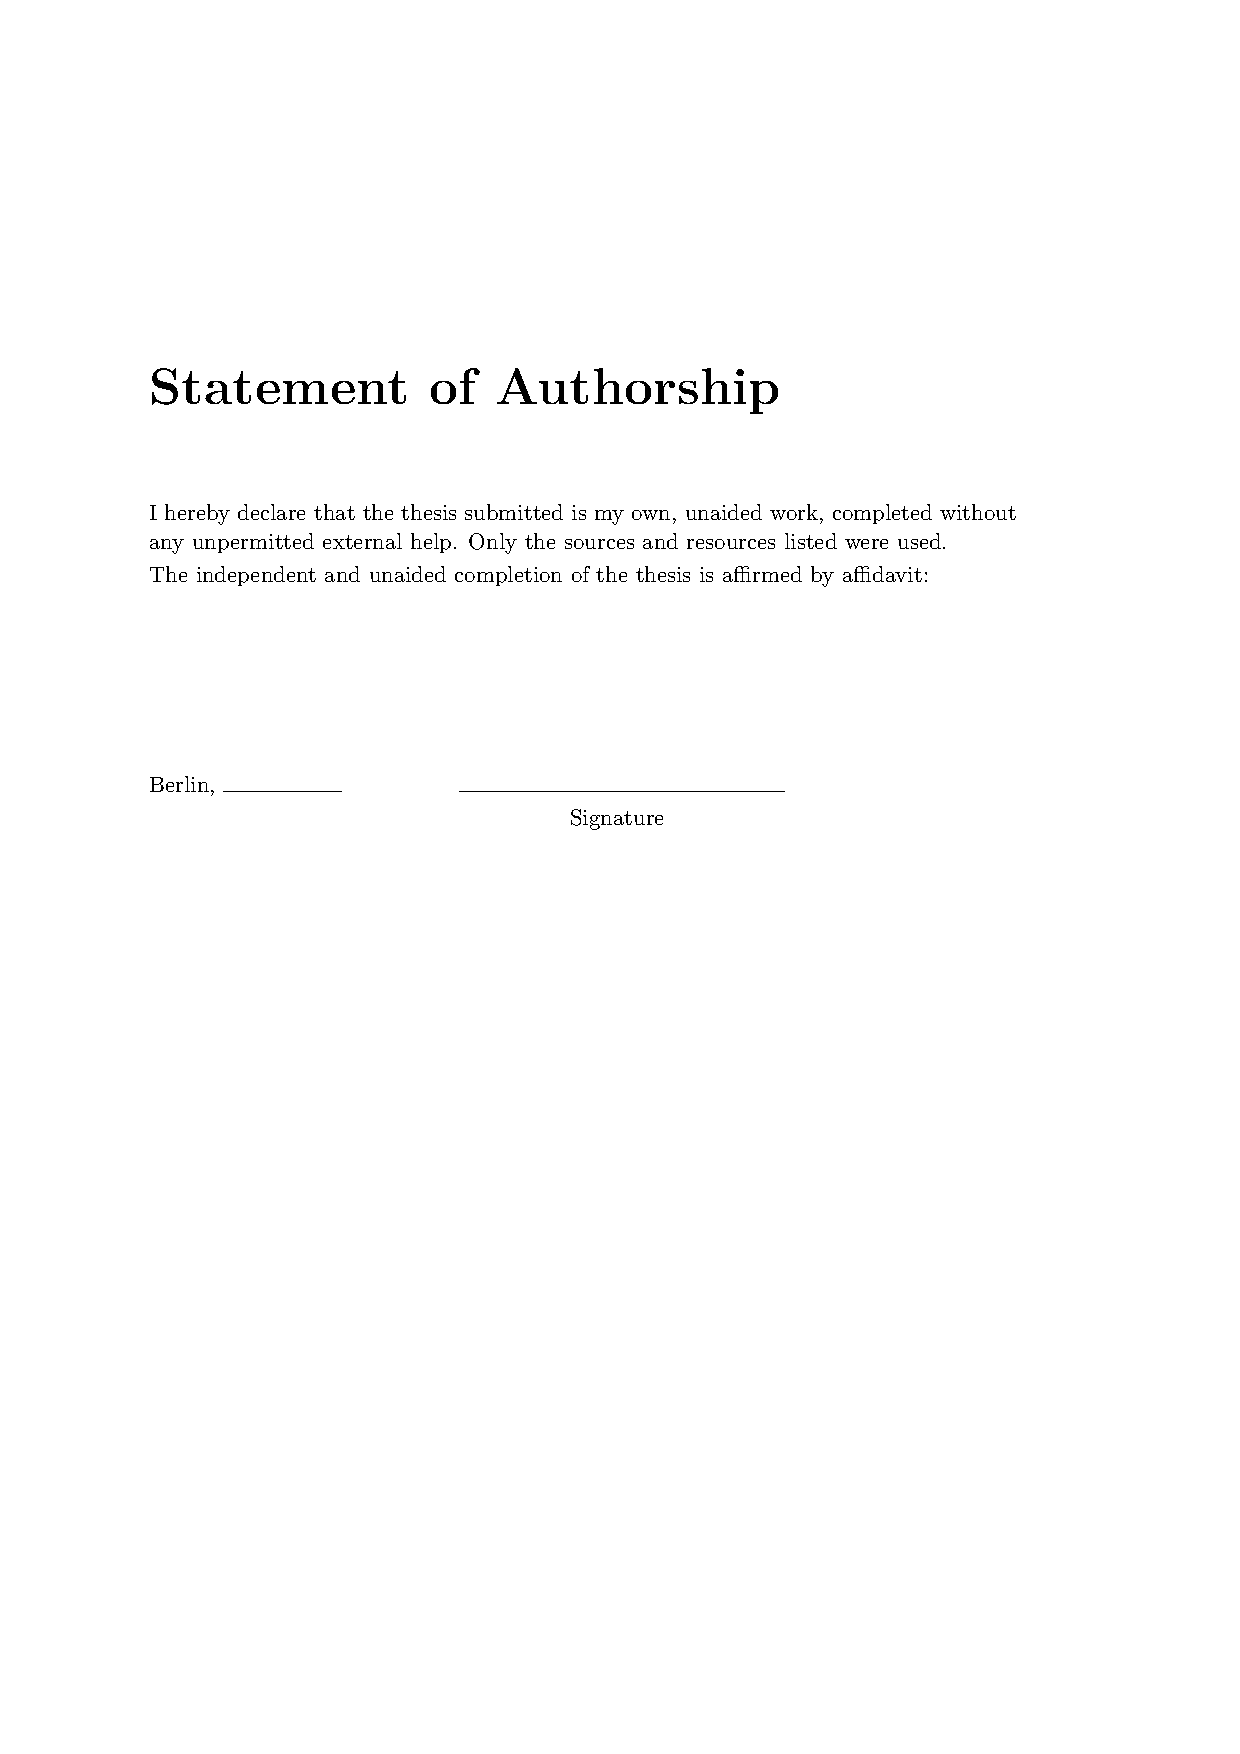
\includepdf{statement_of_authorship_exp}

\end{document}
